\documentclass[12pt]{report}

\usepackage{amsmath}
\usepackage{listings}
\usepackage{graphicx}
\usepackage{caption}
\usepackage{verbatim}
\usepackage{float}
\usepackage{pgfplots}
\usepackage{subcaption}
\usepackage{caption}
\floatstyle{plaintop}
\restylefloat{table}
\title{Self-assembly mechanisms for evolutionary robotics}
\author{Eirik Jakobsen\\ Christopher Tannum}
\date{December 2015}

\DeclareCaptionType{captioneq}[][List of equations]
\captionsetup[captioneq]{labelformat=empty}

\begin{document}

\begin{titlepage}
    \begin{center}
    
    	\vspace{1cm}
		
		\large
		\textbf{TDT4501 Computer Science, Research Project\\}    
		
		\vspace{0.5cm}		
		
		\small    	
    	\textbf{Autumn 2015}
    	
        \vspace{5.2cm}
        
        \Huge
        \textbf{Self-assembly mechanisms for evolutionary robotics}
        
        \vspace{0.3 cm}
        
        \large
        Norwegian University of Science and Technology
        
        \vspace{4.5cm}
        
        
        \Large
        \textbf{Eirik Jakobsen\\ Christopher Tannum}
        
        \vspace{1cm}
        
        \small
        \textbf{Advisors:\\}
    	\textit{Jean-Marc Montanier \\ Kazi Shah Nawaz Ripon \\ Pauline Haddow}
    \end{center}
\end{titlepage}


\chapter*{
    \begin{center}
        Abstract
    \end{center}
}

\tableofcontents

\newpage

\chapter{Introduction}
Every year the expansion and development of robots increases. 
We see robots being used in large military operations in the form of drones, as well as small robots in households that can vacuum your house while you are gone.
A lot of this technology has only recently been developed and it is expected that it will continue to grow and become a part of almost every aspect of society.

As a part of advancing robotics, a lot of the different functionality and behaviour of robots are being explored.
These mechanisms include self-replicating machines, artificial intelligence, self-assembly, inter-robot communication, etc.
In this study we will be exploring a robot's ability to self-assemble. 

Self-assembly is the autonomous organization of components into patterns or structures without human intervention \cite{whitesides_self-assembly_2002}.
We can observe self-assembling processes in nature at a molecular scale \cite{heylighen_science_2001} as well as at a planetary scale in the form of solar systems; each of which presents many different configurations.
There are several reasons to study self-assembly.
One reason is, the cells in the human body self-assemble, so understanding this mechanism can help us understand life and the prerequisites for it.
In chemistry it has been discovered that polymers can self-assemble from monomers in order to form materials that can be used in a wide range of applications\cite{chung_use_2004}\cite{siracusa_biodegradable_2008}. 
In electronics, the self-assembly of nano particles can be used to create certain semiconductors such as solar panels\cite{henini_chapter_2008}.
In either case, understanding and controlling self-assembly is essential.

Self-assembly is also used as a practical strategy for making nano structures as well as providing beneficial characteristics to the field of robotics.
In a more general sense, self-assembly can improve the movement of robots by being able to overcome larger obstacles in the environment and having a large sensory field by grouping the sensors in a self-assembled structure.

According to \cite{yim_modular_2007}, there are three main characteristics that self-reconfigurable systems benefit from.
The first is versatility, systems can self-assemble into new structures based on the specific task it is to solve.
For example, the system may change from a rolling robot to a snake robot depending on the situation.
The second characteristic is robustness.
Since the robots are usually homogeneous, one can replace broken robots to repair the system.
It is also possible to automate this process, leading to self-repair which makes the system more robust than other traditional systems.
The last characteristic is the potential low cost of developing a self-reconfigurable system.
Constructing many of the same type of robot generally lowers the overall robot cost.
In addition, there are many complex machines that can be built from  a reconfigurable system that saves cost through reuse and generality.
There are clear benefits of using self-assembly mechanisms in robotics.
However, there have been many different approaches to try to achieve self-assembly in different systems of robots.

Self-assembly can form many different configurations based on the topology of the organized structure.
In addition, self-assembly systems vary in their ability to reconfigure and disassemble depending on the challenges the environment provides.
One class of self assembly systems is stochastic reconfiguration. 
With stochastic reconfiguration the robots do not have movement capabilities themselves. 
The robots are moved passively by the environment, and bind to each other on random collisions\cite{gro_autonomous_2006}. 
With this form of reconfiguration, the reconfiguration time can only be guaranteed statistically\cite{yim_modular_2007}.
\cite{bishop_programmable_2005} demonstrates how robots named "programmable parts" can self-organize through passive movements provided by the environment. Systems that use stochastic reconfiguration are most common at micro level environments, and only achieve self-assembly because of the influence by their environment.
These characteristics do not conform to what we are trying to study, so this study will not delve further into this topic.

A crucial part of this study is to observe how self-assembly can transpire as an emergent behaviour through machine learning.
A robot that can improve its performance based on past observations is said to use some form of machine learning.
The main competing algorithms for machine learning in self-assembly robot systems, as of writing, are reinforcement leaning and evolutionary algorithms.
This study will look at machine learning and self-assembly from an evolutionary algorithms point of view.

This study covers how to implement machine learning in a system that takes advantage of self-assembly.
In particular, how self-assembly can be used in conjunction with evolutionary robotics.
Evolutionary robotics represents a way to automate the design of control systems for autonomous robots, using algorithms based on Darwinian evolution \cite{trianni_evolving_2004}.
Evolutionary robotics is a field of research that lies under the field of artificial intelligence. 
The main purpose of evolutionary robotics is to develop autonomous robot controllers that solves a given task which is not directly programmed by a human.
Evolutionary robotics takes advantage of selective reproduction based on how well the robots solve a certain task.
The controller of a robot is most often represented with an \emph{artificial neural network} where the parameters of the neural network are set by an evolutionary algorithm.

There have been previous studies about using machine learning to promote self-assembly\cite{trianni_evolving_2004}\cite{montanier_adaptive_2014}\cite{li_co-evolution_2015}. 
However, many of these studies uses differing self-assembly mechanisms such as the architecture used by the self-assembly system, the actions that are performed by the robots to achieve an organized structure and the docking mechanism hardware.
In addition, the studies have not compared the difficulty of environments in regards to the effect it can have on self-assembly.
Another element this study aims to explore is adding a local communication module to give the robots the ability to communicate simple messages within a self-assembled structure.\\ \\
\textbf{The motivation of this research is to analyse if any of these mechanisms are superior in terms of promoting self-assembly in regards to learned robot controllers and the effect it may have on the self-assembled structure's behaviour.\\ \\}
The experiment will be done in simulation with the Roborobo platform. 
Roborobo is a light-weight multi-platform simulator for extensive robotics experiments, based on basic robotic hardware setup.
The experiment is a simple predator/pray scenario, where the evolved robots(prey) can self-assemble to gain certain advantages over its pray.
While creating the simulation, great care has been taken into making most of the parameters of the system configurable.
This is done so that testing the different mechanisms is simple, such that we can compare how introducing different mechanisms effects the robot's ability to self-assemble and the behaviour of the robots.

\section{Thesis objectives}
The main focus of this study is to compare the different mechanisms that influences self-assembling robots that are governed by machine learning. 
Relevant mechanisms are the self-assembly architecture, the assembly protocol and docking(assembly) mechanisms. 
The main objectives of this study includes:

\begin{itemize}

\item Implement and explain a simulation that uses various self-assembly mechanisms such as a self-assembly architecture and an assembly protocol.

\item Compare and analyse the results of the simulation. 

\item Based on the analysis, make a conclusion as to the advantage of using certain implementations of self-assembly mechanisms and the environment in which they reside.

\end{itemize}

\section{Problem statement}
The scope of this study covers the self-assembly mechanisms in a system of robots. 
The grand question this study is trying to contribute to is:\\ \\
\textbf{How does the elements present in a system of robots influence the emergence of self-assembly when the robots are given basic learning capabilities?\\ \\}
To get a better understanding of this field, this study will present methods and analysis to answer the following questions:

\begin{itemize}

\item In what way does an evolved assembly protocol influence the robot’s ability to achieve self-assembly?

\item How does the connection port configuration, provided by the docking mechanism, influence the systems ability to self-assemble?

\item How does changing the robot environment difficulty change the systems ability to self-assemble?

\item How does introducing local communication between the robots influence the self-assembled system's behaviour?

\end{itemize}

\section{Structure of report}
The first chapter following the introduction is chapter \ref{ch:background} presenting the state of the art. It explores the field of self-assembly robotics as well as machine learning with an emphasise on evolutionary algorithms. The goal of this chapter is to present the self-assembly mechanisms which are used to categorize different self-assembly systems. In addition, machine learning is introduced with an in-depth look at off-line and on-line evolutionary algorithms. Chapter \ref{ch:methodology} contains the system description and implementation, including modifications which were made to the existing \emph{roborobo} framework. Chapter \ref{ch:results_and_discussion} describes the results from the experiment and an analysis and reasoning for their given state.
Chapter \ref{ch:conclusion} concludes the study including personal thoughts about future work.

\clearpage

\chapter{Background}
\label{ch:background}
The purpose of this chapter is to introduce the background and main concepts required to describe and compare self-reconfiguring robotic systems.
The beginning of this chapter includes a section of related work comparing similar projects and experiments.
Following, this chapter reviews the state-of-the-art of self-assembly mechanisms.
This includes the assembly architecture, protocol and different hardware mechanisms for real world application.
This chapter also reviews any additional theory that is needed for the implementation and analysis of this experiment such as machine learning and artificial neural networks.

\section{Related work}
Self-assembly in robotics is a relatively new field of research, however there are still some papers which attempts to discuss and compare the different mechanisms in a self-assembly system. 
\cite{murata_self-reconfigurable_2007} mainly covers the potential of reconfigurable systems, as well as the challenges of self-reconfigurable robotics. 
Though this article does not conduct any experiment, it does touch upon some of the same issues that this report is trying to outline.

\cite{yim_modular_2002} is an article released in 2002 that tries to explain how modular robots can self-reconfigure to solve different tasks. 
In particular, this article looks at \emph{PolyBot} and how it is able to reconfigure into different shapes. 
\cite{yim_modular_2002} also covers some of the benefits in general of having a self-reconfigurable system, as well as challenges that are still being explored.

\cite{yim_modular_2007} is the more complete and detailed of the articles presented here. 
In addition to the general benefits and challenges of modular self-reconfigurable robot system, it also looks at the different architectures the system can take, application areas and history of the field.
The article also includes an extensive list containing many self-reconfigurable modular systems and the type of architecture they have.

These papers outline what a modular self-reconfigurable system is and what the benefits and challenges of these systems are.
However, there are no direct comparison between the mechanisms themselves.
\cite{yim_modular_2007} introduces many different systems that work quite differently, but there is no conclusion based on if  these systems promote self-assembly or not.

\section{Complex systems}
\label{sec:complex_systems}
What separates complex systems from what we determine "simple systems" is that the behaviour of the system cannot be understood by simply looking at individual parts of the system.
The way the parts act together and how they are connected is what gives rise to complex behaviour.
This concept bring us to emergent behaviour.
Emergent behaviour is a process where the system takes on certain patterns, regularities or form larger entities through the interconnections and interactions among simple parts that by themselves to not portray such properties.
Further, this report will look at an emergent behaviour known as self-assembly.  

In nature one can find many examples of complex systems displaying self-organizing behaviour.
The collectives range from just a few individuals to millions.
Some examples are flocking behaviour in birds, fish schooling, and the complex societies seen among social insects(Figure \ref{fig:collective-behaviour}). 

\begin{figure}[H]
	\centering
	\begin{subfigure}[b]{0.31\textwidth}
		\label{fig:flocking}
		\centering
		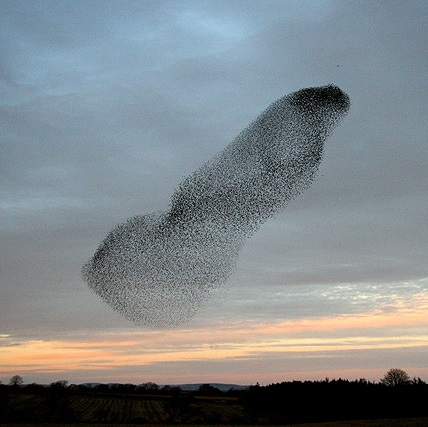
\includegraphics[height=\linewidth]{chapters/res/flocking_edit.jpg}
		\caption{Flocking\cite{baxter_flocking.jpg_2008}}
	\end{subfigure}
	\begin{subfigure}[b]{0.31\textwidth}
		\label{fig:scholing}
		\centering
		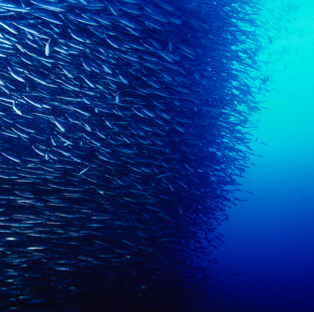
\includegraphics[height=\linewidth]{chapters/res/schooling_edit.png}
		\caption{Schooling\cite{polyglottus_mockingbird-tales-readings--animal-behavior-5.1.pdf_2011}}
	\end{subfigure}
	\begin{subfigure}[b]{0.31\textwidth}
		\label{fig:social-insects}
		\centering
		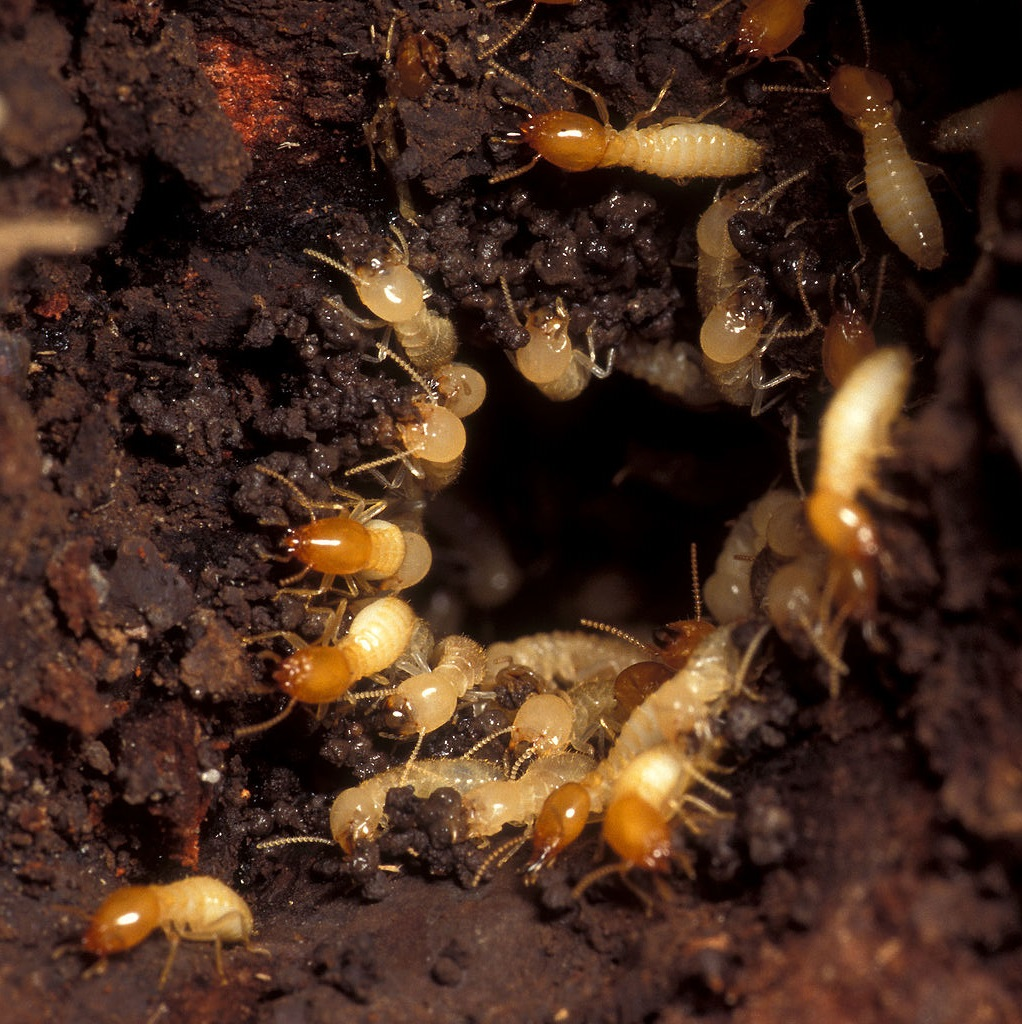
\includegraphics[height=\linewidth]{chapters/res/Termites_rush_to_damaged_portion_of_mound_edit.jpg}
		\caption{Termites\cite{bauer_termites_rush_to_damaged_portion_of_mound.jpg_2007}}
	\end{subfigure}
	\caption{Examples of self-organizing behaviour in nature.}
	\label{fig:collective-behaviour}
\end{figure}

Social insects such as termites build large structures featuring complex architectures.
These examples show how a collective of simple agents, without a central controller can accomplish tasks each individual would be unable to perform themselves. 
Together, the actions of these agents form a collective behaviour that can be considered intelligent.  

These biological systems display massively parallel, decentralized computation.
This stands in contrast to conventional computer systems with a central processing unit executing instructions serially.
Research into self-assembling robot systems therefore take inspiration from biology, using methods such as evolutionary algorithms simulating Darwinian evolution, and artificial neural networks inspired by the way brains process data.




\section{Self-assembly architectures}
\label{sec:sfArchitecture}
Self reconfiguring robots can assemble into many different shapes, and there are many ways to do so.
We define these properties as the self-assembly architecture.
Each architecture presents different challenges and benefits.
The architectures can in broad terms be categorized either as non-mobile- or mobile-architectures.
The non-mobile architectures are characterized by the topologies of the structures they form, while mobile architectures are characterized by having more mobile robots with a higher degree of freedom.
This section will describe and define some of the common assembly architectures used in previous projects.
\subsection{Non-mobile Architecture}
Typically these robots have little mobility themselves, but can form complex structures capable of a wide range of behavior.
One of the long term visions for these kinds of robots is called "bucket of stuff"\cite{yim_modular_2007}.
The idea is to have a collection of different robot modules which can be assembled on demand to solve different tasks.
One way to classify non-mobile robots is based on their configuration topology.
The main classes for configuration topologies are chain and lattice configurations.

\subsubsection{Chain topology}
The chain topology is a configuration where each robot is connected in a serial architecture.
The robots can form many different shapes to represent creatures such as snakes, spiders or other configurations needed to complete its task.
One of the challenges with this topology is coordinating movement and decisions as information has to be propagated serially.
Examples of chain architecture based robots are Molecubes\cite{zykov_molecubes:_2007}, Yamor\cite{mockel_yamor_2006}, and Conro\cite{castano_conro:_2000}.
Yamor is depicted in figure \ref{fig:yamor}.

\begin{figure}[H]	
	\centering
	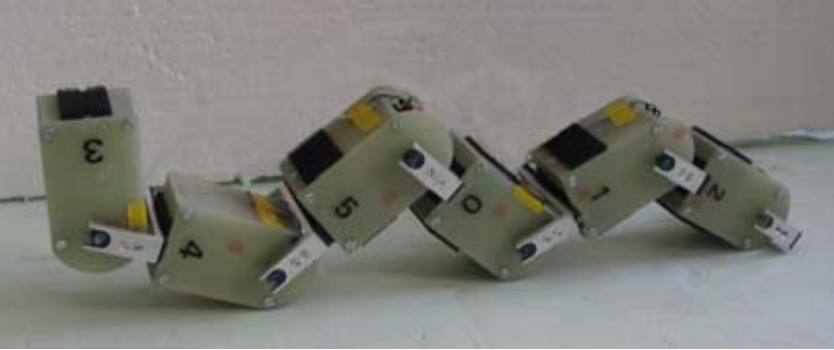
\includegraphics[scale=0.5]{chapters/res/Yamor.PNG}
	\caption{Yamor robots configured as a snake\cite{mockel_yamor_2006}.}
	\label{fig:yamor}
\end{figure}

\subsubsection{Lattice topology}
The Lattice architecture is a configuration where robots are arranged in a grid/lattice topology.
The robots can then execute motion and control in parallel which provides a simpler configuration in comparison to the chain architecture. 
Examples of lattice architecture would be a cubic or hexagonal grid.
Due to its simplicity, a lattice architecture is easier to scale. 
There have been more research groups working on this class of architecture due to its easier implementation \cite{yim_modular_2002}.

Symmetry is a desirable property for robots that employ the lattice architecture because this makes reconfiguration into new positions in the grid easier.
To maintain the symmetry property in 3D space, each robot needs more connection points and actuators than in 2D space\cite{murata_self-reconfigurable_2007}.
This complicates the design of the robots. 
Thus, building these robots with a high enough power/weight ratio is difficult.
Examples of lattice architecture based robots which is able to perform self-reconfiguration are ATRON\cite{brandt_atron_2007}, Miche\cite{gilpin_miche:_2008}, and Catoms\cite{kirby_catoms:_2005}.
Atron is depicted in figure \ref{fig:atron}.

\begin{figure}[H]
	\centering
	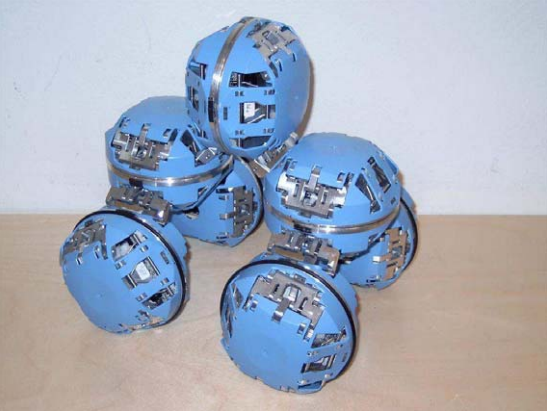
\includegraphics[scale=0.5]{chapters/res/Atron.png}
	\caption{Atron assembled into a four wheeled car \cite{brandt_atron_2007}.}
	\label{fig:atron}
\end{figure}

\subsection{Mobile architecture}
Mobile architectures are characterized by having autonomous robots which can self-assemble and reconfigure themselves.
Each robot can operate independently or form larger structures when needed, by hooking up with other units.
The structures formed may have different topologies and can coordinate their movements to form a larger virtual network\cite{yim_modular_2007}.
One example of a mobile architecture is presented in \cite{gross_object_2006}.
In the experiment depicted in figure \ref{fig:swarmbot-object-transport}, a group of robots are programmed  to move an object which requires cooperation by being to heavy for a single robot to move.

\begin{figure}[H]
	\centering
	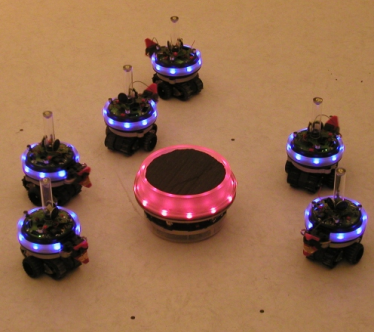
\includegraphics{chapters/res/MobileObjectTransport.png}
	\caption{A group of swarmbots(blue) preparing to transport an object(red)\cite{gro_autonomous_2006}.}
	\label{fig:swarmbot-object-transport}
\end{figure}
Since each robot in the architecture is autonomous one challenge is making the individual robots cooperate.
This is especially difficult in cases where the optimal solution to a task involves cooperation, but the robots are able to complete the task individually.
This challenge is demonstrated in \cite{trianni_evolving_2004} where the researchers were able to promote self-assembly to solve the task, but the self-assembly was only present in 2 out of 10 trials.

The high degree of mobility in each robot allows them to form a wide variety of topologies to solve tasks, but this also makes reconfiguration more difficult for large robot swarms.
Because of this difficulty there has been less research into mobile architectures.

Experiments conducted demonstrates robots solving simple tasks such as object transport\cite{gro_autonomous_2006}, phototaxis\cite{trianni_evolving_2004}, and energy collection\cite{montanier_adaptive_2014, weel_emergence_2012}.
These experiments demonstrate that mobile robots are capable of solving tasks through self-assembly.
But the tasks presented are trivial problems and do not reflect the complexity of real world problems.
Before solving real world problems, future research need to demonstrate a greater amount of robots cooperating.
Additionally, robots that have the ability to take different roles when solving problems as well as cooperating when solving multiple problems presented by the environment.

\section{Hardware mechanisms}
\label{sec:hardware}
Several robot systems that are capable of self-assembly have been developed over the years\cite{gross_self-assembly_2008, wei_sambot:_2011, brandt_atron_2007}.
Even though some vary greatly in implementation, all these robots have some sort of hardware which makes it possible to perform self-assembly.
The hardware available in each robot is influenced by the desired assembly architecture.
However, some common properties can be identified.  

\section*{Prerequisites for self-assembly}
The robots must have some form of \emph{movement} to reach each other.
This movement can be provided by the hardware available or from external sources.
Similar to movement, the robots require a \emph{docking mechanism} to physically connect to other robots in order to self-assemble.

The requirements described can be considered as minimum requirements for self-assembly, but for more advanced behaviour, the robots need additional hardware utilities.
If the robots are to be self-assembled without human intervention, they need a \emph{discovery mechanism} to detect the presence of each other.
To coordinate behaviour, the robots also need a \emph{communication mechanism} capable of receiving and sending information.
These requirements are very general and can be achieved in a wide variety of ways. Table \ref{tab:hardware-mechanisms} describes some methods to complete the discovery and communication requirements.

\begin{table}[H]
	\centering
	\caption{Various hardware solutions to discovery and communication.}
	\begin{tabular}{ | l | l | l |p{5cm} |}
		\hline
		& Chain 						& Lattice \\ \hline
		Discovery 		& IR\cite{castano_conro:_2000}  & IR\cite{gilpin_miche:_2008} \\ \hline
		Communication 	& 1-wire bus\cite{zykov_molecubes:_2007}, IR\cite{castano_conro:_2000}, Bluetooth{\cite{mockel_yamor_2006}} & IR\cite{brandt_atron_2007, gilpin_miche:_2008}  \\\hline
	\end{tabular}
	
	\label{tab:hardware-mechanisms}
\end{table}


It is possible to simplify or ignore some of these requirements, but self-assembly is impossible without the docking mechanism.
This means that the choice of docking mechanism can be a deciding factor in the performance of a self-assembling robot. 


\subsection{Docking mechanisms}
\label{sec:mechanisms}
The docking mechanism is an essential component in self-assembly, and has been solved in various ways in previous studies.
For experiments with self-assembly in simulation, the mechanisms are often simplified since the focus of the experiments usually is the self-assembly behaviour.
Therefore, it can be difficult to replicate the results on real hardware.
The real world introduces noise, and the mechanisms designed must be able to cope with that imperfection.
This is especially true in the context of machine learning as the resulting controllers are rarely optimal.
The desired self-assembly architecture also plays a role in designing a docking mechanism.

\subsubsection*{Male-female connector}
This form of connection mechanism is used by the ATRON\cite{brandt_atron_2007} robots.
The male modules are shaped like three hooks that can lock onto female connector bars.
Each robot has eight connector modules, and are arranged such that every second connector is male and every second is female.
This allows each robot to connect to a maximum of eight other robots.
A disadvantage with this type of mechanism is that the robots have to match the male to the female connectors before they can assemble, which eventually complicates the docking procedure.
\subsubsection*{Gripper and ring}
The swarm-bot platform\cite{gro_autonomous_2006} uses this mechanism for self-assembly in the real world.
Each robot is equipped with a gripper, and is surrounded by a ring matching the gripper. 
This means that each robot can initiate one connection to other robots, but multiple robots can connect to each ring.
There are several advantages with this mechanism; it allows some misalignment that makes docking simpler and the ring makes it possible for several other robots to connect.
Although many robots can connect to the ring, having only one gripper limits the possible configurations.
This disadvantage can be mitigated by adding more grippers.

\subsubsection*{Magnetic docking mechanisms}
These mechanisms typically use one or more magnets to form connections.
One desirable property these mechanisms have, is that they can tolerate some noise/misalignment since the magnet connectors can compensate by attracting each other.
One problem with using magnets is that robots wishing to connect have to make sure that they have the magnets in the right polarity to attract each other.
Also, if electromagnets are used, they have to power them continuously to maintain the connection which increases power consumption.

\paragraph*{Magnetic slip-ring}
This mechanism is used in simulation by \cite{weel_emergence_2012}.
The magnetic slip ring can be set to either a positive, negative, or neutral state.
A connection will be made if at least on of the robots have their slip-ring set to positive, and neither of them have it set to negative.
For simulation purposes, it is assumed that the connection immediately becomes rigid.

\paragraph*{Surfaces with magnets}
The Molecubes\cite{studer_spontaneous_2006} also use magnets to form connections.
The Molecubes has flat connection surfaces with electromagnets which can be turned on, or off to create connections.
Each cube has four connector surfaces, which means that each cube can connect to four other cubes.

\paragraph*{Permanent magnets and springs }
\cite{murata_hardware_2000} describes this mechanism.
Unlike the two magnetic mechanisms previously described, this mechanism uses rare earth permanent magnets.
The magnets are separated by two springs and a shape memory alloy(SMA) coil.
The springs are designed to have a slightly lower force than the magnets when they are compressed.
The mechanism detaches by applying an electrical current to the SMA, extending it to the memorized length.


\section{Assembly protocols}
\label{sec:protocol}
In the context of swarm robotics and this paper, the term assembly protocol is defined as the sequence of actions that has to be performed before a successful self-assembly can occur. 
For pre-programmed robots the protocols is determined by the programmer, and known in advance.
Evolutionary robotics are different in this regard since the controllers are evolved, therefore, the resulting assembly protocols may be unexpected. 
An overview of assembly protocols used in previous projects is presented in table \ref{tab:protocols}.
As for a specific model of an assembly protocol, we have two main approaches. 

\begin{table}[H]
	\centering
	\begin{tabular}{ | l | c | c | c | p{5cm} |}
		\hline
		& Pre-determined & Evolved & Reference\\ \hline
		CONRO & X & & \cite{castano_conro:_2000}\\ \hline
		Miche & X & & \cite{gilpin_miche:_2008}\\ \hline
		SWARM-BOTS project & X & X & \cite{gross_object_2006, trianni_evolving_2004}\\ \hline
		N/A & & X & \cite{weel_emergence_2012}\\ \hline
	\end{tabular}
	\caption{An overview comparing past research projects of swarm robots based on the robot controller being evolved using an evolutionary algorithm, or pre-programmed for its intended usage.}
	
	\label{tab:protocols}
\end{table}

\subsection{Pre-determined assembly protocol}
The traditional approach is to use an assembly protocol which is determined by the programmer in advance.
This means that the assembly protocol is embedded in the controller software and does not change without reprogramming. 

An example of a pre-determined protocol is found in \cite{gross_object_2006}.
In this experiment, the s-bots uses RGB LEDs to signal their position, and if other s-bots should dock with them.
The lights are also used to determine if the self-assembly process is complete. 

Using the protocol described, the s-bots are successfully self-assembled in 26 out of 30 trials. The advantage of using a pre-programmed assembly protocol is that it can be tailored to the problem. This often leads to good performance and a predictable outcome of the assembly once the system is deployed. It does however carry the disadvantage of being less general in the sense that the protocol can only be changed by implementing new software. Depending on the assembly protocol, it can also be quite complex which in turn, makes the implementation more difficult.

\subsection{Learned assembly protocol}
In a machine learning setting, we can give the robots docking mechanisms, but leave the entire assembly protocol up to the learned controller.
One might ask why machine learning, where the resulting controller rarely is optimal, is a good approach when pre-determined protocols can be developed instead.
According to \cite{russell_artificial_1995}, there are three main reasons for why we would want a robot to learn.
First, the programmer may not always have the ability to foresee all the situations the robot may encounter.
The robot must then learn from its observations if it is to solve the probable new set of problems.
Second, the programmer cannot predict all changes that happen over time. 
If we had some system that tried to anticipate tomorrow's weather, then it must be capable of analysing based on new sets of observation which were unknown at the time of system's design.
And finally, the programmer may not even know the solution to the problem themselves, such that the system itself must find the solution.
This last reason is especially interesting in accordance with self-assembly as we do not always know when it is appropriate to employ self-assembly for solving a certain problem.

An example of a type of learned assembly protocol is found in \cite{trianni_evolving_2004}. 
This example uses s-bots each of which uses an \emph{artificial neural network} to control them. 
The neural network controls all of the input and output signals of the s-bot.
This also includes the use of the gripper(docking mechanism) and the loudspeaker(produces sounds that can be used for communication between the robots).
Using a simple genetic algorithm, they were able to evolve an assembly protocol in 2 out of 10 trials.

Even though an assembly protocol was evolved, the desired results of using the loudspeaker to signal position and performing self-assembly were inconclusive.
The s-bots rather used exploits such as lining up against the wall of the experiment to perform a simpler self-assembly.
The results also showed that the loudspeaker was not used optimally and was something they would like to explore in future research.
This behaviour is one of the disadvantages of using machine learning to develop assembly protocols.
First of all, it may not be able to create a protocol at all, and it is also likely that the end results are sub optimal. 
A reason behind this is that the environment in which the robots are evolved often impacts the type of assembly protocol that emerges.

\section{Machine learning algorithms}
\label{sec:learning}
We say that a robot is learning if it can improve its performance on tasks in the future based on past observations.
Learning ranges from trivial matters such as writing a word to complex theories of the universe.

The learning algorithms commonly used for automatic design of controllers can be divided into two main sub domains: reinforcement learning(RL) and evolutionary algorithms\cite{brambilla_swarm_2013}.

Reinforcement learning is a class of learning algorithms where the agent learns through trial and error, receiving positive and negative feedback for its actions\cite{brambilla_swarm_2013}.
The agent records the feedback received for performing a particular action in each state.
Through this process the agent discovers which action is optimal for a given state.
Applying this form of learning to swarm robotics presents several challenges.
One challenge is the fact that a swarm performs actions as a collective, but the learning is done on an individual level and does not reward global behaviour\cite{brambilla_swarm_2013}.
Additionally traditional RL requires that the environment can be quantized into a finite number of discrete states\cite{schmidhuber_evolutionary_2000, brambilla_swarm_2013}.
The number of possible interactions between the robots and the environment, and the noise in the real world leads to a high amount of states and makes it difficult to know how these are connected in advance\cite{schmidhuber_evolutionary_2000}.
Techniques such as using an approximator\cite{brambilla_swarm_2013} to reduce the state space, and more intelligent reward mechanisms\cite{brambilla_swarm_2013}, can be used to reduce the impact of these challenges.
Several projects\cite{li_learning_2004, balch_behavioral_1998, mataric_interaction_1994} have successfully applied reinforcement learning in multi-agent systems.
Given the challenges of RL, as the goals and ambition of projects increase, researchers are drawn towards techniques that resemble evolutionary algorithms\cite{schmidhuber_evolutionary_2000}.

Evolutionary algorithms attempts to find solutions to a problem by simulating the mechanisms of Darwinian evolution\cite{trianni_evolving_2004}.
In these algorithms, the possible solutions are encoded into genomes and improved iteratively over multiple generations, where well performing individuals reproduce more and spread their genome.



\subsection{Evolutionary algorithms}
\label{sec:evo_alg}
Evolutionary algorithms is a class of algorithm in the category of \emph{bio-inspired algorithms}\cite{binitha_survey_2012}.
Nature has shown that it is a great optimizer.
When we examine features and phenomenons in nature, it tends to find the optimal strategy.
The strategies employed are often very simple, but has great results.
Bio-inspired algorithms takes inspiration from nature and attempts to mimic the behaviour observed in nature.
These algorithms can be categorized by the natural phenomenons they mimic.
The three main categories are \emph{evolution}, \emph{swarm-based}, and \emph{ecology}\cite{binitha_survey_2012}. 
These algorithms are optimization algorithms and can therefore be used to automate the design of robot controllers.
Specifically in the field of evolutionary robotics, the focus has been to employ evolutionary algorithms in the design of robot controllers.


There are many variants of evolutionary algorithms, the most common can be categorized by when the evolution takes place\cite{eiben_embodied_2010}.
\begin{quote} 
	In \emph{off-line} evolution, the evolutionary development of robot controllers takes place before the robots start their “real” operation period.
	\emph{On-line} evolution is the opposite, in that the evolutionary development of robot controllers takes place during the “real” operation period of the robots(although off-line evolution might precede on-line evolution as an educated initialization procedure)and is an ever-continuing process.\cite{eiben_embodied_2010}
\end{quote} 


\subsubsection*{Off-line}
The details of how off-line evolutionary algorithms are implemented usually vary, however most implementations perform a variation of the same following steps\cite{doncieux_evolutionary_2011}, displayed in figure \ref{fig:offline-ea}. 

The first step of an off-line algorithm is to generate some population.
There are two main procedures that can be used to generate the initial population.	 
One can either generate the genomes for the robots completely random, or by some function that applies bias.
In the biological sense, a genome contains the configuration, or blueprint for an individual.
Before the genome can be used by the robots, this configuration must be translated into a robot controller.
The translation procedure can for example consist of translating the genome into an \emph{artificial neural network}, and uploading it to the robots.
The next step after initialization is the robots acting in the environment.
After a given set of time steps, the genome is evaluated by a fitness function which scores the robots based on their ability to solve the task.	 
At the end of a generation, some of the genomes will be selected for reproduction based on their fitness.	 
The algorithm then proceeds to mate genomes through crossover and applying mutation on the population.	 
The process is repeated on this new set of genomes until the desired fitness is reached, or some processing time threshold is met.
\cite{trianni_evolving_2004, li_co-evolution_2015} describes examples of how this process can be applied to create controllers for self-assembling robots. 

\begin{figure}[H]
	
	\centering
	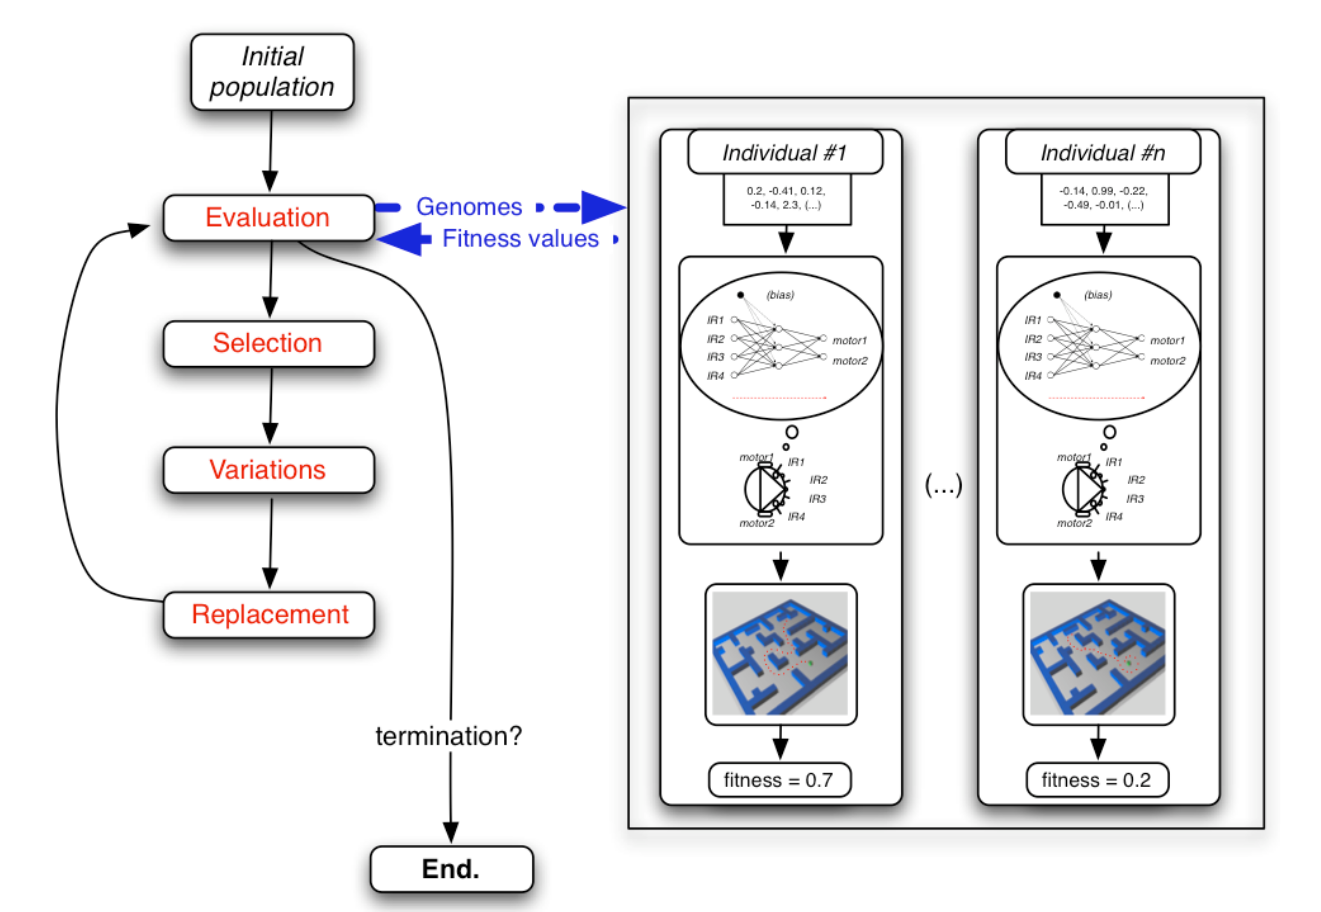
\includegraphics[width=\textwidth]{chapters/res/offline-ea.png}
	\caption{Operation of a typical EA\cite{doncieux_evolutionary_2011}}
	\label{fig:offline-ea}
\end{figure}

The evolution process requires a lot of trials to evaluate the performance of each genome. Performing these trials on real hardware is therefore impractical, time consuming, and possibly dangerous as the robots may damage themselves or the environment.
The evaluation is therefore often performed in simulation\cite{koos_crossing_2010}.
Transferring the controllers evolved in simulation to real hardware has proven to be problematic because the controllers tend to be less efficient once transferred.
This \emph{reality gap} remains a critical issue in evolutionary robotics\cite{koos_crossing_2010}.



\subsubsection*{On-line}
On-line evolutionary algorithms, in contrast to the off-line variants, does not share a well defined series of steps. Several algorithms for this category has been proposed. Among them are mEDEA\cite{montanier_adaptive_2014}, MONEE\cite{noskov_monee:_2013}, and ASiCo\cite{hutchison_task-driven_2011}. 

In mEDEA(minimal Environment driven Distributed Evolutionary Adaptation) each robot contains an active genome and a reservoir of received genomes.
The robots broadcasts their genome in a limited range to other robots.
At a pre-defined number of time steps, the robot forgets its active genome and selects a new one at random from the reservoir.
The robot becomes inactive if it runs out of genomes.
An inactive robot remains stationary for the following generation and receives genomes broadcasted from other robots.
The result is that over time, ineffective genomes are removed from the population while the more successful genomes are able to spread.

MONEE(Multi-Objective and Open-Ended Evolution) can be considered an adaptation of mEDEA.
In MONEE the robot has a life cycle consisting of two phases with a fixed duration.
The first phase is the \emph{life phase}.
In the \emph{life phase}, the robot performs tasks such moving or foraging.
When the lifetime of the robot is reached, it enters a rebirth phase and becomes an "egg".
The egg is stationary and receives genomes from other robots that are currently in their \emph{life phase}.
For the egg to select one genome out of the ones received from the other robots, MONEE introduces the concept of \emph{parental investment}.
During the \emph{life phase} the robots receive credits for performing tasks in the environment.
When a robot passes its genome to an egg, it passes the number of credits earned.
The egg then uses the number of credits to compare and select a new genome for rebirth.
If there are multiple tasks defined, the egg uses an exchange rate between the tasks based on their difficulty to compare them. 
This ensures that genomes who specialize in difficult tasks can compete with genomes that perform easier tasks. 
This system allows genomes to specialize in different tasks and therefore makes MONEE well suited for multi-objective tasks.

ASiCo(Asynchronous Situated Co-evolution) is a co-evolutionary bio-inspired algorithm that in contrast to MONEE and mEDEA uses a fitness function to decide if a robot should reproduce.
Like other on-line algorithms, multiple genomes are present among the robots even though this algorithm carries the characteristic of a fitness function from off-line algorithms.
The ASiCo algorithm works by having the robots act out some scenario and uses energy gain or loss as a performance gauge. 
Differing from off-line algorithms, ASiCo continuously evaluates the different robots' fitness asynchronously.
If a death condition is met, then the robots is either removed from the system or substituted. 
If however a situated mating condition is met, then the candidate is evaluated by its fitness.
If the candidate is acceptable, then it is allowed to reproduce.
In the case where the fitness is not acceptable, it simply continues to live on in the system.

\section{Artificial neural networks}
Computers excel at performing tasks that can be described as a series well-defined steps, and can at these tasks easily outperform humans in doing so.
Tasks that humans find easy, such as understating speech or recognizing faces has proven to be difficult to describe a series of unambiguous operations in the conventional computation model.
Biological neural networks, such as brains, have evolved to be very good at pattern recognition and data classification.
Artificial neural networks(ANN) take inspiration from how biological neural networks process data.

ANN's consist of interconnected processing units(neurons) which work in parallel to solve a specific problem.
The neurons employ a simplified model of how a biological neuron works.
The operation of an artificial neuron consists of two main components, depicted in figure \ref{fig:artificial-neuron}.

\begin{figure}[H]
	
	\centering
	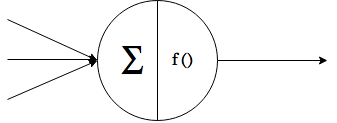
\includegraphics[width=0.5\textwidth]{chapters/res/Neuron.png}
	\caption{Model of an artificial neuron.}
	\label{fig:artificial-neuron}
\end{figure}
First, the neuron sums the action potential from the preceding neurons.
The activation function is then applied on the sum which produces a new action potential as the output.
The role of the activation function is to transform the action potential in the node to an output that can be passed to the succeeding nodes.
These functions often have a thresholding effect where the neuron outputs a low potential until a threshold is reached.
A common activation function is the logistics equation(\ref{eq:logistics-equation}).

\begin{captioneq}[H]
	\begin{equation}
	o_i= \frac{1}{(1+e^{-v})}
	\label{eq:logistics-equation}
	\end{equation}
	
	\caption{The ouput of node i with internal action potential v.}
\end{captioneq}

The connection strength between neurons is simulated by introducing weights on the connections.
A neuron with a higher weight on one of its connections will then be more influenced by that particular connection.
Learning can then be performed by modifying the weights on the connections in the ANN.


The neurons in ANN's are organized into multiple layers, where each neuron is connected to the neurons in the preceding layers.
Typically there is a input layer, an output layer, and zero or more hidden layers between them.

\begin{figure}[H]
	\centering
	\includegraphics[width=0.8\textwidth]{chapters/res/Simple-MLP.png}
	\caption{A feed forward network.}
	\label{fig:mlp-simple}
\end{figure}

Figure \ref{fig:mlp-simple} depicts a simple feed forward network with one hidden layer.
The inputs are propagated from the input layer on the left to the output layer.
More complex network topologies introduce connections within the layers and connections back to preceding layers.

Creating good robot controllers can be difficult as the number of sensors and actuators grow.
The designers may know what desired behavior for the robots is, but expressing this in the conventional computing model as a series of instructions can be difficult.
Instead, with machine learning an ANN can learn from examples of desired behavior provided by the controller designers.
This approach allows designers to create the desired controllers by providing examples instead of knowing the exact solution.

Neural networks have been applied to design robot controllers in several\cite{trianni_evolving_2004, montanier_adaptive_2014, brandt_atron_2007} self-assembling robot systems.
These robot systems all use different approaches in how neural networks are applied to create the controller.
\cite{montanier_adaptive_2014} uses a simple feed forward network, while \cite{trianni_evolving_2004} uses a CTRNN, and finally \cite{brandt_atron_2007} uses multiple neural networks which decide different parts of the behavior.
This shows that neural networks are a versatile tool in designing robot controllers for self-assembling robot systems.


\clearpage

\chapter{Methodology}
\label{ch:methodology}


\section{Experiment motivation}
The introduction lists several questions that this report should contribute to.
One of the questions concerns how collective decision making influences the emergence of self-assembly.
Swarm behaviour found in nature displays how simple agents collectively can make a decision.
The goal of this experiment is therefore to design a similar environment to promote this form of collective behaviour.
In this environment the robots have to form swarms for survival, and collectively decide if they should self-assemble or attempt an escape.

The experiment also allows investigation into the other questions this report contributes to.
By varying the parameters of the experiment it is possible to observe how different docking mechanisms and assembly protocols influence the self-assembly behaviour of the robots.
Section \ref{sec:results} further describes how this experiment can answer these questions.
\section{Experiment setup}
\label{sec:description}
For this experiment a micro-organism environment is imagined, where the organisms find themselves in some liquid pool. 
The micro-organisms are the agents in our system and are represented as swarm bots.
The main functions of the robots are, in addition to movement, foraging and self-assembly.

The robots find themselves in a pond.
In the pond there are nutrients which the robots can feed on to replenish their energy.
At the same time the pond also contains larger predator organisms which wants to feed on the robots.
It is imagined that the robots can assemble to form larger structures.
The robots can protect themselves from the predator organisms by forming a larger structure which the predator is unable to eat.
When the robots are assembled they may eat the larger predator to replenish energy as well.
The predators come in multiple sizes, and to gain an advantage the robots must form a large enough structure.
Maintaining the assembled structure cost energy, and the robots therefore have an incentive to disassemble once the structure is no longer required.

\section{Environment}
The imagined pond environment can be represented as a rectangular box(figure \ref{fig:environment}), containing the robots, nutrients and predators.
Initially the environment is populated with nutrients, robots, and predators placed at random positions in the environment.
When a nutrient is consumed, a new one is placed at a random position in the environment.
Additionally, to ensure fairness the predators cannot be placed within a threshold radius of a robot. 

\begin{figure}[H]
	
	\centering
	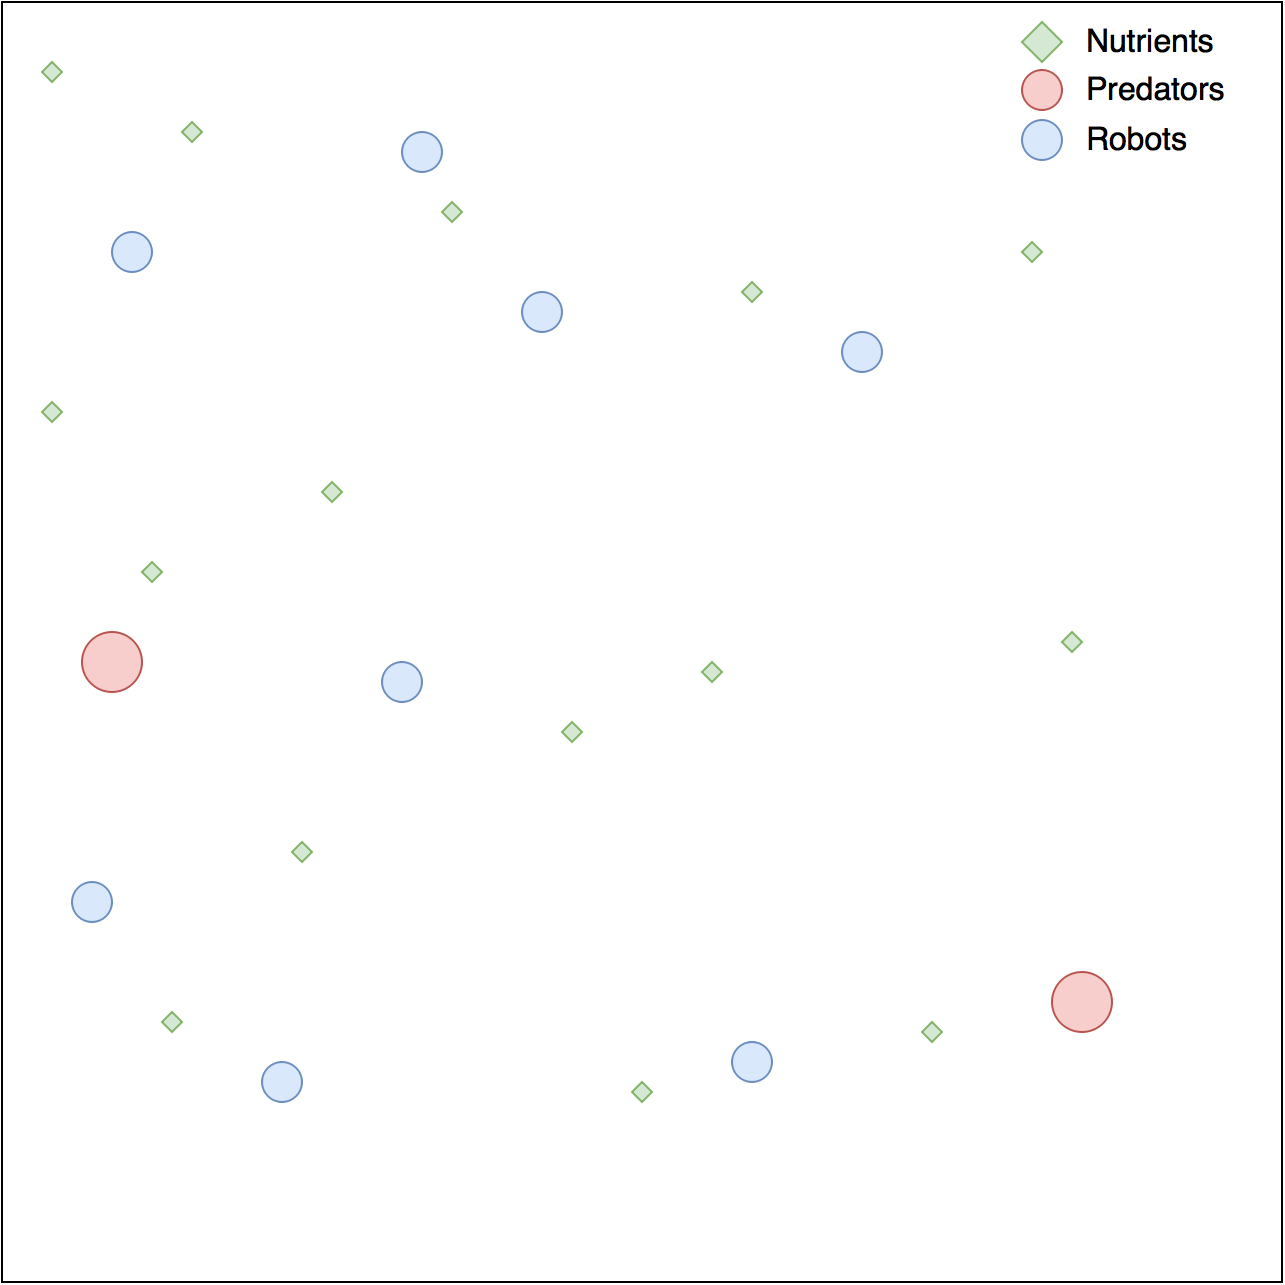
\includegraphics[width=0.65\textwidth]{chapters/res/Environment.png}
	\caption{Initial configuration of the environment.}
	\label{fig:environment}
\end{figure}

\section{Roborobo overview}
The programming interface for roborobo is divided into three main components(\emph{World observer, Agent observers, Agent controllers}).
Each robot in the simulation receives an instance of the \emph{agent controller}, and an instance of the \emph{agent observer}.
The philosophy of the roborobo framework is that the programmer should implement the robot behavior in the \emph{agent controller}, and use the \emph{agent observer} and \emph{world observer} to access state about agents and the world.
This relationship is visualised in figure \ref{fig:component-relationship}.

\begin{figure}[H]
	\centering
	\begin{subfigure}{0.31\textwidth}
		\label{fig:controller}
		\centering
		\hspace*{1.15cm}\includegraphics[height=\linewidth]{chapters/res/agent_controller.png}
		\caption{}
	\end{subfigure}
	\begin{subfigure}{0.31\textwidth}
		\label{fig:agent-observer}
		\centering
		\includegraphics[height=\linewidth]{chapters/res/agent_observer.png}
		\caption{}
	\end{subfigure}
	\begin{subfigure}{0.31\textwidth}
		\label{fig:world-observer}
		\centering
		\includegraphics[height=\linewidth]{chapters/res/world_observer.png}
		\caption{}
	\end{subfigure}
	\caption{The relationship between a)the agent controller, b)the agent observer, and c)the world observer. }
	\label{fig:component-relationship}
\end{figure}

Each robot in the simulation also receives a component called a \emph{world model}.
The world model contains the representation of the outside world that the agent is aware of.
This includes state such as sensors readings and current velocity.

The observers can be used to perform tasks that are not directly related to the robot behavior.
In each simulation step the observers are run before any of the \emph{agent controllers} are run.
This means that the observers have a stable snapshot of the world between each update.
The observers are therefore useful for performing tasks that should be performed between each update of the world.
Examples of useful applications of the observers is updating the agent world models, monitoring, logging, computing fitness, and managing evolutionary algorithms.
In the standard case, understanding the components described in this section is sufficient to perform a wide variety of simulations.


The experiment described in this chapter does not fit within these bounds, the necessary modifications to the framework is further described in section \ref{sec:modifications}.



\section{Roborobo modifications}
\label{sec:modifications}
	\subsection{Robot Groups}
	As mentioned in the description, roborobo does not support self-assembly out of the box.
	Self-assembly support therefore requires adding additional abstractions to roborobo.
	The high level abstraction that encapsulates the behavior for connected robots is called a \emph{Robot group}.
	All robots that are capable of self-assembly are robot groups.
	This means that single robots that are not connected are simply robot groups with one member.
	The responsibilities of the robot group is to take care of group movement, handling collisions, connecting and disconnecting. 
	\subsubsection{Movement}
	In the roborobo framework the robots movement is decided by the robot controller by requesting a certain angular and translational velocity.
	The movement of a group is decided by first converting the desired direction and velocity into a translation vector.
	\begin{equation}
		\centering
		\vec{v_{xy}} = v\cdot[\cos(\theta), sin(\theta)]
	\end{equation}
	The combined movement for the group is then decided by averaging the translation vectors from each member in the group.
	\begin{equation}
		\centering
		\vec{v_t} = \frac{1}{n}\sum_{i=0}^{n} \vec{v_{i}}
	\end{equation}
	Once the translation vector for the group is computed it can be applied to each member of the group by converting it back to the format of direction and velocity that roborobo uses.
	
	\subsubsection{Collisions}
	Roborobo already performs collision detection for robots, but in robot groups some additional logic is required.
	The collision behavior for robots is that if they collide with a solid object, they stop.
	This is a problem for groups of more than one robot because if one robot collides it may get left behind by the rest of the group.
	This is solved by backing up the position of each robot in a group before applying the computed translation.
	If a robot in the group collides with something, the robots in the group are reverted to their original position.
	\subsubsection{Connections}
	It is useful to treat the connections between robots in a group as a graph, where the robots are nodes and connections are edges.
	Connecting robots can then be treated as simply adding an edge between the two nodes representing the robots.
	Similar to connecting, disconnecting consists of removing the edge between the nodes representing the robots.
	In the case that a robot has multiple connections in the group extra care has to be taken, because removing one edge may split the graph into two smaller sub-graphs.
	If this occurs the two sub-graphs must now be treated as two new separate groups.
	It can be determined if a robot can simply be disconnected, or if we have to split the group by finding out if there is a cycle that leads back to the robot that is to be disconnected.
	The existence of a cycle is determined by first removing the edge representing the connection, and then performing a depth first search.
	
	 
	\subsection{Docking mechanism}
	As described in section \ref{sec:mechanisms}, there is a wide variety of docking mechanisms used in previous projects.
	The docking mechanism implemented is therefore highly configurable, to support a wide variety of different mechanisms.
	The configurable properties are as following, the number of ports, the placement of ports, and different genders for the ports. 
	
	\subsubsection{Connection validation}
		The robots can attempt a connection at any time, this requires a procedure to make sure the attempted connections are valid.
		Before a connection can be established there are three requirements that have to be met.
		First, the ports have to be spatially sound. 
		Here the distance between the ports have to be less than a threshold value.
		
		\begin{equation}
		|\vec{p_1} - \vec{p_2}| < \epsilon
		\end{equation}
		
		Next, the position of the ports has to be geometrically sound.
		Here the angle between the ports have to fit within a threshold range.
		
		\begin{equation}
		 180 - \epsilon < |\theta_1 - \theta_2| < 180 + \epsilon
		\end{equation}
		
		Finally the gender of the ports must be compatible, meaning one of them is female while the other is male, or at least one of the ports being universal.
		
	\subsection{Local communication}
	The robots are equipped with a communication module that allows local communication with their connected neighbors.
	The message format is very simple, the robots can broadcast "packets" of floating point numbers.
	The size of the packets is equal to the number of connection ports.
	At the receiving end, the packets sent by neighbors are aggregated into a single packet.
	The aggregation is performed as adding the components of each packet with the corresponding components in the other packets. Figure \ref{fig:local_communication} illustrates this process.
	
	\begin{figure}[H]
		\centering
		\includegraphics[width=0.65\textwidth]{chapters/res/Local_communication.png}
		\caption{Robot B aggregating the messages received from robot A, and C.}
		\label{fig:local_communication}
	\end{figure}
	
	In the robot controller, the messages from the communication module is fed into dedicated message input neurons, and the value of the message output neurons are broadcast to the neighbours.

		
\subsection{Predators}
A crucial part of the environment in the simulation are the predator robots.
These robots are not under the influence of the evolutionary algorithm and rather uses a much simpler pre-programmed controller.
The predator robots have two basic actions that can influence the system: the predators can either eat prey or explore the envelopment.

\begin{figure}[H]
		\centering
		\frame{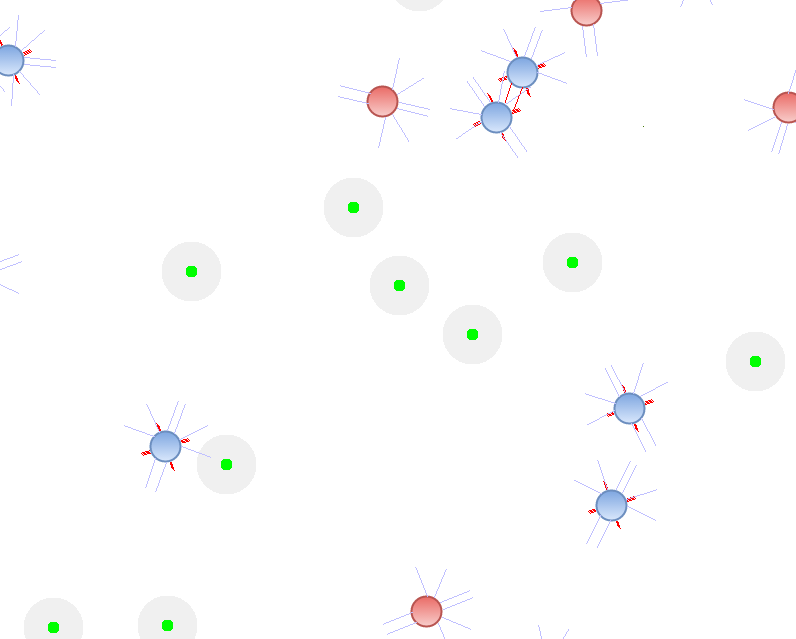
\includegraphics[width=0.65\textwidth]{chapters/res/predator_snippet.png}}
		\caption{A screenshot of a simulation. The predators are marked with red and the robots guided by the evolutionary algorithm are marked with blue}
		\label{fig:predator_screendump}
	\end{figure}

As seen in figure \ref{fig:predator_screendump}, the predators also uses six sensors which they use to decide if they are colliding with an object and what that object is.	
In terms of exploration, the predator controller uses a simple object avoidance tactic.
If the predator robots senses an object on any of its side sensors, it will change its rotational velocity to avoid this object.
In practice, this means that if the predator senses an object on the right, it will steer left, etc.
In the case where there is no collision, a slight random rotational velocity is added such that its movement is more dynamic.
This object avoidance behaviour is always employed as long as it does not sense a robot(prey).
In this case, it will have the opposite behaviour and turn towards the object, as it intends to consume the prey.

In addition to movement, the predators can also consume a robot. 
This happens when there is a collision between a normal robot and a predator robot.
If a robot is consumed, it is removed from the environment and amount of time it stayed alive is recorded for use in the fitness function of the evolutionary algorithm. 
For a predator to be able to eat a robot, the robot must not be part of a robot group of a size less then some configurable threshold.
The reason for this is to give the normal robots some advantage of self-assembling in hopes of potentially evolving this behaviour.  



\subsection{Energy drain}
\subsubsection{Passive}
\subsubsection{Active}
\clearpage
\section{CTRNN}
For this project, an artificial neural network that has gained a lot a popularity in regards to robotics known as Continuous-Time Recurrent Neural Network (CTRNN) was implemented. 
The CTRNN was researched and developed by Randall Beer and adds two new properties to the standard artificial neural network. 
The properties that are introduced in CTRNN is a time constant and a gain.

As most neural networks, the simple integration of the inputs from all neighbouring neurons are added giving us the first standard equation for neural networks:

\begin{equation}
	s_i = \sum_{j=1}^{n}o_{j}w_{i,j}+I_i
\end{equation}
\\
Here, $o_j$ represents the output(after activation) of neuron $j$, $w_{i,j}$ is the weight from neuron $j$ to neuron $i$ and $I_i$ is the sum of all the external inputs to node $i$.

\begin{equation}
\frac{dy_i}{dt} = \frac{1}{\tau_i}[-y_i + s_i + \theta_i]
\end{equation}
\\
In order to preserve the previous state of the ANN, the internal state is stored. 
$y_i$ denotes the internal state of neuron $i$.
To derive the next internal state, Beer computes $\frac{dy_i}{dt}$ as a combination of the next inputs and the current internal state of the node, where a time constant $\tau_i$ decides rate of drain. 
$\theta_i$ is a term added for neuron specific bias, but is only added here for mathematical soundness as it was simply added as a bias node during implementation and hence incorporated in $s_i$.
The time constant $\tau_i$ is what gives CTRNNs the ability to produce rich functionality and convincingly sophisticated cognition.
If $\tau_i$ has a low value then we will have a high degree of drain and hence having the next state being dominated by its new input.
However, if $\tau_i$ has a high value, then we have a higher degree of memory because it will be dominated by its previous state.

\begin{equation}
o_i = \frac{1}{1 + e^{-g_{i}y_{i}}}
\end{equation}
\\
To convert the internal state to an output $o_i$, Beer typically uses sigmoidal activation function.
This is typical in other neural networks as well, but Beer also employs a gain term $g_i$, to influence the activation of the neuron.
\\
\begin{figure}[H]
	\centering
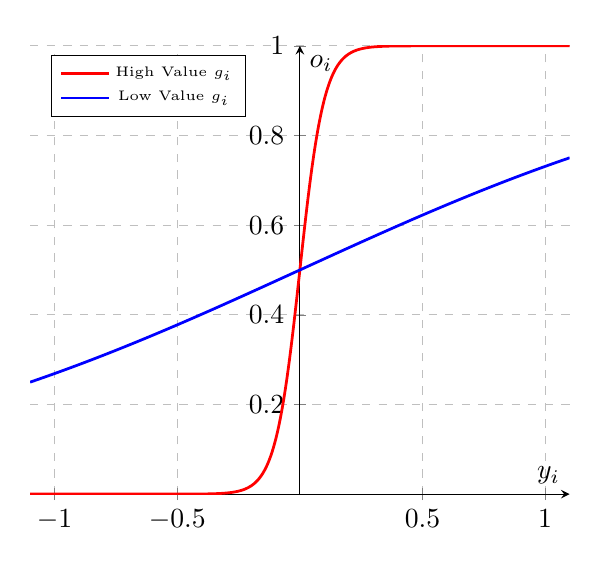
\begin{tikzpicture}
\begin{axis}[
	axis lines = center,
    xlabel = $y_i$,
    ylabel = {$o_i$},
    ymajorgrids=true,
    xmajorgrids=true,
    grid style=dashed,
    legend style={at={(0.22, 0.98)},anchor=north, font=\tiny}
]
%Below the red parabola is defined
\addplot [
    domain=-1.1:1.1, 
    samples=500, 
    color=red,
    line width=1pt,
]
{1/(1+e^(-20*x)};
\addlegendentry{High Value $g_i$}
%Here the blue parabloa is defined
\addplot [
    domain=-1.1:1.1, 
    samples=100, 
    color=blue,
	line width=1pt,
]
{1/(1+e^(-1*x)};
\addlegendentry{Low Value $g_i$}
 
\end{axis}
\end{tikzpicture}
	\caption{The difference in the activation function with respect to $y_i$ based on a low and high value of $g_i$}
	\label{CTRNN-gGraph}
\end{figure}

As seen in figure \ref{CTRNN-gGraph}, the value of the gain parameter can influence the activation function in such a way that it can be a smooth, almost linear, function or it can take on the behaviour of an activation function resembling a switch.
Having the ability to change the activation function on a neuron to neuron basis, is the second reason(the first being time constants) CTRNNs can give rise to complex and rich behaviour.



	\subsection{Drain}
	\subsection{Activation function}
	\subsection{Topologies}
		\subsubsection{Dense}
		\subsubsection{Sparse}
\clearpage
\section{Evolutionary algorithm}
	\subsection{Genotype}
	\subsection{Initialization}
	\subsection{Mutation operators}
		\subsubsection{Random}
		\subsubsection{Incremental}
	\subsection{Selection mechanism}
	The selection step of an evolutionary algorithm is responsible for selecting which individuals should become parents.
	In other words, it applies selection pressure.
	If the selection pressure is too high the algorithm may converge prematurely, and if it is too low the search may take more time than necessary.
	For the experiment two different selection mechanisms have been implemented.
		\subsubsection{Proportional selection}
		In this selection scheme individuals are selected for reproduction with a probability proportional to their fitness compared to the total fitness in the population.
		It is common to apply a scaling function on the fitness in the population to adjust selection pressure.
		A scaling function that is often used with proportional selection is \emph{Sigma scaling}\cite{goh_sexual_2003}:
		\begin{equation}
		S(f, \overline{f}, \sigma, s) = s + \frac{f - \overline{f} }{2\sigma}
		\end{equation}
		
		where \emph{f} is the fitness of an individual, $\overline{f}$ is the mean fitness of the generation, $\sigma$ is the fitness variance, and \emph{s} is a scaling factor that can be used to adjust the selection pressure.
		
		Sigma scaling modifies the selection pressure introduced in the raw fitness by using the populations fitness variance as a scaling factor.
		This has the effect of dampening the selection pressure when there are a few individuals with an exceedingly higher fitness than the rest, and increasing the selection pressure when the population has a low variance.
		
		The values obtained from the scaling can now be used to select parents by sampling the distribution.
		\emph{Roulette wheel selection}(RWS)\cite{goh_sexual_2003}  is one such method.
		RWS can be visualized as giving each potential parent a sector with size relative to the scaled fitness in the roulette wheel(figure \ref{fig:roulette}).
		The parents are then selected by spinning the wheel until the desired number of parents are picked.
		
		\begin{figure}[H]
			
			\centering
			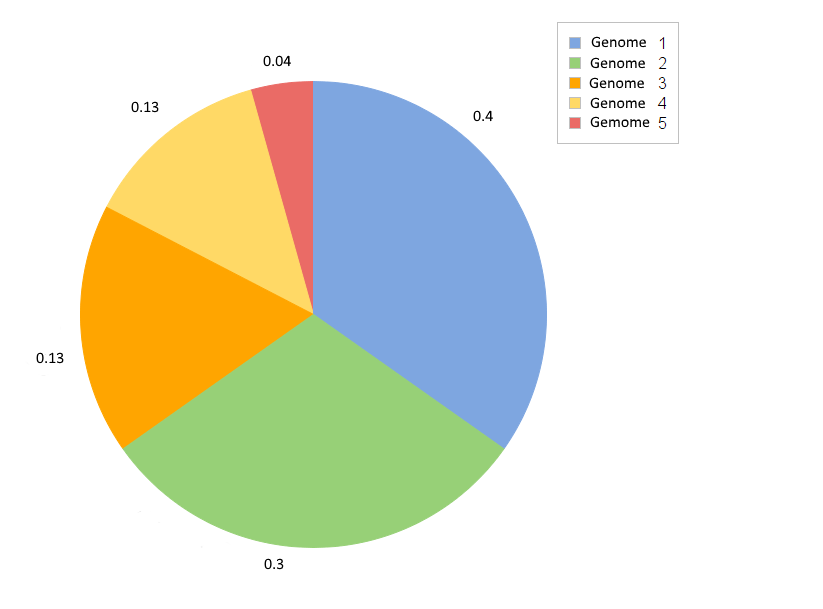
\includegraphics[width=0.80\textwidth, clip]{chapters/res/roulette.png}
			\caption{A roulette wheel where the size of each sector represents the probability of picking a particular parent.}
			\label{fig:roulette}
		\end{figure}
		
		\subsubsection{Tournament selection}
		In contrast to proportional selection the individuals do not compete with the entire population, but instead compete within groups selected at random.
		Tournament selection performs parent selection by picking individuals at random into a group.
		From the group the fittest individual is selected as the parent.
		This process is repeated until the desired number of parents have been selected.
		The group size varies between implementations, but typical implementations compare two\cite{goh_sexual_2003} individuals at a time, depicted in figure \ref{fig:tournament}
		
				\begin{figure}[H]
					
					\centering
					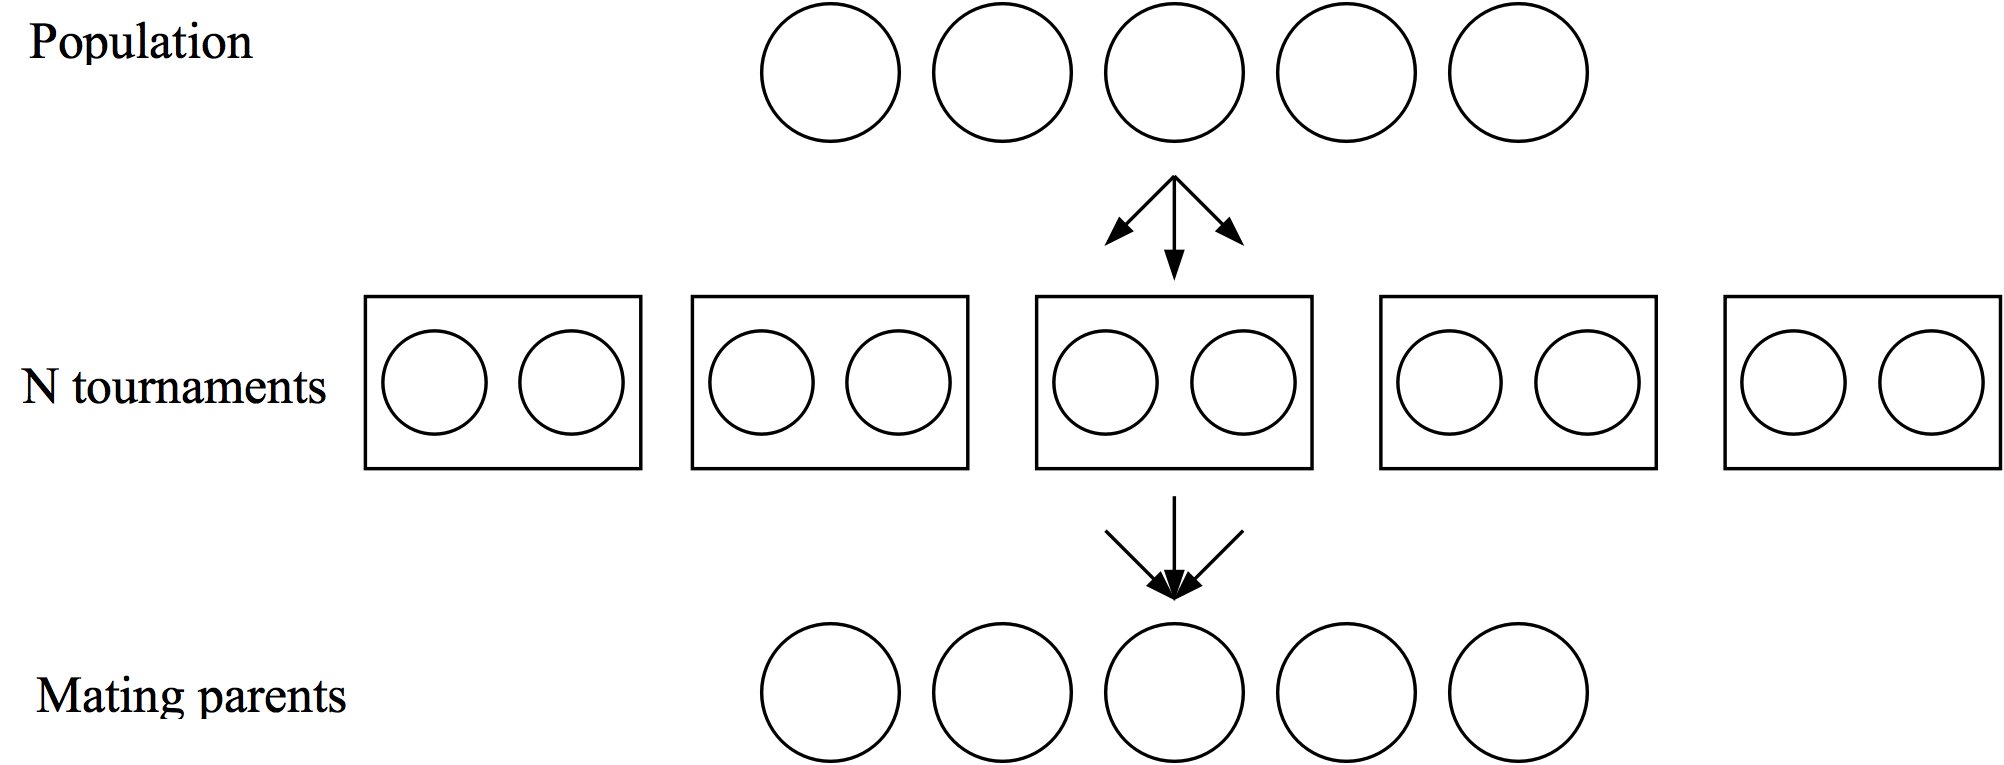
\includegraphics[width=\textwidth, clip]{chapters/res/Tournament.png}
					\caption{Selecting parents using a binary tournament.}
					\label{fig:tournament}
				\end{figure}
		The described process introduces a high selection pressure since it selects the fittest individual from each group.
		It is common to include an acceptance threshold, $t$, into the selection to modify the selection pressure\cite{goh_sexual_2003}.
		Each time an individual is to be selected a random number $r \in (0, 1)$, is generated.
		If $r < t$, then the fittest individual is chosen, otherwise the less fit individual is chosen. The selection pressure can then be tuned by increasing or decreasing the acceptance threshold. A lower value for $t$ decreases the selection pressure, while a higher value increases the selection pressure.
		
\clearpage
\section{Data gathering}
	\section{Loggers}
	\section{Analysis}
\clearpage
\subsection{Extras/Appendix?}
	\subsection{Parallelization}
	\subsection{Python graph tool}
	\subsection{System configuration}
\clearpage
	
\clearpage

\chapter{Results and Discussion}
\label{ch:results_and_discussion}
This chapter shows the results of the simulations done with the framework shown in ch. \ref{ch:methodology} as well as discussing the results.
The chapter is mainly divided into two sections, the first explaining the configuration of the simulation as well as results depicted by graph-data.
The second section focuses on discussing the results in terms of the reason they have certain values and graphs, as well as a comparison between the different simulations and discovery of correlations and behavioural similarities.

\section{Experimental Results}
As stated in the chapter introduction, this section covers the results of the simulations. 
Even though the simulator supports a wide variety of different configurations, three main simulation groups chosen for this particular study.
The first group considers different connection port configurations for the robots.
The second simulation group varies the environment that the robots spend their life time in.
The third and final simulation group aims to observe the affect of local communication between the robots in a self-assembly structure(the implementation is shown in sec. \ref{sec:local_comm}).
The two first simulation groups targets to contribute to the three main self-assembly mechanisms discussed in ch. \ref{ch:background}(Self-assembly Architectures, Hardware Mechanisms and Assembly Protocols).
The local communication simulation group aims to study the affect giving the robots the ability to perform simple communication between the robots in a group.

\subsection{Port Configuration}
The first group of simulations that were done was varying the number of connection ports of the robots and their configuration.
These simulations where done such that one could record and discuss the impact of connections between the robots.
In more detail, this group of experiments where conducted such that one could record:

\begin{itemize}
	\item How the number of ports affected the general performance of the system based on the number of ports.
	\item If there is any noticeable difference in the self-assembly architecture.
	\item In what way the port configuration promotes self-assembly, both in therms of the sizes of the different robot groups, and the number of groups.
	\item How the port configuration affect the fitness of the experiment, in terms of convergence and final result.
\end{itemize}

The goal of running these simulations is to make correlations between its results to show how configuring the hardware mechanism can affect a self-assembly system.
 
For this group of simulations, the most relevant statistics will be the difference between group actions versus single robot actions.
The following pages show the recorded data for simulations using, 2 connection ports, 3 connection ports and 4 connection ports.


\begin{figure}[H]
	\centering
	\begin{subfigure}[b]{0.31\textwidth}
		\centering
		\fbox{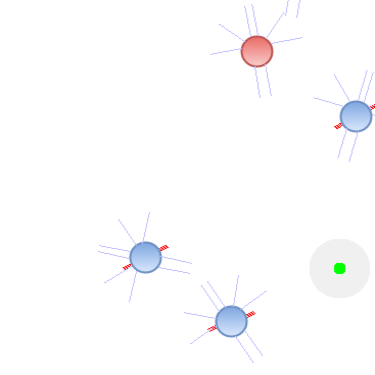
\includegraphics[height=\linewidth]{chapters/res/2-conn.png}}
		\caption{2-ports}
	\end{subfigure}
	\begin{subfigure}[b]{0.31\textwidth}
		\centering
		\fbox{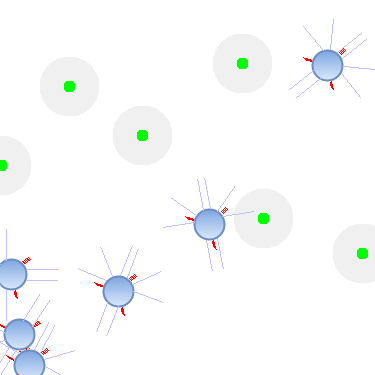
\includegraphics[height=\linewidth]{chapters/res/3-conn.png}}
		\caption{3-ports}
	\end{subfigure}
	\begin{subfigure}[b]{0.31\textwidth}
		\centering
		\fbox{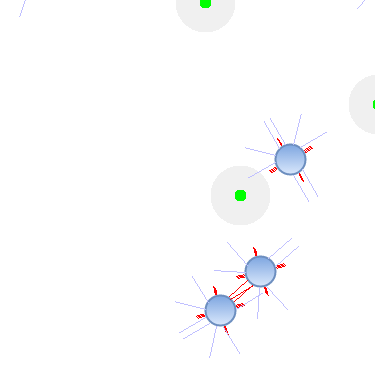
\includegraphics[height=\linewidth]{chapters/res/4-conn.png}}
		\caption{4-ports}
	\end{subfigure}
	\caption{The three different port configurations used in simulation}
	\label{fig:collective-behaviour}
\end{figure}


Common configuration parameters of importance for the simulations are listed in table[x].

\begin{table}[H]
	\centering
	\label{tab-environment}
	\begin{tabular}{|c|c|}
		\hline Parameter & Value \\ 
		\hline Number of Robots & 20 \\ 
		\hline Iterations per Generation & 10000 \\
		\hline Scenarios & 3 \\ 
		\hline Generations & 150 \\ 
		\hline 
		
	\end{tabular} 
	\caption{The simulation parameters for the environments.}
\end{table}



\newpage
\pagestyle{plain}

\vspace*{-2.0cm}
\textbf{\Huge LARGE SAMPLE HEADER}
\vspace{1.5cm}
\begin{tikzpicture}[remember picture,overlay]
   \node[anchor=south east,inner sep=20pt] at (current page.south east)
              {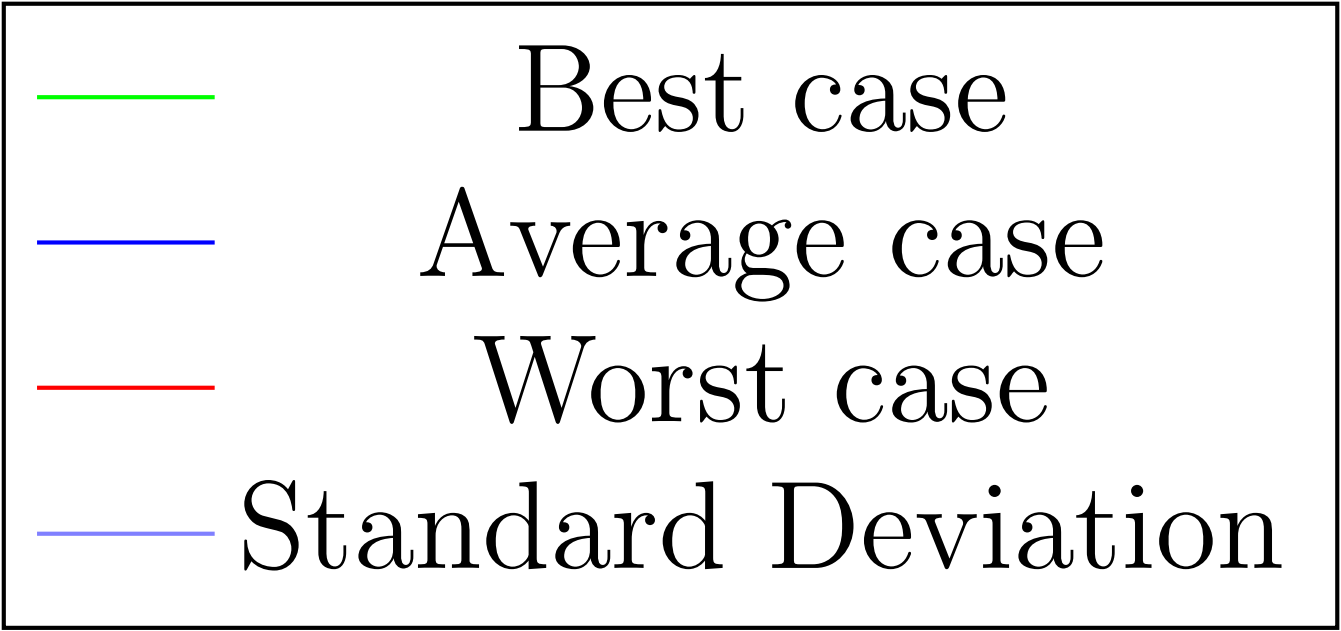
\includegraphics[scale=0.1]{chapters/res/generated_graph_legend.png}};
\end{tikzpicture}

\begin{figure}[H]
\vspace*{-1cm}
	\makebox[\linewidth][c]{%
	\begin{subfigure}[b]{0.7\textwidth}
		\centering
		\resizebox{0.9\linewidth}{!}{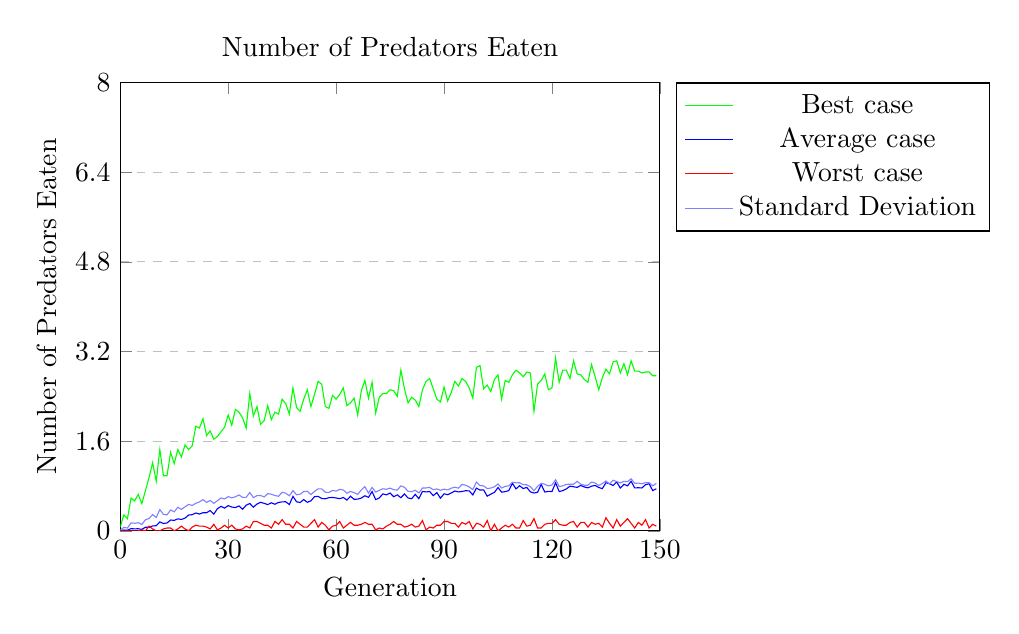
\begin{tikzpicture}
\begin{axis}[
	title={Number of Predators Eaten},
	xlabel={Generation},
	ylabel={Number of Predators Eaten},
	xmin=0, xmax=150,
	ymin=0, ymax=8,
	xtick={0.0,30.0,60.0,90.0,120.0,150.0},
	ytick={0.0,1.6,3.2,4.800000000000001,6.4,8.0},
	legend pos=outer north east,
	ymajorgrids=true,
	grid style=dashed,
]

\addplot[
	color=green,
	]
	coordinates {
	(0,0.06666666666666667)(1,0.2833333333333334)(2,0.21666666666666667)(3,0.5833333333333333)(4,0.5333333333333333)(5,0.65)(6,0.48333333333333334)(7,0.7166666666666668)(8,0.95)(9,1.2166666666666668)(10,0.8833333333333335)(11,1.4500000000000004)(12,0.9833333333333334)(13,0.9833333333333335)(14,1.4000000000000001)(15,1.2)(16,1.45)(17,1.3166666666666669)(18,1.5333333333333339)(19,1.4500000000000002)(20,1.5166666666666666)(21,1.8666666666666667)(22,1.8333333333333335)(23,2.0000000000000004)(24,1.7)(25,1.7833333333333334)(26,1.633333333333333)(27,1.6833333333333333)(28,1.7666666666666673)(29,1.8500000000000003)(30,2.066666666666667)(31,1.8833333333333335)(32,2.1666666666666674)(33,2.116666666666667)(34,2.0166666666666666)(35,1.8333333333333337)(36,2.45)(37,2.0500000000000003)(38,2.2166666666666672)(39,1.9)(40,1.9666666666666668)(41,2.2333333333333334)(42,1.9833333333333334)(43,2.1166666666666667)(44,2.083333333333333)(45,2.35)(46,2.266666666666667)(47,2.0833333333333335)(48,2.5500000000000003)(49,2.2)(50,2.1333333333333333)(51,2.35)(52,2.516666666666666)(53,2.2166666666666663)(54,2.4333333333333327)(55,2.6666666666666665)(56,2.6166666666666667)(57,2.2166666666666663)(58,2.1833333333333336)(59,2.416666666666667)(60,2.35)(61,2.4333333333333336)(62,2.5500000000000003)(63,2.233333333333334)(64,2.283333333333333)(65,2.3666666666666667)(66,2.066666666666667)(67,2.5)(68,2.683333333333334)(69,2.3666666666666667)(70,2.6500000000000004)(71,2.1)(72,2.3833333333333337)(73,2.45)(74,2.4499999999999997)(75,2.5166666666666666)(76,2.5)(77,2.3999999999999995)(78,2.8666666666666663)(79,2.533333333333333)(80,2.2833333333333337)(81,2.383333333333333)(82,2.3333333333333335)(83,2.216666666666667)(84,2.5166666666666675)(85,2.6666666666666665)(86,2.716666666666667)(87,2.533333333333333)(88,2.3500000000000005)(89,2.3000000000000007)(90,2.5666666666666673)(91,2.316666666666667)(92,2.4666666666666663)(93,2.6666666666666665)(94,2.5833333333333335)(95,2.716666666666667)(96,2.6666666666666665)(97,2.5500000000000003)(98,2.3666666666666667)(99,2.9166666666666665)(100,2.95)(101,2.5333333333333337)(102,2.5999999999999996)(103,2.483333333333334)(104,2.7)(105,2.7833333333333328)(106,2.35)(107,2.6833333333333336)(108,2.6499999999999995)(109,2.7833333333333337)(110,2.8666666666666667)(111,2.816666666666667)(112,2.75)(113,2.833333333333334)(114,2.8166666666666664)(115,2.133333333333333)(116,2.6166666666666667)(117,2.683333333333333)(118,2.8)(119,2.5166666666666666)(120,2.55)(121,3.083333333333333)(122,2.6500000000000004)(123,2.866666666666667)(124,2.866666666666667)(125,2.716666666666667)(126,3.033333333333333)(127,2.8)(128,2.7833333333333337)(129,2.6999999999999997)(130,2.65)(131,2.966666666666666)(132,2.75)(133,2.5166666666666666)(134,2.7333333333333334)(135,2.8833333333333324)(136,2.8000000000000003)(137,3.016666666666667)(138,3.0333333333333323)(139,2.8166666666666673)(140,2.983333333333333)(141,2.783333333333333)(142,3.0333333333333328)(143,2.8499999999999996)(144,2.8499999999999996)(145,2.8166666666666673)(146,2.8333333333333335)(147,2.833333333333334)(148,2.766666666666667)(149,2.7666666666666666)
	};
	\addlegendentry{Best case}
\addplot[
	color=blue,
	]
	coordinates {
	(0,0.0027777777777777775)(1,0.014583333333333334)(2,0.010416666666666666)(3,0.03888888888888888)(4,0.03472222222222222)(5,0.03680555555555555)(6,0.025694444444444443)(7,0.06319444444444446)(8,0.062499999999999986)(9,0.08750000000000001)(10,0.0909722222222222)(11,0.15833333333333335)(12,0.13055555555555554)(13,0.14027777777777778)(14,0.1930555555555556)(15,0.1861111111111111)(16,0.21319444444444444)(17,0.20347222222222222)(18,0.2263888888888889)(19,0.2819444444444444)(20,0.28819444444444436)(21,0.31805555555555554)(22,0.2993055555555556)(23,0.3229166666666668)(24,0.32291666666666663)(25,0.3625)(26,0.29861111111111105)(27,0.39375)(28,0.43680555555555545)(29,0.4048611111111111)(30,0.45)(31,0.4243055555555556)(32,0.4152777777777778)(33,0.44375)(34,0.38472222222222224)(35,0.45625000000000004)(36,0.48749999999999993)(37,0.4208333333333332)(38,0.4777777777777778)(39,0.5083333333333332)(40,0.4902777777777778)(41,0.4673611111111111)(42,0.5)(43,0.47361111111111104)(44,0.5062500000000001)(45,0.517361111111111)(46,0.5180555555555556)(47,0.46805555555555556)(48,0.6145833333333334)(49,0.5187499999999998)(50,0.5048611111111111)(51,0.5576388888888888)(52,0.5090277777777777)(53,0.5347222222222222)(54,0.6097222222222222)(55,0.6145833333333333)(56,0.5763888888888887)(57,0.5722222222222222)(58,0.5909722222222223)(59,0.5958333333333333)(60,0.586111111111111)(61,0.5736111111111111)(62,0.5944444444444444)(63,0.548611111111111)(64,0.617361111111111)(65,0.5625000000000001)(66,0.5652777777777778)(67,0.5847222222222223)(68,0.6256944444444443)(69,0.5972222222222222)(70,0.7013888888888888)(71,0.5562499999999999)(72,0.5874999999999999)(73,0.6590277777777778)(74,0.6409722222222222)(75,0.6743055555555557)(76,0.6090277777777776)(77,0.6416666666666666)(78,0.5909722222222223)(79,0.6576388888888888)(80,0.5854166666666666)(81,0.5722222222222222)(82,0.6506944444444446)(83,0.5729166666666667)(84,0.7020833333333334)(85,0.6944444444444444)(86,0.7006944444444444)(87,0.627777777777778)(88,0.6819444444444445)(89,0.5819444444444444)(90,0.6604166666666667)(91,0.6444444444444444)(92,0.675)(93,0.7104166666666666)(94,0.6937499999999999)(95,0.7020833333333333)(96,0.7152777777777778)(97,0.7125000000000001)(98,0.640277777777778)(99,0.7618055555555556)(100,0.7270833333333332)(101,0.7305555555555555)(102,0.6180555555555556)(103,0.654861111111111)(104,0.6847222222222221)(105,0.7729166666666666)(106,0.6895833333333333)(107,0.6999999999999998)(108,0.717361111111111)(109,0.8486111111111111)(110,0.7479166666666666)(111,0.8048611111111111)(112,0.7541666666666665)(113,0.7743055555555556)(114,0.6958333333333333)(115,0.6743055555555554)(116,0.6875)(117,0.8270833333333334)(118,0.6916666666666668)(119,0.7041666666666667)(120,0.7000000000000001)(121,0.8569444444444445)(122,0.7013888888888891)(123,0.7166666666666666)(124,0.7486111111111111)(125,0.7965277777777778)(126,0.786111111111111)(127,0.775)(128,0.8097222222222221)(129,0.7826388888888891)(130,0.7666666666666667)(131,0.7972222222222225)(132,0.8090277777777779)(133,0.7736111111111111)(134,0.7520833333333333)(135,0.8583333333333333)(136,0.8416666666666668)(137,0.8090277777777779)(138,0.8715277777777779)(139,0.7624999999999998)(140,0.8298611111111112)(141,0.8020833333333335)(142,0.8840277777777777)(143,0.7652777777777777)(144,0.76875)(145,0.7645833333333333)(146,0.8222222222222222)(147,0.8402777777777778)(148,0.7180555555555557)(149,0.7500000000000001)
	};
	\addlegendentry{Average case}
\addplot[
	color=red,
	]
	coordinates {
	(0,0.0)(1,0.0)(2,0.0)(3,0.0)(4,0.0)(5,0.0)(6,0.016666666666666666)(7,0.0)(8,0.08333333333333334)(9,0.03333333333333333)(10,0.0)(11,0.0)(12,0.03333333333333333)(13,0.05)(14,0.05)(15,0.0)(16,0.03333333333333333)(17,0.08333333333333334)(18,0.03333333333333333)(19,0.0)(20,0.06666666666666667)(21,0.09999999999999999)(22,0.08333333333333333)(23,0.08333333333333333)(24,0.06666666666666667)(25,0.03333333333333333)(26,0.11666666666666667)(27,0.016666666666666666)(28,0.05)(29,0.1)(30,0.05)(31,0.1)(32,0.03333333333333333)(33,0.016666666666666666)(34,0.03333333333333333)(35,0.08333333333333334)(36,0.05)(37,0.16666666666666666)(38,0.16666666666666666)(39,0.13333333333333333)(40,0.1)(41,0.1)(42,0.05)(43,0.16666666666666666)(44,0.11666666666666667)(45,0.19999999999999998)(46,0.11666666666666667)(47,0.11666666666666667)(48,0.05)(49,0.16666666666666666)(50,0.11666666666666667)(51,0.06666666666666667)(52,0.06666666666666667)(53,0.13333333333333333)(54,0.19999999999999998)(55,0.06666666666666667)(56,0.15)(57,0.09999999999999999)(58,0.016666666666666666)(59,0.08333333333333334)(60,0.1)(61,0.16666666666666666)(62,0.05)(63,0.1)(64,0.15)(65,0.1)(66,0.1)(67,0.11666666666666667)(68,0.15)(69,0.11666666666666667)(70,0.11666666666666667)(71,0.016666666666666666)(72,0.05)(73,0.03333333333333333)(74,0.08333333333333333)(75,0.11666666666666665)(76,0.16666666666666666)(77,0.11666666666666667)(78,0.11666666666666667)(79,0.06666666666666667)(80,0.08333333333333333)(81,0.11666666666666667)(82,0.06666666666666667)(83,0.08333333333333333)(84,0.18333333333333332)(85,0.016666666666666666)(86,0.06666666666666667)(87,0.05)(88,0.1)(89,0.1)(90,0.16666666666666666)(91,0.16666666666666666)(92,0.13333333333333333)(93,0.13333333333333333)(94,0.06666666666666667)(95,0.15)(96,0.11666666666666667)(97,0.16666666666666666)(98,0.03333333333333333)(99,0.13333333333333333)(100,0.11666666666666667)(101,0.06666666666666667)(102,0.18333333333333332)(103,0.0)(104,0.11666666666666667)(105,0.0)(106,0.05)(107,0.1)(108,0.06666666666666667)(109,0.11666666666666667)(110,0.05)(111,0.05)(112,0.18333333333333332)(113,0.08333333333333333)(114,0.1)(115,0.21666666666666665)(116,0.05)(117,0.05)(118,0.11666666666666667)(119,0.13333333333333333)(120,0.13333333333333333)(121,0.19999999999999998)(122,0.11666666666666667)(123,0.1)(124,0.1)(125,0.15)(126,0.16666666666666666)(127,0.06666666666666667)(128,0.15)(129,0.15)(130,0.06666666666666667)(131,0.15)(132,0.11666666666666667)(133,0.13333333333333333)(134,0.06666666666666667)(135,0.2333333333333333)(136,0.13333333333333333)(137,0.05)(138,0.19999999999999998)(139,0.08333333333333334)(140,0.15)(141,0.21666666666666665)(142,0.13333333333333333)(143,0.05)(144,0.15)(145,0.1)(146,0.19999999999999998)(147,0.05)(148,0.11666666666666667)(149,0.08333333333333334)
	};
	\addlegendentry{Worst case}
\addplot[
	color=blue!50,
	]
	coordinates {
	(0,0.013321754231424222)(1,0.060833289362768106)(2,0.04995657836784083)(3,0.1419770493918252)(4,0.13501238835938728)(5,0.1442871196495461)(6,0.11204068334010286)(7,0.19714417226441955)(8,0.21960991755978337)(9,0.28968486977098945)(10,0.238687514679114)(11,0.3786918693113443)(12,0.2935448600032916)(13,0.2844952984387647)(14,0.372511545259369)(15,0.33879024291337473)(16,0.4206592613842742)(17,0.38257320635094777)(18,0.42771509133577684)(19,0.4716223129461485)(20,0.4520067717329728)(21,0.4909602764965256)(22,0.5161763337308514)(23,0.5564735513432749)(24,0.5060492604704913)(25,0.5422436063745897)(26,0.48963719621083973)(27,0.5359339105518787)(28,0.5860066363926782)(29,0.5693568786187266)(30,0.6099192082544038)(31,0.5882238317566547)(32,0.607857088494673)(33,0.6394546683219003)(34,0.5970339837409993)(35,0.5972632411779724)(36,0.68322083148292)(37,0.5916614833187916)(38,0.6280708404141233)(39,0.6299428343819048)(40,0.6056271281654441)(41,0.6639054614712624)(42,0.6528687871597612)(43,0.6295717033514034)(44,0.616229759889133)(45,0.689657756805591)(46,0.6699016992879209)(47,0.6250124623986605)(48,0.7180117907369525)(49,0.6435944039967669)(50,0.6521647898488324)(51,0.7008041446690075)(52,0.7059741615880475)(53,0.6465514312525087)(54,0.7038809180614064)(55,0.7493456799062804)(56,0.7494401726922688)(57,0.6876540411026748)(58,0.68466013418382)(59,0.7212129247033078)(60,0.7092208330782678)(61,0.7389405641680545)(62,0.7289289504830331)(63,0.6714966656671288)(64,0.7018397381768663)(65,0.6815984912044807)(66,0.6497540522563912)(67,0.7283995821663413)(68,0.7882004878794159)(69,0.6724042390361087)(70,0.7746798131373714)(71,0.6912916309640261)(72,0.7229842206808591)(73,0.7503699249210067)(74,0.7407622530323247)(75,0.7615677520196351)(76,0.7345674694007291)(77,0.7266216615005409)(78,0.8015375958267322)(79,0.7766789813634328)(80,0.7054858278385088)(81,0.6977940903238453)(82,0.7237714535795581)(83,0.6761884688106625)(84,0.7635855802061089)(85,0.7650218922339868)(86,0.7746595096923177)(87,0.7332585277989179)(88,0.7481283741054381)(89,0.7237771304816039)(90,0.7432408988498297)(91,0.7298345279364067)(92,0.7604266773106071)(93,0.7790426686573553)(94,0.7606797099685648)(95,0.8271537135997328)(96,0.8139945560474893)(97,0.783426893567695)(98,0.7350243151901092)(99,0.8709183203828984)(100,0.8066295336685159)(101,0.8021588574757975)(102,0.7529733412280979)(103,0.7630882413250057)(104,0.7853713050243827)(105,0.8363310889304815)(106,0.7629301988983602)(107,0.7931436318334675)(108,0.801764491886245)(109,0.8664327265828317)(110,0.8558387169473423)(111,0.8581239686450739)(112,0.8238387648770378)(113,0.821229304500997)(114,0.789196975573271)(115,0.715351203584567)(116,0.7940016366448526)(117,0.8464841204694811)(118,0.8307797969259251)(119,0.8013506513486762)(120,0.817602304998275)(121,0.9129448648573786)(122,0.7905121674637492)(123,0.8021628031598314)(124,0.8285660559882189)(125,0.8319423484917443)(126,0.8315605951626273)(127,0.882474226661018)(128,0.8320387001836311)(129,0.8139549192729018)(130,0.8139178481681871)(131,0.870689062049016)(132,0.8529359611434546)(133,0.8101647386169293)(134,0.8431190054454514)(135,0.8899150638120932)(136,0.8354590298630876)(137,0.9023553608745827)(138,0.8790385053002011)(139,0.85472658237739)(140,0.8833561755440055)(141,0.8768583978509924)(142,0.9275683535122932)(143,0.8468787053700149)(144,0.8517028853522297)(145,0.8396018401686776)(146,0.8600484378160977)(147,0.8595326889077773)(148,0.8026347338932457)(149,0.8464698767347983)
	};
	\addlegendentry{Standard Deviation}
\end{axis}
\end{tikzpicture}
}
		\caption{Some sample caption}
	\end{subfigure}%
	\begin{subfigure}[b]{0.7\textwidth}	
		\centering
		\resizebox{0.9\linewidth}{!}{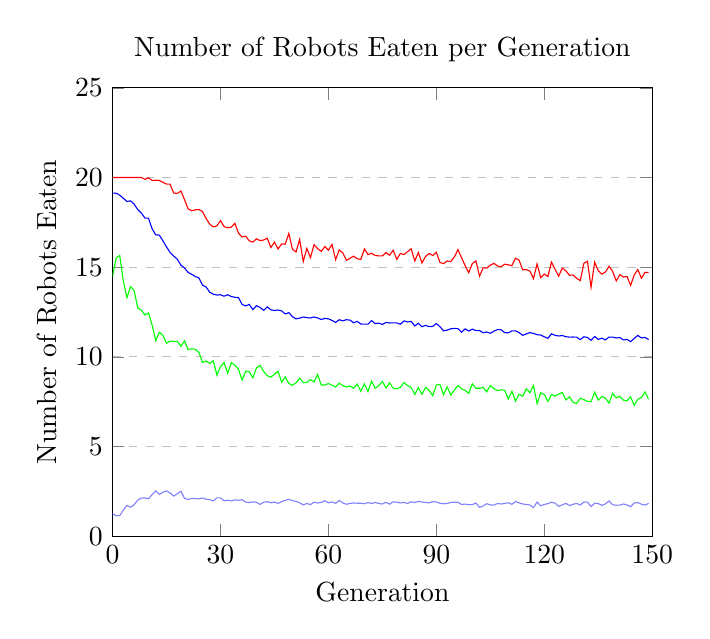
\begin{tikzpicture}
\begin{axis}[
	title={Number of Robots Eaten per Generation},
	xlabel={Generation},
	ylabel={Number of Robots Eaten},
	xmin=0, xmax=150,
	ymin=0, ymax=25,
	xtick={0.0,30.0,60.0,90.0,120.0,150.0},
	ytick={0.0,5.0,10.0,15.0,20.0,25.0},
	ymajorgrids=true,
	grid style=dashed,
]

\addplot[
	color=red,
	]
	coordinates {
	(0,20.0)(1,20.0)(2,20.0)(3,20.0)(4,20.0)(5,20.0)(6,20.0)(7,20.0)(8,20.0)(9,19.9)(10,19.983333333333334)(11,19.833333333333336)(12,19.85)(13,19.833333333333332)(14,19.73333333333333)(15,19.633333333333333)(16,19.63333333333333)(17,19.133333333333333)(18,19.116666666666664)(19,19.249999999999993)(20,18.766666666666662)(21,18.249999999999996)(22,18.150000000000002)(23,18.2)(24,18.216666666666665)(25,18.099999999999998)(26,17.716666666666665)(27,17.4)(28,17.25)(29,17.3)(30,17.6)(31,17.266666666666662)(32,17.200000000000003)(33,17.233333333333334)(34,17.45)(35,16.9)(36,16.683333333333334)(37,16.733333333333334)(38,16.466666666666665)(39,16.400000000000002)(40,16.583333333333332)(41,16.48333333333333)(42,16.516666666666666)(43,16.616666666666667)(44,16.1)(45,16.4)(46,16.01666666666667)(47,16.3)(48,16.28333333333333)(49,16.883333333333333)(50,16.0)(51,15.85)(52,16.55)(53,15.316666666666666)(54,16.049999999999997)(55,15.533333333333335)(56,16.25)(57,16.033333333333335)(58,15.883333333333333)(59,16.150000000000002)(60,15.950000000000003)(61,16.266666666666666)(62,15.416666666666668)(63,15.966666666666667)(64,15.8)(65,15.383333333333335)(66,15.5)(67,15.616666666666665)(68,15.466666666666667)(69,15.433333333333337)(70,16.016666666666666)(71,15.700000000000001)(72,15.783333333333331)(73,15.650000000000002)(74,15.633333333333335)(75,15.633333333333335)(76,15.816666666666668)(77,15.666666666666664)(78,15.950000000000001)(79,15.433333333333332)(80,15.766666666666667)(81,15.700000000000003)(82,15.866666666666667)(83,16.03333333333333)(84,15.35)(85,15.816666666666665)(86,15.233333333333334)(87,15.599999999999998)(88,15.766666666666664)(89,15.649999999999999)(90,15.833333333333332)(91,15.266666666666666)(92,15.2)(93,15.350000000000001)(94,15.316666666666668)(95,15.566666666666665)(96,15.983333333333334)(97,15.533333333333331)(98,15.083333333333334)(99,14.700000000000001)(100,15.200000000000001)(101,15.35)(102,14.499999999999998)(103,14.966666666666667)(104,14.95)(105,15.116666666666667)(106,15.216666666666669)(107,15.066666666666666)(108,15.033333333333335)(109,15.166666666666666)(110,15.133333333333333)(111,15.083333333333334)(112,15.499999999999998)(113,15.383333333333335)(114,14.85)(115,14.866666666666664)(116,14.783333333333331)(117,14.366666666666669)(118,15.183333333333335)(119,14.416666666666666)(120,14.616666666666665)(121,14.483333333333336)(122,15.283333333333331)(123,14.883333333333333)(124,14.5)(125,14.950000000000001)(126,14.799999999999999)(127,14.549999999999999)(128,14.566666666666668)(129,14.383333333333331)(130,14.249999999999998)(131,15.216666666666669)(132,15.333333333333332)(133,13.883333333333335)(134,15.283333333333331)(135,14.799999999999999)(136,14.61666666666667)(137,14.733333333333336)(138,15.049999999999999)(139,14.766666666666666)(140,14.233333333333334)(141,14.583333333333334)(142,14.45)(143,14.483333333333334)(144,13.983333333333333)(145,14.566666666666666)(146,14.866666666666667)(147,14.383333333333333)(148,14.716666666666665)(149,14.699999999999996)
	};
\addplot[
	color=blue,
	]
	coordinates {
	(0,19.136111111111113)(1,19.124305555555555)(2,19.017361111111107)(3,18.839583333333334)(4,18.666666666666664)(5,18.7)(6,18.51875)(7,18.213194444444447)(8,18.021527777777777)(9,17.740972222222222)(10,17.73263888888889)(11,17.135416666666668)(12,16.80277777777778)(13,16.788888888888888)(14,16.469444444444445)(15,16.130555555555556)(16,15.822916666666663)(17,15.620138888888889)(18,15.444444444444446)(19,15.112499999999997)(20,14.956944444444444)(21,14.710416666666669)(22,14.604166666666668)(23,14.48194444444444)(24,14.404166666666667)(25,13.99513888888889)(26,13.897222222222226)(27,13.60625)(28,13.49375)(29,13.445833333333335)(30,13.464583333333334)(31,13.382638888888886)(32,13.465277777777779)(33,13.362499999999999)(34,13.322222222222223)(35,13.304861111111112)(36,12.925694444444447)(37,12.840972222222225)(38,12.92638888888889)(39,12.63472222222222)(40,12.853472222222221)(41,12.758333333333333)(42,12.593055555555557)(43,12.7875)(44,12.625)(45,12.584722222222224)(46,12.614583333333334)(47,12.563888888888888)(48,12.394444444444444)(49,12.468055555555555)(50,12.236111111111114)(51,12.121527777777779)(52,12.160416666666668)(53,12.220138888888886)(54,12.186805555555557)(55,12.167361111111113)(56,12.224305555555556)(57,12.17083333333333)(58,12.08333333333333)(59,12.14513888888889)(60,12.119444444444444)(61,12.034722222222223)(62,11.922916666666667)(63,12.070138888888888)(64,12.0125)(65,12.070833333333335)(66,12.050694444444446)(67,11.902083333333335)(68,11.979861111111113)(69,11.831944444444444)(70,11.825000000000001)(71,11.822222222222226)(72,12.022916666666669)(73,11.853472222222223)(74,11.881250000000001)(75,11.806944444444447)(76,11.919444444444444)(77,11.890277777777776)(78,11.897222222222226)(79,11.896527777777777)(80,11.815972222222225)(81,12.005555555555556)(82,11.944444444444446)(83,11.979166666666666)(84,11.726388888888891)(85,11.872916666666665)(86,11.680555555555555)(87,11.754861111111106)(88,11.683333333333332)(89,11.70277777777778)(90,11.859722222222222)(91,11.681944444444444)(92,11.451388888888888)(93,11.489583333333334)(94,11.565277777777778)(95,11.58611111111111)(96,11.573611111111111)(97,11.375000000000004)(98,11.55902777777778)(99,11.440277777777778)(100,11.547916666666666)(101,11.461805555555555)(102,11.468750000000002)(103,11.348611111111111)(104,11.386111111111111)(105,11.315972222222223)(106,11.430555555555554)(107,11.523611111111109)(108,11.515277777777778)(109,11.349305555555553)(110,11.340277777777779)(111,11.447916666666668)(112,11.45347222222222)(113,11.354166666666666)(114,11.200000000000005)(115,11.280555555555553)(116,11.352777777777778)(117,11.306944444444444)(118,11.238194444444442)(119,11.21527777777778)(120,11.120138888888889)(121,11.032638888888888)(122,11.284722222222223)(123,11.200694444444443)(124,11.163194444444445)(125,11.189583333333331)(126,11.125694444444445)(127,11.101388888888888)(128,11.10625)(129,11.09861111111111)(130,10.959722222222222)(131,11.120138888888887)(132,11.081944444444444)(133,10.925)(134,11.139583333333334)(135,10.97361111111111)(136,11.044444444444446)(137,10.945833333333335)(138,11.10486111111111)(139,11.099999999999998)(140,11.052777777777779)(141,11.07986111111111)(142,10.944444444444443)(143,10.973611111111113)(144,10.846527777777778)(145,11.029861111111112)(146,11.195833333333333)(147,11.05486111111111)(148,11.084027777777775)(149,10.961805555555557)
	};
\addplot[
	color=green,
	]
	coordinates {
	(0,14.483333333333334)(1,15.516666666666667)(2,15.65)(3,14.216666666666665)(4,13.3)(5,13.916666666666666)(6,13.7)(7,12.733333333333334)(8,12.600000000000001)(9,12.333333333333332)(10,12.45)(11,11.766666666666666)(12,10.916666666666668)(13,11.366666666666665)(14,11.2)(15,10.766666666666664)(16,10.883333333333333)(17,10.866666666666669)(18,10.866666666666667)(19,10.583333333333334)(20,10.899999999999999)(21,10.400000000000002)(22,10.45)(23,10.416666666666664)(24,10.250000000000002)(25,9.683333333333334)(26,9.766666666666666)(27,9.633333333333335)(28,9.783333333333333)(29,8.983333333333333)(30,9.45)(31,9.683333333333332)(32,9.083333333333332)(33,9.683333333333334)(34,9.533333333333333)(35,9.316666666666665)(36,8.7)(37,9.2)(38,9.166666666666668)(39,8.833333333333336)(40,9.383333333333333)(41,9.533333333333331)(42,9.18333333333333)(43,8.950000000000001)(44,8.866666666666665)(45,9.033333333333333)(46,9.2)(47,8.583333333333334)(48,8.883333333333333)(49,8.516666666666667)(50,8.416666666666664)(51,8.55)(52,8.816666666666665)(53,8.566666666666665)(54,8.566666666666668)(55,8.733333333333333)(56,8.6)(57,9.016666666666664)(58,8.433333333333334)(59,8.433333333333334)(60,8.516666666666666)(61,8.416666666666664)(62,8.316666666666666)(63,8.533333333333331)(64,8.399999999999999)(65,8.316666666666666)(66,8.383333333333335)(67,8.25)(68,8.483333333333333)(69,8.083333333333334)(70,8.500000000000002)(71,8.066666666666665)(72,8.649999999999999)(73,8.25)(74,8.399999999999999)(75,8.633333333333331)(76,8.266666666666667)(77,8.549999999999999)(78,8.25)(79,8.216666666666667)(80,8.299999999999999)(81,8.566666666666666)(82,8.4)(83,8.299999999999999)(84,7.8999999999999995)(85,8.283333333333333)(86,7.916666666666668)(87,8.299999999999999)(88,8.133333333333333)(89,7.833333333333333)(90,8.433333333333334)(91,8.466666666666667)(92,7.883333333333332)(93,8.333333333333334)(94,7.866666666666665)(95,8.149999999999999)(96,8.4)(97,8.216666666666667)(98,8.133333333333333)(99,7.966666666666667)(100,8.499999999999998)(101,8.25)(102,8.25)(103,8.299999999999999)(104,8.049999999999999)(105,8.4)(106,8.233333333333333)(107,8.116666666666665)(108,8.166666666666666)(109,8.133333333333333)(110,7.65)(111,8.083333333333334)(112,7.533333333333333)(113,7.916666666666665)(114,7.799999999999998)(115,8.216666666666669)(116,8.0)(117,8.399999999999999)(118,7.399999999999999)(119,8.0)(120,7.8999999999999995)(121,7.516666666666667)(122,7.9)(123,7.816666666666667)(124,7.916666666666665)(125,8.016666666666666)(126,7.6000000000000005)(127,7.766666666666668)(128,7.466666666666666)(129,7.4)(130,7.700000000000001)(131,7.616666666666667)(132,7.516666666666667)(133,7.5)(134,8.033333333333333)(135,7.583333333333335)(136,7.783333333333333)(137,7.699999999999998)(138,7.416666666666666)(139,7.966666666666666)(140,7.716666666666667)(141,7.8)(142,7.583333333333331)(143,7.549999999999999)(144,7.766666666666666)(145,7.3)(146,7.633333333333332)(147,7.733333333333332)(148,8.049999999999997)(149,7.633333333333334)
	};
\addplot[
	color=blue!50,
	]
	coordinates {
	(0,1.2495699440751449)(1,1.1397554366718474)(2,1.1541161170258425)(3,1.4568763020522266)(4,1.7189805681215966)(5,1.6175388831642734)(6,1.7563980826951278)(7,2.0127154919880073)(8,2.124109978949135)(9,2.131450145732632)(10,2.086344621677125)(11,2.320743483407251)(12,2.5271366334825256)(13,2.329478598587741)(14,2.453628685168114)(15,2.5219762217321455)(16,2.406923516684696)(17,2.235662565493891)(18,2.371572037980599)(19,2.5053095514275325)(20,2.1088183643452765)(21,2.0484919193185602)(22,2.106680918281068)(23,2.099060888578454)(24,2.0804135817240375)(25,2.127959998290515)(26,2.067403140982581)(27,2.0330028523984747)(28,1.970731429703676)(29,2.1378965333410496)(30,2.135999179703246)(31,1.9711372835729923)(32,2.0079184108846464)(33,1.9635096700609027)(34,2.0246717521343633)(35,2.001421052215403)(36,2.039186091215912)(37,1.900417478744218)(38,1.8742629443835372)(39,1.910533535009956)(40,1.8905005232415362)(41,1.772285480315735)(42,1.893876728150823)(43,1.9249586602262816)(44,1.8642537633002314)(45,1.9039716382049285)(46,1.8240139614615698)(47,1.9270559890235388)(48,2.005175459799099)(49,2.0495255244323602)(50,1.988806587038221)(51,1.935013863771855)(52,1.8663077040268101)(53,1.742021400215632)(54,1.8274929736919743)(55,1.7635447307706578)(56,1.8972005574166064)(57,1.84925505538963)(58,1.8852067023294574)(59,1.975857633023851)(60,1.8578104860639726)(61,1.9135806841888392)(62,1.8319805540565923)(63,1.997413284444699)(64,1.8538259362305933)(65,1.780201490939886)(66,1.8244172801361602)(67,1.8539967758861247)(68,1.8390430519374672)(69,1.8399876934006179)(70,1.8119577319050921)(71,1.8782613966223696)(72,1.817223373540098)(73,1.8871456812979464)(74,1.8215459300006553)(75,1.7938083374641736)(76,1.8925150873203889)(77,1.785556867699418)(78,1.9173634784619058)(79,1.8959941786455496)(80,1.854239955348177)(81,1.8888231858661022)(82,1.8197485741807464)(83,1.919404021967406)(84,1.8733341200469495)(85,1.9453653015991672)(86,1.90257123496453)(87,1.8801147296628384)(88,1.8604651293192709)(89,1.9252695464308616)(90,1.91084814153216)(91,1.8355029952136273)(92,1.8090392927905585)(93,1.824457197519485)(94,1.880295982668427)(95,1.894070547569858)(96,1.8901168844759815)(97,1.7723131273828534)(98,1.7892499764750112)(99,1.7556847138200184)(100,1.7605885040283678)(101,1.8501124143500915)(102,1.6075444450422574)(103,1.6815223262273868)(104,1.81238458282183)(105,1.7427659232904948)(106,1.7318913993804486)(107,1.8217222510929008)(108,1.7945258760464462)(109,1.827665549185172)(110,1.8663633320370643)(111,1.7788017961395648)(112,1.9350317111905069)(113,1.8600501582615148)(114,1.7941891059880763)(115,1.7726134342279725)(116,1.7395310471011525)(117,1.5968245101378764)(118,1.9022245906124657)(119,1.696873364878686)(120,1.7697040841736302)(121,1.8142072883347453)(122,1.8924175236095246)(123,1.844866384162771)(124,1.664644887076439)(125,1.74627290154943)(126,1.830157267615182)(127,1.7060490289638757)(128,1.7815245632107555)(129,1.8257153465276184)(130,1.7402314042095206)(131,1.9060848906646646)(132,1.9006776627713942)(133,1.6499398077820484)(134,1.8374507207912234)(135,1.8213714477572605)(136,1.7190645316349988)(137,1.8029164177881272)(138,1.9653268954087326)(139,1.7483888838097408)(140,1.725999047222691)(141,1.7354411789625526)(142,1.7968817634237424)(143,1.7410829980292202)(144,1.645893902469479)(145,1.8560758806985072)(146,1.871814293848103)(147,1.7849827032472818)(148,1.7336647590124206)(149,1.8260779299055023)
	};
\end{axis}
\end{tikzpicture}
}
		\caption{Some sample caption}
	\end{subfigure}%
}
\\
\\
\\
	\makebox[\linewidth][c]{%
	\begin{subfigure}[b]{0.7\textwidth}
		\centering
		\resizebox{0.9\linewidth}{!}{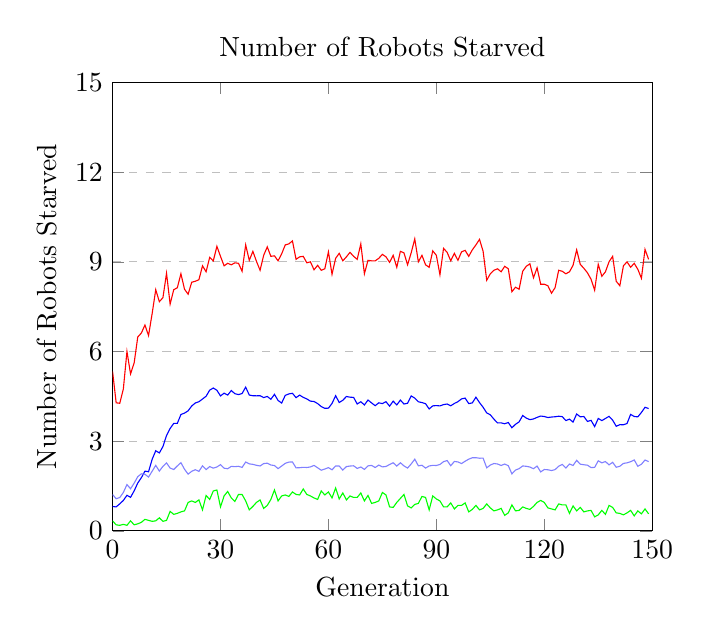
\begin{tikzpicture}
\begin{axis}[
	title={Number of Robots Starved},
	xlabel={Generation},
	ylabel={Number of Robots Starved},
	xmin=0, xmax=150,
	ymin=0, ymax=15,
	xtick={0.0,30.0,60.0,90.0,120.0,150.0},
	ytick={0.0,3.0,6.0,9.0,12.0,15.0},
	ymajorgrids=true,
	grid style=dashed,
]

\addplot[
	color=red,
	]
	coordinates {
	(0,5.333333333333332)(1,4.283333333333334)(2,4.266666666666667)(3,4.75)(4,5.999999999999999)(5,5.250000000000001)(6,5.616666666666668)(7,6.483333333333334)(8,6.616666666666668)(9,6.883333333333335)(10,6.533333333333334)(11,7.266666666666667)(12,8.066666666666666)(13,7.666666666666667)(14,7.800000000000001)(15,8.616666666666667)(16,7.583333333333334)(17,8.066666666666668)(18,8.133333333333333)(19,8.6)(20,8.083333333333334)(21,7.916666666666665)(22,8.316666666666666)(23,8.35)(24,8.399999999999999)(25,8.866666666666665)(26,8.666666666666664)(27,9.15)(28,9.033333333333331)(29,9.516666666666664)(30,9.183333333333332)(31,8.866666666666667)(32,8.950000000000001)(33,8.9)(34,8.966666666666669)(35,8.95)(36,8.683333333333332)(37,9.566666666666666)(38,9.05)(39,9.35)(40,9.016666666666666)(41,8.716666666666667)(42,9.216666666666669)(43,9.5)(44,9.183333333333335)(45,9.2)(46,9.033333333333335)(47,9.266666666666667)(48,9.566666666666666)(49,9.600000000000001)(50,9.700000000000001)(51,9.083333333333332)(52,9.166666666666668)(53,9.183333333333334)(54,8.966666666666667)(55,9.0)(56,8.733333333333333)(57,8.883333333333331)(58,8.716666666666667)(59,8.766666666666666)(60,9.333333333333332)(61,8.583333333333334)(62,9.116666666666667)(63,9.283333333333331)(64,9.033333333333333)(65,9.166666666666666)(66,9.316666666666665)(67,9.18333333333333)(68,9.083333333333336)(69,9.6)(70,8.6)(71,9.049999999999999)(72,9.033333333333335)(73,9.033333333333333)(74,9.116666666666665)(75,9.25)(76,9.166666666666664)(77,8.983333333333333)(78,9.216666666666667)(79,8.816666666666666)(80,9.350000000000001)(81,9.299999999999997)(82,8.899999999999997)(83,9.299999999999999)(84,9.766666666666666)(85,8.999999999999998)(86,9.216666666666667)(87,8.899999999999999)(88,8.816666666666665)(89,9.366666666666667)(90,9.216666666666665)(91,8.566666666666666)(92,9.45)(93,9.316666666666665)(94,9.033333333333333)(95,9.283333333333333)(96,9.05)(97,9.333333333333336)(98,9.383333333333335)(99,9.183333333333334)(100,9.4)(101,9.566666666666668)(102,9.750000000000002)(103,9.35)(104,8.383333333333333)(105,8.600000000000001)(106,8.716666666666665)(107,8.766666666666667)(108,8.666666666666666)(109,8.850000000000003)(110,8.766666666666666)(111,8.0)(112,8.149999999999999)(113,8.083333333333334)(114,8.683333333333334)(115,8.849999999999998)(116,8.933333333333334)(117,8.466666666666667)(118,8.8)(119,8.25)(120,8.25)(121,8.200000000000001)(122,7.95)(123,8.133333333333333)(124,8.716666666666667)(125,8.683333333333332)(126,8.6)(127,8.666666666666666)(128,8.883333333333333)(129,9.4)(130,8.916666666666668)(131,8.783333333333335)(132,8.633333333333335)(133,8.416666666666666)(134,8.049999999999999)(135,8.916666666666666)(136,8.516666666666666)(137,8.666666666666666)(138,9.0)(139,9.183333333333335)(140,8.35)(141,8.200000000000001)(142,8.866666666666667)(143,9.0)(144,8.816666666666665)(145,8.95)(146,8.749999999999998)(147,8.449999999999998)(148,9.416666666666666)(149,9.083333333333334)
	};
\addplot[
	color=blue,
	]
	coordinates {
	(0,0.8138888888888889)(1,0.8)(2,0.9034722222222221)(3,1.015972222222222)(4,1.1881944444444448)(5,1.1201388888888888)(6,1.3361111111111112)(7,1.6)(8,1.775694444444444)(9,1.997222222222222)(10,1.976388888888889)(11,2.3916666666666666)(12,2.678472222222223)(13,2.604861111111111)(14,2.8194444444444446)(15,3.1895833333333337)(16,3.4243055555555553)(17,3.594444444444444)(18,3.5944444444444454)(19,3.8916666666666666)(20,3.9381944444444446)(21,4.013888888888888)(22,4.176388888888888)(23,4.2770833333333345)(24,4.319444444444445)(25,4.409722222222221)(26,4.502083333333332)(27,4.707638888888889)(28,4.777777777777778)(29,4.702083333333333)(30,4.511805555555555)(31,4.605555555555555)(32,4.541666666666666)(33,4.693055555555556)(34,4.5881944444444445)(35,4.557638888888889)(36,4.593055555555555)(37,4.806944444444445)(38,4.542361111111111)(39,4.519444444444444)(40,4.5166666666666675)(41,4.520138888888889)(42,4.456944444444445)(43,4.496527777777778)(44,4.399305555555556)(45,4.566666666666667)(46,4.361805555555556)(47,4.275)(48,4.531249999999999)(49,4.580555555555556)(50,4.6006944444444455)(51,4.455555555555557)(52,4.540277777777777)(53,4.464583333333333)(54,4.4131944444444455)(55,4.338194444444444)(56,4.326388888888888)(57,4.256944444444444)(58,4.156944444444444)(59,4.098611111111111)(60,4.103472222222223)(61,4.260416666666667)(62,4.520833333333333)(63,4.293055555555556)(64,4.368055555555555)(65,4.493055555555555)(66,4.471527777777778)(67,4.4631944444444445)(68,4.2437499999999995)(69,4.3187500000000005)(70,4.211111111111111)(71,4.376388888888888)(72,4.278472222222223)(73,4.186805555555556)(74,4.282638888888889)(75,4.256944444444445)(76,4.319444444444445)(77,4.1715277777777775)(78,4.3381944444444445)(79,4.211805555555555)(80,4.374305555555556)(81,4.241666666666666)(82,4.268055555555555)(83,4.5125)(84,4.440277777777777)(85,4.316666666666666)(86,4.291666666666667)(87,4.252777777777778)(88,4.077083333333334)(89,4.1805555555555545)(90,4.190277777777777)(91,4.179166666666667)(92,4.222222222222222)(93,4.243055555555555)(94,4.181944444444444)(95,4.261111111111111)(96,4.320833333333333)(97,4.41388888888889)(98,4.440972222222222)(99,4.25625)(100,4.279861111111111)(101,4.470833333333335)(102,4.289583333333332)(103,4.133333333333334)(104,3.9444444444444455)(105,3.8812500000000005)(106,3.736805555555555)(107,3.6090277777777775)(108,3.6118055555555557)(109,3.5819444444444444)(110,3.622916666666667)(111,3.447222222222222)(112,3.563888888888889)(113,3.6444444444444453)(114,3.8576388888888884)(115,3.771527777777778)(116,3.7187499999999996)(117,3.743055555555556)(118,3.7951388888888893)(119,3.8395833333333336)(120,3.8243055555555556)(121,3.790277777777778)(122,3.806944444444444)(123,3.815972222222222)(124,3.834027777777777)(125,3.820138888888889)(126,3.688194444444444)(127,3.7368055555555557)(128,3.6375)(129,3.908333333333334)(130,3.814583333333333)(131,3.824305555555555)(132,3.6604166666666664)(133,3.6958333333333333)(134,3.4868055555555553)(135,3.759722222222221)(136,3.6875)(137,3.7583333333333333)(138,3.830555555555555)(139,3.702777777777778)(140,3.4972222222222227)(141,3.551388888888889)(142,3.547916666666666)(143,3.590277777777778)(144,3.89513888888889)(145,3.825)(146,3.8124999999999996)(147,3.9604166666666667)(148,4.131944444444445)(149,4.090972222222222)
	};
\addplot[
	color=green,
	]
	coordinates {
	(0,0.3333333333333333)(1,0.19999999999999998)(2,0.18333333333333332)(3,0.21666666666666665)(4,0.18333333333333332)(5,0.3333333333333333)(6,0.19999999999999998)(7,0.2333333333333333)(8,0.2833333333333333)(9,0.3833333333333333)(10,0.35)(11,0.31666666666666665)(12,0.3333333333333333)(13,0.4333333333333333)(14,0.31666666666666665)(15,0.35)(16,0.65)(17,0.5500000000000002)(18,0.5833333333333334)(19,0.6333333333333335)(20,0.6666666666666666)(21,0.95)(22,1.0)(23,0.9500000000000002)(24,1.0333333333333334)(25,0.7)(26,1.1833333333333333)(27,1.05)(28,1.3333333333333335)(29,1.3666666666666665)(30,0.7999999999999999)(31,1.1666666666666667)(32,1.3166666666666669)(33,1.1)(34,0.9833333333333335)(35,1.2166666666666666)(36,1.2166666666666666)(37,0.9999999999999999)(38,0.7)(39,0.8166666666666667)(40,0.9500000000000001)(41,1.0333333333333334)(42,0.75)(43,0.8500000000000001)(44,1.05)(45,1.3666666666666667)(46,1.0)(47,1.1666666666666667)(48,1.2)(49,1.1500000000000001)(50,1.3)(51,1.2166666666666666)(52,1.2)(53,1.4000000000000001)(54,1.216666666666667)(55,1.1666666666666667)(56,1.0999999999999999)(57,1.05)(58,1.3333333333333333)(59,1.2000000000000002)(60,1.3)(61,1.1)(62,1.4333333333333333)(63,1.0666666666666667)(64,1.2666666666666668)(65,1.0333333333333334)(66,1.1666666666666665)(67,1.1166666666666667)(68,1.1166666666666667)(69,1.2666666666666666)(70,1.0)(71,1.1833333333333333)(72,0.9166666666666667)(73,0.9500000000000001)(74,1.0000000000000002)(75,1.2833333333333334)(76,1.2000000000000002)(77,0.8)(78,0.7833333333333334)(79,0.9500000000000001)(80,1.0833333333333335)(81,1.2166666666666668)(82,0.8333333333333334)(83,0.7666666666666667)(84,0.8833333333333334)(85,0.9166666666666667)(86,1.1500000000000001)(87,1.1166666666666667)(88,0.7000000000000002)(89,1.1666666666666667)(90,1.0666666666666667)(91,1.0)(92,0.7999999999999999)(93,0.8)(94,0.9333333333333335)(95,0.7333333333333334)(96,0.85)(97,0.8500000000000001)(98,0.9333333333333333)(99,0.6333333333333333)(100,0.7166666666666667)(101,0.85)(102,0.7000000000000001)(103,0.75)(104,0.9)(105,0.7666666666666668)(106,0.6666666666666666)(107,0.7)(108,0.7500000000000001)(109,0.5166666666666666)(110,0.6)(111,0.8666666666666666)(112,0.6666666666666666)(113,0.6833333333333333)(114,0.7999999999999999)(115,0.75)(116,0.7166666666666667)(117,0.8166666666666667)(118,0.95)(119,1.0166666666666668)(120,0.9500000000000001)(121,0.7666666666666667)(122,0.7333333333333334)(123,0.7)(124,0.8999999999999999)(125,0.8666666666666667)(126,0.8666666666666667)(127,0.5833333333333333)(128,0.8333333333333335)(129,0.6666666666666666)(130,0.7833333333333334)(131,0.6333333333333333)(132,0.6666666666666666)(133,0.6833333333333333)(134,0.4666666666666667)(135,0.5333333333333333)(136,0.6833333333333333)(137,0.55)(138,0.8500000000000001)(139,0.7833333333333334)(140,0.6)(141,0.5833333333333334)(142,0.5333333333333333)(143,0.6)(144,0.6833333333333332)(145,0.5)(146,0.6666666666666666)(147,0.5666666666666667)(148,0.7333333333333334)(149,0.5666666666666667)
	};
\addplot[
	color=blue!50,
	]
	coordinates {
	(0,1.214375069310571)(1,1.0736034201974722)(2,1.1122919690270947)(3,1.284239541788178)(4,1.5472133213149948)(5,1.4063704647757718)(6,1.595249825892092)(7,1.8106980683347846)(8,1.9073758922338686)(9,1.8920725363298703)(10,1.7979819778741817)(11,1.993063995052394)(12,2.1900490349949937)(13,1.997953683506368)(14,2.1570283143747253)(15,2.270781537471653)(16,2.09900280022863)(17,2.050824070791015)(18,2.1701282459035207)(19,2.2809984754075376)(20,2.0595377416692298)(21,1.897376426996611)(22,1.990557753842954)(23,2.045096354467822)(24,1.9875869443370422)(25,2.1743077278359886)(26,2.0489326672423402)(27,2.149235780820617)(28,2.0966181150127405)(29,2.1362847042094124)(30,2.214237252692144)(31,2.095235094592308)(32,2.0770042802506223)(33,2.1572454281726556)(34,2.146105955062889)(35,2.1585917524616742)(36,2.121858633469183)(37,2.3008321187613543)(38,2.2392625472858145)(39,2.2237682107611327)(40,2.19150407963177)(41,2.169866862451167)(42,2.2491566338953732)(43,2.263487544900315)(44,2.201351850862929)(45,2.184092307085963)(46,2.0807880011486595)(47,2.1678577855549834)(48,2.25756121075359)(49,2.299358950791794)(50,2.304085885989994)(51,2.106357137488005)(52,2.111603560374565)(53,2.1238780764300973)(54,2.118466400731342)(55,2.1374295738708824)(56,2.1888420247076583)(57,2.1097289769083654)(58,2.0280191781860766)(59,2.0663912281316543)(60,2.1143189743057484)(61,2.0413101590592237)(62,2.168269920112139)(63,2.167415421205554)(64,2.029875324301901)(65,2.1496912992846267)(66,2.1667809497194725)(67,2.17549000098798)(68,2.0873359904303017)(69,2.135191489053526)(70,2.0553022383605293)(71,2.1730813283775725)(72,2.188265826477382)(73,2.117746501065295)(74,2.197704767968628)(75,2.1385237849988754)(76,2.152753145298509)(77,2.218225055619464)(78,2.277610393377392)(79,2.164748068357655)(80,2.2772838928767762)(81,2.171792632866222)(82,2.0990345789364437)(83,2.237182429278632)(84,2.3974039639880558)(85,2.1731689478379392)(86,2.1929238198203422)(87,2.0984412939014256)(88,2.1691330940840197)(89,2.189301806463639)(90,2.185175503978832)(91,2.219644178006352)(92,2.314574403939954)(93,2.35107666805518)(94,2.177937679729833)(95,2.319810208642119)(96,2.3052587578082493)(97,2.2494773308081726)(98,2.327843967860841)(99,2.396840941537158)(100,2.4441266643170074)(101,2.4452546390129695)(102,2.4290744559551967)(103,2.431015269177646)(104,2.1069389549127395)(105,2.200637796158195)(106,2.2517795682987467)(107,2.2356813237959843)(108,2.186195747645317)(109,2.233395993546768)(110,2.17806269194566)(111,1.9061043289583444)(112,2.0321180532823693)(113,2.0807888253448215)(114,2.170403205191987)(115,2.1585027393100575)(116,2.1338739525530164)(117,2.077907920927997)(118,2.1660925242096867)(119,1.970266833812838)(120,2.0509335275120817)(121,2.0420725008450153)(122,2.0169917909545827)(123,2.047327724681277)(124,2.1601131418731496)(125,2.2211687091059473)(126,2.099370205503855)(127,2.235580374948403)(128,2.186101118465192)(129,2.3577843501870843)(130,2.229477404067396)(131,2.210563250139664)(132,2.1947962377989447)(133,2.1155365276937492)(134,2.122229787986447)(135,2.342084637618263)(136,2.2752050494381524)(137,2.3162314621512325)(138,2.2072623559321802)(139,2.2916809113278487)(140,2.126281136723843)(141,2.1603478092283983)(142,2.2549015881110295)(143,2.273783043547513)(144,2.3119772298459353)(145,2.371777003599441)(146,2.159347321347553)(147,2.2276022587261144)(148,2.368394313099643)(149,2.3161921596702224)
	};
\end{axis}
\end{tikzpicture}
}
		\caption{Some sample caption}
	\end{subfigure}%
	\begin{subfigure}[b]{0.7\textwidth}
		\centering
		\resizebox{0.9\linewidth}{!}{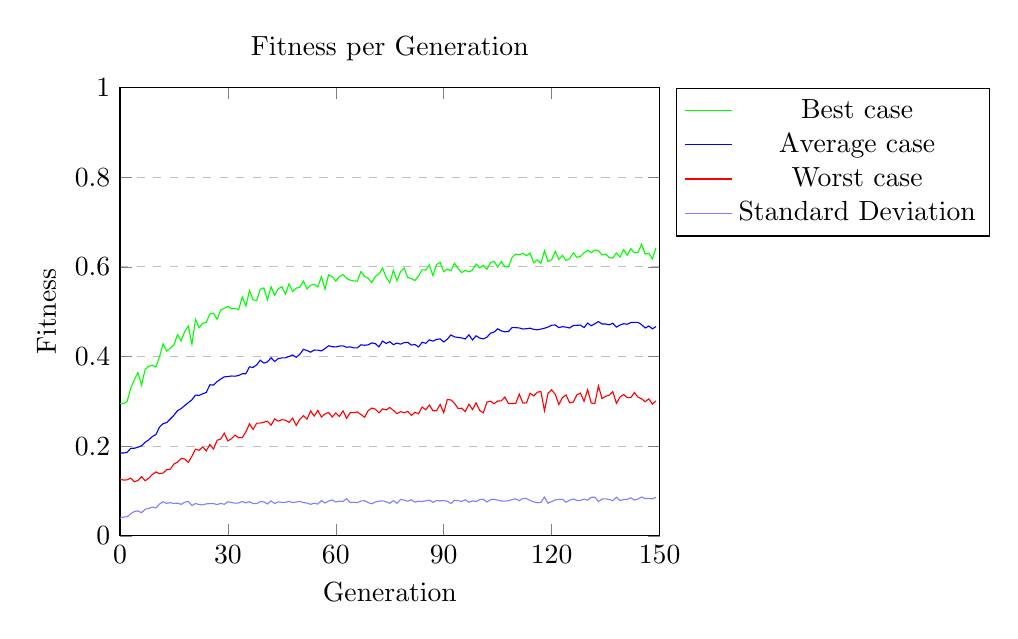
\begin{tikzpicture}
\begin{axis}[
	title={Fitness per Generation},
	xlabel={Generation},
	ylabel={Fitness},
	xmin=0, xmax=150,
	ymin=0, ymax=1,
	xtick={0.0,30.0,60.0,90.0,120.0,150.0},
	ytick={0.0,0.2,0.4,0.6000000000000001,0.8,1.0},
	legend pos=outer north east,
	ymajorgrids=true,
	grid style=dashed,
]

\addplot[
	color=green,
	]
	coordinates {
	(0,0.2957235)(1,0.29496066666666676)(2,0.29999025)(3,0.3294585)(4,0.3483075833333333)(5,0.3640961666666666)(6,0.33639766666666665)(7,0.37115925000000005)(8,0.37833283333333334)(9,0.3806003333333333)(10,0.3766358333333334)(11,0.39966383333333333)(12,0.4283990000000001)(13,0.41237225)(14,0.41898066666666667)(15,0.42601858333333337)(16,0.44872733333333326)(17,0.43491541666666667)(18,0.4554935)(19,0.467992)(20,0.42726675)(21,0.4831623333333333)(22,0.4646263333333333)(23,0.4740057499999999)(24,0.47653974999999993)(25,0.4949525833333333)(26,0.4968383333333335)(27,0.4831203333333333)(28,0.5035778333333334)(29,0.5077855)(30,0.5116675)(31,0.5064385)(32,0.50725175)(33,0.5048266666666666)(34,0.5330411666666666)(35,0.5126704166666666)(36,0.54733225)(37,0.5265828333333332)(38,0.5246354166666667)(39,0.54985625)(40,0.5530321666666667)(41,0.5265258333333332)(42,0.5557229166666667)(43,0.5367625833333333)(44,0.5512059999999999)(45,0.5559528333333333)(46,0.53956925)(47,0.5621102499999999)(48,0.5451053333333333)(49,0.55253075)(50,0.5546189166666666)(51,0.56826325)(52,0.5507675833333333)(53,0.5592520833333333)(54,0.5609246666666668)(55,0.5552625)(56,0.5781009166666669)(57,0.5503075000000001)(58,0.5823069166666667)(59,0.5783853333333334)(60,0.5682005)(61,0.5782875833333333)(62,0.5829162499999999)(63,0.5744158333333333)(64,0.5704008333333332)(65,0.5687644166666666)(66,0.5682826666666667)(67,0.5897009166666667)(68,0.5786665833333333)(69,0.5742185833333333)(70,0.5650825)(71,0.57881575)(72,0.5843008333333333)(73,0.5972431666666668)(74,0.5767831666666666)(75,0.56480025)(76,0.5926253333333336)(77,0.5688773333333333)(78,0.5896958333333333)(79,0.5974019166666666)(80,0.5764375833333333)(81,0.5735556666666666)(82,0.5696878333333335)(83,0.5796616666666665)(84,0.5934859166666667)(85,0.5929356666666666)(86,0.6041665)(87,0.5805803333333333)(88,0.6049383333333334)(89,0.6101501666666668)(90,0.5891455833333333)(91,0.5950436666666667)(92,0.5915253333333335)(93,0.6080413333333332)(94,0.5960230833333334)(95,0.5873436666666666)(96,0.59231225)(97,0.5889880833333334)(98,0.5929996666666667)(99,0.6064123333333333)(100,0.5981699166666667)(101,0.6032054166666667)(102,0.5944826666666667)(103,0.6092784166666667)(104,0.6122195833333333)(105,0.5996504166666666)(106,0.6119505)(107,0.6002088333333333)(108,0.6003550000000001)(109,0.6210048333333333)(110,0.6285391666666669)(111,0.6268122500000002)(112,0.6302600833333334)(113,0.6250974166666667)(114,0.6308829166666667)(115,0.6091084999999999)(116,0.6156460833333334)(117,0.60799725)(118,0.6358656666666667)(119,0.61208375)(120,0.6159948333333334)(121,0.6347230833333334)(122,0.6167196666666666)(123,0.6257711666666665)(124,0.61439825)(125,0.6180035)(126,0.6313494166666667)(127,0.6215813333333333)(128,0.6231217500000001)(129,0.6313521666666667)(130,0.63699075)(131,0.6317695833333333)(132,0.6377607499999999)(133,0.6362829999999999)(134,0.6265881666666666)(135,0.6287284999999999)(136,0.6208665833333333)(137,0.6197110833333332)(138,0.6309479166666667)(139,0.6220475000000001)(140,0.6385080833333332)(141,0.6257754166666667)(142,0.6409095833333334)(143,0.6314705)(144,0.6321538333333334)(145,0.6508091666666668)(146,0.6284318333333334)(147,0.6306168333333333)(148,0.6180559166666666)(149,0.6427430833333334)
	};
	\addlegendentry{Best case}
\addplot[
	color=blue,
	]
	coordinates {
	(0,0.18497803819444442)(1,0.18483698611111113)(2,0.18635468055555554)(3,0.19531263194444448)(4,0.19545605208333333)(5,0.19774555902777777)(6,0.20106962152777774)(7,0.20879207291666665)(8,0.2141435034722223)(9,0.22158321527777777)(10,0.22599069097222219)(11,0.2427119861111111)(12,0.2503866701388889)(13,0.2527525798611111)(14,0.26084429861111114)(15,0.2689861944444445)(16,0.27929395833333337)(17,0.2838712152777778)(18,0.2906418229166666)(19,0.29709476388888884)(20,0.30358085416666664)(21,0.31402249305555563)(22,0.31334752430555557)(23,0.3169582048611112)(24,0.3199585104166667)(25,0.3371130659722222)(26,0.3363696631944445)(27,0.34425006597222224)(28,0.3497767395833333)(29,0.3547384930555556)(30,0.3554077430555555)(31,0.3566488958333333)(32,0.3561557222222222)(33,0.35787572916666666)(34,0.3616385902777779)(35,0.3617647222222223)(36,0.3770551597222222)(37,0.37582047916666667)(38,0.3814128819444444)(39,0.39181162847222223)(40,0.3855090416666666)(41,0.3882156423611111)(42,0.3971997222222223)(43,0.38908529513888895)(44,0.39546750347222215)(45,0.39706302777777774)(46,0.39700321875000005)(47,0.40037732638888895)(48,0.40347893749999997)(49,0.3984317013888889)(50,0.4049912013888889)(51,0.41615034375)(52,0.4133683715277778)(53,0.40977615972222226)(54,0.4145734791666666)(55,0.41434615625000004)(56,0.41261092361111107)(57,0.41793836458333333)(58,0.4241021979166666)(59,0.4220220034722222)(60,0.42158328472222223)(61,0.42340279861111113)(62,0.42396321875000004)(63,0.4207747604166667)(64,0.42162345833333337)(65,0.4194042604166667)(66,0.41930434375)(67,0.4262195)(68,0.4251634618055556)(69,0.4261131840277777)(70,0.43055798263888884)(71,0.4287785381944445)(72,0.4216186979166667)(73,0.43460982986111113)(74,0.4290612256944445)(75,0.43333210416666657)(76,0.42637912152777774)(77,0.4301452083333334)(78,0.42766290625)(79,0.43112295138888884)(80,0.4317012916666667)(81,0.42555036458333334)(82,0.4268411076388889)(83,0.42137639236111113)(84,0.4318554236111112)(85,0.42955075000000004)(86,0.43732140625)(87,0.43440073611111113)(88,0.43813386805555554)(89,0.43948687499999994)(90,0.4324347777777777)(91,0.43878389236111104)(92,0.4483032569444444)(93,0.44379063888888887)(94,0.44270752083333337)(95,0.4415039201388888)(96,0.4392663854166667)(97,0.4484658645833334)(98,0.4371128333333334)(99,0.44641384375)(100,0.44126367361111113)(101,0.43937157986111103)(102,0.44306244791666666)(103,0.4521707638888888)(104,0.45463993750000004)(105,0.4618523784722222)(106,0.45720568750000007)(107,0.45524034375000005)(108,0.45578383680555556)(109,0.46473991666666675)(110,0.4644812430555556)(111,0.4638426736111111)(112,0.46141506944444444)(113,0.4621067673611111)(114,0.4632951284722223)(115,0.46073170138888886)(116,0.459579045138889)(117,0.4612494618055555)(118,0.4632245104166667)(119,0.46599322222222217)(120,0.46988265277777774)(121,0.4704529687499999)(122,0.46454634027777786)(123,0.46669313194444445)(124,0.4656560590277778)(125,0.4637363298611112)(126,0.46926321180555564)(127,0.4697050381944444)(128,0.47012597916666665)(129,0.46467917708333345)(130,0.47475089583333335)(131,0.46868044444444434)(132,0.47308472916666666)(133,0.4780976111111111)(134,0.4724788194444445)(135,0.47273138541666676)(136,0.4708417638888889)(137,0.4742129513888889)(138,0.46566382638888887)(139,0.4704004027777777)(140,0.47329688194444447)(141,0.4720240937500001)(142,0.4758357743055555)(143,0.4762649166666667)(144,0.4763519583333334)(145,0.47099225)(146,0.46369127777777785)(147,0.4681310069444444)(148,0.46179327777777784)(149,0.46690240624999996)
	};
	\addlegendentry{Average case}
\addplot[
	color=red,
	]
	coordinates {
	(0,0.12599725)(1,0.12458066666666667)(2,0.12495133333333334)(3,0.12889216666666667)(4,0.12071025)(5,0.12359991666666668)(6,0.1320801666666667)(7,0.12295850000000003)(8,0.1287360833333333)(9,0.1368583333333333)(10,0.14276416666666664)(11,0.13859183333333333)(12,0.14028674999999996)(13,0.14751666666666666)(14,0.14881300000000003)(15,0.16026516666666665)(16,0.16458408333333333)(17,0.17270966666666665)(18,0.1714839166666667)(19,0.16383041666666667)(20,0.17754583333333337)(21,0.19339441666666665)(22,0.19097866666666666)(23,0.19816950000000003)(24,0.1896810833333334)(25,0.20395933333333335)(26,0.19367624999999997)(27,0.21320975)(28,0.21606299999999998)(29,0.22903658333333332)(30,0.21171933333333331)(31,0.21685833333333335)(32,0.2248549166666667)(33,0.2187573333333333)(34,0.21935449999999998)(35,0.23163791666666667)(36,0.25008258333333333)(37,0.23741750000000003)(38,0.25133825)(39,0.2516130833333333)(40,0.25353699999999996)(41,0.2557184166666667)(42,0.2469069166666667)(43,0.26090125)(44,0.25613891666666666)(45,0.25934008333333336)(46,0.2579246666666667)(47,0.25338483333333334)(48,0.2625172499999999)(49,0.24628366666666662)(50,0.2601339166666667)(51,0.2682243333333334)(52,0.2604035)(53,0.27867725)(54,0.2671275833333333)(55,0.27991375000000007)(56,0.26516366666666663)(57,0.27203808333333335)(58,0.275219)(59,0.2651574166666667)(60,0.2741805)(61,0.2665225)(62,0.2790255833333333)(63,0.2623101666666667)(64,0.2747138333333333)(65,0.27515808333333336)(66,0.27629125000000004)(67,0.27052908333333336)(68,0.2645102500000001)(69,0.2794308333333333)(70,0.2851645833333333)(71,0.28264716666666667)(72,0.2743250833333334)(73,0.2833968333333333)(74,0.280937)(75,0.2864446666666667)(76,0.27986683333333334)(77,0.27269224999999997)(78,0.27716366666666664)(79,0.27481441666666667)(80,0.2776808333333334)(81,0.26879033333333335)(82,0.27549108333333333)(83,0.27254900000000004)(84,0.2873580000000001)(85,0.28152141666666664)(86,0.29198133333333337)(87,0.27913525)(88,0.27926091666666664)(89,0.29333725)(90,0.2748808333333334)(91,0.3044426666666667)(92,0.30318791666666667)(93,0.29564841666666664)(94,0.28425458333333337)(95,0.2846751666666667)(96,0.27727883333333336)(97,0.2937841666666666)(98,0.28162008333333327)(99,0.29692716666666663)(100,0.27959100000000003)(101,0.27448975)(102,0.2984453333333333)(103,0.3004046666666666)(104,0.29479041666666667)(105,0.3009759166666667)(106,0.3010049166666666)(107,0.3096170833333333)(108,0.29491433333333333)(109,0.29529808333333335)(110,0.2952863333333334)(111,0.31620224999999996)(112,0.2961041666666667)(113,0.2968300833333334)(114,0.3182321666666667)(115,0.31238241666666666)(116,0.32034125)(117,0.3221835833333333)(118,0.2790804166666667)(119,0.31833666666666666)(120,0.3258068333333333)(121,0.31556125)(122,0.29302041666666667)(123,0.30869033333333334)(124,0.31432699999999997)(125,0.2968261666666667)(126,0.29847741666666666)(127,0.3146143333333334)(128,0.31861766666666663)(129,0.30009691666666666)(130,0.32610808333333335)(131,0.2962863333333333)(132,0.29518075000000005)(133,0.33464733333333335)(134,0.3062048333333333)(135,0.31145900000000004)(136,0.3138266666666666)(137,0.32164875)(138,0.29582325)(139,0.3096729166666667)(140,0.3153906666666667)(141,0.3084745)(142,0.3083290000000001)(143,0.3200254166666667)(144,0.30941066666666667)(145,0.30600475000000005)(146,0.2992341666666666)(147,0.30567275)(148,0.293882)(149,0.30102816666666665)
	};
	\addlegendentry{Worst case}
\addplot[
	color=blue!50,
	]
	coordinates {
	(0,0.03961706201573329)(1,0.04201099087911795)(2,0.04269846538827712)(3,0.049292622586127106)(4,0.0544488732561116)(5,0.055803199610043375)(6,0.05183277680029281)(7,0.059441305387755355)(8,0.06136196130918438)(9,0.06444715396220287)(10,0.06234407303261757)(11,0.07095207326281876)(12,0.07617758228423555)(13,0.07255351663612704)(14,0.07411588490079284)(15,0.07228404165625464)(16,0.07297291698547226)(17,0.07034410357650496)(18,0.07516913313643139)(19,0.07694383399207508)(20,0.06767964275905379)(21,0.07227594062303995)(22,0.06987026527722626)(23,0.06913467628468016)(24,0.07143863587776056)(25,0.07202427534578451)(26,0.07215184449860924)(27,0.06984657570562729)(28,0.0725557778186721)(29,0.07053167234854212)(30,0.07611839138414295)(31,0.07454096225936789)(32,0.07292862156100414)(33,0.07352363872765692)(34,0.07670916558591845)(35,0.07349800296429065)(36,0.0764664050435616)(37,0.07211421937295417)(38,0.07187799332961452)(39,0.07642339816019675)(40,0.0759313734188884)(41,0.0711400052431247)(42,0.07809251673253835)(43,0.07224166792543674)(44,0.07596946740938101)(45,0.0747323502086181)(46,0.0747282157291644)(47,0.07713800055485208)(48,0.07429828865487584)(49,0.07553270038731084)(50,0.07683645106697064)(51,0.07428081088728507)(52,0.07318173692652094)(53,0.07041444385391755)(54,0.07286083878784072)(55,0.07090162744332835)(56,0.07873776159115752)(57,0.07328952325738887)(58,0.07763072985245775)(59,0.08030805501071896)(60,0.07538145545949411)(61,0.07749472134709808)(62,0.07688587112767088)(63,0.08305050148693693)(64,0.07435540115461732)(65,0.07499821117496873)(66,0.07426011646576018)(67,0.07779283598069092)(68,0.0785138365680607)(69,0.0743218184809134)(70,0.07151279062232406)(71,0.07573044201252027)(72,0.07749555036975672)(73,0.07815217779917483)(74,0.0760235512700237)(75,0.07269821517614847)(76,0.0789978721230877)(77,0.07261649071107278)(78,0.08131245858630246)(79,0.07992528123628917)(80,0.07730461577262372)(81,0.08056395919413234)(82,0.07528480859449542)(83,0.07720093600065144)(84,0.07657778618846815)(85,0.07813853849921563)(86,0.07960564719079789)(87,0.07494780171647117)(88,0.07881434763220166)(89,0.07827967474907364)(90,0.07864735944155217)(91,0.07728567420036209)(92,0.0722205589102382)(93,0.07945874323006331)(94,0.07857544828918114)(95,0.07716044046956277)(96,0.08054149292234002)(97,0.07506074844796665)(98,0.07804659953203878)(99,0.07656938289002567)(100,0.0807377712934465)(101,0.08176589184250577)(102,0.07550451854176292)(103,0.08092260597088492)(104,0.08159228633070939)(105,0.07982851784478243)(106,0.07792300625916937)(107,0.07741457459695728)(108,0.07862615550506957)(109,0.0809178926055889)(110,0.08249149770973298)(111,0.07835389072805483)(112,0.08356070406569308)(113,0.08342691761663125)(114,0.07894345738621991)(115,0.07599973339461844)(116,0.07399442762376142)(117,0.07444727324427952)(118,0.08673157512181062)(119,0.07260417273916024)(120,0.07670434720870456)(121,0.08034983989930479)(122,0.08136933022110146)(123,0.08156617014757828)(124,0.07501207002567666)(125,0.07973478944580414)(126,0.08237587798145517)(127,0.07893593478014362)(128,0.07922946045756472)(129,0.0820561905826228)(130,0.07972148208853677)(131,0.08598759572481587)(132,0.08642907413172747)(133,0.07662824212276954)(134,0.08224009060001856)(135,0.0826223764105586)(136,0.08100118692160077)(137,0.0783828625461216)(138,0.08621816761456191)(139,0.07894109585931916)(140,0.08118491956634606)(141,0.08155508766850118)(142,0.08493341665777995)(143,0.07982649114559821)(144,0.08223859979304267)(145,0.08673659865218858)(146,0.0833590422891152)(147,0.08343225837536715)(148,0.08258089902513811)(149,0.08616170925029497)
	};
	\addlegendentry{Standard Deviation}
\end{axis}
\end{tikzpicture}
}
		\caption{Some sample caption}
	\end{subfigure}%
}
\end{figure}

\newpage
\vspace*{-2.0cm}
\textbf{\Huge LARGE SAMPLE HEADER}
\vspace{1.5cm}
\begin{tikzpicture}[remember picture,overlay]
   \node[anchor=south east,inner sep=20pt] at (current page.south east)
              {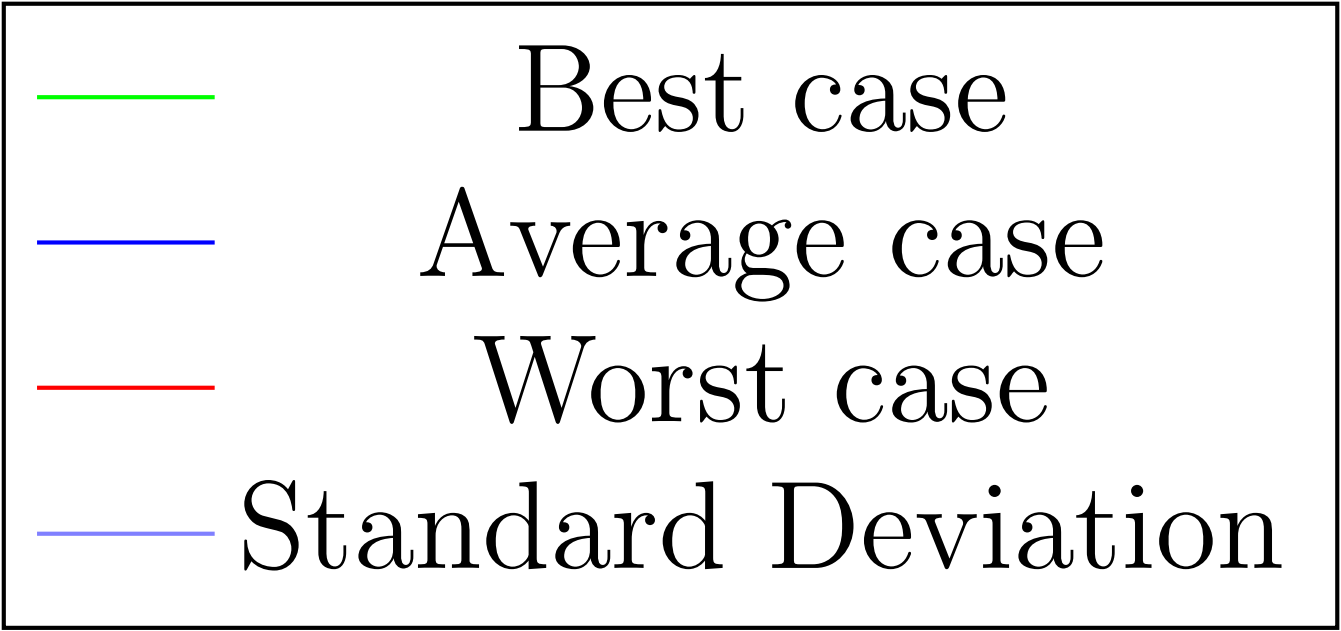
\includegraphics[scale=0.1]{chapters/res/generated_graph_legend.png}};
\end{tikzpicture}

\begin{figure}[H]
\vspace*{-1cm}
	\makebox[\linewidth][c]{%
	\begin{subfigure}[b]{0.7\textwidth}
		\centering
		\resizebox{0.9\linewidth}{!}{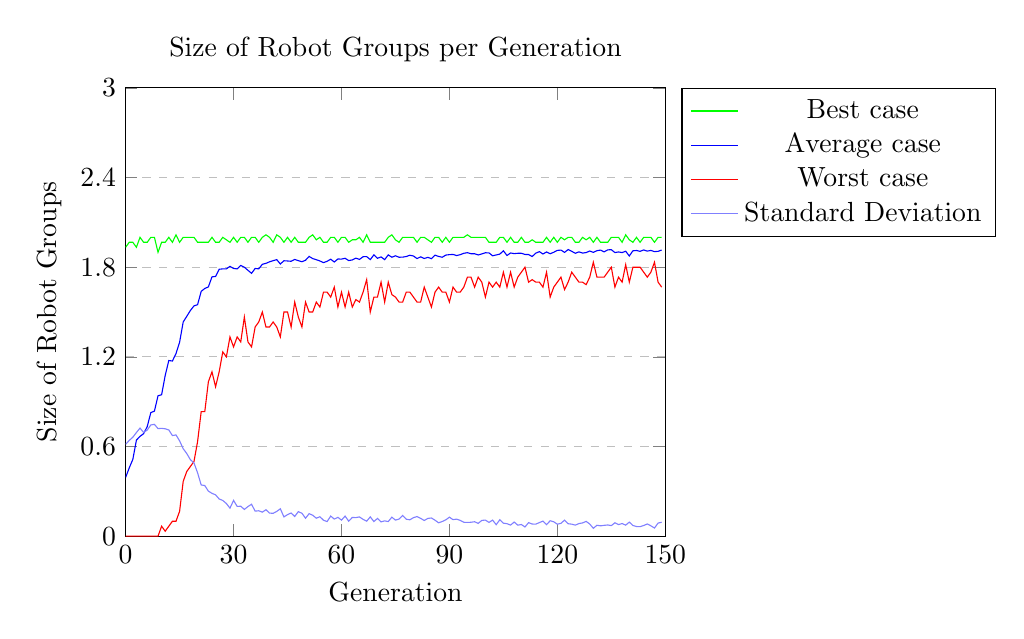
\begin{tikzpicture}
\begin{axis}[
	title={Size of Robot Groups per Generation},
	xlabel={Generation},
	ylabel={Size of Robot Groups},
	xmin=0, xmax=150,
	ymin=0, ymax=3,
	xtick={0.0,30.0,60.0,90.0,120.0,150.0},
	ytick={0.0,0.6,1.2,1.7999999999999998,2.4,3.0},
	legend pos=outer north east,
	ymajorgrids=true,
	grid style=dashed,
]

\addplot[
	color=green,
	]
	coordinates {
	(0,1.9333333333333338)(1,1.9666666666666672)(2,1.9666666666666672)(3,1.9333333333333338)(4,2.0000000000000004)(5,1.9666666666666672)(6,1.9666666666666672)(7,2.0000000000000004)(8,2.0000000000000004)(9,1.9000000000000008)(10,1.9666666666666672)(11,1.9666666666666675)(12,2.0000000000000004)(13,1.9666666666666675)(14,2.016666666666667)(15,1.9666666666666672)(16,2.0000000000000004)(17,2.0000000000000004)(18,2.0000000000000004)(19,2.0000000000000004)(20,1.9666666666666672)(21,1.9666666666666672)(22,1.9666666666666672)(23,1.9666666666666672)(24,2.0000000000000004)(25,1.9666666666666672)(26,1.9666666666666672)(27,2.0000000000000004)(28,1.983333333333334)(29,1.9666666666666672)(30,2.0000000000000004)(31,1.9666666666666672)(32,2.0000000000000004)(33,2.0000000000000004)(34,1.9666666666666672)(35,2.0000000000000004)(36,2.0000000000000004)(37,1.9666666666666672)(38,2.0000000000000004)(39,2.016666666666667)(40,2.0000000000000004)(41,1.9666666666666675)(42,2.0166666666666675)(43,2.0000000000000004)(44,1.9666666666666675)(45,2.0000000000000004)(46,1.9666666666666675)(47,2.0000000000000004)(48,1.9666666666666675)(49,1.9666666666666675)(50,1.9666666666666675)(51,2.0000000000000004)(52,2.0166666666666675)(53,1.983333333333334)(54,2.0000000000000004)(55,1.9666666666666675)(56,1.9666666666666675)(57,2.0000000000000004)(58,2.0000000000000004)(59,1.9666666666666675)(60,2.0000000000000004)(61,2.0000000000000004)(62,1.9666666666666675)(63,1.983333333333334)(64,1.983333333333334)(65,2.0000000000000004)(66,1.9666666666666675)(67,2.016666666666667)(68,1.9666666666666675)(69,1.9666666666666675)(70,1.9666666666666675)(71,1.9666666666666675)(72,1.9666666666666675)(73,2.0000000000000004)(74,2.016666666666667)(75,1.983333333333334)(76,1.9666666666666675)(77,2.0000000000000004)(78,2.0000000000000004)(79,2.0000000000000004)(80,2.0000000000000004)(81,1.9666666666666675)(82,2.0000000000000004)(83,2.0000000000000004)(84,1.983333333333334)(85,1.9666666666666675)(86,2.0000000000000004)(87,2.0000000000000004)(88,1.9666666666666675)(89,2.0000000000000004)(90,1.9666666666666675)(91,2.0000000000000004)(92,2.0000000000000004)(93,2.0000000000000004)(94,2.0000000000000004)(95,2.016666666666667)(96,2.0000000000000004)(97,2.0000000000000004)(98,2.0000000000000004)(99,2.0000000000000004)(100,2.0000000000000004)(101,1.9666666666666675)(102,1.9666666666666675)(103,1.9666666666666675)(104,2.0000000000000004)(105,2.0000000000000004)(106,1.9666666666666675)(107,2.0000000000000004)(108,1.9666666666666675)(109,1.9666666666666675)(110,2.0000000000000004)(111,1.9666666666666675)(112,1.9666666666666675)(113,1.983333333333334)(114,1.9666666666666675)(115,1.9666666666666675)(116,1.9666666666666675)(117,2.0000000000000004)(118,1.9666666666666675)(119,2.0000000000000004)(120,1.9666666666666675)(121,2.0000000000000004)(122,1.983333333333334)(123,2.0000000000000004)(124,2.0000000000000004)(125,1.9666666666666675)(126,1.9666666666666675)(127,2.0000000000000004)(128,1.983333333333334)(129,2.0000000000000004)(130,1.9666666666666675)(131,2.0000000000000004)(132,1.9666666666666675)(133,1.9666666666666675)(134,1.9666666666666675)(135,2.0000000000000004)(136,2.0000000000000004)(137,2.0000000000000004)(138,1.9666666666666675)(139,2.0166666666666675)(140,1.983333333333334)(141,1.9666666666666675)(142,2.0000000000000004)(143,1.9666666666666675)(144,2.0000000000000004)(145,2.0000000000000004)(146,2.0000000000000004)(147,1.9666666666666675)(148,2.0000000000000004)(149,2.0000000000000004)
	};
	\addlegendentry{Best case}
\addplot[
	color=blue,
	]
	coordinates {
	(0,0.39305555555555555)(1,0.45694444444444443)(2,0.5138888888888888)(3,0.6430555555555557)(4,0.6680555555555556)(5,0.6861111111111111)(6,0.7333333333333333)(7,0.8270833333333334)(8,0.8368055555555555)(9,0.9395833333333333)(10,0.9465277777777777)(11,1.0756944444444443)(12,1.1756944444444444)(13,1.1722222222222223)(14,1.222222222222222)(15,1.2979166666666664)(16,1.4333333333333331)(17,1.471527777777778)(18,1.5104166666666665)(19,1.540972222222222)(20,1.5493055555555553)(21,1.6381944444444445)(22,1.6576388888888893)(23,1.6680555555555558)(24,1.735416666666667)(25,1.738194444444445)(26,1.7861111111111116)(27,1.7888888888888892)(28,1.7888888888888892)(29,1.805555555555556)(30,1.791666666666667)(31,1.7888888888888894)(32,1.8118055555555561)(33,1.8000000000000005)(34,1.779166666666667)(35,1.7590277777777783)(36,1.791666666666667)(37,1.7888888888888892)(38,1.8194444444444449)(39,1.825694444444445)(40,1.8361111111111115)(41,1.8437500000000007)(42,1.850694444444445)(43,1.8215277777777785)(44,1.8430555555555563)(45,1.8416666666666672)(46,1.839583333333334)(47,1.8520833333333342)(48,1.8437500000000004)(49,1.836805555555556)(50,1.8465277777777784)(51,1.872222222222223)(52,1.8576388888888897)(53,1.8500000000000008)(54,1.8416666666666675)(55,1.8305555555555564)(56,1.839583333333334)(57,1.8534722222222229)(58,1.8347222222222228)(59,1.8548611111111117)(60,1.8541666666666674)(61,1.859722222222223)(62,1.844444444444445)(63,1.8486111111111119)(64,1.8604166666666673)(65,1.852083333333334)(66,1.8701388888888895)(67,1.870833333333334)(68,1.850694444444445)(69,1.8826388888888894)(70,1.8597222222222227)(71,1.8687500000000006)(72,1.8506944444444453)(73,1.8826388888888896)(74,1.8666666666666674)(75,1.8763888888888896)(76,1.8666666666666674)(77,1.8673611111111117)(78,1.8715277777777783)(79,1.8798611111111119)(80,1.8750000000000004)(81,1.8576388888888895)(82,1.8694444444444451)(83,1.8583333333333338)(84,1.8659722222222226)(85,1.856944444444445)(86,1.880555555555556)(87,1.872222222222223)(88,1.8666666666666674)(89,1.8812500000000005)(90,1.8840277777777783)(91,1.8854166666666672)(92,1.8777777777777784)(93,1.8840277777777785)(94,1.8930555555555564)(95,1.8972222222222228)(96,1.8902777777777784)(97,1.8902777777777786)(98,1.881944444444445)(99,1.8888888888888895)(100,1.8965277777777783)(101,1.895833333333334)(102,1.8763888888888896)(103,1.881944444444445)(104,1.8875000000000006)(105,1.9097222222222228)(106,1.8784722222222228)(107,1.8951388888888894)(108,1.8909722222222227)(109,1.8930555555555562)(110,1.8930555555555562)(111,1.8854166666666674)(112,1.8847222222222229)(113,1.8715277777777786)(114,1.8937500000000005)(115,1.9041666666666675)(116,1.888194444444445)(117,1.9020833333333338)(118,1.8902777777777784)(119,1.9000000000000004)(120,1.9125000000000005)(121,1.9145833333333337)(122,1.8993055555555558)(123,1.918055555555556)(124,1.9062500000000002)(125,1.8930555555555562)(126,1.9027777777777781)(127,1.8944444444444448)(128,1.8979166666666674)(129,1.9083333333333339)(130,1.8993055555555562)(131,1.9104166666666673)(132,1.914583333333334)(133,1.9027777777777781)(134,1.9159722222222229)(135,1.9173611111111117)(136,1.8979166666666674)(137,1.902083333333334)(138,1.8979166666666671)(139,1.9069444444444452)(140,1.8750000000000007)(141,1.9097222222222228)(142,1.9118055555555562)(143,1.9062500000000007)(144,1.9152777777777785)(145,1.9076388888888893)(146,1.9125000000000005)(147,1.9041666666666675)(148,1.9062500000000004)(149,1.914583333333334)
	};
	\addlegendentry{Average case}
\addplot[
	color=red,
	]
	coordinates {
	(0,0.0)(1,0.0)(2,0.0)(3,0.0)(4,0.0)(5,0.0)(6,0.0)(7,0.0)(8,0.0)(9,0.0)(10,0.06666666666666667)(11,0.03333333333333333)(12,0.06666666666666667)(13,0.1)(14,0.1)(15,0.16666666666666666)(16,0.3666666666666667)(17,0.43333333333333335)(18,0.4666666666666667)(19,0.5)(20,0.6333333333333333)(21,0.8333333333333333)(22,0.8333333333333333)(23,1.0333333333333332)(24,1.1)(25,0.9999999999999999)(26,1.0999999999999999)(27,1.2333333333333334)(28,1.2)(29,1.3333333333333333)(30,1.2666666666666666)(31,1.3333333333333333)(32,1.3000000000000003)(33,1.4666666666666668)(34,1.3)(35,1.2666666666666666)(36,1.4000000000000001)(37,1.4333333333333336)(38,1.5000000000000002)(39,1.4000000000000001)(40,1.4000000000000001)(41,1.4333333333333333)(42,1.4)(43,1.3333333333333333)(44,1.5000000000000002)(45,1.5000000000000002)(46,1.4)(47,1.5666666666666669)(48,1.4666666666666668)(49,1.4000000000000001)(50,1.5666666666666669)(51,1.5000000000000002)(52,1.5000000000000002)(53,1.5666666666666669)(54,1.5333333333333337)(55,1.6333333333333337)(56,1.6333333333333337)(57,1.6000000000000003)(58,1.666666666666667)(59,1.5333333333333337)(60,1.6333333333333337)(61,1.5333333333333334)(62,1.6333333333333337)(63,1.5333333333333334)(64,1.5833333333333337)(65,1.5666666666666669)(66,1.6333333333333337)(67,1.7166666666666672)(68,1.5000000000000002)(69,1.6000000000000003)(70,1.6000000000000003)(71,1.7000000000000004)(72,1.5666666666666669)(73,1.7000000000000004)(74,1.616666666666667)(75,1.6000000000000003)(76,1.5666666666666669)(77,1.5666666666666669)(78,1.6333333333333337)(79,1.6333333333333337)(80,1.6000000000000003)(81,1.5666666666666669)(82,1.5666666666666669)(83,1.666666666666667)(84,1.6000000000000003)(85,1.5333333333333337)(86,1.6333333333333335)(87,1.666666666666667)(88,1.6333333333333337)(89,1.6333333333333335)(90,1.5666666666666669)(91,1.666666666666667)(92,1.6333333333333337)(93,1.6333333333333337)(94,1.666666666666667)(95,1.7333333333333338)(96,1.7333333333333338)(97,1.6666666666666672)(98,1.7333333333333338)(99,1.7000000000000004)(100,1.6000000000000003)(101,1.7000000000000004)(102,1.6666666666666672)(103,1.7000000000000004)(104,1.666666666666667)(105,1.7666666666666673)(106,1.6666666666666672)(107,1.7666666666666673)(108,1.666666666666667)(109,1.7333333333333338)(110,1.7666666666666673)(111,1.8000000000000007)(112,1.7000000000000004)(113,1.716666666666667)(114,1.7000000000000004)(115,1.7000000000000004)(116,1.6666666666666672)(117,1.766666666666667)(118,1.6000000000000003)(119,1.666666666666667)(120,1.7000000000000004)(121,1.7333333333333338)(122,1.6500000000000006)(123,1.7000000000000004)(124,1.7666666666666673)(125,1.7333333333333338)(126,1.7000000000000004)(127,1.7000000000000004)(128,1.6833333333333338)(129,1.7333333333333338)(130,1.833333333333334)(131,1.7333333333333338)(132,1.7333333333333336)(133,1.7333333333333338)(134,1.766666666666667)(135,1.8000000000000007)(136,1.6666666666666672)(137,1.7333333333333338)(138,1.7000000000000004)(139,1.8166666666666673)(140,1.7000000000000004)(141,1.8000000000000007)(142,1.8000000000000007)(143,1.8000000000000005)(144,1.766666666666667)(145,1.7333333333333338)(146,1.7666666666666673)(147,1.833333333333334)(148,1.7000000000000004)(149,1.666666666666667)
	};
	\addlegendentry{Worst case}
\addplot[
	color=blue!50,
	]
	coordinates {
	(0,0.6145496273009071)(1,0.6408346424111503)(2,0.6623215611558382)(3,0.6938048087151464)(4,0.7234328520877901)(5,0.6940535948751265)(6,0.7101877308012801)(7,0.7444696376237528)(8,0.7484436902060856)(9,0.7198545581861416)(10,0.7216040600209237)(11,0.7187706902512273)(12,0.7110210551340544)(13,0.6733302992431215)(14,0.6776510040890001)(15,0.6379000292052417)(16,0.5853100803766513)(17,0.5528584642541542)(18,0.511747779775373)(19,0.49003042849295836)(20,0.42391009357043913)(21,0.34277365735691023)(22,0.3390316368425163)(23,0.3012589805189368)(24,0.2867651656106529)(25,0.27665232889806823)(26,0.24894350360762638)(27,0.23907961332285663)(28,0.2186762346541703)(29,0.18763314594484046)(30,0.23959496151188384)(31,0.19937285782430522)(32,0.20041541216328906)(33,0.17910945251668767)(34,0.19826183419216084)(35,0.213807593584711)(36,0.16760865371487432)(37,0.17011224791363197)(38,0.16093296766881138)(39,0.17708215646039271)(40,0.15457174796431805)(41,0.15297728209472572)(42,0.16591339143185502)(43,0.18336184782879197)(44,0.12900658558083106)(45,0.14427967205861222)(46,0.1553876226719447)(47,0.13209850017815208)(48,0.16422779752703118)(49,0.153515401644505)(50,0.12016470599467619)(51,0.1507215047281507)(52,0.14032668255228606)(53,0.12027622796404565)(54,0.1302456492481451)(55,0.10667662003442352)(56,0.0977787769091344)(57,0.13470992778168883)(58,0.11443309791660176)(59,0.12627364360154858)(60,0.10753670047941326)(61,0.13458141303484528)(62,0.10046902831584459)(63,0.1252895178501982)(64,0.12442148409432398)(65,0.12899302035849453)(66,0.11245904565644835)(67,0.10029330630422742)(68,0.1294523389631426)(69,0.09806036755816426)(70,0.11877143738448709)(71,0.09567343584701712)(72,0.1025357973486301)(73,0.0979062150115117)(74,0.12736666321189)(75,0.10748760245173457)(76,0.11469682338059983)(77,0.13891907184420652)(78,0.11352496522884205)(79,0.10956133796839673)(80,0.12404305593657235)(81,0.13153848285929715)(82,0.11947835877194261)(83,0.1050000617301225)(84,0.11897086578319986)(85,0.12184332647175874)(86,0.10686170948644387)(87,0.08953597719436601)(88,0.09822233655942358)(89,0.10950188156745093)(90,0.12723915236513447)(91,0.11069548324553545)(92,0.11418096289334892)(93,0.10576160467630127)(94,0.09314089363498253)(95,0.09197141620994617)(96,0.09320811330593937)(97,0.09680904207220534)(98,0.08574463494793057)(99,0.10574530833345276)(100,0.10783185024276744)(101,0.09223267428293241)(102,0.10766279988443986)(103,0.07699737278147556)(104,0.10978260365537476)(105,0.08704120848013182)(106,0.08386759931274824)(107,0.07428177849909984)(108,0.0947965713144162)(109,0.07380634148848082)(110,0.0780929971503836)(111,0.06161600780519741)(112,0.09069077879813496)(113,0.08142516413647487)(114,0.08063637569271033)(115,0.09097223697313343)(116,0.10091052713576593)(117,0.07705847838880814)(118,0.10337202442984661)(119,0.0961855054864249)(120,0.08044632883604315)(121,0.08615558594290194)(122,0.10739696084801889)(123,0.08345633548495401)(124,0.08043892756380282)(125,0.07391662606865755)(126,0.08450280450750089)(127,0.08861898300687089)(128,0.09918684483091525)(129,0.08159240538283455)(130,0.05267250564880506)(131,0.0731044899975924)(132,0.06930117938204468)(133,0.07258539817560718)(134,0.07514911733730721)(135,0.07083270479792729)(136,0.08972141692943097)(137,0.07754174350491087)(138,0.08455673170154435)(139,0.07398742321918282)(140,0.09434692924510163)(141,0.07160204482108809)(142,0.06461218712708527)(143,0.06380397471223803)(144,0.07156021931806313)(145,0.08182897530967781)(146,0.06941566309277361)(147,0.0546380736505087)(148,0.08792006247477722)(149,0.0931641977548421)
	};
	\addlegendentry{Standard Deviation}
\end{axis}
\end{tikzpicture}
}
		\caption{Some sample caption}
	\end{subfigure}%
	\begin{subfigure}[b]{0.7\textwidth}
		\centering
		\resizebox{0.9\linewidth}{!}{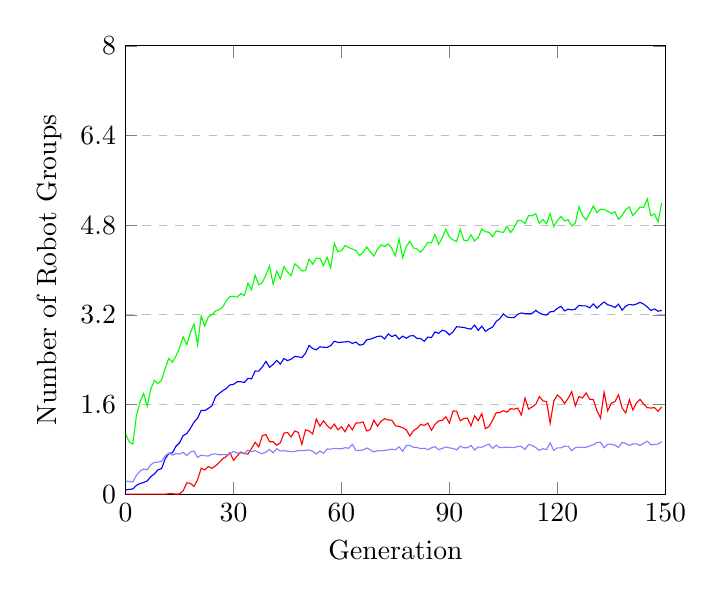
\begin{tikzpicture}
\begin{axis}[
	xlabel={Generation},
	ylabel={Number of Robot Groups},
	xmin=0, xmax=150,
	ymin=0, ymax=8,
	xtick={0.0,30.0,60.0,90.0,120.0,150.0},
	ytick={0.0,1.6,3.2,4.800000000000001,6.4,8.0},
	ymajorgrids=true,
	grid style=dashed,
]

\addplot[
	color=green,
	]
	coordinates {
	(0,1.0766666666666664)(1,0.9317500000000001)(2,0.8944166666666665)(3,1.4018333333333333)(4,1.6415)(5,1.7967499999999998)(6,1.5664166666666666)(7,1.8767499999999995)(8,2.0290833333333333)(9,1.9709999999999999)(10,2.0363333333333333)(11,2.244333333333333)(12,2.42275)(13,2.353833333333333)(14,2.46375)(15,2.6136666666666666)(16,2.8068333333333326)(17,2.6658333333333335)(18,2.8832500000000003)(19,3.034583333333333)(20,2.6674999999999995)(21,3.1786666666666665)(22,2.999833333333333)(23,3.1666666666666665)(24,3.200416666666667)(25,3.266833333333333)(26,3.290333333333333)(27,3.3386666666666667)(28,3.4558333333333335)(29,3.5255833333333335)(30,3.526500000000001)(31,3.514000000000001)(32,3.5758333333333328)(33,3.545)(34,3.7640000000000002)(35,3.6470000000000002)(36,3.908416666666667)(37,3.7350000000000003)(38,3.774166666666667)(39,3.914916666666666)(40,4.069583333333333)(41,3.743833333333334)(42,3.978333333333334)(43,3.83775)(44,4.060250000000001)(45,3.9614166666666666)(46,3.8988333333333336)(47,4.110166666666666)(48,4.05775)(49,3.982333333333333)(50,3.9917499999999997)(51,4.195166666666667)(52,4.101583333333332)(53,4.213166666666667)(54,4.205583333333333)(55,4.076833333333333)(56,4.228083333333333)(57,4.034083333333333)(58,4.4760833333333325)(59,4.329416666666667)(60,4.344416666666667)(61,4.43575)(62,4.402416666666666)(63,4.3726666666666665)(64,4.348166666666667)(65,4.255)(66,4.3148333333333335)(67,4.411833333333332)(68,4.324916666666667)(69,4.247583333333334)(70,4.37025)(71,4.449333333333334)(72,4.419333333333333)(73,4.465000000000001)(74,4.384583333333333)(75,4.253083333333333)(76,4.553916666666666)(77,4.219416666666667)(78,4.421916666666667)(79,4.5115)(80,4.394666666666667)(81,4.374250000000001)(82,4.31675)(83,4.398000000000001)(84,4.489916666666667)(85,4.485333333333332)(86,4.632083333333333)(87,4.457583333333332)(88,4.571333333333334)(89,4.73075)(90,4.588916666666667)(91,4.536583333333334)(92,4.507416666666665)(93,4.730583333333334)(94,4.5315)(95,4.519333333333333)(96,4.628583333333333)(97,4.516749999999999)(98,4.578583333333333)(99,4.731416666666666)(100,4.683583333333333)(101,4.670333333333333)(102,4.593666666666666)(103,4.698833333333334)(104,4.6814166666666654)(105,4.670833333333334)(106,4.779083333333334)(107,4.6656666666666675)(108,4.7555)(109,4.884833333333334)(110,4.879333333333334)(111,4.83075)(112,4.970083333333332)(113,4.966666666666667)(114,5.003750000000001)(115,4.827916666666668)(116,4.901166666666667)(117,4.8267500000000005)(118,5.004833333333334)(119,4.774333333333334)(120,4.8812500000000005)(121,4.955833333333334)(122,4.874333333333333)(123,4.896333333333334)(124,4.785416666666666)(125,4.837083333333332)(126,5.128166666666668)(127,4.967666666666665)(128,4.892666666666666)(129,5.01525)(130,5.144166666666666)(131,5.022833333333334)(132,5.0840000000000005)(133,5.080166666666666)(134,5.0480833333333335)(135,5.008916666666666)(136,5.0365)(137,4.902333333333333)(138,4.974166666666667)(139,5.075166666666667)(140,5.125416666666667)(141,4.971166666666668)(142,5.042083333333333)(143,5.125416666666667)(144,5.11175)(145,5.267166666666667)(146,4.9695833333333335)(147,4.996666666666667)(148,4.857500000000001)(149,5.191833333333332)
	};
\addplot[
	color=blue,
	]
	coordinates {
	(0,0.07716666666666666)(1,0.08356944444444443)(2,0.09260416666666665)(3,0.15574999999999997)(4,0.1885902777777778)(5,0.20923611111111115)(6,0.23522916666666668)(7,0.3124687500000001)(8,0.36154861111111103)(9,0.43432638888888897)(10,0.4570069444444444)(11,0.6308541666666666)(12,0.7261076388888889)(13,0.7383576388888888)(14,0.8549444444444444)(15,0.918545138888889)(16,1.0449027777777777)(17,1.0812291666666665)(18,1.1721736111111114)(19,1.2848819444444444)(20,1.3564479166666668)(21,1.4950555555555556)(22,1.4918750000000005)(23,1.5310000000000004)(24,1.577090277777778)(25,1.7403576388888888)(26,1.7960763888888887)(27,1.8458402777777778)(28,1.8858368055555554)(29,1.9494687499999996)(30,1.95853125)(31,2.0055729166666665)(32,2.0067013888888887)(33,1.992236111111111)(34,2.0640312499999993)(35,2.0572222222222227)(36,2.196916666666666)(37,2.1944930555555557)(38,2.270201388888889)(39,2.368940972222222)(40,2.263479166666666)(41,2.3142604166666665)(42,2.387767361111111)(43,2.320732638888889)(44,2.419388888888889)(45,2.3829305555555558)(46,2.407756944444444)(47,2.456572916666667)(48,2.450177083333334)(49,2.4354340277777777)(50,2.513722222222223)(51,2.654177083333334)(52,2.596510416666666)(53,2.5772673611111117)(54,2.6275104166666656)(55,2.62115625)(56,2.617649305555555)(57,2.649947916666666)(58,2.728420138888889)(59,2.7065034722222228)(60,2.7109027777777777)(61,2.7174965277777776)(62,2.722170138888889)(63,2.689701388888889)(64,2.7126597222222224)(65,2.6592083333333334)(66,2.6692916666666666)(67,2.7526006944444443)(68,2.765520833333334)(69,2.7883159722222213)(70,2.8140833333333326)(71,2.820479166666667)(72,2.7687777777777773)(73,2.8595243055555555)(74,2.8109791666666673)(75,2.8399513888888888)(76,2.765788194444445)(77,2.8198645833333336)(78,2.782503472222222)(79,2.8221145833333328)(80,2.8287326388888885)(81,2.7777048611111117)(82,2.775878472222222)(83,2.7273194444444444)(84,2.8030243055555553)(85,2.794791666666667)(86,2.8952291666666663)(87,2.867625)(88,2.926517361111111)(89,2.9045937500000005)(90,2.8414236111111113)(91,2.896010416666667)(92,2.9868541666666673)(93,2.9814097222222222)(94,2.974350694444444)(95,2.956309027777778)(96,2.9440208333333335)(97,3.0166006944444437)(98,2.921309027777777)(99,2.9973125)(100,2.905086805555555)(101,2.9483333333333337)(102,2.981375)(103,3.0809618055555554)(104,3.1299027777777777)(105,3.2150798611111115)(106,3.1622812499999995)(107,3.1503402777777776)(108,3.1505937500000005)(109,3.2114444444444437)(110,3.2324305555555557)(111,3.222177083333334)(112,3.2174305555555556)(113,3.2243993055555564)(114,3.278503472222222)(115,3.2329166666666667)(116,3.2047361111111115)(117,3.1939791666666664)(118,3.2531909722222223)(119,3.2600486111111118)(120,3.3147812500000002)(121,3.351545138888888)(122,3.269107638888889)(123,3.3010416666666673)(124,3.2865868055555563)(125,3.3006284722222223)(126,3.3676111111111102)(127,3.359447916666667)(128,3.3589791666666664)(129,3.3244201388888888)(130,3.3944513888888896)(131,3.319916666666666)(132,3.3766666666666665)(133,3.4287222222222216)(134,3.3795104166666667)(135,3.3624652777777775)(136,3.329680555555555)(137,3.3896562500000003)(138,3.2812361111111112)(139,3.3538819444444448)(140,3.3867847222222225)(141,3.3738263888888897)(142,3.3926562499999995)(143,3.4229444444444437)(144,3.390142361111111)(145,3.33909375)(146,3.2779722222222216)(147,3.3053437500000005)(148,3.2630243055555552)(149,3.278666666666667)
	};
\addplot[
	color=red,
	]
	coordinates {
	(0,0.0)(1,0.0)(2,0.0)(3,0.0)(4,0.0)(5,0.0)(6,0.0)(7,0.0)(8,0.0)(9,0.0)(10,0.0001666666666666667)(11,0.00041666666666666664)(12,0.007083333333333333)(13,0.008000000000000002)(14,0.0008333333333333333)(15,0.0041666666666666675)(16,0.060416666666666674)(17,0.2004166666666667)(18,0.19224999999999998)(19,0.1375)(20,0.25675)(21,0.46275)(22,0.4303333333333333)(23,0.4940833333333332)(24,0.4609166666666667)(25,0.50575)(26,0.56375)(27,0.6324166666666667)(28,0.6723333333333333)(29,0.7375)(30,0.6014166666666667)(31,0.6811666666666667)(32,0.7515833333333334)(33,0.72025)(34,0.7166666666666668)(35,0.8160000000000001)(36,0.9246666666666667)(37,0.8435833333333331)(38,1.0433333333333332)(39,1.0645833333333334)(40,0.93475)(41,0.9356666666666666)(42,0.87275)(43,0.9153333333333333)(44,1.088583333333333)(45,1.1005833333333332)(46,1.02025)(47,1.1260833333333329)(48,1.1016666666666668)(49,0.8888333333333334)(50,1.1480833333333333)(51,1.1261666666666668)(52,1.0735000000000001)(53,1.3421666666666672)(54,1.2116666666666667)(55,1.3088333333333333)(56,1.2244999999999997)(57,1.1654166666666665)(58,1.2509166666666667)(59,1.1485)(60,1.2000833333333336)(61,1.114)(62,1.2414999999999998)(63,1.1468333333333331)(64,1.2687500000000003)(65,1.2712500000000002)(66,1.2883333333333333)(67,1.1267500000000001)(68,1.1508333333333334)(69,1.3215000000000001)(70,1.2143333333333335)(71,1.3000833333333333)(72,1.3466666666666667)(73,1.3238333333333334)(74,1.3181666666666665)(75,1.2203333333333333)(76,1.20925)(77,1.1845)(78,1.1491666666666667)(79,1.0354166666666667)(80,1.132666666666667)(81,1.1747500000000002)(82,1.2450833333333333)(83,1.2251666666666667)(84,1.266666666666667)(85,1.1382499999999998)(86,1.2446666666666666)(87,1.30675)(88,1.3151666666666666)(89,1.3789166666666668)(90,1.2670833333333333)(91,1.4848333333333337)(92,1.481)(93,1.3084166666666668)(94,1.34925)(95,1.3569166666666668)(96,1.2179166666666665)(97,1.3965833333333335)(98,1.3112499999999998)(99,1.4375000000000004)(100,1.1683333333333334)(101,1.206333333333333)(102,1.31875)(103,1.4514999999999998)(104,1.4555833333333332)(105,1.4911666666666665)(106,1.462416666666667)(107,1.524833333333333)(108,1.515416666666667)(109,1.53475)(110,1.4115000000000002)(111,1.7159999999999995)(112,1.5177500000000002)(113,1.5575)(114,1.6021666666666667)(115,1.7412500000000002)(116,1.6633333333333333)(117,1.6514999999999995)(118,1.2639166666666666)(119,1.6592499999999997)(120,1.7700000000000002)(121,1.7139166666666668)(122,1.6175833333333336)(123,1.7083333333333333)(124,1.8313333333333335)(125,1.5742500000000001)(126,1.741666666666667)(127,1.7166666666666668)(128,1.8074166666666667)(129,1.6929999999999998)(130,1.6857500000000003)(131,1.4923333333333333)(132,1.3565833333333335)(133,1.81825)(134,1.4871666666666667)(135,1.6244999999999996)(136,1.6499166666666665)(137,1.7729166666666663)(138,1.5373333333333334)(139,1.4484166666666665)(140,1.6869999999999998)(141,1.4997500000000004)(142,1.6291666666666667)(143,1.6901666666666666)(144,1.6049166666666668)(145,1.5425833333333332)(146,1.5356666666666665)(147,1.5442499999999997)(148,1.4778333333333333)(149,1.557166666666667)
	};
\addplot[
	color=blue!50,
	]
	coordinates {
	(0,0.2358219876621716)(1,0.22409786643074095)(2,0.21768762215620266)(3,0.3360418961237025)(4,0.4104290604839639)(5,0.4477558247582203)(6,0.43332953023789134)(7,0.5251991583824773)(8,0.5668023555191838)(9,0.5714508535401401)(10,0.5862499182507215)(11,0.6822144380527035)(12,0.7312344217652115)(13,0.6963535841821741)(14,0.7233151996124794)(15,0.716191937951961)(16,0.7467032737341078)(17,0.6861730171192848)(18,0.7524781458040856)(19,0.7700498804937517)(20,0.6535684007081176)(21,0.6966217738611062)(22,0.6844602709971597)(23,0.6800974811152077)(24,0.7123903090259056)(25,0.7186879415658306)(26,0.7019796188027463)(27,0.7058235705229318)(28,0.702290133707745)(29,0.7158476040990822)(30,0.7643517711602652)(31,0.7333463092041888)(32,0.735930369592371)(33,0.7265738180825504)(34,0.7859092901484073)(35,0.7590894363643593)(36,0.7774435909634844)(37,0.7429812941191432)(38,0.7232742696775717)(39,0.7506873441675904)(40,0.7978478856512301)(41,0.7368132529544781)(42,0.8108729722891899)(43,0.7697241759762005)(44,0.7767530573768086)(45,0.7658480003042184)(46,0.7581970218803556)(47,0.762236251813436)(48,0.7793241147374186)(49,0.77531520777878)(50,0.7813488179342017)(51,0.7883504269377107)(52,0.7640280243197508)(53,0.7168474274647983)(54,0.7688486898320419)(55,0.7285129274556265)(56,0.807114261798217)(57,0.801505666601279)(58,0.8164172638861603)(59,0.8127570014144722)(60,0.8077645227261571)(61,0.8293650337695446)(62,0.8179323190927504)(63,0.8893486108335483)(64,0.7793454329727876)(65,0.7811321708609763)(66,0.7867093845220872)(67,0.8240625050061796)(68,0.7890651866581161)(69,0.7527666598636116)(70,0.7741750892091797)(71,0.7716609242731948)(72,0.7808207060964029)(73,0.7885075854287684)(74,0.8022824890640615)(75,0.7926827274039769)(76,0.844886079489975)(77,0.7652722272893019)(78,0.8684308258914485)(79,0.870513450485844)(80,0.8339179167393219)(81,0.8342328432516622)(82,0.8117807688361038)(83,0.8184023730148613)(84,0.7940009858296574)(85,0.8265165036060065)(86,0.8471576477971966)(87,0.7934990134995605)(88,0.8157438161217173)(89,0.8405780070285194)(90,0.8254038490758994)(91,0.8157830732688575)(92,0.7895773060380056)(93,0.8545317864123545)(94,0.8271912833569836)(95,0.8266873532065764)(96,0.8686751636542279)(97,0.7869734101313398)(98,0.8407722601124658)(99,0.8359104680021475)(100,0.8690218598542834)(101,0.8913086099721522)(102,0.8164613396206198)(103,0.8738887194828214)(104,0.8285469114167987)(105,0.8336971692751902)(106,0.8386101559019568)(107,0.8309872657761602)(108,0.8308668931669366)(109,0.8523073182059595)(110,0.848357687310758)(111,0.7987849644604984)(112,0.8847177868615094)(113,0.8683654010140945)(114,0.8298310176774799)(115,0.7810621533808734)(116,0.8111842799487909)(117,0.7943244905520549)(118,0.9148158388152091)(119,0.7786115055627179)(120,0.8264680511772847)(121,0.8256672960015233)(122,0.8546300556204514)(123,0.8569347557045202)(124,0.7744461286556957)(125,0.82872376021537)(126,0.840044958541895)(127,0.8324991893108769)(128,0.8373467145682034)(129,0.8596906751090491)(130,0.8798747956597368)(131,0.9217468963082962)(132,0.9261402060085171)(133,0.8283809277968154)(134,0.8920342492322417)(135,0.8903019163284567)(136,0.8735390292657276)(137,0.8359263039406146)(138,0.9242499785973742)(139,0.9039492605526912)(140,0.8690759325959957)(141,0.893498272595738)(142,0.898657691580899)(143,0.8688484014595504)(144,0.9099585958874736)(145,0.9456881792455814)(146,0.8793025129775671)(147,0.8865304640893338)(148,0.8951390635165519)(149,0.9357362907022126)
	};
\end{axis}
\end{tikzpicture}
}
		\caption{Some sample caption}
	\end{subfigure}%
}
\\
\\
\\
\\
	\makebox[\linewidth][c]{%
	\begin{subfigure}[b]{0.7\textwidth}
		\centering
		\resizebox{0.9\linewidth}{!}{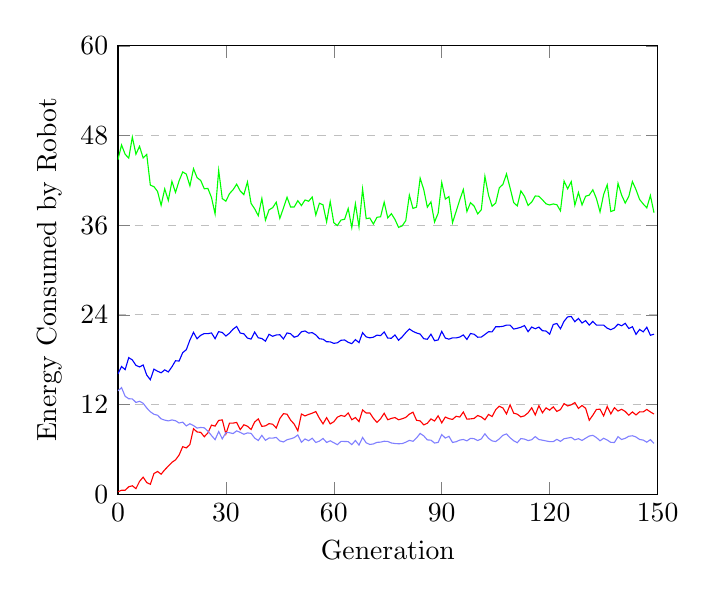
\begin{tikzpicture}
\begin{axis}[
	xlabel={Generation},
	ylabel={Energy Consumed by Robot},
	xmin=0, xmax=150,
	ymin=0, ymax=60,
	xtick={0.0,30.0,60.0,90.0,120.0,150.0},
	ytick={0.0,12.0,24.0,36.0,48.0,60.0},
	ymajorgrids=true,
	grid style=dashed,
]

\addplot[
	color=green,
	]
	coordinates {
	(0,44.74999999999999)(1,46.733333333333334)(2,45.48333333333334)(3,44.96666666666666)(4,47.783333333333324)(5,45.49999999999999)(6,46.55)(7,44.99999999999999)(8,45.46666666666667)(9,41.35000000000001)(10,41.14999999999999)(11,40.51666666666666)(12,38.65)(13,40.849999999999994)(14,39.3)(15,41.849999999999994)(16,40.38333333333333)(17,41.93333333333334)(18,43.11666666666667)(19,42.83333333333333)(20,41.25000000000001)(21,43.550000000000004)(22,42.349999999999994)(23,41.983333333333334)(24,40.866666666666674)(25,40.91666666666667)(26,39.70000000000001)(27,37.49999999999999)(28,43.33333333333334)(29,39.550000000000004)(30,39.20000000000001)(31,40.21666666666667)(32,40.733333333333334)(33,41.48333333333333)(34,40.56666666666666)(35,40.08333333333333)(36,41.78333333333333)(37,38.91666666666667)(38,38.18333333333332)(39,37.26666666666667)(40,39.56666666666666)(41,36.66666666666667)(42,38.050000000000004)(43,38.333333333333336)(44,39.066666666666656)(45,36.9)(46,38.28333333333334)(47,39.733333333333334)(48,38.41666666666667)(49,38.43333333333333)(50,39.266666666666666)(51,38.61666666666667)(52,39.366666666666674)(53,39.2)(54,39.76666666666667)(55,37.35)(56,38.93333333333333)(57,38.71666666666667)(58,36.43333333333333)(59,39.150000000000006)(60,36.31666666666667)(61,35.949999999999996)(62,36.68333333333333)(63,36.78333333333333)(64,38.21666666666666)(65,35.66666666666667)(66,38.866666666666674)(67,35.766666666666666)(68,40.83333333333334)(69,36.86666666666666)(70,36.95000000000001)(71,36.15)(72,37.050000000000004)(73,37.11666666666667)(74,39.08333333333333)(75,36.96666666666667)(76,37.53333333333333)(77,36.76666666666667)(78,35.7)(79,35.900000000000006)(80,36.6)(81,40.01666666666667)(82,38.233333333333334)(83,38.41666666666667)(84,42.28333333333333)(85,40.76666666666667)(86,38.400000000000006)(87,39.116666666666674)(88,36.416666666666664)(89,37.583333333333336)(90,41.71666666666666)(91,39.483333333333334)(92,39.81666666666666)(93,36.333333333333336)(94,37.833333333333336)(95,39.366666666666674)(96,40.766666666666666)(97,37.81666666666666)(98,39.016666666666666)(99,38.55)(100,37.5)(101,38.06666666666667)(102,42.53333333333334)(103,40.033333333333324)(104,38.53333333333333)(105,38.95)(106,41.0)(107,41.449999999999996)(108,42.85)(109,40.96666666666667)(110,39.01666666666667)(111,38.56666666666666)(112,40.583333333333336)(113,39.86666666666666)(114,38.63333333333333)(115,39.083333333333336)(116,39.9)(117,39.86666666666665)(118,39.38333333333333)(119,38.85)(120,38.699999999999996)(121,38.83333333333333)(122,38.73333333333334)(123,37.91666666666666)(124,41.900000000000006)(125,40.866666666666674)(126,41.833333333333336)(127,38.666666666666664)(128,40.36666666666667)(129,38.7)(130,39.86666666666667)(131,40.016666666666666)(132,40.733333333333334)(133,39.55)(134,37.766666666666666)(135,40.10000000000001)(136,41.4)(137,37.81666666666666)(138,38.0)(139,41.6)(140,40.01666666666667)(141,38.94999999999999)(142,39.85)(143,41.83333333333333)(144,40.75)(145,39.43333333333333)(146,38.83333333333333)(147,38.31666666666666)(148,39.96666666666667)(149,37.666666666666664)
	};
\addplot[
	color=blue,
	]
	coordinates {
	(0,16.090972222222224)(1,17.07847222222222)(2,16.659722222222225)(3,18.26875)(4,17.955555555555556)(5,17.243055555555554)(6,17.01597222222222)(7,17.287499999999998)(8,15.933333333333332)(9,15.311111111111112)(10,16.726388888888888)(11,16.452777777777776)(12,16.236111111111114)(13,16.63125)(14,16.35138888888889)(15,17.035416666666666)(16,17.84722222222222)(17,17.809027777777775)(18,18.93333333333333)(19,19.32847222222222)(20,20.615277777777777)(21,21.64652777777778)(22,20.788888888888895)(23,21.256250000000005)(24,21.48472222222222)(25,21.475694444444443)(26,21.571527777777778)(27,20.807638888888892)(28,21.747222222222224)(29,21.62916666666667)(30,21.15694444444445)(31,21.538194444444446)(32,22.079166666666666)(33,22.441666666666666)(34,21.55486111111111)(35,21.456249999999997)(36,20.881944444444443)(37,20.746527777777775)(38,21.684027777777775)(39,20.920833333333338)(40,20.82361111111111)(41,20.46944444444444)(42,21.38888888888889)(43,21.122222222222224)(44,21.29861111111111)(45,21.330555555555556)(46,20.768749999999997)(47,21.574305555555558)(48,21.464583333333337)(49,20.999999999999996)(50,21.163194444444446)(51,21.724305555555556)(52,21.835416666666667)(53,21.54722222222222)(54,21.614583333333332)(55,21.306249999999995)(56,20.793750000000003)(57,20.736111111111114)(58,20.395833333333336)(59,20.376388888888886)(60,20.177777777777777)(61,20.259027777777778)(62,20.58680555555556)(63,20.632638888888888)(64,20.308333333333334)(65,20.142361111111107)(66,20.67638888888889)(67,20.279166666666665)(68,21.608333333333338)(69,21.04236111111111)(70,20.914583333333333)(71,21.000694444444445)(72,21.279861111111114)(73,21.207638888888884)(74,21.709027777777774)(75,20.871527777777775)(76,20.865972222222222)(77,21.30138888888889)(78,20.58472222222222)(79,21.042361111111113)(80,21.610416666666666)(81,22.105555555555554)(82,21.781249999999996)(83,21.566666666666666)(84,21.42083333333333)(85,20.797222222222224)(86,20.727083333333336)(87,21.402777777777775)(88,20.532638888888886)(89,20.62986111111111)(90,21.78055555555556)(91,20.881250000000005)(92,20.7375)(93,20.915972222222223)(94,20.904861111111114)(95,21.022916666666674)(96,21.304861111111105)(97,20.704861111111114)(98,21.492361111111112)(99,21.395138888888887)(100,20.999999999999996)(101,21.016666666666666)(102,21.363194444444442)(103,21.727777777777778)(104,21.719444444444438)(105,22.393750000000008)(106,22.39861111111111)(107,22.455555555555556)(108,22.620833333333337)(109,22.615277777777774)(110,22.089583333333334)(111,22.195138888888888)(112,22.333333333333332)(113,22.559722222222224)(114,21.739583333333332)(115,22.357638888888886)(116,22.132638888888888)(117,22.350694444444436)(118,21.87222222222222)(119,21.822222222222226)(120,21.406249999999996)(121,22.703472222222224)(122,22.836111111111112)(123,22.126388888888883)(124,23.135416666666664)(125,23.720138888888894)(126,23.77430555555555)(127,23.07430555555556)(128,23.511111111111116)(129,22.89652777777778)(130,23.218055555555555)(131,22.61527777777778)(132,23.120138888888885)(133,22.62777777777778)(134,22.609027777777783)(135,22.620833333333337)(136,22.204861111111114)(137,22.002777777777773)(138,22.243055555555554)(139,22.743055555555554)(140,22.52986111111111)(141,22.860416666666673)(142,22.162499999999998)(143,22.41111111111111)(144,21.38263888888889)(145,22.039583333333333)(146,21.71527777777778)(147,22.33611111111112)(148,21.257638888888884)(149,21.402777777777782)
	};
\addplot[
	color=red,
	]
	coordinates {
	(0,0.31666666666666665)(1,0.5166666666666666)(2,0.5166666666666667)(3,0.9833333333333336)(4,1.116666666666667)(5,0.7333333333333333)(6,1.7000000000000004)(7,2.2666666666666666)(8,1.5500000000000003)(9,1.3166666666666667)(10,2.7499999999999996)(11,3.033333333333333)(12,2.666666666666667)(13,3.25)(14,3.7499999999999996)(15,4.25)(16,4.583333333333333)(17,5.233333333333333)(18,6.35)(19,6.183333333333334)(20,6.6499999999999995)(21,8.75)(22,8.316666666666666)(23,8.266666666666667)(24,7.683333333333335)(25,8.183333333333334)(26,9.233333333333336)(27,9.1)(28,9.866666666666667)(29,9.933333333333332)(30,8.049999999999999)(31,9.5)(32,9.500000000000004)(33,9.600000000000001)(34,8.633333333333333)(35,9.283333333333333)(36,9.083333333333334)(37,8.649999999999999)(38,9.65)(39,10.066666666666666)(40,9.066666666666666)(41,9.133333333333333)(42,9.433333333333335)(43,9.350000000000001)(44,8.850000000000001)(45,10.116666666666669)(46,10.766666666666667)(47,10.7)(48,9.9)(49,9.366666666666665)(50,8.466666666666667)(51,10.716666666666667)(52,10.466666666666667)(53,10.666666666666668)(54,10.833333333333334)(55,11.05)(56,10.149999999999999)(57,9.399999999999999)(58,10.233333333333333)(59,9.4)(60,9.683333333333334)(61,10.299999999999999)(62,10.533333333333333)(63,10.4)(64,10.866666666666667)(65,9.95)(66,10.25)(67,9.700000000000001)(68,11.26666666666667)(69,10.85)(70,10.866666666666664)(71,10.149999999999999)(72,9.6)(73,10.083333333333334)(74,10.816666666666668)(75,9.950000000000001)(76,10.133333333333333)(77,10.250000000000002)(78,9.95)(79,10.083333333333332)(80,10.266666666666662)(81,10.700000000000001)(82,10.966666666666667)(83,9.883333333333331)(84,9.799999999999999)(85,9.266666666666667)(86,9.483333333333334)(87,10.066666666666668)(88,9.783333333333335)(89,10.483333333333334)(90,9.533333333333333)(91,10.316666666666665)(92,10.099999999999998)(93,9.999999999999998)(94,10.416666666666666)(95,10.316666666666666)(96,10.983333333333333)(97,10.033333333333331)(98,10.066666666666666)(99,10.133333333333333)(100,10.516666666666666)(101,10.333333333333334)(102,9.950000000000001)(103,10.666666666666666)(104,10.383333333333335)(105,11.299999999999999)(106,11.766666666666667)(107,11.533333333333333)(108,10.73333333333333)(109,11.95)(110,10.833333333333336)(111,10.7)(112,10.333333333333332)(113,10.483333333333333)(114,10.883333333333333)(115,11.549999999999999)(116,10.6)(117,11.833333333333332)(118,10.883333333333333)(119,11.55)(120,11.233333333333333)(121,11.68333333333333)(122,11.066666666666666)(123,11.316666666666666)(124,12.116666666666665)(125,11.8)(126,11.949999999999998)(127,12.25)(128,11.466666666666667)(129,11.866666666666665)(130,11.483333333333334)(131,9.883333333333335)(132,10.566666666666666)(133,11.333333333333332)(134,11.366666666666669)(135,10.466666666666667)(136,11.73333333333333)(137,10.733333333333336)(138,11.566666666666666)(139,11.116666666666667)(140,11.350000000000001)(141,11.066666666666668)(142,10.566666666666666)(143,11.0)(144,10.6)(145,11.016666666666664)(146,11.0)(147,11.333333333333337)(148,11.0)(149,10.716666666666665)
	};
\addplot[
	color=blue!50,
	]
	coordinates {
	(0,13.819806599360406)(1,14.250737907236743)(2,13.093433621408368)(3,12.763356786049899)(4,12.74368488937983)(5,12.271179086369875)(6,12.42502499101579)(7,12.159044049031039)(8,11.532071599560236)(9,11.023136218277813)(10,10.688280972623168)(11,10.557264862529339)(12,10.073085003700253)(13,9.903527118007691)(14,9.799710623720102)(15,9.927769579013912)(16,9.82531594821428)(17,9.518316244203994)(18,9.631192077001366)(19,9.131396958977227)(20,9.417911400843225)(21,9.1748768378596)(22,8.836709140225913)(23,8.922007966526804)(24,8.872690995096375)(25,8.43248300614129)(26,7.843523041073483)(27,7.2909868544594385)(28,8.370068086407823)(29,7.398162037841813)(30,8.22051614831994)(31,8.220794543270543)(32,8.10298888060539)(33,8.465702832564082)(34,8.262108547055336)(35,8.012595874518665)(36,8.193428014915943)(37,8.132940041590745)(38,7.5084614260160985)(39,7.173748233504123)(40,7.867475616380679)(41,7.199851685815094)(42,7.509063818853958)(43,7.492504854036616)(44,7.594923713356814)(45,7.120038059372446)(46,6.9817987738353136)(47,7.275799710705311)(48,7.401115669947693)(49,7.565759965283135)(50,7.924157867244477)(51,6.940532437702562)(52,7.377349126643417)(53,7.145697634484754)(54,7.478741916788094)(55,6.906790085478266)(56,7.096408179221382)(57,7.447372094478278)(58,6.916081258523769)(59,7.136741691941585)(60,6.876224510654938)(61,6.623894900769512)(62,7.062730721520471)(63,7.043473656790395)(64,7.029241917042987)(65,6.622218645433792)(66,7.182830278018752)(67,6.56286553159204)(68,7.581791799805685)(69,6.867039853602438)(70,6.6476467356478)(71,6.7160856230295565)(72,6.930133864873364)(73,6.956045929448708)(74,7.076154622258886)(75,7.04820123922273)(76,6.844647201926222)(77,6.770677551493188)(78,6.739627613986846)(79,6.761311355226734)(80,6.942085859506217)(81,7.197808430021265)(82,7.070445599977569)(83,7.521139229378491)(84,8.122353002322837)(85,7.793844372311219)(86,7.255862105239233)(87,7.223138541212654)(88,6.836135266370989)(89,6.915127216208116)(90,7.971759322038431)(91,7.499741438596823)(92,7.7386518883050055)(93,6.913631259373276)(94,7.010906410724734)(95,7.233722060379922)(96,7.310030552700287)(97,7.1293560099612225)(98,7.464556147968515)(99,7.419020636927533)(100,7.169525352498313)(101,7.3901939537832355)(102,8.07517676360289)(103,7.461075035761211)(104,7.120946788737036)(105,7.038006165467384)(106,7.396056049186398)(107,7.869980823314177)(108,8.0576291950702)(109,7.538410336362136)(110,7.144754630839188)(111,6.882322982549827)(112,7.435295099008024)(113,7.366927363763599)(114,7.163787335787269)(115,7.276864219803643)(116,7.7005482152488165)(117,7.305767426823847)(118,7.2177388045249415)(119,7.116882757472325)(120,7.027073234309885)(121,7.023559805724868)(122,7.331115921904532)(123,7.057236927902183)(124,7.411373581887798)(125,7.501616129582619)(126,7.595024947345743)(127,7.264882138383145)(128,7.416882994086323)(129,7.184639979510641)(130,7.486178834373604)(131,7.7726052055357)(132,7.867497257484729)(133,7.565689898649469)(134,7.137854780743645)(135,7.474534980271977)(136,7.239504283216544)(137,6.921046602357998)(138,6.911602044811234)(139,7.6900991279050075)(140,7.3062844504979925)(141,7.465372337131035)(142,7.741354206395464)(143,7.807663319048861)(144,7.643325311931658)(145,7.312268531584327)(146,7.235158167806764)(147,6.948607530515565)(148,7.29493731218281)(149,6.791561892771329)
	};
\end{axis}
\end{tikzpicture}
}
		\caption{Some sample caption}
	\end{subfigure}%
	\begin{subfigure}[b]{0.7\textwidth}
		\centering
		\resizebox{0.9\linewidth}{!}{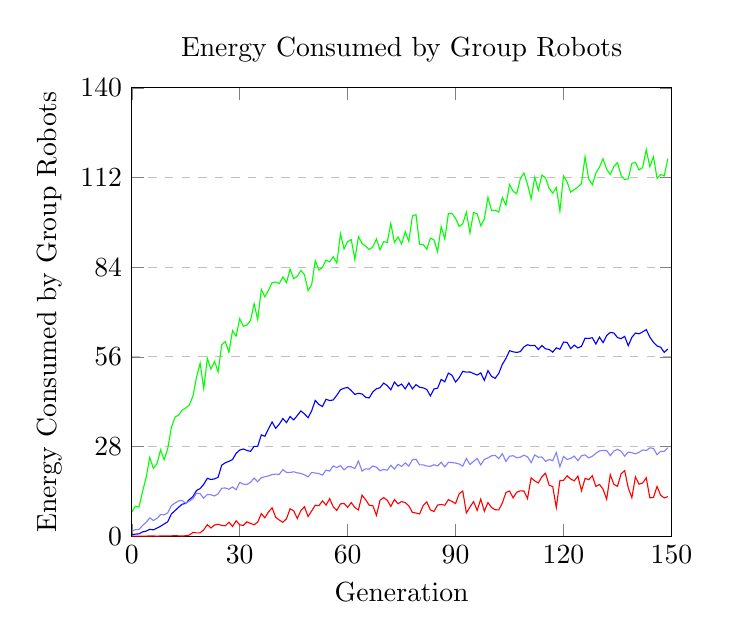
\begin{tikzpicture}
\begin{axis}[
	title={Energy Consumed by Group Robots},
	xlabel={Generation},
	ylabel={Energy Consumed by Group Robots},
	xmin=0, xmax=150,
	ymin=0, ymax=140,
	xtick={0.0,30.0,60.0,90.0,120.0,150.0},
	ytick={0.0,28.0,56.0,84.0,112.0,140.0},
	ymajorgrids=true,
	grid style=dashed,
]

\addplot[
	color=green,
	]
	coordinates {
	(0,7.550000000000001)(1,9.333333333333336)(2,9.100000000000001)(3,13.933333333333335)(4,18.383333333333336)(5,24.600000000000005)(6,21.166666666666668)(7,22.649999999999995)(8,26.933333333333334)(9,23.883333333333336)(10,27.4)(11,33.916666666666664)(12,37.166666666666664)(13,37.81666666666667)(14,39.36666666666667)(15,39.999999999999986)(16,41.01666666666666)(17,43.78333333333334)(18,49.666666666666664)(19,54.08333333333333)(20,46.06666666666668)(21,55.51666666666667)(22,52.2)(23,54.56666666666666)(24,51.31666666666667)(25,59.76666666666666)(26,60.783333333333324)(27,57.41666666666667)(28,64.21666666666667)(29,62.48333333333333)(30,67.91666666666667)(31,65.56666666666665)(32,65.91666666666666)(33,67.38333333333334)(34,72.60000000000001)(35,67.63333333333334)(36,77.08333333333334)(37,74.73333333333333)(38,76.8)(39,79.21666666666667)(40,79.36666666666667)(41,78.9)(42,80.91666666666666)(43,79.16666666666667)(44,83.39999999999999)(45,80.43333333333332)(46,81.13333333333331)(47,82.99999999999997)(48,81.66666666666669)(49,76.68333333333334)(50,78.5)(51,86.05)(52,83.10000000000001)(53,83.95000000000002)(54,86.23333333333332)(55,85.68333333333332)(56,87.28333333333333)(57,85.28333333333333)(58,94.41666666666666)(59,89.69999999999999)(60,91.98333333333332)(61,92.63333333333333)(62,86.43333333333334)(63,93.54999999999998)(64,91.46666666666667)(65,90.56666666666665)(66,89.53333333333332)(67,90.35)(68,92.8166666666667)(69,89.41666666666666)(70,91.99999999999999)(71,91.68333333333334)(72,97.68333333333335)(73,91.75000000000001)(74,93.45)(75,91.25)(76,95.08333333333336)(77,92.03333333333335)(78,100.0)(79,100.43333333333331)(80,91.15)(81,91.10000000000001)(82,89.55)(83,93.10000000000001)(84,92.5)(85,88.79999999999998)(86,96.73333333333332)(87,92.78333333333335)(88,100.7)(89,100.73333333333333)(90,99.23333333333335)(91,96.7)(92,97.61666666666667)(93,101.18333333333331)(94,94.68333333333332)(95,101.08333333333334)(96,100.68333333333337)(97,96.94999999999997)(98,99.06666666666669)(99,105.8)(100,101.68333333333334)(101,101.78333333333333)(102,101.21666666666665)(103,105.76666666666665)(104,103.40000000000002)(105,109.81666666666665)(106,107.75)(107,106.94999999999999)(108,111.63333333333333)(109,113.4)(110,109.8833333333333)(111,105.33333333333334)(112,112.10000000000001)(113,108.05000000000001)(114,112.78333333333332)(115,111.85)(116,108.61666666666665)(117,107.11666666666666)(118,108.9)(119,101.51666666666665)(120,112.5333333333333)(121,110.63333333333334)(122,107.41666666666666)(123,108.23333333333333)(124,109.03333333333335)(125,110.13333333333335)(126,118.48333333333335)(127,111.55)(128,109.76666666666667)(129,113.38333333333333)(130,115.25000000000001)(131,117.86666666666667)(132,114.51666666666668)(133,112.96666666666667)(134,115.41666666666669)(135,116.63333333333335)(136,112.7)(137,111.36666666666666)(138,111.60000000000001)(139,116.43333333333334)(140,116.71666666666667)(141,114.36666666666667)(142,115.13333333333331)(143,120.71666666666667)(144,115.38333333333334)(145,118.48333333333333)(146,111.75000000000001)(147,112.93333333333331)(148,112.53333333333332)(149,117.89999999999998)
	};
\addplot[
	color=blue,
	]
	coordinates {
	(0,0.4590277777777778)(1,0.6430555555555556)(2,0.7284722222222221)(3,1.338888888888889)(4,1.5909722222222227)(5,2.159027777777778)(6,1.9680555555555557)(7,2.5451388888888893)(8,3.1000000000000005)(9,3.8194444444444438)(10,4.519444444444445)(11,6.943055555555555)(12,7.952083333333334)(13,9.024305555555554)(14,9.978472222222223)(15,10.24861111111111)(16,11.434722222222224)(17,12.370138888888889)(18,14.281249999999998)(19,14.87847222222222)(20,16.196527777777778)(21,18.080555555555552)(22,17.712500000000002)(23,17.88125)(24,18.417361111111113)(25,22.190277777777773)(26,22.93819444444444)(27,23.375694444444445)(28,23.936805555555555)(29,25.87638888888889)(30,26.897916666666664)(31,27.232638888888896)(32,26.787499999999998)(33,26.49791666666666)(34,28.062500000000004)(35,28.063194444444438)(36,31.631249999999998)(37,31.204861111111107)(38,33.55694444444445)(39,35.67222222222222)(40,33.673611111111114)(41,34.983333333333334)(42,36.72847222222222)(43,35.46805555555556)(44,37.35555555555555)(45,36.31805555555555)(46,37.661805555555546)(47,39.12152777777778)(48,38.18333333333334)(49,37.00416666666667)(50,39.14583333333334)(51,42.40347222222222)(52,41.135416666666664)(53,40.492361111111116)(54,42.7625)(55,42.35972222222222)(56,42.53958333333333)(57,44.03541666666667)(58,45.738194444444446)(59,46.205555555555556)(60,46.44652777777777)(61,45.49513888888889)(62,44.28333333333334)(63,44.61944444444445)(64,44.406250000000014)(65,43.3701388888889)(66,43.18055555555555)(67,45.05555555555556)(68,46.049305555555556)(69,46.36527777777776)(70,47.80694444444445)(71,47.04097222222222)(72,45.70486111111112)(73,48.131249999999994)(74,46.85208333333333)(75,47.51250000000001)(76,46.010416666666664)(77,47.847222222222214)(78,46.00416666666666)(79,47.31805555555555)(80,46.525)(81,46.322222222222216)(82,45.81597222222221)(83,43.79375)(84,46.004861111111104)(85,46.210416666666674)(86,48.96041666666667)(87,48.21805555555555)(88,50.91388888888889)(89,50.27013888888889)(90,48.12569444444445)(91,49.48958333333333)(92,51.47916666666667)(93,51.23472222222222)(94,51.28541666666666)(95,50.78819444444444)(96,50.325)(97,50.97847222222223)(98,48.65972222222222)(99,51.690972222222236)(100,49.904166666666654)(101,49.293749999999996)(102,50.834722222222226)(103,53.66597222222223)(104,55.51527777777777)(105,57.929861111111116)(106,57.572222222222216)(107,57.388194444444444)(108,57.63819444444444)(109,59.12638888888889)(110,59.78750000000001)(111,59.490277777777784)(112,59.59097222222223)(113,58.30347222222223)(114,59.55)(115,58.49652777777778)(116,58.329166666666666)(117,57.46805555555555)(118,58.82291666666667)(119,58.384722222222216)(120,60.61805555555556)(121,60.50972222222223)(122,58.576388888888886)(123,59.65694444444445)(124,58.79375)(125,59.30555555555556)(126,61.83819444444445)(127,61.74097222222221)(128,61.99374999999999)(129,60.011805555555554)(130,62.183333333333344)(131,60.45000000000001)(132,62.65555555555555)(133,63.64652777777777)(134,63.468055555555566)(135,62.03125)(136,61.67986111111111)(137,62.40902777777777)(138,59.48263888888887)(139,62.07708333333333)(140,63.44930555555556)(141,63.2)(142,63.802083333333336)(143,64.51458333333335)(144,62.17291666666666)(145,60.55624999999999)(146,59.41666666666666)(147,59.025694444444454)(148,57.38472222222223)(149,58.46319444444444)
	};
\addplot[
	color=red,
	]
	coordinates {
	(0,0.016666666666666666)(1,0.016666666666666666)(2,0.0)(3,0.03333333333333333)(4,0.03333333333333333)(5,0.06666666666666667)(6,0.08333333333333334)(7,0.0)(8,0.08333333333333334)(9,0.09999999999999999)(10,0.1)(11,0.1)(12,0.19999999999999998)(13,0.1)(14,0.06666666666666667)(15,0.15)(16,0.35000000000000003)(17,1.2000000000000002)(18,1.0166666666666666)(19,1.0499999999999998)(20,1.9833333333333336)(21,3.5999999999999996)(22,2.5666666666666664)(23,3.4833333333333334)(24,3.7333333333333334)(25,3.3666666666666663)(26,3.266666666666666)(27,4.383333333333333)(28,3.0333333333333337)(29,4.8166666666666655)(30,3.55)(31,3.3500000000000005)(32,4.4833333333333325)(33,3.9833333333333334)(34,3.583333333333333)(35,4.3999999999999995)(36,7.050000000000001)(37,5.7333333333333325)(38,7.599999999999999)(39,8.866666666666665)(40,5.933333333333333)(41,5.033333333333332)(42,4.333333333333333)(43,5.45)(44,8.549999999999999)(45,7.933333333333334)(46,5.533333333333332)(47,7.999999999999999)(48,9.199999999999998)(49,6.133333333333333)(50,7.883333333333333)(51,9.666666666666668)(52,9.533333333333331)(53,11.016666666666666)(54,9.700000000000001)(55,11.73333333333333)(56,9.166666666666666)(57,8.066666666666666)(58,10.083333333333334)(59,10.25)(60,9.0)(61,10.5)(62,8.950000000000001)(63,8.2)(64,12.833333333333334)(65,11.366666666666667)(66,9.666666666666666)(67,9.549999999999999)(68,6.499999999999999)(69,11.216666666666665)(70,12.050000000000002)(71,11.233333333333333)(72,9.283333333333335)(73,11.466666666666663)(74,10.133333333333335)(75,10.833333333333334)(76,10.483333333333333)(77,9.483333333333333)(78,7.449999999999999)(79,7.233333333333333)(80,6.95)(81,9.583333333333334)(82,10.716666666666665)(83,8.2)(84,7.716666666666666)(85,9.716666666666665)(86,9.899999999999999)(87,9.666666666666668)(88,11.416666666666664)(89,10.883333333333333)(90,10.183333333333332)(91,13.26666666666667)(92,14.116666666666667)(93,7.250000000000001)(94,9.116666666666665)(95,10.816666666666665)(96,8.05)(97,11.583333333333336)(98,7.783333333333331)(99,10.5)(100,8.933333333333334)(101,8.266666666666666)(102,8.216666666666667)(103,10.35)(104,13.633333333333333)(105,14.116666666666667)(106,11.983333333333333)(107,13.733333333333334)(108,14.15)(109,14.1)(110,11.749999999999998)(111,18.233333333333338)(112,17.266666666666666)(113,16.616666666666667)(114,18.533333333333335)(115,19.650000000000002)(116,15.933333333333334)(117,15.483333333333334)(118,8.95)(119,17.4)(120,17.43333333333333)(121,18.85)(122,17.86666666666667)(123,17.28333333333334)(124,18.8)(125,14.183333333333334)(126,18.050000000000004)(127,17.65)(128,18.883333333333333)(129,15.550000000000002)(130,16.15)(131,14.683333333333334)(132,11.533333333333333)(133,19.233333333333334)(134,16.2)(135,15.566666666666672)(136,19.46666666666667)(137,20.483333333333338)(138,15.083333333333332)(139,12.016666666666666)(140,18.516666666666662)(141,16.25)(142,16.616666666666664)(143,18.233333333333338)(144,11.983333333333334)(145,12.100000000000003)(146,15.533333333333335)(147,12.799999999999999)(148,11.933333333333334)(149,12.366666666666667)
	};
\addplot[
	color=blue!50,
	]
	coordinates {
	(0,1.6126817737129453)(1,2.031977574207997)(2,2.1002157846141807)(3,3.3372866165733472)(4,4.341884281866255)(5,5.746510308485217)(6,4.898567804387058)(7,5.569570833794599)(8,6.736115775039522)(9,6.7013344649351705)(10,7.291712853488996)(11,9.57477952134598)(12,10.330057823095128)(13,11.01748358886993)(14,11.150116601044587)(15,10.274330685312876)(16,10.98814506173017)(17,11.697608656566304)(18,13.442896334096613)(19,13.272923910739111)(20,11.85291281004938)(21,13.030966425417246)(22,12.93839080309306)(23,12.562313469822183)(24,13.234104911951388)(25,14.97421304705761)(26,15.065777504948182)(27,14.66261437801012)(28,15.384417000342356)(29,14.500568324174198)(30,16.814317486466827)(31,16.270798343246444)(32,16.128591452348694)(33,16.83886648358721)(34,18.154053952991976)(35,16.99115525612814)(36,18.305441001287782)(37,18.55075850519414)(38,18.81988631497824)(39,19.245973802895538)(40,19.376466337926978)(41,19.332910272647847)(42,20.793279661610544)(43,19.928787366703354)(44,19.904028484312462)(45,20.113756132155483)(46,19.794476552316606)(47,19.577377530080238)(48,19.17122198784881)(49,18.525310115143856)(50,19.914764119849707)(51,19.72671021292925)(52,19.543087347158032)(53,19.078781239712043)(54,20.64492443022263)(55,20.34431461536483)(56,21.953161796924604)(57,21.399685030412655)(58,22.062053705323613)(59,20.7209465934097)(60,21.684887985702243)(61,21.67581291295944)(62,21.124473408200956)(63,23.475834559728913)(64,20.340688785057853)(65,21.027239508030554)(66,20.95985699765606)(67,21.92484253726317)(68,21.56205775474613)(69,20.437986501411835)(70,20.818482545183276)(71,20.615626488967077)(72,22.132692077800137)(73,20.979513970774896)(74,22.443868416146607)(75,21.777478332010986)(76,22.90963968021312)(77,21.903561367555376)(78,23.848137105268048)(79,24.045339287944827)(80,22.272243451433088)(81,22.265456802954038)(82,21.89462857077213)(83,21.81151838312405)(84,22.31664711605845)(85,21.94561761817366)(86,23.082378668234423)(87,21.6280631144391)(88,23.08000765095882)(89,22.99365407864628)(90,22.84766997015887)(91,22.541262152765718)(92,21.902318439740807)(93,24.260538854090008)(94,22.37970788897497)(95,23.369418324368993)(96,24.303401763212722)(97,22.24862535726464)(98,23.994678455610824)(99,24.448188773487615)(100,25.10863967840399)(101,25.25319474221098)(102,24.235280970253108)(103,25.78176150461692)(104,23.332565647847673)(105,24.963086919124503)(106,25.137198356845985)(107,24.50046707509444)(108,24.66066187296734)(109,25.298328347404244)(110,24.804171968385557)(111,22.959149903913758)(112,25.375443913681888)(113,24.651581485355546)(114,24.733991099991638)(115,23.38836254015782)(116,23.94755220531439)(117,23.597479443659697)(118,26.113057360984847)(119,21.671157787022516)(120,24.904389070654865)(121,23.949888734073568)(122,24.302254085952534)(123,25.01159092746695)(124,23.57749698308306)(125,25.115635241137678)(126,25.391065508206133)(127,24.458638413595253)(128,24.94332627862018)(129,25.90445322081811)(130,26.604397245437532)(131,26.787281720434486)(132,26.742043103306653)(133,25.160378661480028)(134,26.589391750675286)(135,27.119997437199032)(136,26.512438692109413)(137,24.996928158794436)(138,26.27724641947784)(139,26.088036213991664)(140,25.725824009430184)(141,26.18152613849939)(142,26.938854928861186)(143,26.758312395881774)(144,27.588582527709782)(145,27.414868894540547)(146,25.44960475477051)(147,26.50377245182301)(148,26.470079135275856)(149,27.59637233752572)
	};
\end{axis}
\end{tikzpicture}
}
		\caption{Some sample caption}
	\end{subfigure}%
}
\end{figure}


\newpage

\vspace*{-2.0cm}
\textbf{\Huge Results - 3 ports (1)}
\vspace{1.5cm}
\begin{tikzpicture}[remember picture,overlay]
   \node[anchor=south east,inner sep=20pt] at (current page.south east)
              {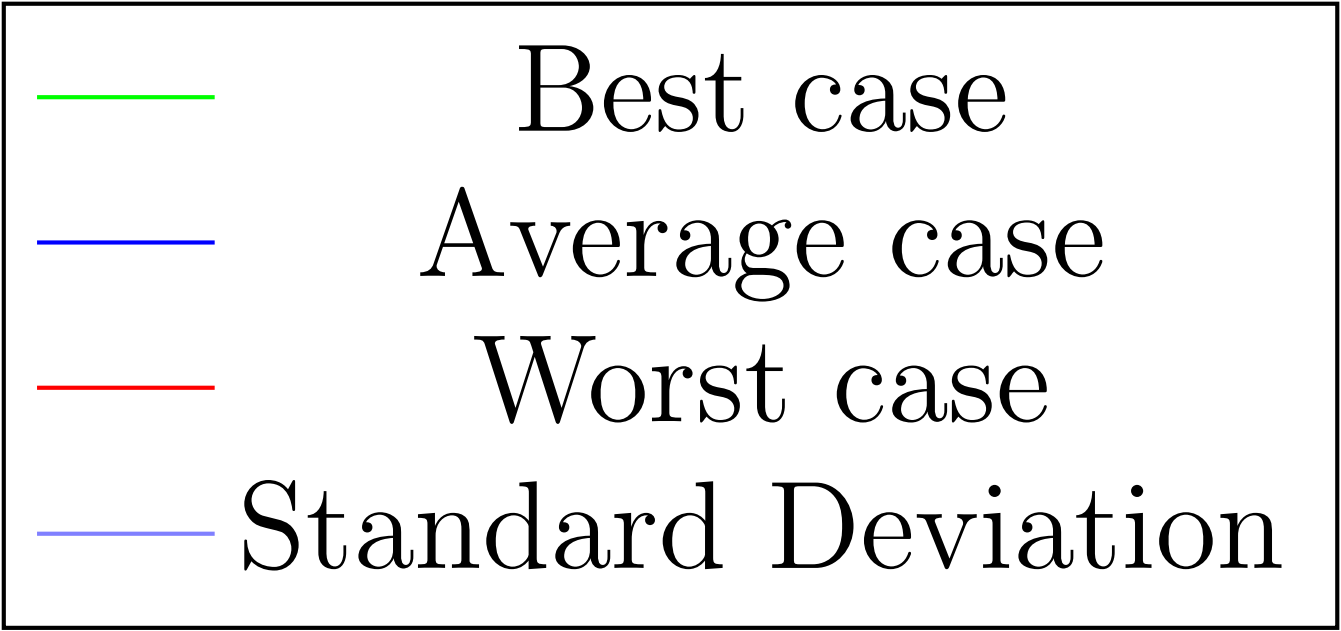
\includegraphics[scale=0.1]{chapters/res/generated_graph_legend.png}};
\end{tikzpicture}

\begin{figure}[H]
\vspace*{-1cm}
	\makebox[\linewidth][c]{%
	\begin{subfigure}[b]{0.7\textwidth}
		\centering
		\resizebox{0.9\linewidth}{!}{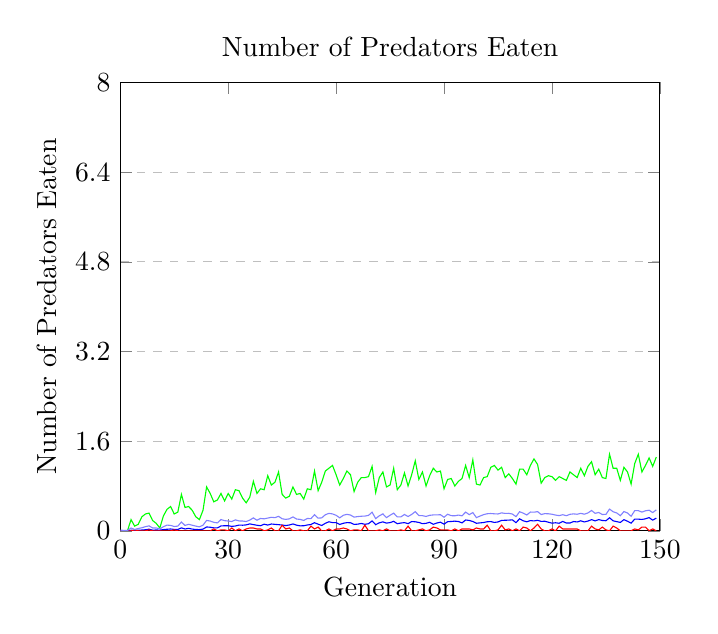
\begin{tikzpicture}
\begin{axis}[
	title={Number of Predators Eaten},
	xlabel={Generation},
	ylabel={Number of Predators Eaten},
	xmin=0, xmax=150,
	ymin=0, ymax=8,
	xtick={0.0,30.0,60.0,90.0,120.0,150.0},
	ytick={0.0,1.6,3.2,4.800000000000001,6.4,8.0},
	ymajorgrids=true,
	grid style=dashed,
]

\addplot[
	color=green,
	]
	coordinates {
	(0,0.0)(1,0.0)(2,0.0)(3,0.2)(4,0.08333333333333333)(5,0.11666666666666667)(6,0.25)(7,0.3)(8,0.31666666666666665)(9,0.18333333333333335)(10,0.13333333333333333)(11,0.05)(12,0.26666666666666666)(13,0.38333333333333336)(14,0.4333333333333333)(15,0.3)(16,0.33333333333333337)(17,0.65)(18,0.41666666666666674)(19,0.43333333333333335)(20,0.3666666666666667)(21,0.25)(22,0.2)(23,0.3666666666666667)(24,0.7833333333333333)(25,0.6666666666666666)(26,0.5166666666666666)(27,0.55)(28,0.6666666666666667)(29,0.5333333333333334)(30,0.6666666666666667)(31,0.5666666666666668)(32,0.7333333333333334)(33,0.7166666666666667)(34,0.5833333333333334)(35,0.5)(36,0.6000000000000001)(37,0.8833333333333334)(38,0.6666666666666666)(39,0.75)(40,0.7333333333333333)(41,0.9833333333333334)(42,0.8166666666666667)(43,0.8666666666666668)(44,1.0500000000000003)(45,0.65)(46,0.5833333333333334)(47,0.6166666666666667)(48,0.7833333333333333)(49,0.65)(50,0.6666666666666666)(51,0.5666666666666667)(52,0.75)(53,0.7333333333333333)(54,1.0666666666666667)(55,0.7166666666666667)(56,0.8666666666666668)(57,1.0666666666666667)(58,1.1166666666666667)(59,1.1666666666666667)(60,1.0)(61,0.8166666666666667)(62,0.9333333333333332)(63,1.0666666666666667)(64,0.9999999999999999)(65,0.7)(66,0.8666666666666667)(67,0.9500000000000002)(68,0.9500000000000001)(69,0.9666666666666668)(70,1.15)(71,0.6833333333333333)(72,0.95)(73,1.05)(74,0.7833333333333333)(75,0.8166666666666668)(76,1.1166666666666667)(77,0.7333333333333333)(78,0.8166666666666668)(79,1.0333333333333334)(80,0.7999999999999999)(81,1.0)(82,1.2500000000000002)(83,0.9166666666666666)(84,1.05)(85,0.8)(86,0.9833333333333334)(87,1.1166666666666667)(88,1.05)(89,1.0666666666666667)(90,0.75)(91,0.9166666666666666)(92,0.9333333333333333)(93,0.8000000000000002)(94,0.8833333333333334)(95,0.9333333333333332)(96,1.1666666666666667)(97,0.95)(98,1.2666666666666666)(99,0.8333333333333335)(100,0.8166666666666667)(101,0.9500000000000002)(102,0.9666666666666668)(103,1.1333333333333335)(104,1.166666666666667)(105,1.0833333333333335)(106,1.1333333333333333)(107,0.95)(108,1.0166666666666668)(109,0.9333333333333335)(110,0.8333333333333334)(111,1.0999999999999999)(112,1.0999999999999999)(113,1.0)(114,1.166666666666667)(115,1.2833333333333334)(116,1.1833333333333333)(117,0.8500000000000001)(118,0.9500000000000001)(119,0.9833333333333333)(120,0.9666666666666667)(121,0.9)(122,0.9666666666666668)(123,0.9333333333333335)(124,0.9000000000000001)(125,1.05)(126,1.0)(127,0.95)(128,1.1166666666666667)(129,0.9833333333333333)(130,1.1500000000000001)(131,1.2333333333333336)(132,1.0)(133,1.1)(134,0.9500000000000001)(135,0.9333333333333335)(136,1.3666666666666667)(137,1.1166666666666667)(138,1.1166666666666667)(139,0.9000000000000001)(140,1.1333333333333335)(141,1.0500000000000003)(142,0.8333333333333333)(143,1.2)(144,1.366666666666667)(145,1.0499999999999998)(146,1.1666666666666667)(147,1.2999999999999998)(148,1.1500000000000001)(149,1.3166666666666669)
	};
\addplot[
	color=blue,
	]
	coordinates {
	(0,0.0027777777777777775)(1,0.0013888888888888887)(2,0.0013888888888888887)(3,0.010416666666666668)(4,0.00625)(5,0.011805555555555555)(6,0.013888888888888886)(7,0.019444444444444445)(8,0.02916666666666666)(9,0.011805555555555554)(10,0.014583333333333332)(11,0.012499999999999997)(12,0.02222222222222222)(13,0.027777777777777773)(14,0.03263888888888889)(15,0.025)(16,0.02361111111111111)(17,0.05277777777777778)(18,0.03263888888888889)(19,0.04375)(20,0.031249999999999997)(21,0.022916666666666665)(22,0.022222222222222223)(23,0.029861111111111113)(24,0.06874999999999999)(25,0.06388888888888888)(26,0.05347222222222223)(27,0.051388888888888894)(28,0.08680555555555554)(29,0.09097222222222222)(30,0.09097222222222223)(31,0.07916666666666665)(32,0.08611111111111112)(33,0.10208333333333333)(34,0.09999999999999999)(35,0.10555555555555556)(36,0.12361111111111112)(37,0.11111111111111109)(38,0.09930555555555554)(39,0.09097222222222223)(40,0.11805555555555557)(41,0.10277777777777779)(42,0.12152777777777778)(43,0.11527777777777778)(44,0.10972222222222222)(45,0.10347222222222222)(46,0.09374999999999999)(47,0.10416666666666667)(48,0.1222222222222222)(49,0.10069444444444446)(50,0.08888888888888888)(51,0.09027777777777778)(52,0.10416666666666666)(53,0.11249999999999999)(54,0.14444444444444446)(55,0.11805555555555554)(56,0.0951388888888889)(57,0.13402777777777777)(58,0.1611111111111111)(59,0.14652777777777778)(60,0.14652777777777773)(61,0.1138888888888889)(62,0.13472222222222222)(63,0.14583333333333334)(64,0.14375000000000002)(65,0.11458333333333331)(66,0.11875)(67,0.13124999999999998)(68,0.1159722222222222)(69,0.12708333333333333)(70,0.1763888888888889)(71,0.10972222222222221)(72,0.1423611111111111)(73,0.1597222222222222)(74,0.1375)(75,0.14652777777777776)(76,0.16944444444444443)(77,0.12708333333333333)(78,0.13888888888888887)(79,0.14652777777777773)(80,0.12777777777777774)(81,0.16527777777777777)(82,0.1611111111111111)(83,0.14930555555555555)(84,0.12777777777777777)(85,0.13333333333333333)(86,0.15208333333333332)(87,0.11666666666666664)(88,0.1388888888888889)(89,0.15416666666666667)(90,0.11874999999999998)(91,0.1625)(92,0.16666666666666666)(93,0.17222222222222222)(94,0.16597222222222224)(95,0.14166666666666666)(96,0.1930555555555556)(97,0.18541666666666667)(98,0.1659722222222222)(99,0.13472222222222222)(100,0.14166666666666664)(101,0.14791666666666664)(102,0.16180555555555554)(103,0.1645833333333333)(104,0.14930555555555555)(105,0.15833333333333333)(106,0.18611111111111114)(107,0.1881944444444444)(108,0.1909722222222222)(109,0.19583333333333333)(110,0.1458333333333333)(111,0.21458333333333335)(112,0.17847222222222225)(113,0.1611111111111111)(114,0.18263888888888885)(115,0.17638888888888887)(116,0.1875)(117,0.16805555555555554)(118,0.1708333333333333)(119,0.15347222222222223)(120,0.13680555555555554)(121,0.14375)(122,0.13472222222222222)(123,0.16736111111111113)(124,0.13888888888888887)(125,0.1388888888888889)(126,0.16527777777777777)(127,0.15833333333333333)(128,0.17847222222222223)(129,0.15833333333333333)(130,0.17430555555555557)(131,0.1993055555555555)(132,0.17708333333333334)(133,0.19999999999999998)(134,0.18472222222222218)(135,0.17986111111111108)(136,0.23263888888888884)(137,0.1784722222222222)(138,0.1638888888888889)(139,0.15)(140,0.19930555555555554)(141,0.17083333333333336)(142,0.1375)(143,0.20833333333333331)(144,0.20833333333333331)(145,0.2027777777777778)(146,0.21388888888888888)(147,0.23541666666666666)(148,0.1909722222222222)(149,0.22638888888888886)
	};
\addplot[
	color=red,
	]
	coordinates {
	(0,0.0)(1,0.0)(2,0.0)(3,0.0)(4,0.016666666666666666)(5,0.0)(6,0.0)(7,0.0)(8,0.016666666666666666)(9,0.0)(10,0.0)(11,0.0)(12,0.0)(13,0.0)(14,0.0)(15,0.016666666666666666)(16,0.0)(17,0.0)(18,0.0)(19,0.0)(20,0.0)(21,0.0)(22,0.0)(23,0.0)(24,0.0)(25,0.0)(26,0.03333333333333333)(27,0.0)(28,0.016666666666666666)(29,0.016666666666666666)(30,0.0)(31,0.05)(32,0.0)(33,0.03333333333333333)(34,0.0)(35,0.03333333333333333)(36,0.05)(37,0.05)(38,0.03333333333333333)(39,0.03333333333333333)(40,0.0)(41,0.016666666666666666)(42,0.05)(43,0.0)(44,0.0)(45,0.1)(46,0.03333333333333333)(47,0.05)(48,0.0)(49,0.0)(50,0.016666666666666666)(51,0.0)(52,0.0)(53,0.08333333333333334)(54,0.03333333333333333)(55,0.06666666666666667)(56,0.0)(57,0.0)(58,0.03333333333333333)(59,0.0)(60,0.03333333333333333)(61,0.03333333333333333)(62,0.05)(63,0.03333333333333333)(64,0.0)(65,0.016666666666666666)(66,0.016666666666666666)(67,0.0)(68,0.1)(69,0.0)(70,0.0)(71,0.0)(72,0.016666666666666666)(73,0.0)(74,0.03333333333333333)(75,0.0)(76,0.0)(77,0.0)(78,0.016666666666666666)(79,0.0)(80,0.08333333333333333)(81,0.0)(82,0.0)(83,0.016666666666666666)(84,0.03333333333333333)(85,0.0)(86,0.016666666666666666)(87,0.06666666666666667)(88,0.05)(89,0.016666666666666666)(90,0.016666666666666666)(91,0.016666666666666666)(92,0.0)(93,0.03333333333333333)(94,0.0)(95,0.03333333333333333)(96,0.03333333333333333)(97,0.03333333333333333)(98,0.016666666666666666)(99,0.05)(100,0.03333333333333333)(101,0.03333333333333333)(102,0.1)(103,0.0)(104,0.0)(105,0.016666666666666666)(106,0.1)(107,0.016666666666666666)(108,0.03333333333333333)(109,0.0)(110,0.03333333333333333)(111,0.0)(112,0.06666666666666667)(113,0.05)(114,0.0)(115,0.05)(116,0.11666666666666667)(117,0.03333333333333333)(118,0.0)(119,0.0)(120,0.03333333333333333)(121,0.0)(122,0.08333333333333334)(123,0.03333333333333333)(124,0.03333333333333333)(125,0.03333333333333333)(126,0.03333333333333333)(127,0.03333333333333333)(128,0.0)(129,0.0)(130,0.0)(131,0.08333333333333334)(132,0.03333333333333333)(133,0.016666666666666666)(134,0.06666666666666667)(135,0.016666666666666666)(136,0.0)(137,0.08333333333333334)(138,0.05)(139,0.0)(140,0.0)(141,0.0)(142,0.0)(143,0.03333333333333333)(144,0.016666666666666666)(145,0.06666666666666667)(146,0.06666666666666667)(147,0.0)(148,0.03333333333333333)(149,0.0)
	};
\addplot[
	color=blue!50,
	]
	coordinates {
	(0,0.013321754231424218)(1,0.006660877115712111)(2,0.006660877115712111)(3,0.04995657836784082)(4,0.02462416810808586)(5,0.041714712917161424)(6,0.054776086736533204)(7,0.07400281405281414)(8,0.08890796547937019)(9,0.05076093250278195)(10,0.050340260506017455)(11,0.03493756482295231)(12,0.07340157477069524)(13,0.10160659562411234)(14,0.0967471195588641)(15,0.07752211412672846)(16,0.08384324732182037)(17,0.15694384396912922)(18,0.09529011233427392)(19,0.11603410156105053)(20,0.100267861430328)(21,0.08427225318868495)(22,0.07018169508420546)(23,0.10077201613448467)(24,0.18560012706790055)(25,0.17428340905864692)(26,0.15112630872184657)(27,0.141168525610981)(28,0.20133429843660738)(29,0.1811345193993133)(30,0.1748941500211222)(31,0.16498363310879754)(32,0.19593991614961265)(33,0.17635364551742774)(34,0.17487982891759307)(35,0.16525593881671272)(36,0.19196512690571463)(37,0.23052287962566761)(38,0.1889607737656392)(39,0.22060609492583494)(40,0.21351342399168433)(41,0.2273981531209474)(42,0.24121629967015934)(43,0.2349045046887506)(44,0.258442325399722)(45,0.21493663624424716)(46,0.20376359009757142)(47,0.21344909204960788)(48,0.24811102951958092)(49,0.2103238877627514)(50,0.2038208553145404)(51,0.1854738789478445)(52,0.22006802373976034)(53,0.21725136078204374)(54,0.2875201667126666)(55,0.22623762937080324)(56,0.23050677515137669)(57,0.28675413007961703)(58,0.311566049894099)(59,0.3017401676344359)(60,0.27699951462810235)(61,0.23168284733363256)(62,0.27708512773983296)(63,0.2942204488141478)(64,0.28136089090682814)(65,0.2442208497546257)(66,0.2543877768318327)(67,0.260208897746608)(68,0.2629816319576621)(69,0.2750320535869742)(70,0.33251932630243436)(71,0.2172413958051245)(72,0.26812139282597497)(73,0.3019337272407384)(74,0.23596127541107445)(75,0.27776910697717977)(76,0.3152794328834964)(77,0.2479913492161294)(78,0.2494532846163561)(79,0.29179818211535336)(80,0.25526410445178604)(81,0.292394363174823)(82,0.3422736388365272)(83,0.2727712479552301)(84,0.27079476560393734)(85,0.25623092678182136)(86,0.27664669395544494)(87,0.28360139722445316)(88,0.2840853730296988)(89,0.28751399940049743)(90,0.24219166298842468)(91,0.29577728618930715)(92,0.2702274272848864)(93,0.2684012606189619)(94,0.2807840892846732)(95,0.26803194803149466)(96,0.3338138154099765)(97,0.28888359085338494)(98,0.32546056607413804)(99,0.23583334908008913)(100,0.26299823452404714)(101,0.2886659058784379)(102,0.3049099739955437)(103,0.30861293310835236)(104,0.3035893342396425)(105,0.3005233774232091)(106,0.32019623083462023)(107,0.31037801880257554)(108,0.3125403172395045)(109,0.29923281641780003)(110,0.2528833926893325)(111,0.34079862557377605)(112,0.31593145712369164)(113,0.2825951416775331)(114,0.33491398440218995)(115,0.3325202023294936)(116,0.3425758923166698)(117,0.290782209785977)(118,0.306709234064417)(119,0.30397909153011515)(120,0.29586496496088777)(121,0.2810733843091308)(122,0.27109009836261205)(123,0.28706667694059224)(124,0.26985425977353733)(125,0.2944704427303834)(126,0.3023189765475024)(127,0.295695154883936)(128,0.3120590599204607)(129,0.29647856169513154)(130,0.31919946814267247)(131,0.3631865167585294)(132,0.312373143338114)(133,0.3267970287088765)(134,0.2912584883608067)(135,0.2935138057011127)(136,0.38792914347170704)(137,0.3405499192599511)(138,0.3194330281852589)(139,0.2697103534143904)(140,0.3437004679373083)(141,0.3178881213640553)(142,0.25915266685291255)(143,0.3601022173153716)(144,0.35982403300276183)(145,0.3338391417571146)(146,0.3577831796449167)(147,0.3672246312203614)(148,0.32554690762123023)(149,0.3737249150439296)
	};
\end{axis}
\end{tikzpicture}
}
		\caption{Some sample caption}
	\end{subfigure}%
	\begin{subfigure}[b]{0.7\textwidth}		
		\centering
		\resizebox{0.9\linewidth}{!}{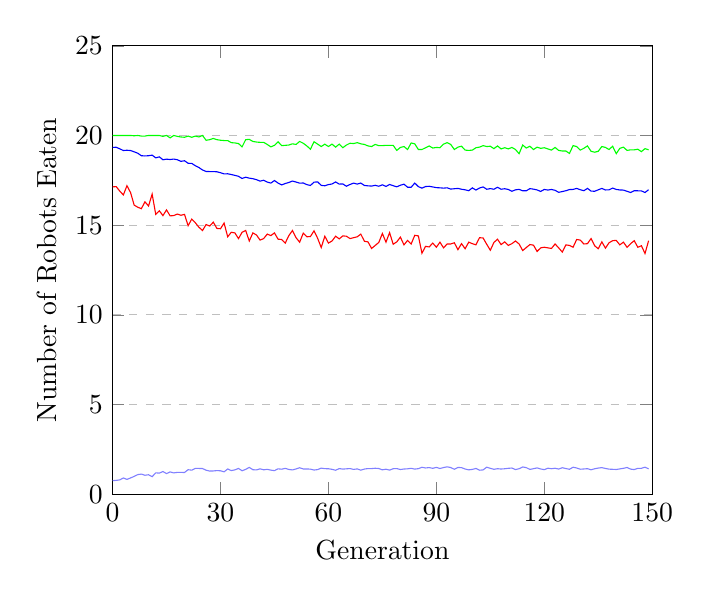
\begin{tikzpicture}
\begin{axis}[
	xlabel={Generation},
	ylabel={Number of Robots Eaten},
	xmin=0, xmax=150,
	ymin=0, ymax=25,
	xtick={0.0,30.0,60.0,90.0,120.0,150.0},
	ytick={0.0,5.0,10.0,15.0,20.0,25.0},
	ymajorgrids=true,
	grid style=dashed,
]

\addplot[
	color=green,
	]
	coordinates {
	(0,20.0)(1,20.0)(2,20.0)(3,20.0)(4,20.0)(5,20.0)(6,19.983333333333334)(7,20.0)(8,19.96666666666667)(9,19.96666666666667)(10,20.0)(11,20.0)(12,20.0)(13,20.0)(14,19.95)(15,20.0)(16,19.866666666666667)(17,20.0)(18,19.95)(19,19.916666666666664)(20,19.9)(21,19.96666666666667)(22,19.900000000000002)(23,19.96666666666667)(24,19.916666666666668)(25,20.0)(26,19.73333333333333)(27,19.76666666666667)(28,19.833333333333332)(29,19.766666666666666)(30,19.73333333333333)(31,19.71666666666667)(32,19.71666666666667)(33,19.599999999999998)(34,19.583333333333332)(35,19.549999999999997)(36,19.366666666666664)(37,19.766666666666666)(38,19.783333333333335)(39,19.666666666666668)(40,19.63333333333333)(41,19.616666666666667)(42,19.616666666666664)(43,19.499999999999996)(44,19.366666666666664)(45,19.450000000000003)(46,19.65)(47,19.433333333333334)(48,19.45)(49,19.466666666666665)(50,19.53333333333333)(51,19.5)(52,19.666666666666668)(53,19.566666666666666)(54,19.416666666666664)(55,19.233333333333334)(56,19.65)(57,19.516666666666666)(58,19.38333333333333)(59,19.516666666666666)(60,19.383333333333333)(61,19.516666666666662)(62,19.349999999999998)(63,19.516666666666666)(64,19.316666666666663)(65,19.466666666666665)(66,19.566666666666663)(67,19.549999999999997)(68,19.6)(69,19.53333333333333)(70,19.5)(71,19.416666666666668)(72,19.38333333333333)(73,19.499999999999996)(74,19.433333333333334)(75,19.43333333333333)(76,19.45)(77,19.449999999999996)(78,19.45)(79,19.166666666666664)(80,19.33333333333333)(81,19.38333333333333)(82,19.216666666666665)(83,19.58333333333333)(84,19.533333333333328)(85,19.21666666666666)(86,19.21666666666666)(87,19.316666666666666)(88,19.416666666666664)(89,19.3)(90,19.333333333333332)(91,19.316666666666666)(92,19.51666666666667)(93,19.599999999999998)(94,19.5)(95,19.216666666666665)(96,19.349999999999994)(97,19.400000000000002)(98,19.183333333333334)(99,19.166666666666668)(100,19.183333333333334)(101,19.316666666666666)(102,19.349999999999994)(103,19.43333333333333)(104,19.38333333333333)(105,19.399999999999995)(106,19.266666666666662)(107,19.416666666666664)(108,19.249999999999996)(109,19.316666666666666)(110,19.249999999999996)(111,19.333333333333332)(112,19.216666666666665)(113,18.98333333333333)(114,19.466666666666665)(115,19.299999999999997)(116,19.399999999999995)(117,19.21666666666667)(118,19.349999999999998)(119,19.283333333333335)(120,19.316666666666666)(121,19.25)(122,19.18333333333333)(123,19.333333333333336)(124,19.166666666666664)(125,19.133333333333333)(126,19.13333333333333)(127,18.999999999999996)(128,19.433333333333334)(129,19.383333333333336)(130,19.18333333333333)(131,19.28333333333333)(132,19.416666666666668)(133,19.116666666666664)(134,19.066666666666663)(135,19.116666666666667)(136,19.383333333333333)(137,19.333333333333332)(138,19.216666666666665)(139,19.4)(140,18.98333333333333)(141,19.28333333333333)(142,19.349999999999994)(143,19.166666666666664)(144,19.199999999999996)(145,19.200000000000003)(146,19.23333333333333)(147,19.099999999999998)(148,19.266666666666666)(149,19.199999999999996)
	};
\addplot[
	color=blue,
	]
	coordinates {
	(0,19.334722222222226)(1,19.343055555555555)(2,19.256944444444446)(3,19.160416666666666)(4,19.17638888888889)(5,19.160416666666666)(6,19.08888888888889)(7,19.009722222222226)(8,18.87152777777778)(9,18.858333333333334)(10,18.871527777777782)(11,18.903472222222224)(12,18.751388888888886)(13,18.808333333333334)(14,18.645833333333336)(15,18.679861111111112)(16,18.65972222222222)(17,18.68402777777778)(18,18.647222222222222)(19,18.55763888888889)(20,18.590277777777775)(21,18.450000000000003)(22,18.442361111111115)(23,18.31597222222222)(24,18.213194444444447)(25,18.076388888888893)(26,17.993055555555554)(27,17.9875)(28,17.986805555555556)(29,17.975694444444446)(30,17.92291666666667)(31,17.85763888888889)(32,17.86388888888889)(33,17.822222222222226)(34,17.774305555555557)(35,17.72361111111111)(36,17.602777777777778)(37,17.672916666666662)(38,17.62013888888889)(39,17.589583333333337)(40,17.536111111111115)(41,17.45347222222222)(42,17.50347222222222)(43,17.4)(44,17.34583333333333)(45,17.488194444444446)(46,17.34652777777778)(47,17.243750000000002)(48,17.320138888888888)(49,17.379166666666666)(50,17.457638888888887)(51,17.403472222222224)(52,17.34027777777778)(53,17.350694444444443)(54,17.258333333333333)(55,17.213194444444447)(56,17.396527777777777)(57,17.411805555555556)(58,17.215277777777775)(59,17.19513888888889)(60,17.260416666666668)(61,17.294444444444444)(62,17.40972222222222)(63,17.28888888888889)(64,17.297222222222228)(65,17.168055555555558)(66,17.266666666666666)(67,17.34444444444444)(68,17.28888888888889)(69,17.347222222222225)(70,17.213888888888885)(71,17.19166666666667)(72,17.177083333333332)(73,17.221527777777776)(74,17.16944444444444)(75,17.247916666666665)(76,17.158333333333335)(77,17.265972222222224)(78,17.19861111111111)(79,17.136805555555554)(80,17.224999999999998)(81,17.284722222222218)(82,17.11458333333333)(83,17.114583333333336)(84,17.346527777777776)(85,17.147916666666667)(86,17.062499999999996)(87,17.15277777777778)(88,17.166666666666668)(89,17.12986111111111)(90,17.090972222222224)(91,17.080555555555556)(92,17.063194444444445)(93,17.081944444444446)(94,17.009722222222223)(95,17.03055555555556)(96,17.047222222222224)(97,17.00208333333333)(98,16.96875)(99,16.919444444444448)(100,17.077083333333334)(101,16.95625)(102,17.07013888888889)(103,17.131249999999998)(104,16.999305555555555)(105,17.036805555555556)(106,17.002083333333335)(107,17.11111111111111)(108,17.002777777777776)(109,17.02986111111111)(110,16.989583333333336)(111,16.888888888888886)(112,16.969444444444445)(113,16.995138888888892)(114,16.915972222222223)(115,16.916666666666668)(116,17.036111111111108)(117,17.007638888888888)(118,16.963194444444447)(119,16.879166666666666)(120,16.990972222222222)(121,16.954861111111114)(122,16.989583333333332)(123,16.941666666666666)(124,16.830555555555556)(125,16.87291666666667)(126,16.919444444444448)(127,16.98402777777778)(128,16.990972222222222)(129,17.04791666666667)(130,16.975694444444443)(131,16.920138888888893)(132,17.048611111111114)(133,16.899305555555557)(134,16.88819444444444)(135,16.97013888888889)(136,17.047222222222224)(137,16.961805555555554)(138,16.96805555555556)(139,17.06736111111111)(140,16.990972222222222)(141,16.961805555555554)(142,16.95486111111111)(143,16.8875)(144,16.81944444444444)(145,16.918055555555558)(146,16.914583333333336)(147,16.909722222222225)(148,16.819444444444446)(149,16.976388888888884)
	};
\addplot[
	color=red,
	]
	coordinates {
	(0,17.133333333333336)(1,17.15)(2,16.900000000000002)(3,16.683333333333334)(4,17.2)(5,16.81666666666667)(6,16.116666666666664)(7,16.0)(8,15.916666666666668)(9,16.3)(10,16.066666666666666)(11,16.73333333333333)(12,15.600000000000001)(13,15.799999999999999)(14,15.533333333333333)(15,15.850000000000001)(16,15.516666666666666)(17,15.533333333333331)(18,15.616666666666665)(19,15.549999999999999)(20,15.599999999999998)(21,14.966666666666667)(22,15.333333333333332)(23,15.133333333333335)(24,14.883333333333335)(25,14.700000000000003)(26,15.033333333333333)(27,14.95)(28,15.166666666666668)(29,14.816666666666668)(30,14.799999999999999)(31,15.116666666666667)(32,14.350000000000001)(33,14.600000000000001)(34,14.566666666666668)(35,14.25)(36,14.6)(37,14.700000000000001)(38,14.116666666666667)(39,14.56666666666667)(40,14.450000000000001)(41,14.166666666666668)(42,14.25)(43,14.5)(44,14.416666666666668)(45,14.566666666666668)(46,14.216666666666667)(47,14.199999999999998)(48,14.000000000000002)(49,14.416666666666666)(50,14.7)(51,14.299999999999999)(52,14.049999999999999)(53,14.55)(54,14.349999999999998)(55,14.366666666666667)(56,14.683333333333334)(57,14.26666666666667)(58,13.75)(59,14.383333333333331)(60,14.0)(61,14.116666666666664)(62,14.383333333333331)(63,14.23333333333333)(64,14.4)(65,14.383333333333335)(66,14.250000000000002)(67,14.300000000000002)(68,14.350000000000003)(69,14.5)(70,14.1)(71,14.066666666666668)(72,13.699999999999996)(73,13.866666666666669)(74,14.033333333333335)(75,14.533333333333335)(76,14.05)(77,14.583333333333334)(78,13.933333333333332)(79,14.066666666666668)(80,14.333333333333332)(81,13.900000000000004)(82,14.15)(83,13.950000000000001)(84,14.433333333333334)(85,14.4)(86,13.433333333333332)(87,13.816666666666665)(88,13.783333333333335)(89,14.0)(90,13.766666666666667)(91,14.049999999999999)(92,13.733333333333333)(93,13.950000000000001)(94,13.950000000000001)(95,14.016666666666666)(96,13.633333333333333)(97,13.966666666666669)(98,13.683333333333332)(99,14.049999999999999)(100,13.966666666666665)(101,13.900000000000002)(102,14.3)(103,14.283333333333333)(104,13.933333333333334)(105,13.600000000000001)(106,14.033333333333333)(107,14.216666666666669)(108,13.91666666666667)(109,14.06666666666667)(110,13.866666666666667)(111,13.966666666666665)(112,14.116666666666667)(113,13.95)(114,13.583333333333334)(115,13.75)(116,13.916666666666668)(117,13.883333333333335)(118,13.533333333333333)(119,13.733333333333336)(120,13.76666666666667)(121,13.733333333333334)(122,13.7)(123,13.950000000000003)(124,13.733333333333333)(125,13.5)(126,13.9)(127,13.866666666666667)(128,13.766666666666664)(129,14.2)(130,14.166666666666666)(131,13.95)(132,13.966666666666667)(133,14.250000000000002)(134,13.849999999999998)(135,13.683333333333334)(136,14.066666666666668)(137,13.716666666666667)(138,14.016666666666666)(139,14.133333333333335)(140,14.149999999999999)(141,13.9)(142,14.049999999999997)(143,13.766666666666666)(144,13.966666666666667)(145,14.133333333333333)(146,13.766666666666667)(147,13.850000000000001)(148,13.416666666666668)(149,14.133333333333333)
	};
\addplot[
	color=blue!50,
	]
	coordinates {
	(0,0.7495221654824293)(1,0.7667849512222111)(2,0.7937800159652828)(3,0.9009319955456466)(4,0.821421066088009)(5,0.9033778184801008)(6,0.9885516545943156)(7,1.0877092135149327)(8,1.1185015019217932)(9,1.0530244041702717)(10,1.080212096519034)(11,0.9732174931705629)(12,1.1865590586974757)(13,1.172072868665637)(14,1.2597930436215803)(15,1.1458588788721191)(16,1.2379464941996747)(17,1.1843843030227519)(18,1.2132323105756961)(19,1.2103633566413428)(20,1.2077650916609217)(21,1.3621833907109868)(22,1.3370486755417135)(23,1.4323696938873278)(24,1.4326193779025012)(25,1.4263226218237772)(26,1.333554788982709)(27,1.286275589019169)(28,1.292836207572153)(29,1.31235276796664)(30,1.3025068678843843)(31,1.2424717474722389)(32,1.403392080946496)(33,1.3116699304373223)(34,1.352927045929469)(35,1.432432355507241)(36,1.3043591536561654)(37,1.3793611003412423)(38,1.4916848771428564)(39,1.3611092090934394)(40,1.3507727479126117)(41,1.4109570253852448)(42,1.3562349038319284)(43,1.3826043730614128)(44,1.3384977921634633)(45,1.309362110948463)(46,1.4115003175339216)(47,1.3901567308555127)(48,1.4371112704297024)(49,1.376802191993921)(50,1.3501863568339791)(51,1.4041083119568887)(52,1.4718548662993414)(53,1.4029641849239807)(54,1.4024661928870281)(55,1.394776365361264)(56,1.3428590476268158)(57,1.3686315116809038)(58,1.4496211414184197)(59,1.4199401445636624)(60,1.4155407347767308)(61,1.3833911892505895)(62,1.3317168205593122)(63,1.4248273845805426)(64,1.396111279625997)(65,1.4109374076247492)(66,1.4258927664603809)(67,1.3779786522511697)(68,1.4074023849447377)(69,1.3355616492778202)(70,1.3985905160673455)(71,1.4248360597926741)(72,1.4252259553877393)(73,1.442872785161671)(74,1.4267941374308009)(75,1.3544302907808747)(76,1.3905047521265983)(77,1.3389528748091777)(78,1.4172420542036246)(79,1.4256597795805186)(80,1.373830686675848)(81,1.3999529521057599)(82,1.4118277951106923)(83,1.4393074090931737)(84,1.3955719894174399)(85,1.4209755231072283)(86,1.4964772368244081)(87,1.45848783479382)(88,1.4801399434499836)(89,1.4386056971856005)(90,1.4913744024632718)(91,1.429537507805289)(92,1.4824075852702059)(93,1.5228209950593354)(94,1.4822887633918653)(95,1.3864413912518907)(96,1.4894401221761866)(97,1.4758309345921503)(98,1.400903185591091)(99,1.3530728964614878)(100,1.3784319372899336)(101,1.432322881528173)(102,1.3341627889334615)(103,1.350510878269627)(104,1.503157366027273)(105,1.4380328655013617)(106,1.3853154149130695)(107,1.4170254792376986)(108,1.400362969370859)(109,1.415009044805558)(110,1.439890159378201)(111,1.4556558110935705)(112,1.3681251322291648)(113,1.4177289512914264)(114,1.5171687335853408)(115,1.476415423390563)(116,1.3772700156948967)(117,1.4195875214213405)(118,1.4628750423706767)(119,1.4028219965369768)(120,1.3646152389686075)(121,1.444845843262628)(122,1.418242544370372)(123,1.4429242306745347)(124,1.3981740915593432)(125,1.4722678360929213)(126,1.427307290002399)(127,1.3854462592701688)(128,1.50119270631082)(129,1.4579553872261812)(130,1.389587227587588)(131,1.4031286351585264)(132,1.4200817659260205)(133,1.3569782945629658)(134,1.4138860664676742)(135,1.4538672893487978)(136,1.4767743553060562)(137,1.4322612666101897)(138,1.3930862565429252)(139,1.3842089109001219)(140,1.3736429590740122)(141,1.4066450237141703)(142,1.4395523619828012)(143,1.4850309889852185)(144,1.3945008720821126)(145,1.368513363542005)(146,1.4364385062503913)(147,1.4387771417617692)(148,1.5033535545825276)(149,1.4072605631818442)
	};
\end{axis}
\end{tikzpicture}
}
		\caption{Some sample caption}
	\end{subfigure}%
}
\\
\\
\\
	\makebox[\linewidth][c]{%
	\begin{subfigure}[b]{0.7\textwidth}
		\centering
		\resizebox{0.9\linewidth}{!}{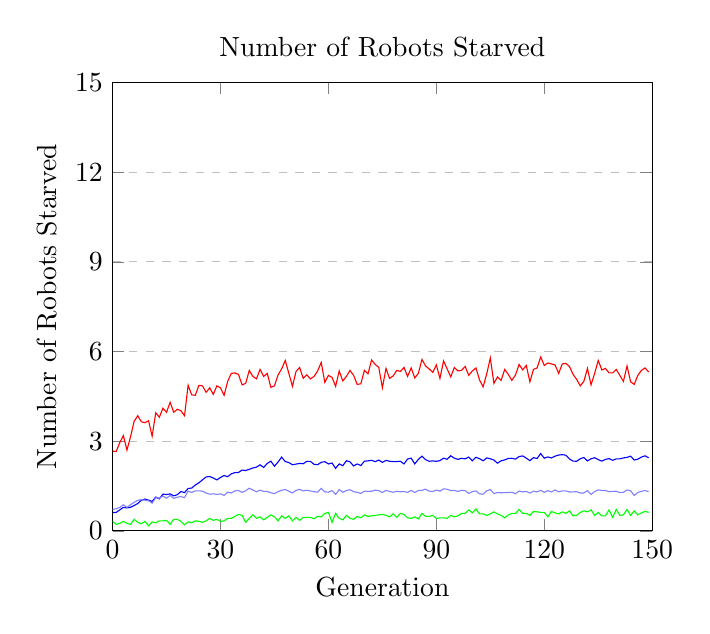
\begin{tikzpicture}
\begin{axis}[
	title={Number of Robots Starved},
	xlabel={Generation},
	ylabel={Number of Robots Starved},
	xmin=0, xmax=150,
	ymin=0, ymax=15,
	xtick={0.0,30.0,60.0,90.0,120.0,150.0},
	ytick={0.0,3.0,6.0,9.0,12.0,15.0},
	ymajorgrids=true,
	grid style=dashed,
]

\addplot[
	color=red,
	]
	coordinates {
	(0,2.6666666666666665)(1,2.65)(2,2.95)(3,3.183333333333333)(4,2.7)(5,3.15)(6,3.6666666666666665)(7,3.85)(8,3.6500000000000004)(9,3.6166666666666663)(10,3.6833333333333327)(11,3.1666666666666665)(12,3.9499999999999997)(13,3.8000000000000003)(14,4.1)(15,3.966666666666667)(16,4.3)(17,3.9666666666666663)(18,4.066666666666666)(19,4.016666666666667)(20,3.85)(21,4.866666666666667)(22,4.550000000000001)(23,4.533333333333334)(24,4.866666666666667)(25,4.8500000000000005)(26,4.633333333333333)(27,4.783333333333333)(28,4.566666666666666)(29,4.8500000000000005)(30,4.783333333333333)(31,4.533333333333333)(32,5.0)(33,5.2666666666666675)(34,5.283333333333334)(35,5.233333333333334)(36,4.883333333333334)(37,4.933333333333333)(38,5.366666666666666)(39,5.166666666666667)(40,5.083333333333334)(41,5.399999999999999)(42,5.166666666666667)(43,5.2666666666666675)(44,4.8)(45,4.8500000000000005)(46,5.216666666666667)(47,5.416666666666667)(48,5.700000000000002)(49,5.266666666666667)(50,4.833333333333333)(51,5.333333333333334)(52,5.466666666666667)(53,5.1000000000000005)(54,5.216666666666667)(55,5.083333333333334)(56,5.166666666666667)(57,5.35)(58,5.633333333333333)(59,4.966666666666667)(60,5.2)(61,5.133333333333334)(62,4.833333333333332)(63,5.3500000000000005)(64,5.016666666666667)(65,5.166666666666666)(66,5.366666666666666)(67,5.2)(68,4.9)(69,4.916666666666666)(70,5.366666666666668)(71,5.249999999999999)(72,5.716666666666666)(73,5.566666666666667)(74,5.466666666666667)(75,4.783333333333334)(76,5.433333333333333)(77,5.1000000000000005)(78,5.183333333333333)(79,5.366666666666666)(80,5.333333333333333)(81,5.466666666666667)(82,5.166666666666667)(83,5.45)(84,5.116666666666667)(85,5.2666666666666675)(86,5.733333333333333)(87,5.516666666666667)(88,5.416666666666667)(89,5.300000000000001)(90,5.55)(91,5.1000000000000005)(92,5.683333333333333)(93,5.416666666666667)(94,5.15)(95,5.466666666666667)(96,5.3500000000000005)(97,5.366666666666666)(98,5.500000000000001)(99,5.2)(100,5.35)(101,5.45)(102,5.05)(103,4.816666666666666)(104,5.25)(105,5.783333333333333)(106,4.933333333333334)(107,5.15)(108,5.033333333333333)(109,5.3999999999999995)(110,5.233333333333333)(111,5.033333333333333)(112,5.216666666666667)(113,5.566666666666666)(114,5.383333333333334)(115,5.533333333333333)(116,4.9833333333333325)(117,5.4)(118,5.45)(119,5.8166666666666655)(120,5.533333333333334)(121,5.616666666666667)(122,5.583333333333333)(123,5.55)(124,5.266666666666667)(125,5.583333333333333)(126,5.6000000000000005)(127,5.500000000000001)(128,5.233333333333334)(129,5.066666666666667)(130,4.85)(131,4.999999999999999)(132,5.433333333333333)(133,4.883333333333335)(134,5.266666666666667)(135,5.699999999999998)(136,5.383333333333334)(137,5.433333333333334)(138,5.283333333333333)(139,5.283333333333333)(140,5.4)(141,5.199999999999999)(142,5.000000000000001)(143,5.516666666666667)(144,4.983333333333333)(145,4.9)(146,5.2)(147,5.366666666666666)(148,5.45)(149,5.316666666666666)
	};
\addplot[
	color=blue,
	]
	coordinates {
	(0,0.6104166666666668)(1,0.6152777777777778)(2,0.698611111111111)(3,0.784027777777778)(4,0.765277777777778)(5,0.7881944444444444)(6,0.8465277777777778)(7,0.9131944444444444)(8,1.0229166666666665)(9,1.0638888888888889)(10,1.0256944444444442)(11,0.9840277777777776)(12,1.1298611111111112)(13,1.0694444444444444)(14,1.2256944444444444)(15,1.2152777777777775)(16,1.235416666666667)(17,1.1708333333333334)(18,1.2083333333333333)(19,1.3152777777777778)(20,1.2777777777777781)(21,1.4159722222222224)(22,1.43125)(23,1.5333333333333332)(24,1.6055555555555552)(25,1.7069444444444442)(26,1.8020833333333335)(27,1.8166666666666664)(28,1.7680555555555557)(29,1.7027777777777775)(30,1.7861111111111112)(31,1.8486111111111116)(32,1.8111111111111111)(33,1.9055555555555554)(34,1.9472222222222224)(35,1.9513888888888888)(36,2.033333333333333)(37,2.017361111111111)(38,2.0583333333333336)(39,2.102777777777778)(40,2.1305555555555555)(41,2.207638888888889)(42,2.11875)(43,2.2548611111111114)(44,2.329166666666666)(45,2.160416666666667)(46,2.302777777777778)(47,2.4659722222222227)(48,2.316666666666667)(49,2.2840277777777773)(50,2.209722222222222)(51,2.2326388888888884)(52,2.254166666666667)(53,2.24375)(54,2.325)(55,2.3236111111111115)(56,2.225694444444444)(57,2.2118055555555554)(58,2.2930555555555556)(59,2.3131944444444446)(60,2.236805555555556)(61,2.269444444444445)(62,2.089583333333333)(63,2.2381944444444444)(64,2.1798611111111117)(65,2.345138888888889)(66,2.3069444444444454)(67,2.16875)(68,2.238888888888888)(69,2.1826388888888886)(70,2.3312500000000003)(71,2.3395833333333336)(72,2.3590277777777784)(73,2.313888888888889)(74,2.3673611111111112)(75,2.2888888888888888)(76,2.3569444444444447)(77,2.3270833333333334)(78,2.3166666666666664)(79,2.3173611111111114)(80,2.3277777777777775)(81,2.2381944444444444)(82,2.4013888888888895)(83,2.4319444444444445)(84,2.238888888888889)(85,2.3909722222222225)(86,2.4958333333333336)(87,2.380555555555556)(88,2.327083333333334)(89,2.338888888888889)(90,2.324305555555556)(91,2.349305555555556)(92,2.4291666666666663)(93,2.3937500000000003)(94,2.510416666666667)(95,2.4305555555555554)(96,2.3895833333333334)(97,2.4256944444444444)(98,2.407638888888889)(99,2.467361111111111)(100,2.340972222222222)(101,2.4597222222222226)(102,2.4145833333333333)(103,2.341666666666667)(104,2.438888888888888)(105,2.4118055555555555)(106,2.3673611111111112)(107,2.2611111111111115)(108,2.3423611111111113)(109,2.3722222222222222)(110,2.4222222222222225)(111,2.427083333333334)(112,2.3986111111111112)(113,2.484722222222223)(114,2.505555555555556)(115,2.4312500000000004)(116,2.347222222222222)(117,2.4465277777777783)(118,2.4201388888888893)(119,2.584722222222222)(120,2.4298611111111112)(121,2.4722222222222223)(122,2.4361111111111113)(123,2.497916666666667)(124,2.5354166666666664)(125,2.5479166666666666)(126,2.5284722222222222)(127,2.404861111111112)(128,2.331944444444445)(129,2.3270833333333334)(130,2.4111111111111114)(131,2.4534722222222225)(132,2.338194444444445)(133,2.4104166666666664)(134,2.4458333333333337)(135,2.38125)(136,2.33125)(137,2.388888888888889)(138,2.417361111111111)(139,2.3590277777777775)(140,2.4069444444444446)(141,2.4090277777777778)(142,2.4381944444444446)(143,2.457638888888889)(144,2.497916666666666)(145,2.3673611111111112)(146,2.398611111111111)(147,2.466666666666667)(148,2.509027777777777)(149,2.44375)
	};
\addplot[
	color=green,
	]
	coordinates {
	(0,0.31666666666666665)(1,0.21666666666666665)(2,0.24999999999999997)(3,0.31666666666666665)(4,0.24999999999999997)(5,0.21666666666666665)(6,0.3833333333333333)(7,0.2833333333333333)(8,0.2333333333333333)(9,0.31666666666666665)(10,0.16666666666666666)(11,0.3)(12,0.26666666666666666)(13,0.3333333333333333)(14,0.3333333333333333)(15,0.35)(16,0.21666666666666665)(17,0.3833333333333333)(18,0.3833333333333333)(19,0.31666666666666665)(20,0.19999999999999998)(21,0.3)(22,0.26666666666666666)(23,0.3333333333333333)(24,0.31666666666666665)(25,0.2833333333333333)(26,0.3333333333333333)(27,0.41666666666666663)(28,0.35)(29,0.3833333333333333)(30,0.31666666666666665)(31,0.3333333333333333)(32,0.41666666666666663)(33,0.41666666666666663)(34,0.4833333333333333)(35,0.55)(36,0.5166666666666666)(37,0.2833333333333333)(38,0.41666666666666663)(39,0.5333333333333333)(40,0.41666666666666663)(41,0.4666666666666666)(42,0.36666666666666664)(43,0.44999999999999996)(44,0.5333333333333333)(45,0.4666666666666667)(46,0.3333333333333333)(47,0.5)(48,0.41666666666666663)(49,0.49999999999999994)(50,0.3333333333333333)(51,0.44999999999999996)(52,0.35)(53,0.44999999999999996)(54,0.44999999999999996)(55,0.44999999999999996)(56,0.39999999999999997)(57,0.4833333333333333)(58,0.4666666666666666)(59,0.5833333333333333)(60,0.6166666666666667)(61,0.2833333333333333)(62,0.5833333333333335)(63,0.41666666666666663)(64,0.36666666666666664)(65,0.5166666666666666)(66,0.41666666666666663)(67,0.3833333333333333)(68,0.4833333333333333)(69,0.4333333333333333)(70,0.5333333333333333)(71,0.4833333333333333)(72,0.49999999999999994)(73,0.5166666666666666)(74,0.5333333333333333)(75,0.5499999999999999)(76,0.5166666666666667)(77,0.4666666666666666)(78,0.5666666666666667)(79,0.44999999999999996)(80,0.5833333333333333)(81,0.5499999999999999)(82,0.4333333333333333)(83,0.41666666666666663)(84,0.4666666666666666)(85,0.39999999999999997)(86,0.5833333333333333)(87,0.4833333333333333)(88,0.4833333333333333)(89,0.5166666666666666)(90,0.41666666666666663)(91,0.4333333333333333)(92,0.4333333333333333)(93,0.41666666666666663)(94,0.5166666666666666)(95,0.4666666666666666)(96,0.5)(97,0.5833333333333335)(98,0.5833333333333334)(99,0.7)(100,0.6000000000000001)(101,0.7333333333333334)(102,0.5666666666666667)(103,0.5666666666666667)(104,0.5166666666666666)(105,0.5666666666666667)(106,0.6333333333333333)(107,0.5666666666666667)(108,0.5166666666666666)(109,0.4333333333333333)(110,0.5333333333333333)(111,0.5833333333333335)(112,0.5833333333333334)(113,0.7166666666666668)(114,0.5833333333333333)(115,0.5833333333333333)(116,0.5166666666666666)(117,0.6500000000000001)(118,0.6333333333333333)(119,0.6166666666666668)(120,0.6166666666666667)(121,0.4666666666666666)(122,0.6499999999999999)(123,0.6)(124,0.5666666666666667)(125,0.6333333333333333)(126,0.5833333333333333)(127,0.6666666666666667)(128,0.49999999999999994)(129,0.5166666666666666)(130,0.6166666666666666)(131,0.6666666666666666)(132,0.6333333333333333)(133,0.7000000000000002)(134,0.5166666666666667)(135,0.6166666666666667)(136,0.49999999999999994)(137,0.49999999999999994)(138,0.7)(139,0.45)(140,0.7166666666666666)(141,0.5166666666666666)(142,0.5333333333333334)(143,0.7166666666666668)(144,0.5166666666666667)(145,0.6666666666666667)(146,0.5333333333333333)(147,0.6)(148,0.65)(149,0.6166666666666667)
	};
\addplot[
	color=blue!50,
	]
	coordinates {
	(0,0.713161623888024)(1,0.7405015606242865)(2,0.7819253564877733)(3,0.8723607371449728)(4,0.7841301595134955)(5,0.8728015928897696)(6,0.953052632097735)(7,1.0199612174278232)(8,1.0420804993517523)(9,1.0222796199249384)(10,1.0070839119998525)(11,0.9246235039229337)(12,1.1070569581272676)(13,1.0925521154708617)(14,1.1624903223002732)(15,1.0917759526266515)(16,1.1856773654049817)(17,1.0871363477298965)(18,1.12480808320827)(19,1.1443987532040187)(20,1.11084343055975)(21,1.3270155736788916)(22,1.2834656265813822)(23,1.337662121482715)(24,1.3381732374390731)(25,1.3270232832570565)(26,1.2639830690927043)(27,1.2254607194898908)(28,1.2381053214053999)(29,1.2175842687406602)(30,1.2360878446601915)(31,1.1830520254543007)(32,1.2948210523548913)(33,1.2649311015836868)(34,1.336421777858519)(35,1.3479914075502182)(36,1.2871302893463945)(37,1.337557629016)(38,1.4271374648580106)(39,1.3628924752901934)(40,1.3044950082857705)(41,1.3603620997373091)(42,1.316414730820864)(43,1.3204888399932182)(44,1.2733282667710506)(45,1.2444270113009204)(46,1.3105825557350723)(47,1.3567273928680774)(48,1.3821804184838016)(49,1.3228880536133405)(50,1.2665555780783349)(51,1.3546682099848373)(52,1.3858459504582736)(53,1.3342581575407042)(54,1.357983325223933)(55,1.3335429525647595)(56,1.3086391315884098)(57,1.2917748339314072)(58,1.4219587806790843)(59,1.3037129324375627)(60,1.290605479376817)(61,1.3466313853861758)(62,1.2186336383040635)(63,1.3805844790410275)(64,1.2885152508784299)(65,1.3481487608785028)(66,1.374527882597602)(67,1.3087771377760256)(68,1.287822347183514)(69,1.248888617963421)(70,1.3294548586477166)(71,1.3185178444966288)(72,1.3256142854269775)(73,1.3599061511393482)(74,1.3421387834854497)(75,1.2835190273562596)(76,1.3510039738532438)(77,1.3188162292830492)(78,1.2892344807263973)(79,1.323417939126317)(80,1.3069162416583548)(81,1.3145145987682567)(82,1.2844648788830715)(83,1.352830141648675)(84,1.281351168994527)(85,1.3469710618723252)(86,1.352999479973355)(87,1.3942094677465784)(88,1.3283253695419528)(89,1.313869965002989)(90,1.3632938270008417)(91,1.325910294959868)(92,1.4050302717035508)(93,1.3909399113289962)(94,1.3464102934355326)(95,1.3493398577101285)(96,1.3171351931787447)(97,1.3557756150890636)(98,1.3449688209010366)(99,1.252538309255238)(100,1.3101945302963802)(101,1.3340553445887706)(102,1.2363492536605436)(103,1.2244270505874981)(104,1.3382745272304937)(105,1.3823931209428997)(106,1.244147356018067)(107,1.2810438290140636)(108,1.2723759589176842)(109,1.2790148315563936)(110,1.28240150353385)(111,1.289070858234679)(112,1.2415568849594845)(113,1.3302691426187627)(114,1.304465833718366)(115,1.3163821585732534)(116,1.2629395267908712)(117,1.3238359812644949)(118,1.301263148742386)(119,1.356066597766781)(120,1.2883787155893651)(121,1.3442440924131975)(122,1.3010439609213127)(123,1.365031739892029)(124,1.3050563975021297)(125,1.3343171810974497)(126,1.3339327428666283)(127,1.2969311706288806)(128,1.3024216212014035)(129,1.3104386498457024)(130,1.2632457537129205)(131,1.266827748274906)(132,1.3465649011709866)(133,1.214116583763829)(134,1.3146829760766328)(135,1.3682993864769921)(136,1.3507474365488252)(137,1.3483984551695007)(138,1.3107706708432896)(139,1.318182838577814)(140,1.3242677769396463)(141,1.2778017154534362)(142,1.289260575475016)(143,1.365699840622413)(144,1.3376908183956417)(145,1.180730498171941)(146,1.2816127339211778)(147,1.3219802983191828)(148,1.3463236016923459)(149,1.3127698393765261)
	};
\end{axis}
\end{tikzpicture}
}
		\caption{Some sample caption}
	\end{subfigure}%
	\begin{subfigure}[b]{0.7\textwidth}
		\centering
		\resizebox{0.9\linewidth}{!}{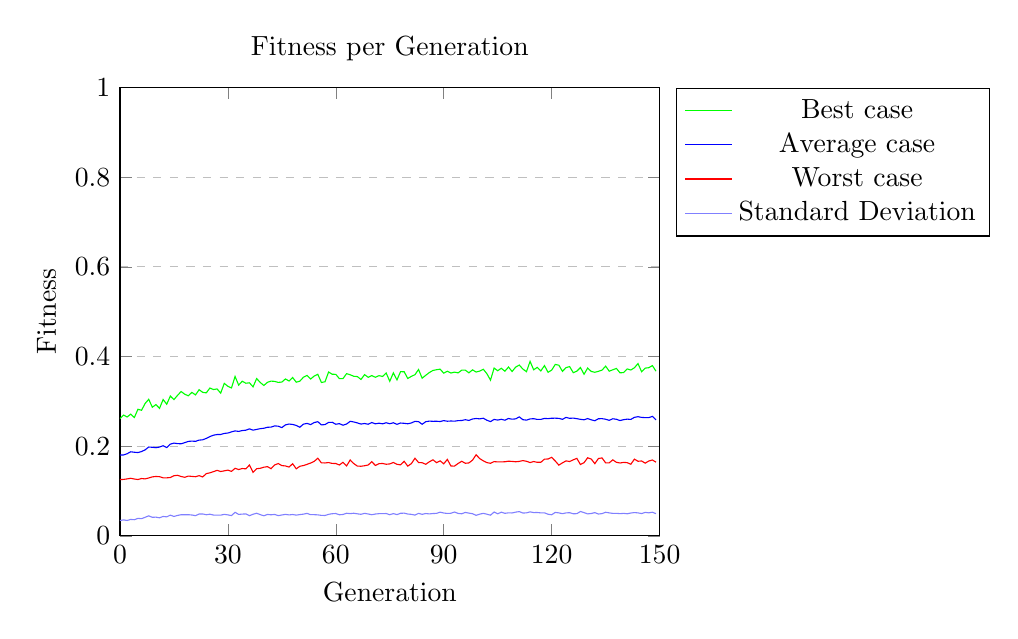
\begin{tikzpicture}
\begin{axis}[
	title={Fitness per Generation},
	xlabel={Generation},
	ylabel={Fitness},
	xmin=0, xmax=150,
	ymin=0, ymax=1,
	xtick={0.0,30.0,60.0,90.0,120.0,150.0},
	ytick={0.0,0.2,0.4,0.6000000000000001,0.8,1.0},
	legend pos=outer north east,
	ymajorgrids=true,
	grid style=dashed,
]

\addplot[
	color=green,
	]
	coordinates {
	(0,0.2616421666666667)(1,0.269403)(2,0.2652575833333333)(3,0.27150849999999993)(4,0.26399766666666663)(5,0.28241675000000005)(6,0.2801839166666666)(7,0.29536083333333335)(8,0.30473083333333334)(9,0.2869875)(10,0.2928463333333333)(11,0.2844886666666667)(12,0.30418491666666664)(13,0.29363825)(14,0.3118458333333334)(15,0.3040213333333333)(16,0.31333916666666667)(17,0.3220259999999999)(18,0.31602633333333335)(19,0.3125056666666666)(20,0.3201210833333333)(21,0.31434158333333334)(22,0.32611733333333337)(23,0.3202257500000001)(24,0.31899883333333323)(25,0.3299185833333333)(26,0.32638608333333335)(27,0.32781441666666666)(28,0.31843625000000003)(29,0.340128)(30,0.33366533333333337)(31,0.3299345)(32,0.3555909166666667)(33,0.33634100000000006)(34,0.34502108333333337)(35,0.34049241666666663)(36,0.34146541666666674)(37,0.33245133333333327)(38,0.35102041666666667)(39,0.34213883333333334)(40,0.33549874999999996)(41,0.34248208333333335)(42,0.3452323333333333)(43,0.3446361666666666)(44,0.34236824999999993)(45,0.3431215)(46,0.35005791666666675)(47,0.34552308333333326)(48,0.35334375)(49,0.3428407499999999)(50,0.3450749166666667)(51,0.35385991666666666)(52,0.35802408333333335)(53,0.3498753333333333)(54,0.35659725)(55,0.3604063333333334)(56,0.34213749999999993)(57,0.3437645833333333)(58,0.36556374999999997)(59,0.36056774999999996)(60,0.3603295000000001)(61,0.3506824166666667)(62,0.35091858333333326)(63,0.36188225)(64,0.35935433333333333)(65,0.3560165833333333)(66,0.3552922500000001)(67,0.34892033333333333)(68,0.359678)(69,0.3537624166666667)(70,0.3575265)(71,0.35376816666666666)(72,0.3574068333333333)(73,0.3556556666666667)(74,0.36325483333333336)(75,0.34480775)(76,0.3637045000000001)(77,0.3478945)(78,0.36635724999999997)(79,0.3660565)(80,0.35119624999999993)(81,0.35574325)(82,0.35958399999999996)(83,0.37111)(84,0.3517584166666666)(85,0.35819925)(86,0.36435016666666664)(87,0.3690029166666667)(88,0.37065675000000003)(89,0.3718781666666667)(90,0.3630023333333333)(91,0.36719850000000004)(92,0.3632859166666667)(93,0.36528333333333335)(94,0.36359958333333336)(95,0.3696236666666667)(96,0.3697404166666666)(97,0.36374624999999994)(98,0.37038583333333336)(99,0.36546233333333333)(100,0.367622)(101,0.37170583333333324)(102,0.3616952500000001)(103,0.34738558333333336)(104,0.37433508333333343)(105,0.3684105833333333)(106,0.3738935)(107,0.36730641666666664)(108,0.37661358333333333)(109,0.36662300000000003)(110,0.37651433333333334)(111,0.38104533333333335)(112,0.37207049999999997)(113,0.36627124999999994)(114,0.3892515833333333)(115,0.3704584999999999)(116,0.37602975)(117,0.36800108333333326)(118,0.37988550000000004)(119,0.3648296666666667)(120,0.36977800000000005)(121,0.38240341666666666)(122,0.38074474999999997)(123,0.36702175)(124,0.3753073333333334)(125,0.3776575)(126,0.36404283333333337)(127,0.36743925)(128,0.3754915833333333)(129,0.3605483333333333)(130,0.3742699166666667)(131,0.36680675)(132,0.36494375)(133,0.36705775)(134,0.36973333333333336)(135,0.3786206666666667)(136,0.36736025000000005)(137,0.37052416666666665)(138,0.3735159166666667)(139,0.3637445)(140,0.3642588333333333)(141,0.3724138333333333)(142,0.3700245833333334)(143,0.37497566666666665)(144,0.3843913333333333)(145,0.36624341666666677)(146,0.3742236666666667)(147,0.3751789166666666)(148,0.37981049999999994)(149,0.3673801666666667)
	};
	\addlegendentry{Best case}
\addplot[
	color=blue,
	]
	coordinates {
	(0,0.18053544791666667)(1,0.18047001736111112)(2,0.1832907673611111)(3,0.18759630902777777)(4,0.18657372569444447)(5,0.18584608333333333)(6,0.18808073958333332)(7,0.191941375)(8,0.1982048159722222)(9,0.19767581250000002)(10,0.19667909027777775)(11,0.19814942013888892)(12,0.20114278472222225)(13,0.19700895486111109)(14,0.2046636840277778)(15,0.20695594444444443)(16,0.20581769791666665)(17,0.20544595486111114)(18,0.20790242013888885)(19,0.2107393090277778)(20,0.2114579444444444)(21,0.21090147916666668)(22,0.2135970902777778)(23,0.21432137500000004)(24,0.217460375)(25,0.22153019791666664)(26,0.22461450347222223)(27,0.2260545138888889)(28,0.22624048611111117)(29,0.22851289236111114)(30,0.22942144791666672)(31,0.2320053333333333)(32,0.23416988194444446)(33,0.23307557638888893)(34,0.23494966319444444)(35,0.23576319444444443)(36,0.23872356597222222)(37,0.23580080555555558)(38,0.23754071875000002)(39,0.23913426041666666)(40,0.24009709722222228)(41,0.24225264583333334)(42,0.2426647326388889)(43,0.2453828923611111)(44,0.24468567708333333)(45,0.2415031666666667)(46,0.24758395486111104)(47,0.2494823090277778)(48,0.2485804201388889)(49,0.2464276840277778)(50,0.24244321527777782)(51,0.24924222569444446)(52,0.25087156597222227)(53,0.2482049236111111)(54,0.25283074305555553)(55,0.25470069791666666)(56,0.24760993750000002)(57,0.24827594791666663)(58,0.2530838125)(59,0.2533668090277778)(60,0.2490694756944445)(61,0.25032993750000004)(62,0.24692834027777782)(63,0.2495639826388889)(64,0.2555840729166666)(65,0.25409974305555555)(66,0.2519835486111111)(67,0.2494253923611111)(68,0.2506328541666667)(69,0.2490404375)(70,0.25286252777777773)(71,0.24996947222222227)(72,0.2513649201388889)(73,0.24998929166666667)(74,0.25232659375000005)(75,0.2502057951388889)(76,0.25231888888888887)(77,0.24886791319444443)(78,0.2517467569444445)(79,0.2511217152777778)(80,0.2500396423611111)(81,0.25189047569444445)(82,0.2555020833333334)(83,0.25478569444444443)(84,0.24896999652777774)(85,0.2546962847222223)(86,0.2560433125)(87,0.25553953124999995)(88,0.25570769791666664)(89,0.2550867881944444)(90,0.25711133680555553)(91,0.25574519444444443)(92,0.2562672604166666)(93,0.2558516875)(94,0.2571235347222222)(95,0.2573598715277778)(96,0.25919022222222227)(97,0.25753850000000006)(98,0.2607417395833333)(99,0.2618449236111111)(100,0.2610524722222223)(101,0.26242061805555555)(102,0.2579765069444444)(103,0.2548667673611111)(104,0.25982327777777775)(105,0.25828656597222227)(106,0.26009764583333334)(107,0.25804444444444447)(108,0.26182128472222227)(109,0.260297375)(110,0.2610393923611111)(111,0.2654688506944445)(112,0.25916913541666664)(113,0.25819959722222224)(114,0.26085788541666666)(115,0.26145201041666666)(116,0.25975414583333334)(117,0.25985242708333334)(118,0.26201575694444446)(119,0.26159204513888884)(120,0.2624260069444444)(121,0.26258177430555557)(122,0.2621073159722222)(123,0.2600359583333333)(124,0.26426944444444445)(125,0.2621826145833333)(126,0.2627993125)(127,0.2614083159722222)(128,0.2600229270833333)(129,0.25895810069444447)(130,0.26173341666666666)(131,0.25888363541666665)(132,0.25681273263888893)(133,0.26132322569444444)(134,0.2615036041666667)(135,0.2601779201388889)(136,0.25778075694444447)(137,0.26128697916666666)(138,0.26006636111111114)(139,0.25727417013888887)(140,0.2592614583333333)(141,0.2603828923611111)(142,0.25976334375000004)(143,0.26441786805555556)(144,0.26584540625)(145,0.2642967951388888)(146,0.26372665277777785)(147,0.2638707847222222)(148,0.26658189236111113)(149,0.2588132013888889)
	};
	\addlegendentry{Average case}
\addplot[
	color=red,
	]
	coordinates {
	(0,0.125617)(1,0.125969)(2,0.12707949999999996)(3,0.12850475)(4,0.12686925000000002)(5,0.12570699999999999)(6,0.12794183333333334)(7,0.12713025000000003)(8,0.12919333333333333)(9,0.13161283333333335)(10,0.13252850000000002)(11,0.13207375)(12,0.12948558333333332)(13,0.12947958333333331)(14,0.1301869166666667)(15,0.13409758333333333)(16,0.13518999999999998)(17,0.13245208333333333)(18,0.13074525)(19,0.1334108333333333)(20,0.13267616666666668)(21,0.13196574999999997)(22,0.13436441666666665)(23,0.13149125)(24,0.13886291666666664)(25,0.1406755)(26,0.14329816666666664)(27,0.14617808333333332)(28,0.14362624999999998)(29,0.14506066666666664)(30,0.14672633333333332)(31,0.1439190833333333)(32,0.1507085833333333)(33,0.14795125)(34,0.15027916666666663)(35,0.14951774999999998)(36,0.15810025)(37,0.14163858333333335)(38,0.14983033333333332)(39,0.1507508333333333)(40,0.15321316666666668)(41,0.15443791666666665)(42,0.14991600000000002)(43,0.15821783333333334)(44,0.16133341666666667)(45,0.15674283333333333)(46,0.1560913333333333)(47,0.15347641666666667)(48,0.1610348333333333)(49,0.14964341666666667)(50,0.15527249999999998)(51,0.1569214166666667)(52,0.15957241666666663)(53,0.16246399999999997)(54,0.16616666666666663)(55,0.17325791666666665)(56,0.16285391666666665)(57,0.16268508333333334)(58,0.16356208333333333)(59,0.16164908333333328)(60,0.16145199999999998)(61,0.15809399999999998)(62,0.16417199999999998)(63,0.15614424999999998)(64,0.16932008333333332)(65,0.1612545833333333)(66,0.1556509166666667)(67,0.15535158333333332)(68,0.1564499166666667)(69,0.15813983333333334)(70,0.16547066666666665)(71,0.15713691666666668)(72,0.16104516666666668)(73,0.1615514166666667)(74,0.15974916666666666)(75,0.160519)(76,0.16369325)(77,0.15973383333333335)(78,0.15842199999999998)(79,0.16630541666666665)(80,0.15564424999999998)(81,0.16119475)(82,0.17322649999999998)(83,0.16366816666666664)(84,0.16318850000000001)(85,0.15969675000000003)(86,0.16528458333333332)(87,0.16973900000000003)(88,0.163432)(89,0.16728858333333335)(90,0.16081916666666665)(91,0.17064091666666664)(92,0.1558496666666667)(93,0.15568691666666665)(94,0.16162441666666666)(95,0.16642208333333333)(96,0.16200075000000003)(97,0.16271233333333335)(98,0.16898241666666666)(99,0.18091941666666667)(100,0.17244375)(101,0.16736891666666667)(102,0.16343483333333333)(103,0.16192958333333338)(104,0.16571675)(105,0.16497133333333333)(106,0.1651355833333333)(107,0.16530541666666665)(108,0.16662616666666666)(109,0.16613999999999998)(110,0.16531791666666665)(111,0.16618025)(112,0.1679461666666667)(113,0.1664034166666667)(114,0.16357608333333334)(115,0.16582891666666666)(116,0.16413033333333332)(117,0.16427200000000003)(118,0.17116166666666663)(119,0.17154908333333338)(120,0.17518199999999998)(121,0.1670185833333333)(122,0.15786941666666665)(123,0.16291575)(124,0.1672995)(125,0.16586675000000003)(126,0.16969583333333332)(127,0.17288125)(128,0.15917433333333333)(129,0.16323233333333337)(130,0.1742105833333333)(131,0.1714605)(132,0.16114858333333337)(133,0.17261633333333334)(134,0.17391466666666666)(135,0.16288525)(136,0.16296666666666668)(137,0.16959575)(138,0.16410241666666667)(139,0.16263041666666667)(140,0.16395583333333333)(141,0.16335883333333334)(142,0.15974408333333331)(143,0.17113233333333333)(144,0.16644616666666667)(145,0.16709508333333334)(146,0.16222483333333332)(147,0.16697808333333333)(148,0.16930650000000003)(149,0.16436275000000003)
	};
	\addlegendentry{Worst case}
\addplot[
	color=blue!50,
	]
	coordinates {
	(0,0.03419160795402388)(1,0.03567270238489303)(2,0.03434451880034822)(3,0.036733849469053226)(4,0.03609770070467806)(5,0.0390362070825104)(6,0.038399288580897)(7,0.041473901334903716)(8,0.044706598499347064)(9,0.041442500888810935)(10,0.041819643301164486)(11,0.04027844351502153)(12,0.04344797170263369)(13,0.04239791959224113)(14,0.04636190466810991)(15,0.04338434052142545)(16,0.045548633946717695)(17,0.04722773365312542)(18,0.047030517946691795)(19,0.047243031879781336)(20,0.04660070542724015)(21,0.04509082221694779)(22,0.04875687303765856)(23,0.048945861814343634)(24,0.047158508099014666)(25,0.048387517514852235)(26,0.04648303433434054)(27,0.04623506052151194)(28,0.04628171771103422)(29,0.048050327430874104)(30,0.04688665019751587)(31,0.045303123646178965)(32,0.05262865864449882)(33,0.0479216849024418)(34,0.04859672065685812)(35,0.04900314415598731)(36,0.04502254697392385)(37,0.04827762102301221)(38,0.050501086586252984)(39,0.04746022778996142)(40,0.04487360623085305)(41,0.047817454811422376)(42,0.047050196956823075)(43,0.04783597134245706)(44,0.04521614441770994)(45,0.04659346494916556)(46,0.04797923988035963)(47,0.04676990375560612)(48,0.04763352180947531)(49,0.04631254667705463)(50,0.04748466112937285)(51,0.04851790792652637)(52,0.050169763792762646)(53,0.047345445799515974)(54,0.04733459608526517)(55,0.04688172927113893)(56,0.04572654716144692)(57,0.04551913271475561)(58,0.0480763811594364)(59,0.049425731667994556)(60,0.04990828351889687)(61,0.04708893854144226)(62,0.04776965168200148)(63,0.05046078012183634)(64,0.0497000150803483)(65,0.05050406880854063)(66,0.0491951371279147)(67,0.04813493474468012)(68,0.0503008493327201)(69,0.048853896059795864)(70,0.04720564604217493)(71,0.048752427970656737)(72,0.049600815808991144)(73,0.04955003596600054)(74,0.04990698637682603)(75,0.04726123807310031)(76,0.04975864938358559)(77,0.047433134690678946)(78,0.05042586704071486)(79,0.050723767758254504)(80,0.04875540783638532)(81,0.04802202044730743)(82,0.0463201101577072)(83,0.05025516509211207)(84,0.04809999380351773)(85,0.04987584576725819)(86,0.049019285504853044)(87,0.04987669598567431)(88,0.05020061373368318)(89,0.052871547864740916)(90,0.05100704548623868)(91,0.050050347331449266)(92,0.050447466649044356)(93,0.053197985633739814)(94,0.05010321485491176)(95,0.04931752044498829)(96,0.05239742538320529)(97,0.05075836302065315)(98,0.04946560256860545)(99,0.04588971974236326)(100,0.04849785231928734)(101,0.050322722258056944)(102,0.04836043093722586)(103,0.046171491494429624)(104,0.05321847527255677)(105,0.049213520599329964)(106,0.052907585383391305)(107,0.050340249680405576)(108,0.051457054497914934)(109,0.05113903885533)(110,0.05297854841508275)(111,0.05419913547896486)(112,0.05097168190032767)(113,0.05132699153054996)(114,0.05359285067580919)(115,0.05200655179104727)(116,0.052107116445220564)(117,0.051345752144849585)(118,0.05146785289920768)(119,0.048277024103596036)(120,0.047165398312625326)(121,0.05240991342376058)(122,0.05133069307266336)(123,0.04955076878967928)(124,0.051274980901690755)(125,0.05175389621950917)(126,0.049433084609259936)(127,0.04953492430626131)(128,0.05443098971771542)(129,0.051943722953140654)(130,0.049052129207906955)(131,0.04993529026432662)(132,0.05192155694452387)(133,0.04876617916351529)(134,0.049698217718238166)(135,0.052651676459720534)(136,0.05131516079685461)(137,0.05019643354920676)(138,0.050312079947177894)(139,0.04957127944666699)(140,0.05028021259234388)(141,0.04936691330663706)(142,0.05099328491045777)(143,0.05199718132118099)(144,0.05133265261344817)(145,0.04976457435682266)(146,0.052482324520393926)(147,0.05139146568876854)(148,0.05280954659998762)(149,0.04956871651010093)
	};
	\addlegendentry{Standard Deviation}
\end{axis}
\end{tikzpicture}
}
		\caption{Some sample caption}
	\end{subfigure}%
}
\caption{Figure shows results from a 3 connection port simulation (p.1)}
\end{figure}

\newpage
\vspace*{-2.0cm}
\textbf{\Huge Results - 3 ports (2)}
\vspace{1.5cm}
\begin{tikzpicture}[remember picture,overlay]
   \node[anchor=south east,inner sep=20pt] at (current page.south east)
              {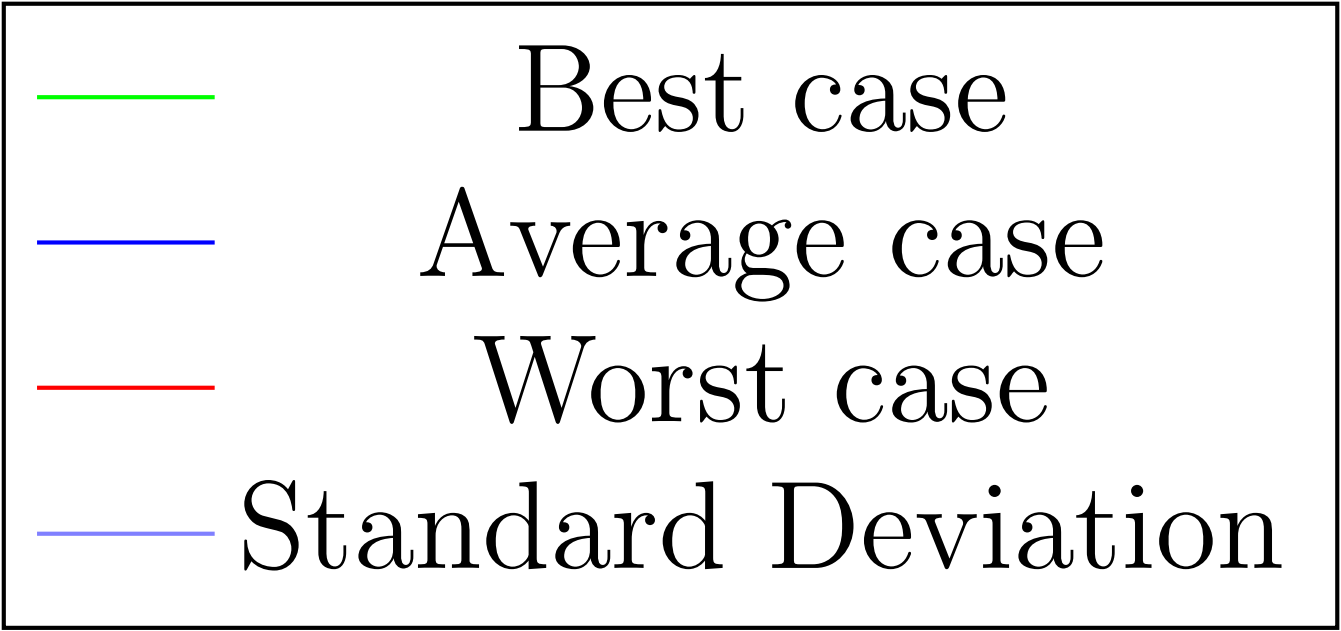
\includegraphics[scale=0.1]{chapters/res/generated_graph_legend.png}};
\end{tikzpicture}

\begin{figure}[H]
\vspace*{-1cm}
	\makebox[\linewidth][c]{%
	\begin{subfigure}[b]{0.7\textwidth}
		\centering
		\resizebox{0.9\linewidth}{!}{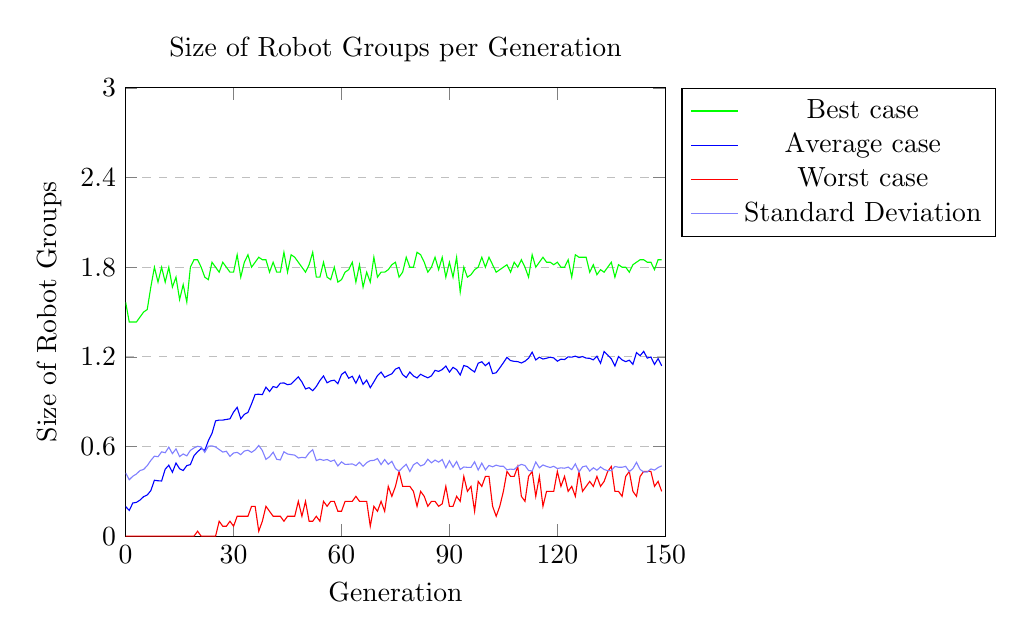
\begin{tikzpicture}
\begin{axis}[
	title={Size of Robot Groups per Generation},
	xlabel={Generation},
	ylabel={Size of Robot Groups},
	xmin=0, xmax=150,
	ymin=0, ymax=3,
	xtick={0.0,30.0,60.0,90.0,120.0,150.0},
	ytick={0.0,0.6,1.2,1.7999999999999998,2.4,3.0},
	legend pos=outer north east,
	ymajorgrids=true,
	grid style=dashed,
]

\addplot[
	color=green,
	]
	coordinates {
	(0,1.5666666666666669)(1,1.4333333333333333)(2,1.4333333333333333)(3,1.4333333333333336)(4,1.4666666666666668)(5,1.5000000000000002)(6,1.5166666666666668)(7,1.666666666666667)(8,1.8000000000000003)(9,1.7000000000000002)(10,1.8000000000000005)(11,1.7000000000000002)(12,1.8000000000000005)(13,1.666666666666667)(14,1.7333333333333336)(15,1.5833333333333337)(16,1.6833333333333336)(17,1.5666666666666669)(18,1.8000000000000005)(19,1.8500000000000005)(20,1.8500000000000005)(21,1.8000000000000007)(22,1.7333333333333336)(23,1.716666666666667)(24,1.8333333333333337)(25,1.8000000000000005)(26,1.766666666666667)(27,1.833333333333334)(28,1.8000000000000005)(29,1.7666666666666673)(30,1.766666666666667)(31,1.883333333333334)(32,1.7333333333333338)(33,1.833333333333334)(34,1.883333333333334)(35,1.8000000000000005)(36,1.833333333333334)(37,1.8666666666666674)(38,1.8500000000000008)(39,1.8500000000000005)(40,1.766666666666667)(41,1.833333333333334)(42,1.766666666666667)(43,1.766666666666667)(44,1.9000000000000006)(45,1.766666666666667)(46,1.883333333333334)(47,1.8666666666666671)(48,1.833333333333334)(49,1.8000000000000005)(50,1.766666666666667)(51,1.8166666666666673)(52,1.9000000000000008)(53,1.7333333333333336)(54,1.7333333333333338)(55,1.833333333333334)(56,1.7333333333333336)(57,1.7166666666666668)(58,1.8000000000000005)(59,1.7000000000000002)(60,1.716666666666667)(61,1.766666666666667)(62,1.7833333333333337)(63,1.833333333333334)(64,1.7000000000000004)(65,1.8166666666666673)(66,1.666666666666667)(67,1.766666666666667)(68,1.7000000000000004)(69,1.8666666666666674)(70,1.7333333333333338)(71,1.7666666666666673)(72,1.7666666666666673)(73,1.7833333333333339)(74,1.816666666666667)(75,1.833333333333334)(76,1.7333333333333336)(77,1.766666666666667)(78,1.8666666666666674)(79,1.8000000000000005)(80,1.8000000000000005)(81,1.9000000000000004)(82,1.883333333333334)(83,1.833333333333334)(84,1.766666666666667)(85,1.8000000000000005)(86,1.8666666666666674)(87,1.7833333333333339)(88,1.8666666666666674)(89,1.7333333333333338)(90,1.833333333333334)(91,1.7333333333333336)(92,1.8666666666666674)(93,1.6333333333333337)(94,1.8000000000000005)(95,1.7333333333333338)(96,1.7500000000000004)(97,1.7833333333333339)(98,1.8000000000000005)(99,1.8666666666666674)(100,1.8000000000000005)(101,1.8666666666666674)(102,1.8166666666666673)(103,1.766666666666667)(104,1.7833333333333339)(105,1.8000000000000005)(106,1.816666666666667)(107,1.766666666666667)(108,1.833333333333334)(109,1.8000000000000005)(110,1.8500000000000008)(111,1.8000000000000005)(112,1.7333333333333338)(113,1.883333333333334)(114,1.8000000000000005)(115,1.833333333333334)(116,1.8666666666666674)(117,1.833333333333334)(118,1.833333333333334)(119,1.8166666666666673)(120,1.833333333333334)(121,1.8000000000000005)(122,1.8000000000000005)(123,1.8500000000000008)(124,1.7333333333333338)(125,1.883333333333334)(126,1.8666666666666674)(127,1.8666666666666674)(128,1.8666666666666674)(129,1.7666666666666673)(130,1.816666666666667)(131,1.7500000000000002)(132,1.7833333333333337)(133,1.7666666666666673)(134,1.8000000000000005)(135,1.833333333333334)(136,1.7333333333333338)(137,1.816666666666667)(138,1.8000000000000005)(139,1.8000000000000005)(140,1.766666666666667)(141,1.816666666666667)(142,1.833333333333334)(143,1.8500000000000008)(144,1.8500000000000005)(145,1.8333333333333337)(146,1.833333333333334)(147,1.7833333333333337)(148,1.8500000000000005)(149,1.8500000000000008)
	};
	\addlegendentry{Best case}
\addplot[
	color=blue,
	]
	coordinates {
	(0,0.19861111111111107)(1,0.17222222222222222)(2,0.2222222222222222)(3,0.2263888888888889)(4,0.2416666666666666)(5,0.26458333333333334)(6,0.27569444444444446)(7,0.30486111111111114)(8,0.3743055555555555)(9,0.3708333333333333)(10,0.3694444444444444)(11,0.448611111111111)(12,0.47500000000000003)(13,0.42777777777777776)(14,0.4895833333333333)(15,0.4513888888888889)(16,0.43958333333333327)(17,0.4722222222222222)(18,0.4791666666666665)(19,0.5381944444444442)(20,0.5652777777777778)(21,0.586111111111111)(22,0.5743055555555554)(23,0.6388888888888888)(24,0.6875)(25,0.7715277777777777)(26,0.7770833333333332)(27,0.7770833333333331)(28,0.7812499999999998)(29,0.7854166666666667)(30,0.8305555555555554)(31,0.8624999999999999)(32,0.7854166666666665)(33,0.8152777777777778)(34,0.828472222222222)(35,0.8854166666666666)(36,0.9486111111111111)(37,0.9500000000000002)(38,0.9472222222222221)(39,0.9972222222222221)(40,0.9680555555555554)(41,1.0013888888888884)(42,0.9944444444444441)(43,1.023611111111111)(44,1.0256944444444445)(45,1.0138888888888888)(46,1.0180555555555553)(47,1.0423611111111113)(48,1.0659722222222223)(49,1.0319444444444443)(50,0.9854166666666664)(51,0.99375)(52,0.973611111111111)(53,1.0013888888888889)(54,1.0416666666666663)(55,1.0722222222222222)(56,1.0263888888888888)(57,1.0395833333333335)(58,1.0437500000000002)(59,1.0208333333333333)(60,1.0819444444444444)(61,1.1)(62,1.0569444444444442)(63,1.070138888888889)(64,1.023611111111111)(65,1.0743055555555554)(66,1.0159722222222223)(67,1.0444444444444443)(68,0.9937499999999999)(69,1.0326388888888889)(70,1.0743055555555556)(71,1.0986111111111112)(72,1.0631944444444443)(73,1.0756944444444447)(74,1.0868055555555554)(75,1.1180555555555556)(76,1.1291666666666664)(77,1.0812499999999998)(78,1.0618055555555554)(79,1.0986111111111112)(80,1.0722222222222222)(81,1.0590277777777777)(82,1.0833333333333333)(83,1.0708333333333333)(84,1.059722222222222)(85,1.0729166666666667)(86,1.1097222222222223)(87,1.102777777777778)(88,1.1152777777777776)(89,1.1388888888888888)(90,1.0979166666666667)(91,1.129861111111111)(92,1.114583333333333)(93,1.0784722222222223)(94,1.1423611111111112)(95,1.1347222222222224)(96,1.1152777777777778)(97,1.0986111111111112)(98,1.1576388888888889)(99,1.1673611111111108)(100,1.1409722222222223)(101,1.1625)(102,1.0881944444444445)(103,1.0937499999999998)(104,1.1263888888888889)(105,1.1604166666666667)(106,1.1965277777777776)(107,1.175)(108,1.1701388888888888)(109,1.1680555555555556)(110,1.1590277777777775)(111,1.1708333333333334)(112,1.190972222222222)(113,1.23125)(114,1.1791666666666667)(115,1.197916666666667)(116,1.1854166666666668)(117,1.1909722222222219)(118,1.1979166666666665)(119,1.1930555555555555)(120,1.1708333333333332)(121,1.1847222222222222)(122,1.1819444444444442)(123,1.2000000000000002)(124,1.1979166666666665)(125,1.2048611111111112)(126,1.1951388888888888)(127,1.2020833333333334)(128,1.1916666666666664)(129,1.1902777777777778)(130,1.179861111111111)(131,1.2048611111111112)(132,1.1569444444444443)(133,1.2361111111111112)(134,1.2125000000000001)(135,1.186805555555556)(136,1.1388888888888888)(137,1.2020833333333334)(138,1.1798611111111112)(139,1.1680555555555554)(140,1.1777777777777778)(141,1.15)(142,1.2284722222222222)(143,1.207638888888889)(144,1.2368055555555557)(145,1.1916666666666667)(146,1.1993055555555556)(147,1.1493055555555556)(148,1.1881944444444443)(149,1.140277777777778)
	};
	\addlegendentry{Average case}
\addplot[
	color=red,
	]
	coordinates {
	(0,0.0)(1,0.0)(2,0.0)(3,0.0)(4,0.0)(5,0.0)(6,0.0)(7,0.0)(8,0.0)(9,0.0)(10,0.0)(11,0.0)(12,0.0)(13,0.0)(14,0.0)(15,0.0)(16,0.0)(17,0.0)(18,0.0)(19,0.0)(20,0.03333333333333333)(21,0.0)(22,0.0)(23,0.0)(24,0.0)(25,0.0)(26,0.1)(27,0.06666666666666667)(28,0.06666666666666667)(29,0.1)(30,0.06666666666666667)(31,0.13333333333333333)(32,0.13333333333333333)(33,0.13333333333333333)(34,0.13333333333333333)(35,0.2)(36,0.2)(37,0.03333333333333333)(38,0.1)(39,0.19999999999999998)(40,0.16666666666666666)(41,0.13333333333333333)(42,0.13333333333333333)(43,0.13333333333333333)(44,0.1)(45,0.13333333333333333)(46,0.13333333333333333)(47,0.13333333333333333)(48,0.2333333333333333)(49,0.13333333333333333)(50,0.23333333333333334)(51,0.1)(52,0.1)(53,0.13333333333333333)(54,0.1)(55,0.23333333333333334)(56,0.19999999999999998)(57,0.2333333333333333)(58,0.23333333333333334)(59,0.16666666666666666)(60,0.16666666666666666)(61,0.23333333333333334)(62,0.2333333333333333)(63,0.23333333333333334)(64,0.26666666666666666)(65,0.23333333333333334)(66,0.2333333333333333)(67,0.2333333333333333)(68,0.06666666666666667)(69,0.19999999999999998)(70,0.16666666666666666)(71,0.2333333333333333)(72,0.16666666666666669)(73,0.3333333333333333)(74,0.26666666666666666)(75,0.3333333333333333)(76,0.4333333333333333)(77,0.3333333333333333)(78,0.3333333333333333)(79,0.3333333333333333)(80,0.3)(81,0.19999999999999998)(82,0.3)(83,0.26666666666666666)(84,0.19999999999999998)(85,0.23333333333333334)(86,0.2333333333333333)(87,0.19999999999999998)(88,0.21666666666666665)(89,0.3333333333333333)(90,0.2)(91,0.19999999999999998)(92,0.26666666666666666)(93,0.2333333333333333)(94,0.39999999999999997)(95,0.3)(96,0.3333333333333333)(97,0.16666666666666666)(98,0.36666666666666664)(99,0.3333333333333333)(100,0.39999999999999997)(101,0.39999999999999997)(102,0.19999999999999998)(103,0.13333333333333333)(104,0.19999999999999998)(105,0.3)(106,0.4333333333333333)(107,0.39999999999999997)(108,0.39999999999999997)(109,0.4666666666666666)(110,0.26666666666666666)(111,0.23333333333333334)(112,0.39999999999999997)(113,0.4333333333333333)(114,0.26666666666666666)(115,0.39999999999999997)(116,0.19999999999999998)(117,0.3)(118,0.3)(119,0.3)(120,0.4333333333333333)(121,0.3333333333333333)(122,0.39999999999999997)(123,0.3)(124,0.3333333333333333)(125,0.26666666666666666)(126,0.4333333333333333)(127,0.3)(128,0.3333333333333333)(129,0.36666666666666664)(130,0.3333333333333333)(131,0.39999999999999997)(132,0.3333333333333333)(133,0.36666666666666664)(134,0.4333333333333333)(135,0.4666666666666666)(136,0.3)(137,0.3)(138,0.26666666666666666)(139,0.39999999999999997)(140,0.4333333333333333)(141,0.3)(142,0.26666666666666666)(143,0.39999999999999997)(144,0.4333333333333333)(145,0.4333333333333333)(146,0.4333333333333333)(147,0.3333333333333333)(148,0.36666666666666664)(149,0.3)
	};
	\addlegendentry{Worst case}
\addplot[
	color=blue!50,
	]
	coordinates {
	(0,0.4238976800976462)(1,0.3777771903933075)(2,0.4012782284502013)(3,0.41625221736925727)(4,0.43937159309774787)(5,0.4467381154376786)(6,0.4719017570634742)(7,0.5070253411449244)(8,0.5355444531494677)(9,0.5317915035021875)(10,0.5643744158169288)(11,0.5585085851143152)(12,0.5959996914054629)(13,0.5524894166894434)(14,0.5843043136268756)(15,0.5327461457069709)(16,0.5503608459871177)(17,0.5375779323470661)(18,0.5743804101992447)(19,0.5906208874800225)(20,0.6014718330760175)(21,0.597067134989094)(22,0.5613088724971651)(23,0.602065865480956)(24,0.6045042967958806)(25,0.5971477319553368)(26,0.5800801723976229)(27,0.5628715013532485)(28,0.5681486441977642)(29,0.5339197172657272)(30,0.5567925882577178)(31,0.5609538441497826)(32,0.5454557067897298)(33,0.5697474710937109)(34,0.5755084486837068)(35,0.5610269122118888)(36,0.5777767202116885)(37,0.6072440716138428)(38,0.5731290170660893)(39,0.5139461850113429)(40,0.5317048427278801)(41,0.5617630946446608)(42,0.5147770999962995)(43,0.5102505365448144)(44,0.564837114008776)(45,0.54991500551159)(46,0.5459104388116188)(47,0.5425939737487078)(48,0.5233040198722733)(49,0.5275080940060274)(50,0.5246636365862334)(51,0.5576598653800964)(52,0.5788580928260498)(53,0.5059916082135275)(54,0.5147548924878385)(55,0.5077307623609224)(56,0.5131151180255239)(57,0.5006899046269749)(58,0.5094237269824927)(59,0.469799841375629)(60,0.49744886242652153)(61,0.48023527843683295)(62,0.4814562155867582)(63,0.4837819178924936)(64,0.47184434031243916)(65,0.49452152279713424)(66,0.4677659116655661)(67,0.49238003000188096)(68,0.5057073090226529)(69,0.5072608885718584)(70,0.5197139466171998)(71,0.47917817658306966)(72,0.513051951787732)(73,0.4806876101649932)(74,0.5011869322115402)(75,0.45238724276271247)(76,0.43407488407803335)(77,0.4599887035910904)(78,0.4813203631897951)(79,0.43265665682416915)(80,0.47752651322028183)(81,0.49324218765629296)(82,0.47035029733423794)(83,0.47969354592389457)(84,0.5156581930030338)(85,0.4908604088794113)(86,0.5092321898434379)(87,0.49572240283349134)(88,0.5131598769295561)(89,0.45826473623994946)(90,0.5051298255921141)(91,0.4614390248039387)(92,0.49990564137752075)(93,0.44613418945144084)(94,0.46306938612992343)(95,0.4606397890380399)(96,0.46036357445254905)(97,0.49781564651051646)(98,0.44268817574261987)(99,0.48898107483578523)(100,0.44365870787445766)(101,0.4735890344952072)(102,0.46421631066478425)(103,0.4755574606764823)(104,0.4680713105891412)(105,0.467860293930201)(106,0.44401409048840773)(107,0.4490395849368743)(108,0.44617764423875367)(109,0.468780630448187)(110,0.48035927039047377)(111,0.4732305684593166)(112,0.43950856713394115)(113,0.4362531749219686)(114,0.49640292886338727)(115,0.4576612202542445)(116,0.47661141730656287)(117,0.4671187827959419)(118,0.45952465998226427)(119,0.4676559460293492)(120,0.4526385940309621)(121,0.4576414689668473)(122,0.4548694715005053)(123,0.4625382475914856)(124,0.44519923520334154)(125,0.4839941623562827)(126,0.42899322390279077)(127,0.46406329068683744)(128,0.470163182812952)(129,0.43537837079973124)(130,0.4579477674257161)(131,0.44146570425486054)(132,0.46347180268668686)(133,0.4464539821908673)(134,0.43821338399906273)(135,0.4392287023795272)(136,0.4666606409989625)(137,0.46154902220533056)(138,0.4612260674200824)(139,0.4675445198453703)(140,0.4316777621658993)(141,0.45232038188840734)(142,0.493988064264982)(143,0.4466948533291868)(144,0.42952546587600504)(145,0.42983654952674705)(146,0.4499895800736033)(147,0.4424172783587809)(148,0.4594163174048066)(149,0.47068902728192813)
	};
	\addlegendentry{Standard Deviation}
\end{axis}
\end{tikzpicture}
}
		\caption{Some sample caption}
	\end{subfigure}%
	\begin{subfigure}[b]{0.7\textwidth}
		\centering
		\resizebox{0.9\linewidth}{!}{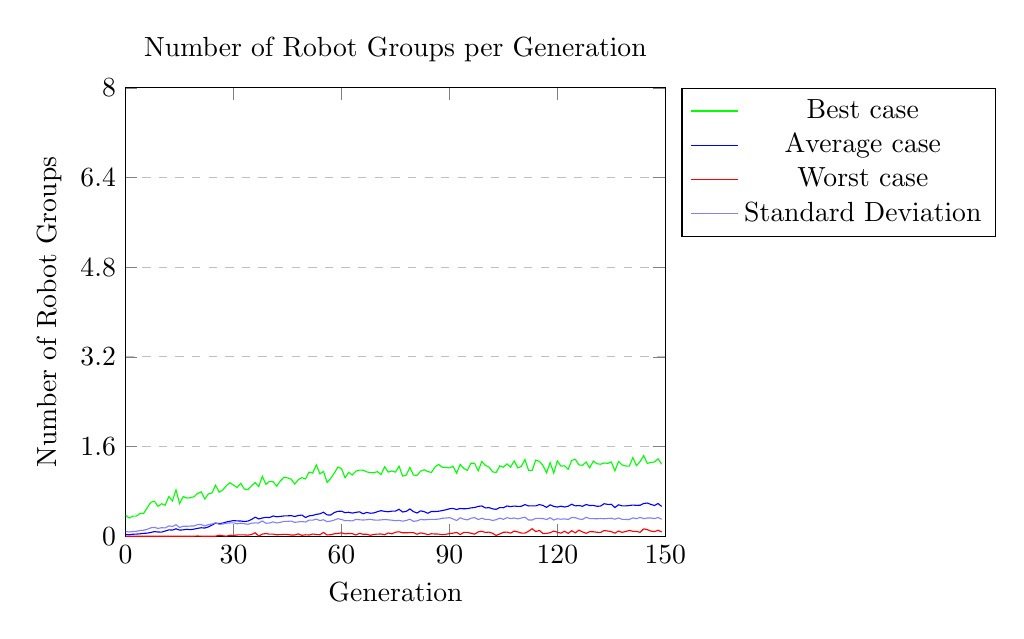
\begin{tikzpicture}
\begin{axis}[
	title={Number of Robot Groups per Generation},
	xlabel={Generation},
	ylabel={Number of Robot Groups},
	xmin=0, xmax=150,
	ymin=0, ymax=8,
	xtick={0.0,30.0,60.0,90.0,120.0,150.0},
	ytick={0.0,1.6,3.2,4.800000000000001,6.4,8.0},
	legend pos=outer north east,
	ymajorgrids=true,
	grid style=dashed,
]

\addplot[
	color=green,
	]
	coordinates {
	(0,0.375)(1,0.3241666666666666)(2,0.35875000000000007)(3,0.35875)(4,0.40525)(5,0.40583333333333327)(6,0.5060833333333332)(7,0.6054999999999998)(8,0.62325)(9,0.5330833333333332)(10,0.5793333333333333)(11,0.5531666666666666)(12,0.7072499999999998)(13,0.6299166666666666)(14,0.8267499999999999)(15,0.5819166666666665)(16,0.7083333333333331)(17,0.6804166666666664)(18,0.6868333333333334)(19,0.7039999999999998)(20,0.7630000000000001)(21,0.7915)(22,0.6628333333333335)(23,0.7529166666666666)(24,0.7726666666666666)(25,0.9098333333333334)(26,0.7850833333333334)(27,0.824)(28,0.9029999999999998)(29,0.9531666666666665)(30,0.9102500000000001)(31,0.86975)(32,0.9443333333333331)(33,0.8398333333333332)(34,0.8322499999999998)(35,0.9001666666666666)(36,0.9562499999999999)(37,0.8863333333333332)(38,1.0691666666666666)(39,0.9247499999999998)(40,0.9789999999999999)(41,0.9708333333333332)(42,0.8924166666666669)(43,0.9865833333333335)(44,1.0514166666666669)(45,1.0399166666666666)(46,1.0195833333333333)(47,0.93025)(48,1.0096666666666667)(49,1.0439999999999998)(50,1.0209166666666667)(51,1.1445833333333335)(52,1.1257500000000003)(53,1.2728333333333333)(54,1.1130833333333332)(55,1.1554999999999997)(56,0.9580833333333334)(57,1.0314166666666666)(58,1.1250833333333332)(59,1.2343333333333333)(60,1.2057499999999999)(61,1.0417500000000002)(62,1.1391666666666664)(63,1.0925)(64,1.1608333333333332)(65,1.1786666666666668)(66,1.1774166666666666)(67,1.1484999999999999)(68,1.1337499999999996)(69,1.1325833333333333)(70,1.1521666666666668)(71,1.10125)(72,1.237833333333333)(73,1.1429166666666668)(74,1.1653333333333336)(75,1.1438333333333333)(76,1.2491666666666668)(77,1.0725833333333334)(78,1.0910833333333332)(79,1.2281666666666669)(80,1.092)(81,1.0840833333333333)(82,1.1621666666666668)(83,1.1851666666666667)(84,1.1527500000000002)(85,1.1385833333333333)(86,1.2354166666666664)(87,1.28125)(88,1.2314166666666666)(89,1.2275833333333335)(90,1.218333333333333)(91,1.24875)(92,1.1230833333333334)(93,1.2809999999999997)(94,1.21)(95,1.1739166666666665)(96,1.303083333333333)(97,1.3001666666666667)(98,1.1651666666666667)(99,1.3323333333333331)(100,1.2624166666666667)(101,1.2346666666666666)(102,1.1486666666666663)(103,1.1369166666666666)(104,1.2554166666666662)(105,1.2311666666666665)(106,1.2890000000000006)(107,1.2331666666666665)(108,1.3441666666666665)(109,1.2186666666666663)(110,1.2461666666666669)(111,1.36925)(112,1.1736666666666669)(113,1.1748333333333332)(114,1.3591666666666669)(115,1.3355000000000004)(116,1.262333333333333)(117,1.1310833333333332)(118,1.31475)(119,1.1239166666666665)(120,1.34375)(121,1.2499999999999998)(122,1.2564999999999997)(123,1.1935)(124,1.3535833333333334)(125,1.372666666666667)(126,1.2715833333333333)(127,1.2659166666666666)(128,1.3231666666666668)(129,1.2197500000000001)(130,1.340583333333333)(131,1.2934166666666667)(132,1.2841666666666667)(133,1.3064166666666666)(134,1.2994166666666667)(135,1.3246666666666667)(136,1.1663333333333334)(137,1.33325)(138,1.2713333333333334)(139,1.25225)(140,1.2495833333333333)(141,1.4038333333333335)(142,1.259)(143,1.3324166666666666)(144,1.4386666666666665)(145,1.2990833333333338)(146,1.3167500000000003)(147,1.3242499999999997)(148,1.381166666666667)(149,1.285)
	};
	\addlegendentry{Best case}
\addplot[
	color=blue,
	]
	coordinates {
	(0,0.03088541666666666)(1,0.02609375)(2,0.03473611111111111)(3,0.037586805555555554)(4,0.04251736111111111)(5,0.05021527777777778)(6,0.05475347222222223)(7,0.06659375000000001)(8,0.08213541666666664)(9,0.07460763888888891)(10,0.07299652777777779)(11,0.09214583333333333)(12,0.11288194444444441)(13,0.10892708333333333)(14,0.13190625)(15,0.10883333333333335)(16,0.11338541666666666)(17,0.12359375000000002)(18,0.11641319444444444)(19,0.1260138888888889)(20,0.14006250000000003)(21,0.1506354166666667)(22,0.1452534722222222)(23,0.16597916666666662)(24,0.19839930555555557)(25,0.23294444444444445)(26,0.22588888888888892)(27,0.23382638888888885)(28,0.2537048611111111)(29,0.2667361111111111)(30,0.27820138888888885)(31,0.27260416666666665)(32,0.2712986111111112)(33,0.26249999999999996)(34,0.2699895833333333)(35,0.2986493055555556)(36,0.33863194444444444)(37,0.3081180555555555)(38,0.3250972222222223)(39,0.3365381944444444)(40,0.3326597222222222)(41,0.36065625)(42,0.3468055555555555)(43,0.35269097222222223)(44,0.3614027777777778)(45,0.36316666666666664)(46,0.366875)(47,0.3520381944444444)(48,0.36879166666666674)(49,0.3769201388888889)(50,0.33362152777777787)(51,0.36329513888888887)(52,0.3706041666666667)(53,0.3894444444444445)(54,0.3992916666666668)(55,0.4279374999999999)(56,0.3797152777777778)(57,0.3772638888888889)(58,0.4226354166666666)(59,0.44346875)(60,0.4466006944444445)(61,0.41924999999999996)(62,0.4273368055555556)(63,0.4118194444444445)(64,0.4252638888888889)(65,0.43505555555555553)(66,0.39984722222222213)(67,0.42368055555555556)(68,0.41002083333333333)(69,0.41530208333333335)(70,0.4376736111111111)(71,0.4558645833333334)(72,0.44282986111111106)(73,0.4359826388888889)(74,0.4466666666666667)(75,0.44826041666666666)(76,0.47943749999999996)(77,0.4313784722222222)(78,0.4436354166666667)(79,0.48618749999999994)(80,0.4385277777777779)(81,0.41406597222222213)(82,0.4524027777777778)(83,0.4380138888888888)(84,0.409)(85,0.44174652777777773)(86,0.4399895833333333)(87,0.44514930555555565)(88,0.4573645833333333)(89,0.4703541666666667)(90,0.48997222222222225)(91,0.49617708333333327)(92,0.47574652777777776)(93,0.4949236111111111)(94,0.4889756944444445)(95,0.49206597222222215)(96,0.5052743055555556)(97,0.511545138888889)(98,0.5314583333333334)(99,0.5401597222222222)(100,0.5040625)(101,0.5097395833333335)(102,0.4880555555555556)(103,0.4786805555555556)(104,0.5109618055555556)(105,0.5083055555555556)(106,0.5394131944444445)(107,0.5271874999999999)(108,0.5378298611111111)(109,0.5317534722222222)(110,0.533920138888889)(111,0.5643368055555557)(112,0.5398020833333333)(113,0.5398437500000001)(114,0.5401250000000001)(115,0.5641041666666666)(116,0.5489513888888888)(117,0.5143125000000001)(118,0.5594097222222223)(119,0.531892361111111)(120,0.5199756944444445)(121,0.5360763888888888)(122,0.5209930555555555)(123,0.5347638888888888)(124,0.5703819444444442)(125,0.5408923611111112)(126,0.5475034722222222)(127,0.5328159722222223)(128,0.5655347222222223)(129,0.547357638888889)(130,0.5492534722222221)(131,0.5340902777777778)(132,0.5363541666666667)(133,0.5794895833333334)(134,0.5680104166666666)(135,0.5692499999999999)(136,0.5107604166666667)(137,0.5607986111111111)(138,0.5402534722222223)(139,0.5406284722222222)(140,0.5476874999999999)(141,0.5555069444444445)(142,0.5508263888888889)(143,0.5520104166666666)(144,0.5829340277777778)(145,0.5920451388888889)(146,0.5668125)(147,0.5474826388888889)(148,0.5836319444444447)(149,0.5295034722222222)
	};
	\addlegendentry{Average case}
\addplot[
	color=red,
	]
	coordinates {
	(0,0.0)(1,0.0)(2,0.0)(3,0.0)(4,0.0)(5,0.0)(6,0.0)(7,0.0)(8,0.0)(9,0.0)(10,0.0)(11,0.0)(12,0.0)(13,0.0)(14,0.0)(15,0.0)(16,0.0)(17,0.0)(18,0.0)(19,0.0)(20,0.0035833333333333333)(21,0.0)(22,0.0)(23,0.0)(24,0.0)(25,0.0)(26,0.018833333333333334)(27,0.007666666666666667)(28,0.0003333333333333334)(29,0.0175)(30,0.014083333333333333)(31,0.022000000000000002)(32,0.024833333333333336)(33,0.02391666666666667)(34,0.01833333333333333)(35,0.03091666666666667)(36,0.06141666666666667)(37,0.0021666666666666666)(38,0.037)(39,0.04816666666666667)(40,0.035916666666666666)(41,0.03641666666666666)(42,0.024916666666666667)(43,0.028333333333333332)(44,0.0335)(45,0.03075)(46,0.020666666666666667)(47,0.021416666666666664)(48,0.04108333333333333)(49,0.015583333333333334)(50,0.025249999999999998)(51,0.021166666666666667)(52,0.03833333333333334)(53,0.031083333333333327)(54,0.025583333333333333)(55,0.06733333333333333)(56,0.021833333333333333)(57,0.02691666666666667)(58,0.04241666666666667)(59,0.049916666666666665)(60,0.05975)(61,0.040999999999999995)(62,0.04816666666666667)(63,0.045250000000000005)(64,0.02291666666666667)(65,0.050666666666666665)(66,0.0355)(67,0.034333333333333334)(68,0.016333333333333335)(69,0.030916666666666665)(70,0.03766666666666667)(71,0.03924999999999999)(72,0.026916666666666665)(73,0.05741666666666667)(74,0.04116666666666667)(75,0.07191666666666667)(76,0.07866666666666665)(77,0.060833333333333336)(78,0.06066666666666667)(79,0.06433333333333333)(80,0.06375000000000001)(81,0.03483333333333334)(82,0.05925)(83,0.047583333333333325)(84,0.028249999999999997)(85,0.04366666666666666)(86,0.03916666666666667)(87,0.038000000000000006)(88,0.027499999999999997)(89,0.034333333333333334)(90,0.0465)(91,0.05383333333333333)(92,0.06875)(93,0.029500000000000005)(94,0.06808333333333333)(95,0.0685)(96,0.052666666666666674)(97,0.036333333333333336)(98,0.07708333333333334)(99,0.08766666666666666)(100,0.06666666666666667)(101,0.07283333333333333)(102,0.050833333333333335)(103,0.013500000000000002)(104,0.04008333333333334)(105,0.06941666666666667)(106,0.07275)(107,0.05441666666666667)(108,0.09191666666666667)(109,0.07608333333333334)(110,0.05616666666666666)(111,0.05441666666666667)(112,0.08916666666666666)(113,0.13341666666666666)(114,0.08283333333333333)(115,0.10300000000000001)(116,0.04808333333333334)(117,0.049916666666666665)(118,0.062)(119,0.09125)(120,0.07016666666666667)(121,0.05425000000000001)(122,0.08775000000000001)(123,0.05116666666666667)(124,0.09725)(125,0.058916666666666666)(126,0.10816666666666666)(127,0.07516666666666667)(128,0.051666666666666666)(129,0.08083333333333334)(130,0.07941666666666666)(131,0.07041666666666667)(132,0.06666666666666667)(133,0.10108333333333333)(134,0.09258333333333334)(135,0.08166666666666668)(136,0.053916666666666675)(137,0.09233333333333334)(138,0.06841666666666665)(139,0.08308333333333333)(140,0.10241666666666664)(141,0.08725)(142,0.08524999999999999)(143,0.06891666666666668)(144,0.131)(145,0.11708333333333333)(146,0.09025000000000001)(147,0.08141666666666666)(148,0.10583333333333335)(149,0.07516666666666667)
	};
	\addlegendentry{Worst case}
\addplot[
	color=blue!50,
	]
	coordinates {
	(0,0.08624872357702378)(1,0.074887388019082)(2,0.08313141044355259)(3,0.0881437539943705)(4,0.10078105078703237)(5,0.10661422969848275)(6,0.12264228171764309)(7,0.14956352387065705)(8,0.15703374178878476)(9,0.1384343289102863)(10,0.15213016668563328)(11,0.14769818441031982)(12,0.18368916867897353)(13,0.17369846822315968)(14,0.2064640219879317)(15,0.15551395591455353)(16,0.17814514173500642)(17,0.17656877985499564)(18,0.18110456928919524)(19,0.1825113008153621)(20,0.2068309177876898)(21,0.20986159984656041)(22,0.18187615266398377)(23,0.2067022352148872)(24,0.21853639653683016)(25,0.24045420662522418)(26,0.2100462348704266)(27,0.21778765487413934)(28,0.23120654813895178)(29,0.2366285429021323)(30,0.23850901281251524)(31,0.22130717543638412)(32,0.23216147704177625)(33,0.2227407312907317)(34,0.21305352603493657)(35,0.23174237981749604)(36,0.23728550863600642)(37,0.23574574510156082)(38,0.27210922695782636)(39,0.23106812885772476)(40,0.23578716750355228)(41,0.2563010761144133)(42,0.23505498853364773)(43,0.2478952851133645)(44,0.26322810972016564)(45,0.2647251847339793)(46,0.2696911139758871)(47,0.24740062476736235)(48,0.2550171335269462)(49,0.26176179109819586)(50,0.25294734900060556)(51,0.2869163013741487)(52,0.28620487287600643)(53,0.30407200193662304)(54,0.27867450603852206)(55,0.2934470969542399)(56,0.2589682745564354)(57,0.26963338478989185)(58,0.2883355470881641)(59,0.31211500309898216)(60,0.29810992366259226)(61,0.2765109126754238)(62,0.27803804962148954)(63,0.27221760966016545)(64,0.3003796128903933)(65,0.29311034588336415)(66,0.28854693189632974)(67,0.2934019145359001)(68,0.3010885819912571)(69,0.2890741540247897)(70,0.28629012015671323)(71,0.29096317202908206)(72,0.2976966673928691)(73,0.2921085351439596)(74,0.2858172166288285)(75,0.27618912524151296)(76,0.2826182266367101)(77,0.26807419895932183)(78,0.2801451081370531)(79,0.30425349121332534)(80,0.2649865988807211)(81,0.2731850667826146)(82,0.29855952315895645)(83,0.29210020014176025)(84,0.2969833165401046)(85,0.30121101152503105)(86,0.3003080182003802)(87,0.3045773208252246)(88,0.319454210621114)(89,0.3234223967100451)(90,0.33203977139072316)(91,0.30806994635752155)(92,0.27976046363832074)(93,0.32850578701407995)(94,0.30390397319123397)(95,0.2913598119849496)(96,0.32077592525967014)(97,0.3325668331949649)(98,0.2978496787722862)(99,0.3206873505838111)(100,0.299821500953168)(101,0.30057255552523815)(102,0.27969913051446355)(103,0.29444380224789524)(104,0.32291203111119277)(105,0.30066696827287803)(106,0.3306602385120529)(107,0.31517776683917026)(108,0.3250340131802497)(109,0.30832562499501137)(110,0.3249875306189632)(111,0.3388492102490809)(112,0.28914429736895)(113,0.2879817607375189)(114,0.31910957211307844)(115,0.31787803816047744)(116,0.3150913213475822)(117,0.29610137005938575)(118,0.3300967942106481)(119,0.288493687903759)(120,0.3115981204518805)(121,0.30243505341153737)(122,0.3089956663349019)(123,0.29789467865195685)(124,0.3340913161016995)(125,0.3293683251667737)(126,0.3075669669326414)(127,0.2991071094508979)(128,0.33863270542512425)(129,0.31332285757973893)(130,0.3129824464662285)(131,0.3112193103372427)(132,0.3156146070404481)(133,0.3112847376855337)(134,0.3165029570828547)(135,0.32015214777847495)(136,0.3031568899126558)(137,0.32616205810836874)(138,0.3000230046760062)(139,0.29890308230581564)(140,0.2982761290848941)(141,0.3274410074861154)(142,0.31250742816934396)(143,0.3360850538933691)(144,0.3131439290183663)(145,0.3250501704851981)(146,0.3250043566203874)(147,0.3140447593931267)(148,0.3337075157572789)(149,0.3016294376462773)
	};
	\addlegendentry{Standard Deviation}
\end{axis}
\end{tikzpicture}
}
		\caption{Some sample caption}
	\end{subfigure}%
}
\\
\\
\\
\\
	\makebox[\linewidth][c]{%
	\begin{subfigure}[b]{0.7\textwidth}
		\centering
		\resizebox{0.9\linewidth}{!}{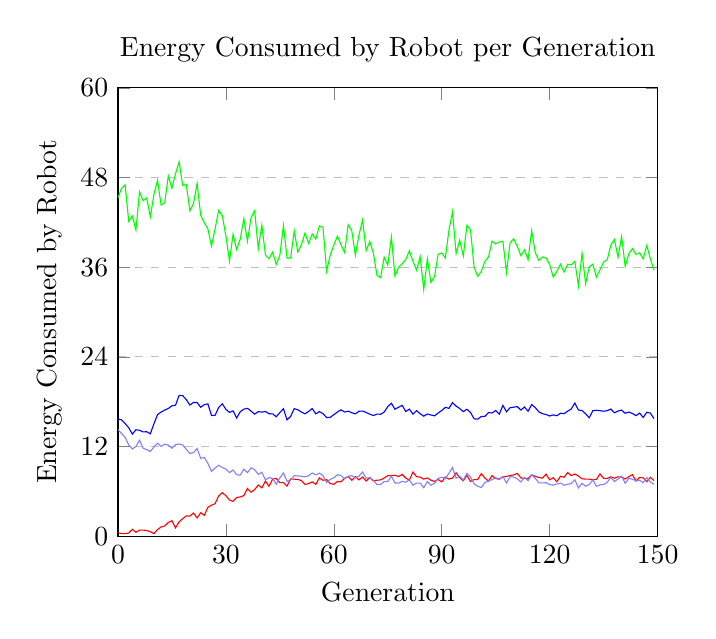
\begin{tikzpicture}
\begin{axis}[
	title={Energy Consumed by Robot per Generation},
	xlabel={Generation},
	ylabel={Energy Consumed by Robot},
	xmin=0, xmax=150,
	ymin=0, ymax=60,
	xtick={0.0,30.0,60.0,90.0,120.0,150.0},
	ytick={0.0,12.0,24.0,36.0,48.0,60.0},
	ymajorgrids=true,
	grid style=dashed,
]

\addplot[
	color=green,
	]
	coordinates {
	(0,45.26666666666666)(1,46.56666666666667)(2,47.016666666666666)(3,42.13333333333333)(4,42.85)(5,40.983333333333334)(6,46.10000000000001)(7,44.900000000000006)(8,45.26666666666667)(9,42.75)(10,45.733333333333334)(11,47.61666666666667)(12,44.31666666666666)(13,44.633333333333326)(14,48.21666666666667)(15,46.56666666666666)(16,48.483333333333334)(17,50.10000000000001)(18,46.96666666666667)(19,47.033333333333346)(20,43.55)(21,44.51666666666667)(22,47.21666666666667)(23,42.93333333333333)(24,41.96666666666666)(25,41.133333333333326)(26,38.833333333333336)(27,41.13333333333333)(28,43.60000000000001)(29,42.916666666666664)(30,40.19999999999999)(31,36.833333333333336)(32,40.41666666666667)(33,38.36666666666667)(34,39.76666666666666)(35,42.5)(36,39.48333333333333)(37,42.61666666666667)(38,43.56666666666666)(39,38.46666666666666)(40,41.633333333333326)(41,37.61666666666667)(42,37.13333333333333)(43,38.01666666666667)(44,36.36666666666667)(45,37.56666666666666)(46,41.56666666666668)(47,37.23333333333333)(48,37.233333333333334)(49,40.86666666666667)(50,38.03333333333333)(51,39.0)(52,40.56666666666666)(53,39.18333333333334)(54,40.45)(55,39.75)(56,41.53333333333333)(57,41.31666666666666)(58,35.5)(59,37.599999999999994)(60,38.949999999999996)(61,40.150000000000006)(62,39.016666666666666)(63,37.98333333333334)(64,41.68333333333333)(65,40.86666666666666)(66,37.6)(67,40.31666666666666)(68,42.33333333333334)(69,38.21666666666667)(70,39.45)(71,37.86666666666667)(72,34.916666666666664)(73,34.6)(74,37.33333333333334)(75,36.28333333333333)(76,40.033333333333324)(77,34.833333333333336)(78,35.983333333333334)(79,36.449999999999996)(80,37.016666666666666)(81,38.2)(82,36.8)(83,35.60000000000001)(84,37.416666666666664)(85,33.01666666666667)(86,37.11666666666667)(87,33.95)(88,34.71666666666667)(89,37.73333333333333)(90,37.9)(91,37.21666666666666)(92,40.95)(93,43.4)(94,37.81666666666666)(95,39.61666666666667)(96,37.51666666666667)(97,41.6)(98,41.0)(99,35.983333333333334)(100,34.766666666666666)(101,35.43333333333332)(102,36.78333333333333)(103,37.36666666666667)(104,39.483333333333334)(105,39.11666666666667)(106,39.36666666666666)(107,39.483333333333334)(108,35.31666666666666)(109,39.266666666666666)(110,39.800000000000004)(111,38.78333333333333)(112,37.55)(113,38.33333333333333)(114,37.0)(115,40.88333333333333)(116,37.96666666666666)(117,36.9)(118,37.36666666666667)(119,37.21666666666667)(120,36.35)(121,34.68333333333333)(122,35.43333333333333)(123,36.41666666666666)(124,35.35)(125,36.400000000000006)(126,36.300000000000004)(127,36.78333333333334)(128,33.48333333333334)(129,37.83333333333333)(130,33.83333333333333)(131,36.050000000000004)(132,36.416666666666664)(133,34.666666666666664)(134,35.65)(135,36.699999999999996)(136,36.99999999999999)(137,38.95)(138,39.71666666666666)(139,37.31666666666666)(140,40.1)(141,36.1)(142,37.76666666666666)(143,38.5)(144,37.71666666666666)(145,37.91666666666667)(146,37.11666666666667)(147,38.916666666666664)(148,37.099999999999994)(149,35.599999999999994)
	};
\addplot[
	color=blue,
	]
	coordinates {
	(0,15.677083333333337)(1,15.568749999999998)(2,15.077777777777778)(3,14.504166666666668)(4,13.6625)(5,14.241666666666665)(6,14.17152777777778)(7,13.954166666666666)(8,13.981944444444446)(9,13.696527777777778)(10,15.038194444444441)(11,16.26736111111111)(12,16.618055555555554)(13,16.875)(14,17.09513888888889)(15,17.45069444444444)(16,17.52708333333333)(17,18.844444444444445)(18,18.806944444444436)(19,18.28125)(20,17.55)(21,17.893055555555556)(22,17.89305555555556)(23,17.25625)(24,17.603472222222223)(25,17.707638888888887)(26,16.155555555555555)(27,16.179166666666664)(28,17.23611111111111)(29,17.722916666666666)(30,16.990972222222226)(31,16.569444444444443)(32,16.768055555555552)(33,15.824999999999998)(34,16.65555555555556)(35,17.006250000000005)(36,17.108333333333327)(37,16.73611111111111)(38,16.33194444444445)(39,16.664583333333336)(40,16.60625)(41,16.68888888888889)(42,16.38819444444444)(43,16.368055555555557)(44,15.984027777777778)(45,16.538888888888884)(46,17.060416666666665)(47,15.563194444444441)(48,16.03263888888889)(49,17.071527777777778)(50,16.92013888888889)(51,16.611111111111107)(52,16.381249999999998)(53,16.68680555555556)(54,17.081944444444446)(55,16.37013888888889)(56,16.680555555555554)(57,16.39375)(58,15.881250000000001)(59,15.906249999999998)(60,16.259722222222223)(61,16.613194444444446)(62,16.914583333333333)(63,16.6125)(64,16.72847222222222)(65,16.520833333333336)(66,16.374305555555555)(67,16.71944444444445)(68,16.74861111111111)(69,16.553472222222222)(70,16.32986111111111)(71,16.148611111111112)(72,16.344444444444445)(73,16.31736111111111)(74,16.615972222222222)(75,17.342361111111106)(76,17.787499999999998)(77,16.993055555555554)(78,17.256944444444446)(79,17.510416666666668)(80,16.68611111111111)(81,17.001388888888886)(82,16.334722222222222)(83,16.804166666666667)(84,16.387500000000003)(85,16.06111111111111)(86,16.346527777777776)(87,16.215277777777775)(88,16.10625)(89,16.48611111111111)(90,16.81041666666667)(91,17.24861111111111)(92,17.104166666666664)(93,17.875000000000004)(94,17.409027777777776)(95,17.077777777777776)(96,16.677083333333332)(97,16.990277777777777)(98,16.558333333333337)(99,15.701388888888886)(100,15.663888888888886)(101,16.018055555555552)(102,16.03472222222222)(103,16.540277777777774)(104,16.488194444444446)(105,16.825694444444444)(106,16.324305555555558)(107,17.507638888888888)(108,16.646527777777774)(109,17.19930555555555)(110,17.265972222222224)(111,17.346527777777776)(112,16.875)(113,17.28611111111111)(114,16.721527777777776)(115,17.625)(116,17.20347222222222)(117,16.635416666666668)(118,16.4)(119,16.281944444444445)(120,16.087500000000002)(121,16.2375)(122,16.117361111111112)(123,16.45416666666667)(124,16.38958333333333)(125,16.73125)(126,17.022222222222222)(127,17.815277777777776)(128,16.874305555555555)(129,16.82083333333333)(130,16.37777777777778)(131,15.850694444444445)(132,16.799999999999997)(133,16.852777777777778)(134,16.8)(135,16.720138888888886)(136,16.80625)(137,17.018055555555552)(138,16.51527777777778)(139,16.741666666666664)(140,16.880555555555556)(141,16.44027777777778)(142,16.620833333333334)(143,16.422916666666666)(144,16.13611111111111)(145,16.470833333333335)(146,15.8875)(147,16.588194444444444)(148,16.470833333333335)(149,15.741666666666662)
	};
\addplot[
	color=red,
	]
	coordinates {
	(0,0.44999999999999996)(1,0.35)(2,0.3333333333333333)(3,0.41666666666666663)(4,0.9166666666666671)(5,0.5166666666666666)(6,0.8166666666666669)(7,0.8166666666666669)(8,0.7500000000000002)(9,0.6166666666666667)(10,0.3333333333333333)(11,0.8833333333333333)(12,1.2333333333333334)(13,1.366666666666667)(14,1.8333333333333337)(15,2.0666666666666664)(16,1.1166666666666665)(17,1.9166666666666667)(18,2.349999999999999)(19,2.7166666666666663)(20,2.683333333333333)(21,3.0999999999999996)(22,2.4499999999999997)(23,3.1333333333333333)(24,2.7833333333333337)(25,3.8666666666666667)(26,4.15)(27,4.35)(28,5.383333333333334)(29,5.816666666666667)(30,5.433333333333332)(31,4.833333333333335)(32,4.666666666666666)(33,5.183333333333332)(34,5.25)(35,5.433333333333332)(36,6.383333333333333)(37,5.883333333333332)(38,6.233333333333332)(39,6.85)(40,6.466666666666666)(41,7.383333333333334)(42,6.666666666666667)(43,7.649999999999999)(44,7.733333333333333)(45,7.166666666666668)(46,7.166666666666667)(47,6.699999999999999)(48,7.65)(49,7.633333333333333)(50,7.583333333333332)(51,7.449999999999998)(52,6.916666666666666)(53,7.033333333333332)(54,7.2666666666666675)(55,6.933333333333334)(56,7.799999999999999)(57,7.483333333333333)(58,7.566666666666666)(59,7.049999999999998)(60,6.95)(61,7.300000000000001)(62,7.283333333333332)(63,7.750000000000001)(64,8.0)(65,7.483333333333334)(66,7.966666666666666)(67,7.533333333333332)(68,7.916666666666667)(69,7.383333333333333)(70,7.85)(71,7.3999999999999995)(72,7.483333333333334)(73,7.533333333333334)(74,7.783333333333332)(75,8.100000000000001)(76,8.1)(77,8.15)(78,8.0)(79,8.266666666666667)(80,7.783333333333333)(81,7.500000000000001)(82,8.583333333333334)(83,7.966666666666667)(84,7.899999999999999)(85,7.633333333333334)(86,7.800000000000001)(87,7.483333333333334)(88,7.333333333333334)(89,7.583333333333334)(90,7.266666666666667)(91,7.916666666666667)(92,7.633333333333334)(93,7.783333333333333)(94,8.466666666666665)(95,7.833333333333335)(96,7.416666666666669)(97,8.133333333333335)(98,7.3166666666666655)(99,7.566666666666666)(100,7.583333333333333)(101,8.366666666666667)(102,7.783333333333334)(103,7.366666666666667)(104,8.100000000000001)(105,7.716666666666666)(106,7.616666666666666)(107,7.933333333333332)(108,7.999999999999999)(109,8.116666666666669)(110,8.200000000000001)(111,8.399999999999999)(112,7.800000000000001)(113,7.733333333333332)(114,7.716666666666668)(115,8.216666666666669)(116,8.01666666666667)(117,7.8500000000000005)(118,7.766666666666667)(119,8.3)(120,7.55)(121,7.816666666666668)(122,7.283333333333334)(123,8.016666666666666)(124,7.883333333333334)(125,8.516666666666667)(126,8.116666666666665)(127,8.316666666666666)(128,8.05)(129,7.6833333333333345)(130,7.633333333333334)(131,7.633333333333335)(132,7.549999999999999)(133,7.600000000000001)(134,8.333333333333332)(135,7.733333333333333)(136,7.7333333333333325)(137,7.95)(138,7.749999999999999)(139,7.95)(140,7.916666666666669)(141,7.65)(142,7.966666666666666)(143,8.233333333333333)(144,7.383333333333333)(145,7.866666666666666)(146,7.816666666666666)(147,7.300000000000001)(148,7.866666666666665)(149,7.433333333333334)
	};
\addplot[
	color=blue!50,
	]
	coordinates {
	(0,14.280153822266879)(1,13.737996183551202)(2,13.231306390980691)(3,12.19778203796692)(4,11.674689715393813)(5,12.00728146954287)(6,12.838456273147793)(7,11.764501362355237)(8,11.584750566437005)(9,11.335487724267946)(10,11.931485898696163)(11,12.434112019371009)(12,12.030224588597003)(13,12.304351663468996)(14,12.184686816379807)(15,11.770172558134664)(16,12.240283134125841)(17,12.339379491751943)(18,12.20925711966199)(19,11.61120136335482)(20,11.078556951940604)(21,11.171922151851923)(22,11.752709350996827)(23,10.420322134414874)(24,10.535376535758335)(25,9.747443777617942)(26,8.667848426544825)(27,9.126212274287552)(28,9.488643408980636)(29,9.19476169738469)(30,8.9959890774235)(31,8.500750282900844)(32,8.864844622348313)(33,8.221378997692863)(34,8.173893678259061)(35,8.972378277025083)(36,8.499980903286795)(37,9.144092196042857)(38,8.900954509506207)(39,8.277542612989565)(40,8.550792749259704)(41,7.531690442441406)(42,7.855868352675383)(43,7.712193038429642)(44,6.944900958970443)(45,7.7876302359842615)(46,8.463621832342232)(47,7.3500830284798875)(48,7.5193637252012255)(49,8.106009555784706)(50,8.05629621726523)(51,8.024352121273473)(52,7.936180906802508)(53,8.092414874663472)(54,8.458063616809273)(55,8.212614643254248)(56,8.427727685698958)(57,8.101121436204668)(58,7.189444498369461)(59,7.597518310131954)(60,7.814410458285312)(61,8.22351587066587)(62,8.128333531833203)(63,7.656178701609447)(64,8.030250941129967)(65,8.100438629511473)(66,7.844333000696218)(67,8.042111980170352)(68,8.59268552838725)(69,7.766442672394701)(70,7.824825036997491)(71,7.5062288239330375)(72,6.88584050034114)(73,6.930904455577176)(74,7.310148184224493)(75,7.317841822906252)(76,8.046919525102986)(77,7.123933726162233)(78,7.098789107644505)(79,7.336950716443786)(80,7.223792876761637)(81,7.538631094276049)(82,6.824527283654105)(83,7.099961470457162)(84,7.109766896478448)(85,6.486845332355611)(86,7.315669892141451)(87,6.816591395202704)(88,7.088880676196245)(89,7.7340218068083235)(90,7.8826980922619505)(91,7.698057209077632)(92,8.407390106285291)(93,9.196164180149362)(94,7.7689007536619235)(95,8.001040988548862)(96,7.5225152311885655)(97,8.41583719226769)(98,7.92188807660878)(99,6.994491254367962)(100,6.675643645848624)(101,6.524157442715262)(102,7.171835540924859)(103,7.389413674105226)(104,7.56413785811107)(105,7.817006922765511)(106,7.6571405815118165)(107,8.000839058415915)(108,7.117391959656544)(109,7.976595356338731)(110,7.907535169658151)(111,7.680620320766394)(112,7.259393959940452)(113,7.864039027446746)(114,7.423073374412615)(115,8.222921450258402)(116,7.754244421011521)(117,7.131435874858751)(118,7.128500397445217)(119,7.153298629870321)(120,6.911105115647913)(121,6.8345688359265955)(122,6.981470417706145)(123,7.113760344629832)(124,6.815509411995631)(125,6.9614262452964715)(126,7.039322641615269)(127,7.5482976267391875)(128,6.4627190592426045)(129,7.072946527080282)(130,6.681878071604164)(131,6.920760551478433)(132,7.532217720956097)(133,6.664762392734871)(134,6.869821593469321)(135,6.916159094972801)(136,7.226629880223863)(137,7.850790841675324)(138,7.3199131706528116)(139,7.641254825303226)(140,8.015071506686894)(141,7.088871262160179)(142,7.728612367886719)(143,7.626685520819284)(144,7.4093598689017055)(145,7.489229310943266)(146,7.162497012536677)(147,7.831337816243148)(148,7.2684748891617375)(149,6.939704340184111)
	};
\end{axis}
\end{tikzpicture}
}
		\caption{Some sample caption}
	\end{subfigure}%
	\begin{subfigure}[b]{0.7\textwidth}
		\centering
		\resizebox{0.9\linewidth}{!}{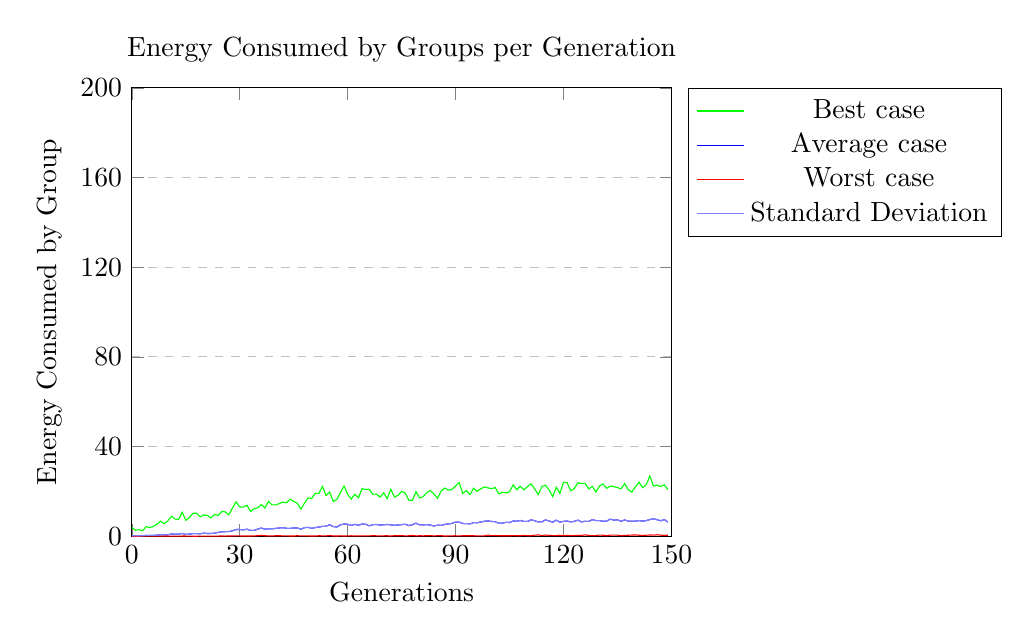
\begin{tikzpicture}
\begin{axis}[
	title={Energy Consumed by Groups per Generation},
	xlabel={Generations},
	ylabel={Energy Consumed by Group},
	xmin=0, xmax=150,
	ymin=0, ymax=200,
	xtick={0.0,30.0,60.0,90.0,120.0,150.0},
	ytick={0.0,40.0,80.0,120.0,160.0,200.0},
	legend pos=outer north east,
	ymajorgrids=true,
	grid style=dashed,
]

\addplot[
	color=green,
	]
	coordinates {
	(0,3.966666666666667)(1,2.666666666666667)(2,2.916666666666667)(3,2.433333333333333)(4,4.283333333333334)(5,3.833333333333333)(6,4.383333333333334)(7,5.383333333333334)(8,6.7)(9,5.549999999999999)(10,6.800000000000001)(11,8.883333333333335)(12,7.699999999999999)(13,7.433333333333334)(14,10.7)(15,7.083333333333332)(16,8.25)(17,10.233333333333334)(18,10.25)(19,8.683333333333334)(20,9.499999999999998)(21,9.266666666666667)(22,8.116666666666667)(23,9.766666666666666)(24,9.250000000000002)(25,11.016666666666667)(26,10.85)(27,9.516666666666667)(28,12.616666666666667)(29,15.316666666666668)(30,13.066666666666666)(31,12.95)(32,13.833333333333334)(33,11.033333333333335)(34,12.266666666666666)(35,12.666666666666666)(36,14.116666666666667)(37,12.566666666666663)(38,15.550000000000002)(39,13.950000000000001)(40,13.966666666666669)(41,14.533333333333333)(42,15.25)(43,14.9)(44,16.549999999999997)(45,15.533333333333333)(46,14.716666666666667)(47,12.066666666666666)(48,14.750000000000005)(49,17.066666666666666)(50,16.8)(51,19.15)(52,19.016666666666666)(53,22.199999999999996)(54,18.150000000000006)(55,19.683333333333337)(56,15.51666666666667)(57,16.416666666666668)(58,19.483333333333334)(59,22.366666666666664)(60,18.700000000000003)(61,16.583333333333332)(62,18.66666666666667)(63,17.15)(64,21.18333333333333)(65,20.916666666666668)(66,20.88333333333333)(67,18.733333333333334)(68,18.783333333333335)(69,17.433333333333334)(70,19.36666666666666)(71,16.75)(72,20.950000000000003)(73,17.500000000000004)(74,18.2)(75,19.950000000000003)(76,19.266666666666666)(77,16.06666666666667)(78,15.983333333333333)(79,19.8)(80,17.066666666666663)(81,17.599999999999998)(82,19.46666666666667)(83,20.350000000000005)(84,18.783333333333335)(85,16.883333333333333)(86,20.166666666666664)(87,21.48333333333333)(88,20.53333333333333)(89,20.849999999999998)(90,22.416666666666664)(91,23.9)(92,19.066666666666666)(93,20.35)(94,18.533333333333335)(95,21.383333333333336)(96,19.98333333333333)(97,21.150000000000002)(98,21.98333333333333)(99,21.55)(100,21.2)(101,21.716666666666672)(102,18.833333333333332)(103,19.6)(104,19.300000000000004)(105,19.8)(106,22.933333333333337)(107,20.700000000000006)(108,22.33333333333333)(109,20.65)(110,22.183333333333337)(111,23.366666666666667)(112,20.983333333333334)(113,18.616666666666667)(114,22.18333333333333)(115,22.733333333333334)(116,20.6)(117,17.633333333333333)(118,21.799999999999997)(119,19.13333333333333)(120,24.066666666666666)(121,23.900000000000006)(122,20.266666666666662)(123,21.249999999999996)(124,23.849999999999998)(125,23.483333333333334)(126,23.583333333333336)(127,21.1)(128,22.18333333333333)(129,19.68333333333334)(130,22.433333333333334)(131,23.283333333333335)(132,21.35)(133,22.400000000000002)(134,22.099999999999998)(135,21.683333333333337)(136,21.133333333333333)(137,23.483333333333334)(138,20.716666666666672)(139,19.700000000000006)(140,22.05)(141,24.050000000000004)(142,21.666666666666668)(143,22.983333333333338)(144,26.88333333333334)(145,22.383333333333336)(146,22.783333333333335)(147,22.13333333333333)(148,22.93333333333333)(149,20.816666666666674)
	};
	\addlegendentry{Best case}
\addplot[
	color=blue,
	]
	coordinates {
	(0,0.22291666666666662)(1,0.16805555555555554)(2,0.19652777777777777)(3,0.22291666666666662)(4,0.3291666666666666)(5,0.34930555555555554)(6,0.3659722222222222)(7,0.4576388888888888)(8,0.672222222222222)(9,0.6062499999999998)(10,0.5784722222222223)(11,0.9763888888888889)(12,0.9326388888888889)(13,0.8868055555555554)(14,1.2354166666666666)(15,0.7930555555555555)(16,0.9097222222222223)(17,1.1618055555555555)(18,1.15)(19,1.0583333333333333)(20,1.3479166666666669)(21,1.2118055555555556)(22,1.2125000000000001)(23,1.3416666666666668)(24,1.68125)(25,1.9770833333333333)(26,2.0131944444444447)(27,2.077083333333334)(28,2.394444444444444)(29,2.985416666666667)(30,2.9895833333333335)(31,2.793055555555556)(32,3.1444444444444444)(33,2.590277777777778)(34,2.6277777777777773)(35,3.153472222222223)(36,3.6486111111111117)(37,3.096527777777777)(38,3.3215277777777787)(39,3.3097222222222222)(40,3.4611111111111104)(41,3.6687500000000006)(42,3.7923611111111115)(43,3.5270833333333336)(44,3.470833333333333)(45,3.6868055555555554)(46,3.6562500000000004)(47,3.124305555555555)(48,3.80763888888889)(49,3.9618055555555567)(50,3.4875)(51,3.823611111111112)(52,4.097916666666667)(53,4.372222222222223)(54,4.426388888888888)(55,5.135416666666668)(56,4.290277777777778)(57,4.1201388888888895)(58,5.011805555555556)(59,5.450694444444444)(60,5.32638888888889)(61,4.809027777777779)(62,5.290972222222223)(63,4.878472222222223)(64,5.429166666666667)(65,5.322916666666666)(66,4.620833333333334)(67,5.151388888888889)(68,5.204861111111111)(69,4.992361111111111)(70,5.070833333333333)(71,5.243055555555557)(72,5.0625)(73,4.872916666666668)(74,5.013194444444443)(75,5.159722222222223)(76,5.315972222222223)(77,4.720833333333334)(78,5.11875)(79,5.82361111111111)(80,5.03263888888889)(81,5.022222222222222)(82,5.173611111111112)(83,4.9541666666666675)(84,4.56875)(85,4.902083333333334)(86,4.840972222222221)(87,5.247916666666669)(88,5.493055555555554)(89,5.6944444444444455)(90,6.309027777777777)(91,6.295833333333333)(92,5.6423611111111125)(93,5.634722222222221)(94,5.495833333333333)(95,6.0458333333333325)(96,6.009027777777777)(97,6.326388888888889)(98,6.659722222222223)(99,6.819444444444445)(100,6.5659722222222205)(101,6.459027777777777)(102,5.759027777777778)(103,5.812499999999999)(104,6.204166666666666)(105,6.1000000000000005)(106,6.786805555555555)(107,6.7145833333333345)(108,7.004166666666667)(109,6.588194444444445)(110,6.581944444444445)(111,7.308333333333333)(112,6.878472222222222)(113,6.3625)(114,6.4118055555555555)(115,7.247222222222222)(116,6.796527777777778)(117,6.230555555555554)(118,7.159027777777776)(119,6.275)(120,6.61875)(121,6.75902777777778)(122,6.371527777777778)(123,6.613194444444445)(124,7.162500000000001)(125,6.377083333333333)(126,6.654861111111112)(127,6.588888888888887)(128,7.391666666666666)(129,6.961111111111111)(130,6.950000000000001)(131,6.693055555555556)(132,6.723611111111111)(133,7.623611111111112)(134,7.152083333333332)(135,7.313194444444444)(136,6.606944444444446)(137,7.259027777777776)(138,6.7548611111111105)(139,6.678472222222221)(140,6.7138888888888895)(141,6.9527777777777775)(142,6.731250000000001)(143,6.954861111111112)(144,7.4319444444444445)(145,7.778472222222224)(146,7.363888888888889)(147,6.863888888888889)(148,7.436805555555557)(149,6.341666666666667)
	};
	\addlegendentry{Average case}
\addplot[
	color=red,
	]
	coordinates {
	(0,0.0)(1,0.0)(2,0.0)(3,0.03333333333333333)(4,0.03333333333333333)(5,0.03333333333333333)(6,0.03333333333333333)(7,0.03333333333333333)(8,0.0)(9,0.08333333333333333)(10,0.06666666666666667)(11,0.03333333333333333)(12,0.03333333333333333)(13,0.016666666666666666)(14,0.06666666666666667)(15,0.06666666666666667)(16,0.016666666666666666)(17,0.0)(18,0.0)(19,0.016666666666666666)(20,0.05)(21,0.03333333333333333)(22,0.016666666666666666)(23,0.05)(24,0.05)(25,0.09999999999999999)(26,0.05)(27,0.11666666666666667)(28,0.1)(29,0.16666666666666666)(30,0.11666666666666665)(31,0.08333333333333333)(32,0.11666666666666665)(33,0.06666666666666667)(34,0.13333333333333333)(35,0.21666666666666665)(36,0.36666666666666664)(37,0.18333333333333332)(38,0.16666666666666666)(39,0.08333333333333333)(40,0.19999999999999998)(41,0.18333333333333335)(42,0.16666666666666666)(43,0.16666666666666666)(44,0.08333333333333333)(45,0.08333333333333333)(46,0.21666666666666665)(47,0.11666666666666667)(48,0.11666666666666667)(49,0.15)(50,0.06666666666666667)(51,0.06666666666666667)(52,0.2)(53,0.15000000000000002)(54,0.13333333333333333)(55,0.3)(56,0.11666666666666667)(57,0.06666666666666667)(58,0.18333333333333332)(59,0.08333333333333334)(60,0.13333333333333333)(61,0.18333333333333332)(62,0.09999999999999999)(63,0.15)(64,0.16666666666666669)(65,0.11666666666666667)(66,0.11666666666666665)(67,0.26666666666666666)(68,0.16666666666666666)(69,0.16666666666666666)(70,0.16666666666666666)(71,0.19999999999999998)(72,0.08333333333333333)(73,0.2333333333333333)(74,0.18333333333333335)(75,0.24999999999999997)(76,0.13333333333333333)(77,0.18333333333333332)(78,0.35)(79,0.13333333333333333)(80,0.19999999999999998)(81,0.16666666666666666)(82,0.19999999999999998)(83,0.26666666666666666)(84,0.11666666666666667)(85,0.2333333333333333)(86,0.2833333333333333)(87,0.05)(88,0.13333333333333333)(89,0.16666666666666666)(90,0.18333333333333332)(91,0.11666666666666665)(92,0.19999999999999998)(93,0.2)(94,0.18333333333333332)(95,0.2)(96,0.13333333333333333)(97,0.11666666666666667)(98,0.13333333333333333)(99,0.5)(100,0.21666666666666667)(101,0.3)(102,0.19999999999999998)(103,0.2)(104,0.2)(105,0.18333333333333332)(106,0.25)(107,0.21666666666666665)(108,0.2)(109,0.3833333333333333)(110,0.2333333333333333)(111,0.2)(112,0.45)(113,0.5833333333333334)(114,0.26666666666666666)(115,0.5333333333333333)(116,0.3)(117,0.2833333333333333)(118,0.25000000000000006)(119,0.43333333333333335)(120,0.18333333333333335)(121,0.4)(122,0.24999999999999997)(123,0.26666666666666666)(124,0.36666666666666664)(125,0.31666666666666665)(126,0.6)(127,0.35)(128,0.26666666666666666)(129,0.26666666666666666)(130,0.49999999999999994)(131,0.4333333333333333)(132,0.21666666666666665)(133,0.44999999999999996)(134,0.4666666666666666)(135,0.4666666666666666)(136,0.2)(137,0.3333333333333333)(138,0.41666666666666663)(139,0.5166666666666667)(140,0.5666666666666667)(141,0.43333333333333335)(142,0.3333333333333333)(143,0.43333333333333335)(144,0.55)(145,0.4666666666666667)(146,0.6500000000000001)(147,0.45)(148,0.3833333333333333)(149,0.4166666666666667)
	};
	\addlegendentry{Worst case}
\addplot[
	color=blue!50,
	]
	coordinates {
	(0,0.22291666666666662)(1,0.16805555555555554)(2,0.19652777777777777)(3,0.22291666666666662)(4,0.3291666666666666)(5,0.34930555555555554)(6,0.3659722222222222)(7,0.4576388888888888)(8,0.672222222222222)(9,0.6062499999999998)(10,0.5784722222222223)(11,0.9763888888888889)(12,0.9326388888888889)(13,0.8868055555555554)(14,1.2354166666666666)(15,0.7930555555555555)(16,0.9097222222222223)(17,1.1618055555555555)(18,1.15)(19,1.0583333333333333)(20,1.3479166666666669)(21,1.2118055555555556)(22,1.2125000000000001)(23,1.3416666666666668)(24,1.68125)(25,1.9770833333333333)(26,2.0131944444444447)(27,2.077083333333334)(28,2.394444444444444)(29,2.985416666666667)(30,2.9895833333333335)(31,2.793055555555556)(32,3.1444444444444444)(33,2.590277777777778)(34,2.6277777777777773)(35,3.153472222222223)(36,3.6486111111111117)(37,3.096527777777777)(38,3.3215277777777787)(39,3.3097222222222222)(40,3.4611111111111104)(41,3.6687500000000006)(42,3.7923611111111115)(43,3.5270833333333336)(44,3.470833333333333)(45,3.6868055555555554)(46,3.6562500000000004)(47,3.124305555555555)(48,3.80763888888889)(49,3.9618055555555567)(50,3.4875)(51,3.823611111111112)(52,4.097916666666667)(53,4.372222222222223)(54,4.426388888888888)(55,5.135416666666668)(56,4.290277777777778)(57,4.1201388888888895)(58,5.011805555555556)(59,5.450694444444444)(60,5.32638888888889)(61,4.809027777777779)(62,5.290972222222223)(63,4.878472222222223)(64,5.429166666666667)(65,5.322916666666666)(66,4.620833333333334)(67,5.151388888888889)(68,5.204861111111111)(69,4.992361111111111)(70,5.070833333333333)(71,5.243055555555557)(72,5.0625)(73,4.872916666666668)(74,5.013194444444443)(75,5.159722222222223)(76,5.315972222222223)(77,4.720833333333334)(78,5.11875)(79,5.82361111111111)(80,5.03263888888889)(81,5.022222222222222)(82,5.173611111111112)(83,4.9541666666666675)(84,4.56875)(85,4.902083333333334)(86,4.840972222222221)(87,5.247916666666669)(88,5.493055555555554)(89,5.6944444444444455)(90,6.309027777777777)(91,6.295833333333333)(92,5.6423611111111125)(93,5.634722222222221)(94,5.495833333333333)(95,6.0458333333333325)(96,6.009027777777777)(97,6.326388888888889)(98,6.659722222222223)(99,6.819444444444445)(100,6.5659722222222205)(101,6.459027777777777)(102,5.759027777777778)(103,5.812499999999999)(104,6.204166666666666)(105,6.1000000000000005)(106,6.786805555555555)(107,6.7145833333333345)(108,7.004166666666667)(109,6.588194444444445)(110,6.581944444444445)(111,7.308333333333333)(112,6.878472222222222)(113,6.3625)(114,6.4118055555555555)(115,7.247222222222222)(116,6.796527777777778)(117,6.230555555555554)(118,7.159027777777776)(119,6.275)(120,6.61875)(121,6.75902777777778)(122,6.371527777777778)(123,6.613194444444445)(124,7.162500000000001)(125,6.377083333333333)(126,6.654861111111112)(127,6.588888888888887)(128,7.391666666666666)(129,6.961111111111111)(130,6.950000000000001)(131,6.693055555555556)(132,6.723611111111111)(133,7.623611111111112)(134,7.152083333333332)(135,7.313194444444444)(136,6.606944444444446)(137,7.259027777777776)(138,6.7548611111111105)(139,6.678472222222221)(140,6.7138888888888895)(141,6.9527777777777775)(142,6.731250000000001)(143,6.954861111111112)(144,7.4319444444444445)(145,7.778472222222224)(146,7.363888888888889)(147,6.863888888888889)(148,7.436805555555557)(149,6.341666666666667)
	};
	\addlegendentry{Standard Deviation}
\end{axis}
\end{tikzpicture}
}
		\caption{Some sample caption}
	\end{subfigure}%
}
\caption{Figure shows results from a 3 connection port simulation (p.2)}
\end{figure}


\newpage

\vspace*{-2.0cm}
\textbf{\Huge LARGE SAMPLE HEADER}
\vspace{1.5cm}
\begin{tikzpicture}[remember picture,overlay]
   \node[anchor=south east,inner sep=20pt] at (current page.south east)
              {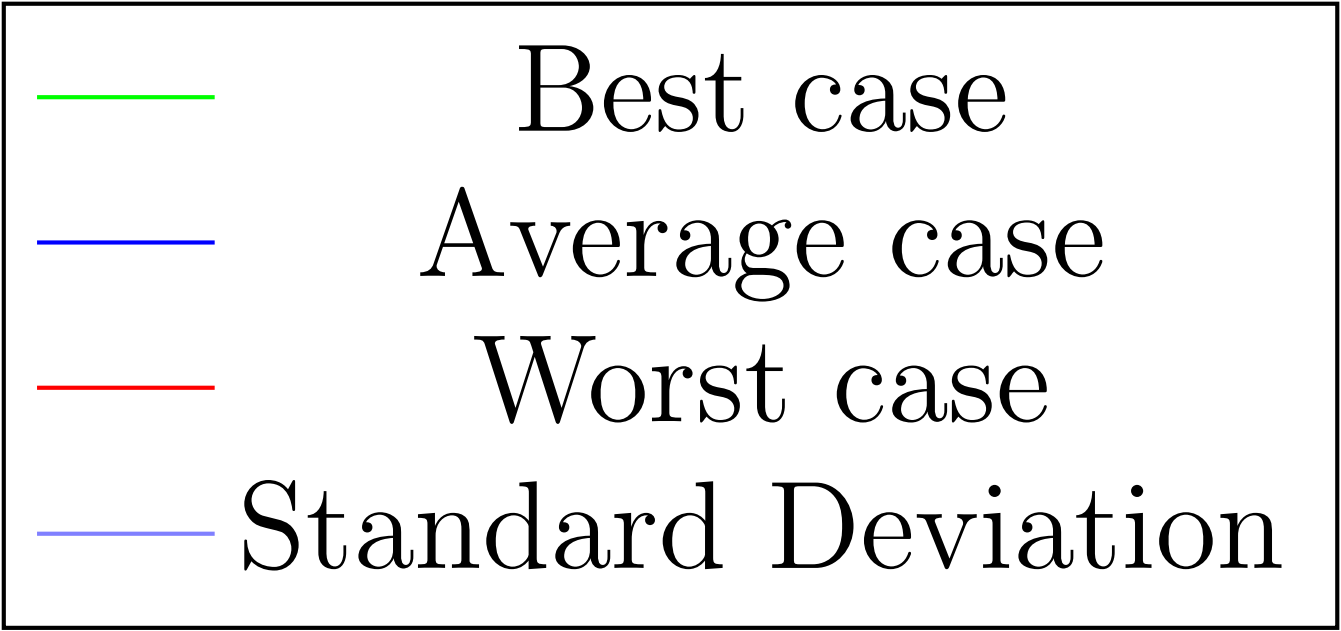
\includegraphics[scale=0.1]{chapters/res/generated_graph_legend.png}};
\end{tikzpicture}

\begin{figure}[H]
\vspace*{-1cm}
	\makebox[\linewidth][c]{%
	\begin{subfigure}[b]{0.7\textwidth}
		\label{test1}
		\centering
		\resizebox{0.9\linewidth}{!}{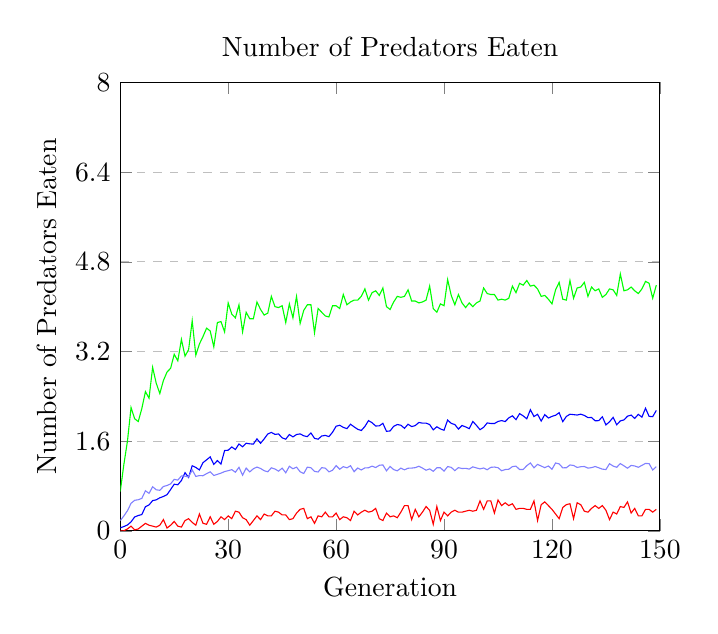
\begin{tikzpicture}
\begin{axis}[
	title={Number of Predators Eaten},
	xlabel={Generation},
	ylabel={Number of Predators Eaten},
	xmin=0, xmax=150,
	ymin=0, ymax=8,
	xtick={0.0,30.0,60.0,90.0,120.0,150.0},
	ytick={0.0,1.6,3.2,4.800000000000001,6.4,8.0},
	ymajorgrids=true,
	grid style=dashed,
]

\addplot[
	color=green,
	]
	coordinates {
	(0,0.7000000000000001)(1,1.1833333333333333)(2,1.6)(3,2.1999999999999997)(4,2.0)(5,1.95)(6,2.183333333333333)(7,2.483333333333334)(8,2.3666666666666663)(9,2.9166666666666665)(10,2.6333333333333333)(11,2.45)(12,2.683333333333334)(13,2.833333333333333)(14,2.9)(15,3.1499999999999995)(16,3.033333333333333)(17,3.4166666666666665)(18,3.1166666666666667)(19,3.233333333333333)(20,3.7499999999999996)(21,3.1333333333333337)(22,3.333333333333333)(23,3.4666666666666663)(24,3.616666666666667)(25,3.5666666666666664)(26,3.2833333333333328)(27,3.7166666666666672)(28,3.733333333333334)(29,3.55)(30,4.066666666666667)(31,3.866666666666667)(32,3.8)(33,4.033333333333333)(34,3.55)(35,3.9)(36,3.7833333333333337)(37,3.7833333333333328)(38,4.083333333333333)(39,3.95)(40,3.8499999999999996)(41,3.883333333333333)(42,4.183333333333333)(43,4.0)(44,3.983333333333333)(45,4.016666666666666)(46,3.7166666666666663)(47,4.05)(48,3.8)(49,4.183333333333333)(50,3.7)(51,3.9333333333333327)(52,4.033333333333333)(53,4.033333333333333)(54,3.533333333333333)(55,3.9666666666666663)(56,3.9)(57,3.8333333333333335)(58,3.816666666666667)(59,4.016666666666667)(60,4.016666666666667)(61,3.966666666666667)(62,4.216666666666666)(63,4.033333333333333)(64,4.083333333333333)(65,4.116666666666666)(66,4.116666666666666)(67,4.183333333333333)(68,4.316666666666666)(69,4.116666666666667)(70,4.25)(71,4.283333333333333)(72,4.2)(73,4.333333333333333)(74,3.9999999999999996)(75,3.95)(76,4.083333333333334)(77,4.183333333333333)(78,4.166666666666666)(79,4.183333333333334)(80,4.300000000000001)(81,4.1)(82,4.1)(83,4.066666666666667)(84,4.083333333333333)(85,4.116666666666666)(86,4.366666666666666)(87,3.9666666666666672)(88,3.8999999999999995)(89,4.050000000000001)(90,4.016666666666667)(91,4.483333333333333)(92,4.2)(93,4.033333333333333)(94,4.216666666666667)(95,4.066666666666666)(96,3.983333333333334)(97,4.066666666666666)(98,3.999999999999999)(99,4.066666666666666)(100,4.1)(101,4.333333333333333)(102,4.233333333333333)(103,4.216666666666667)(104,4.216666666666667)(105,4.116666666666666)(106,4.133333333333334)(107,4.116666666666666)(108,4.1499999999999995)(109,4.366666666666666)(110,4.25)(111,4.416666666666667)(112,4.383333333333333)(113,4.466666666666667)(114,4.366666666666667)(115,4.383333333333334)(116,4.316666666666667)(117,4.183333333333333)(118,4.2)(119,4.133333333333333)(120,4.05)(121,4.3)(122,4.433333333333333)(123,4.133333333333334)(124,4.116666666666667)(125,4.466666666666667)(126,4.15)(127,4.333333333333333)(128,4.35)(129,4.433333333333334)(130,4.183333333333334)(131,4.35)(132,4.283333333333333)(133,4.316666666666666)(134,4.166666666666666)(135,4.216666666666667)(136,4.316666666666666)(137,4.3)(138,4.2)(139,4.583333333333333)(140,4.283333333333334)(141,4.3)(142,4.35)(143,4.283333333333333)(144,4.233333333333333)(145,4.316666666666666)(146,4.45)(147,4.416666666666666)(148,4.1499999999999995)(149,4.383333333333333)
	};
\addplot[
	color=blue,
	]
	coordinates {
	(0,0.05208333333333333)(1,0.07638888888888888)(2,0.10416666666666667)(3,0.15972222222222218)(4,0.2472222222222222)(5,0.2729166666666667)(6,0.29027777777777775)(7,0.4305555555555556)(8,0.4618055555555555)(9,0.5395833333333333)(10,0.5527777777777777)(11,0.5895833333333331)(12,0.6125)(13,0.6451388888888889)(14,0.7368055555555553)(15,0.8319444444444444)(16,0.8222222222222223)(17,0.8979166666666666)(18,1.0374999999999999)(19,0.9527777777777778)(20,1.1611111111111112)(21,1.13125)(22,1.086111111111111)(23,1.215972222222222)(24,1.2666666666666666)(25,1.3194444444444442)(26,1.1854166666666666)(27,1.2534722222222225)(28,1.192361111111111)(29,1.4326388888888892)(30,1.4381944444444443)(31,1.4958333333333333)(32,1.4513888888888888)(33,1.5493055555555553)(34,1.4993055555555557)(35,1.5625)(36,1.5520833333333333)(37,1.5472222222222225)(38,1.6409722222222223)(39,1.5618055555555557)(40,1.6402777777777782)(41,1.7277777777777776)(42,1.75625)(43,1.7208333333333334)(44,1.728472222222222)(45,1.6590277777777778)(46,1.6347222222222222)(47,1.71875)(48,1.676388888888889)(49,1.7187500000000004)(50,1.729861111111111)(51,1.6958333333333335)(52,1.6805555555555558)(53,1.745138888888889)(54,1.65)(55,1.6354166666666667)(56,1.691666666666667)(57,1.703472222222222)(58,1.6812500000000001)(59,1.758333333333333)(60,1.8659722222222224)(61,1.8840277777777779)(62,1.8458333333333334)(63,1.823611111111111)(64,1.902083333333333)(65,1.8548611111111115)(66,1.8125)(67,1.7895833333333335)(68,1.8618055555555557)(69,1.9666666666666663)(70,1.9284722222222221)(71,1.8701388888888888)(72,1.8729166666666668)(73,1.918055555555556)(74,1.7756944444444445)(75,1.7819444444444443)(76,1.8652777777777774)(77,1.896527777777778)(78,1.8847222222222226)(79,1.829166666666667)(80,1.9020833333333331)(81,1.8597222222222225)(82,1.877777777777778)(83,1.9333333333333331)(84,1.9215277777777777)(85,1.9215277777777775)(86,1.8965277777777774)(87,1.8013888888888887)(88,1.8569444444444443)(89,1.8173611111111108)(90,1.7951388888888888)(91,1.9770833333333329)(92,1.9166666666666667)(93,1.8965277777777776)(94,1.815277777777778)(95,1.8798611111111112)(96,1.8541666666666665)(97,1.823611111111111)(98,1.9513888888888886)(99,1.882638888888889)(100,1.8041666666666667)(101,1.8472222222222223)(102,1.9256944444444442)(103,1.915277777777778)(104,1.9138888888888888)(105,1.9513888888888886)(106,1.967361111111111)(107,1.9493055555555556)(108,2.015277777777778)(109,2.051388888888889)(110,1.9840277777777775)(111,2.0909722222222222)(112,2.0506944444444444)(113,1.9986111111111113)(114,2.161111111111111)(115,2.0395833333333333)(116,2.079861111111111)(117,1.9590277777777776)(118,2.073611111111111)(119,2.0125)(120,2.0416666666666665)(121,2.0625)(122,2.107638888888889)(123,1.9479166666666667)(124,2.0409722222222224)(125,2.079861111111111)(126,2.0736111111111115)(127,2.0659722222222223)(128,2.08125)(129,2.0590277777777777)(130,2.020138888888889)(131,2.0222222222222226)(132,1.9631944444444445)(133,1.965972222222222)(134,2.0354166666666664)(135,1.8902777777777777)(136,1.945833333333333)(137,2.024305555555555)(138,1.8923611111111112)(139,1.9618055555555558)(140,1.978472222222222)(141,2.045138888888889)(142,2.0652777777777778)(143,2.0055555555555555)(144,2.0784722222222225)(145,2.0284722222222227)(146,2.1875000000000004)(147,2.042361111111111)(148,2.0368055555555555)(149,2.1479166666666667)
	};
\addplot[
	color=red,
	]
	coordinates {
	(0,0.0)(1,0.0)(2,0.03333333333333333)(3,0.08333333333333333)(4,0.016666666666666666)(5,0.03333333333333333)(6,0.08333333333333333)(7,0.13333333333333333)(8,0.1)(9,0.08333333333333333)(10,0.06666666666666667)(11,0.1)(12,0.19999999999999998)(13,0.05)(14,0.1)(15,0.16666666666666666)(16,0.08333333333333333)(17,0.06666666666666667)(18,0.18333333333333332)(19,0.21666666666666665)(20,0.15)(21,0.1)(22,0.3)(23,0.13333333333333333)(24,0.11666666666666667)(25,0.24999999999999997)(26,0.11666666666666667)(27,0.16666666666666666)(28,0.24999999999999997)(29,0.19999999999999998)(30,0.26666666666666666)(31,0.21666666666666665)(32,0.35)(33,0.3333333333333333)(34,0.23333333333333334)(35,0.19999999999999998)(36,0.09999999999999999)(37,0.18333333333333332)(38,0.26666666666666666)(39,0.2)(40,0.3)(41,0.26666666666666666)(42,0.26666666666666666)(43,0.35)(44,0.33333333333333337)(45,0.2833333333333333)(46,0.2833333333333333)(47,0.19999999999999998)(48,0.21666666666666665)(49,0.31666666666666665)(50,0.3833333333333333)(51,0.39999999999999997)(52,0.21666666666666665)(53,0.25)(54,0.13333333333333333)(55,0.26666666666666666)(56,0.25)(57,0.3333333333333333)(58,0.25)(59,0.25)(60,0.31666666666666665)(61,0.19999999999999998)(62,0.24999999999999997)(63,0.2333333333333333)(64,0.18333333333333332)(65,0.35)(66,0.2833333333333333)(67,0.3333333333333333)(68,0.36666666666666664)(69,0.3333333333333333)(70,0.35)(71,0.39999999999999997)(72,0.21666666666666665)(73,0.18333333333333335)(74,0.31666666666666665)(75,0.25)(76,0.26666666666666666)(77,0.2333333333333333)(78,0.3333333333333333)(79,0.44999999999999996)(80,0.44999999999999996)(81,0.19999999999999998)(82,0.3833333333333333)(83,0.25)(84,0.3333333333333333)(85,0.4333333333333333)(86,0.36666666666666664)(87,0.11666666666666667)(88,0.43333333333333335)(89,0.18333333333333332)(90,0.3333333333333333)(91,0.26666666666666666)(92,0.33333333333333337)(93,0.36666666666666664)(94,0.3333333333333333)(95,0.33333333333333337)(96,0.35)(97,0.36666666666666664)(98,0.35)(99,0.36666666666666664)(100,0.5333333333333333)(101,0.3833333333333333)(102,0.5333333333333334)(103,0.5333333333333334)(104,0.31666666666666665)(105,0.55)(106,0.44999999999999996)(107,0.49999999999999994)(108,0.45)(109,0.4833333333333333)(110,0.3833333333333333)(111,0.39999999999999997)(112,0.39999999999999997)(113,0.3833333333333333)(114,0.3833333333333333)(115,0.5333333333333333)(116,0.18333333333333335)(117,0.4666666666666667)(118,0.5166666666666667)(119,0.44999999999999996)(120,0.3833333333333333)(121,0.3)(122,0.21666666666666665)(123,0.41666666666666663)(124,0.4666666666666666)(125,0.4833333333333333)(126,0.21666666666666667)(127,0.5)(128,0.4666666666666666)(129,0.35)(130,0.3333333333333333)(131,0.39999999999999997)(132,0.44999999999999996)(133,0.39999999999999997)(134,0.44999999999999996)(135,0.36666666666666664)(136,0.19999999999999998)(137,0.3333333333333333)(138,0.3)(139,0.4333333333333333)(140,0.41666666666666663)(141,0.5166666666666667)(142,0.31666666666666665)(143,0.39999999999999997)(144,0.26666666666666666)(145,0.26666666666666666)(146,0.3833333333333333)(147,0.3833333333333333)(148,0.33333333333333337)(149,0.3833333333333333)
	};
\addplot[
	color=blue!50,
	]
	coordinates {
	(0,0.18278838774740638)(1,0.2650161413739076)(2,0.3587928839925453)(3,0.4900821703296627)(4,0.54459727410782)(5,0.5545685968017638)(6,0.5792593398430832)(7,0.71388775401913)(8,0.6680153745954598)(9,0.7862661663021089)(10,0.7323322711294675)(11,0.7232798741035663)(12,0.7907678001210371)(13,0.8090166745285634)(14,0.8371326083319258)(15,0.9190028980484045)(16,0.9044356882461582)(17,0.9804491056396011)(18,0.9748014461995888)(19,0.9610174284836147)(20,1.0867987791328535)(21,0.9709079492692209)(22,0.9853234267997043)(23,0.9831259835154913)(24,1.0206058573371166)(25,1.0515330141539319)(26,0.9875336274994478)(27,1.0076874183058235)(28,1.029444268654703)(29,1.056869419165187)(30,1.0732837792813779)(31,1.0914060339663927)(32,1.0460620176961581)(33,1.1333405871601774)(34,0.9931882172242027)(35,1.1184970709493312)(36,1.0516856277089284)(37,1.1077719175062815)(38,1.1374374880648153)(39,1.1125837293032494)(40,1.0728987427941858)(41,1.0530961657713889)(42,1.1245529229783857)(43,1.1030027652445755)(44,1.0648559776125044)(45,1.1180841294734576)(46,1.0353279113840619)(47,1.1515583374825373)(48,1.1075866277392334)(49,1.1361137220811768)(50,1.054104441051161)(51,1.0228183219636515)(52,1.1361450521563616)(53,1.1257190225108844)(54,1.0603107201058808)(55,1.0498866928433734)(56,1.127289231045117)(57,1.1177886672994757)(58,1.052114515037439)(59,1.079956706069617)(60,1.1632661161087476)(61,1.0986896191818356)(62,1.1450962357872447)(63,1.1232396296585718)(64,1.1616122167882375)(65,1.0561475426094742)(66,1.1200179168008249)(67,1.0860115843462976)(68,1.122787741984332)(69,1.1249209692378408)(70,1.1542918467618977)(71,1.1287147745741566)(72,1.1692597303488006)(73,1.1760774554025517)(74,1.0696991357625123)(75,1.1483880114005034)(76,1.0925941502896968)(77,1.0713631335862495)(78,1.1185068077632454)(79,1.0881694770785282)(80,1.1168308152866193)(81,1.1196551698862574)(82,1.1270831702413753)(83,1.151688211543874)(84,1.1195240865495644)(85,1.0813205754720165)(86,1.1048076862707619)(87,1.0620584575315666)(88,1.125721178992391)(89,1.1245575351746147)(90,1.064596008946544)(91,1.146214885443953)(92,1.1328206765386273)(93,1.074384762450931)(94,1.127386686000854)(95,1.1112309381885566)(96,1.1152974307809338)(97,1.1008980726718103)(98,1.1419659935051305)(99,1.1223782301709626)(100,1.1046337544955327)(101,1.1206544644575285)(102,1.0895299397388558)(103,1.1327690859811637)(104,1.1380969850220921)(105,1.1258992517956732)(106,1.0724549783471382)(107,1.0935454059375591)(108,1.0986094147506422)(109,1.145515983286847)(110,1.1549187331411999)(111,1.0936318642892884)(112,1.0951159004133653)(113,1.162060252298575)(114,1.2101478535313062)(115,1.1253816911236827)(116,1.1851473363614888)(117,1.156483377235358)(118,1.1260092016519)(119,1.1574926718533987)(120,1.0985324322116712)(121,1.2103425107205892)(122,1.1940351269614047)(123,1.1236776877151105)(124,1.126008365632153)(125,1.1748218396980867)(126,1.1663666524162417)(127,1.1310319324020974)(128,1.1436976992417742)(129,1.1478742000997693)(130,1.1187309326503099)(131,1.127299822382476)(132,1.147719571045176)(133,1.124638308031614)(134,1.1006821903279815)(135,1.092966772107917)(136,1.1976236991713707)(137,1.1552425908971318)(138,1.1341063615860247)(139,1.1994478517733465)(140,1.1600982940858218)(141,1.1169661760816088)(142,1.1668815443285074)(143,1.1571308890999008)(144,1.1336891403934988)(145,1.1678650459191762)(146,1.2029839675213825)(147,1.1983992780231874)(148,1.0853026692707464)(149,1.1447271801086958)
	};
\end{axis}
\end{tikzpicture}
}
		\caption{Some sample caption}
	\end{subfigure}%
	\begin{subfigure}[b]{0.7\textwidth}
		\label{test2}		
		\centering
		\resizebox{0.9\linewidth}{!}{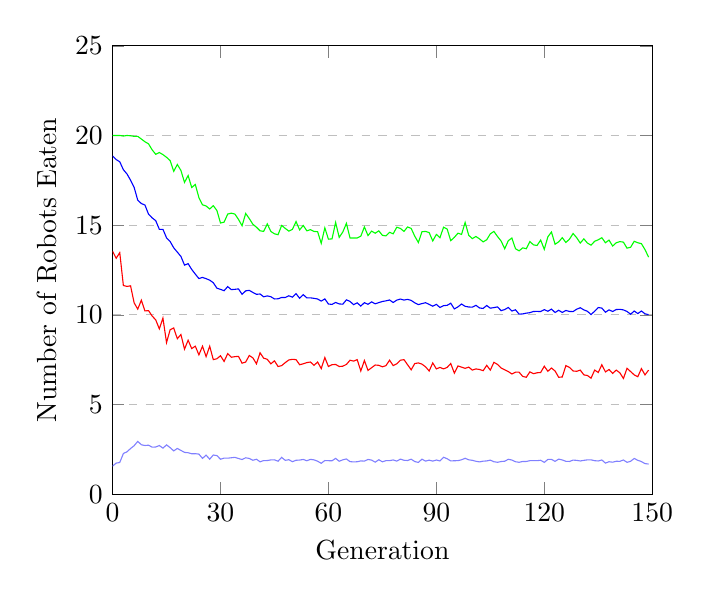
\begin{tikzpicture}
\begin{axis}[
	xlabel={Generation},
	ylabel={Number of Robots Eaten},
	xmin=0, xmax=150,
	ymin=0, ymax=25,
	xtick={0.0,30.0,60.0,90.0,120.0,150.0},
	ytick={0.0,5.0,10.0,15.0,20.0,25.0},
	ymajorgrids=true,
	grid style=dashed,
]

\addplot[
	color=green,
	]
	coordinates {
	(0,20.0)(1,20.0)(2,20.0)(3,19.96666666666667)(4,20.0)(5,19.983333333333334)(6,19.95)(7,19.95)(8,19.8)(9,19.65)(10,19.53333333333333)(11,19.200000000000003)(12,18.95)(13,19.05)(14,18.93333333333333)(15,18.78333333333333)(16,18.6)(17,18.0)(18,18.383333333333336)(19,18.05)(20,17.383333333333333)(21,17.766666666666662)(22,17.1)(23,17.266666666666666)(24,16.533333333333335)(25,16.133333333333336)(26,16.06666666666667)(27,15.899999999999999)(28,16.083333333333332)(29,15.816666666666668)(30,15.116666666666667)(31,15.16666666666667)(32,15.616666666666667)(33,15.666666666666666)(34,15.616666666666669)(35,15.316666666666666)(36,14.966666666666667)(37,15.650000000000002)(38,15.366666666666665)(39,15.049999999999999)(40,14.883333333333333)(41,14.683333333333332)(42,14.65)(43,15.066666666666665)(44,14.649999999999999)(45,14.516666666666667)(46,14.46666666666667)(47,14.983333333333333)(48,14.816666666666666)(49,14.666666666666666)(50,14.766666666666664)(51,15.2)(52,14.733333333333334)(53,14.983333333333334)(54,14.683333333333334)(55,14.750000000000004)(56,14.649999999999997)(57,14.633333333333335)(58,13.983333333333333)(59,14.850000000000003)(60,14.216666666666667)(61,14.233333333333336)(62,15.150000000000002)(63,14.316666666666665)(64,14.616666666666667)(65,15.100000000000001)(66,14.283333333333335)(67,14.283333333333335)(68,14.283333333333337)(69,14.383333333333331)(70,14.900000000000002)(71,14.416666666666664)(72,14.666666666666668)(73,14.55)(74,14.683333333333332)(75,14.433333333333332)(76,14.4)(77,14.6)(78,14.516666666666667)(79,14.883333333333335)(80,14.816666666666668)(81,14.65)(82,14.899999999999997)(83,14.816666666666666)(84,14.383333333333333)(85,14.033333333333335)(86,14.633333333333335)(87,14.65)(88,14.583333333333334)(89,14.116666666666667)(90,14.483333333333336)(91,14.3)(92,14.883333333333331)(93,14.783333333333333)(94,14.133333333333335)(95,14.316666666666665)(96,14.55)(97,14.483333333333333)(98,15.15)(99,14.433333333333334)(100,14.249999999999998)(101,14.366666666666667)(102,14.233333333333333)(103,14.066666666666666)(104,14.183333333333334)(105,14.516666666666666)(106,14.649999999999999)(107,14.366666666666669)(108,14.116666666666667)(109,13.683333333333332)(110,14.133333333333335)(111,14.283333333333335)(112,13.683333333333335)(113,13.566666666666663)(114,13.733333333333333)(115,13.683333333333334)(116,14.083333333333334)(117,13.900000000000002)(118,13.866666666666665)(119,14.16666666666667)(120,13.649999999999999)(121,14.35)(122,14.616666666666669)(123,13.933333333333335)(124,14.066666666666668)(125,14.299999999999997)(126,14.033333333333333)(127,14.216666666666667)(128,14.533333333333331)(129,14.299999999999999)(130,13.999999999999996)(131,14.233333333333334)(132,13.999999999999998)(133,13.883333333333333)(134,14.099999999999998)(135,14.183333333333332)(136,14.299999999999999)(137,14.016666666666667)(138,14.166666666666668)(139,13.833333333333334)(140,14.016666666666666)(141,14.083333333333332)(142,14.05)(143,13.716666666666669)(144,13.766666666666667)(145,14.100000000000001)(146,14.016666666666667)(147,13.966666666666669)(148,13.633333333333335)(149,13.216666666666665)
	};
\addplot[
	color=blue,
	]
	coordinates {
	(0,18.853472222222223)(1,18.655555555555555)(2,18.534027777777776)(3,18.091666666666665)(4,17.856250000000003)(5,17.50555555555556)(6,17.103472222222223)(7,16.391666666666666)(8,16.204166666666666)(9,16.12083333333333)(10,15.609027777777776)(11,15.405555555555553)(12,15.247916666666669)(13,14.767361111111114)(14,14.767361111111109)(15,14.291666666666668)(16,14.086805555555557)(17,13.73611111111111)(18,13.495138888888889)(19,13.255555555555553)(20,12.77152777777778)(21,12.851388888888888)(22,12.529166666666665)(23,12.269444444444446)(24,12.020138888888889)(25,12.085416666666667)(26,12.015277777777776)(27,11.93125)(28,11.787499999999998)(29,11.48263888888889)(30,11.42013888888889)(31,11.342361111111112)(32,11.573611111111111)(33,11.404166666666669)(34,11.420833333333334)(35,11.444444444444446)(36,11.14375)(37,11.335416666666665)(38,11.364583333333334)(39,11.246527777777777)(40,11.142361111111112)(41,11.160416666666668)(42,11.003472222222221)(43,11.054861111111109)(44,11.006944444444445)(45,10.883333333333335)(46,10.894444444444442)(47,10.964583333333334)(48,10.965972222222222)(49,11.05902777777778)(50,10.983333333333333)(51,11.17986111111111)(52,10.919444444444443)(53,11.124305555555557)(54,10.945833333333333)(55,10.946527777777776)(56,10.91736111111111)(57,10.880555555555555)(58,10.763888888888891)(59,10.886805555555554)(60,10.602083333333335)(61,10.580555555555556)(62,10.686805555555555)(63,10.606250000000003)(64,10.591666666666669)(65,10.834722222222222)(66,10.747916666666665)(67,10.563888888888886)(68,10.665972222222223)(69,10.487500000000002)(70,10.676388888888889)(71,10.586805555555555)(72,10.720833333333335)(73,10.613194444444444)(74,10.67986111111111)(75,10.742361111111112)(76,10.778472222222222)(77,10.826388888888891)(78,10.684722222222225)(79,10.818750000000001)(80,10.878472222222221)(81,10.82152777777778)(82,10.861111111111112)(83,10.803472222222224)(84,10.670138888888891)(85,10.56875)(86,10.625000000000002)(87,10.675694444444447)(88,10.581249999999999)(89,10.477777777777778)(90,10.581944444444446)(91,10.405555555555555)(92,10.511111111111113)(93,10.527083333333334)(94,10.645138888888889)(95,10.327083333333334)(96,10.441666666666666)(97,10.602083333333333)(98,10.472222222222223)(99,10.436111111111112)(100,10.426388888888889)(101,10.52986111111111)(102,10.381944444444443)(103,10.354166666666668)(104,10.519444444444444)(105,10.369444444444445)(106,10.400694444444444)(107,10.440277777777778)(108,10.231944444444446)(109,10.292361111111113)(110,10.409722222222225)(111,10.209722222222222)(112,10.280555555555557)(113,10.036111111111111)(114,10.048611111111109)(115,10.093055555555555)(116,10.118055555555555)(117,10.186805555555555)(118,10.187499999999998)(119,10.186111111111112)(120,10.288194444444445)(121,10.197916666666664)(122,10.31875)(123,10.12777777777778)(124,10.253472222222221)(125,10.129861111111111)(126,10.24236111111111)(127,10.186805555555555)(128,10.179166666666664)(129,10.310416666666667)(130,10.393749999999999)(131,10.275694444444445)(132,10.19375)(133,10.015277777777778)(134,10.2)(135,10.405555555555555)(136,10.375000000000002)(137,10.144444444444446)(138,10.273611111111112)(139,10.184027777777775)(140,10.293055555555554)(141,10.30486111111111)(142,10.27361111111111)(143,10.186805555555555)(144,10.032638888888886)(145,10.21111111111111)(146,10.068749999999998)(147,10.210416666666667)(148,10.05625)(149,10.008333333333331)
	};
\addplot[
	color=red,
	]
	coordinates {
	(0,13.550000000000002)(1,13.149999999999999)(2,13.466666666666665)(3,11.633333333333335)(4,11.583333333333334)(5,11.616666666666669)(6,10.666666666666666)(7,10.316666666666665)(8,10.816666666666666)(9,10.216666666666665)(10,10.233333333333334)(11,9.933333333333332)(12,9.716666666666665)(13,9.216666666666667)(14,9.816666666666665)(15,8.45)(16,9.166666666666666)(17,9.266666666666667)(18,8.666666666666666)(19,8.899999999999999)(20,8.083333333333334)(21,8.583333333333334)(22,8.116666666666667)(23,8.249999999999998)(24,7.7666666666666675)(25,8.25)(26,7.666666666666667)(27,8.25)(28,7.499999999999999)(29,7.55)(30,7.716666666666667)(31,7.3999999999999995)(32,7.833333333333334)(33,7.633333333333333)(34,7.666666666666667)(35,7.683333333333334)(36,7.300000000000001)(37,7.366666666666666)(38,7.733333333333334)(39,7.600000000000001)(40,7.266666666666666)(41,7.883333333333333)(42,7.583333333333333)(43,7.516666666666667)(44,7.2666666666666675)(45,7.433333333333333)(46,7.116666666666666)(47,7.166666666666668)(48,7.333333333333334)(49,7.483333333333335)(50,7.5166666666666675)(51,7.500000000000001)(52,7.216666666666665)(53,7.266666666666667)(54,7.333333333333335)(55,7.366666666666666)(56,7.1833333333333345)(57,7.366666666666668)(58,7.0)(59,7.616666666666668)(60,7.116666666666667)(61,7.216666666666667)(62,7.2333333333333325)(63,7.116666666666666)(64,7.133333333333334)(65,7.233333333333332)(66,7.466666666666666)(67,7.416666666666668)(68,7.500000000000001)(69,6.866666666666666)(70,7.45)(71,6.9)(72,7.050000000000001)(73,7.200000000000001)(74,7.183333333333334)(75,7.099999999999999)(76,7.166666666666666)(77,7.466666666666667)(78,7.166666666666668)(79,7.266666666666666)(80,7.466666666666667)(81,7.500000000000001)(82,7.216666666666666)(83,6.9333333333333345)(84,7.283333333333334)(85,7.316666666666667)(86,7.250000000000001)(87,7.100000000000001)(88,6.866666666666667)(89,7.316666666666667)(90,6.983333333333334)(91,7.0666666666666655)(92,6.9833333333333325)(93,7.066666666666666)(94,7.283333333333333)(95,6.749999999999999)(96,7.15)(97,7.083333333333333)(98,7.0166666666666675)(99,7.083333333333335)(100,6.916666666666665)(101,6.983333333333333)(102,6.950000000000002)(103,6.883333333333334)(104,7.183333333333334)(105,6.916666666666666)(106,7.3500000000000005)(107,7.233333333333333)(108,7.033333333333334)(109,6.933333333333334)(110,6.833333333333334)(111,6.7)(112,6.8)(113,6.800000000000001)(114,6.566666666666666)(115,6.516666666666666)(116,6.816666666666668)(117,6.716666666666668)(118,6.7666666666666675)(119,6.783333333333333)(120,7.133333333333333)(121,6.8500000000000005)(122,7.033333333333332)(123,6.866666666666667)(124,6.516666666666667)(125,6.533333333333333)(126,7.166666666666666)(127,7.066666666666666)(128,6.866666666666666)(129,6.8500000000000005)(130,6.916666666666666)(131,6.6499999999999995)(132,6.616666666666666)(133,6.466666666666668)(134,6.916666666666666)(135,6.783333333333333)(136,7.216666666666665)(137,6.816666666666666)(138,6.949999999999998)(139,6.7333333333333325)(140,6.916666666666667)(141,6.766666666666667)(142,6.450000000000001)(143,7.016666666666668)(144,6.833333333333333)(145,6.65)(146,6.549999999999999)(147,6.999999999999999)(148,6.6499999999999995)(149,6.916666666666667)
	};
\addplot[
	color=blue!50,
	]
	coordinates {
	(0,1.5626989059835774)(1,1.7292186330560189)(2,1.76606695128192)(3,2.2643119525582875)(4,2.360159661364281)(5,2.54218387052069)(6,2.7012325090253153)(7,2.942430845375984)(8,2.7535143177758736)(9,2.711521550178785)(10,2.730868257924848)(11,2.618196572804406)(12,2.6286009693255066)(13,2.710086656597167)(14,2.565642188752177)(15,2.746295290880908)(16,2.593024570370818)(17,2.4122341612564964)(18,2.5479061237730822)(19,2.4377224437858644)(20,2.3284380669283924)(21,2.309198388174861)(22,2.250387385306586)(23,2.2552187246199233)(24,2.233063432837089)(25,1.9932863045008986)(26,2.1740557501286077)(27,1.9490222640470698)(28,2.182287266951914)(29,2.1488093873031495)(30,1.9460209801689792)(31,2.0080232897855863)(32,2.0044670620154554)(33,2.028241023932433)(34,2.050666932726766)(35,1.9876328527482534)(36,1.9275955915796268)(37,2.0262365181227784)(38,1.9915412645531312)(39,1.889044939654505)(40,1.9457652884866066)(41,1.8019918669115649)(42,1.8701204033689227)(43,1.8727941584363526)(44,1.9086204770479602)(45,1.9140552514211528)(46,1.8358236394440979)(47,2.051085523390695)(48,1.8835865850319122)(49,1.920015204069164)(50,1.808808354595152)(51,1.8887071103567967)(52,1.8993619438348575)(53,1.93312547380359)(54,1.8622431238015997)(55,1.938868409615803)(56,1.9102151172459971)(57,1.8343151006540257)(58,1.7201464562812783)(59,1.8729554135362112)(60,1.865121484609783)(61,1.860479930455426)(62,1.99349335105667)(63,1.8335842472405208)(64,1.912778329407944)(65,1.9617522962076228)(66,1.8124362408514567)(67,1.7951824671251666)(68,1.8057508708583714)(69,1.852203321692268)(70,1.8414607500414955)(71,1.9341647523311494)(72,1.8981988116709463)(73,1.7836932810944366)(74,1.918195836839823)(75,1.8033720013833747)(76,1.8693403352812656)(77,1.869154613946461)(78,1.905151097657106)(79,1.8405094046972863)(80,1.951957536431071)(81,1.8875671423079967)(82,1.874991766698058)(83,1.9479102701252209)(84,1.8149710869070952)(85,1.7695203781980773)(86,1.9498921808215415)(87,1.8399640453133659)(88,1.8954419201471726)(89,1.8401691807509273)(90,1.9020000305850255)(91,1.850941567254191)(92,2.0572427585675808)(93,1.9740405596874222)(94,1.8520370466689169)(95,1.8614874683166576)(96,1.86856900321241)(97,1.9149679194783351)(98,1.9987634969596637)(99,1.9127475149267514)(100,1.886351724034577)(101,1.8315305904159245)(102,1.7979907977956748)(103,1.837974331390628)(104,1.8518144280049387)(105,1.896744736368088)(106,1.8071763492582928)(107,1.7753649967204186)(108,1.817701584177711)(109,1.8358451135188918)(110,1.9416256121494124)(111,1.90051651659138)(112,1.8064639160994072)(113,1.7756909557807228)(114,1.819880079077556)(115,1.8225223321592585)(116,1.864544848258108)(117,1.8651333858900803)(118,1.8665287365551189)(119,1.8876942497893996)(120,1.7705118817943866)(121,1.9349969880123676)(122,1.9384787454188661)(123,1.8275990593882077)(124,1.952406236043616)(125,1.9051796130975782)(126,1.8300764892212347)(127,1.821649717712897)(128,1.897674482084547)(129,1.8823812412266716)(130,1.8485734075811815)(131,1.883002623210848)(132,1.911625027733506)(133,1.9122822008996572)(134,1.8644421782012457)(135,1.8486859027874214)(136,1.9048126214042194)(137,1.7292826768411598)(138,1.8073494306277378)(139,1.7805203984002)(140,1.8325409995556543)(141,1.8288165009980633)(142,1.9053561424517498)(143,1.7723196250876052)(144,1.8328278590910208)(145,1.9898096767419478)(146,1.8858303250555464)(147,1.8156911632074872)(148,1.7003089073375903)(149,1.6785316547547298)
	};
\end{axis}
\end{tikzpicture}
}
		\caption{Some sample caption}
	\end{subfigure}%
}
\\
\\
\\
	\makebox[\linewidth][c]{%
	\begin{subfigure}[b]{0.7\textwidth}
		\centering
		\resizebox{0.9\linewidth}{!}{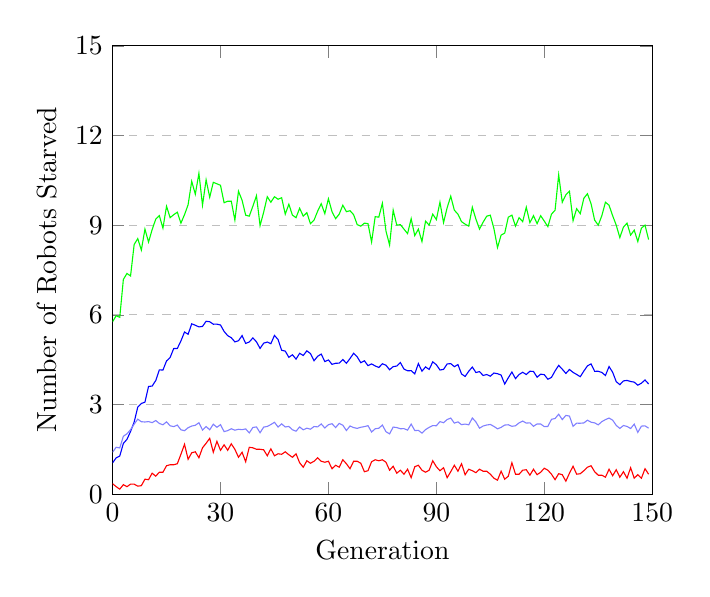
\begin{tikzpicture}
\begin{axis}[
	xlabel={Generation},
	ylabel={Number of Robots Starved},
	xmin=0, xmax=150,
	ymin=0, ymax=15,
	xtick={0.0,30.0,60.0,90.0,120.0,150.0},
	ytick={0.0,3.0,6.0,9.0,12.0,15.0},
	ymajorgrids=true,
	grid style=dashed,
]

\addplot[
	color=green,
	]
	coordinates {
	(0,5.766666666666667)(1,5.966666666666666)(2,5.916666666666666)(3,7.183333333333332)(4,7.383333333333333)(5,7.3)(6,8.350000000000001)(7,8.55)(8,8.166666666666668)(9,8.866666666666667)(10,8.433333333333334)(11,8.85)(12,9.2)(13,9.316666666666666)(14,8.9)(15,9.633333333333335)(16,9.25)(17,9.350000000000001)(18,9.433333333333334)(19,9.066666666666665)(20,9.35)(21,9.683333333333334)(22,10.466666666666665)(23,10.033333333333337)(24,10.733333333333334)(25,9.666666666666666)(26,10.516666666666666)(27,9.933333333333334)(28,10.433333333333335)(29,10.383333333333331)(30,10.333333333333334)(31,9.750000000000002)(32,9.8)(33,9.8)(34,9.166666666666666)(35,10.133333333333335)(36,9.833333333333334)(37,9.333333333333334)(38,9.299999999999999)(39,9.633333333333333)(40,9.983333333333333)(41,8.983333333333333)(42,9.433333333333332)(43,9.95)(44,9.766666666666667)(45,9.950000000000001)(46,9.866666666666669)(47,9.916666666666668)(48,9.366666666666665)(49,9.700000000000001)(50,9.333333333333332)(51,9.25)(52,9.566666666666666)(53,9.299999999999999)(54,9.416666666666666)(55,9.049999999999999)(56,9.166666666666664)(57,9.466666666666667)(58,9.716666666666667)(59,9.383333333333335)(60,9.883333333333335)(61,9.450000000000001)(62,9.216666666666665)(63,9.366666666666667)(64,9.666666666666666)(65,9.450000000000001)(66,9.483333333333334)(67,9.349999999999998)(68,9.016666666666666)(69,8.966666666666667)(70,9.066666666666668)(71,9.05)(72,8.433333333333332)(73,9.283333333333335)(74,9.266666666666666)(75,9.733333333333336)(76,8.799999999999999)(77,8.333333333333336)(78,9.500000000000002)(79,9.0)(80,9.01666666666667)(81,8.866666666666667)(82,8.716666666666667)(83,9.216666666666669)(84,8.65)(85,8.866666666666665)(86,8.450000000000001)(87,9.133333333333333)(88,9.0)(89,9.366666666666667)(90,9.183333333333334)(91,9.766666666666667)(92,9.083333333333332)(93,9.583333333333334)(94,9.966666666666667)(95,9.5)(96,9.366666666666665)(97,9.116666666666665)(98,9.033333333333333)(99,8.966666666666663)(100,9.6)(101,9.200000000000001)(102,8.866666666666665)(103,9.1)(104,9.299999999999999)(105,9.333333333333332)(106,8.883333333333333)(107,8.25)(108,8.666666666666668)(109,8.733333333333333)(110,9.266666666666666)(111,9.333333333333334)(112,8.966666666666667)(113,9.249999999999998)(114,9.116666666666667)(115,9.600000000000001)(116,9.083333333333334)(117,9.316666666666668)(118,9.049999999999999)(119,9.31666666666667)(120,9.133333333333333)(121,8.950000000000003)(122,9.366666666666667)(123,9.5)(124,10.683333333333334)(125,9.766666666666666)(126,10.016666666666666)(127,10.133333333333333)(128,9.15)(129,9.549999999999999)(130,9.383333333333333)(131,9.899999999999999)(132,10.049999999999999)(133,9.716666666666667)(134,9.166666666666668)(135,8.999999999999998)(136,9.316666666666665)(137,9.766666666666667)(138,9.666666666666668)(139,9.316666666666668)(140,9.0)(141,8.583333333333334)(142,8.933333333333332)(143,9.066666666666668)(144,8.666666666666664)(145,8.833333333333334)(146,8.45)(147,8.899999999999999)(148,9.000000000000002)(149,8.516666666666667)
	};
\addplot[
	color=blue,
	]
	coordinates {
	(0,1.0458333333333332)(1,1.2145833333333333)(2,1.2756944444444445)(3,1.6965277777777776)(4,1.8319444444444444)(5,2.0958333333333337)(6,2.4097222222222223)(7,2.909722222222222)(8,3.0333333333333337)(9,3.0777777777777784)(10,3.6027777777777783)(11,3.6152777777777776)(12,3.8)(13,4.158333333333334)(14,4.1506944444444445)(15,4.45486111111111)(16,4.570138888888889)(17,4.8708333333333345)(18,4.874305555555555)(19,5.125694444444445)(20,5.423611111111111)(21,5.349305555555555)(22,5.698611111111111)(23,5.650694444444444)(24,5.595138888888888)(25,5.611111111111112)(26,5.784027777777777)(27,5.7673611111111125)(28,5.685416666666668)(29,5.686805555555555)(30,5.659027777777777)(31,5.44375)(32,5.302083333333332)(33,5.232638888888889)(34,5.09375)(35,5.131944444444445)(36,5.304166666666667)(37,5.042361111111112)(38,5.090277777777777)(39,5.2270833333333355)(40,5.096527777777778)(41,4.875)(42,5.050694444444444)(43,5.088888888888889)(44,5.034027777777778)(45,5.309722222222222)(46,5.172916666666668)(47,4.813888888888888)(48,4.785416666666666)(49,4.576388888888888)(50,4.662499999999999)(51,4.5166666666666675)(52,4.711805555555556)(53,4.638888888888889)(54,4.79375)(55,4.703472222222221)(56,4.4625)(57,4.611805555555556)(58,4.686111111111111)(59,4.435416666666666)(60,4.489583333333333)(61,4.342361111111112)(62,4.377777777777778)(63,4.383333333333332)(64,4.503472222222222)(65,4.3784722222222205)(66,4.5368055555555555)(67,4.7118055555555545)(68,4.591666666666667)(69,4.395833333333333)(70,4.461805555555555)(71,4.299305555555557)(72,4.356249999999999)(73,4.288888888888889)(74,4.2375)(75,4.361805555555555)(76,4.312500000000001)(77,4.1618055555555555)(78,4.265972222222223)(79,4.284722222222221)(80,4.400694444444445)(81,4.1833333333333345)(82,4.128472222222222)(83,4.1305555555555555)(84,4.023611111111111)(85,4.36875)(86,4.113194444444444)(87,4.2555555555555555)(88,4.172222222222222)(89,4.425694444444444)(90,4.330555555555556)(91,4.152777777777778)(92,4.1729166666666675)(93,4.354861111111111)(94,4.367361111111111)(95,4.263888888888889)(96,4.334722222222222)(97,4.020138888888888)(98,3.9374999999999996)(99,4.1104166666666675)(100,4.252777777777778)(101,4.0680555555555555)(102,4.1000000000000005)(103,3.9701388888888887)(104,4.001388888888889)(105,3.946527777777777)(106,4.051388888888889)(107,4.028472222222223)(108,3.9840277777777784)(109,3.6840277777777777)(110,3.8930555555555557)(111,4.085416666666667)(112,3.8645833333333335)(113,4.003472222222222)(114,4.077083333333333)(115,4.001388888888888)(116,4.1125)(117,4.104166666666666)(118,3.913194444444444)(119,4.013194444444445)(120,3.9965277777777777)(121,3.842361111111111)(122,3.90625)(123,4.122222222222223)(124,4.3076388888888895)(125,4.179861111111111)(126,4.039583333333333)(127,4.170138888888889)(128,4.073611111111111)(129,4.003472222222221)(130,3.928472222222222)(131,4.118055555555555)(132,4.291666666666667)(133,4.3583333333333325)(134,4.1090277777777775)(135,4.110416666666666)(136,4.071527777777778)(137,3.96875)(138,4.26875)(139,4.0784722222222225)(140,3.7638888888888893)(141,3.6618055555555555)(142,3.788194444444445)(143,3.8048611111111117)(144,3.76875)(145,3.747222222222222)(146,3.644444444444445)(147,3.711805555555556)(148,3.8187499999999996)(149,3.686805555555555)
	};
\addplot[
	color=red,
	]
	coordinates {
	(0,0.35)(1,0.24999999999999997)(2,0.16666666666666666)(3,0.31666666666666665)(4,0.24999999999999997)(5,0.3333333333333333)(6,0.3333333333333333)(7,0.26666666666666666)(8,0.2833333333333333)(9,0.49999999999999994)(10,0.4833333333333333)(11,0.7)(12,0.6000000000000001)(13,0.7333333333333335)(14,0.7333333333333333)(15,0.9500000000000001)(16,0.9833333333333334)(17,0.9833333333333333)(18,1.0166666666666666)(19,1.3333333333333337)(20,1.666666666666667)(21,1.1666666666666667)(22,1.3833333333333335)(23,1.4166666666666667)(24,1.2166666666666666)(25,1.5499999999999998)(26,1.7000000000000004)(27,1.8666666666666667)(28,1.4000000000000001)(29,1.766666666666667)(30,1.466666666666667)(31,1.6500000000000004)(32,1.4666666666666668)(33,1.6833333333333331)(34,1.5)(35,1.2333333333333336)(36,1.4000000000000001)(37,1.0833333333333335)(38,1.5666666666666667)(39,1.5499999999999998)(40,1.5)(41,1.5)(42,1.4833333333333334)(43,1.2833333333333332)(44,1.5166666666666668)(45,1.2833333333333334)(46,1.3499999999999999)(47,1.3333333333333333)(48,1.4166666666666667)(49,1.3166666666666669)(50,1.2333333333333334)(51,1.35)(52,1.05)(53,0.9)(54,1.1166666666666667)(55,1.0333333333333334)(56,1.1)(57,1.2166666666666666)(58,1.0999999999999999)(59,1.0666666666666667)(60,1.0999999999999999)(61,0.85)(62,0.9666666666666668)(63,0.9)(64,1.1500000000000001)(65,1.0166666666666668)(66,0.8500000000000001)(67,1.1)(68,1.1)(69,1.0333333333333334)(70,0.75)(71,0.7833333333333333)(72,1.0833333333333335)(73,1.1500000000000001)(74,1.1166666666666667)(75,1.15)(76,1.0666666666666667)(77,0.8)(78,0.9333333333333333)(79,0.7000000000000001)(80,0.8)(81,0.6666666666666667)(82,0.8333333333333333)(83,0.55)(84,0.9166666666666666)(85,0.9666666666666666)(86,0.8000000000000002)(87,0.7333333333333333)(88,0.7999999999999999)(89,1.1166666666666667)(90,0.9166666666666667)(91,0.7833333333333333)(92,0.8833333333333334)(93,0.55)(94,0.75)(95,0.9666666666666666)(96,0.7666666666666666)(97,1.0166666666666666)(98,0.6499999999999999)(99,0.8333333333333334)(100,0.7833333333333333)(101,0.7166666666666667)(102,0.8333333333333335)(103,0.7666666666666666)(104,0.7666666666666667)(105,0.6666666666666667)(106,0.5333333333333333)(107,0.4666666666666666)(108,0.7666666666666666)(109,0.5)(110,0.6)(111,1.0500000000000003)(112,0.6666666666666666)(113,0.6666666666666666)(114,0.8)(115,0.8166666666666667)(116,0.6333333333333333)(117,0.8333333333333335)(118,0.65)(119,0.7333333333333333)(120,0.8666666666666668)(121,0.8000000000000002)(122,0.6666666666666666)(123,0.4833333333333333)(124,0.6833333333333332)(125,0.6499999999999999)(126,0.43333333333333335)(127,0.7)(128,0.9333333333333333)(129,0.6666666666666666)(130,0.6833333333333335)(131,0.7833333333333332)(132,0.9)(133,0.9500000000000001)(134,0.75)(135,0.6333333333333334)(136,0.6333333333333333)(137,0.5666666666666667)(138,0.8333333333333334)(139,0.6166666666666666)(140,0.8166666666666667)(141,0.5666666666666667)(142,0.75)(143,0.5333333333333333)(144,0.8833333333333334)(145,0.5333333333333333)(146,0.65)(147,0.5333333333333333)(148,0.8500000000000001)(149,0.6666666666666666)
	};
\addplot[
	color=blue!50,
	]
	coordinates {
	(0,1.4018656236185567)(1,1.5681300218111565)(2,1.5446603073709415)(3,1.9356676619553421)(4,2.019097201497308)(5,2.157835432654836)(6,2.339185215080197)(7,2.5077556813226933)(8,2.423208514610124)(9,2.4129459288342283)(10,2.427659471909309)(11,2.3910341558159915)(12,2.4629413391868074)(13,2.364527972525785)(14,2.3205289487566985)(15,2.417985603007099)(16,2.2867077015784387)(17,2.257610213818513)(18,2.310956437009541)(19,2.152615050348828)(20,2.1223248690372505)(21,2.2223903847846125)(22,2.277908865003934)(23,2.3040041084854717)(24,2.388505535407707)(25,2.144504107309114)(26,2.2617439296388118)(27,2.152962116183052)(28,2.339373565577375)(29,2.2361828085470097)(30,2.324026238512618)(31,2.0917230986253013)(32,2.1242320717186995)(33,2.1873478307542884)(34,2.138943049736312)(35,2.1689751417416594)(36,2.155990699963549)(37,2.1821486835944053)(38,2.0474985978308093)(39,2.229840913025318)(40,2.248889436311165)(41,2.0542980072927395)(42,2.242492815145739)(43,2.2640165658995532)(44,2.328392072652577)(45,2.404080343654768)(46,2.2451462002163325)(47,2.3504145822413176)(48,2.2468317962272453)(49,2.2650174348398293)(50,2.1542127975811827)(51,2.1063609007412976)(52,2.246859089016366)(53,2.1507404855112817)(54,2.208005322638693)(55,2.1715577508487347)(56,2.2616529536346412)(57,2.2498872841526825)(58,2.3472418760495315)(59,2.2132370160125925)(60,2.324202400010805)(61,2.355974244042933)(62,2.2264553127054065)(63,2.367012820335241)(64,2.3057845140398996)(65,2.127815892722732)(66,2.280403413934775)(67,2.2264633295324425)(68,2.1999973804981856)(69,2.2376004995504712)(70,2.25886261980979)(71,2.2906264551198072)(72,2.077373631684572)(73,2.1863685105593818)(74,2.2050130262737606)(75,2.3103242915444384)(76,2.087634912556033)(77,2.015552288414146)(78,2.2436551674307927)(79,2.2267229010968053)(80,2.1873798083414493)(81,2.1912188543376714)(82,2.142178106146297)(83,2.343427838997382)(84,2.1280116948516863)(85,2.13270463302169)(86,2.0430499452519695)(87,2.1590655592430066)(88,2.2340869619380355)(89,2.29379677883257)(90,2.2876332949050857)(91,2.426136245511977)(92,2.389393235677533)(93,2.4953740658417494)(94,2.5453352526905766)(95,2.3756273067238975)(96,2.417806117545828)(97,2.3235779079435654)(98,2.344219170587695)(99,2.3189280541854)(100,2.5472222071998836)(101,2.414755138324423)(102,2.206607613082537)(103,2.278527316318617)(104,2.312749155895062)(105,2.3310414310874523)(106,2.2665574277522467)(107,2.183677098546398)(108,2.233921480197757)(109,2.310695617802884)(110,2.3206975671440664)(111,2.268832779668199)(112,2.2872186894452726)(113,2.3845078707000305)(114,2.4449526167567917)(115,2.3765334297914906)(116,2.384983240821048)(117,2.269334262591855)(118,2.3482548164448644)(119,2.3463104423058407)(120,2.2592355210320925)(121,2.2645349001481376)(122,2.5030139590082077)(123,2.5299492361717117)(124,2.673873902442238)(125,2.4937801868260845)(126,2.634251662153934)(127,2.61117968314535)(128,2.268629050030047)(129,2.374160605228592)(130,2.3720036129868336)(131,2.3818343261332866)(132,2.474017494038653)(133,2.4069542565323183)(134,2.383506236235008)(135,2.3184923780232527)(136,2.425208576553106)(137,2.4930798736471678)(138,2.5447520775365216)(139,2.476154355523088)(140,2.2999046959678124)(141,2.198702000326418)(142,2.295588088591036)(143,2.2649730356637914)(144,2.1953749874239668)(145,2.3417906086484908)(146,2.0661488754944437)(147,2.2762918334467273)(148,2.284285747014353)(149,2.205796609342048)
	};
\end{axis}
\end{tikzpicture}
}
		\caption{Some sample caption}
	\end{subfigure}%
	\begin{subfigure}[b]{0.7\textwidth}
		\centering
		\resizebox{0.9\linewidth}{!}{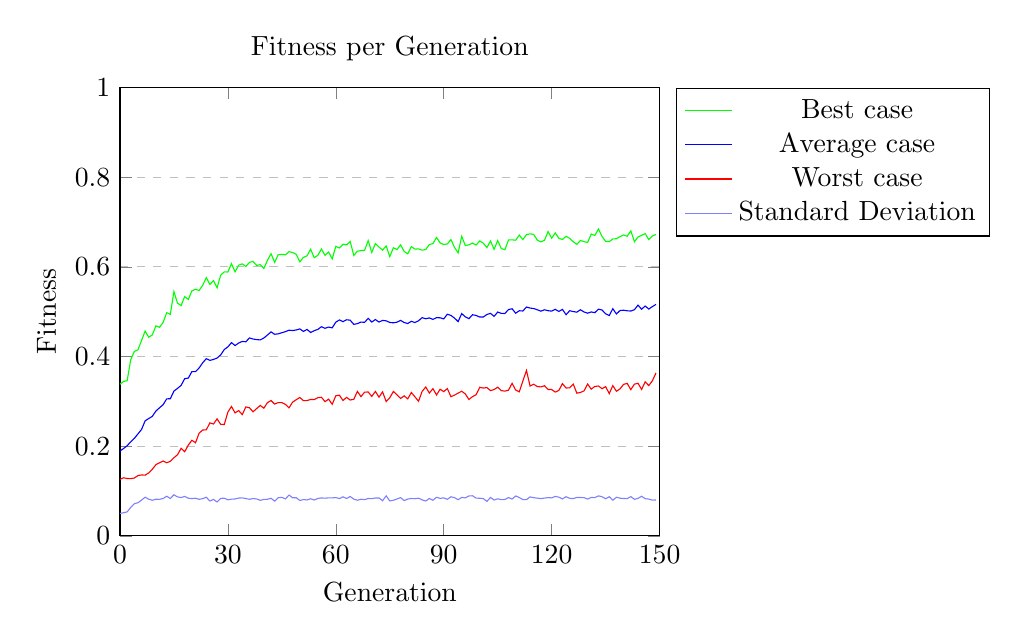
\begin{tikzpicture}
\begin{axis}[
	title={Fitness per Generation},
	xlabel={Generation},
	ylabel={Fitness},
	xmin=0, xmax=150,
	ymin=0, ymax=1,
	xtick={0.0,30.0,60.0,90.0,120.0,150.0},
	ytick={0.0,0.2,0.4,0.6000000000000001,0.8,1.0},
	legend pos=outer north east,
	ymajorgrids=true,
	grid style=dashed,
]

\addplot[
	color=green,
	]
	coordinates {
	(0,0.33821208333333336)(1,0.34445216666666656)(2,0.3461116666666667)(3,0.39306708333333334)(4,0.4112362500000001)(5,0.41507608333333335)(6,0.43569866666666657)(7,0.4569586666666666)(8,0.44307025000000005)(9,0.4483590833333333)(10,0.46860425000000006)(11,0.46526874999999995)(12,0.4762136666666667)(13,0.49801074999999995)(14,0.49405550000000004)(15,0.54479625)(16,0.5192201666666666)(17,0.5137533333333334)(18,0.5337270000000001)(19,0.5274525833333331)(20,0.5465690833333332)(21,0.5500465833333333)(22,0.5472538333333333)(23,0.55903925)(24,0.5761473333333333)(25,0.5607346666666666)(26,0.5696104166666667)(27,0.5532789999999999)(28,0.5815678333333334)(29,0.5889449166666666)(30,0.58856025)(31,0.6072923333333334)(32,0.5889329166666667)(33,0.6038636666666667)(34,0.6068265)(35,0.6009284166666666)(36,0.6101892499999999)(37,0.61208725)(38,0.6032037499999999)(39,0.605125)(40,0.5964690833333333)(41,0.6147515000000001)(42,0.6294088333333333)(43,0.6102600833333334)(44,0.62736975)(45,0.6278830833333333)(46,0.6269895833333333)(47,0.6338886666666667)(48,0.6320186666666666)(49,0.6280410000000001)(50,0.611443)(51,0.6210716666666667)(52,0.6246704166666667)(53,0.639408)(54,0.6205397500000001)(55,0.6257532499999999)(56,0.6397635)(57,0.6259579166666666)(58,0.6332144999999999)(59,0.6178640833333333)(60,0.6458751666666668)(61,0.6421617500000001)(62,0.6505223333333333)(63,0.6490993333333333)(64,0.6567665833333335)(65,0.6255482500000001)(66,0.6349291666666665)(67,0.6364199166666666)(68,0.6367249166666665)(69,0.6586703333333334)(70,0.632323)(71,0.6521987499999999)(72,0.6442244166666666)(73,0.6373845)(74,0.6466978333333332)(75,0.622744)(76,0.6427208333333334)(77,0.6386478333333333)(78,0.6491894166666669)(79,0.63458925)(80,0.6290991666666667)(81,0.6452242499999999)(82,0.6396554166666666)(83,0.6402380000000001)(84,0.6372920833333333)(85,0.6387872499999999)(86,0.6498334166666666)(87,0.6520078333333333)(88,0.6656728333333334)(89,0.6532835833333334)(90,0.6499644999999998)(91,0.65121925)(92,0.6609557500000001)(93,0.6432876666666667)(94,0.6312109166666666)(95,0.6681741666666666)(96,0.6474665833333334)(97,0.6492996666666667)(98,0.6530753333333332)(99,0.6486979166666665)(100,0.6578591666666667)(101,0.6527369166666667)(102,0.64318375)(103,0.657822)(104,0.6391198333333334)(105,0.6587069166666667)(106,0.6408390833333335)(107,0.63828775)(108,0.6600303333333334)(109,0.6603326666666667)(110,0.65950975)(111,0.6709094166666667)(112,0.6607955833333334)(113,0.671945)(114,0.6736861666666668)(115,0.6724033333333334)(116,0.6597614166666667)(117,0.6558213333333334)(118,0.6592628333333334)(119,0.6788443333333333)(120,0.66390975)(121,0.6758733333333334)(122,0.66356875)(123,0.6612043333333334)(124,0.6681244166666666)(125,0.6639570833333335)(126,0.6560470833333334)(127,0.6502261666666667)(128,0.6590324999999999)(129,0.6562537500000001)(130,0.6545598333333333)(131,0.6732358333333333)(132,0.6700824999999999)(133,0.6845232499999999)(134,0.6678613333333332)(135,0.6569171666666667)(136,0.6564796666666666)(137,0.6623675833333332)(138,0.6628160833333333)(139,0.6675004999999999)(140,0.6712509166666668)(141,0.6683513333333333)(142,0.6804799166666667)(143,0.6561523333333332)(144,0.6666870833333334)(145,0.6705645000000001)(146,0.6743001666666668)(147,0.6608083333333333)(148,0.6691263333333333)(149,0.6721471666666667)
	};
	\addlegendentry{Best case}
\addplot[
	color=blue,
	]
	coordinates {
	(0,0.1892287152777778)(1,0.19483818055555557)(2,0.20112732986111112)(3,0.2098738229166667)(4,0.2174859270833333)(5,0.22749311805555558)(6,0.23732014583333333)(7,0.2566508854166667)(8,0.2617790868055555)(9,0.26663142013888885)(10,0.27854202777777776)(11,0.28575993055555554)(12,0.2926342048611111)(13,0.30572268750000003)(14,0.3058464166666667)(15,0.3229007569444445)(16,0.32899188888888886)(17,0.3357292881944444)(18,0.3506692152777779)(19,0.3520097916666667)(20,0.3664764340277778)(21,0.36655724305555554)(22,0.37455701041666656)(23,0.38616544097222216)(24,0.39530508680555554)(25,0.39146511458333333)(26,0.3935624583333333)(27,0.39673564930555555)(28,0.4036460798611111)(29,0.41568923958333337)(30,0.42163724305555556)(31,0.4311035208333333)(32,0.42451403472222227)(33,0.43021594097222216)(34,0.43373331597222226)(35,0.43301769444444443)(36,0.4415907951388889)(37,0.4390995173611111)(38,0.4378402222222221)(39,0.4371244027777778)(40,0.4414401631944444)(41,0.44803172222222226)(42,0.45493828124999997)(43,0.44967493749999987)(44,0.4506916180555555)(45,0.45318057291666664)(46,0.45553301041666666)(47,0.4588158715277778)(48,0.4580353784722222)(49,0.4593361944444445)(50,0.46171434027777786)(51,0.45602521527777784)(52,0.4605252638888889)(53,0.45375914236111103)(54,0.4577638263888889)(55,0.46057010069444443)(56,0.46656746180555553)(57,0.4630025763888889)(58,0.46579630555555557)(59,0.4640651875000001)(60,0.4767023993055556)(61,0.48167377083333335)(62,0.4778751527777778)(63,0.48207191319444437)(64,0.4811827534722222)(65,0.4717859791666667)(66,0.47342753125)(67,0.47696311111111117)(68,0.4762609652777778)(69,0.48520590624999993)(70,0.4770281284722222)(71,0.4825983194444445)(72,0.47689825347222214)(73,0.48065988541666665)(74,0.47969986111111107)(75,0.4760745659722222)(76,0.4752752673611111)(77,0.4766931909722221)(78,0.4807497430555556)(79,0.4759674097222221)(80,0.4737414652777777)(81,0.47865392361111114)(82,0.4759579444444445)(83,0.4798090659722222)(84,0.4867818506944443)(85,0.4842753055555556)(86,0.4861788611111111)(87,0.4828941770833334)(88,0.48682276736111113)(89,0.4864383368055555)(90,0.48398461458333336)(91,0.49443302083333335)(92,0.4918032048611111)(93,0.48577570833333333)(94,0.4780102013888889)(95,0.4958281111111112)(96,0.48847686458333334)(97,0.48453817708333335)(98,0.4932769305555556)(99,0.49169409375)(100,0.4881403263888888)(101,0.4881840555555556)(102,0.4937906458333333)(103,0.49637465277777776)(104,0.4896843645833335)(105,0.4992675833333333)(106,0.496348)(107,0.4960439131944445)(108,0.5048510208333332)(109,0.5065911180555557)(110,0.49674099652777776)(111,0.5022184930555555)(112,0.5016035451388889)(113,0.5104500729166667)(114,0.5082066458333334)(115,0.5070799583333333)(116,0.5043865937500001)(117,0.5012411215277778)(118,0.5043043541666667)(119,0.5023484201388888)(120,0.5013423958333334)(121,0.5053585486111111)(122,0.5006361909722222)(123,0.5053148333333333)(124,0.49338186458333333)(125,0.5022063020833333)(126,0.5004022604166667)(127,0.49898881597222217)(128,0.5043969305555556)(129,0.49942461111111114)(130,0.4967070902777778)(131,0.49947651388888886)(132,0.4978773645833334)(133,0.5057595208333333)(134,0.5037602152777778)(135,0.49560496527777775)(136,0.49141657638888897)(137,0.5067845694444444)(138,0.49499797569444437)(139,0.5026517638888889)(140,0.5033374131944445)(141,0.502075236111111)(142,0.5015595868055556)(143,0.5044418159722223)(144,0.514744329861111)(145,0.50561115625)(146,0.5127208159722222)(147,0.5059389930555556)(148,0.5114030138888889)(149,0.5163874722222223)
	};
	\addlegendentry{Average case}
\addplot[
	color=red,
	]
	coordinates {
	(0,0.12611858333333334)(1,0.1296125)(2,0.12804633333333335)(3,0.12763616666666666)(4,0.12909083333333335)(5,0.13444791666666667)(6,0.13599433333333333)(7,0.13539383333333332)(8,0.14059316666666669)(9,0.14862058333333333)(10,0.15890141666666666)(11,0.16303224999999996)(12,0.16695483333333333)(13,0.16315441666666666)(14,0.1662314166666667)(15,0.17437875000000003)(16,0.1809853333333333)(17,0.1953740833333333)(18,0.18781841666666668)(19,0.20251041666666672)(20,0.21323808333333333)(21,0.2077201666666667)(22,0.22901725)(23,0.23617549999999998)(24,0.23652141666666665)(25,0.2522018333333333)(26,0.24957633333333337)(27,0.26102316666666664)(28,0.24872291666666668)(29,0.24850266666666662)(30,0.27616041666666663)(31,0.28853399999999996)(32,0.2743720833333334)(33,0.2795236666666666)(34,0.27056658333333333)(35,0.28777783333333334)(36,0.2858336666666667)(37,0.2767696666666667)(38,0.28406683333333327)(39,0.29096283333333334)(40,0.2848968333333334)(41,0.2972235833333334)(42,0.30189616666666663)(43,0.2939441666666666)(44,0.29738749999999997)(45,0.29740549999999993)(46,0.2932415833333334)(47,0.28561791666666664)(48,0.29845041666666666)(49,0.3037711666666667)(50,0.3087695)(51,0.3017048333333333)(52,0.301864)(53,0.30438616666666674)(54,0.3040012500000001)(55,0.30824549999999995)(56,0.30920291666666666)(57,0.29954441666666665)(58,0.30497225)(59,0.2935664166666667)(60,0.31250925)(61,0.3138300833333333)(62,0.30204575)(63,0.3089249166666667)(64,0.30306308333333337)(65,0.30464466666666673)(66,0.3223214166666667)(67,0.31068816666666665)(68,0.32057308333333334)(69,0.32104866666666665)(70,0.3110501666666667)(71,0.32234133333333337)(72,0.3094368333333333)(73,0.32116333333333336)(74,0.2996641666666667)(75,0.3080719166666666)(76,0.3222066666666666)(77,0.31483691666666663)(78,0.30646033333333333)(79,0.3123455833333333)(80,0.3056679166666667)(81,0.31993933333333335)(82,0.31012074999999995)(83,0.3003725833333333)(84,0.3224194166666667)(85,0.33205425)(86,0.31856208333333336)(87,0.32841624999999997)(88,0.31434608333333336)(89,0.32703575)(90,0.3218348333333334)(91,0.3286221666666667)(92,0.3105098333333334)(93,0.3139760833333333)(94,0.3185595)(95,0.32260925)(96,0.3166726666666666)(97,0.304295)(98,0.310602)(99,0.31480783333333334)(100,0.33142099999999997)(101,0.32968658333333334)(102,0.33087191666666665)(103,0.3240644166666667)(104,0.32640274999999996)(105,0.33165825)(106,0.3239715)(107,0.3228926666666666)(108,0.32495908333333334)(109,0.34029725000000005)(110,0.32527891666666664)(111,0.32135566666666665)(112,0.345783)(113,0.36888566666666667)(114,0.33416833333333334)(115,0.33829316666666664)(116,0.33318800000000004)(117,0.3323289166666667)(118,0.33496808333333333)(119,0.32652158333333337)(120,0.32644791666666667)(121,0.32070525)(122,0.3244545833333333)(123,0.3396974166666667)(124,0.32980450000000006)(125,0.3302770833333333)(126,0.33855874999999996)(127,0.31832408333333334)(128,0.31995366666666664)(129,0.3233975833333333)(130,0.3387651666666667)(131,0.3272289166666666)(132,0.33323591666666663)(133,0.33439824999999995)(134,0.32837849999999996)(135,0.3329693333333333)(136,0.31742908333333336)(137,0.33515)(138,0.32262425000000006)(139,0.3280254166666667)(140,0.3380020833333333)(141,0.3401444166666667)(142,0.3261596666666666)(143,0.3383919166666666)(144,0.34042116666666666)(145,0.32671875000000006)(146,0.34368174999999995)(147,0.3352318333333334)(148,0.3459923333333334)(149,0.3634994166666666)
	};
	\addlegendentry{Worst case}
\addplot[
	color=blue!50,
	]
	coordinates {
	(0,0.04990571018272887)(1,0.05164734027733858)(2,0.053546772670453956)(3,0.06347906361591148)(4,0.07175636469908404)(5,0.07398648693999497)(6,0.07988024506165646)(7,0.08623356273658832)(8,0.0819066084236592)(9,0.0793939198423555)(10,0.08173562541932398)(11,0.08150749505276376)(12,0.08341851260553493)(13,0.08851076299770222)(14,0.08337082549852891)(15,0.09162884610709995)(16,0.08703266290978717)(17,0.08538684854647163)(18,0.0881167394211968)(19,0.08402678835809113)(20,0.0832747475490794)(21,0.0839848954879026)(22,0.0815430962501775)(23,0.08303139487622224)(24,0.08628953032221219)(25,0.07769631156138633)(26,0.08139757271556407)(27,0.0756742990719409)(28,0.08362139824272598)(29,0.08413822755550751)(30,0.08040826115577623)(31,0.08190293454431316)(32,0.08235124380242051)(33,0.08441046577760628)(34,0.08477293758269122)(35,0.08320993953482314)(36,0.08172444992392487)(37,0.08328164013597082)(38,0.08239246431250863)(39,0.07926135716466405)(40,0.0813743734766287)(41,0.08162907819735707)(42,0.08390668711865913)(43,0.0775953117666094)(44,0.08512887733186407)(45,0.08602332987008154)(46,0.08243270689553421)(47,0.09104583905339132)(48,0.08499211093941492)(49,0.08514500442512976)(50,0.07900516892976615)(51,0.08107340697263093)(52,0.08016565201398886)(53,0.08289754277423962)(54,0.07987531015958231)(55,0.08350519089693059)(56,0.08468370936752384)(57,0.08406427134404856)(58,0.08488153743096717)(59,0.08474860178575078)(60,0.085477983778194)(61,0.0832797450649196)(62,0.08719230724529273)(63,0.08337542710516317)(64,0.08787407639259416)(65,0.0819978882340918)(66,0.07944318162267547)(67,0.08179128897684385)(68,0.08081266828636757)(69,0.083380584103269)(70,0.08305199374976656)(71,0.08452696671053998)(72,0.08456257454849105)(73,0.07837004738134276)(74,0.08936401454219096)(75,0.0780441242642561)(76,0.07950022928610233)(77,0.08230234617455526)(78,0.0854046716720918)(79,0.07870538056961252)(80,0.08219288861861966)(81,0.08336199361788335)(82,0.08292650421399175)(83,0.08413718748193713)(84,0.08026837884706366)(85,0.07774263815692495)(86,0.08346968195945742)(87,0.07953735402421565)(88,0.08614546983362724)(89,0.08359220892228333)(90,0.08487315477271397)(91,0.08156656173192534)(92,0.08725437631072955)(93,0.08527041272411584)(94,0.08064192884794012)(95,0.08587659105792854)(96,0.08469901804025476)(97,0.08910705428565904)(98,0.08948751091550468)(99,0.08427974109703978)(100,0.08396606779008814)(101,0.08321475436059203)(102,0.0769426351029836)(103,0.08571081807338216)(104,0.08000740344986643)(105,0.08264910096131858)(106,0.08093165643192503)(107,0.08112662001757835)(108,0.08560976568299966)(109,0.08213776301314915)(110,0.08915582689784185)(111,0.08552241742851242)(112,0.08088714669850526)(113,0.08084721660184138)(114,0.08698926116854118)(115,0.0852170580784423)(116,0.08414120684569965)(117,0.08322360522776164)(118,0.0843024002078371)(119,0.08531402931474877)(120,0.08480563778042598)(121,0.0881274158487641)(122,0.0863266905302829)(123,0.08254107247724997)(124,0.08740540936105647)(125,0.08387121414999173)(126,0.0831812147379376)(127,0.08581284935632937)(128,0.0855429930574323)(129,0.08537203292303416)(130,0.08215632685965885)(131,0.08580872596332167)(132,0.08528256199415953)(133,0.0892829857371216)(134,0.08732448796383828)(135,0.08282243848222282)(136,0.0873320035003628)(137,0.07969474394055442)(138,0.08613818064076141)(139,0.08409765552406931)(140,0.08340330291843617)(141,0.08313596041738082)(142,0.08768978171160918)(143,0.08162572536849841)(144,0.08364446902923474)(145,0.08835773663817009)(146,0.08304348804521583)(147,0.08206735890249883)(148,0.07973745732761475)(149,0.08023020884292173)
	};
	\addlegendentry{Standard Deviation}
\end{axis}
\end{tikzpicture}
}
		\caption{Some sample caption}
	\end{subfigure}%
}
\end{figure}

\newpage
\vspace*{-2.0cm}
\textbf{\Huge LARGE SAMPLE HEADER}
\vspace{1.5cm}
\begin{tikzpicture}[remember picture,overlay]
   \node[anchor=south east,inner sep=20pt] at (current page.south east)
              {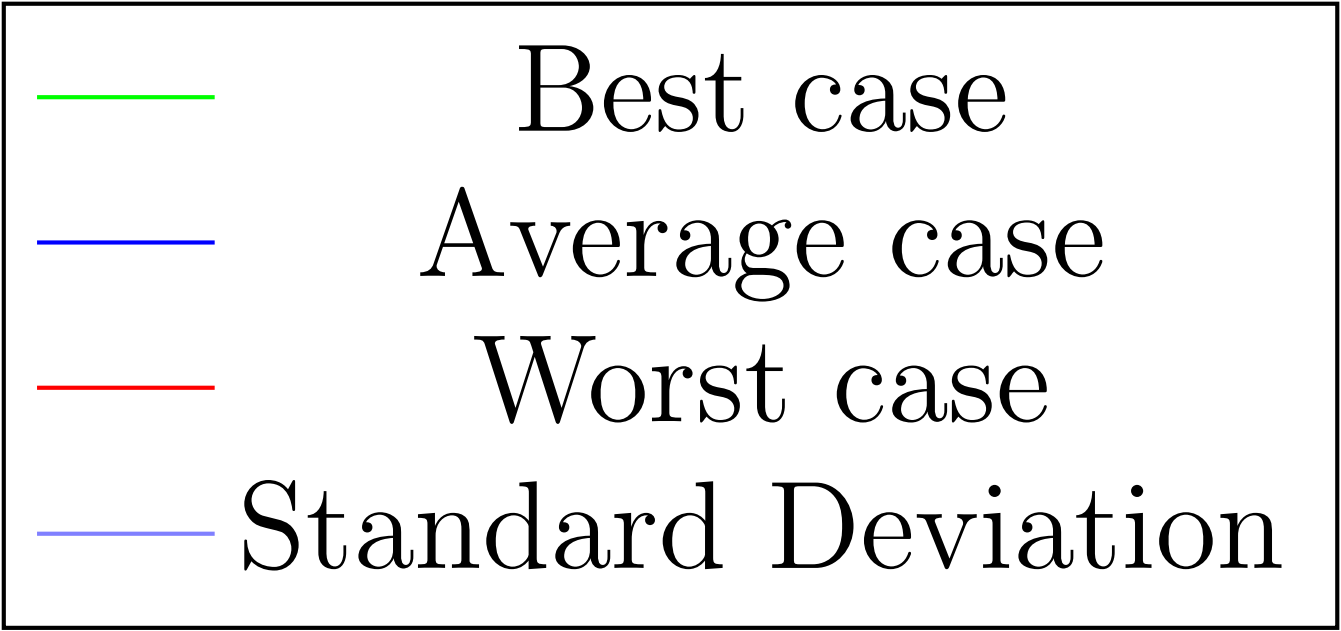
\includegraphics[scale=0.1]{chapters/res/generated_graph_legend.png}};
\end{tikzpicture}

\begin{figure}[H]
\vspace*{-1cm}
	\makebox[\linewidth][c]{%
	\begin{subfigure}[b]{0.7\textwidth}
		\centering
		\resizebox{0.9\linewidth}{!}{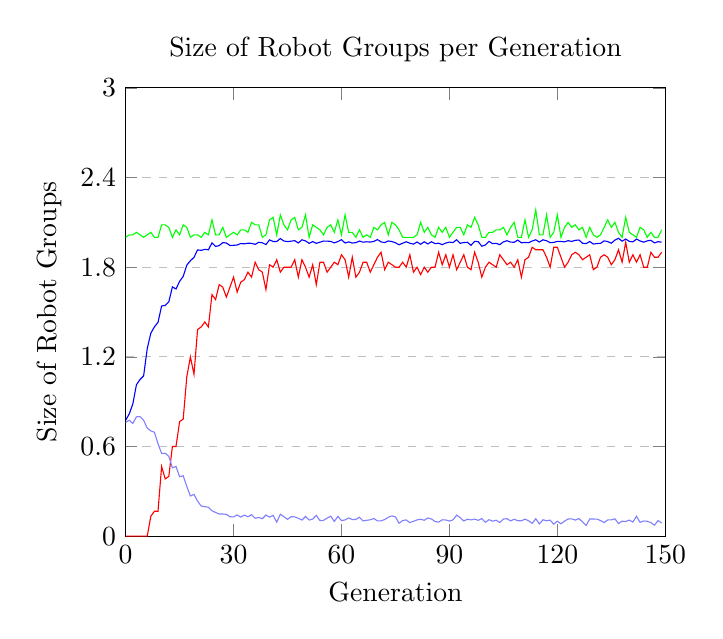
\begin{tikzpicture}
\begin{axis}[
	title={Size of Robot Groups per Generation},
	xlabel={Generation},
	ylabel={Size of Robot Groups},
	xmin=0, xmax=150,
	ymin=0, ymax=3,
	xtick={0.0,30.0,60.0,90.0,120.0,150.0},
	ytick={0.0,0.6,1.2,1.7999999999999998,2.4,3.0},
	ymajorgrids=true,
	grid style=dashed,
]

\addplot[
	color=green,
	]
	coordinates {
	(0,2.0000000000000004)(1,2.0166666666666675)(2,2.0166666666666675)(3,2.0333333333333337)(4,2.016666666666667)(5,2.0000000000000004)(6,2.016666666666667)(7,2.033333333333334)(8,2.0000000000000004)(9,2.0000000000000004)(10,2.083333333333334)(11,2.083333333333334)(12,2.0666666666666673)(13,2.0000000000000004)(14,2.0500000000000007)(15,2.016666666666667)(16,2.083333333333334)(17,2.066666666666667)(18,2.0000000000000004)(19,2.016666666666667)(20,2.0166666666666675)(21,2.0000000000000004)(22,2.0333333333333337)(23,2.0166666666666675)(24,2.1166666666666676)(25,2.016666666666667)(26,2.016666666666667)(27,2.0666666666666673)(28,2.0000000000000004)(29,2.016666666666667)(30,2.033333333333334)(31,2.0166666666666675)(32,2.0500000000000007)(33,2.0500000000000007)(34,2.033333333333334)(35,2.100000000000001)(36,2.0833333333333335)(37,2.083333333333334)(38,2.0000000000000004)(39,2.016666666666667)(40,2.116666666666667)(41,2.1333333333333337)(42,2.0166666666666675)(43,2.150000000000001)(44,2.083333333333334)(45,2.0500000000000007)(46,2.116666666666667)(47,2.1333333333333337)(48,2.0500000000000003)(49,2.066666666666667)(50,2.1500000000000004)(51,2.0000000000000004)(52,2.083333333333334)(53,2.0666666666666673)(54,2.0500000000000003)(55,2.016666666666667)(56,2.066666666666667)(57,2.083333333333334)(58,2.033333333333334)(59,2.116666666666667)(60,2.016666666666667)(61,2.150000000000001)(62,2.0333333333333337)(63,2.033333333333334)(64,2.0000000000000004)(65,2.0500000000000007)(66,2.0000000000000004)(67,2.016666666666667)(68,2.0000000000000004)(69,2.0666666666666673)(70,2.0500000000000003)(71,2.083333333333334)(72,2.1000000000000005)(73,2.016666666666667)(74,2.1)(75,2.0833333333333335)(76,2.0500000000000003)(77,2.0000000000000004)(78,2.0000000000000004)(79,2.0000000000000004)(80,2.0000000000000004)(81,2.016666666666667)(82,2.1000000000000005)(83,2.033333333333334)(84,2.066666666666667)(85,2.016666666666667)(86,2.0000000000000004)(87,2.0666666666666673)(88,2.0333333333333337)(89,2.0666666666666673)(90,2.0000000000000004)(91,2.0333333333333337)(92,2.066666666666667)(93,2.0666666666666673)(94,2.016666666666667)(95,2.083333333333334)(96,2.0666666666666673)(97,2.1333333333333337)(98,2.083333333333334)(99,2.0000000000000004)(100,2.0000000000000004)(101,2.033333333333334)(102,2.0333333333333337)(103,2.0500000000000007)(104,2.0500000000000007)(105,2.0666666666666673)(106,2.0166666666666675)(107,2.0666666666666673)(108,2.1000000000000005)(109,2.0000000000000004)(110,2.0000000000000004)(111,2.116666666666667)(112,2.0000000000000004)(113,2.0500000000000003)(114,2.183333333333334)(115,2.016666666666667)(116,2.016666666666667)(117,2.150000000000001)(118,2.0000000000000004)(119,2.0333333333333337)(120,2.150000000000001)(121,2.0000000000000004)(122,2.0666666666666673)(123,2.100000000000001)(124,2.0666666666666673)(125,2.083333333333334)(126,2.0500000000000007)(127,2.0666666666666673)(128,2.0000000000000004)(129,2.0666666666666673)(130,2.016666666666667)(131,2.0000000000000004)(132,2.0166666666666675)(133,2.0666666666666673)(134,2.116666666666667)(135,2.0666666666666673)(136,2.1000000000000005)(137,2.0333333333333337)(138,2.0000000000000004)(139,2.1333333333333337)(140,2.033333333333334)(141,2.0166666666666675)(142,2.0000000000000004)(143,2.0666666666666673)(144,2.0500000000000003)(145,2.0000000000000004)(146,2.033333333333334)(147,2.0000000000000004)(148,2.0000000000000004)(149,2.0500000000000007)
	};
\addplot[
	color=blue,
	]
	coordinates {
	(0,0.7756944444444444)(1,0.8180555555555556)(2,0.8847222222222223)(3,1.0131944444444443)(4,1.0486111111111112)(5,1.0729166666666665)(6,1.2548611111111112)(7,1.3583333333333334)(8,1.4006944444444445)(9,1.43125)(10,1.5402777777777776)(11,1.5444444444444445)(12,1.5680555555555558)(13,1.6680555555555552)(14,1.6541666666666666)(15,1.7055555555555555)(16,1.7381944444444444)(17,1.813888888888889)(18,1.843055555555556)(19,1.8659722222222224)(20,1.9159722222222226)(21,1.9125000000000003)(22,1.9194444444444447)(23,1.9166666666666672)(24,1.9625000000000004)(25,1.9388888888888893)(26,1.9444444444444446)(27,1.9645833333333336)(28,1.9618055555555556)(29,1.9451388888888894)(30,1.9465277777777779)(31,1.9486111111111115)(32,1.9583333333333337)(33,1.9562500000000003)(34,1.960416666666667)(35,1.9597222222222228)(36,1.9527777777777782)(37,1.966666666666667)(38,1.9631944444444445)(39,1.951388888888889)(40,1.982638888888889)(41,1.9722222222222225)(42,1.9715277777777782)(43,1.9916666666666671)(44,1.9750000000000008)(45,1.9715277777777782)(46,1.9743055555555558)(47,1.977777777777778)(48,1.961805555555556)(49,1.9833333333333334)(50,1.9763888888888892)(51,1.9597222222222226)(52,1.9715277777777782)(53,1.9597222222222228)(54,1.9673611111111118)(55,1.9750000000000003)(56,1.9743055555555558)(57,1.972916666666667)(58,1.9625000000000006)(59,1.9715277777777782)(60,1.9840277777777782)(61,1.961805555555556)(62,1.9694444444444448)(63,1.9618055555555562)(64,1.9645833333333336)(65,1.9750000000000003)(66,1.9673611111111116)(67,1.9701388888888893)(68,1.968055555555556)(69,1.972916666666667)(70,1.9847222222222227)(71,1.9694444444444448)(72,1.9645833333333338)(73,1.9756944444444444)(74,1.971527777777778)(75,1.9631944444444447)(76,1.9500000000000002)(77,1.960416666666667)(78,1.970138888888889)(79,1.9604166666666671)(80,1.954166666666667)(81,1.9687500000000004)(82,1.9534722222222225)(83,1.9701388888888893)(84,1.955555555555556)(85,1.9701388888888889)(86,1.9576388888888892)(87,1.9604166666666671)(88,1.9506944444444445)(89,1.9618055555555558)(90,1.9680555555555561)(91,1.9645833333333333)(92,1.984027777777778)(93,1.9597222222222224)(94,1.965277777777778)(95,1.966666666666667)(96,1.946527777777778)(97,1.9729166666666669)(98,1.9708333333333337)(99,1.9402777777777784)(100,1.9486111111111115)(101,1.972916666666667)(102,1.9576388888888894)(103,1.9597222222222228)(104,1.9506944444444447)(105,1.9694444444444446)(106,1.9770833333333335)(107,1.9680555555555561)(108,1.9666666666666668)(109,1.9812500000000002)(110,1.9631944444444447)(111,1.965277777777778)(112,1.963888888888889)(113,1.9750000000000003)(114,1.9833333333333336)(115,1.9680555555555561)(116,1.9833333333333334)(117,1.9770833333333337)(118,1.963888888888889)(119,1.9659722222222222)(120,1.9729166666666669)(121,1.9722222222222225)(122,1.9694444444444448)(123,1.9777777777777779)(124,1.9722222222222223)(125,1.979861111111111)(126,1.9819444444444447)(127,1.960416666666667)(128,1.9576388888888894)(129,1.9722222222222225)(130,1.9548611111111116)(131,1.9583333333333337)(132,1.9597222222222226)(133,1.9763888888888892)(134,1.971527777777778)(135,1.9604166666666667)(136,1.9812500000000002)(137,1.9937500000000001)(138,1.9743055555555558)(139,1.9881944444444448)(140,1.9729166666666667)(141,1.9694444444444446)(142,1.9881944444444446)(143,1.9756944444444446)(144,1.9673611111111113)(145,1.9763888888888892)(146,1.9798611111111115)(147,1.9625000000000001)(148,1.9708333333333334)(149,1.9673611111111113)
	};
\addplot[
	color=red,
	]
	coordinates {
	(0,0.0)(1,0.0)(2,0.0)(3,0.0)(4,0.0)(5,0.0)(6,0.0)(7,0.13333333333333333)(8,0.16666666666666666)(9,0.16666666666666669)(10,0.4666666666666667)(11,0.3833333333333333)(12,0.4)(13,0.6)(14,0.6)(15,0.7666666666666666)(16,0.7833333333333333)(17,1.0666666666666669)(18,1.2)(19,1.0833333333333333)(20,1.3833333333333335)(21,1.4000000000000001)(22,1.4333333333333338)(23,1.4000000000000001)(24,1.6166666666666671)(25,1.5833333333333337)(26,1.6833333333333336)(27,1.6666666666666667)(28,1.6000000000000003)(29,1.666666666666667)(30,1.7333333333333338)(31,1.6333333333333333)(32,1.7000000000000002)(33,1.716666666666667)(34,1.766666666666667)(35,1.7333333333333338)(36,1.8333333333333337)(37,1.7833333333333337)(38,1.766666666666667)(39,1.6500000000000004)(40,1.8166666666666669)(41,1.8000000000000003)(42,1.8500000000000003)(43,1.7666666666666668)(44,1.8000000000000005)(45,1.8000000000000003)(46,1.8000000000000003)(47,1.8500000000000003)(48,1.7333333333333338)(49,1.8500000000000003)(50,1.8000000000000005)(51,1.7333333333333336)(52,1.816666666666667)(53,1.6833333333333336)(54,1.8333333333333337)(55,1.8333333333333337)(56,1.7666666666666673)(57,1.8000000000000003)(58,1.8333333333333337)(59,1.816666666666667)(60,1.8833333333333337)(61,1.8500000000000005)(62,1.7333333333333336)(63,1.8666666666666671)(64,1.7333333333333338)(65,1.766666666666667)(66,1.833333333333334)(67,1.8333333333333337)(68,1.766666666666667)(69,1.816666666666667)(70,1.8666666666666671)(71,1.9000000000000006)(72,1.7833333333333339)(73,1.833333333333334)(74,1.8166666666666669)(75,1.8000000000000003)(76,1.8000000000000005)(77,1.8333333333333337)(78,1.8000000000000005)(79,1.8833333333333337)(80,1.766666666666667)(81,1.8000000000000005)(82,1.7500000000000002)(83,1.8000000000000003)(84,1.766666666666667)(85,1.8000000000000005)(86,1.8000000000000005)(87,1.9000000000000004)(88,1.816666666666667)(89,1.8833333333333337)(90,1.8000000000000005)(91,1.8833333333333335)(92,1.7833333333333337)(93,1.8333333333333335)(94,1.8833333333333337)(95,1.8000000000000005)(96,1.7833333333333337)(97,1.9000000000000004)(98,1.833333333333334)(99,1.7333333333333338)(100,1.8000000000000005)(101,1.833333333333334)(102,1.8166666666666669)(103,1.8000000000000005)(104,1.8833333333333337)(105,1.8500000000000005)(106,1.816666666666667)(107,1.8333333333333337)(108,1.8000000000000005)(109,1.8500000000000005)(110,1.7333333333333336)(111,1.8500000000000005)(112,1.8666666666666671)(113,1.933333333333334)(114,1.9166666666666672)(115,1.9166666666666672)(116,1.9166666666666672)(117,1.8666666666666674)(118,1.8000000000000005)(119,1.9333333333333338)(120,1.933333333333334)(121,1.8666666666666671)(122,1.8000000000000005)(123,1.8333333333333337)(124,1.883333333333334)(125,1.9000000000000006)(126,1.8833333333333337)(127,1.8500000000000005)(128,1.8666666666666671)(129,1.883333333333334)(130,1.7833333333333337)(131,1.8000000000000003)(132,1.8666666666666671)(133,1.883333333333334)(134,1.8666666666666674)(135,1.8166666666666673)(136,1.8500000000000003)(137,1.916666666666667)(138,1.8333333333333337)(139,1.9666666666666672)(140,1.833333333333334)(141,1.883333333333334)(142,1.833333333333334)(143,1.8833333333333337)(144,1.8000000000000005)(145,1.8000000000000003)(146,1.9000000000000006)(147,1.8666666666666671)(148,1.8666666666666671)(149,1.9000000000000006)
	};
\addplot[
	color=blue!50,
	]
	coordinates {
	(0,0.7614159090450933)(1,0.7757807491671067)(2,0.7544087555323536)(3,0.7988195058985315)(4,0.8004673382717862)(5,0.7753546021718657)(6,0.7235098976966002)(7,0.7047812658421969)(8,0.6957117412344618)(9,0.6190441273435283)(10,0.5537318012317776)(11,0.5548117083966644)(12,0.5343405880556895)(13,0.4570625229953232)(14,0.4668872486467571)(15,0.39774900071867436)(16,0.4047341409018805)(17,0.33340305431344874)(18,0.2689354892554084)(19,0.27971655974308673)(20,0.23449898062831126)(21,0.20170467423338997)(22,0.19800119472147765)(23,0.19342827848064031)(24,0.1702163714885154)(25,0.15879835620637958)(26,0.1483675419301849)(27,0.14861840928426734)(28,0.14605907495771642)(29,0.13012160389770056)(30,0.1292734706682764)(31,0.14177987302903589)(32,0.12795748608229998)(33,0.14095599961956004)(34,0.1299539986991229)(35,0.14413411273222498)(36,0.12027255290029112)(37,0.12529366364933622)(38,0.11724859555728279)(39,0.14158278613740435)(40,0.12756129441230915)(41,0.1392336094902727)(42,0.09412373051887182)(43,0.14657513903825764)(44,0.13003782428750216)(45,0.11306768276105157)(46,0.13058877163046415)(47,0.12933081265277485)(48,0.11973250991367042)(49,0.10796850583110702)(50,0.13200885820197944)(51,0.10788772831155787)(52,0.11439148972023228)(53,0.13954190293390098)(54,0.10447049810365501)(55,0.1060001199185803)(56,0.12093353056622914)(57,0.13402194230604864)(58,0.09861513863799841)(59,0.13289035499938143)(60,0.10438250510763122)(61,0.1091294675397513)(62,0.12217165492257268)(63,0.11102365308695276)(64,0.1120903738447784)(65,0.12666843990735804)(66,0.10208999795600011)(67,0.10649685163029914)(68,0.10969162220019557)(69,0.11849290575632164)(70,0.1020997177733918)(71,0.1027381349825486)(72,0.11123755326973189)(73,0.12647185643555395)(74,0.13610074248816414)(75,0.12892050228795418)(76,0.08625841504297121)(77,0.10482879740728407)(78,0.10882189382063215)(79,0.09111265537652499)(80,0.09981405632689963)(81,0.10888427531358842)(82,0.11352189618028377)(83,0.10650498664527486)(84,0.12211267911416544)(85,0.11512741252997753)(86,0.09839817392641365)(87,0.09404194277865398)(88,0.10967315034899221)(89,0.10855811853861437)(90,0.10129011206610888)(91,0.10896787493470816)(92,0.14116054767641145)(93,0.12402352787778814)(94,0.10154614818927575)(95,0.11357814118863291)(96,0.10880402598975845)(97,0.1144402707561652)(98,0.10615107260711795)(99,0.11783728026105911)(100,0.09287993267847548)(101,0.11049604189862557)(102,0.10036196437242878)(103,0.10682853281008854)(104,0.09129258464884069)(105,0.1148973181504892)(106,0.11706010970540617)(107,0.10218135418635763)(108,0.11351015069470566)(109,0.10356156729576324)(110,0.10289826510280457)(111,0.11413865912509777)(112,0.10288885888039406)(113,0.08585076067362954)(114,0.11684458528772004)(115,0.08204860517878944)(116,0.10963118763796313)(117,0.1036720574660969)(118,0.10725835393375083)(119,0.08049151027329221)(120,0.10048180048449286)(121,0.08281969089200361)(122,0.10120103624217376)(123,0.11505658636991868)(124,0.11611081850514067)(125,0.10745440993509583)(126,0.11813264197452775)(127,0.09560639698336977)(128,0.07184291875073169)(129,0.11516229840442618)(130,0.11485139238227793)(131,0.11442224872762179)(132,0.10444904792902525)(133,0.09094665221846868)(134,0.10906116483063259)(135,0.10950500172540203)(136,0.11609443799964818)(137,0.0848010032800147)(138,0.10040676781037741)(139,0.098111392524352)(140,0.10767994383201843)(141,0.09486442364416828)(142,0.13317652102979458)(143,0.09253402097200654)(144,0.1017360754102771)(145,0.09966817772248579)(146,0.09064238581703267)(147,0.07329465926625144)(148,0.1050945479282918)(149,0.08802219588681771)
	};
\end{axis}
\end{tikzpicture}
}
		\caption{Some sample caption}
	\end{subfigure}%
	\begin{subfigure}[b]{0.7\textwidth}
		\centering
		\resizebox{0.9\linewidth}{!}{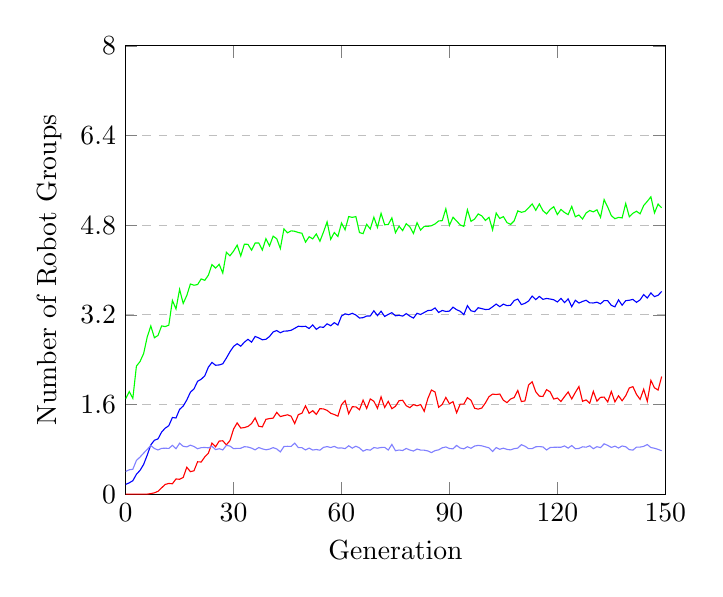
\begin{tikzpicture}
\begin{axis}[
	xlabel={Generation},
	ylabel={Number of Robot Groups},
	xmin=0, xmax=150,
	ymin=0, ymax=8,
	xtick={0.0,30.0,60.0,90.0,120.0,150.0},
	ytick={0.0,1.6,3.2,4.800000000000001,6.4,8.0},
	ymajorgrids=true,
	grid style=dashed,
]

\addplot[
	color=green,
	]
	coordinates {
	(0,1.7003333333333333)(1,1.83075)(2,1.7100833333333334)(3,2.2844999999999995)(4,2.366166666666667)(5,2.5076666666666667)(6,2.80425)(7,3.001166666666666)(8,2.7897499999999993)(9,2.83225)(10,3.0020833333333328)(11,2.989583333333333)(12,3.01525)(13,3.456583333333333)(14,3.3048333333333337)(15,3.65375)(16,3.4025000000000003)(17,3.545083333333333)(18,3.7502500000000003)(19,3.7279999999999998)(20,3.7397499999999995)(21,3.8403333333333336)(22,3.8155833333333335)(23,3.9065833333333333)(24,4.09675)(25,4.034333333333333)(26,4.100499999999999)(27,3.9451666666666663)(28,4.315416666666667)(29,4.253499999999999)(30,4.336166666666666)(31,4.4435833333333346)(32,4.250416666666666)(33,4.460666666666667)(34,4.457166666666667)(35,4.353583333333333)(36,4.4809166666666655)(37,4.481083333333334)(38,4.3565)(39,4.5584999999999996)(40,4.4303333333333335)(41,4.603750000000002)(42,4.557666666666666)(43,4.3838333333333335)(44,4.732)(45,4.662583333333333)(46,4.698333333333332)(47,4.690833333333333)(48,4.668666666666667)(49,4.655416666666666)(50,4.496666666666666)(51,4.593416666666667)(52,4.5553333333333335)(53,4.6425833333333335)(54,4.5120000000000005)(55,4.67775)(56,4.858583333333334)(57,4.547000000000001)(58,4.6690000000000005)(59,4.596583333333334)(60,4.838500000000001)(61,4.716916666666667)(62,4.952833333333333)(63,4.938666666666666)(64,4.9526666666666666)(65,4.667000000000001)(66,4.648416666666667)(67,4.814166666666667)(68,4.732499999999999)(69,4.941999999999999)(70,4.759083333333333)(71,5.011500000000001)(72,4.806583333333333)(73,4.811583333333333)(74,4.929749999999999)(75,4.6650833333333335)(76,4.780083333333333)(77,4.703083333333335)(78,4.826333333333334)(79,4.7692499999999995)(80,4.651833333333333)(81,4.841833333333334)(82,4.711833333333333)(83,4.778583333333334)(84,4.7781666666666665)(85,4.788666666666667)(86,4.821083333333334)(87,4.87475)(88,4.8799166666666665)(89,5.0918333333333345)(90,4.796166666666667)(91,4.9405833333333335)(92,4.874833333333332)(93,4.803333333333334)(94,4.777416666666666)(95,5.074583333333334)(96,4.867333333333334)(97,4.90875)(98,4.9994999999999985)(99,4.966166666666666)(100,4.8836666666666675)(101,4.9398333333333335)(102,4.715583333333335)(103,5.016000000000001)(104,4.919333333333334)(105,4.953166666666665)(106,4.845083333333334)(107,4.813083333333333)(108,4.877500000000001)(109,5.054333333333334)(110,5.0295)(111,5.044416666666667)(112,5.1089166666666666)(113,5.178916666666666)(114,5.0648333333333335)(115,5.178333333333334)(116,5.0566666666666675)(117,5.00075)(118,5.0795)(119,5.128833333333334)(120,4.989166666666667)(121,5.079666666666666)(122,5.02575)(123,4.988166666666666)(124,5.133916666666667)(125,4.949833333333333)(126,4.980833333333334)(127,4.9093333333333335)(128,5.0174166666666675)(129,5.061166666666667)(130,5.036833333333333)(131,5.073916666666666)(132,4.939916666666666)(133,5.254166666666666)(134,5.122416666666666)(135,4.97)(136,4.914750000000001)(137,4.93825)(138,4.928666666666666)(139,5.186916666666666)(140,4.950333333333334)(141,5.011166666666666)(142,5.047999999999999)(143,5.001333333333333)(144,5.15075)(145,5.22425)(146,5.305666666666665)(147,5.0183333333333335)(148,5.175416666666667)(149,5.109583333333333)
	};
\addplot[
	color=blue,
	]
	coordinates {
	(0,0.17362847222222225)(1,0.2017916666666667)(2,0.2392569444444444)(3,0.3544131944444444)(4,0.42396180555555546)(5,0.5304513888888891)(6,0.6960208333333333)(7,0.8799097222222222)(8,0.9613368055555555)(9,0.9858680555555559)(10,1.1072465277777777)(11,1.1775659722222223)(12,1.2213541666666667)(13,1.367267361111111)(14,1.3589270833333336)(15,1.5123784722222222)(16,1.5715138888888893)(17,1.6798784722222218)(18,1.818388888888889)(19,1.8782326388888886)(20,2.013916666666667)(21,2.050229166666667)(22,2.1112083333333334)(23,2.265979166666667)(24,2.350423611111111)(25,2.299614583333334)(26,2.305295138888889)(27,2.326159722222222)(28,2.42771875)(29,2.5405555555555557)(30,2.635322916666666)(31,2.683885416666667)(32,2.6397604166666664)(33,2.7105833333333327)(34,2.762947916666667)(35,2.712)(36,2.814013888888889)(37,2.7870520833333337)(38,2.7538020833333334)(39,2.763809027777778)(40,2.8131215277777772)(41,2.8936562500000003)(42,2.9190729166666665)(43,2.8794687499999996)(44,2.908996527777778)(45,2.9110520833333333)(46,2.923482638888889)(47,2.9587534722222224)(48,2.9959097222222217)(49,2.9902604166666666)(50,2.995364583333333)(51,2.9552152777777776)(52,3.018708333333333)(53,2.9408298611111103)(54,2.9845729166666666)(55,2.975607638888889)(56,3.039086805555556)(57,3.004760416666667)(58,3.059194444444444)(59,3.0164479166666665)(60,3.177625)(61,3.21742013888889)(62,3.20159375)(63,3.2265208333333337)(64,3.195979166666667)(65,3.142465277777777)(66,3.1489479166666667)(67,3.1779374999999996)(68,3.1796180555555553)(69,3.2719409722222212)(70,3.185413194444444)(71,3.264114583333334)(72,3.17059375)(73,3.2072118055555547)(74,3.2378506944444436)(75,3.1824340277777776)(76,3.1918055555555553)(77,3.1761701388888883)(78,3.2210659722222226)(79,3.1762118055555555)(80,3.1413819444444444)(81,3.2274409722222215)(82,3.2058229166666665)(83,3.2413090277777785)(84,3.2758263888888894)(85,3.281559027777778)(86,3.3227395833333326)(87,3.241538194444444)(88,3.2775034722222216)(89,3.2594826388888887)(90,3.2659097222222226)(91,3.336180555555556)(92,3.291243055555556)(93,3.2625520833333335)(94,3.2033333333333336)(95,3.3633263888888894)(96,3.2712881944444443)(97,3.255569444444444)(98,3.326246527777778)(99,3.309940972222222)(100,3.2942534722222225)(101,3.2985208333333333)(102,3.3424027777777776)(103,3.391899305555555)(104,3.3448020833333336)(105,3.390736111111111)(106,3.3636041666666667)(107,3.370152777777778)(108,3.4545486111111114)(109,3.480781249999999)(110,3.382430555555555)(111,3.404732638888889)(112,3.4457291666666667)(113,3.533729166666667)(114,3.470881944444444)(115,3.5279027777777783)(116,3.4752326388888894)(117,3.4919236111111114)(118,3.4818333333333333)(119,3.4684930555555553)(120,3.4294409722222228)(121,3.493666666666667)(122,3.4177986111111105)(123,3.4843125)(124,3.344368055555556)(125,3.45928125)(126,3.40984375)(127,3.4377708333333334)(128,3.4592569444444448)(129,3.412440972222222)(130,3.411284722222222)(131,3.424708333333333)(132,3.3950729166666664)(133,3.454190972222222)(134,3.451430555555556)(135,3.3686909722222227)(136,3.341878472222222)(137,3.467586805555556)(138,3.371357638888889)(139,3.4516111111111103)(140,3.4600625000000003)(141,3.47453125)(142,3.422513888888889)(143,3.467020833333333)(144,3.5606736111111115)(145,3.4996180555555556)(146,3.590607638888889)(147,3.5247222222222225)(148,3.5485069444444437)(149,3.616993055555555)
	};
\addplot[
	color=red,
	]
	coordinates {
	(0,0.0)(1,0.0)(2,0.0)(3,0.0)(4,0.0)(5,0.0)(6,0.0)(7,0.00975)(8,0.023166666666666672)(9,0.050916666666666666)(10,0.11258333333333334)(11,0.17250000000000001)(12,0.19124999999999998)(13,0.18466666666666667)(14,0.27066666666666667)(15,0.2649166666666667)(16,0.2975)(17,0.4804166666666666)(18,0.40083333333333326)(19,0.4168333333333333)(20,0.5771666666666667)(21,0.5731666666666666)(22,0.66425)(23,0.73)(24,0.9116666666666665)(25,0.8443333333333335)(26,0.9466666666666668)(27,0.9521666666666667)(28,0.879)(29,0.9554166666666667)(30,1.16125)(31,1.2714166666666666)(32,1.1789166666666666)(33,1.1881666666666666)(34,1.2076666666666667)(35,1.259)(36,1.3606666666666665)(37,1.2116666666666667)(38,1.1999999999999997)(39,1.3349166666666665)(40,1.3484166666666668)(41,1.3559999999999999)(42,1.458416666666667)(43,1.3845000000000003)(44,1.4005833333333333)(45,1.41625)(46,1.3898333333333335)(47,1.2600000000000002)(48,1.41875)(49,1.4435833333333334)(50,1.576583333333333)(51,1.4428333333333332)(52,1.4885833333333336)(53,1.4235000000000002)(54,1.5257499999999997)(55,1.52)(56,1.4953333333333332)(57,1.4430833333333337)(58,1.4204166666666667)(59,1.3914166666666663)(60,1.5964166666666662)(61,1.6676666666666666)(62,1.4345833333333329)(63,1.5590833333333334)(64,1.5574166666666667)(65,1.5056666666666667)(66,1.6777499999999999)(67,1.5280000000000002)(68,1.6987499999999998)(69,1.6569999999999998)(70,1.5305)(71,1.7359166666666668)(72,1.5465833333333334)(73,1.6556666666666666)(74,1.524416666666667)(75,1.5674166666666667)(76,1.6672499999999997)(77,1.6750833333333335)(78,1.5776666666666668)(79,1.5431666666666668)(80,1.5980833333333333)(81,1.576833333333333)(82,1.5984166666666668)(83,1.478333333333333)(84,1.7046666666666666)(85,1.8584166666666666)(86,1.8226666666666667)(87,1.55075)(88,1.5997500000000004)(89,1.7263333333333333)(90,1.6127500000000001)(91,1.6514166666666665)(92,1.4512499999999997)(93,1.6071666666666666)(94,1.6059999999999999)(95,1.7217500000000006)(96,1.67425)(97,1.5329166666666665)(98,1.5168333333333335)(99,1.536166666666667)(100,1.6270000000000002)(101,1.7399166666666668)(102,1.7845833333333334)(103,1.778333333333333)(104,1.786166666666667)(105,1.6755000000000002)(106,1.6325833333333333)(107,1.6968333333333332)(108,1.7235833333333337)(109,1.8504166666666668)(110,1.6525833333333335)(111,1.6633333333333336)(112,1.947833333333333)(113,2.0045)(114,1.8266666666666667)(115,1.7478333333333333)(116,1.7429999999999997)(117,1.864166666666667)(118,1.8246666666666669)(119,1.6971666666666667)(120,1.7139166666666668)(121,1.6538333333333333)(122,1.7404166666666665)(123,1.8227499999999999)(124,1.69875)(125,1.8151666666666668)(126,1.9196666666666669)(127,1.6565833333333337)(128,1.6812500000000001)(129,1.6223333333333332)(130,1.8341666666666665)(131,1.6590833333333335)(132,1.7268333333333328)(133,1.7320833333333334)(134,1.645)(135,1.83175)(136,1.6460000000000001)(137,1.7548333333333332)(138,1.6661666666666668)(139,1.7555)(140,1.894916666666667)(141,1.9181666666666666)(142,1.7788333333333337)(143,1.6914999999999996)(144,1.8712500000000003)(145,1.656)(146,2.0287499999999996)(147,1.8978333333333337)(148,1.857083333333333)(149,2.098333333333333)
	};
\addplot[
	color=blue!50,
	]
	coordinates {
	(0,0.4045690008403942)(1,0.4345146486627044)(2,0.444166164573904)(3,0.6009761638054792)(4,0.6618722960732871)(5,0.7318107932921486)(6,0.7985780216996883)(7,0.8681494947343847)(8,0.8140671011962864)(9,0.7881364947815761)(10,0.816563518526258)(11,0.8200845857892445)(12,0.8152825571738763)(13,0.8702997817082724)(14,0.8103412444288619)(15,0.9087619407943445)(16,0.8536291542022769)(17,0.8429751221252697)(18,0.8737075709595472)(19,0.8497571253700883)(20,0.8100796012977238)(21,0.8295793603126754)(22,0.8326252714803508)(23,0.8262324618884453)(24,0.8529690845960117)(25,0.7946717829315243)(26,0.8104466500861773)(27,0.7888584488298335)(28,0.8698049353655226)(29,0.857724924072532)(30,0.8116523735012899)(31,0.816311037554013)(32,0.8180902622190596)(33,0.8470669068442402)(34,0.8402979393522622)(35,0.8214232108654214)(36,0.7900117994227568)(37,0.8318515472230347)(38,0.8082469822459556)(39,0.7912389215882243)(40,0.8033610952012658)(41,0.8304760043472934)(42,0.8059887997593634)(43,0.7538232373925612)(44,0.8497678676981564)(45,0.853723826594109)(46,0.8516443929963067)(47,0.9094920365019241)(48,0.8304712929330302)(49,0.8289553404418285)(50,0.7880405137430435)(51,0.8213862333051506)(52,0.7866243021712621)(53,0.796300208769584)(54,0.7838647456133686)(55,0.8344733918178737)(56,0.8484596647027085)(57,0.8318947785151318)(58,0.8525373298520496)(59,0.8218812890039152)(60,0.8250310508117285)(61,0.8117652190625957)(62,0.8625652046718829)(63,0.8209951755505124)(64,0.8546600844157427)(65,0.8254475954963044)(66,0.7672392745487099)(67,0.7956094989389032)(68,0.7845671633204307)(69,0.8310696992446106)(70,0.8197533734782543)(71,0.8321054959856489)(72,0.8349058050208445)(73,0.786695806164151)(74,0.8869267893259394)(75,0.7751218425771522)(76,0.7868885449832498)(77,0.7786083744060956)(78,0.8150324028582048)(79,0.787095897806874)(80,0.7688901346476962)(81,0.8040857663854992)(82,0.7862979914992213)(83,0.7841835714863349)(84,0.7708105664405693)(85,0.74114907977197)(86,0.7763627914916612)(87,0.7899436105853218)(88,0.8263673700282745)(89,0.8421646520814321)(90,0.8140986333671826)(91,0.8076927950513129)(92,0.8692151730949196)(93,0.8226110849444372)(94,0.8078919170665151)(95,0.8455103628228873)(96,0.8181682537001236)(97,0.8582620721117569)(98,0.8697913917004374)(99,0.861953415878014)(100,0.843808565641803)(101,0.825873507884364)(102,0.7608019603522976)(103,0.8306060548314202)(104,0.8002495318860673)(105,0.8205269785508557)(106,0.7983373608720179)(107,0.7894017035026908)(108,0.8121201898097088)(109,0.8207108902987063)(110,0.8826309542138986)(111,0.8549735962214705)(112,0.8118611694195796)(113,0.8113161943364553)(114,0.8451956726073058)(115,0.8488785040198152)(116,0.8416632017231911)(117,0.7878229797050053)(118,0.8320294315820976)(119,0.8358529463161769)(120,0.8376593560127839)(121,0.836910008383062)(122,0.8595570411694577)(123,0.820960838729206)(124,0.86688295390923)(125,0.8105632921762453)(126,0.8148989190667776)(127,0.8445599326956814)(128,0.8377032979444511)(129,0.8628308214748689)(130,0.8105906674414362)(131,0.8467490557633096)(132,0.829345490288481)(133,0.8977253204045276)(134,0.8697669318607273)(135,0.8330988709550579)(136,0.855722599839588)(137,0.8229051677723618)(138,0.8598355588316887)(139,0.8451194024444071)(140,0.7936794751948583)(141,0.7859923073721408)(142,0.8391352475543208)(143,0.8394453446422161)(144,0.851851777783514)(145,0.8844172539046412)(146,0.8314099299783733)(147,0.8188119678271243)(148,0.7977757765149802)(149,0.7751389696747994)
	};
\end{axis}
\end{tikzpicture}
}
		\caption{Some sample caption}
	\end{subfigure}%
}
\\
\\
\\
\\
	\makebox[\linewidth][c]{%
	\begin{subfigure}[b]{0.7\textwidth}
		\centering
		\resizebox{0.9\linewidth}{!}{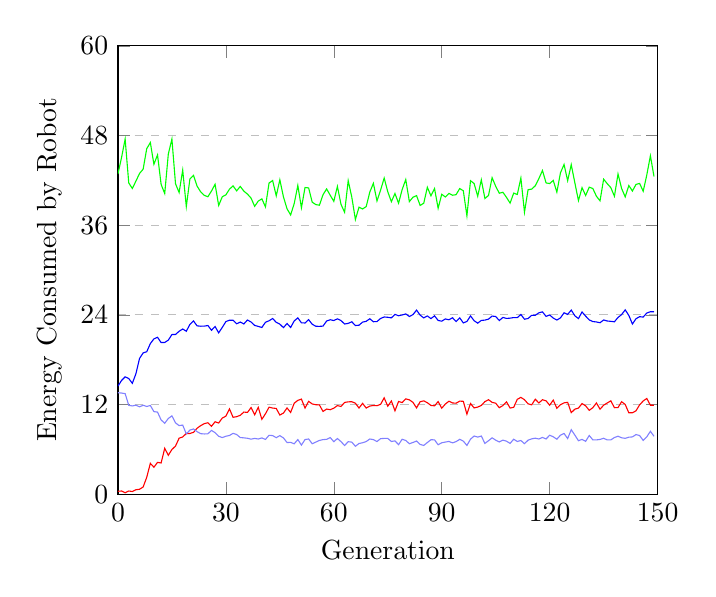
\begin{tikzpicture}
\begin{axis}[
	xlabel={Generation},
	ylabel={Energy Consumed by Robot},
	xmin=0, xmax=150,
	ymin=0, ymax=60,
	xtick={0.0,30.0,60.0,90.0,120.0,150.0},
	ytick={0.0,12.0,24.0,36.0,48.0,60.0},
	ymajorgrids=true,
	grid style=dashed,
]

\addplot[
	color=green,
	]
	coordinates {
	(0,42.85)(1,45.05)(2,47.516666666666666)(3,41.650000000000006)(4,40.9)(5,41.9)(6,42.916666666666664)(7,43.483333333333334)(8,46.23333333333334)(9,47.05)(10,44.15)(11,45.4)(12,41.45)(13,40.233333333333334)(14,45.51666666666667)(15,47.51666666666666)(16,41.533333333333346)(17,40.36666666666666)(18,43.36666666666666)(19,38.48333333333334)(20,42.18333333333333)(21,42.650000000000006)(22,41.21666666666666)(23,40.449999999999996)(24,39.983333333333334)(25,39.79999999999999)(26,40.56666666666666)(27,41.46666666666666)(28,38.633333333333326)(29,39.8)(30,40.05)(31,40.81666666666668)(32,41.25000000000001)(33,40.58333333333333)(34,41.18333333333333)(35,40.550000000000004)(36,40.15)(37,39.61666666666667)(38,38.516666666666666)(39,39.21666666666667)(40,39.51666666666667)(41,38.45000000000001)(42,41.633333333333326)(43,41.96666666666667)(44,39.91666666666666)(45,42.06666666666666)(46,39.78333333333333)(47,38.18333333333334)(48,37.366666666666674)(49,38.89999999999999)(50,41.31666666666668)(51,38.31666666666666)(52,41.033333333333324)(53,40.983333333333334)(54,39.066666666666684)(55,38.75)(56,38.666666666666664)(57,40.06666666666666)(58,40.849999999999994)(59,40.0)(60,39.18333333333334)(61,41.18333333333334)(62,38.78333333333333)(63,37.71666666666667)(64,41.94999999999999)(65,39.75000000000001)(66,36.75)(67,38.39999999999999)(68,38.16666666666668)(69,38.48333333333334)(70,40.416666666666664)(71,41.6)(72,39.23333333333333)(73,40.68333333333334)(74,42.3)(75,40.46666666666666)(76,39.13333333333334)(77,40.233333333333334)(78,38.93333333333333)(79,40.766666666666666)(80,42.1)(81,39.15)(82,39.73333333333333)(83,39.949999999999996)(84,38.63333333333333)(85,38.93333333333334)(86,41.06666666666666)(87,39.91666666666668)(88,40.89999999999999)(89,38.24999999999999)(90,40.13333333333333)(91,39.766666666666666)(92,40.25000000000001)(93,39.99999999999999)(94,40.08333333333333)(95,40.900000000000006)(96,40.6)(97,37.24999999999999)(98,41.95)(99,41.56666666666667)(100,39.866666666666674)(101,42.06666666666666)(102,39.566666666666656)(103,39.96666666666667)(104,42.35000000000001)(105,41.20000000000001)(106,40.26666666666667)(107,40.4)(108,39.71666666666667)(109,38.949999999999996)(110,40.28333333333333)(111,40.10000000000001)(112,42.30000000000001)(113,37.733333333333334)(114,40.75)(115,40.81666666666666)(116,41.26666666666667)(117,42.233333333333334)(118,43.31666666666667)(119,41.650000000000006)(120,41.566666666666656)(121,41.983333333333334)(122,40.41666666666668)(123,43.00000000000001)(124,44.116666666666674)(125,41.95)(126,44.1)(127,41.66666666666667)(128,39.28333333333333)(129,41.01666666666666)(130,39.96666666666667)(131,41.08333333333332)(132,40.900000000000006)(133,39.866666666666674)(134,39.25)(135,42.150000000000006)(136,41.550000000000004)(137,41.01666666666667)(138,39.86666666666667)(139,42.84999999999999)(140,40.89999999999999)(141,39.78333333333333)(142,41.3)(143,40.56666666666667)(144,41.45)(145,41.58333333333333)(146,40.53333333333333)(147,42.71666666666667)(148,45.28333333333334)(149,42.51666666666666)
	};
\addplot[
	color=blue,
	]
	coordinates {
	(0,14.450694444444446)(1,15.211805555555554)(2,15.69652777777778)(3,15.464583333333334)(4,14.825694444444444)(5,16.12152777777778)(6,18.15555555555555)(7,18.89722222222222)(8,19.052777777777777)(9,20.14097222222222)(10,20.779166666666665)(11,20.988194444444446)(12,20.28472222222222)(13,20.3)(14,20.608333333333334)(15,21.354861111111113)(16,21.369444444444444)(17,21.79375)(18,22.09861111111111)(19,21.799999999999997)(20,22.707638888888887)(21,23.17291666666667)(22,22.517361111111107)(23,22.47291666666667)(24,22.48125)(25,22.565972222222225)(26,21.931249999999995)(27,22.42361111111111)(28,21.583333333333336)(29,22.31180555555556)(30,23.090972222222224)(31,23.277777777777775)(32,23.265972222222228)(33,22.79861111111111)(34,23.024305555555554)(35,22.775000000000002)(36,23.306250000000002)(37,23.031250000000004)(38,22.580555555555552)(39,22.443749999999998)(40,22.303472222222222)(41,22.999999999999996)(42,23.199999999999996)(43,23.504166666666666)(44,22.9875)(45,22.748611111111114)(46,22.281944444444445)(47,22.82916666666667)(48,22.303472222222226)(49,23.185416666666665)(50,23.58680555555556)(51,22.925)(52,22.903472222222224)(53,23.351388888888888)(54,22.73333333333333)(55,22.46597222222222)(56,22.45347222222222)(57,22.48472222222222)(58,23.165277777777774)(59,23.336805555555557)(60,23.23194444444444)(61,23.459722222222226)(62,23.227083333333333)(63,22.76597222222222)(64,22.85138888888889)(65,23.06458333333333)(66,22.563194444444445)(67,22.605555555555554)(68,23.020138888888887)(69,23.128472222222225)(70,23.46736111111111)(71,23.074305555555554)(72,23.09166666666667)(73,23.509027777777774)(74,23.707638888888887)(75,23.66458333333333)(76,23.586805555555557)(77,24.054861111111116)(78,23.872222222222224)(79,23.974999999999998)(80,24.116666666666664)(81,23.772222222222222)(82,24.02222222222222)(83,24.627083333333335)(84,23.952777777777776)(85,23.58333333333333)(86,23.849305555555553)(87,23.49027777777778)(88,23.85763888888889)(89,23.243750000000002)(90,23.146527777777774)(91,23.444444444444443)(92,23.334722222222226)(93,23.601388888888888)(94,23.09236111111111)(95,23.59375)(96,22.91111111111111)(97,23.110416666666673)(98,23.84791666666667)(99,23.21388888888888)(100,22.880555555555556)(101,23.247222222222224)(102,23.288888888888895)(103,23.41944444444444)(104,23.83125)(105,23.768055555555556)(106,23.231944444444444)(107,23.645138888888894)(108,23.51527777777778)(109,23.547916666666666)(110,23.629861111111115)(111,23.616666666666667)(112,24.04375)(113,23.41111111111111)(114,23.500000000000004)(115,23.92986111111111)(116,23.93541666666667)(117,24.263888888888886)(118,24.392361111111114)(119,23.78888888888889)(120,23.975)(121,23.561805555555555)(122,23.29444444444445)(123,23.5875)(124,24.269444444444442)(125,24.05347222222223)(126,24.63194444444444)(127,23.865277777777777)(128,23.493055555555557)(129,24.381249999999998)(130,23.820138888888888)(131,23.31527777777778)(132,23.094444444444445)(133,23.041666666666668)(134,22.936805555555555)(135,23.307638888888892)(136,23.170833333333334)(137,23.122916666666672)(138,23.065277777777776)(139,23.643749999999997)(140,24.032638888888886)(141,24.659722222222218)(142,23.919444444444444)(143,22.766666666666662)(144,23.47222222222222)(145,23.750000000000004)(146,23.691666666666674)(147,24.238888888888887)(148,24.40625)(149,24.40069444444445)
	};
\addplot[
	color=red,
	]
	coordinates {
	(0,0.3833333333333333)(1,0.41666666666666663)(2,0.18333333333333332)(3,0.41666666666666663)(4,0.35)(5,0.5833333333333333)(6,0.6499999999999999)(7,0.9500000000000001)(8,2.25)(9,4.116666666666666)(10,3.5999999999999996)(11,4.25)(12,4.166666666666665)(13,6.133333333333333)(14,5.2)(15,5.966666666666665)(16,6.433333333333334)(17,7.4833333333333325)(18,7.6499999999999995)(19,8.116666666666665)(20,8.116666666666667)(21,8.266666666666667)(22,8.816666666666665)(23,9.166666666666666)(24,9.433333333333334)(25,9.549999999999999)(26,9.083333333333334)(27,9.683333333333332)(28,9.516666666666666)(29,10.183333333333332)(30,10.433333333333332)(31,11.4)(32,10.283333333333335)(33,10.366666666666667)(34,10.55)(35,10.983333333333334)(36,10.933333333333334)(37,11.583333333333336)(38,10.616666666666667)(39,11.616666666666667)(40,10.016666666666667)(41,10.75)(42,11.633333333333333)(43,11.516666666666667)(44,11.466666666666669)(45,10.583333333333334)(46,10.849999999999998)(47,11.533333333333333)(48,10.933333333333334)(49,12.166666666666666)(50,12.55)(51,12.716666666666665)(52,11.516666666666664)(53,12.416666666666666)(54,12.066666666666668)(55,11.966666666666667)(56,11.933333333333335)(57,11.066666666666665)(58,11.383333333333335)(59,11.299999999999999)(60,11.500000000000002)(61,11.85)(62,11.73333333333333)(63,12.266666666666667)(64,12.350000000000001)(65,12.366666666666665)(66,12.166666666666666)(67,11.516666666666667)(68,12.15)(69,11.516666666666666)(70,11.783333333333333)(71,11.866666666666669)(72,11.833333333333332)(73,12.01666666666667)(74,12.883333333333335)(75,11.766666666666667)(76,12.466666666666665)(77,11.150000000000002)(78,12.4)(79,12.25)(80,12.75)(81,12.616666666666667)(82,12.283333333333333)(83,11.533333333333331)(84,12.366666666666667)(85,12.483333333333334)(86,12.233333333333333)(87,11.866666666666665)(88,11.816666666666666)(89,12.383333333333335)(90,11.5)(91,12.049999999999997)(92,12.433333333333332)(93,12.2)(94,12.166666666666664)(95,12.45)(96,12.416666666666666)(97,10.7)(98,12.133333333333335)(99,11.533333333333333)(100,11.65)(101,11.866666666666667)(102,12.383333333333335)(103,12.633333333333331)(104,12.283333333333335)(105,12.166666666666666)(106,11.566666666666665)(107,11.85)(108,12.35)(109,11.516666666666666)(110,11.616666666666667)(111,12.683333333333334)(112,12.95)(113,12.633333333333333)(114,12.08333333333333)(115,11.950000000000001)(116,12.699999999999998)(117,12.200000000000001)(118,12.633333333333335)(119,12.483333333333333)(120,11.9)(121,12.583333333333332)(122,11.483333333333334)(123,11.966666666666665)(124,12.216666666666669)(125,12.283333333333337)(126,10.900000000000002)(127,11.366666666666665)(128,11.516666666666664)(129,12.116666666666667)(130,11.816666666666666)(131,11.216666666666669)(132,11.566666666666665)(133,12.200000000000001)(134,11.366666666666665)(135,11.9)(136,12.200000000000001)(137,12.483333333333333)(138,11.566666666666668)(139,11.583333333333334)(140,12.366666666666667)(141,11.999999999999996)(142,10.883333333333333)(143,10.883333333333333)(144,11.150000000000002)(145,11.950000000000001)(146,12.466666666666669)(147,12.800000000000002)(148,11.899999999999999)(149,11.9)
	};
\addplot[
	color=blue!50,
	]
	coordinates {
	(0,13.568087900390331)(1,13.528715234600082)(2,13.44672548257456)(3,11.882215701741497)(4,11.800512548890454)(5,11.902793017659214)(6,11.680015832063678)(7,11.891820900965104)(8,11.728652416088732)(9,11.861577131656794)(10,11.039589098866342)(11,10.980379170882252)(12,9.923872617170634)(13,9.484580358384187)(14,10.12218441181483)(15,10.474828704788766)(16,9.535492939723103)(17,9.170498313207414)(18,9.237827367503117)(19,8.0611329553564)(20,8.569835974775499)(21,8.718157118463933)(22,8.358065050988191)(23,8.091769061214984)(24,8.050688129664113)(25,8.07326636146528)(26,8.526651969881247)(27,8.225034588153994)(28,7.7446683220000665)(29,7.567967342064696)(30,7.743356944163276)(31,7.850480532483825)(32,8.132310714603063)(33,7.9735810224708406)(34,7.5714396920827)(35,7.531429362936355)(36,7.476692983796327)(37,7.354348915825212)(38,7.458660487452465)(39,7.374483108244286)(40,7.522912185323269)(41,7.31812729577751)(42,7.872828368614227)(43,7.831743513020669)(44,7.553593578150492)(45,7.827962481041477)(46,7.520954107215257)(47,6.904749402162643)(48,6.923141131249509)(49,6.7349448813319945)(50,7.3053470437945345)(51,6.563438525655783)(52,7.301779106811725)(53,7.378594539674514)(54,6.743906885716656)(55,6.9643062801073645)(56,7.184642678582021)(57,7.294856842132462)(58,7.330269001156066)(59,7.572715022464537)(60,7.016828808142398)(61,7.441535909922057)(62,7.022151126369867)(63,6.507825311450545)(64,7.0137686885035935)(65,6.9631524594794945)(66,6.4030611112529305)(67,6.774371285519779)(68,6.874411748189702)(69,7.038313595983277)(70,7.375165920307198)(71,7.297659214174119)(72,7.0347972472870195)(73,7.423443076397365)(74,7.456768797931699)(75,7.453866151779209)(76,7.045407186086702)(77,7.12508196465002)(78,6.619647988124534)(79,7.34345355279325)(80,7.1844949142700205)(81,6.743051448119919)(82,6.90966338040585)(83,7.1006724831919446)(84,6.651137817407766)(85,6.51577084500029)(86,6.906350980174475)(87,7.278678258670067)(88,7.262882780868531)(89,6.60637847171212)(90,6.872920099916377)(91,6.966865375401991)(92,7.050477023181985)(93,6.8595778592346655)(94,7.030624792948466)(95,7.329535144859221)(96,7.088151916602351)(97,6.518360426495708)(98,7.3559142878206245)(99,7.774911104652688)(100,7.630890158835392)(101,7.776219885566691)(102,6.7835513364236135)(103,7.1474654759555785)(104,7.533403721874176)(105,7.219771827574244)(106,6.984236044777888)(107,7.22905292918719)(108,7.083825239157489)(109,6.787069861141458)(110,7.348271634954806)(111,7.043257005684202)(112,7.1802350989065)(113,6.747041919250776)(114,7.2219258948287495)(115,7.396119680061793)(116,7.485950814964774)(117,7.37793084389116)(118,7.587246778824361)(119,7.3789294112900565)(120,7.880020632694641)(121,7.674771498397564)(122,7.34811855510635)(123,7.88544564592819)(124,8.118739204194087)(125,7.433855965112449)(126,8.624820397338885)(127,7.901745824013726)(128,7.146633414288165)(129,7.3270233108150045)(130,7.063611325765004)(131,7.848917471029941)(132,7.261426172232906)(133,7.2537304862789584)(134,7.32162974736117)(135,7.473482734787646)(136,7.256361520654363)(137,7.252841999651676)(138,7.573809940471945)(139,7.746751811361144)(140,7.541789574763703)(141,7.466159986505602)(142,7.616315184040483)(143,7.656949683564131)(144,7.968884822510555)(145,7.840851961956279)(146,7.183242911226776)(147,7.6667994152673415)(148,8.40926717222846)(149,7.741644535051923)
	};
\end{axis}
\end{tikzpicture}
}
		\caption{Some sample caption}
	\end{subfigure}%
	\begin{subfigure}[b]{0.7\textwidth}
		\centering
		\resizebox{0.9\linewidth}{!}{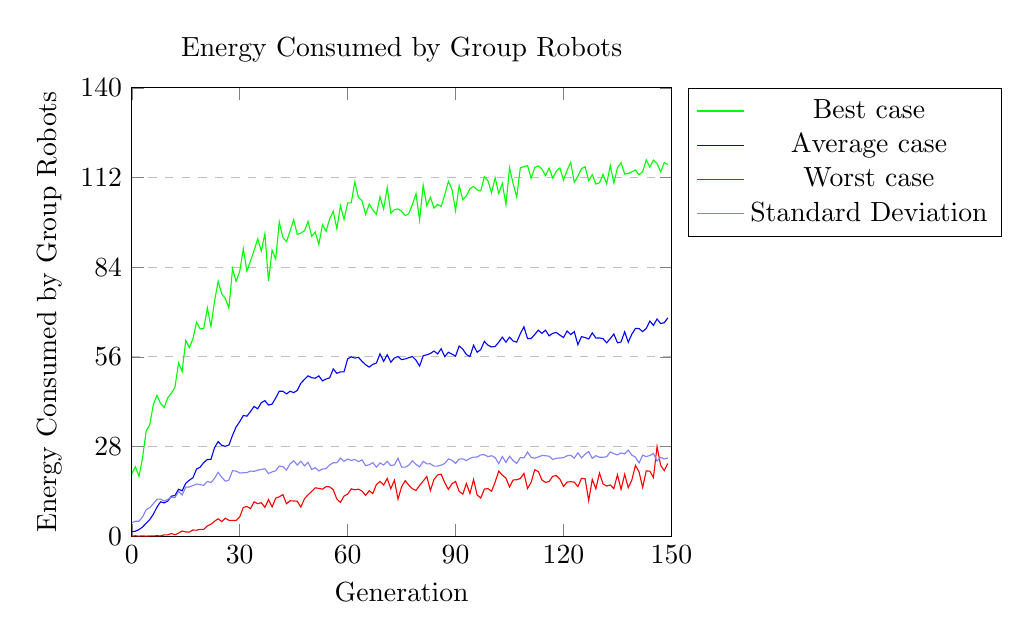
\begin{tikzpicture}
\begin{axis}[
	title={Energy Consumed by Group Robots},
	xlabel={Generation},
	ylabel={Energy Consumed by Group Robots},
	xmin=0, xmax=150,
	ymin=0, ymax=140,
	xtick={0.0,30.0,60.0,90.0,120.0,150.0},
	ytick={0.0,28.0,56.0,84.0,112.0,140.0},
	legend pos=outer north east,
	ymajorgrids=true,
	grid style=dashed,
]

\addplot[
	color=green,
	]
	coordinates {
	(0,19.48333333333333)(1,21.666666666666668)(2,18.666666666666664)(3,24.499999999999996)(4,32.86666666666667)(5,34.833333333333336)(6,41.16666666666667)(7,43.96666666666667)(8,41.44999999999999)(9,40.199999999999996)(10,43.199999999999996)(11,44.66666666666667)(12,46.48333333333332)(13,54.13333333333334)(14,51.46666666666667)(15,61.11666666666666)(16,58.89999999999999)(17,61.64999999999999)(18,66.85)(19,64.71666666666667)(20,64.88333333333334)(21,71.33333333333333)(22,65.50000000000001)(23,73.33333333333331)(24,79.58333333333333)(25,75.66666666666666)(26,74.23333333333332)(27,71.21666666666667)(28,83.48333333333335)(29,79.58333333333334)(30,82.71666666666667)(31,89.76666666666667)(32,82.75000000000001)(33,85.9833333333333)(34,89.23333333333333)(35,92.85)(36,89.08333333333333)(37,94.45)(38,79.63333333333335)(39,89.36666666666669)(40,86.55)(41,98.16666666666667)(42,93.26666666666667)(43,91.99999999999999)(44,95.30000000000003)(45,98.85000000000001)(46,94.21666666666665)(47,94.68333333333334)(48,95.36666666666666)(49,98.3)(50,93.64999999999999)(51,94.98333333333332)(52,91.10000000000001)(53,97.3)(54,95.23333333333332)(55,99.06666666666669)(56,101.48333333333333)(57,95.96666666666667)(58,103.21666666666665)(59,98.91666666666667)(60,104.08333333333331)(61,104.1)(62,110.63333333333334)(63,105.8)(64,104.71666666666667)(65,100.46666666666665)(66,103.73333333333333)(67,101.85)(68,100.53333333333333)(69,106.03333333333332)(70,102.13333333333334)(71,108.95000000000002)(72,100.85)(73,101.95000000000002)(74,102.21666666666665)(75,101.44999999999999)(76,100.10000000000001)(77,100.69999999999997)(78,103.61666666666669)(79,106.96666666666667)(80,98.68333333333332)(81,109.61666666666666)(82,103.16666666666667)(83,105.81666666666665)(84,102.43333333333331)(85,103.61666666666665)(86,102.98333333333333)(87,106.61666666666665)(88,110.78333333333333)(89,108.31666666666668)(90,101.63333333333334)(91,109.51666666666667)(92,105.11666666666667)(93,106.26666666666667)(94,108.51666666666665)(95,109.2333333333333)(96,108.11666666666667)(97,107.85000000000001)(98,112.25000000000001)(99,110.96666666666665)(100,107.19999999999999)(101,111.95)(102,107.03333333333332)(103,110.18333333333335)(104,103.53333333333335)(105,115.0166666666667)(106,110.08333333333331)(107,105.86666666666667)(108,115.06666666666666)(109,115.38333333333331)(110,115.76666666666667)(111,111.76666666666667)(112,115.18333333333334)(113,115.60000000000001)(114,114.65)(115,112.60000000000001)(116,114.96666666666668)(117,111.86666666666665)(118,114.0166666666667)(119,114.9833333333333)(120,111.15000000000002)(121,114.25)(122,116.74999999999999)(123,110.46666666666668)(124,112.46666666666668)(125,114.81666666666665)(126,115.33333333333336)(127,111.01666666666665)(128,112.9166666666667)(129,109.96666666666667)(130,110.33333333333333)(131,112.99999999999999)(132,109.96666666666667)(133,115.76666666666667)(134,110.31666666666668)(135,115.05000000000001)(136,116.63333333333333)(137,113.1)(138,113.25)(139,113.78333333333335)(140,114.35000000000001)(141,112.86666666666665)(142,113.83333333333333)(143,117.55)(144,115.28333333333335)(145,117.43333333333332)(146,116.40000000000002)(147,113.76666666666668)(148,116.61666666666666)(149,116.10000000000001)
	};
	\addlegendentry{Best case}
\addplot[
	color=blue,
	]
	coordinates {
	(0,1.400694444444445)(1,1.5520833333333337)(2,2.053472222222222)(3,2.8763888888888878)(4,4.050694444444445)(5,5.210416666666666)(6,6.861805555555554)(7,9.089583333333335)(8,10.740972222222224)(9,10.393749999999997)(10,10.954861111111112)(11,12.499305555555555)(12,12.691666666666666)(13,14.658333333333333)(14,14.170138888888886)(15,16.51597222222222)(16,17.482638888888886)(17,18.25277777777778)(18,20.971527777777773)(19,21.551388888888884)(20,23.011805555555554)(21,23.9375)(22,23.990277777777774)(23,27.613888888888894)(24,29.536805555555556)(25,28.37222222222222)(26,28.073611111111116)(27,28.450000000000003)(28,31.507638888888888)(29,34.11805555555556)(30,35.77152777777778)(31,37.70972222222221)(32,37.47152777777778)(33,38.92986111111111)(34,40.522916666666674)(35,39.775000000000006)(36,41.69374999999999)(37,42.331250000000004)(38,40.947916666666664)(39,41.24027777777778)(40,43.14305555555556)(41,45.28680555555557)(42,45.24861111111111)(43,44.43472222222222)(44,45.276388888888896)(45,44.81875)(46,45.53888888888889)(47,47.76527777777777)(48,48.95277777777777)(49,50.08055555555554)(50,49.49444444444444)(51,49.33888888888888)(52,50.05902777777777)(53,48.493055555555564)(54,49.075)(55,49.450694444444444)(56,52.238888888888894)(57,50.863194444444446)(58,51.32916666666667)(59,51.3326388888889)(60,55.37777777777779)(61,56.00347222222221)(62,55.62708333333334)(63,55.85833333333334)(64,54.60138888888888)(65,53.54791666666667)(66,52.813194444444434)(67,53.647916666666674)(68,54.06111111111112)(69,56.949999999999996)(70,54.606249999999996)(71,56.65902777777778)(72,54.343750000000014)(73,55.64652777777777)(74,56.10555555555555)(75,55.1375)(76,55.35416666666667)(77,55.73194444444445)(78,56.10486111111112)(79,54.9625)(80,53.125)(81,56.356944444444444)(82,56.640277777777776)(83,57.0486111111111)(84,57.82361111111112)(85,56.93125)(86,58.52430555555555)(87,56.0625)(88,57.429861111111116)(89,56.85486111111112)(90,56.22986111111111)(91,59.38888888888889)(92,58.421527777777776)(93,56.7673611111111)(94,56.08263888888889)(95,59.624305555555544)(96,57.437499999999986)(97,58.26458333333333)(98,60.84444444444445)(99,59.64930555555554)(100,59.09791666666667)(101,59.230555555555554)(102,60.60833333333334)(103,62.13819444444444)(104,60.581250000000004)(105,62.15694444444445)(106,60.95277777777779)(107,60.598611111111104)(108,63.24652777777777)(109,65.38541666666667)(110,61.71527777777777)(111,61.72916666666667)(112,62.98611111111109)(113,64.30972222222223)(114,63.340972222222234)(115,64.35)(116,62.55763888888889)(117,63.34513888888889)(118,63.611805555555556)(119,62.792361111111106)(120,62.040277777777774)(121,64.04652777777778)(122,62.9673611111111)(123,63.884027777777774)(124,59.78472222222222)(125,62.32638888888889)(126,62.02291666666668)(127,61.579166666666666)(128,63.50069444444443)(129,61.85555555555555)(130,61.91527777777778)(131,61.66597222222222)(132,60.37500000000001)(133,61.73750000000001)(134,63.144444444444446)(135,60.397222222222226)(136,60.65486111111111)(137,63.84791666666667)(138,60.565277777777766)(139,63.113888888888894)(140,64.88402777777777)(141,64.83611111111111)(142,63.904166666666676)(143,64.87083333333334)(144,67.16944444444444)(145,65.83055555555555)(146,67.825)(147,66.40277777777779)(148,66.66944444444445)(149,68.17430555555555)
	};
	\addlegendentry{Average case}
\addplot[
	color=red,
	]
	coordinates {
	(0,0.016666666666666666)(1,0.13333333333333333)(2,0.016666666666666666)(3,0.11666666666666667)(4,0.016666666666666666)(5,0.09999999999999999)(6,0.08333333333333333)(7,0.15)(8,0.1)(9,0.41666666666666663)(10,0.39999999999999997)(11,0.8333333333333335)(12,0.44999999999999996)(13,0.9500000000000001)(14,1.633333333333333)(15,1.316666666666667)(16,1.2833333333333334)(17,1.9333333333333331)(18,1.8666666666666667)(19,2.15)(20,2.1500000000000004)(21,3.2)(22,3.7333333333333325)(23,4.666666666666666)(24,5.449999999999999)(25,4.566666666666666)(26,5.6)(27,4.966666666666667)(28,4.933333333333334)(29,4.8999999999999995)(30,6.016666666666665)(31,8.983333333333333)(32,9.299999999999999)(33,8.600000000000001)(34,10.716666666666667)(35,10.150000000000002)(36,10.466666666666665)(37,8.983333333333333)(38,11.450000000000001)(39,9.15)(40,11.866666666666667)(41,12.316666666666665)(42,12.999999999999998)(43,10.133333333333335)(44,11.066666666666668)(45,10.999999999999998)(46,10.916666666666668)(47,9.083333333333334)(48,11.699999999999998)(49,12.933333333333335)(50,13.983333333333334)(51,15.116666666666665)(52,14.933333333333332)(53,14.683333333333335)(54,15.483333333333336)(55,15.416666666666668)(56,14.500000000000002)(57,11.600000000000001)(58,10.550000000000002)(59,12.549999999999999)(60,13.133333333333333)(61,14.783333333333337)(62,14.483333333333333)(63,14.683333333333334)(64,14.099999999999996)(65,12.766666666666662)(66,14.2)(67,13.316666666666668)(68,16.15)(69,17.099999999999998)(70,15.966666666666665)(71,18.000000000000004)(72,14.816666666666665)(73,17.48333333333333)(74,11.533333333333333)(75,15.450000000000001)(76,17.349999999999998)(77,15.95)(78,14.816666666666668)(79,14.283333333333335)(80,15.85)(81,17.21666666666667)(82,18.650000000000002)(83,14.249999999999998)(84,17.71666666666667)(85,19.116666666666667)(86,19.366666666666667)(87,16.683333333333334)(88,14.633333333333331)(89,16.366666666666667)(90,17.100000000000005)(91,13.966666666666665)(92,13.116666666666669)(93,16.450000000000003)(94,13.33333333333333)(95,17.71666666666667)(96,12.866666666666669)(97,11.91666666666667)(98,14.700000000000001)(99,14.866666666666669)(100,14.033333333333337)(101,16.900000000000002)(102,20.299999999999997)(103,19.066666666666666)(104,18.166666666666664)(105,15.350000000000003)(106,17.55)(107,17.633333333333336)(108,18.016666666666666)(109,19.599999999999998)(110,14.916666666666666)(111,16.816666666666666)(112,20.71666666666667)(113,20.216666666666665)(114,17.56666666666667)(115,16.8)(116,17.083333333333332)(117,18.7)(118,18.950000000000003)(119,17.8)(120,15.55)(121,16.900000000000002)(122,17.016666666666666)(123,16.883333333333336)(124,15.466666666666665)(125,18.06666666666667)(126,17.95)(127,11.116666666666665)(128,17.75)(129,14.8)(130,19.733333333333334)(131,16.3)(132,15.666666666666666)(133,16.000000000000004)(134,14.850000000000001)(135,19.2)(136,14.616666666666667)(137,19.333333333333332)(138,15.133333333333333)(139,17.53333333333333)(140,22.116666666666667)(141,20.066666666666666)(142,15.200000000000001)(143,20.4)(144,20.3)(145,18.316666666666666)(146,27.999999999999996)(147,22.133333333333336)(148,20.48333333333333)(149,22.700000000000003)
	};
	\addlegendentry{Worst case}
\addplot[
	color=blue!50,
	]
	coordinates {
	(0,4.1920774052154215)(1,4.6710291131584265)(2,4.669982785168445)(3,6.037970520220987)(4,8.27918955523342)(5,8.905667396657753)(6,10.160206641981649)(7,11.54514335442505)(8,11.592419316089643)(9,10.961936510804373)(10,11.482947897384468)(11,12.175804657284498)(12,12.047393286518586)(13,14.00751240400539)(14,12.857997770776814)(15,15.283036573975867)(16,15.398569626205079)(17,15.794806290138087)(18,16.291474558679763)(19,16.106712242089007)(20,15.888990333046674)(21,17.094065436848673)(22,16.733686493999162)(23,18.06802353248471)(24,19.933179639897716)(25,18.394909867144026)(26,17.1675315190791)(27,17.512879708057383)(28,20.44294891527814)(29,20.340213224535148)(30,19.733293691306862)(31,19.81504742466462)(32,19.875104187365693)(33,20.326867346951676)(34,20.263181345362288)(35,20.628581951577114)(36,20.835538535060877)(37,21.07491725463407)(38,19.547876022728243)(39,20.091651059289365)(40,20.428562110374337)(41,21.911762447184493)(42,21.711581114872768)(43,20.671056741568744)(44,22.598260618950835)(45,23.55083110344618)(46,22.239044102054965)(47,23.396559854089674)(48,21.956041021749808)(49,23.04186910142523)(50,20.824908282284017)(51,21.398426013215136)(52,20.37343662238434)(53,20.96549364710777)(54,21.077533259263465)(55,22.256912061984472)(56,22.948177637035045)(57,22.88953865887225)(58,24.425176771091056)(59,23.372216702897514)(60,24.09272460540115)(61,23.656464962889082)(62,23.94265589248123)(63,23.283989914155747)(64,23.82669587001965)(65,22.02488885570302)(66,22.3151733441934)(67,22.95882357549513)(68,21.579107795051716)(69,22.87795357786441)(70,22.219055552240384)(71,23.358837061046554)(72,22.042572298603023)(73,22.26453109967994)(74,24.351409803229334)(75,21.599569895062203)(76,21.56036245587457)(77,22.16529634306714)(78,23.576024935721808)(79,22.403964919472852)(80,21.662743441944837)(81,23.377624834999924)(82,22.5910947615879)(83,22.61822069424318)(84,21.870249987219495)(85,21.87635177651201)(86,22.182264729699863)(87,22.725792613978545)(88,24.122065871345654)(89,23.71277527549766)(90,22.759791818043546)(91,24.054795737561516)(92,24.162315811513523)(93,23.622577348944336)(94,24.31204662029672)(95,24.70322117753984)(96,24.723433341013603)(97,25.404229540815127)(98,25.444874932100344)(99,24.845722924682267)(100,25.120980532029375)(101,24.56595330869449)(102,22.656932163900464)(103,24.88911306691501)(104,23.02887619063261)(105,24.96472437766196)(106,23.651409325272258)(107,22.721388687071876)(108,24.57500778083769)(109,24.433387611063033)(110,26.278237022466122)(111,24.606639714064578)(112,24.36266311606434)(113,24.738829284473994)(114,25.180172454175416)(115,25.123735309648513)(116,24.990149236617366)(117,23.955664828809716)(118,24.329766427477644)(119,24.41799610396987)(120,24.534611652565072)(121,25.100907679410412)(122,25.288130714636086)(123,24.381119449316536)(124,26.059437609346205)(125,24.43793192949605)(126,25.630240204017475)(127,26.418845382476338)(128,24.3199841879827)(129,25.150238861561256)(130,24.639958276979826)(131,24.639332951159215)(132,24.82700243428937)(133,26.292433737536893)(134,25.780331818769266)(135,25.397770440305507)(136,26.02168034891167)(137,25.702331526612603)(138,26.8904349422345)(139,25.296874625807867)(140,24.69759058732043)(141,22.860097261990127)(142,25.29982820518088)(143,24.855938205719816)(144,25.19105890762154)(145,25.83064597698485)(146,23.433371228006717)(147,24.65865037137353)(148,24.086840629503325)(149,24.42414529793205)
	};
	\addlegendentry{Standard Deviation}
\end{axis}
\end{tikzpicture}
}
		\caption{Some sample caption}
	\end{subfigure}%
}
\end{figure}


\newpage
\pagestyle{main}

\subsection{Environment Difficulty}
The motivation for this experiment is to observe how changing the difficulty of the environment affects the evolved behaviour.
For the experiment two environment difficulties were constructed, one easier and one more difficult.
These environment difficulties were then used in the simulations so that the impact of the evolutionary pressure could be recorded and discussed.
More specifically the experiments were constructed to investigate how differing environment difficulties affect the following properties of the evolved behaviour.

\begin{itemize}
	\item The amount of robot groups formed through self-assembly, and the number of robots in each group.
	\item How the energy gathering behaviour is affected. Whether the robots prefer gathering energy individually, or as robot groups. 
	\item How the environment difficulty affects the fitness of the experiment, in terms of convergence and final result.
\end{itemize}


The environment difficulty is modified by varying the following simulation parameters.
The initial energy level the robots, the maximum amount of energy each robot can be charged with, the amount of food in the environment, and the number of predators present in the simulation.
Table \ref{tab:environment-difficulty} presents the simulation parameters that are varied for the environments.

\begin{table}[H]
	\centering
	\label{tab:environment-difficulty}
	\begin{tabular}{|c|c|c|c|c|}
		\hline  & Predators & Initial energy & Food items & Maximum energy \\ 
		\hline Easy environment & 4 & 8000 & 25 & 10000 \\ 
		\hline Hard environment & 7 & 6000 & 20 &8000 \\ 
		\hline 
		
	\end{tabular} 
	\caption{The simulation parameters for the environments.}
\end{table}

The results were obtained by running 20 simulation trials for each difficulty, where each of the trails run for 150 generations.
\subsubsection{Easy Environment}

\newpage
\pagestyle{plain}

\vspace*{-2.0cm}
\textbf{\Huge Results - Easy environment (1) }
\vspace{1.5cm}
\begin{tikzpicture}[remember picture,overlay]
   \node[anchor=south east,inner sep=20pt] at (current page.south east)
              {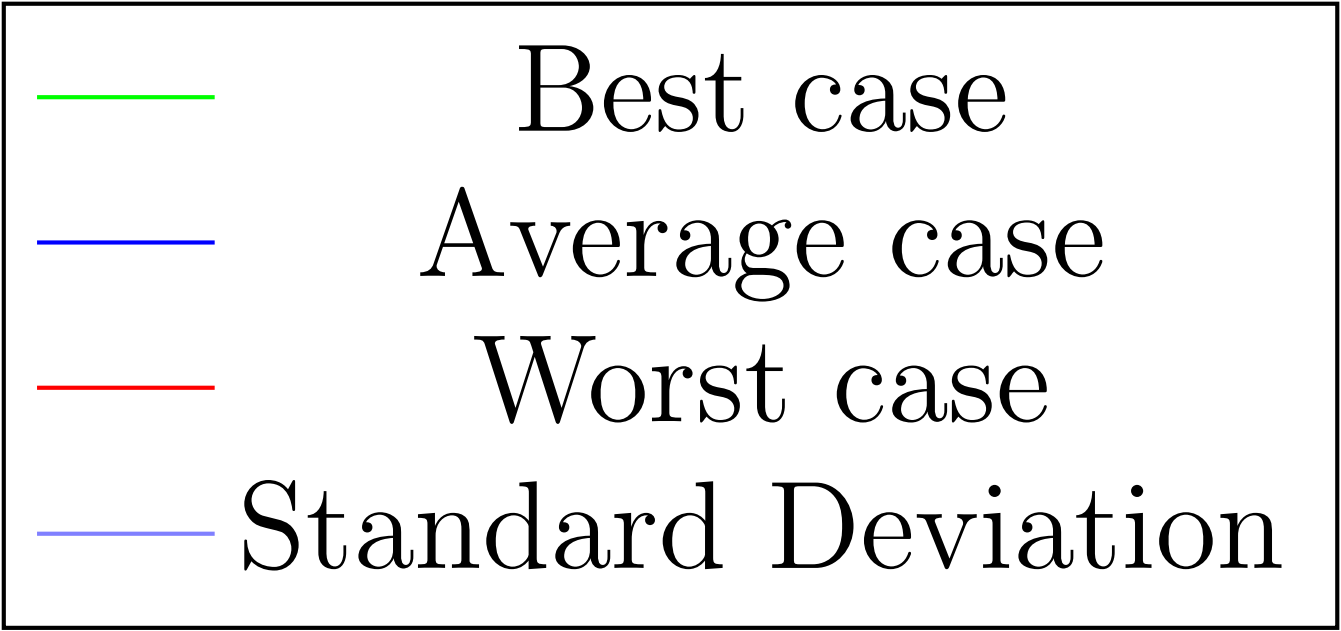
\includegraphics[scale=0.1]{chapters/res/generated_graph_legend.png}};
\end{tikzpicture}

\begin{figure}[H]
\vspace*{-1cm}
	\makebox[\linewidth][c]{%
	\begin{subfigure}[b]{0.7\textwidth}
		\centering
		\resizebox{0.9\linewidth}{!}{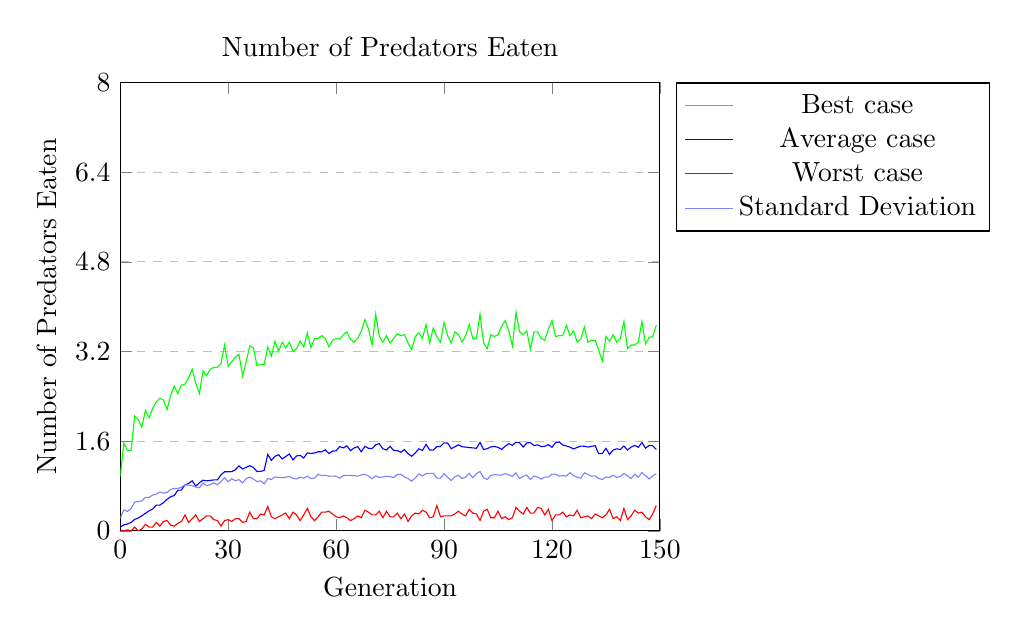
\begin{tikzpicture}
\begin{axis}[
	title={Number of Predators Eaten},
	xlabel={Generation},
	ylabel={Number of Predators Eaten},
	xmin=0, xmax=150,
	ymin=0, ymax=8,
	xtick={0.0,30.0,60.0,90.0,120.0,150.0},
	ytick={0.0,1.6,3.2,4.800000000000001,6.4,8.0},
	legend pos=outer north east,
	ymajorgrids=true,
	grid style=dashed,
]

\addplot[
	color=green,
	]
	coordinates {
	(0,0.9666666666666666)(1,1.5666666666666669)(2,1.4333333333333331)(3,1.4333333333333333)(4,2.05)(5,1.9833333333333336)(6,1.8500000000000003)(7,2.15)(8,2.016666666666667)(9,2.1833333333333336)(10,2.2999999999999994)(11,2.3666666666666676)(12,2.3333333333333335)(13,2.166666666666667)(14,2.416666666666667)(15,2.583333333333333)(16,2.4499999999999997)(17,2.6)(18,2.616666666666667)(19,2.7333333333333334)(20,2.8833333333333333)(21,2.6333333333333333)(22,2.4500000000000006)(23,2.85)(24,2.766666666666666)(25,2.8833333333333333)(26,2.916666666666667)(27,2.9166666666666665)(28,2.9833333333333325)(29,3.3166666666666664)(30,2.9333333333333327)(31,3.0166666666666666)(32,3.0999999999999996)(33,3.1499999999999995)(34,2.766666666666667)(35,3.0166666666666666)(36,3.3000000000000007)(37,3.2666666666666666)(38,2.9499999999999997)(39,2.966666666666667)(40,2.9666666666666663)(41,3.2833333333333328)(42,3.1166666666666667)(43,3.383333333333333)(44,3.2)(45,3.3666666666666663)(46,3.2666666666666666)(47,3.3666666666666667)(48,3.1999999999999997)(49,3.2499999999999996)(50,3.383333333333333)(51,3.2833333333333337)(52,3.533333333333333)(53,3.266666666666667)(54,3.433333333333333)(55,3.433333333333334)(56,3.483333333333333)(57,3.433333333333333)(58,3.283333333333333)(59,3.399999999999999)(60,3.4333333333333327)(61,3.4166666666666665)(62,3.5)(63,3.5500000000000003)(64,3.416666666666667)(65,3.366666666666667)(66,3.4333333333333336)(67,3.5666666666666664)(68,3.7666666666666666)(69,3.5999999999999996)(70,3.316666666666667)(71,3.8666666666666667)(72,3.466666666666666)(73,3.366666666666667)(74,3.4833333333333334)(75,3.349999999999999)(76,3.4333333333333345)(77,3.5166666666666657)(78,3.483333333333333)(79,3.5)(80,3.3500000000000005)(81,3.233333333333333)(82,3.466666666666667)(83,3.533333333333333)(84,3.4333333333333327)(85,3.6833333333333336)(86,3.3500000000000005)(87,3.6166666666666667)(88,3.4666666666666663)(89,3.3666666666666667)(90,3.716666666666667)(91,3.4833333333333334)(92,3.349999999999999)(93,3.549999999999999)(94,3.5)(95,3.366666666666667)(96,3.4833333333333325)(97,3.683333333333333)(98,3.4333333333333336)(99,3.4333333333333336)(100,3.8666666666666676)(101,3.3499999999999996)(102,3.2499999999999996)(103,3.5)(104,3.466666666666666)(105,3.4999999999999996)(106,3.650000000000001)(107,3.7499999999999996)(108,3.5666666666666664)(109,3.3)(110,3.9)(111,3.55)(112,3.5)(113,3.566666666666666)(114,3.2333333333333334)(115,3.55)(116,3.55)(117,3.433333333333333)(118,3.3999999999999995)(119,3.5999999999999996)(120,3.7499999999999996)(121,3.466666666666667)(122,3.483333333333333)(123,3.483333333333333)(124,3.6666666666666665)(125,3.4833333333333325)(126,3.5666666666666664)(127,3.3666666666666663)(128,3.416666666666667)(129,3.6333333333333333)(130,3.3666666666666663)(131,3.399999999999999)(132,3.3999999999999995)(133,3.216666666666667)(134,3.033333333333333)(135,3.4666666666666663)(136,3.383333333333333)(137,3.499999999999999)(138,3.3666666666666667)(139,3.433333333333334)(140,3.7333333333333334)(141,3.2500000000000004)(142,3.3166666666666664)(143,3.3166666666666673)(144,3.366666666666666)(145,3.733333333333333)(146,3.333333333333333)(147,3.45)(148,3.466666666666666)(149,3.6666666666666665)
	};
	\addlegendentry{Best case}
\addplot[
	color=blue,
	]
	coordinates {
	(0,0.06597222222222222)(1,0.10555555555555557)(2,0.12222222222222222)(3,0.14930555555555552)(4,0.2041666666666667)(5,0.2277777777777778)(6,0.2694444444444445)(7,0.31180555555555556)(8,0.35625)(9,0.38819444444444445)(10,0.4583333333333333)(11,0.4590277777777777)(12,0.5020833333333333)(13,0.5625000000000001)(14,0.6083333333333333)(15,0.6298611111111111)(16,0.7243055555555556)(17,0.7270833333333333)(18,0.8208333333333333)(19,0.8458333333333333)(20,0.8916666666666668)(21,0.7972222222222223)(22,0.8576388888888888)(23,0.9027777777777778)(24,0.8909722222222223)(25,0.8993055555555554)(26,0.9083333333333332)(27,0.9083333333333333)(28,1.0)(29,1.0534722222222221)(30,1.0541666666666667)(31,1.0555555555555556)(32,1.0909722222222222)(33,1.158333333333333)(34,1.1020833333333333)(35,1.1333333333333335)(36,1.1618055555555558)(37,1.1319444444444442)(38,1.0583333333333333)(39,1.0611111111111111)(40,1.0777777777777777)(41,1.363888888888889)(42,1.25625)(43,1.3291666666666664)(44,1.3590277777777777)(45,1.2826388888888889)(46,1.3256944444444447)(47,1.371527777777778)(48,1.2652777777777775)(49,1.3354166666666665)(50,1.3472222222222225)(51,1.298611111111111)(52,1.3902777777777777)(53,1.379861111111111)(54,1.3888888888888888)(55,1.4104166666666669)(56,1.409722222222222)(57,1.4451388888888888)(58,1.3791666666666667)(59,1.423611111111111)(60,1.4263888888888887)(61,1.5020833333333334)(62,1.4791666666666663)(63,1.5166666666666668)(64,1.430555555555556)(65,1.4777777777777776)(66,1.5020833333333334)(67,1.4111111111111114)(68,1.507638888888889)(69,1.472916666666667)(70,1.4666666666666668)(71,1.535416666666667)(72,1.5548611111111108)(73,1.4638888888888888)(74,1.4409722222222219)(75,1.5083333333333335)(76,1.4333333333333331)(77,1.4312499999999997)(78,1.402083333333333)(79,1.4500000000000002)(80,1.3763888888888889)(81,1.3305555555555555)(82,1.3888888888888884)(83,1.4631944444444447)(84,1.4340277777777777)(85,1.5416666666666665)(86,1.4437499999999999)(87,1.4388888888888893)(88,1.5013888888888887)(89,1.5048611111111112)(90,1.570138888888889)(91,1.5659722222222225)(92,1.4645833333333331)(93,1.4999999999999996)(94,1.5340277777777784)(95,1.5006944444444446)(96,1.49375)(97,1.4854166666666668)(98,1.479861111111111)(99,1.4729166666666667)(100,1.5777777777777777)(101,1.4493055555555556)(102,1.465972222222222)(103,1.498611111111111)(104,1.5055555555555555)(105,1.4888888888888892)(106,1.4541666666666668)(107,1.5090277777777776)(108,1.5555555555555558)(109,1.5243055555555558)(110,1.5798611111111107)(111,1.5715277777777774)(112,1.4958333333333333)(113,1.5701388888888888)(114,1.5743055555555556)(115,1.520833333333333)(116,1.5340277777777778)(117,1.503472222222222)(118,1.5083333333333333)(119,1.5381944444444444)(120,1.4902777777777776)(121,1.571527777777778)(122,1.5847222222222221)(123,1.5319444444444448)(124,1.5145833333333332)(125,1.4930555555555558)(126,1.4618055555555554)(127,1.4868055555555553)(128,1.5118055555555556)(129,1.5090277777777779)(130,1.4951388888888888)(131,1.5069444444444442)(132,1.5194444444444446)(133,1.3756944444444443)(134,1.3798611111111112)(135,1.4722222222222219)(136,1.3625)(137,1.4430555555555553)(138,1.4631944444444447)(139,1.4499999999999997)(140,1.5124999999999997)(141,1.4416666666666667)(142,1.4937500000000001)(143,1.5243055555555558)(144,1.4902777777777778)(145,1.5749999999999997)(146,1.4749999999999999)(147,1.522916666666667)(148,1.5180555555555555)(149,1.450694444444444)
	};
	\addlegendentry{Average case}
\addplot[
	color=red,
	]
	coordinates {
	(0,0.0)(1,0.0)(2,0.016666666666666666)(3,0.0)(4,0.06666666666666667)(5,0.0)(6,0.03333333333333333)(7,0.11666666666666667)(8,0.06666666666666667)(9,0.06666666666666667)(10,0.15)(11,0.08333333333333333)(12,0.16666666666666666)(13,0.18333333333333332)(14,0.1)(15,0.08333333333333333)(16,0.13333333333333333)(17,0.16666666666666666)(18,0.2833333333333333)(19,0.15)(20,0.21666666666666665)(21,0.2833333333333333)(22,0.16666666666666666)(23,0.21666666666666665)(24,0.26666666666666666)(25,0.26666666666666666)(26,0.19999999999999998)(27,0.18333333333333332)(28,0.08333333333333334)(29,0.18333333333333332)(30,0.19999999999999998)(31,0.16666666666666666)(32,0.21666666666666665)(33,0.21666666666666665)(34,0.15)(35,0.16666666666666666)(36,0.3333333333333333)(37,0.21666666666666665)(38,0.21666666666666665)(39,0.3)(40,0.2833333333333333)(41,0.4333333333333333)(42,0.24999999999999997)(43,0.21666666666666665)(44,0.24999999999999997)(45,0.2833333333333333)(46,0.31666666666666665)(47,0.21666666666666665)(48,0.3333333333333333)(49,0.2833333333333333)(50,0.18333333333333332)(51,0.2833333333333333)(52,0.39999999999999997)(53,0.24999999999999997)(54,0.18333333333333332)(55,0.24999999999999997)(56,0.3333333333333333)(57,0.3333333333333333)(58,0.35)(59,0.3)(60,0.24999999999999997)(61,0.2333333333333333)(62,0.26666666666666666)(63,0.2333333333333333)(64,0.18333333333333332)(65,0.21666666666666665)(66,0.26666666666666666)(67,0.2333333333333333)(68,0.36666666666666664)(69,0.3333333333333333)(70,0.2833333333333333)(71,0.2833333333333333)(72,0.35)(73,0.2333333333333333)(74,0.35)(75,0.24999999999999997)(76,0.24999999999999997)(77,0.31666666666666665)(78,0.21666666666666665)(79,0.3)(80,0.16666666666666666)(81,0.26666666666666666)(82,0.31666666666666665)(83,0.3)(84,0.36666666666666664)(85,0.3333333333333333)(86,0.2333333333333333)(87,0.24999999999999997)(88,0.44999999999999996)(89,0.24999999999999997)(90,0.26666666666666666)(91,0.26666666666666666)(92,0.26666666666666666)(93,0.3)(94,0.35)(95,0.3)(96,0.26666666666666666)(97,0.3833333333333333)(98,0.31666666666666665)(99,0.3)(100,0.18333333333333332)(101,0.35)(102,0.3833333333333333)(103,0.2333333333333333)(104,0.2333333333333333)(105,0.35)(106,0.21666666666666665)(107,0.24999999999999997)(108,0.19999999999999998)(109,0.2333333333333333)(110,0.41666666666666663)(111,0.35)(112,0.3)(113,0.41666666666666663)(114,0.31666666666666665)(115,0.31666666666666665)(116,0.41666666666666663)(117,0.39999999999999997)(118,0.2833333333333333)(119,0.3833333333333333)(120,0.18333333333333332)(121,0.2833333333333333)(122,0.2833333333333333)(123,0.3333333333333333)(124,0.24999999999999997)(125,0.2833333333333333)(126,0.26666666666666666)(127,0.36666666666666664)(128,0.2333333333333333)(129,0.24999999999999997)(130,0.26666666666666666)(131,0.21666666666666665)(132,0.3)(133,0.26666666666666666)(134,0.2333333333333333)(135,0.2833333333333333)(136,0.3833333333333333)(137,0.21666666666666665)(138,0.24999999999999997)(139,0.18333333333333332)(140,0.39999999999999997)(141,0.19999999999999998)(142,0.26666666666666666)(143,0.36666666666666664)(144,0.31666666666666665)(145,0.3333333333333333)(146,0.24999999999999997)(147,0.19999999999999998)(148,0.3)(149,0.44999999999999996)
	};
	\addlegendentry{Worst case}
\addplot[
	color=blue!50,
	]
	coordinates {
	(0,0.22810186512317995)(1,0.3718097332768811)(2,0.345647402635599)(3,0.39699357623545967)(4,0.5138792555180911)(5,0.5206370865039666)(6,0.5354322880656994)(7,0.5959918288673569)(8,0.5957464980983094)(9,0.6381545461207714)(10,0.6544157192161484)(11,0.6927992034441525)(12,0.6722084507491709)(13,0.6843365883572965)(14,0.7384416963839964)(15,0.7553805146012672)(16,0.7567879875086504)(17,0.7761000580438222)(18,0.8239608598665922)(19,0.8141765811345567)(20,0.8059054603391009)(21,0.7827695395066535)(22,0.7685798512811592)(23,0.8545075912627764)(24,0.8066600194512461)(25,0.8213047161793012)(26,0.8566928186325042)(27,0.8219235106348346)(28,0.8818150722779325)(29,0.9483172788083861)(30,0.8759037593822429)(31,0.928085110238431)(32,0.8933512538685642)(33,0.9145676016751958)(34,0.8540885600591401)(35,0.9361875717102862)(36,0.9532635109306814)(37,0.9248288480881136)(38,0.8780358726506764)(39,0.8920947846161121)(40,0.8389079397070467)(41,0.9310517560644359)(42,0.9169672329669347)(43,0.9626393230017223)(44,0.953305984898185)(45,0.9475155563329191)(46,0.9563120633890103)(47,0.9690109120939004)(48,0.9370607511828415)(49,0.9251085904346795)(50,0.9593348140607003)(51,0.9388820833026523)(52,0.9772060224313383)(53,0.9327708529184457)(54,0.9412102328931546)(55,1.0077411580389004)(56,0.9852037990060252)(57,0.9911527973635053)(58,0.9739897240274592)(59,0.9762958851755198)(60,0.9728815797212503)(61,0.9397801191846543)(62,0.9860176940119886)(63,0.9887585575026453)(64,0.9878949236675736)(65,0.9857002506497867)(66,0.9742204622105117)(67,0.997738909615304)(68,1.0070425414875266)(69,0.977663045346536)(70,0.928886568602237)(71,0.9791505985330582)(72,0.9545986319347426)(73,0.9616850879978396)(74,0.9732365499001447)(75,0.9646654709337494)(76,0.9508629094932712)(77,1.0025603129489447)(78,1.0095566600655457)(79,0.9595891281644218)(80,0.9337702023850106)(81,0.8861973519209494)(82,0.9433294526574671)(83,1.0152919365875552)(84,0.9787093157423733)(85,1.0222555976967989)(86,1.0247018937565666)(87,1.0262721417066973)(88,0.9412691816448212)(89,0.9407486267702396)(90,1.0194751751230433)(91,0.955970674775724)(92,0.8982605274530155)(93,0.9641212560889841)(94,0.9929408862575011)(95,0.9337221659166333)(96,0.9572120942865925)(97,1.0259309967342551)(98,0.9501115634388491)(99,1.019286121940842)(100,1.0586653743886223)(101,0.944150328954389)(102,0.9165038721252468)(103,0.9882369427730343)(104,1.0024095780547078)(105,0.997845039428861)(106,0.9929675230837386)(107,1.0209746253543222)(108,0.9964515312484529)(109,0.9732781796446134)(110,1.0326336414888901)(111,0.9319156849314015)(112,0.9716152138162422)(113,0.9957941705810749)(114,0.9173588293084006)(115,0.9782184152846188)(116,0.9597984307842808)(117,0.9224617398001695)(118,0.9582514881452882)(119,0.958707393381238)(120,1.0129407727703712)(121,1.009816594443192)(122,0.9762712582599299)(123,0.9847047252553303)(124,0.977086094849565)(125,1.0368969148123457)(126,0.9844155409431966)(127,0.9564477843400175)(128,0.9369375197935595)(129,1.0356988710778785)(130,1.006687832266945)(131,0.9736212916755186)(132,0.9818050306273509)(133,0.9314510779420476)(134,0.9174090582062905)(135,0.9607146057643011)(136,0.9477226927053267)(137,0.9946920048277378)(138,0.9529447551456616)(139,0.9707813834396313)(140,1.021358396528527)(141,0.9813965194540895)(142,0.9343798771309901)(143,1.009943885726864)(144,0.9544205477403176)(145,1.042712213375269)(146,0.9850693099959399)(147,0.9250773473950887)(148,0.981919924129806)(149,1.0147175457773097)
	};
	\addlegendentry{Standard Deviation}
\end{axis}
\end{tikzpicture}
}
		\caption{Some sample caption}
	\end{subfigure}%
	\begin{subfigure}[b]{0.7\textwidth}	
		\centering
		\resizebox{0.9\linewidth}{!}{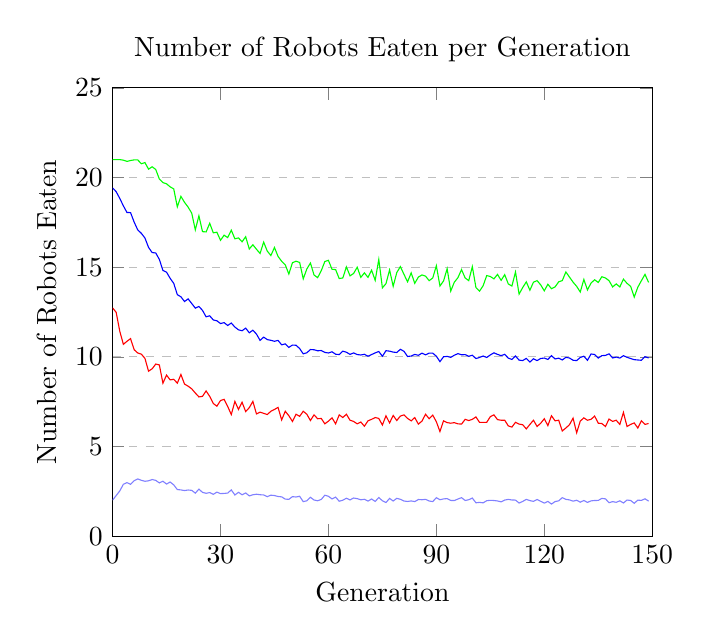
\begin{tikzpicture}
\begin{axis}[
	title={Number of Robots Eaten per Generation},
	xlabel={Generation},
	ylabel={Number of Robots Eaten},
	xmin=0, xmax=150,
	ymin=0, ymax=25,
	xtick={0.0,30.0,60.0,90.0,120.0,150.0},
	ytick={0.0,5.0,10.0,15.0,20.0,25.0},
	ymajorgrids=true,
	grid style=dashed,
]

\addplot[
	color=green,
	]
	coordinates {
	(0,21.000000000000007)(1,21.000000000000007)(2,21.000000000000007)(3,20.966666666666672)(4,20.900000000000006)(5,20.950000000000006)(6,20.98333333333334)(7,20.98333333333334)(8,20.766666666666673)(9,20.83333333333334)(10,20.466666666666672)(11,20.600000000000005)(12,20.450000000000003)(13,19.91666666666667)(14,19.716666666666672)(15,19.650000000000006)(16,19.483333333333338)(17,19.366666666666667)(18,18.366666666666667)(19,18.950000000000003)(20,18.61666666666667)(21,18.349999999999998)(22,18.016666666666666)(23,17.083333333333332)(24,17.866666666666664)(25,16.983333333333327)(26,16.96666666666667)(27,17.45)(28,16.916666666666664)(29,16.95)(30,16.5)(31,16.78333333333333)(32,16.649999999999995)(33,17.066666666666666)(34,16.583333333333332)(35,16.633333333333336)(36,16.416666666666664)(37,16.7)(38,16.016666666666666)(39,16.25)(40,16.0)(41,15.766666666666664)(42,16.4)(43,15.899999999999997)(44,15.649999999999999)(45,16.1)(46,15.600000000000001)(47,15.333333333333332)(48,15.133333333333335)(49,14.616666666666664)(50,15.25)(51,15.333333333333334)(52,15.266666666666666)(53,14.349999999999998)(54,14.900000000000002)(55,15.233333333333333)(56,14.566666666666665)(57,14.416666666666668)(58,14.8)(59,15.316666666666668)(60,15.383333333333331)(61,14.883333333333333)(62,14.866666666666665)(63,14.366666666666667)(64,14.399999999999999)(65,15.016666666666664)(66,14.516666666666667)(67,14.649999999999997)(68,14.999999999999998)(69,14.433333333333334)(70,14.683333333333332)(71,14.433333333333332)(72,14.833333333333332)(73,14.266666666666667)(74,15.433333333333332)(75,13.850000000000001)(76,14.083333333333332)(77,14.849999999999998)(78,13.933333333333334)(79,14.699999999999998)(80,15.033333333333333)(81,14.600000000000001)(82,14.183333333333334)(83,14.683333333333334)(84,14.100000000000001)(85,14.450000000000001)(86,14.566666666666663)(87,14.5)(88,14.250000000000002)(89,14.4)(90,15.083333333333334)(91,13.950000000000001)(92,14.233333333333333)(93,14.916666666666664)(94,13.666666666666671)(95,14.166666666666663)(96,14.416666666666668)(97,14.866666666666665)(98,14.4)(99,14.25)(100,15.033333333333333)(101,13.866666666666664)(102,13.66666666666667)(103,13.966666666666665)(104,14.533333333333333)(105,14.483333333333334)(106,14.350000000000001)(107,14.600000000000001)(108,14.26666666666667)(109,14.583333333333332)(110,14.066666666666666)(111,13.95)(112,14.733333333333334)(113,13.499999999999998)(114,13.866666666666665)(115,14.183333333333334)(116,13.716666666666669)(117,14.166666666666666)(118,14.249999999999998)(119,14.016666666666667)(120,13.683333333333332)(121,14.05)(122,13.8)(123,13.899999999999999)(124,14.183333333333334)(125,14.25)(126,14.733333333333336)(127,14.450000000000003)(128,14.166666666666664)(129,13.933333333333332)(130,13.616666666666665)(131,14.316666666666666)(132,13.733333333333333)(133,14.116666666666665)(134,14.299999999999999)(135,14.15)(136,14.46666666666667)(137,14.400000000000004)(138,14.250000000000002)(139,13.9)(140,14.066666666666668)(141,13.899999999999999)(142,14.333333333333332)(143,14.100000000000001)(144,13.933333333333334)(145,13.333333333333336)(146,13.883333333333333)(147,14.249999999999998)(148,14.6)(149,14.150000000000002)
	};
\addplot[
	color=blue,
	]
	coordinates {
	(0,19.422916666666666)(1,19.211111111111116)(2,18.837500000000002)(3,18.42291666666667)(4,18.050694444444446)(5,18.045833333333338)(6,17.51319444444444)(7,17.07986111111111)(8,16.889583333333338)(9,16.62708333333333)(10,16.105555555555554)(11,15.81736111111111)(12,15.792361111111113)(13,15.43611111111111)(14,14.817361111111111)(15,14.725000000000001)(16,14.38055555555556)(17,14.099999999999998)(18,13.46875)(19,13.349305555555556)(20,13.087500000000004)(21,13.231944444444446)(22,12.977083333333335)(23,12.718055555555559)(24,12.81111111111111)(25,12.592361111111112)(26,12.23263888888889)(27,12.290972222222223)(28,12.05833333333333)(29,12.011805555555558)(30,11.858333333333336)(31,11.909027777777778)(32,11.749999999999998)(33,11.886805555555554)(34,11.661805555555556)(35,11.508333333333335)(36,11.455555555555554)(37,11.602777777777776)(38,11.34375)(39,11.48611111111111)(40,11.271527777777775)(41,10.918750000000003)(42,11.100694444444445)(43,10.963194444444445)(44,10.922916666666667)(45,10.869444444444445)(46,10.91875)(47,10.670138888888888)(48,10.726388888888886)(49,10.528472222222222)(50,10.658333333333333)(51,10.64722222222222)(52,10.465277777777779)(53,10.16875)(54,10.22847222222222)(55,10.408333333333335)(56,10.397222222222222)(57,10.338888888888892)(58,10.354861111111111)(59,10.249305555555555)(60,10.216666666666667)(61,10.283333333333335)(62,10.147222222222222)(63,10.128472222222221)(64,10.318055555555555)(65,10.257638888888888)(66,10.13888888888889)(67,10.220833333333333)(68,10.129166666666666)(69,10.104166666666668)(70,10.143749999999999)(71,10.035416666666668)(72,10.130555555555556)(73,10.220833333333335)(74,10.299999999999997)(75,10.034027777777778)(76,10.343055555555555)(77,10.319444444444445)(78,10.264583333333333)(79,10.244444444444445)(80,10.420833333333334)(81,10.310416666666669)(82,10.022222222222222)(83,10.045138888888888)(84,10.136805555555556)(85,10.086111111111112)(86,10.20625)(87,10.113194444444446)(88,10.20833333333333)(89,10.206249999999999)(90,10.037499999999998)(91,9.734027777777778)(92,10.005555555555555)(93,10.027083333333334)(94,9.971527777777778)(95,10.093055555555557)(96,10.180555555555557)(97,10.113194444444444)(98,10.127083333333335)(99,10.033333333333333)(100,10.090972222222218)(101,9.904166666666667)(102,9.968055555555555)(103,10.047222222222224)(104,9.965972222222224)(105,10.107638888888888)(106,10.22638888888889)(107,10.137499999999998)(108,10.068750000000001)(109,10.140972222222224)(110,9.929861111111112)(111,9.855555555555556)(112,10.04722222222222)(113,9.81736111111111)(114,9.792361111111111)(115,9.915277777777778)(116,9.709722222222222)(117,9.894444444444444)(118,9.792361111111113)(119,9.910416666666665)(120,9.934027777777777)(121,9.856250000000001)(122,10.068055555555555)(123,9.882638888888888)(124,9.929166666666667)(125,9.827083333333333)(126,9.973611111111111)(127,9.936805555555557)(128,9.811111111111112)(129,9.793055555555554)(130,9.96597222222222)(131,10.036805555555555)(132,9.808333333333334)(133,10.162499999999998)(134,10.129861111111111)(135,9.933333333333332)(136,10.06875)(137,10.080555555555556)(138,10.16875)(139,9.939583333333333)(140,9.9875)(141,9.933333333333334)(142,10.068055555555555)(143,9.975000000000001)(144,9.90763888888889)(145,9.84375)(146,9.825694444444446)(147,9.810416666666669)(148,10.009722222222223)(149,9.938888888888888)
	};
\addplot[
	color=red,
	]
	coordinates {
	(0,12.733333333333336)(1,12.483333333333334)(2,11.433333333333334)(3,10.700000000000001)(4,10.866666666666667)(5,11.016666666666667)(6,10.400000000000002)(7,10.216666666666667)(8,10.149999999999999)(9,9.916666666666664)(10,9.200000000000003)(11,9.333333333333336)(12,9.600000000000001)(13,9.55)(14,8.533333333333335)(15,8.983333333333334)(16,8.716666666666667)(17,8.75)(18,8.533333333333333)(19,9.016666666666667)(20,8.483333333333333)(21,8.366666666666667)(22,8.216666666666667)(23,7.9833333333333325)(24,7.7666666666666675)(25,7.799999999999998)(26,8.1)(27,7.799999999999999)(28,7.399999999999998)(29,7.25)(30,7.566666666666668)(31,7.633333333333333)(32,7.233333333333333)(33,6.783333333333332)(34,7.516666666666668)(35,7.0666666666666655)(36,7.466666666666668)(37,6.949999999999999)(38,7.166666666666666)(39,7.516666666666667)(40,6.8166666666666655)(41,6.916666666666665)(42,6.8500000000000005)(43,6.783333333333335)(44,6.966666666666666)(45,7.066666666666667)(46,7.183333333333334)(47,6.483333333333332)(48,6.966666666666666)(49,6.716666666666666)(50,6.4)(51,6.8)(52,6.683333333333334)(53,6.966666666666666)(54,6.800000000000001)(55,6.4499999999999975)(56,6.766666666666666)(57,6.55)(58,6.566666666666666)(59,6.266666666666666)(60,6.416666666666666)(61,6.6)(62,6.266666666666666)(63,6.766666666666667)(64,6.616666666666666)(65,6.8)(66,6.466666666666666)(67,6.4)(68,6.266666666666666)(69,6.366666666666667)(70,6.133333333333335)(71,6.433333333333333)(72,6.5166666666666675)(73,6.616666666666666)(74,6.5666666666666655)(75,6.199999999999999)(76,6.716666666666669)(77,6.316666666666666)(78,6.7333333333333325)(79,6.449999999999998)(80,6.7)(81,6.766666666666667)(82,6.566666666666666)(83,6.433333333333334)(84,6.616666666666667)(85,6.250000000000001)(86,6.416666666666666)(87,6.8)(88,6.549999999999999)(89,6.749999999999998)(90,6.383333333333335)(91,5.833333333333333)(92,6.433333333333334)(93,6.333333333333332)(94,6.3)(95,6.333333333333333)(96,6.266666666666666)(97,6.249999999999999)(98,6.516666666666666)(99,6.449999999999999)(100,6.516666666666667)(101,6.6499999999999995)(102,6.3500000000000005)(103,6.35)(104,6.349999999999999)(105,6.666666666666666)(106,6.766666666666667)(107,6.499999999999999)(108,6.466666666666667)(109,6.466666666666666)(110,6.149999999999999)(111,6.083333333333334)(112,6.35)(113,6.250000000000001)(114,6.216666666666668)(115,5.983333333333333)(116,6.2333333333333325)(117,6.466666666666667)(118,6.116666666666668)(119,6.300000000000001)(120,6.55)(121,6.166666666666668)(122,6.716666666666665)(123,6.433333333333333)(124,6.466666666666667)(125,5.866666666666667)(126,6.033333333333333)(127,6.216666666666667)(128,6.583333333333333)(129,5.766666666666666)(130,6.416666666666666)(131,6.6)(132,6.466666666666666)(133,6.516666666666666)(134,6.699999999999999)(135,6.3)(136,6.283333333333334)(137,6.116666666666666)(138,6.533333333333332)(139,6.3999999999999995)(140,6.466666666666665)(141,6.233333333333333)(142,6.8999999999999995)(143,6.116666666666665)(144,6.2333333333333325)(145,6.316666666666666)(146,6.033333333333333)(147,6.433333333333334)(148,6.2333333333333325)(149,6.283333333333334)
	};
\addplot[
	color=blue!50,
	]
	coordinates {
	(0,2.0113996005838635)(1,2.2655504562278455)(2,2.523428127338372)(3,2.893897423121901)(4,2.9871822928142326)(5,2.8918968080680627)(6,3.096152416787628)(7,3.1947663840800775)(8,3.116582184803458)(9,3.0625628948276606)(10,3.088398573928132)(11,3.1601776571620803)(12,3.11341262394878)(13,2.971398344151116)(14,3.06614123565838)(15,2.9060661139400845)(16,3.021158320712189)(17,2.861439826087297)(18,2.6003656040557708)(19,2.5806621327374137)(20,2.5448185766978018)(21,2.574726725943908)(22,2.5578593675944723)(23,2.40115494497435)(24,2.6247028738208273)(25,2.443123536140499)(26,2.3929554749092263)(27,2.431079502448026)(28,2.3358855371024196)(29,2.455976942365564)(30,2.375087540335267)(31,2.384771373914672)(32,2.404685694641398)(33,2.5816980161392284)(34,2.297047689823935)(35,2.4485912083596513)(36,2.3098481664582846)(37,2.41149041509496)(38,2.2471607125399964)(39,2.308838414195794)(40,2.341908447385709)(41,2.312535325828631)(42,2.298721389611761)(43,2.205061751636127)(44,2.2875895143938827)(45,2.266955033185302)(46,2.2139667780639236)(47,2.1935510635671744)(48,2.0687648634365234)(49,2.0545686330476727)(50,2.2055585186985605)(51,2.1850688892750294)(52,2.2269862286438173)(53,1.9264278418564131)(54,1.9738967352367478)(55,2.1690059870394753)(56,2.0173523025563607)(57,1.9767057087670006)(58,2.049017498246475)(59,2.285754671814331)(60,2.225965931591818)(61,2.0781486159288383)(62,2.178753197459309)(63,1.9483248658673213)(64,2.0077682344840406)(65,2.116536805925538)(66,2.0241064392397696)(67,2.128581489300377)(68,2.0936853665373265)(69,2.028433424718565)(70,2.056973610743671)(71,1.9568840865375499)(72,2.0762553542894326)(73,1.9379167376002602)(74,2.156396583454864)(75,1.974947342812672)(76,1.8791106317170232)(77,2.107867209533473)(78,1.9627413337381523)(79,2.1117674474423227)(80,2.0573151374234526)(81,1.962497890883103)(82,1.9370373765350182)(83,1.9651318768331705)(84,1.9309095516477237)(85,2.0455965865726524)(86,2.0335901945053156)(87,2.0553178281795685)(88,1.9630050391005152)(89,1.929738818337511)(90,2.1475524139172415)(91,2.032266524353691)(92,2.079539681480517)(93,2.096309181288721)(94,1.994101735474168)(95,1.9885174942042725)(96,2.072921590049966)(97,2.1491137043758153)(98,1.991836421647755)(99,2.0327704181702075)(100,2.127009120922501)(101,1.8627280658001233)(102,1.8843106883309968)(103,1.8600047687719843)(104,1.9781530489036958)(105,2.0004393939225618)(106,1.9905902184375726)(107,1.9650315763564947)(108,1.9162297980300185)(109,2.01450144528217)(110,2.0536696301117803)(111,2.018536108751344)(112,2.0141474454495207)(113,1.8483255759174422)(114,1.9378582863595812)(115,2.05349579201371)(116,1.9845712197978036)(117,1.9407422354604016)(118,2.048149155491315)(119,1.943493054279464)(120,1.845400689140209)(121,1.939649979266822)(122,1.7928649191375787)(123,1.929929208687165)(124,1.9714707615015763)(125,2.148818763612173)(126,2.054244734087596)(127,2.0251514333575074)(128,1.9530007698209328)(129,2.0028252223945135)(130,1.8980163699486958)(131,1.9903199966926706)(132,1.8843253066567944)(133,1.969885674032518)(134,1.991229157137803)(135,1.9944395098710415)(136,2.1089209643957108)(137,2.0818808510389504)(138,1.868140827387872)(139,1.9269487312153624)(140,1.888974106705156)(141,1.9719484911636793)(142,1.850660754242215)(143,2.0158816949093867)(144,1.9931779658014623)(145,1.8352893878127157)(146,2.009082649009219)(147,1.996841607573629)(148,2.085186695851752)(149,1.956308451005405)
	};
\end{axis}
\end{tikzpicture}
}
		\caption{Some sample caption}
	\end{subfigure}%
}
\\
\\
\\
	\makebox[\linewidth][c]{%
	\begin{subfigure}[b]{0.7\textwidth}
		\centering
		\resizebox{0.9\linewidth}{!}{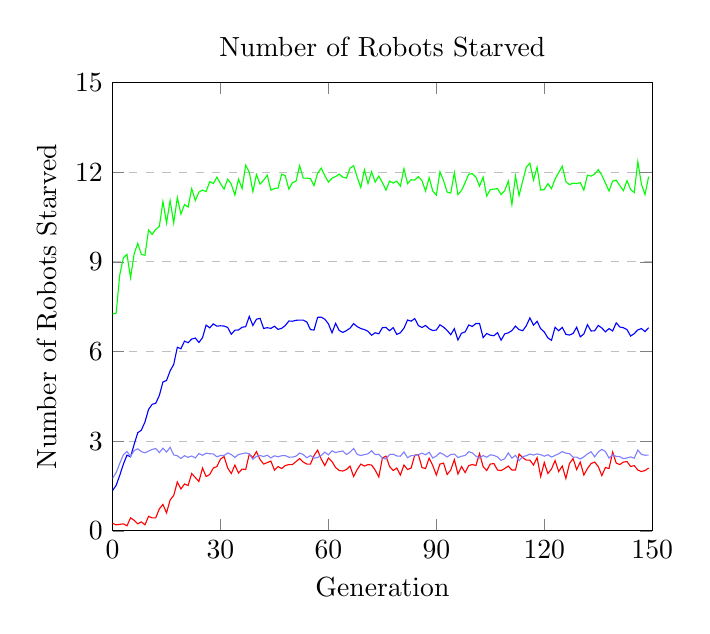
\begin{tikzpicture}
\begin{axis}[
	title={Number of Robots Starved},
	xlabel={Generation},
	ylabel={Number of Robots Starved},
	xmin=0, xmax=150,
	ymin=0, ymax=15,
	xtick={0.0,30.0,60.0,90.0,120.0,150.0},
	ytick={0.0,3.0,6.0,9.0,12.0,15.0},
	ymajorgrids=true,
	grid style=dashed,
]

\addplot[
	color=green,
	]
	coordinates {
	(0,7.250000000000002)(1,7.283333333333334)(2,8.566666666666668)(3,9.133333333333331)(4,9.25)(5,8.466666666666667)(6,9.266666666666667)(7,9.616666666666665)(8,9.25)(9,9.216666666666665)(10,10.066666666666666)(11,9.916666666666668)(12,10.083333333333332)(13,10.183333333333334)(14,11.01666666666667)(15,10.3)(16,11.050000000000002)(17,10.3)(18,11.15)(19,10.600000000000001)(20,10.916666666666666)(21,10.833333333333336)(22,11.450000000000003)(23,11.049999999999999)(24,11.333333333333332)(25,11.399999999999999)(26,11.349999999999998)(27,11.683333333333334)(28,11.616666666666667)(29,11.833333333333334)(30,11.616666666666669)(31,11.433333333333335)(32,11.766666666666666)(33,11.599999999999998)(34,11.233333333333334)(35,11.766666666666667)(36,11.450000000000001)(37,12.233333333333334)(38,12.000000000000002)(39,11.35)(40,11.916666666666664)(41,11.6)(42,11.73333333333333)(43,11.9)(44,11.399999999999997)(45,11.45)(46,11.466666666666669)(47,11.933333333333334)(48,11.883333333333333)(49,11.433333333333335)(50,11.649999999999999)(51,11.7)(52,12.216666666666667)(53,11.799999999999999)(54,11.800000000000004)(55,11.783333333333333)(56,11.55)(57,11.966666666666665)(58,12.133333333333335)(59,11.883333333333335)(60,11.666666666666668)(61,11.800000000000002)(62,11.849999999999998)(63,11.93333333333333)(64,11.833333333333332)(65,11.799999999999997)(66,12.133333333333335)(67,12.216666666666669)(68,11.833333333333334)(69,11.48333333333333)(70,12.083333333333332)(71,11.616666666666667)(72,12.016666666666666)(73,11.666666666666668)(74,11.866666666666667)(75,11.65)(76,11.399999999999999)(77,11.700000000000001)(78,11.633333333333335)(79,11.700000000000001)(80,11.533333333333335)(81,12.116666666666667)(82,11.616666666666667)(83,11.75)(84,11.733333333333333)(85,11.85)(86,11.716666666666669)(87,11.366666666666667)(88,11.816666666666666)(89,11.366666666666667)(90,11.233333333333333)(91,12.016666666666667)(92,11.716666666666667)(93,11.333333333333336)(94,11.299999999999999)(95,11.983333333333333)(96,11.249999999999998)(97,11.383333333333335)(98,11.650000000000002)(99,11.93333333333333)(100,11.950000000000001)(101,11.833333333333334)(102,11.533333333333331)(103,11.833333333333334)(104,11.200000000000001)(105,11.416666666666666)(106,11.43333333333333)(107,11.45)(108,11.25)(109,11.383333333333333)(110,11.699999999999998)(111,10.916666666666666)(112,11.866666666666667)(113,11.216666666666665)(114,11.700000000000001)(115,12.166666666666668)(116,12.3)(117,11.733333333333333)(118,12.166666666666666)(119,11.4)(120,11.416666666666668)(121,11.616666666666667)(122,11.45)(123,11.766666666666667)(124,11.983333333333333)(125,12.200000000000001)(126,11.683333333333334)(127,11.583333333333336)(128,11.633333333333335)(129,11.616666666666669)(130,11.650000000000002)(131,11.4)(132,11.900000000000002)(133,11.866666666666667)(134,11.933333333333334)(135,12.083333333333332)(136,11.9)(137,11.633333333333333)(138,11.366666666666667)(139,11.700000000000001)(140,11.733333333333333)(141,11.55)(142,11.383333333333333)(143,11.716666666666665)(144,11.416666666666666)(145,11.316666666666665)(146,12.349999999999998)(147,11.600000000000001)(148,11.25)(149,11.849999999999998)
	};
\addplot[
	color=blue,
	]
	coordinates {
	(0,1.3486111111111112)(1,1.5208333333333328)(2,1.8583333333333325)(3,2.2298611111111115)(4,2.5305555555555554)(5,2.4756944444444446)(6,2.890277777777778)(7,3.2819444444444446)(8,3.3680555555555562)(9,3.6381944444444447)(10,4.059722222222222)(11,4.232638888888889)(12,4.266666666666667)(13,4.527083333333333)(14,4.980555555555556)(15,5.029166666666667)(16,5.352083333333334)(17,5.567361111111111)(18,6.1409722222222225)(19,6.093055555555556)(20,6.345833333333333)(21,6.293750000000001)(22,6.415972222222222)(23,6.449305555555555)(24,6.302083333333333)(25,6.459027777777778)(26,6.88263888888889)(27,6.790972222222222)(28,6.922222222222224)(29,6.846527777777776)(30,6.860416666666667)(31,6.850694444444446)(32,6.804861111111113)(33,6.575694444444444)(34,6.711111111111111)(35,6.719444444444444)(36,6.811111111111112)(37,6.829861111111111)(38,7.172916666666666)(39,6.870833333333333)(40,7.0791666666666675)(41,7.1090277777777775)(42,6.770138888888889)(43,6.796527777777778)(44,6.772222222222222)(45,6.844444444444444)(46,6.736805555555556)(47,6.776388888888889)(48,6.865277777777778)(49,7.019444444444445)(50,7.0125)(51,7.043055555555554)(52,7.051388888888889)(53,7.050000000000001)(54,6.986805555555556)(55,6.731249999999999)(56,6.717361111111111)(57,7.143055555555554)(58,7.147916666666667)(59,7.0791666666666675)(60,6.924305555555556)(61,6.624999999999999)(62,6.9416666666666655)(63,6.702777777777779)(64,6.6402777777777775)(65,6.699305555555554)(66,6.779166666666668)(67,6.9312499999999995)(68,6.832638888888889)(69,6.767361111111111)(70,6.732638888888888)(71,6.675694444444443)(72,6.542361111111111)(73,6.62638888888889)(74,6.590972222222223)(75,6.795833333333333)(76,6.804166666666666)(77,6.69375)(78,6.797916666666666)(79,6.571527777777779)(80,6.626388888888888)(81,6.780555555555556)(82,7.054861111111112)(83,7.014583333333332)(84,7.10138888888889)(85,6.865972222222222)(86,6.802777777777777)(87,6.872222222222223)(88,6.759722222222222)(89,6.7020833333333325)(90,6.717361111111111)(91,6.892361111111111)(92,6.815277777777778)(93,6.703472222222223)(94,6.561111111111112)(95,6.761111111111112)(96,6.384027777777778)(97,6.612499999999999)(98,6.654166666666668)(99,6.886805555555556)(100,6.838194444444444)(101,6.936805555555557)(102,6.938194444444443)(103,6.463194444444444)(104,6.601388888888888)(105,6.545138888888888)(106,6.527083333333334)(107,6.629861111111111)(108,6.376388888888888)(109,6.589583333333333)(110,6.624305555555556)(111,6.698611111111112)(112,6.850694444444443)(113,6.730555555555554)(114,6.69513888888889)(115,6.861111111111111)(116,7.123611111111111)(117,6.879861111111111)(118,7.00763888888889)(119,6.7631944444444425)(120,6.652083333333333)(121,6.4534722222222225)(122,6.373611111111111)(123,6.809027777777779)(124,6.69375)(125,6.807638888888889)(126,6.572222222222223)(127,6.550694444444444)(128,6.602083333333334)(129,6.811805555555556)(130,6.490277777777777)(131,6.584722222222222)(132,6.897916666666667)(133,6.685416666666666)(134,6.6930555555555555)(135,6.870833333333332)(136,6.785416666666668)(137,6.657638888888888)(138,6.7659722222222225)(139,6.685416666666667)(140,6.958333333333334)(141,6.8187500000000005)(142,6.794444444444444)(143,6.731250000000001)(144,6.515972222222223)(145,6.5979166666666655)(146,6.722916666666666)(147,6.765972222222223)(148,6.666666666666667)(149,6.793055555555556)
	};
\addplot[
	color=red,
	]
	coordinates {
	(0,0.24999999999999997)(1,0.19999999999999998)(2,0.21666666666666665)(3,0.2333333333333333)(4,0.16666666666666666)(5,0.4333333333333333)(6,0.35)(7,0.2333333333333333)(8,0.3)(9,0.19999999999999998)(10,0.48333333333333334)(11,0.4333333333333333)(12,0.43333333333333335)(13,0.7333333333333333)(14,0.8833333333333335)(15,0.6000000000000001)(16,1.0333333333333332)(17,1.1833333333333336)(18,1.6333333333333333)(19,1.4000000000000004)(20,1.5666666666666667)(21,1.5166666666666668)(22,1.916666666666667)(23,1.7833333333333334)(24,1.65)(25,2.1)(26,1.8166666666666667)(27,1.8833333333333333)(28,2.1)(29,2.15)(30,2.4)(31,2.4833333333333334)(32,2.1)(33,1.9166666666666667)(34,2.2)(35,1.9333333333333331)(36,2.0666666666666664)(37,2.05)(38,2.5666666666666664)(39,2.4499999999999997)(40,2.65)(41,2.3833333333333333)(42,2.2333333333333334)(43,2.283333333333333)(44,2.3333333333333335)(45,2.033333333333333)(46,2.1500000000000004)(47,2.0833333333333335)(48,2.183333333333333)(49,2.2166666666666663)(50,2.2166666666666663)(51,2.316666666666667)(52,2.416666666666667)(53,2.3)(54,2.2333333333333334)(55,2.2333333333333334)(56,2.5166666666666666)(57,2.7000000000000006)(58,2.4)(59,2.1833333333333336)(60,2.4333333333333336)(61,2.3166666666666673)(62,2.1166666666666667)(63,2.016666666666667)(64,2.0)(65,2.0500000000000003)(66,2.1666666666666665)(67,1.816666666666667)(68,2.05)(69,2.233333333333334)(70,2.166666666666667)(71,2.2166666666666663)(72,2.2)(73,2.033333333333333)(74,1.8)(75,2.4333333333333336)(76,2.4999999999999996)(77,2.15)(78,2.016666666666667)(79,2.1)(80,1.8666666666666667)(81,2.2)(82,2.05)(83,2.1000000000000005)(84,2.533333333333333)(85,2.5500000000000003)(86,2.1166666666666663)(87,2.0833333333333335)(88,2.433333333333333)(89,2.1833333333333336)(90,1.8666666666666667)(91,2.2333333333333334)(92,2.2666666666666666)(93,1.8833333333333337)(94,2.033333333333333)(95,2.3833333333333333)(96,1.9000000000000004)(97,2.1500000000000004)(98,1.9500000000000002)(99,2.183333333333333)(100,2.216666666666667)(101,2.1833333333333336)(102,2.5833333333333335)(103,2.1500000000000004)(104,2.0166666666666666)(105,2.2333333333333334)(106,2.25)(107,2.0333333333333337)(108,2.016666666666667)(109,2.0833333333333335)(110,2.166666666666667)(111,2.0333333333333337)(112,2.033333333333333)(113,2.5666666666666664)(114,2.45)(115,2.366666666666667)(116,2.3666666666666667)(117,2.2)(118,2.45)(119,1.8166666666666669)(120,2.2833333333333337)(121,1.916666666666667)(122,2.0666666666666664)(123,2.3500000000000005)(124,1.9833333333333336)(125,2.1666666666666665)(126,1.7500000000000002)(127,2.25)(128,2.4166666666666665)(129,2.0500000000000003)(130,2.3)(131,1.8666666666666667)(132,2.0833333333333335)(133,2.25)(134,2.3)(135,2.15)(136,1.85)(137,2.116666666666667)(138,2.083333333333334)(139,2.6333333333333333)(140,2.266666666666667)(141,2.216666666666667)(142,2.3000000000000003)(143,2.3166666666666664)(144,2.15)(145,2.1833333333333336)(146,2.0333333333333337)(147,1.9833333333333334)(148,2.016666666666667)(149,2.1)
	};
\addplot[
	color=blue!50,
	]
	coordinates {
	(0,1.7581010098019596)(1,1.9481599529115259)(2,2.255005506671518)(3,2.5453633583629656)(4,2.6529100936943353)(5,2.492571696138043)(6,2.6809339805163805)(7,2.7431177608041253)(8,2.653185627776786)(9,2.608174976006582)(10,2.6677551217086877)(11,2.722797310007832)(12,2.7543459928711416)(13,2.6165989149706412)(14,2.764908995738459)(15,2.634959261920488)(16,2.7944990214278214)(17,2.537994639502685)(18,2.5115119175372724)(19,2.419845752024208)(20,2.5132885084311813)(21,2.45875092208348)(22,2.503695268129149)(23,2.438345226206202)(24,2.5868205828937656)(25,2.527652362091497)(26,2.5976876200778065)(27,2.5786906685519435)(28,2.570852986290587)(29,2.4773400815531854)(30,2.5186516469548286)(31,2.5209382774852216)(32,2.6045095701147476)(33,2.551737550622266)(34,2.4569293845653637)(35,2.5513591907808237)(36,2.5796285315424607)(37,2.606806849804874)(38,2.5734782558210973)(39,2.393404296153023)(40,2.489042406261889)(41,2.5185455098475424)(42,2.4848548666358012)(43,2.5291871467293414)(44,2.4394281443413406)(45,2.509502336018044)(46,2.4758648679575623)(47,2.5126976643743824)(48,2.51621676680126)(49,2.462554054954456)(50,2.464571209752021)(51,2.4976845180078775)(52,2.603545275816298)(53,2.5526249479304832)(54,2.4434252723007917)(55,2.516433147384478)(56,2.435247710336502)(57,2.451535986750891)(58,2.5247375699174808)(59,2.631235182828108)(60,2.5433040763702306)(61,2.6785168460218842)(62,2.6164484288329173)(63,2.651238123566087)(64,2.670581704706174)(65,2.5533561180185633)(66,2.633043037534498)(67,2.7564408905942335)(68,2.5579928057346035)(69,2.516476044638957)(70,2.551458734904315)(71,2.5774092211083475)(72,2.6769375979006647)(73,2.5485502188284865)(74,2.5614498338753875)(75,2.4318053908441946)(76,2.403754888169039)(77,2.5520256412017788)(78,2.565867829053447)(79,2.5029081702710276)(80,2.49640770235256)(81,2.6392572520676767)(82,2.4455000869542762)(83,2.516795225606356)(84,2.515180562002203)(85,2.5471868127325434)(86,2.5969313725437653)(87,2.5429632346193545)(88,2.62926138037438)(89,2.4348352317693944)(90,2.504239450406559)(91,2.614513340347456)(92,2.553989537121936)(93,2.47014755138865)(94,2.5525881939959705)(95,2.5680115692336503)(96,2.450091246035457)(97,2.495977874772683)(98,2.519559836140206)(99,2.645714669761652)(100,2.6069580958092766)(101,2.497529863259848)(102,2.4317578914145734)(103,2.519896541669846)(104,2.462691654237247)(105,2.5433599997707472)(106,2.523137787349725)(107,2.472412072599329)(108,2.3546967909487515)(109,2.412962727251946)(110,2.6082741379960304)(111,2.4298841316235555)(112,2.524387915683206)(113,2.3462777582084766)(114,2.484190871065023)(115,2.5117266207289988)(116,2.570463513038238)(117,2.5354026351485985)(118,2.5739983941886075)(119,2.547397121897404)(120,2.4958704602270902)(121,2.5453855407170356)(122,2.4663421638070218)(123,2.523119124874569)(124,2.577954920867864)(125,2.6490958477939452)(126,2.598409331504101)(127,2.5806525699253466)(128,2.4609220102521268)(129,2.4666351272824545)(130,2.4055925452542777)(131,2.474144879281616)(132,2.5709500086320998)(133,2.645334261660725)(134,2.475757700200319)(135,2.636592474429279)(136,2.7263910700584635)(137,2.650363849540419)(138,2.4317688396639214)(139,2.546120700854411)(140,2.4903239439380824)(141,2.477871235733052)(142,2.4146494858837513)(143,2.438253825605963)(144,2.473525190630697)(145,2.426635188295702)(146,2.7013302481123715)(147,2.558201715757568)(148,2.5289855219527575)(149,2.5335858985132)
	};
\end{axis}
\end{tikzpicture}
}
		\caption{Some sample caption}
	\end{subfigure}%
	\begin{subfigure}[b]{0.7\textwidth}
		\centering
		\resizebox{0.9\linewidth}{!}{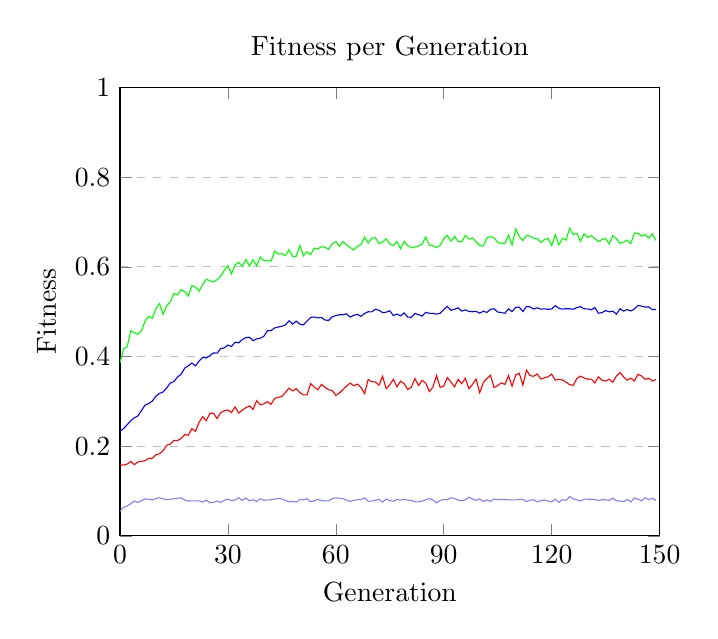
\begin{tikzpicture}
\begin{axis}[
	title={Fitness per Generation},
	xlabel={Generation},
	ylabel={Fitness},
	xmin=0, xmax=150,
	ymin=0, ymax=1,
	xtick={0.0,30.0,60.0,90.0,120.0,150.0},
	ytick={0.0,0.2,0.4,0.6000000000000001,0.8,1.0},
	ymajorgrids=true,
	grid style=dashed,
]

\addplot[
	color=green,
	]
	coordinates {
	(0,0.3854052380952381)(1,0.41743357142857146)(2,0.42157682539682534)(3,0.45713761904761896)(4,0.4532113492063491)(5,0.4495180158730159)(6,0.4580835714285714)(7,0.47940619047619054)(8,0.4897792857142858)(9,0.4855703968253968)(10,0.5073754761904762)(11,0.5182029365079365)(12,0.49415269841269843)(13,0.5134533333333333)(14,0.5221603174603175)(15,0.5406062698412699)(16,0.537418888888889)(17,0.5492764285714286)(18,0.5450616666666667)(19,0.5351248412698414)(20,0.5580815873015872)(21,0.554837619047619)(22,0.5460739682539683)(23,0.5606091269841271)(24,0.5724277777777779)(25,0.5690688095238096)(26,0.5665598412698412)(27,0.5714403174603174)(28,0.5791705555555555)(29,0.5925315873015873)(30,0.6027894444444445)(31,0.584477380952381)(32,0.6045595238095236)(33,0.6099875396825395)(34,0.6015640476190476)(35,0.6165365079365079)(36,0.601628015873016)(37,0.6159319841269841)(38,0.6024546031746031)(39,0.621714365079365)(40,0.614461746031746)(41,0.6140362698412697)(42,0.6129358730158728)(43,0.6350685714285714)(44,0.6287283333333332)(45,0.6293050793650794)(46,0.625271746031746)(47,0.6384260317460317)(48,0.622931507936508)(49,0.6238775396825398)(50,0.6476291269841271)(51,0.624780238095238)(52,0.6335662698412698)(53,0.6272449999999999)(54,0.6416805555555556)(55,0.6399261111111111)(56,0.6450772222222222)(57,0.6434280952380954)(58,0.639648253968254)(59,0.6516123809523808)(60,0.6563689682539684)(61,0.646167380952381)(62,0.6563975396825399)(63,0.6493376190476191)(64,0.6432475396825398)(65,0.6379366666666665)(66,0.6459992857142856)(67,0.6493377777777778)(68,0.6664628571428571)(69,0.6531426190476189)(70,0.6641951587301588)(71,0.6650793650793649)(72,0.6521000000000001)(73,0.6552315079365079)(74,0.6625942857142857)(75,0.6511775396825396)(76,0.6475480952380953)(77,0.6562457142857141)(78,0.6402173015873015)(79,0.656825)(80,0.6475980952380951)(81,0.6428030952380953)(82,0.644273492063492)(83,0.6467825396825397)(84,0.6511092063492065)(85,0.6663246825396826)(86,0.6482075396825396)(87,0.6470598412698413)(88,0.643404126984127)(89,0.648068650793651)(90,0.662906984126984)(91,0.6703600793650794)(92,0.6571707142857144)(93,0.6680363492063492)(94,0.6564643650793651)(95,0.6558188095238094)(96,0.6700690476190476)(97,0.6619723015873015)(98,0.6646146031746032)(99,0.6558840476190476)(100,0.6477884126984126)(101,0.646552380952381)(102,0.6645981746031745)(103,0.6676441269841268)(104,0.6647354761904762)(105,0.654767777777778)(106,0.6520855555555555)(107,0.6523888888888889)(108,0.6708454761904762)(109,0.649092380952381)(110,0.6844784126984128)(111,0.6677857936507936)(112,0.6587338888888888)(113,0.670345873015873)(114,0.6688483333333335)(115,0.6637397619047619)(116,0.663235)(117,0.6547445238095239)(118,0.6607136507936507)(119,0.6636344444444446)(120,0.6479490476190476)(121,0.671520238095238)(122,0.6490583333333333)(123,0.6639530952380952)(124,0.659686111111111)(125,0.6863349206349205)(126,0.6721211904761905)(127,0.6751194444444443)(128,0.6572322222222222)(129,0.6735532539682539)(130,0.6663234126984128)(131,0.6695684126984126)(132,0.6630360317460317)(133,0.6565759523809522)(134,0.6607265873015875)(135,0.6634681746031746)(136,0.6513348412698413)(137,0.6697131746031746)(138,0.6625357936507936)(139,0.6527003174603175)(140,0.655332619047619)(141,0.6596569047619047)(142,0.6520825396825396)(143,0.6752941269841268)(144,0.6749007936507937)(145,0.6685057142857143)(146,0.6720050793650794)(147,0.6644692857142858)(148,0.6735408730158731)(149,0.6590466666666667)
	};
\addplot[
	color=blue,
	]
	coordinates {
	(0,0.23341582010582007)(1,0.23945444444444444)(2,0.24783851851851849)(3,0.25716235119047626)(4,0.26332109788359787)(5,0.2677289186507937)(6,0.27987786375661383)(7,0.2918434656084656)(8,0.2950874107142857)(9,0.30078963955026455)(10,0.3117538624338625)(11,0.3178337202380953)(12,0.32097923941798945)(13,0.3303134788359788)(14,0.3408783333333334)(15,0.3442648544973545)(16,0.35423655423280426)(17,0.36054948743386245)(18,0.3741453207671957)(19,0.37947775793650795)(20,0.3856846428571429)(21,0.37914357473544974)(22,0.39005090277777776)(23,0.39806746362433865)(24,0.39679892857142857)(25,0.40206844246031753)(26,0.4080816236772486)(27,0.40757105489417994)(28,0.41777688822751324)(29,0.41939785714285716)(30,0.4256608399470899)(31,0.42226457671957673)(32,0.4319285251322752)(33,0.43078813161375656)(34,0.43775256613756613)(35,0.4422594113756613)(36,0.4430311342592593)(37,0.43540711309523805)(38,0.43943342592592594)(39,0.44099251653439153)(40,0.4451518882275132)(41,0.45763896825396816)(42,0.45787082671957674)(43,0.463810796957672)(44,0.4658672883597883)(45,0.4676191038359787)(46,0.4706087037037038)(47,0.47974581679894174)(48,0.47251104166666663)(49,0.4789437764550264)(50,0.47230957341269836)(51,0.47077102843915347)(52,0.47925345568783073)(53,0.48728440476190477)(54,0.4883141236772487)(55,0.4861945634920634)(56,0.4871138756613757)(57,0.4814951785714286)(58,0.48069697089947094)(59,0.4886677414021163)(60,0.4913268584656084)(61,0.49314797288359785)(62,0.49346536375661365)(63,0.49527057870370356)(64,0.48800184854497347)(65,0.4921009755291006)(66,0.49410188492063484)(67,0.4896091798941799)(68,0.49599869708994715)(69,0.4999505291005291)(70,0.4996031117724868)(71,0.5054025727513228)(72,0.5034298511904761)(73,0.49797306216931203)(74,0.49894483796296296)(75,0.5021025363756614)(76,0.4913355985449735)(77,0.4946915773809523)(78,0.49103020171957673)(79,0.49725307208994696)(80,0.48806354828042325)(81,0.48760354166666653)(82,0.496124083994709)(83,0.4935297255291005)(84,0.49025646164021164)(85,0.4986593022486772)(86,0.4963995072751324)(87,0.4964763624338623)(88,0.4946208697089947)(89,0.4965806481481483)(90,0.5047905886243387)(91,0.5119165542328042)(92,0.5031410879629629)(93,0.5056456746031748)(94,0.508678664021164)(95,0.5014229894179895)(96,0.5041261772486773)(97,0.5007670436507936)(98,0.49998588955026463)(99,0.5007977777777778)(100,0.4967750198412699)(101,0.501240052910053)(102,0.4984369841269841)(103,0.505365248015873)(104,0.506572833994709)(105,0.49940580687830693)(106,0.49813191798941786)(107,0.4964619146825397)(108,0.5063395403439154)(109,0.5003592328042328)(110,0.5095329133597883)(111,0.51022394510582)(112,0.5003574272486772)(113,0.5117254695767196)(114,0.5107324074074074)(115,0.5060257242063493)(116,0.5087623478835979)(117,0.5057140575396826)(118,0.5064873148148148)(119,0.5053898214285714)(120,0.5059754431216931)(121,0.5137332738095237)(122,0.5075575099206349)(123,0.5057553472222223)(124,0.5067626091269841)(125,0.5066025330687831)(126,0.5055479497354497)(127,0.5092545304232804)(128,0.5113969841269841)(129,0.5065815244708995)(130,0.5063532473544973)(131,0.5042983498677248)(132,0.5092361408730158)(133,0.49663533399470894)(134,0.49816279761904764)(135,0.502575009920635)(136,0.49977334325396816)(137,0.5012650396825398)(138,0.49470442460317465)(139,0.506419484126984)(140,0.5013479166666667)(141,0.5048558366402116)(142,0.501785906084656)(143,0.5060235085978837)(144,0.5141503604497355)(145,0.5124378339947091)(146,0.5103973842592593)(147,0.5105576190476191)(148,0.5047449933862435)(149,0.504938277116402)
	};
\addplot[
	color=red,
	]
	coordinates {
	(0,0.15805380952380957)(1,0.15798388888888887)(2,0.1600922222222222)(3,0.1661516666666667)(4,0.15895992063492068)(5,0.1649728571428571)(6,0.1662018253968254)(7,0.16789111111111116)(8,0.1730022222222222)(9,0.1731411904761904)(10,0.180869365079365)(11,0.1830757142857143)(12,0.19005547619047614)(13,0.20225960317460323)(14,0.2048926984126984)(15,0.21275087301587303)(16,0.21253507936507932)(17,0.21730158730158736)(18,0.22607301587301584)(19,0.22444111111111106)(20,0.23897722222222223)(21,0.23333412698412698)(22,0.2531914285714285)(23,0.2658061904761905)(24,0.25686841269841265)(25,0.27364341269841264)(26,0.2733891269841271)(27,0.2616154761904762)(28,0.2749590476190476)(29,0.27913999999999994)(30,0.2807914285714286)(31,0.27519325396825395)(32,0.28757698412698407)(33,0.2740437301587302)(34,0.28029531746031744)(35,0.2860158730158731)(36,0.2897703174603175)(37,0.28233206349206347)(38,0.30147007936507947)(39,0.2922761904761905)(40,0.29454888888888886)(41,0.29919079365079365)(42,0.2934353174603175)(43,0.3067492857142857)(44,0.3088384126984126)(45,0.3109788888888889)(46,0.32013222222222226)(47,0.32943873015873026)(48,0.32345206349206335)(49,0.32843555555555565)(50,0.31969484126984116)(51,0.3146953968253968)(52,0.3144192063492063)(53,0.3396014285714285)(54,0.3318397619047619)(55,0.3259561111111111)(56,0.33786555555555564)(57,0.331658253968254)(58,0.325785873015873)(59,0.32466817460317454)(60,0.31344333333333335)(61,0.31860079365079363)(62,0.3263800793650794)(63,0.33395619047619046)(64,0.3407312698412698)(65,0.3347949206349207)(66,0.3385203174603174)(67,0.3310021428571429)(68,0.3174053968253968)(69,0.3488382539682539)(70,0.34395785714285715)(71,0.3433549206349207)(72,0.3361536507936508)(73,0.35592753968253965)(74,0.3285948412698413)(75,0.33709968253968253)(76,0.34920444444444443)(77,0.33255388888888887)(78,0.345180634920635)(79,0.33964055555555556)(80,0.3267117460317461)(81,0.3320415873015872)(82,0.3509279365079366)(83,0.3355633333333333)(84,0.3468884126984126)(85,0.3403057142857143)(86,0.32206579365079374)(87,0.3319703968253968)(88,0.3575314285714285)(89,0.33117761904761905)(90,0.3340311111111111)(91,0.3531091269841271)(92,0.34308238095238086)(93,0.3326664285714286)(94,0.3491501587301588)(95,0.339572619047619)(96,0.35145912698412696)(97,0.3284585714285715)(98,0.3381631746031745)(99,0.34999960317460316)(100,0.3194007936507937)(101,0.3419467460317461)(102,0.3511061111111111)(103,0.35817277777777773)(104,0.3308245238095238)(105,0.335285238095238)(106,0.3412398412698412)(107,0.33795277777777766)(108,0.35746373015873023)(109,0.3341884126984127)(110,0.35890785714285717)(111,0.3628196031746031)(112,0.33637103174603167)(113,0.36962071428571425)(114,0.35739984126984137)(115,0.3560751587301589)(116,0.36113031746031743)(117,0.3500217460317461)(118,0.3526938095238096)(119,0.3548763492063492)(120,0.36088174603174605)(121,0.3473142857142857)(122,0.34891865079365086)(123,0.34780952380952385)(124,0.34295690476190477)(125,0.33752103174603176)(126,0.33578674603174613)(127,0.35104507936507934)(128,0.35616952380952377)(129,0.35252301587301593)(130,0.34935190476190475)(131,0.3496787301587301)(132,0.3412313492063492)(133,0.3547953174603174)(134,0.347195873015873)(135,0.34561063492063493)(136,0.3492407142857142)(137,0.34286984126984127)(138,0.3566372222222223)(139,0.3643493650793651)(140,0.35451674603174615)(141,0.3472307936507937)(142,0.35183420634920637)(143,0.34557119047619045)(144,0.36032587301587304)(145,0.35661388888888895)(146,0.34930944444444445)(147,0.35150301587301586)(148,0.3455242063492063)(149,0.3489911904761905)
	};
\addplot[
	color=blue!50,
	]
	coordinates {
	(0,0.054901299845547605)(1,0.06411441249312055)(2,0.06655982056205524)(3,0.07199652265558798)(4,0.07785960977008408)(5,0.07448264641256473)(6,0.07910181082758984)(7,0.08236876444110477)(8,0.08175827540129947)(9,0.08026704656290362)(10,0.0831185299234548)(11,0.08511072867000284)(12,0.08253824178237378)(13,0.08069349543430203)(14,0.08158794474895853)(15,0.08285722979572434)(16,0.08415884788466033)(17,0.08470794426449926)(18,0.08014437372039765)(19,0.07779969071434409)(20,0.07806765013153726)(21,0.07823211490716238)(22,0.07798909624865565)(23,0.07536941280902942)(24,0.0798927974789094)(25,0.07387577854073507)(26,0.07459046010935125)(27,0.07776552146968749)(28,0.07471112099933166)(29,0.0794060734484023)(30,0.08206579060771275)(31,0.07860883069026822)(32,0.07997651316142897)(33,0.08509363382668063)(34,0.07883909262012584)(35,0.08445866751671213)(36,0.07801111482461398)(37,0.08062531923572895)(38,0.07678200341002733)(39,0.08243369007948574)(40,0.07947808498061511)(41,0.08040287843804053)(42,0.08051403797774363)(43,0.08207704515006604)(44,0.08373122552630786)(45,0.08230673127600444)(46,0.07929054592274597)(47,0.07598493411098428)(48,0.0767676027066942)(49,0.0754316771467542)(50,0.08126417832820812)(51,0.0802877365396467)(52,0.08287528317515519)(53,0.07597595231473361)(54,0.07828561343893967)(55,0.08128943354289052)(56,0.07891823630850497)(57,0.0781378786552582)(58,0.07819997712559311)(59,0.0832372862600825)(60,0.08480495762503225)(61,0.08412315043243616)(62,0.08275863768476331)(63,0.08011512743399074)(64,0.07672043392543922)(65,0.07949971532020567)(66,0.08059741265679057)(67,0.0810988950378033)(68,0.08473379607261049)(69,0.07734776020400012)(70,0.07761647464907029)(71,0.07940917382752717)(72,0.08147429787022571)(73,0.07499777186328274)(74,0.08245526035034005)(75,0.07866269358576122)(76,0.07724554044985779)(77,0.08130452827373005)(78,0.07965027484469396)(79,0.08174042721877514)(80,0.07973370191107185)(81,0.07931816658441587)(82,0.07581976391220452)(83,0.07598149724379231)(84,0.07745070549187023)(85,0.08055296329685892)(86,0.08301905532779191)(87,0.08042208071164476)(88,0.07364336573176647)(89,0.07904528804428837)(90,0.08115463500532287)(91,0.08036678000639456)(92,0.08521510854287626)(93,0.08313050739357976)(94,0.07968652513752095)(95,0.07881087292583264)(96,0.08031305482629213)(97,0.08608792563659728)(98,0.08216663099061844)(99,0.07935819957297928)(100,0.08249752183415829)(101,0.07684604623791752)(102,0.08014567273685397)(103,0.07728960611293927)(104,0.0820591455461682)(105,0.08097046920979523)(106,0.08161484464809739)(107,0.08107212105821088)(108,0.08038419511118307)(109,0.08024534762082762)(110,0.0802296561095919)(111,0.08131895116959786)(112,0.08142293603587103)(113,0.07669717192544961)(114,0.07970129742358989)(115,0.08048550581089028)(116,0.07584218701935354)(117,0.07876050190014527)(118,0.08015475690175417)(119,0.07775114064561323)(120,0.0756766742276645)(121,0.08177976514340028)(122,0.07483010082813475)(123,0.08105791712535086)(124,0.07924585758478042)(125,0.08779714954179542)(126,0.08268689561129135)(127,0.08074621022209912)(128,0.07781683823667666)(129,0.08183925493647207)(130,0.08188356559396069)(131,0.081469382717169)(132,0.08105927808404978)(133,0.0790191543877171)(134,0.0806126206984968)(135,0.08046559869872327)(136,0.0792349257157087)(137,0.0843099756511807)(138,0.07829753798354902)(139,0.0776950892313251)(140,0.07662964252015908)(141,0.08119862365834848)(142,0.0756914918749451)(143,0.08475610167240939)(144,0.08183239889228806)(145,0.07835718056821717)(146,0.08485622720402053)(147,0.08084384975864646)(148,0.08415944598028657)(149,0.0789308387006915)
	};
\end{axis}
\end{tikzpicture}
}
		\caption{Some sample caption}
	\end{subfigure}%
	
	
}
\caption{Figure shows results from a simulation in the easy environment (p.1)}
\end{figure}

\newpage
\vspace*{-2.0cm}
\textbf{\Huge Results -  Easy environment (2) }
\vspace{1.5cm}
\begin{tikzpicture}[remember picture,overlay]
   \node[anchor=south east,inner sep=20pt] at (current page.south east)
              {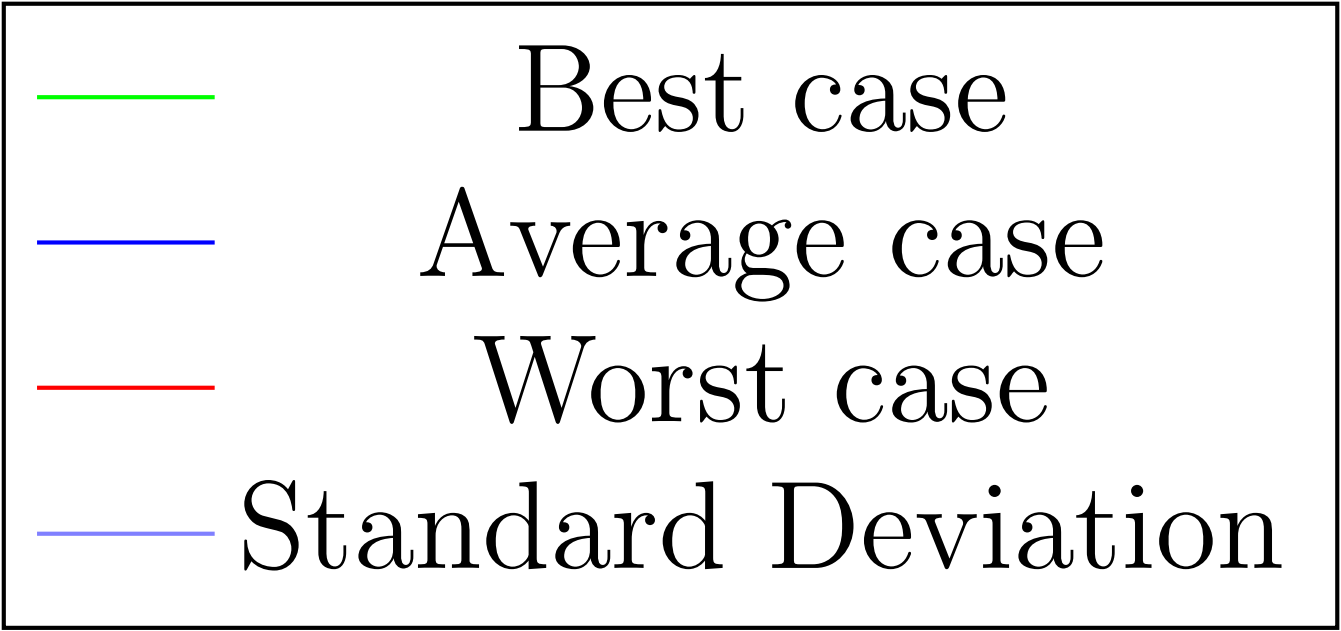
\includegraphics[scale=0.1]{chapters/res/generated_graph_legend.png}};
\end{tikzpicture}

\begin{figure}[H]
\vspace*{-1cm}
	\makebox[\linewidth][c]{%
	\begin{subfigure}[b]{0.7\textwidth}
		\centering
		\resizebox{0.9\linewidth}{!}{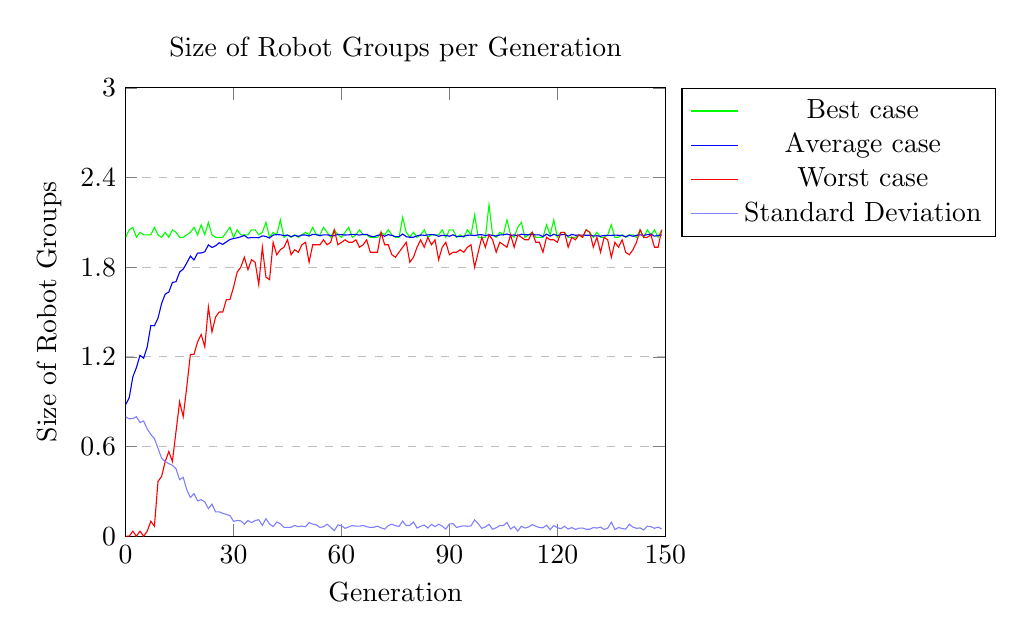
\begin{tikzpicture}
\begin{axis}[
	title={Size of Robot Groups per Generation},
	xlabel={Generation},
	ylabel={Size of Robot Groups},
	xmin=0, xmax=150,
	ymin=0, ymax=3,
	xtick={0.0,30.0,60.0,90.0,120.0,150.0},
	ytick={0.0,0.6,1.2,1.7999999999999998,2.4,3.0},
	legend pos=outer north east,
	ymajorgrids=true,
	grid style=dashed,
]

\addplot[
	color=green,
	]
	coordinates {
	(0,2.0000000000000004)(1,2.0500000000000003)(2,2.0666666666666673)(3,2.0000000000000004)(4,2.033333333333334)(5,2.016666666666667)(6,2.016666666666667)(7,2.0166666666666675)(8,2.0666666666666673)(9,2.016666666666667)(10,2.0000000000000004)(11,2.033333333333334)(12,2.0000000000000004)(13,2.0500000000000007)(14,2.0333333333333337)(15,2.0000000000000004)(16,2.0000000000000004)(17,2.0166666666666675)(18,2.033333333333334)(19,2.0666666666666673)(20,2.016666666666667)(21,2.083333333333334)(22,2.016666666666667)(23,2.1)(24,2.0166666666666675)(25,2.0000000000000004)(26,2.0000000000000004)(27,2.0000000000000004)(28,2.033333333333334)(29,2.0666666666666673)(30,2.0000000000000004)(31,2.0500000000000007)(32,2.016666666666667)(33,2.0166666666666675)(34,2.016666666666667)(35,2.0500000000000007)(36,2.0500000000000003)(37,2.016666666666667)(38,2.033333333333334)(39,2.100000000000001)(40,2.0000000000000004)(41,2.0333333333333337)(42,2.016666666666667)(43,2.116666666666667)(44,2.0000000000000004)(45,2.0166666666666675)(46,2.0000000000000004)(47,2.016666666666667)(48,2.0000000000000004)(49,2.0166666666666675)(50,2.033333333333334)(51,2.016666666666667)(52,2.0666666666666673)(53,2.016666666666667)(54,2.0166666666666675)(55,2.0666666666666673)(56,2.033333333333334)(57,2.0000000000000004)(58,2.0500000000000007)(59,2.016666666666667)(60,2.0000000000000004)(61,2.033333333333334)(62,2.0666666666666673)(63,2.0000000000000004)(64,2.0166666666666675)(65,2.0500000000000003)(66,2.0166666666666675)(67,2.016666666666667)(68,2.0000000000000004)(69,2.0000000000000004)(70,2.0000000000000004)(71,2.033333333333334)(72,2.016666666666667)(73,2.0500000000000007)(74,2.0166666666666675)(75,2.0000000000000004)(76,2.0000000000000004)(77,2.1333333333333337)(78,2.033333333333334)(79,2.0000000000000004)(80,2.033333333333334)(81,2.0000000000000004)(82,2.0166666666666675)(83,2.0500000000000003)(84,2.0000000000000004)(85,2.0166666666666675)(86,2.016666666666667)(87,2.016666666666667)(88,2.0500000000000007)(89,2.0000000000000004)(90,2.0500000000000007)(91,2.0500000000000007)(92,2.0000000000000004)(93,2.016666666666667)(94,2.0000000000000004)(95,2.0500000000000003)(96,2.016666666666667)(97,2.150000000000001)(98,2.0000000000000004)(99,2.0000000000000004)(100,2.0000000000000004)(101,2.216666666666667)(102,2.0166666666666675)(103,2.0000000000000004)(104,2.033333333333334)(105,2.0166666666666675)(106,2.1166666666666676)(107,2.0166666666666675)(108,2.0000000000000004)(109,2.0666666666666673)(110,2.1)(111,2.0000000000000004)(112,2.0166666666666675)(113,2.033333333333334)(114,2.0000000000000004)(115,2.0000000000000004)(116,2.0000000000000004)(117,2.0833333333333344)(118,2.0166666666666675)(119,2.1166666666666676)(120,2.0000000000000004)(121,2.033333333333334)(122,2.033333333333334)(123,2.0000000000000004)(124,2.0000000000000004)(125,2.0000000000000004)(126,2.016666666666667)(127,2.0000000000000004)(128,2.0500000000000007)(129,2.033333333333334)(130,2.0000000000000004)(131,2.033333333333334)(132,2.0000000000000004)(133,2.0000000000000004)(134,2.0166666666666675)(135,2.083333333333334)(136,2.0000000000000004)(137,2.0000000000000004)(138,2.016666666666667)(139,2.0000000000000004)(140,2.0166666666666675)(141,2.016666666666667)(142,2.0000000000000004)(143,2.0500000000000007)(144,2.0000000000000004)(145,2.0500000000000007)(146,2.016666666666667)(147,2.0500000000000003)(148,2.0000000000000004)(149,2.0500000000000007)
	};
	\addlegendentry{Best case}
\addplot[
	color=blue,
	]
	coordinates {
	(0,0.8798611111111109)(1,0.9270833333333335)(2,1.065972222222222)(3,1.1284722222222223)(4,1.2104166666666665)(5,1.190972222222222)(6,1.2666666666666666)(7,1.4097222222222223)(8,1.4083333333333334)(9,1.4590277777777778)(10,1.5576388888888886)(11,1.6201388888888886)(12,1.6333333333333335)(13,1.697916666666667)(14,1.7027777777777782)(15,1.7673611111111112)(16,1.7868055555555558)(17,1.8291666666666666)(18,1.8743055555555561)(19,1.8486111111111116)(20,1.8944444444444448)(21,1.8951388888888892)(22,1.9034722222222227)(23,1.9493055555555558)(24,1.9319444444444447)(25,1.943055555555556)(26,1.9631944444444447)(27,1.9527777777777782)(28,1.9694444444444448)(29,1.9854166666666675)(30,1.991666666666667)(31,1.9965277777777781)(32,2.0034722222222223)(33,2.013194444444445)(34,1.995138888888889)(35,1.9986111111111116)(36,1.9979166666666666)(37,1.9972222222222227)(38,2.0097222222222224)(39,2.005555555555556)(40,1.9951388888888892)(41,2.015277777777778)(42,2.0180555555555557)(43,2.016666666666667)(44,2.0125000000000006)(45,2.0145833333333334)(46,2.0041666666666673)(47,2.0131944444444447)(48,2.0062500000000005)(49,2.0152777777777784)(50,2.0152777777777784)(51,2.009027777777778)(52,2.019444444444445)(53,2.018055555555556)(54,2.010416666666667)(55,2.016666666666667)(56,2.016666666666667)(57,2.0118055555555556)(58,2.010416666666667)(59,2.0201388888888894)(60,2.0173611111111116)(61,2.0152777777777784)(62,2.016666666666667)(63,2.019444444444445)(64,2.0187500000000003)(65,2.014583333333334)(66,2.0201388888888894)(67,2.019444444444445)(68,2.0083333333333337)(69,2.0034722222222228)(70,2.0131944444444447)(71,2.017361111111111)(72,2.0069444444444446)(73,2.018055555555556)(74,2.0125000000000006)(75,2.0048611111111114)(76,2.0048611111111114)(77,2.0222222222222226)(78,2.0041666666666673)(79,2.0000000000000004)(80,2.0006944444444446)(81,2.0097222222222224)(82,2.0159722222222225)(83,2.013194444444445)(84,2.0159722222222225)(85,2.0187500000000003)(86,2.0159722222222225)(87,2.0069444444444446)(88,2.0131944444444447)(89,2.0131944444444447)(90,2.0069444444444446)(91,2.016666666666667)(92,2.005555555555556)(93,2.005555555555556)(94,2.0069444444444446)(95,2.0138888888888893)(96,2.0145833333333334)(97,2.0118055555555556)(98,2.016666666666667)(99,2.0173611111111116)(100,2.0111111111111115)(101,2.017361111111111)(102,2.0125000000000006)(103,2.0083333333333337)(104,2.0159722222222225)(105,2.016666666666667)(106,2.0222222222222226)(107,2.013194444444445)(108,2.0159722222222225)(109,2.0111111111111115)(110,2.020833333333334)(111,2.0173611111111116)(112,2.016666666666667)(113,2.0208333333333335)(114,2.015972222222223)(115,2.0159722222222225)(116,2.0048611111111114)(117,2.020833333333334)(118,2.007638888888889)(119,2.0201388888888894)(120,2.0118055555555556)(121,2.016666666666667)(122,2.020138888888889)(123,2.007638888888889)(124,2.0194444444444453)(125,2.0138888888888893)(126,2.014583333333334)(127,2.0145833333333334)(128,2.0138888888888893)(129,2.013888888888889)(130,2.009027777777778)(131,2.010416666666667)(132,2.006944444444445)(133,2.0131944444444447)(134,2.0125000000000006)(135,2.0131944444444447)(136,2.014583333333334)(137,2.0138888888888893)(138,2.0118055555555556)(139,2.0041666666666673)(140,2.013888888888889)(141,2.006944444444445)(142,2.013194444444445)(143,2.016666666666667)(144,2.0125000000000006)(145,2.0180555555555557)(146,2.021527777777778)(147,2.007638888888889)(148,2.0125)(149,2.0159722222222225)
	};
	\addlegendentry{Average case}
\addplot[
	color=red,
	]
	coordinates {
	(0,0.0)(1,0.0)(2,0.03333333333333333)(3,0.0)(4,0.03333333333333333)(5,0.0)(6,0.03333333333333333)(7,0.1)(8,0.06666666666666667)(9,0.3666666666666667)(10,0.4)(11,0.49999999999999994)(12,0.5666666666666667)(13,0.5)(14,0.7)(15,0.8999999999999999)(16,0.7999999999999999)(17,0.9999999999999999)(18,1.2166666666666668)(19,1.2166666666666668)(20,1.3)(21,1.35)(22,1.2666666666666666)(23,1.5333333333333334)(24,1.3666666666666667)(25,1.4666666666666668)(26,1.5000000000000002)(27,1.5000000000000002)(28,1.5833333333333337)(29,1.5833333333333335)(30,1.666666666666667)(31,1.766666666666667)(32,1.8000000000000005)(33,1.8666666666666671)(34,1.7833333333333339)(35,1.8500000000000008)(36,1.833333333333334)(37,1.6833333333333336)(38,1.9333333333333338)(39,1.7333333333333338)(40,1.716666666666667)(41,1.9666666666666672)(42,1.8833333333333337)(43,1.9166666666666672)(44,1.933333333333334)(45,1.983333333333334)(46,1.883333333333334)(47,1.9166666666666672)(48,1.9000000000000006)(49,1.9500000000000006)(50,1.9666666666666672)(51,1.833333333333334)(52,1.9500000000000006)(53,1.9500000000000006)(54,1.9500000000000006)(55,1.983333333333334)(56,1.9500000000000006)(57,1.9666666666666675)(58,2.0500000000000007)(59,1.9500000000000006)(60,1.9666666666666675)(61,1.983333333333334)(62,1.9666666666666675)(63,1.9666666666666672)(64,1.983333333333334)(65,1.933333333333334)(66,1.9500000000000006)(67,1.983333333333334)(68,1.9000000000000006)(69,1.9000000000000006)(70,1.9000000000000004)(71,2.033333333333334)(72,1.9500000000000004)(73,1.9500000000000006)(74,1.883333333333334)(75,1.8666666666666671)(76,1.9000000000000008)(77,1.9333333333333342)(78,1.9666666666666675)(79,1.833333333333334)(80,1.8666666666666674)(81,1.933333333333334)(82,1.983333333333334)(83,1.9333333333333338)(84,2.0000000000000004)(85,1.9500000000000008)(86,1.983333333333334)(87,1.8500000000000003)(88,1.9333333333333338)(89,1.9666666666666672)(90,1.883333333333334)(91,1.9000000000000006)(92,1.9000000000000006)(93,1.9166666666666672)(94,1.9000000000000004)(95,1.933333333333334)(96,1.9500000000000004)(97,1.8000000000000005)(98,1.9000000000000006)(99,2.0000000000000004)(100,1.933333333333334)(101,2.016666666666667)(102,1.983333333333334)(103,1.9000000000000006)(104,1.9666666666666672)(105,1.9500000000000006)(106,1.933333333333334)(107,2.0166666666666675)(108,1.933333333333334)(109,2.016666666666667)(110,2.0000000000000004)(111,1.9833333333333338)(112,1.983333333333334)(113,2.033333333333334)(114,1.9666666666666675)(115,1.9666666666666672)(116,1.9000000000000008)(117,2.000000000000001)(118,1.983333333333334)(119,1.983333333333334)(120,1.9666666666666672)(121,2.033333333333334)(122,2.033333333333334)(123,1.933333333333334)(124,2.0000000000000004)(125,1.983333333333334)(126,2.016666666666667)(127,2.0000000000000004)(128,2.0500000000000007)(129,2.033333333333334)(130,1.933333333333334)(131,2.0000000000000004)(132,1.9000000000000006)(133,2.0000000000000004)(134,1.983333333333334)(135,1.8666666666666671)(136,1.9666666666666672)(137,1.933333333333334)(138,1.983333333333334)(139,1.9000000000000006)(140,1.883333333333334)(141,1.9166666666666672)(142,1.9666666666666672)(143,2.0500000000000007)(144,2.0000000000000004)(145,2.0000000000000004)(146,2.016666666666667)(147,1.933333333333334)(148,1.9333333333333338)(149,2.0500000000000007)
	};
	\addlegendentry{Worst case}
\addplot[
	color=blue!50,
	]
	coordinates {
	(0,0.7983311755495729)(1,0.7855423863953697)(2,0.7871253815576873)(3,0.7993947144540696)(4,0.7607876356614588)(5,0.771121278903698)(6,0.7173637423564808)(7,0.6805657166864519)(8,0.6536032240985181)(9,0.5881336499750809)(10,0.522056049245939)(11,0.498929027559466)(12,0.4858452636748676)(13,0.47426272476363873)(14,0.4513992046882054)(15,0.3783832537381997)(16,0.39384225446691024)(17,0.31048799645347164)(18,0.2590721203711587)(19,0.28441688256920156)(20,0.2363118528974239)(21,0.24450045613956498)(22,0.22899622710176998)(23,0.18444716314296203)(24,0.21439099799215794)(25,0.16250380986475277)(26,0.16288251381517108)(27,0.1525886568336205)(28,0.1461005948903228)(29,0.13774057959377478)(30,0.09935192773515408)(31,0.10506597780370139)(32,0.10271112307798994)(33,0.08070167915624644)(34,0.1049299510813909)(35,0.09080447963431791)(36,0.10483896386180852)(37,0.11018124736037944)(38,0.07233578380873369)(39,0.1172302362616263)(40,0.08175385336604217)(41,0.06407846802894583)(42,0.09452894622226322)(43,0.08388685928532247)(44,0.05895403092354805)(45,0.05861265956460498)(46,0.05994685633484004)(47,0.07195681098401753)(48,0.06393733203827232)(49,0.06737496015590203)(50,0.06359759902837278)(51,0.09101916664136402)(52,0.08115267548306442)(53,0.07609174654563443)(54,0.058076558300094255)(55,0.0635479747400224)(56,0.08023636355558941)(57,0.059296514552138094)(58,0.03697210013558607)(59,0.07549963892319081)(60,0.06970398860378861)(61,0.0525757399972869)(62,0.062197966765405406)(63,0.07081355584902373)(64,0.06746860557348561)(65,0.06697142609279465)(66,0.07231793396942153)(67,0.06327185523854088)(68,0.05818149233540158)(69,0.0602275734107459)(70,0.06669822649965446)(71,0.056140135218514034)(72,0.04695352688510336)(73,0.07126311549110305)(74,0.07998629605061357)(75,0.07080336741015113)(76,0.06519777057108839)(77,0.10077294522411565)(78,0.070921009470098)(79,0.07273177330726799)(80,0.09534162990198641)(81,0.05433621068542154)(82,0.06677302050007788)(83,0.07455005537166758)(84,0.054564230976556626)(85,0.07920427313409775)(86,0.06376971228479242)(87,0.07984576369931783)(88,0.0667604519691524)(89,0.04775001047577603)(90,0.08185074402210286)(91,0.08377458885323448)(92,0.058239451988007646)(93,0.06481755528041662)(94,0.06942397860035467)(95,0.06654046261217178)(96,0.06883183128967238)(97,0.10901646668949469)(98,0.083468000038766)(99,0.05260108809622554)(100,0.06239267530067373)(101,0.07940802265262764)(102,0.046699935379844626)(103,0.05635761222544963)(104,0.07081058878460422)(105,0.07122368479476444)(106,0.09199269193524985)(107,0.04790629418434261)(108,0.06511086041378902)(109,0.03393267338885214)(110,0.06678030073406985)(111,0.05430261734104916)(112,0.06188929379003112)(113,0.07706023784286557)(114,0.06685709526773043)(115,0.057518442950805874)(116,0.05613733780994192)(117,0.07363665914908524)(118,0.043793216980518676)(119,0.0710549004894864)(120,0.05687163457239522)(121,0.05048831357126835)(122,0.06627967438396375)(123,0.048095556230850454)(124,0.057559415354062865)(125,0.04548610419268803)(126,0.05358149285733128)(127,0.0545671713000547)(128,0.04642112856009753)(129,0.04663698225927933)(130,0.05764983499075631)(131,0.05438977845065981)(132,0.061140232585419174)(133,0.045116171422411554)(134,0.05391038471281062)(135,0.09401177183242798)(136,0.044812624133544074)(137,0.05805463242722705)(138,0.051609393535579466)(139,0.04732865859134238)(140,0.07987567175003345)(141,0.0608128956302697)(142,0.052761489495149756)(143,0.05527316217652164)(144,0.04194473510807866)(145,0.0666473349355931)(146,0.06382806510689948)(147,0.052632647136887735)(148,0.061008484719322104)(149,0.04807421234316709)
	};
	\addlegendentry{Standard Deviation}
\end{axis}
\end{tikzpicture}
}
		\caption{Some sample caption}
	\end{subfigure}%
	\begin{subfigure}[b]{0.7\textwidth}
		\centering
		\resizebox{0.9\linewidth}{!}{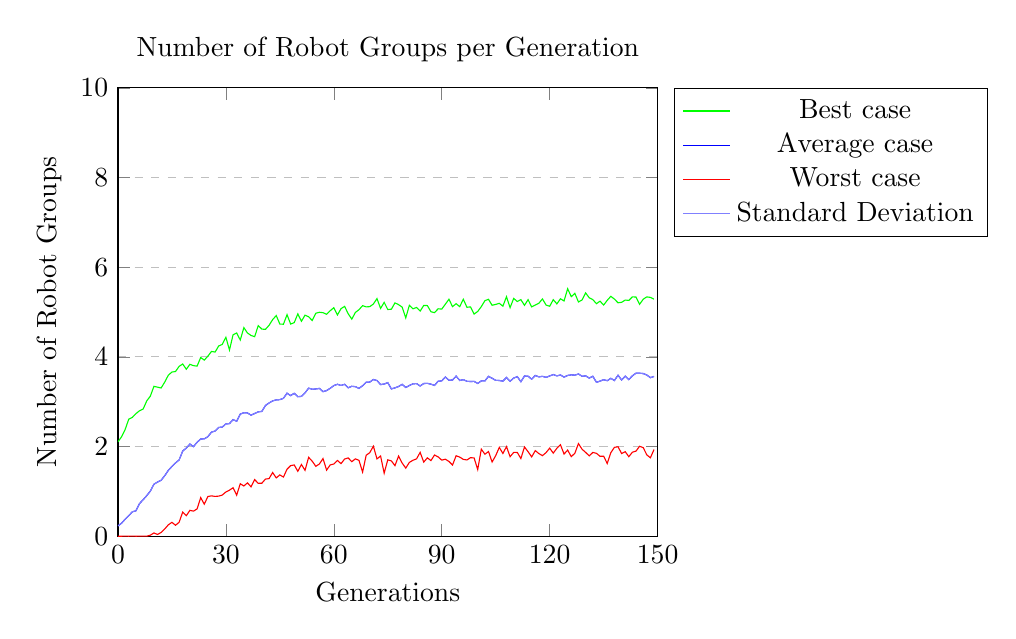
\begin{tikzpicture}
\begin{axis}[
	title={Number of Robot Groups per Generation},
	xlabel={Generations},
	ylabel={Number of Robot Groups},
	xmin=0, xmax=150,
	ymin=0, ymax=10,
	xtick={0.0,30.0,60.0,90.0,120.0,150.0},
	ytick={0.0,2.0,4.0,6.0,8.0,10.0},
	legend pos=outer north east,
	ymajorgrids=true,
	grid style=dashed,
]

\addplot[
	color=green,
	]
	coordinates {
	(0,2.103833333333333)(1,2.216666666666667)(2,2.3800833333333333)(3,2.6098333333333326)(4,2.6499166666666665)(5,2.7333333333333343)(6,2.7982499999999995)(7,2.8364166666666666)(8,3.017083333333333)(9,3.1240000000000006)(10,3.342416666666667)(11,3.324916666666666)(12,3.305166666666667)(13,3.4375833333333334)(14,3.5911666666666675)(15,3.66125)(16,3.6731666666666665)(17,3.7879166666666673)(18,3.8410833333333327)(19,3.723999999999999)(20,3.833333333333333)(21,3.8041666666666663)(22,3.793333333333334)(23,3.9860833333333336)(24,3.927666666666667)(25,4.016333333333334)(26,4.121333333333333)(27,4.106750000000001)(28,4.242916666666666)(29,4.2780000000000005)(30,4.437916666666666)(31,4.15275)(32,4.493583333333333)(33,4.5334166666666675)(34,4.375583333333333)(35,4.652416666666667)(36,4.533)(37,4.476916666666666)(38,4.4505)(39,4.698250000000001)(40,4.618916666666667)(41,4.6137500000000005)(42,4.703416666666666)(43,4.830666666666667)(44,4.92175)(45,4.73125)(46,4.727916666666668)(47,4.941166666666667)(48,4.732)(49,4.764083333333333)(50,4.9588333333333345)(51,4.793916666666665)(52,4.93)(53,4.894833333333334)(54,4.8105)(55,4.973083333333333)(56,4.9946666666666655)(57,4.985666666666667)(58,4.949416666666667)(59,5.0295)(60,5.096916666666667)(61,4.933249999999999)(62,5.074750000000002)(63,5.126500000000001)(64,4.9615833333333335)(65,4.842083333333333)(66,4.990583333333333)(67,5.052583333333333)(68,5.1418333333333335)(69,5.1152500000000005)(70,5.119999999999999)(71,5.179666666666667)(72,5.299416666666666)(73,5.080666666666666)(74,5.21575)(75,5.055833333333333)(76,5.063583333333333)(77,5.204416666666668)(78,5.165333333333334)(79,5.1098333333333334)(80,4.868416666666666)(81,5.149500000000001)(82,5.071250000000001)(83,5.102166666666666)(84,5.021166666666668)(85,5.146583333333332)(86,5.144500000000001)(87,5.006916666666667)(88,4.986083333333333)(89,5.07275)(90,5.064916666666666)(91,5.174499999999999)(92,5.285)(93,5.12075)(94,5.186333333333333)(95,5.120583333333334)(96,5.285416666666667)(97,5.106416666666667)(98,5.115500000000001)(99,4.954916666666665)(100,5.01225)(101,5.121000000000001)(102,5.2535)(103,5.284333333333334)(104,5.150916666666667)(105,5.169999999999999)(106,5.194166666666666)(107,5.131416666666667)(108,5.341666666666668)(109,5.098000000000001)(110,5.303833333333333)(111,5.235166666666667)(112,5.276083333333332)(113,5.150333333333332)(114,5.2763333333333335)(115,5.1146666666666665)(116,5.1570833333333335)(117,5.195749999999999)(118,5.292583333333334)(119,5.155916666666666)(120,5.127916666666668)(121,5.27575)(122,5.181750000000001)(123,5.2950833333333325)(124,5.2475000000000005)(125,5.520000000000001)(126,5.3421666666666665)(127,5.417333333333334)(128,5.22425)(129,5.269416666666666)(130,5.426500000000001)(131,5.317749999999999)(132,5.276916666666668)(133,5.186666666666666)(134,5.2420833333333325)(135,5.1555833333333325)(136,5.26075)(137,5.351083333333333)(138,5.287999999999999)(139,5.206999999999999)(140,5.2165)(141,5.267250000000001)(142,5.258666666666667)(143,5.3382499999999995)(144,5.334666666666666)(145,5.1725)(146,5.285583333333334)(147,5.337916666666667)(148,5.3265)(149,5.287083333333333)
	};
	\addlegendentry{Best case}
\addplot[
	color=blue,
	]
	coordinates {
	(0,0.22944444444444445)(1,0.2897256944444444)(2,0.3776875)(3,0.45748263888888885)(4,0.5443437499999999)(5,0.5652222222222223)(6,0.7281284722222222)(7,0.8133958333333332)(8,0.9048298611111111)(9,1.0064652777777778)(10,1.1595208333333333)(11,1.20740625)(12,1.2472430555555558)(13,1.3494340277777779)(14,1.4696145833333332)(15,1.5540312499999998)(16,1.6347048611111112)(17,1.7002013888888887)(18,1.9000243055555552)(19,1.9661909722222215)(20,2.055034722222222)(21,1.9968229166666667)(22,2.0951319444444447)(23,2.1680451388888886)(24,2.1707083333333337)(25,2.220381944444444)(26,2.3215555555555563)(27,2.34546875)(28,2.42478125)(29,2.4347499999999997)(30,2.504520833333333)(31,2.511840277777778)(32,2.600440972222223)(33,2.5641805555555552)(34,2.7248159722222227)(35,2.753475694444445)(36,2.749263888888889)(37,2.699975694444445)(38,2.7366666666666664)(39,2.7738472222222224)(40,2.7836388888888886)(41,2.914875)(42,2.971628472222222)(43,3.0177013888888884)(44,3.040899305555555)(45,3.0462638888888893)(46,3.0754062499999995)(47,3.1897847222222224)(48,3.135729166666667)(49,3.1878090277777784)(50,3.111611111111111)(51,3.1188611111111113)(52,3.195375)(53,3.3019270833333327)(54,3.2778888888888877)(55,3.2840381944444443)(56,3.2968854166666666)(57,3.2238750000000005)(58,3.2483749999999993)(59,3.2988854166666663)(60,3.359409722222222)(61,3.3888368055555556)(62,3.3633055555555544)(63,3.3872986111111114)(64,3.310559027777778)(65,3.343572916666667)(66,3.3356597222222226)(67,3.2969131944444445)(68,3.3565069444444444)(69,3.4367465277777773)(70,3.4385138888888886)(71,3.4944444444444454)(72,3.4721215277777775)(73,3.381340277777778)(74,3.3942430555555547)(75,3.4257395833333337)(76,3.285527777777778)(77,3.3085208333333336)(78,3.3395347222222225)(79,3.386673611111111)(80,3.317909722222223)(81,3.360357638888889)(82,3.399354166666667)(83,3.403611111111111)(84,3.351138888888888)(85,3.4049895833333332)(86,3.410024305555556)(87,3.3914375000000003)(88,3.363243055555556)(89,3.456694444444444)(90,3.464361111111111)(91,3.5504583333333333)(92,3.479260416666666)(93,3.4847847222222224)(94,3.570934027777777)(95,3.473482638888888)(96,3.49190625)(97,3.455409722222222)(98,3.4501562499999996)(99,3.4527673611111114)(100,3.407545138888889)(101,3.4642152777777775)(102,3.4629930555555557)(103,3.5658090277777776)(104,3.5228090277777775)(105,3.4762881944444444)(106,3.473281250000001)(107,3.458930555555556)(108,3.5397361111111114)(109,3.456211805555555)(110,3.526486111111111)(111,3.5589861111111114)(112,3.4459375000000003)(113,3.5729270833333326)(114,3.569180555555555)(115,3.501447916666667)(116,3.5862013888888895)(117,3.5537916666666667)(118,3.565930555555556)(119,3.5427569444444442)(120,3.573777777777778)(121,3.605694444444445)(122,3.575979166666667)(123,3.595725694444444)(124,3.5488923611111107)(125,3.585704861111111)(126,3.5982222222222227)(127,3.5927708333333337)(128,3.6184236111111123)(129,3.5678958333333335)(130,3.5761909722222223)(131,3.5271249999999994)(132,3.5677812500000003)(133,3.4326111111111115)(134,3.4602361111111106)(135,3.4899444444444447)(136,3.4688472222222217)(137,3.5216875)(138,3.4723472222222225)(139,3.590329861111111)(140,3.483791666666667)(141,3.5689027777777773)(142,3.4936805555555557)(143,3.5777569444444453)(144,3.635972222222222)(145,3.634888888888889)(146,3.628263888888889)(147,3.595222222222222)(148,3.5355312500000005)(149,3.5628298611111107)
	};
	\addlegendentry{Average case}
\addplot[
	color=red,
	]
	coordinates {
	(0,0.0)(1,0.0)(2,8.333333333333334e-05)(3,0.0)(4,0.00025)(5,0.0)(6,8.333333333333334e-05)(7,0.0005833333333333334)(8,0.0004166666666666667)(9,0.021999999999999995)(10,0.07250000000000001)(11,0.03866666666666666)(12,0.08299999999999999)(13,0.16100000000000003)(14,0.2535833333333333)(15,0.3096666666666666)(16,0.24358333333333332)(17,0.31016666666666665)(18,0.5371666666666667)(19,0.4579166666666667)(20,0.5768333333333332)(21,0.5585833333333333)(22,0.6091666666666667)(23,0.8601666666666667)(24,0.7145833333333332)(25,0.8856666666666666)(26,0.8995000000000001)(27,0.8875)(28,0.8935000000000001)(29,0.9179166666666667)(30,0.9866666666666666)(31,1.0267500000000003)(32,1.0817499999999998)(33,0.9157500000000001)(34,1.1696666666666666)(35,1.1197500000000002)(36,1.1895)(37,1.1004166666666668)(38,1.2616666666666667)(39,1.17925)(40,1.1820833333333332)(41,1.2743333333333335)(42,1.284333333333333)(43,1.4205833333333335)(44,1.301)(45,1.3671666666666669)(46,1.3190833333333336)(47,1.4948333333333337)(48,1.5737499999999998)(49,1.5891666666666664)(50,1.44725)(51,1.5998333333333334)(52,1.4684166666666667)(53,1.7594166666666666)(54,1.6724166666666664)(55,1.558583333333333)(56,1.6108333333333333)(57,1.7317500000000001)(58,1.4739999999999998)(59,1.59)(60,1.6098333333333332)(61,1.6898333333333329)(62,1.618583333333333)(63,1.721083333333333)(64,1.7460833333333332)(65,1.66175)(66,1.7253333333333332)(67,1.6913333333333334)(68,1.431)(69,1.8051666666666668)(70,1.8641666666666665)(71,2.0075833333333333)(72,1.7241666666666666)(73,1.7897500000000002)(74,1.4050000000000002)(75,1.7044166666666667)(76,1.679)(77,1.5738333333333336)(78,1.7866666666666664)(79,1.6311666666666667)(80,1.5184999999999995)(81,1.6459166666666667)(82,1.6938333333333335)(83,1.7250833333333333)(84,1.8694166666666667)(85,1.6520833333333331)(86,1.7480000000000002)(87,1.6864999999999999)(88,1.811416666666667)(89,1.7689166666666667)(90,1.6967500000000002)(91,1.7171666666666667)(92,1.6676666666666669)(93,1.587916666666667)(94,1.794583333333333)(95,1.7643333333333333)(96,1.7137500000000003)(97,1.7004166666666662)(98,1.7519166666666672)(99,1.7451666666666668)(100,1.48625)(101,1.94125)(102,1.8288333333333333)(103,1.8883333333333336)(104,1.6548333333333334)(105,1.7970833333333334)(106,1.9809166666666667)(107,1.8455000000000001)(108,1.9979166666666666)(109,1.7736666666666663)(110,1.8682500000000004)(111,1.8679999999999997)(112,1.7319166666666668)(113,1.9899999999999998)(114,1.884916666666667)(115,1.7690833333333333)(116,1.9092500000000001)(117,1.84275)(118,1.7970000000000002)(119,1.8645833333333335)(120,1.9642499999999998)(121,1.8527500000000001)(122,1.9613333333333334)(123,2.0393333333333334)(124,1.8320000000000003)(125,1.9208333333333332)(126,1.7740833333333332)(127,1.8499166666666667)(128,2.0653333333333332)(129,1.940333333333333)(130,1.8690833333333334)(131,1.7910833333333336)(132,1.8682499999999997)(133,1.8489166666666668)(134,1.7824166666666663)(135,1.7840833333333332)(136,1.6219166666666667)(137,1.8619166666666669)(138,1.981666666666667)(139,1.9955)(140,1.8433333333333335)(141,1.8851666666666664)(142,1.7741666666666667)(143,1.873333333333333)(144,1.8983333333333332)(145,2.00625)(146,1.9755833333333332)(147,1.8139166666666668)(148,1.7491666666666665)(149,1.9324999999999999)
	};
	\addlegendentry{Worst case}
\addplot[
	color=blue!50,
	]
	coordinates {
	(0,0.22944444444444445)(1,0.2897256944444444)(2,0.3776875)(3,0.45748263888888885)(4,0.5443437499999999)(5,0.5652222222222223)(6,0.7281284722222222)(7,0.8133958333333332)(8,0.9048298611111111)(9,1.0064652777777778)(10,1.1595208333333333)(11,1.20740625)(12,1.2472430555555558)(13,1.3494340277777779)(14,1.4696145833333332)(15,1.5540312499999998)(16,1.6347048611111112)(17,1.7002013888888887)(18,1.9000243055555552)(19,1.9661909722222215)(20,2.055034722222222)(21,1.9968229166666667)(22,2.0951319444444447)(23,2.1680451388888886)(24,2.1707083333333337)(25,2.220381944444444)(26,2.3215555555555563)(27,2.34546875)(28,2.42478125)(29,2.4347499999999997)(30,2.504520833333333)(31,2.511840277777778)(32,2.600440972222223)(33,2.5641805555555552)(34,2.7248159722222227)(35,2.753475694444445)(36,2.749263888888889)(37,2.699975694444445)(38,2.7366666666666664)(39,2.7738472222222224)(40,2.7836388888888886)(41,2.914875)(42,2.971628472222222)(43,3.0177013888888884)(44,3.040899305555555)(45,3.0462638888888893)(46,3.0754062499999995)(47,3.1897847222222224)(48,3.135729166666667)(49,3.1878090277777784)(50,3.111611111111111)(51,3.1188611111111113)(52,3.195375)(53,3.3019270833333327)(54,3.2778888888888877)(55,3.2840381944444443)(56,3.2968854166666666)(57,3.2238750000000005)(58,3.2483749999999993)(59,3.2988854166666663)(60,3.359409722222222)(61,3.3888368055555556)(62,3.3633055555555544)(63,3.3872986111111114)(64,3.310559027777778)(65,3.343572916666667)(66,3.3356597222222226)(67,3.2969131944444445)(68,3.3565069444444444)(69,3.4367465277777773)(70,3.4385138888888886)(71,3.4944444444444454)(72,3.4721215277777775)(73,3.381340277777778)(74,3.3942430555555547)(75,3.4257395833333337)(76,3.285527777777778)(77,3.3085208333333336)(78,3.3395347222222225)(79,3.386673611111111)(80,3.317909722222223)(81,3.360357638888889)(82,3.399354166666667)(83,3.403611111111111)(84,3.351138888888888)(85,3.4049895833333332)(86,3.410024305555556)(87,3.3914375000000003)(88,3.363243055555556)(89,3.456694444444444)(90,3.464361111111111)(91,3.5504583333333333)(92,3.479260416666666)(93,3.4847847222222224)(94,3.570934027777777)(95,3.473482638888888)(96,3.49190625)(97,3.455409722222222)(98,3.4501562499999996)(99,3.4527673611111114)(100,3.407545138888889)(101,3.4642152777777775)(102,3.4629930555555557)(103,3.5658090277777776)(104,3.5228090277777775)(105,3.4762881944444444)(106,3.473281250000001)(107,3.458930555555556)(108,3.5397361111111114)(109,3.456211805555555)(110,3.526486111111111)(111,3.5589861111111114)(112,3.4459375000000003)(113,3.5729270833333326)(114,3.569180555555555)(115,3.501447916666667)(116,3.5862013888888895)(117,3.5537916666666667)(118,3.565930555555556)(119,3.5427569444444442)(120,3.573777777777778)(121,3.605694444444445)(122,3.575979166666667)(123,3.595725694444444)(124,3.5488923611111107)(125,3.585704861111111)(126,3.5982222222222227)(127,3.5927708333333337)(128,3.6184236111111123)(129,3.5678958333333335)(130,3.5761909722222223)(131,3.5271249999999994)(132,3.5677812500000003)(133,3.4326111111111115)(134,3.4602361111111106)(135,3.4899444444444447)(136,3.4688472222222217)(137,3.5216875)(138,3.4723472222222225)(139,3.590329861111111)(140,3.483791666666667)(141,3.5689027777777773)(142,3.4936805555555557)(143,3.5777569444444453)(144,3.635972222222222)(145,3.634888888888889)(146,3.628263888888889)(147,3.595222222222222)(148,3.5355312500000005)(149,3.5628298611111107)
	};
	\addlegendentry{Standard Deviation}
\end{axis}
\end{tikzpicture}
}
		\caption{Some sample caption}
	\end{subfigure}%
}
\\
\\
\\
\\
	\makebox[\linewidth][c]{%
	\begin{subfigure}[b]{0.7\textwidth}
		\centering
		\resizebox{0.9\linewidth}{!}{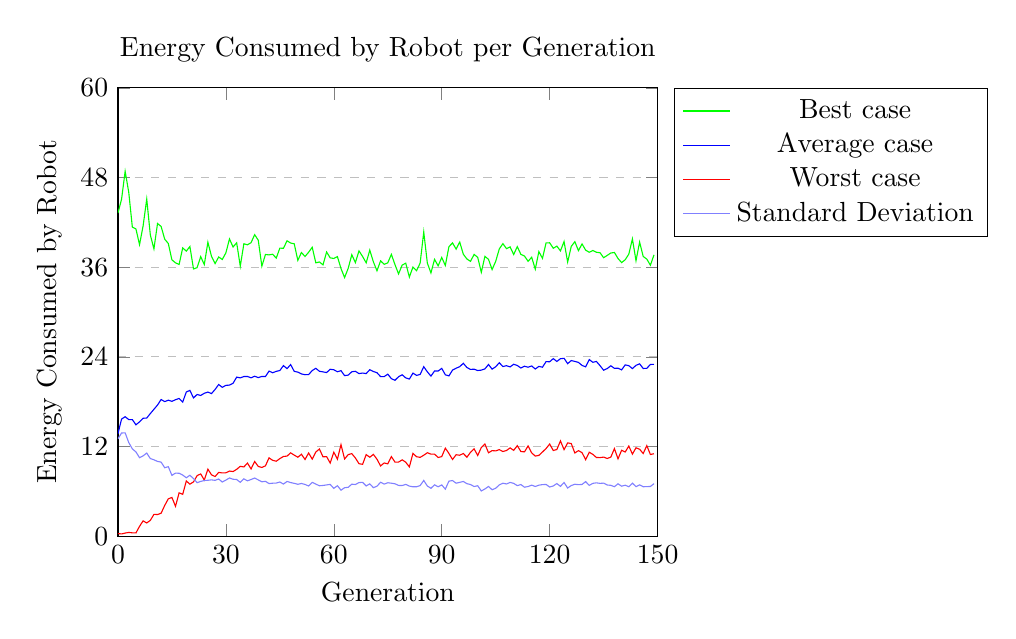
\begin{tikzpicture}
\begin{axis}[
	title={Energy Consumed by Robot per Generation},
	xlabel={Generation},
	ylabel={Energy Consumed by Robot},
	xmin=0, xmax=150,
	ymin=0, ymax=60,
	xtick={0.0,30.0,60.0,90.0,120.0,150.0},
	ytick={0.0,12.0,24.0,36.0,48.0,60.0},
	legend pos=outer north east,
	ymajorgrids=true,
	grid style=dashed,
]

\addplot[
	color=green,
	]
	coordinates {
	(0,43.25)(1,45.083333333333336)(2,48.83333333333335)(3,46.03333333333334)(4,41.36666666666666)(5,41.11666666666667)(6,39.016666666666666)(7,41.550000000000004)(8,45.11666666666667)(9,40.31666666666667)(10,38.45)(11,41.85)(12,41.45)(13,39.75)(14,39.166666666666664)(15,36.98333333333333)(16,36.58333333333333)(17,36.36666666666666)(18,38.583333333333336)(19,38.15)(20,38.76666666666666)(21,35.76666666666667)(22,35.93333333333334)(23,37.41666666666667)(24,36.349999999999994)(25,39.349999999999994)(26,37.45)(27,36.48333333333333)(28,37.36666666666667)(29,37.03333333333334)(30,37.916666666666664)(31,39.78333333333334)(32,38.7)(33,39.266666666666666)(34,36.13333333333334)(35,39.133333333333326)(36,39.0)(37,39.28333333333334)(38,40.35)(39,39.616666666666674)(40,36.13333333333333)(41,37.699999999999996)(42,37.65)(43,37.73333333333333)(44,37.21666666666666)(45,38.550000000000004)(46,38.533333333333324)(47,39.53333333333333)(48,39.23333333333334)(49,39.13333333333333)(50,36.91666666666666)(51,37.96666666666666)(52,37.43333333333333)(53,38.00000000000001)(54,38.666666666666664)(55,36.58333333333333)(56,36.7)(57,36.31666666666666)(58,38.03333333333334)(59,37.25)(60,37.166666666666664)(61,37.41666666666667)(62,35.81666666666667)(63,34.61666666666667)(64,35.85)(65,37.666666666666664)(66,36.61666666666666)(67,38.18333333333334)(68,37.43333333333334)(69,36.58333333333333)(70,38.283333333333324)(71,36.71666666666667)(72,35.516666666666666)(73,36.85)(74,36.383333333333326)(75,36.583333333333336)(76,37.71666666666666)(77,36.35)(78,35.099999999999994)(79,36.283333333333324)(80,36.53333333333333)(81,34.68333333333333)(82,36.016666666666666)(83,35.53333333333334)(84,36.55000000000001)(85,40.71666666666666)(86,36.550000000000004)(87,35.23333333333333)(88,37.05)(89,36.18333333333334)(90,37.300000000000004)(91,36.233333333333334)(92,38.74999999999999)(93,39.24999999999999)(94,38.416666666666664)(95,39.36666666666666)(96,37.73333333333333)(97,37.1)(98,36.783333333333324)(99,37.71666666666666)(100,37.316666666666656)(101,35.31666666666666)(102,37.45000000000001)(103,37.05)(104,35.68333333333334)(105,36.78333333333333)(106,38.45000000000001)(107,39.15)(108,38.48333333333334)(109,38.71666666666666)(110,37.7)(111,38.74999999999999)(112,37.716666666666676)(113,37.5)(114,36.78333333333334)(115,37.333333333333336)(116,35.73333333333334)(117,38.083333333333336)(118,37.18333333333333)(119,39.25)(120,39.266666666666666)(121,38.533333333333346)(122,38.81666666666666)(123,38.18333333333334)(124,39.43333333333334)(125,36.68333333333334)(126,38.78333333333333)(127,39.41666666666667)(128,38.21666666666666)(129,39.11666666666667)(130,38.283333333333346)(131,38.00000000000001)(132,38.233333333333334)(133,37.99999999999999)(134,37.93333333333334)(135,37.266666666666666)(136,37.58333333333333)(137,37.9)(138,37.96666666666666)(139,37.16666666666667)(140,36.61666666666667)(141,37.0)(142,37.74999999999999)(143,39.78333333333334)(144,36.86666666666667)(145,39.36666666666667)(146,37.43333333333332)(147,37.08333333333332)(148,36.266666666666666)(149,37.65)
	};
	\addlegendentry{Best case}
\addplot[
	color=blue,
	]
	coordinates {
	(0,13.702777777777778)(1,15.670833333333333)(2,15.987500000000002)(3,15.606944444444443)(4,15.60625)(5,14.904861111111112)(6,15.30625)(7,15.784722222222225)(8,15.807638888888889)(9,16.409722222222225)(10,16.98194444444444)(11,17.552083333333336)(12,18.293055555555554)(13,18.010416666666664)(14,18.200000000000006)(15,18.050694444444446)(16,18.263888888888886)(17,18.436805555555555)(18,17.95486111111111)(19,19.290277777777778)(20,19.51875)(21,18.50138888888889)(22,18.96666666666667)(23,18.831944444444442)(24,19.120833333333334)(25,19.286805555555556)(26,19.08402777777778)(27,19.638194444444444)(28,20.29722222222222)(29,19.926388888888887)(30,20.186805555555555)(31,20.217361111111103)(32,20.465277777777775)(33,21.289583333333336)(34,21.18402777777778)(35,21.365277777777777)(36,21.377083333333335)(37,21.192361111111104)(38,21.40902777777778)(39,21.22291666666667)(40,21.378472222222225)(41,21.37013888888889)(42,22.09791666666667)(43,21.87152777777778)(44,22.058333333333326)(45,22.175000000000004)(46,22.830555555555552)(47,22.42430555555556)(48,22.962500000000006)(49,22.059722222222224)(50,21.957638888888887)(51,21.714583333333334)(52,21.6125)(53,21.627083333333335)(54,22.167361111111113)(55,22.463888888888885)(56,22.072222222222223)(57,21.988194444444442)(58,21.89930555555555)(59,22.336805555555554)(60,22.274305555555557)(61,22.006249999999998)(62,22.15763888888889)(63,21.486111111111114)(64,21.55902777777778)(65,22.004166666666666)(66,22.067361111111115)(67,21.762500000000003)(68,21.833333333333332)(69,21.759722222222226)(70,22.28194444444445)(71,22.036805555555553)(72,21.87569444444444)(73,21.354166666666664)(74,21.36319444444445)(75,21.684027777777775)(76,21.082638888888887)(77,20.862499999999994)(78,21.340972222222227)(79,21.60138888888888)(80,21.183333333333337)(81,21.02638888888889)(82,21.827083333333338)(83,21.518055555555563)(84,21.647916666666667)(85,22.684027777777782)(86,21.996527777777775)(87,21.42222222222222)(88,22.109027777777783)(89,22.104166666666664)(90,22.463888888888896)(91,21.59861111111111)(92,21.452083333333334)(93,22.227777777777774)(94,22.484722222222224)(95,22.687500000000004)(96,23.14027777777778)(97,22.568055555555556)(98,22.320138888888888)(99,22.35)(100,22.170138888888886)(101,22.223611111111108)(102,22.390972222222224)(103,22.979166666666664)(104,22.352083333333333)(105,22.680555555555557)(106,23.212500000000006)(107,22.70486111111111)(108,22.821527777777778)(109,22.656944444444445)(110,23.00902777777778)(111,22.84861111111111)(112,22.50347222222222)(113,22.745138888888892)(114,22.614583333333332)(115,22.784027777777776)(116,22.374305555555555)(117,22.72222222222222)(118,22.616666666666667)(119,23.363194444444442)(120,23.34236111111111)(121,23.764583333333334)(122,23.384027777777774)(123,23.75555555555556)(124,23.80277777777778)(125,23.087499999999995)(126,23.505555555555556)(127,23.390277777777776)(128,23.258333333333333)(129,22.853472222222223)(130,22.66388888888889)(131,23.641666666666666)(132,23.27361111111111)(133,23.385416666666668)(134,22.819444444444446)(135,22.214583333333337)(136,22.436111111111114)(137,22.80347222222222)(138,22.46527777777777)(139,22.475694444444446)(140,22.26111111111111)(141,22.92777777777778)(142,22.820138888888895)(143,22.431250000000002)(144,22.865277777777777)(145,23.065277777777776)(146,22.44444444444444)(147,22.46944444444445)(148,22.98333333333333)(149,22.987500000000004)
	};
	\addlegendentry{Average case}
\addplot[
	color=red,
	]
	coordinates {
	(0,0.35)(1,0.3)(2,0.41666666666666663)(3,0.49999999999999994)(4,0.44999999999999996)(5,0.4333333333333333)(6,1.3166666666666667)(7,2.0500000000000003)(8,1.7666666666666668)(9,2.1166666666666667)(10,2.9166666666666665)(11,2.9)(12,3.066666666666667)(13,4.116666666666667)(14,5.0)(15,5.183333333333333)(16,4.0)(17,5.8)(18,5.6)(19,7.383333333333332)(20,6.966666666666667)(21,7.266666666666666)(22,8.100000000000001)(23,8.333333333333332)(24,7.516666666666666)(25,8.966666666666669)(26,8.216666666666667)(27,7.983333333333333)(28,8.533333333333333)(29,8.466666666666667)(30,8.483333333333334)(31,8.716666666666667)(32,8.649999999999999)(33,8.950000000000001)(34,9.349999999999998)(35,9.266666666666666)(36,9.783333333333333)(37,9.0)(38,10.0)(39,9.333333333333334)(40,9.2)(41,9.416666666666668)(42,10.483333333333334)(43,10.150000000000002)(44,10.033333333333331)(45,10.38333333333333)(46,10.666666666666668)(47,10.716666666666665)(48,11.149999999999999)(49,10.850000000000001)(50,10.566666666666668)(51,10.966666666666665)(52,10.266666666666666)(53,11.133333333333335)(54,10.316666666666665)(55,11.266666666666667)(56,11.666666666666666)(57,10.616666666666665)(58,10.65)(59,9.783333333333335)(60,11.250000000000002)(61,10.3)(62,12.25)(63,10.333333333333334)(64,10.916666666666664)(65,11.05)(66,10.466666666666669)(67,9.7)(68,9.616666666666667)(69,10.916666666666666)(70,10.566666666666666)(71,10.95)(72,10.300000000000002)(73,9.399999999999999)(74,9.8)(75,9.683333333333332)(76,10.65)(77,9.916666666666666)(78,9.916666666666668)(79,10.216666666666665)(80,9.9)(81,9.266666666666666)(82,11.083333333333334)(83,10.633333333333335)(84,10.549999999999997)(85,10.833333333333334)(86,11.166666666666668)(87,10.983333333333334)(88,10.983333333333333)(89,10.533333333333335)(90,10.65)(91,11.783333333333333)(92,11.066666666666666)(93,10.266666666666667)(94,10.9)(95,10.833333333333332)(96,11.066666666666665)(97,10.566666666666665)(98,11.233333333333333)(99,11.683333333333334)(100,10.8)(101,11.866666666666667)(102,12.333333333333332)(103,11.166666666666663)(104,11.450000000000001)(105,11.416666666666666)(106,11.583333333333334)(107,11.333333333333332)(108,11.466666666666669)(109,11.816666666666666)(110,11.483333333333334)(111,12.116666666666669)(112,11.333333333333334)(113,11.283333333333335)(114,12.083333333333334)(115,11.150000000000002)(116,10.716666666666667)(117,10.816666666666668)(118,11.266666666666667)(119,11.733333333333333)(120,12.333333333333334)(121,11.46666666666667)(122,11.6)(123,12.75)(124,11.583333333333332)(125,12.483333333333333)(126,12.4)(127,11.133333333333331)(128,11.45)(129,11.183333333333332)(130,10.233333333333334)(131,11.233333333333334)(132,10.95)(133,10.533333333333331)(134,10.516666666666667)(135,10.583333333333334)(136,10.399999999999999)(137,10.583333333333332)(138,11.716666666666667)(139,10.35)(140,11.5)(141,11.266666666666664)(142,12.066666666666668)(143,10.983333333333334)(144,11.833333333333334)(145,11.633333333333335)(146,11.066666666666665)(147,12.116666666666669)(148,10.933333333333332)(149,11.033333333333335)
	};
	\addlegendentry{Worst case}
\addplot[
	color=blue!50,
	]
	coordinates {
	(0,13.025428908389014)(1,13.810346550954476)(2,13.828080440847092)(3,12.536856175323127)(4,11.687336506557788)(5,11.278266565587925)(6,10.501986791555993)(7,10.756807752498277)(8,11.123641785695767)(9,10.386590504187978)(10,10.221378626796373)(11,10.0072642842455)(12,9.910259443748078)(13,9.159101324569477)(14,9.303068720464928)(15,8.136114284424643)(16,8.442985588951556)(17,8.419964631951537)(18,8.175106742249568)(19,7.819965516568136)(20,8.152075255391479)(21,7.7114696165346075)(22,7.163779102298379)(23,7.328275304469596)(24,7.4528129284425715)(25,7.481462069336689)(26,7.53842600557016)(27,7.473568842213835)(28,7.652880221410522)(29,7.24745306007676)(30,7.507851449040219)(31,7.789290167969191)(32,7.622416740108644)(33,7.579573710866637)(34,7.209173054431467)(35,7.674179762512963)(36,7.404567722923065)(37,7.587610754448604)(38,7.777959745378355)(39,7.534920928418523)(40,7.276515574031566)(41,7.342139720134329)(42,7.041825948290563)(43,7.090418939649814)(44,7.110711609579553)(45,7.249430618270159)(46,6.97307712015094)(47,7.326380735304754)(48,7.175603845053802)(49,7.071456064751343)(50,6.944892436659276)(51,7.054153593681907)(52,6.925574599185686)(53,6.71816819439981)(54,7.2027313196276594)(55,6.969585256429113)(56,6.747240707808752)(57,6.789921258148179)(58,6.860547540788126)(59,6.928211569219866)(60,6.397805765611721)(61,6.7552421370725675)(62,6.154926673906596)(63,6.485800688397053)(64,6.541500249927993)(65,6.9578287440314055)(66,6.916514655024321)(67,7.171383562116569)(68,7.208015117309649)(69,6.719545525884519)(70,7.0064607939101995)(71,6.492097867347669)(72,6.682439569654588)(73,7.222453389940815)(74,6.969889252912186)(75,7.15245677645985)(76,7.0899056889959375)(77,7.014635159627206)(78,6.791903957601484)(79,6.780344653994618)(80,6.931501668919507)(81,6.7026144154052005)(82,6.6093845948443715)(83,6.6114720266694675)(84,6.776284790786758)(85,7.458544733301797)(86,6.715603927290007)(87,6.40997058389649)(88,6.875571233475309)(89,6.607686022952553)(90,6.861778369888345)(91,6.296488869387335)(92,7.369711299557141)(93,7.444854372659652)(94,7.089891736321568)(95,7.2078004568368925)(96,7.320265729199365)(97,7.027339192380647)(98,6.912254402661862)(99,6.649402026643729)(100,6.748778337282881)(101,6.047367568958867)(102,6.323465498320564)(103,6.651838777617148)(104,6.211944896853704)(105,6.417052304513479)(106,6.860288720300009)(107,7.08864869544486)(108,6.987562242631174)(109,7.195008862591659)(110,7.067679970742447)(111,6.764544671818376)(112,6.910756018467242)(113,6.5563145115801875)(114,6.646507909579263)(115,6.832896938087492)(116,6.650187882020349)(117,6.825224031089765)(118,6.902161583494312)(119,6.925290955648311)(120,6.580437646884687)(121,6.718299856719031)(122,7.040225022091886)(123,6.66810757240103)(124,7.1883639796633565)(125,6.445244453108852)(126,6.7778886188033365)(127,6.948772922857561)(128,6.895431573334017)(129,6.9246965479096385)(130,7.303813108654388)(131,6.797754897530904)(132,7.0714504518847106)(133,7.141901757424131)(134,7.064649642995899)(135,7.101780349676218)(136,6.850000503981754)(137,6.8067826374503815)(138,6.6211205492311365)(139,7.014587725641828)(140,6.69178681032594)(141,6.8212860961759905)(142,6.6210763034866185)(143,7.093520058043778)(144,6.6268579715702)(145,6.870033969272324)(146,6.6170758597207495)(147,6.633982989863595)(148,6.652876244562766)(149,7.028843944036023)
	};
	\addlegendentry{Standard Deviation}
\end{axis}
\end{tikzpicture}
}
		\caption{Some sample caption}
		\label{fig:energy-consumed-by-robot-easy}
	\end{subfigure}%
	\begin{subfigure}[b]{0.7\textwidth}
		\centering
		\resizebox{0.9\linewidth}{!}{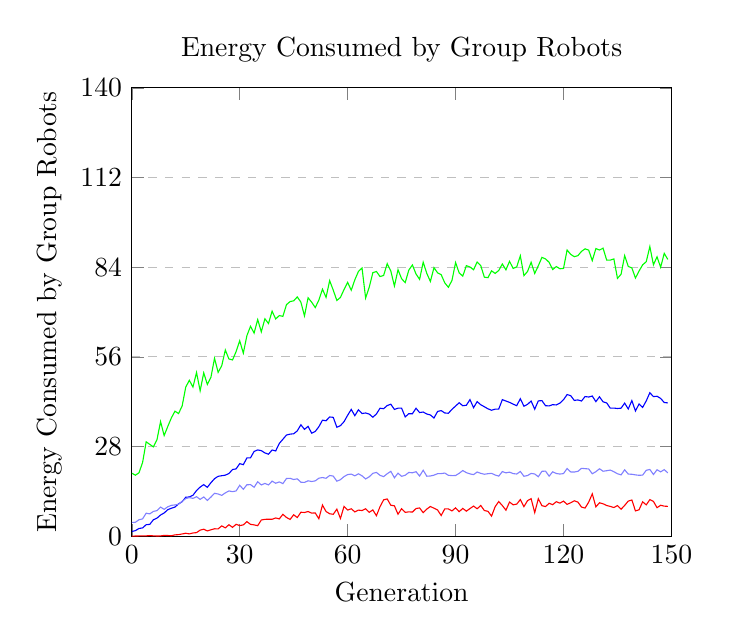
\begin{tikzpicture}
\begin{axis}[
	title={Energy Consumed by Group Robots},
	xlabel={Generation},
	ylabel={Energy Consumed by Group Robots},
	xmin=0, xmax=150,
	ymin=0, ymax=140,
	xtick={0.0,30.0,60.0,90.0,120.0,150.0},
	ytick={0.0,28.0,56.0,84.0,112.0,140.0},
	ymajorgrids=true,
	grid style=dashed,
]

\addplot[
	color=green,
	]
	coordinates {
	(0,19.68333333333333)(1,19.05)(2,19.800000000000004)(3,23.0)(4,29.46666666666666)(5,28.66666666666666)(6,27.900000000000006)(7,30.116666666666656)(8,35.78333333333334)(9,31.416666666666664)(10,34.266666666666666)(11,36.93333333333333)(12,39.03333333333334)(13,38.3)(14,40.666666666666664)(15,46.56666666666666)(16,48.68333333333334)(17,46.56666666666666)(18,51.116666666666674)(19,45.383333333333326)(20,50.99999999999999)(21,47.38333333333333)(22,49.616666666666674)(23,55.56666666666666)(24,51.16666666666666)(25,53.21666666666667)(26,58.15)(27,55.349999999999994)(28,55.03333333333333)(29,57.63333333333333)(30,61.01666666666666)(31,57.166666666666664)(32,62.63333333333335)(33,65.55)(34,63.43333333333332)(35,67.64999999999999)(36,63.81666666666668)(37,67.9)(38,66.41666666666667)(39,70.28333333333332)(40,67.83333333333331)(41,68.89999999999999)(42,68.65000000000002)(43,72.30000000000001)(44,73.26666666666668)(45,73.5)(46,74.71666666666665)(47,73.1)(48,68.8)(49,74.45)(50,73.08333333333334)(51,71.38333333333333)(52,73.73333333333333)(53,77.14999999999999)(54,74.56666666666665)(55,79.8)(56,76.83333333333333)(57,73.61666666666665)(58,74.56666666666669)(59,77.05000000000001)(60,79.24999999999999)(61,76.81666666666669)(62,80.06666666666666)(63,82.68333333333334)(64,83.75)(65,74.36666666666667)(66,77.73333333333333)(67,82.28333333333336)(68,82.64999999999999)(69,81.08333333333331)(70,81.41666666666666)(71,85.1)(72,82.81666666666668)(73,78.13333333333334)(74,83.19999999999999)(75,80.4)(76,79.18333333333335)(77,83.1)(78,84.69999999999999)(79,81.9)(80,80.19999999999999)(81,85.56666666666666)(82,82.06666666666668)(83,79.55000000000001)(84,83.86666666666666)(85,82.25)(86,81.66666666666666)(87,79.11666666666667)(88,77.73333333333332)(89,79.86666666666667)(90,85.46666666666667)(91,82.21666666666664)(92,81.21666666666665)(93,84.48333333333332)(94,84.06666666666668)(95,83.20000000000002)(96,85.63333333333334)(97,84.5)(98,80.88333333333333)(99,80.73333333333333)(100,82.86666666666669)(101,82.06666666666666)(102,82.96666666666667)(103,84.99999999999999)(104,83.18333333333335)(105,85.83333333333333)(106,83.60000000000001)(107,84.10000000000001)(108,87.56666666666666)(109,81.36666666666665)(110,82.66666666666666)(111,85.53333333333333)(112,82.05)(113,84.45)(114,87.06666666666666)(115,86.60000000000001)(116,85.53333333333332)(117,83.26666666666667)(118,84.20000000000002)(119,83.51666666666668)(120,83.61666666666669)(121,89.36666666666666)(122,88.01666666666668)(123,87.28333333333332)(124,87.60000000000002)(125,88.93333333333332)(126,89.73333333333335)(127,89.33333333333334)(128,86.04999999999998)(129,89.81666666666668)(130,89.36666666666667)(131,89.93333333333335)(132,86.23333333333333)(133,86.2)(134,86.58333333333333)(135,80.51666666666665)(136,81.78333333333332)(137,87.6)(138,84.23333333333333)(139,83.78333333333335)(140,80.61666666666666)(141,82.79999999999998)(142,84.73333333333335)(143,85.71666666666665)(144,90.45000000000002)(145,84.75)(146,87.25000000000001)(147,83.96666666666667)(148,88.31666666666668)(149,86.43333333333332)
	};
\addplot[
	color=blue,
	]
	coordinates {
	(0,1.4493055555555556)(1,1.7402777777777778)(2,2.4076388888888887)(3,2.5819444444444444)(4,3.5854166666666667)(5,3.692361111111111)(6,5.127083333333332)(7,5.63888888888889)(8,6.620833333333333)(9,7.252083333333332)(10,8.265277777777778)(11,8.738194444444446)(12,9.101388888888888)(13,10.08125)(14,10.765277777777778)(15,12.162500000000001)(16,12.256944444444445)(17,12.770138888888889)(18,14.259027777777774)(19,15.331944444444442)(20,16.100694444444443)(21,15.260416666666666)(22,16.70486111111111)(23,17.95277777777778)(24,18.69236111111111)(25,18.883333333333333)(26,19.063194444444438)(27,19.570833333333336)(28,20.820833333333333)(29,21.018749999999997)(30,22.664583333333333)(31,22.329166666666666)(32,24.445138888888888)(33,24.46944444444445)(34,26.471527777777776)(35,26.93125)(36,26.719444444444445)(37,26.008333333333336)(38,25.60138888888889)(39,26.923611111111104)(40,26.626388888888886)(41,28.961111111111112)(42,30.273611111111112)(43,31.591666666666665)(44,31.87291666666666)(45,31.984027777777783)(46,32.88680555555555)(47,34.790972222222216)(48,33.365972222222226)(49,34.29722222222222)(50,32.173611111111114)(51,32.70416666666667)(52,34.19375000000001)(53,36.235416666666666)(54,36.04999999999998)(55,37.226388888888884)(56,37.118055555555564)(57,34.013888888888886)(58,34.52291666666666)(59,35.77222222222222)(60,37.755555555555546)(61,39.6)(62,37.637499999999996)(63,39.48680555555555)(64,38.30902777777777)(65,38.47777777777779)(66,38.13472222222222)(67,37.14652777777777)(68,38.172916666666666)(69,39.96319444444444)(70,39.813194444444456)(71,40.79583333333333)(72,41.215277777777764)(73,39.584722222222226)(74,39.97083333333333)(75,39.97291666666667)(76,37.25277777777777)(77,38.25694444444444)(78,38.22916666666667)(79,39.95069444444446)(80,38.60902777777778)(81,38.77500000000001)(82,38.153472222222234)(83,37.86805555555555)(84,36.900000000000006)(85,38.956944444444446)(86,39.21875000000001)(87,38.48125)(88,38.39236111111112)(89,39.615277777777784)(90,40.64166666666667)(91,41.67569444444444)(92,40.74166666666667)(93,40.892361111111114)(94,42.648611111111116)(95,40.12430555555556)(96,42.02708333333332)(97,41.047222222222224)(98,40.42430555555555)(99,39.772916666666674)(100,39.331250000000004)(101,39.672222222222224)(102,39.71041666666666)(103,42.641666666666666)(104,42.20625)(105,41.793749999999996)(106,41.233333333333334)(107,40.75902777777778)(108,42.93958333333333)(109,40.58958333333332)(110,41.170833333333334)(111,42.202083333333334)(112,39.6625)(113,42.25486111111111)(114,42.334722222222226)(115,40.75000000000001)(116,40.68750000000001)(117,41.072222222222216)(118,40.97986111111111)(119,41.560416666666676)(120,42.61736111111111)(121,44.22569444444444)(122,43.88333333333333)(123,42.394444444444446)(124,42.55694444444443)(125,42.211111111111116)(126,43.6076388888889)(127,43.4625)(128,43.76666666666666)(129,42.02361111111111)(130,43.53611111111112)(131,41.96041666666667)(132,41.624305555555544)(133,39.97430555555556)(134,40.00555555555555)(135,39.87569444444444)(136,39.97708333333334)(137,41.54930555555555)(138,39.72638888888888)(139,42.34652777777777)(140,39.09097222222223)(141,41.294444444444444)(142,40.22361111111111)(143,42.24513888888889)(144,44.80277777777777)(145,43.58333333333333)(146,43.69930555555556)(147,43.02430555555556)(148,41.73888888888888)(149,41.625)
	};
\addplot[
	color=red,
	]
	coordinates {
	(0,0.016666666666666666)(1,0.05)(2,0.08333333333333333)(3,0.08333333333333333)(4,0.09999999999999999)(5,0.19999999999999998)(6,0.09999999999999999)(7,0.06666666666666667)(8,0.08333333333333334)(9,0.25)(10,0.21666666666666667)(11,0.13333333333333333)(12,0.41666666666666663)(13,0.4833333333333333)(14,0.7)(15,0.9166666666666666)(16,0.7166666666666667)(17,1.0000000000000002)(18,1.1166666666666667)(19,1.9000000000000001)(20,2.183333333333333)(21,1.6499999999999997)(22,2.0)(23,2.316666666666667)(24,2.283333333333333)(25,3.2166666666666663)(26,2.6)(27,3.5833333333333335)(28,2.7666666666666666)(29,3.7166666666666663)(30,3.3000000000000003)(31,3.5333333333333337)(32,4.55)(33,3.6999999999999993)(34,3.5333333333333328)(35,3.2833333333333328)(36,5.05)(37,5.266666666666667)(38,5.299999999999999)(39,5.283333333333333)(40,5.699999999999999)(41,5.4)(42,6.833333333333334)(43,5.85)(44,5.233333333333333)(45,6.683333333333334)(46,5.816666666666667)(47,7.4833333333333325)(48,7.400000000000002)(49,7.699999999999999)(50,7.216666666666667)(51,7.250000000000001)(52,5.449999999999998)(53,9.733333333333333)(54,7.7)(55,7.0166666666666675)(56,6.833333333333332)(57,8.450000000000001)(58,5.533333333333332)(59,9.316666666666665)(60,8.149999999999999)(61,8.566666666666668)(62,7.6)(63,8.149999999999999)(64,8.0)(65,8.583333333333332)(66,7.449999999999999)(67,8.2)(68,6.3999999999999995)(69,9.216666666666665)(70,11.35)(71,11.633333333333333)(72,9.666666666666666)(73,9.483333333333334)(74,6.866666666666666)(75,8.6)(76,7.450000000000001)(77,7.600000000000001)(78,7.533333333333333)(79,8.633333333333335)(80,8.816666666666668)(81,7.35)(82,8.466666666666665)(83,9.283333333333335)(84,8.733333333333333)(85,8.183333333333334)(86,6.466666666666667)(87,8.549999999999999)(88,8.516666666666666)(89,7.9)(90,8.850000000000001)(91,7.649999999999999)(92,8.683333333333334)(93,7.8166666666666655)(94,8.633333333333336)(95,9.4)(96,8.566666666666668)(97,9.583333333333334)(98,8.016666666666667)(99,7.766666666666666)(100,6.266666666666666)(101,9.216666666666665)(102,10.816666666666668)(103,9.566666666666665)(104,8.116666666666667)(105,10.666666666666668)(106,9.799999999999999)(107,10.016666666666666)(108,11.433333333333334)(109,9.233333333333333)(110,11.1)(111,11.716666666666669)(112,7.366666666666666)(113,11.7)(114,9.533333333333333)(115,9.250000000000002)(116,10.266666666666666)(117,9.85)(118,10.766666666666666)(119,10.333333333333334)(120,10.950000000000001)(121,9.95)(122,10.433333333333334)(123,11.05)(124,10.65)(125,9.1)(126,8.783333333333335)(127,10.633333333333335)(128,13.216666666666669)(129,9.166666666666664)(130,10.433333333333334)(131,10.116666666666667)(132,9.583333333333332)(133,9.299999999999999)(134,8.95)(135,9.566666666666666)(136,8.416666666666668)(137,9.616666666666667)(138,10.966666666666665)(139,11.3)(140,7.8999999999999995)(141,8.25)(142,10.733333333333333)(143,9.783333333333333)(144,11.416666666666666)(145,10.85)(146,8.899999999999999)(147,9.666666666666668)(148,9.383333333333335)(149,9.316666666666668)
	};
\addplot[
	color=blue!50,
	]
	coordinates {
	(0,4.28643110259652)(1,4.350004465706617)(2,5.1353585814671305)(3,5.4036342055382836)(4,7.184036432091683)(5,6.959859072520352)(6,7.740183076680505)(7,7.9895584403415265)(8,9.095487652655299)(9,8.382295176141476)(10,9.175423944208907)(11,9.633879288381019)(12,9.768514050354678)(13,9.974388115867566)(14,10.894458482255986)(15,11.738536762885685)(16,12.052917874791023)(17,11.809426929647783)(18,12.327754549882282)(19,11.491843569692882)(20,12.24759609905034)(21,11.17672592269558)(22,12.219402932220374)(23,13.39188482037835)(24,13.177696287681739)(25,12.74766297624472)(26,13.521821381657194)(27,14.135044010423613)(28,13.906055403578163)(29,14.128742493983314)(30,15.902322644410466)(31,14.645396418128552)(32,16.060336930196915)(33,16.099668682455683)(34,15.28406147186754)(35,16.99790090836383)(36,15.996187485351106)(37,16.48239954714082)(38,16.016387608916656)(39,17.18999929190662)(40,16.538603152238476)(41,16.947777823923516)(42,16.424612841552417)(43,18.01001504802194)(44,18.078239704517717)(45,17.704079890445904)(46,17.913934301523216)(47,16.852624241279187)(48,16.790068127011928)(49,17.295830669086403)(50,17.078290689305945)(51,17.275993085175653)(52,18.117950075812907)(53,18.311959715112405)(54,18.08517279742271)(55,18.953098229289978)(56,18.767837639776488)(57,17.172012659257902)(58,17.65097508376289)(59,18.62404914701312)(60,19.238944827068806)(61,19.392432617191513)(62,18.845586300539566)(63,19.48640298916557)(64,18.858058411573936)(65,17.878337930467147)(66,18.55605846283305)(67,19.63556833827702)(68,19.915277309552184)(69,19.006921915917616)(70,18.597254446813317)(71,19.509070380318636)(72,20.262762845648705)(73,18.2368857544476)(74,19.674839801461772)(75,18.69521328303294)(76,19.030233509955085)(77,19.907718252012586)(78,19.79814700277209)(79,20.137561765560616)(80,18.795355068425618)(81,20.59535530390388)(82,18.72987040604221)(83,18.798325829024964)(84,19.060857959296605)(85,19.51787743213442)(86,19.54489190339996)(87,19.711786355157944)(88,19.009380833146565)(89,18.927774516737333)(90,18.947015282128955)(91,19.638613342366703)(92,20.49930164229917)(93,19.853511291764768)(94,19.459606929036465)(95,19.23188996151202)(96,20.038325925091844)(97,19.61997688067101)(98,19.3507354587123)(99,19.514163896455432)(100,19.631598058091992)(101,19.109664015582222)(102,18.756192501638573)(103,20.180840343035893)(104,19.773228850286245)(105,20.002454347760107)(106,19.54912126207232)(107,19.418074851634312)(108,20.206758169014982)(109,18.710740906744913)(110,18.93617145351968)(111,19.61620260966329)(112,19.423176715801702)(113,18.560247256359798)(114,20.25783868884567)(115,20.325005765811206)(116,18.75070538397598)(117,20.099168440707494)(118,19.587735379855705)(119,19.40600950617213)(120,19.551509454546206)(121,21.13214833612396)(122,20.06398796601037)(123,20.037555187318954)(124,20.250837917539858)(125,21.193432242675417)(126,21.09177383269476)(127,20.992179395339345)(128,19.496413740982774)(129,20.14352512409504)(130,21.052582318385543)(131,20.286633139465597)(132,20.450394077134284)(133,20.64914510944557)(134,20.137723555109858)(135,19.499307880893333)(136,19.146987961702894)(137,20.7307583172003)(138,19.39964134770471)(139,19.335344872430053)(140,19.146794263155318)(141,19.01098423522314)(142,19.07965716709215)(143,20.57695874353471)(144,20.839029859801943)(145,19.26633036046936)(146,20.748815778140724)(147,20.091755087016924)(148,20.79314639778314)(149,19.767443043138652)
	};
\end{axis}
\end{tikzpicture}
}
		\caption{Some sample caption}
		\label{fig:energy-consumed-by-group-easy}
	\end{subfigure}%

}
\caption{Figure shows results from a simulation in the easy environment (p.2)}
\end{figure}





\newpage





\subsubsection{Difficult Environment}

\newpage

\vspace*{-2.0cm}
\textbf{\Huge Results - Hard environment (1) }
\vspace{1.5cm}
\begin{tikzpicture}[remember picture,overlay]
   \node[anchor=south east,inner sep=20pt] at (current page.south east)
              {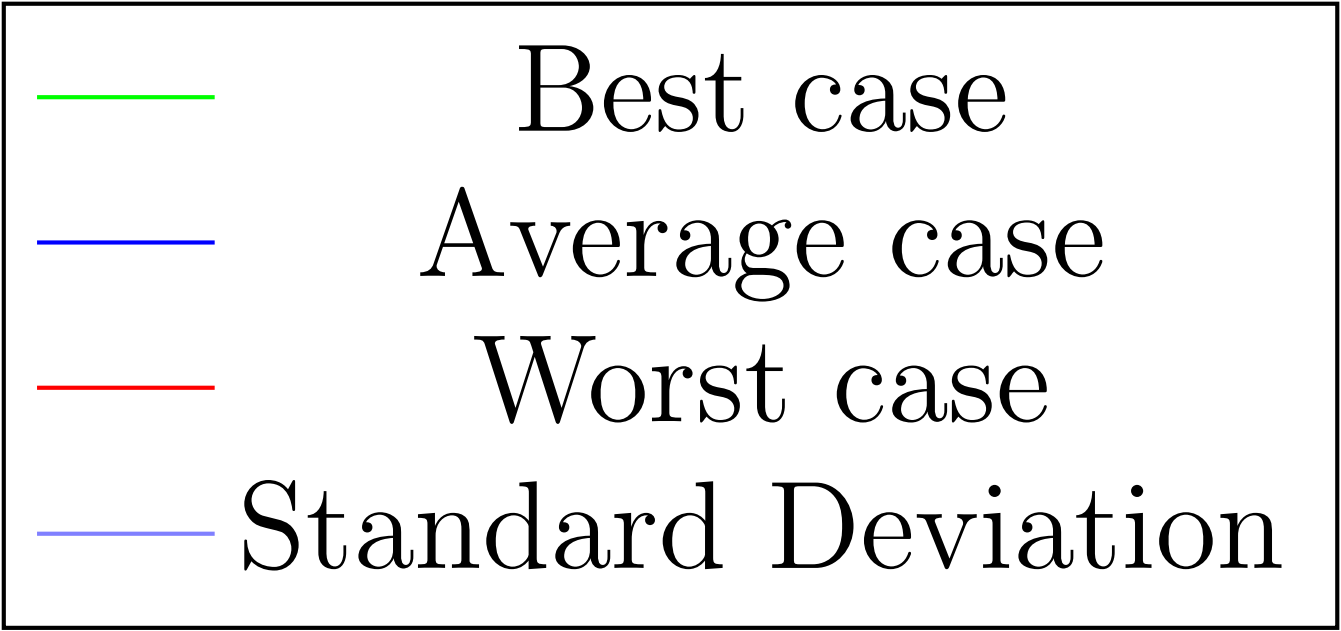
\includegraphics[scale=0.1]{chapters/res/generated_graph_legend.png}};
\end{tikzpicture}

\begin{figure}[H]
\vspace*{-1cm}
	\makebox[\linewidth][c]{%
	\begin{subfigure}[b]{0.7\textwidth}
		\centering
		\resizebox{0.9\linewidth}{!}{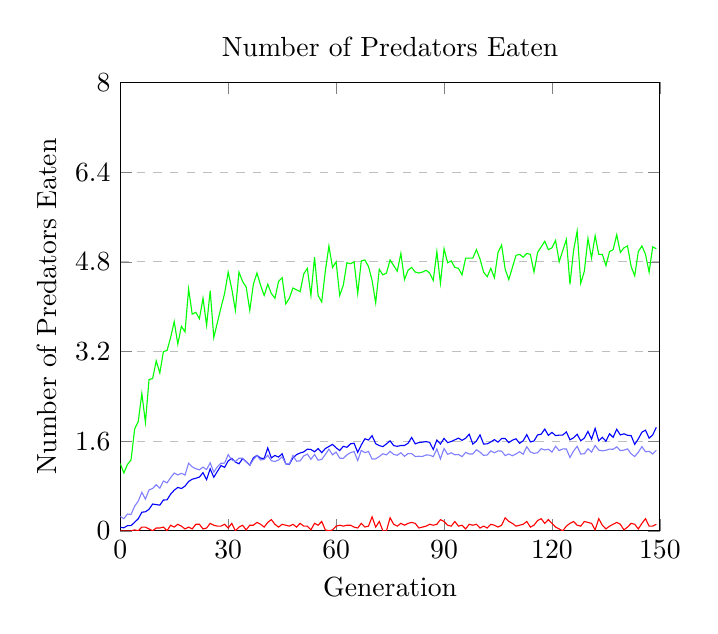
\begin{tikzpicture}
\begin{axis}[
	title={Number of Predators Eaten},
	xlabel={Generation},
	ylabel={Number of Predators Eaten},
	xmin=0, xmax=150,
	ymin=0, ymax=8,
	xtick={0.0,30.0,60.0,90.0,120.0,150.0},
	ytick={0.0,1.6,3.2,4.800000000000001,6.4,8.0},
	ymajorgrids=true,
	grid style=dashed,
]

\addplot[
	color=green,
	]
	coordinates {
	(0,1.2)(1,1.0333333333333334)(2,1.1833333333333333)(3,1.2666666666666668)(4,1.8166666666666664)(5,1.95)(6,2.45)(7,1.9333333333333333)(8,2.7)(9,2.7166666666666663)(10,3.033333333333334)(11,2.8166666666666664)(12,3.1999999999999997)(13,3.2166666666666663)(14,3.45)(15,3.7333333333333334)(16,3.3333333333333335)(17,3.6500000000000004)(18,3.55)(19,4.316666666666666)(20,3.8666666666666663)(21,3.9000000000000004)(22,3.7833333333333337)(23,4.1499999999999995)(24,3.6666666666666665)(25,4.283333333333333)(26,3.45)(27,3.716666666666667)(28,3.9833333333333334)(29,4.2333333333333325)(30,4.616666666666666)(31,4.316666666666666)(32,3.9333333333333336)(33,4.616666666666667)(34,4.450000000000001)(35,4.35)(36,3.9333333333333336)(37,4.4)(38,4.6)(39,4.383333333333334)(40,4.2)(41,4.4)(42,4.2333333333333325)(43,4.1499999999999995)(44,4.449999999999999)(45,4.516666666666667)(46,4.05)(47,4.15)(48,4.333333333333335)(49,4.3)(50,4.2666666666666675)(51,4.583333333333334)(52,4.683333333333334)(53,4.2)(54,4.883333333333334)(55,4.200000000000001)(56,4.083333333333333)(57,4.633333333333333)(58,5.083333333333333)(59,4.699999999999999)(60,4.800000000000001)(61,4.2)(62,4.383333333333334)(63,4.783333333333332)(64,4.766666666666667)(65,4.799999999999999)(66,4.233333333333333)(67,4.8166666666666655)(68,4.833333333333333)(69,4.716666666666667)(70,4.466666666666667)(71,4.066666666666667)(72,4.666666666666666)(73,4.5666666666666655)(74,4.6)(75,4.833333333333333)(76,4.733333333333333)(77,4.633333333333333)(78,4.949999999999999)(79,4.483333333333333)(80,4.6499999999999995)(81,4.7)(82,4.616666666666667)(83,4.599999999999999)(84,4.616666666666666)(85,4.6499999999999995)(86,4.6)(87,4.466666666666668)(88,4.9833333333333325)(89,4.416666666666667)(90,5.033333333333333)(91,4.783333333333333)(92,4.8166666666666655)(93,4.699999999999998)(94,4.683333333333334)(95,4.566666666666666)(96,4.866666666666665)(97,4.866666666666667)(98,4.866666666666665)(99,5.016666666666666)(100,4.8500000000000005)(101,4.616666666666666)(102,4.533333333333332)(103,4.683333333333334)(104,4.516666666666667)(105,4.966666666666667)(106,5.1)(107,4.666666666666666)(108,4.483333333333333)(109,4.699999999999999)(110,4.916666666666668)(111,4.933333333333334)(112,4.883333333333334)(113,4.95)(114,4.9333333333333345)(115,4.616666666666666)(116,4.966666666666667)(117,5.066666666666666)(118,5.166666666666666)(119,5.016666666666667)(120,5.05)(121,5.183333333333334)(122,4.8)(123,4.999999999999999)(124,5.2)(125,4.4)(126,4.999999999999998)(127,5.35)(128,4.416666666666667)(129,4.633333333333333)(130,5.216666666666667)(131,4.866666666666667)(132,5.266666666666666)(133,4.933333333333334)(134,4.933333333333334)(135,4.733333333333333)(136,4.983333333333333)(137,5.016666666666667)(138,5.283333333333332)(139,4.966666666666666)(140,5.050000000000001)(141,5.083333333333332)(142,4.716666666666666)(143,4.550000000000001)(144,4.9833333333333325)(145,5.083333333333333)(146,4.933333333333333)(147,4.616666666666666)(148,5.066666666666666)(149,5.033333333333333)
	};
\addplot[
	color=blue,
	]
	coordinates {
	(0,0.0625)(1,0.05416666666666667)(2,0.09236111111111112)(3,0.09236111111111113)(4,0.15347222222222218)(5,0.2145833333333333)(6,0.33124999999999993)(7,0.34027777777777773)(8,0.38402777777777775)(9,0.47847222222222213)(10,0.467361111111111)(11,0.45833333333333326)(12,0.5499999999999998)(13,0.5520833333333334)(14,0.6541666666666668)(15,0.7249999999999999)(16,0.7743055555555558)(17,0.7548611111111111)(18,0.7972222222222223)(19,0.8805555555555554)(20,0.9208333333333333)(21,0.9375)(22,0.9590277777777778)(23,1.0375000000000003)(24,0.9124999999999999)(25,1.1055555555555554)(26,0.9555555555555554)(27,1.0604166666666666)(28,1.1638888888888888)(29,1.1326388888888888)(30,1.246527777777778)(31,1.29375)(32,1.2284722222222226)(33,1.195833333333333)(34,1.2875)(35,1.2368055555555557)(36,1.1701388888888893)(37,1.3020833333333333)(38,1.3465277777777778)(39,1.2979166666666668)(40,1.2881944444444446)(41,1.4784722222222226)(42,1.3006944444444444)(43,1.3451388888888889)(44,1.315277777777778)(45,1.3749999999999998)(46,1.1944444444444444)(47,1.1868055555555557)(48,1.3020833333333333)(49,1.3583333333333334)(50,1.3895833333333334)(51,1.407638888888889)(52,1.4576388888888887)(53,1.4513888888888888)(54,1.4097222222222223)(55,1.467361111111111)(56,1.3944444444444444)(57,1.4680555555555557)(58,1.5048611111111112)(59,1.542361111111111)(60,1.4819444444444443)(61,1.4326388888888892)(62,1.5083333333333333)(63,1.4902777777777783)(64,1.5527777777777776)(65,1.5618055555555557)(66,1.4)(67,1.5333333333333337)(68,1.6423611111111112)(69,1.6194444444444447)(70,1.697916666666667)(71,1.5541666666666667)(72,1.5208333333333335)(73,1.502083333333333)(74,1.551388888888889)(75,1.605555555555556)(76,1.5201388888888894)(77,1.507638888888889)(78,1.5222222222222224)(79,1.5222222222222224)(80,1.5624999999999998)(81,1.6666666666666663)(82,1.5520833333333333)(83,1.5743055555555556)(84,1.582638888888889)(85,1.5916666666666668)(86,1.5784722222222223)(87,1.4513888888888888)(88,1.619444444444445)(89,1.5499999999999996)(90,1.649305555555556)(91,1.5736111111111108)(92,1.5937500000000002)(93,1.623611111111111)(94,1.6541666666666666)(95,1.614583333333333)(96,1.6513888888888886)(97,1.7243055555555555)(98,1.5479166666666664)(99,1.6020833333333333)(100,1.7118055555555556)(101,1.5479166666666666)(102,1.5527777777777778)(103,1.5854166666666667)(104,1.6270833333333334)(105,1.5819444444444444)(106,1.6465277777777776)(107,1.6479166666666667)(108,1.5736111111111108)(109,1.6173611111111117)(110,1.6423611111111112)(111,1.5618055555555557)(112,1.607638888888889)(113,1.717361111111111)(114,1.5861111111111112)(115,1.6027777777777779)(116,1.7111111111111115)(117,1.724305555555555)(118,1.815277777777778)(119,1.7027777777777777)(120,1.7569444444444444)(121,1.7)(122,1.7069444444444444)(123,1.7090277777777778)(124,1.7652777777777775)(125,1.6243055555555554)(126,1.6597222222222223)(127,1.722222222222222)(128,1.60625)(129,1.6555555555555554)(130,1.7736111111111108)(131,1.6361111111111106)(132,1.8277777777777775)(133,1.6048611111111113)(134,1.6680555555555554)(135,1.5993055555555555)(136,1.73125)(137,1.6680555555555556)(138,1.8118055555555554)(139,1.7104166666666667)(140,1.7312500000000002)(141,1.7041666666666668)(142,1.6993055555555556)(143,1.543055555555555)(144,1.6402777777777777)(145,1.7597222222222222)(146,1.7958333333333334)(147,1.6541666666666666)(148,1.7097222222222224)(149,1.8465277777777775)
	};
\addplot[
	color=red,
	]
	coordinates {
	(0,0.0)(1,0.0)(2,0.0)(3,0.0)(4,0.016666666666666666)(5,0.0)(6,0.06666666666666667)(7,0.06666666666666667)(8,0.03333333333333333)(9,0.0)(10,0.05)(11,0.05)(12,0.06666666666666667)(13,0.0)(14,0.1)(15,0.06666666666666667)(16,0.11666666666666667)(17,0.08333333333333334)(18,0.03333333333333333)(19,0.06666666666666667)(20,0.03333333333333333)(21,0.11666666666666667)(22,0.11666666666666667)(23,0.03333333333333333)(24,0.05)(25,0.13333333333333333)(26,0.1)(27,0.08333333333333334)(28,0.08333333333333334)(29,0.11666666666666667)(30,0.05)(31,0.13333333333333333)(32,0.0)(33,0.06666666666666667)(34,0.1)(35,0.016666666666666666)(36,0.1)(37,0.1)(38,0.15)(39,0.11666666666666665)(40,0.06666666666666667)(41,0.15)(42,0.19999999999999998)(43,0.11666666666666667)(44,0.06666666666666667)(45,0.11666666666666667)(46,0.1)(47,0.08333333333333333)(48,0.11666666666666667)(49,0.06666666666666667)(50,0.13333333333333333)(51,0.08333333333333334)(52,0.08333333333333333)(53,0.016666666666666666)(54,0.13333333333333333)(55,0.1)(56,0.16666666666666666)(57,0.016666666666666666)(58,0.0)(59,0.016666666666666666)(60,0.08333333333333333)(61,0.1)(62,0.08333333333333333)(63,0.1)(64,0.1)(65,0.06666666666666667)(66,0.05)(67,0.13333333333333333)(68,0.06666666666666667)(69,0.08333333333333334)(70,0.24999999999999997)(71,0.06666666666666667)(72,0.16666666666666666)(73,0.0)(74,0.0)(75,0.2333333333333333)(76,0.11666666666666667)(77,0.08333333333333334)(78,0.13333333333333333)(79,0.09999999999999999)(80,0.13333333333333333)(81,0.15)(82,0.13333333333333333)(83,0.05)(84,0.06666666666666667)(85,0.08333333333333334)(86,0.11666666666666667)(87,0.1)(88,0.11666666666666667)(89,0.19999999999999998)(90,0.16666666666666666)(91,0.1)(92,0.08333333333333334)(93,0.16666666666666666)(94,0.08333333333333333)(95,0.1)(96,0.03333333333333333)(97,0.11666666666666667)(98,0.1)(99,0.11666666666666667)(100,0.05)(101,0.08333333333333334)(102,0.05)(103,0.11666666666666667)(104,0.09999999999999999)(105,0.06666666666666667)(106,0.1)(107,0.2333333333333333)(108,0.16666666666666666)(109,0.13333333333333333)(110,0.08333333333333333)(111,0.09999999999999999)(112,0.11666666666666667)(113,0.16666666666666666)(114,0.06666666666666667)(115,0.1)(116,0.18333333333333332)(117,0.21666666666666665)(118,0.13333333333333333)(119,0.19999999999999998)(120,0.13333333333333333)(121,0.06666666666666667)(122,0.03333333333333333)(123,0.0)(124,0.08333333333333333)(125,0.13333333333333333)(126,0.16666666666666666)(127,0.1)(128,0.08333333333333333)(129,0.16666666666666666)(130,0.15)(131,0.13333333333333333)(132,0.016666666666666666)(133,0.21666666666666665)(134,0.1)(135,0.03333333333333333)(136,0.08333333333333334)(137,0.11666666666666667)(138,0.15)(139,0.11666666666666667)(140,0.016666666666666666)(141,0.06666666666666667)(142,0.13333333333333333)(143,0.11666666666666667)(144,0.03333333333333333)(145,0.13333333333333333)(146,0.21666666666666665)(147,0.08333333333333334)(148,0.08333333333333333)(149,0.11666666666666667)
	};
\addplot[
	color=blue!50,
	]
	coordinates {
	(0,0.2567954586689933)(1,0.21629302775326373)(2,0.29920191485009023)(3,0.2917842860052699)(4,0.43938342611972053)(5,0.5298369903444883)(6,0.6873650424798703)(7,0.5659532033530428)(8,0.7297232936301211)(9,0.7562454027031459)(10,0.8224362592002558)(11,0.7604420089605098)(12,0.8884160818389348)(13,0.8558256675827959)(14,0.949200206948469)(15,1.0317455747521904)(16,0.9967686637648429)(17,1.0252715523862075)(18,0.9954271054797319)(19,1.206136175477242)(20,1.1415173509733176)(21,1.1079419833568562)(22,1.0880919702263587)(23,1.137001155109919)(24,1.0943035855783534)(25,1.2133976947676983)(26,1.045167325264568)(27,1.1444597482179737)(28,1.2057437200887111)(29,1.207006085856858)(30,1.3596970133505712)(31,1.2663909971018068)(32,1.2376025607000565)(33,1.2949883630135817)(34,1.2954343724501953)(35,1.2288708410924596)(36,1.1686294658132759)(37,1.2706605872502297)(38,1.3414481240707854)(39,1.264150269180343)(40,1.2742046493352315)(41,1.3490831072151277)(42,1.2500501865067586)(43,1.2375737939119473)(44,1.2633880233226185)(45,1.3202650000204446)(46,1.197479554826585)(47,1.1903955467406375)(48,1.3440609264808963)(49,1.2424043325695717)(50,1.2481356533589825)(51,1.3367010999474396)(52,1.3690356952150462)(53,1.275743932705493)(54,1.3614850755144656)(55,1.2600310621842614)(56,1.2745093554985076)(57,1.361182498474822)(58,1.4569455141031105)(59,1.356445306887592)(60,1.4046999807623346)(61,1.2959300380622536)(62,1.293074279873345)(63,1.354286951624945)(64,1.3952056236588637)(65,1.4150506451628497)(66,1.2529736101027726)(67,1.4357940836252543)(68,1.3944339029414623)(69,1.4159059009838726)(70,1.2789197138192603)(71,1.2840493739316572)(72,1.3261680493358272)(73,1.3753443259570692)(74,1.3550459424269616)(75,1.4187104766158183)(76,1.363266470358261)(77,1.3483264132399708)(78,1.3934828964094277)(79,1.329994211296116)(80,1.378364512826987)(81,1.377828735532433)(82,1.3260238723402658)(83,1.3304993318180296)(84,1.3267253015240073)(85,1.3535989021598125)(86,1.35025706436527)(87,1.3235071445105966)(88,1.4604813466608608)(89,1.28127439821142)(90,1.470162284717902)(91,1.364341394001647)(92,1.392461287390359)(93,1.3565811952094564)(94,1.3614993997368516)(95,1.3241004828149456)(96,1.3996515364229842)(97,1.3710041273057996)(98,1.371718036039779)(99,1.4468404464847928)(100,1.4046186835167647)(101,1.346464299416398)(102,1.3531902904051816)(103,1.4272891255473228)(104,1.3915631833793658)(105,1.4265844183796499)(106,1.4226527573203374)(107,1.342168301343959)(108,1.3701282904084517)(109,1.3384810713146797)(110,1.3720313722187614)(111,1.4111536257843982)(112,1.3668462715075946)(113,1.5007794996073955)(114,1.4070458745893863)(115,1.3808119367266334)(116,1.394442224909498)(117,1.4650073572029583)(118,1.443160942058554)(119,1.4565992214116765)(120,1.4055073672201828)(121,1.5082402418775767)(122,1.4319743496640134)(123,1.4613611003038145)(124,1.4601469545553467)(125,1.3076995324109888)(126,1.4237984753090769)(127,1.5078658177238164)(128,1.368939341391302)(129,1.3758217751105597)(130,1.4647220952274642)(131,1.4038274578024166)(132,1.5235658440892983)(133,1.4399870181163297)(134,1.4272968610701615)(135,1.4374197605233643)(136,1.4581450173104689)(137,1.4543316025882906)(138,1.499030213581117)(139,1.4313398215750164)(140,1.4394016109833991)(141,1.4619107340953532)(142,1.3740528031658596)(143,1.3255783287870362)(144,1.402239531501261)(145,1.503277663037369)(146,1.4095204305005509)(147,1.4190285375644207)(148,1.3704329774235906)(149,1.43738691981063)
	};
\end{axis}
\end{tikzpicture}
}
		\caption{Some sample caption}
	\end{subfigure}%
	\begin{subfigure}[b]{0.7\textwidth}	
		\centering
		\resizebox{0.9\linewidth}{!}{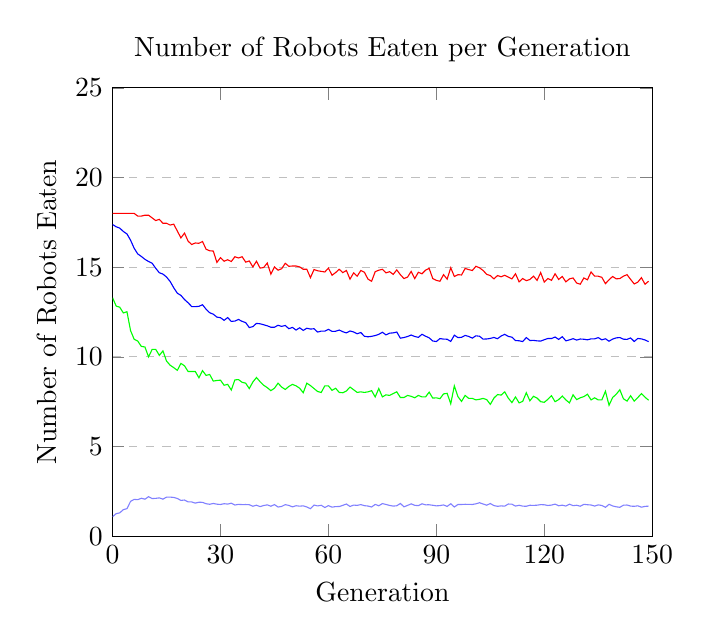
\begin{tikzpicture}
\begin{axis}[
	title={Number of Robots Eaten per Generation},
	xlabel={Generation},
	ylabel={Number of Robots Eaten},
	xmin=0, xmax=150,
	ymin=0, ymax=25,
	xtick={0.0,30.0,60.0,90.0,120.0,150.0},
	ytick={0.0,5.0,10.0,15.0,20.0,25.0},
	ymajorgrids=true,
	grid style=dashed,
]

\addplot[
	color=red,
	]
	coordinates {
	(0,18.0)(1,18.0)(2,18.0)(3,18.0)(4,18.0)(5,18.0)(6,18.0)(7,17.85)(8,17.85)(9,17.9)(10,17.9)(11,17.750000000000004)(12,17.6)(13,17.666666666666668)(14,17.45)(15,17.45)(16,17.35)(17,17.4)(18,17.01666666666667)(19,16.633333333333336)(20,16.900000000000002)(21,16.450000000000003)(22,16.26666666666667)(23,16.35)(24,16.333333333333332)(25,16.433333333333337)(26,16.000000000000004)(27,15.91666666666667)(28,15.9)(29,15.266666666666666)(30,15.533333333333333)(31,15.333333333333332)(32,15.416666666666666)(33,15.316666666666666)(34,15.583333333333332)(35,15.516666666666667)(36,15.583333333333334)(37,15.283333333333335)(38,15.349999999999998)(39,15.016666666666666)(40,15.333333333333336)(41,14.949999999999998)(42,14.983333333333333)(43,15.233333333333334)(44,14.616666666666665)(45,15.016666666666666)(46,14.833333333333336)(47,14.916666666666666)(48,15.216666666666667)(49,15.049999999999999)(50,15.066666666666668)(51,15.066666666666665)(52,15.016666666666667)(53,14.883333333333333)(54,14.883333333333335)(55,14.416666666666666)(56,14.866666666666667)(57,14.8)(58,14.766666666666666)(59,14.733333333333334)(60,14.950000000000001)(61,14.549999999999997)(62,14.700000000000003)(63,14.883333333333335)(64,14.7)(65,14.81666666666667)(66,14.333333333333334)(67,14.683333333333335)(68,14.500000000000002)(69,14.816666666666666)(70,14.716666666666667)(71,14.33333333333333)(72,14.216666666666667)(73,14.749999999999998)(74,14.833333333333336)(75,14.883333333333336)(76,14.683333333333334)(77,14.750000000000004)(78,14.6)(79,14.85)(80,14.583333333333336)(81,14.366666666666665)(82,14.45)(83,14.766666666666666)(84,14.366666666666665)(85,14.716666666666665)(86,14.633333333333335)(87,14.833333333333332)(88,14.933333333333335)(89,14.366666666666667)(90,14.266666666666664)(91,14.216666666666667)(92,14.583333333333336)(93,14.333333333333332)(94,14.966666666666669)(95,14.48333333333333)(96,14.583333333333334)(97,14.566666666666666)(98,14.933333333333334)(99,14.866666666666665)(100,14.816666666666666)(101,15.05)(102,14.966666666666667)(103,14.816666666666666)(104,14.600000000000001)(105,14.533333333333333)(106,14.350000000000001)(107,14.533333333333333)(108,14.466666666666665)(109,14.55)(110,14.450000000000003)(111,14.35)(112,14.633333333333333)(113,14.183333333333335)(114,14.366666666666665)(115,14.249999999999998)(116,14.316666666666666)(117,14.499999999999996)(118,14.266666666666666)(119,14.700000000000001)(120,14.166666666666664)(121,14.366666666666667)(122,14.266666666666667)(123,14.633333333333333)(124,14.316666666666668)(125,14.483333333333333)(126,14.183333333333335)(127,14.349999999999998)(128,14.4)(129,14.116666666666669)(130,14.049999999999995)(131,14.400000000000004)(132,14.3)(133,14.733333333333336)(134,14.5)(135,14.5)(136,14.433333333333335)(137,14.083333333333334)(138,14.3)(139,14.48333333333333)(140,14.350000000000001)(141,14.366666666666665)(142,14.5)(143,14.583333333333332)(144,14.316666666666668)(145,14.066666666666663)(146,14.166666666666664)(147,14.416666666666668)(148,14.049999999999997)(149,14.216666666666667)
	};
\addplot[
	color=blue,
	]
	coordinates {
	(0,17.38125)(1,17.25486111111111)(2,17.179166666666664)(3,16.991666666666667)(4,16.856944444444444)(5,16.506944444444443)(6,16.056250000000002)(7,15.74027777777778)(8,15.6)(9,15.439583333333335)(10,15.318749999999998)(11,15.221527777777782)(12,14.937500000000002)(13,14.691666666666666)(14,14.615972222222222)(15,14.452083333333334)(16,14.206944444444442)(17,13.854861111111113)(18,13.549999999999999)(19,13.428472222222224)(20,13.195833333333331)(21,13.01527777777778)(22,12.805555555555554)(23,12.800000000000002)(24,12.81875)(25,12.905555555555555)(26,12.656944444444445)(27,12.461111111111112)(28,12.378472222222223)(29,12.216666666666669)(30,12.183333333333337)(31,12.037499999999998)(32,12.190972222222223)(33,11.977777777777778)(34,11.996527777777779)(35,12.08611111111111)(36,11.981249999999998)(37,11.910416666666666)(38,11.634027777777774)(39,11.686805555555553)(40,11.868750000000002)(41,11.844444444444445)(42,11.790277777777776)(43,11.731944444444443)(44,11.652777777777779)(45,11.654166666666669)(46,11.760416666666668)(47,11.699305555555554)(48,11.751388888888888)(49,11.570833333333335)(50,11.643055555555556)(51,11.495833333333332)(52,11.62013888888889)(53,11.477083333333335)(54,11.597222222222221)(55,11.549305555555554)(56,11.569444444444443)(57,11.38125)(58,11.436805555555555)(59,11.431944444444447)(60,11.533333333333337)(61,11.42222222222222)(62,11.426388888888889)(63,11.496527777777777)(64,11.401388888888889)(65,11.3375)(66,11.443750000000001)(67,11.388194444444444)(68,11.288194444444443)(69,11.357638888888886)(70,11.14861111111111)(71,11.118055555555555)(72,11.145138888888889)(73,11.188194444444447)(74,11.256944444444445)(75,11.372916666666667)(76,11.227083333333333)(77,11.32291666666667)(78,11.3375)(79,11.384722222222221)(80,11.042361111111111)(81,11.07777777777778)(82,11.135416666666668)(83,11.218055555555557)(84,11.135416666666668)(85,11.088194444444444)(86,11.258333333333331)(87,11.153472222222224)(88,11.061805555555559)(89,10.885416666666664)(90,10.85486111111111)(91,11.019444444444447)(92,10.990972222222222)(93,10.983333333333334)(94,10.859722222222222)(95,11.207638888888887)(96,11.072916666666668)(97,11.090277777777775)(98,11.195833333333331)(99,11.139583333333334)(100,11.044444444444446)(101,11.174305555555557)(102,11.149305555555557)(103,10.990277777777779)(104,10.997222222222222)(105,11.02986111111111)(106,11.082638888888889)(107,11.012500000000001)(108,11.163194444444445)(109,11.255555555555556)(110,11.141666666666666)(111,11.09861111111111)(112,10.91111111111111)(113,10.897222222222219)(114,10.853472222222223)(115,11.075694444444446)(116,10.9125)(117,10.919444444444444)(118,10.891666666666667)(119,10.879861111111111)(120,10.956944444444444)(121,11.025000000000002)(122,11.022222222222222)(123,11.106250000000001)(124,10.975000000000001)(125,11.125694444444443)(126,10.89236111111111)(127,10.94861111111111)(128,11.015277777777778)(129,10.935416666666669)(130,10.995138888888889)(131,10.982638888888888)(132,10.951388888888888)(133,11.004166666666668)(134,11.00486111111111)(135,11.072916666666666)(136,10.95)(137,11.008333333333335)(138,10.872916666666667)(139,10.99236111111111)(140,11.059722222222225)(141,11.077083333333334)(142,10.986111111111107)(143,10.975)(144,11.056249999999999)(145,10.858333333333333)(146,11.026388888888887)(147,11.002083333333333)(148,10.941666666666663)(149,10.849999999999998)
	};
\addplot[
	color=green,
	]
	coordinates {
	(0,13.299999999999999)(1,12.833333333333334)(2,12.766666666666667)(3,12.450000000000001)(4,12.516666666666667)(5,11.466666666666665)(6,10.983333333333333)(7,10.883333333333335)(8,10.583333333333334)(9,10.55)(10,10.0)(11,10.416666666666668)(12,10.416666666666666)(13,10.083333333333334)(14,10.333333333333332)(15,9.766666666666666)(16,9.533333333333335)(17,9.4)(18,9.249999999999998)(19,9.633333333333335)(20,9.500000000000002)(21,9.183333333333332)(22,9.183333333333335)(23,9.183333333333334)(24,8.833333333333332)(25,9.233333333333334)(26,8.966666666666667)(27,9.016666666666667)(28,8.650000000000002)(29,8.683333333333334)(30,8.7)(31,8.416666666666668)(32,8.466666666666669)(33,8.15)(34,8.716666666666669)(35,8.733333333333333)(36,8.583333333333334)(37,8.533333333333333)(38,8.233333333333334)(39,8.600000000000001)(40,8.85)(41,8.616666666666667)(42,8.416666666666666)(43,8.283333333333335)(44,8.116666666666667)(45,8.250000000000002)(46,8.533333333333335)(47,8.316666666666666)(48,8.183333333333334)(49,8.350000000000001)(50,8.466666666666667)(51,8.383333333333333)(52,8.250000000000002)(53,8.0)(54,8.533333333333333)(55,8.400000000000002)(56,8.233333333333334)(57,8.066666666666666)(58,8.016666666666667)(59,8.383333333333335)(60,8.383333333333335)(61,8.133333333333333)(62,8.250000000000002)(63,8.016666666666666)(64,7.999999999999999)(65,8.1)(66,8.316666666666666)(67,8.166666666666668)(68,8.016666666666667)(69,8.05)(70,8.016666666666667)(71,8.05)(72,8.116666666666667)(73,7.766666666666668)(74,8.233333333333334)(75,7.766666666666666)(76,7.8833333333333355)(77,7.850000000000002)(78,7.95)(79,8.05)(80,7.733333333333335)(81,7.733333333333333)(82,7.850000000000002)(83,7.799999999999998)(84,7.716666666666669)(85,7.850000000000001)(86,7.7666666666666675)(87,7.766666666666667)(88,8.033333333333333)(89,7.699999999999999)(90,7.716666666666667)(91,7.666666666666668)(92,7.933333333333333)(93,7.966666666666669)(94,7.3833333333333355)(95,8.383333333333333)(96,7.783333333333332)(97,7.516666666666667)(98,7.8500000000000005)(99,7.683333333333332)(100,7.683333333333334)(101,7.6)(102,7.633333333333335)(103,7.683333333333335)(104,7.616666666666667)(105,7.3500000000000005)(106,7.699999999999999)(107,7.900000000000001)(108,7.866666666666667)(109,8.05)(110,7.700000000000002)(111,7.449999999999998)(112,7.7666666666666675)(113,7.433333333333334)(114,7.5166666666666675)(115,8.000000000000002)(116,7.550000000000001)(117,7.800000000000002)(118,7.699999999999998)(119,7.500000000000001)(120,7.466666666666667)(121,7.633333333333334)(122,7.833333333333335)(123,7.5)(124,7.616666666666667)(125,7.816666666666668)(126,7.600000000000001)(127,7.433333333333335)(128,7.883333333333335)(129,7.616666666666669)(130,7.716666666666667)(131,7.783333333333333)(132,7.916666666666668)(133,7.600000000000001)(134,7.716666666666668)(135,7.6000000000000005)(136,7.6)(137,8.083333333333336)(138,7.3)(139,7.733333333333334)(140,7.916666666666666)(141,8.166666666666668)(142,7.666666666666665)(143,7.533333333333331)(144,7.833333333333335)(145,7.533333333333334)(146,7.733333333333333)(147,7.949999999999999)(148,7.75)(149,7.583333333333333)
	};
\addplot[
	color=blue!50,
	]
	coordinates {
	(0,1.0845553930560614)(1,1.2569338975860094)(2,1.3017983326147198)(3,1.4808281183298073)(4,1.5368804893331904)(5,1.9414565911936879)(6,2.052438579185581)(7,2.0371261762853474)(8,2.1147316306649677)(9,2.0644475504300304)(10,2.2027891777900086)(11,2.0974227426931784)(12,2.1099997400216015)(13,2.1365971943227424)(14,2.0647111376362184)(15,2.179269219016812)(16,2.1789261262717727)(17,2.162328782803921)(18,2.103319594799526)(19,1.9964660276363264)(20,2.0169980862615615)(21,1.913533661859874)(22,1.9103853828804676)(23,1.845100614466328)(24,1.894540488688379)(25,1.8879539015113127)(26,1.810227541690253)(27,1.7796893021754037)(28,1.8263200645558042)(29,1.7852800826213544)(30,1.7691009754808276)(31,1.811943203641366)(32,1.7894988814919188)(33,1.8413266258642207)(34,1.7394693229722307)(35,1.773349402933656)(36,1.7626908875390925)(37,1.7650052221532893)(38,1.755056004005871)(39,1.6694770087006683)(40,1.7288978782220779)(41,1.6490058014997229)(42,1.7108563175169367)(43,1.7469725300722967)(44,1.672308898221016)(45,1.76198673162835)(46,1.6269161630694104)(47,1.6604690006506309)(48,1.7601992732088814)(49,1.7157687549258058)(50,1.6355864658257606)(51,1.698269369571266)(52,1.6745451327979028)(53,1.6925176675911218)(54,1.6281014739767259)(55,1.5343649292329151)(56,1.73725373034437)(57,1.687577789854123)(58,1.7239662513624021)(59,1.6012136998670252)(60,1.7033664792675265)(61,1.6190976867359137)(62,1.6522349123607005)(63,1.653489949972742)(64,1.7204828953420213)(65,1.7947295405532513)(66,1.657043752441505)(67,1.734310023298112)(68,1.7185881263641383)(69,1.7624345107154464)(70,1.7026454936666648)(71,1.680907611237149)(72,1.6283055633317973)(73,1.7731331248221651)(74,1.6961798680916977)(75,1.8194971275218461)(76,1.7705839796084886)(77,1.7149739141094633)(78,1.6787291489883853)(79,1.6967526155660022)(80,1.8263891833335264)(81,1.6360192742802997)(82,1.7170426061537163)(83,1.8036798139515082)(84,1.7196475813775935)(85,1.7054149328387864)(86,1.8057918093378942)(87,1.7498508057083495)(88,1.7513803095709037)(89,1.7244946059843673)(90,1.6910670844633653)(91,1.7061525198522098)(92,1.743773515582125)(93,1.6601675697537441)(94,1.8085626729988915)(95,1.6268270636065576)(96,1.768183265427153)(97,1.7680085311295117)(98,1.7789371524196773)(99,1.7749789380496006)(100,1.7686108900810018)(101,1.805258918689446)(102,1.8662796521010188)(103,1.7930151082124868)(104,1.7283498944904854)(105,1.8222028549189824)(106,1.7064253771117204)(107,1.6664239861862777)(108,1.6902588219290244)(109,1.6754660062012563)(110,1.793923798977226)(111,1.7851497722087277)(112,1.6784761343327914)(113,1.724181263660402)(114,1.6753377493600876)(115,1.6688694545073928)(116,1.7249232675298631)(117,1.7170341456605627)(118,1.729609585662609)(119,1.7598630286745318)(120,1.752173949633828)(121,1.7130797373799131)(122,1.734320922850237)(123,1.7894755728712155)(124,1.6974486819961991)(125,1.7308083656229294)(126,1.6814474617269677)(127,1.7876011258282214)(128,1.702369609831248)(129,1.7243512522623894)(130,1.67156201349268)(131,1.7759576866332487)(132,1.7543351440765447)(133,1.7394384821476907)(134,1.6784968639697497)(135,1.7468641555926465)(136,1.711345018847415)(137,1.6089217547982122)(138,1.7777003360526693)(139,1.687782262115383)(140,1.6389884908846712)(141,1.6105802017887851)(142,1.72834116299074)(143,1.7380203270924734)(144,1.6792547265312)(145,1.6648842371869519)(146,1.6942252906511823)(147,1.6172386476929739)(148,1.6625562179078772)(149,1.675906672645179)
	};
\end{axis}
\end{tikzpicture}
}
		\caption{Some sample caption}
	\end{subfigure}%
}
\\
\\
\\
	\makebox[\linewidth][c]{%
	\begin{subfigure}[b]{0.7\textwidth}
		\centering
		\resizebox{0.9\linewidth}{!}{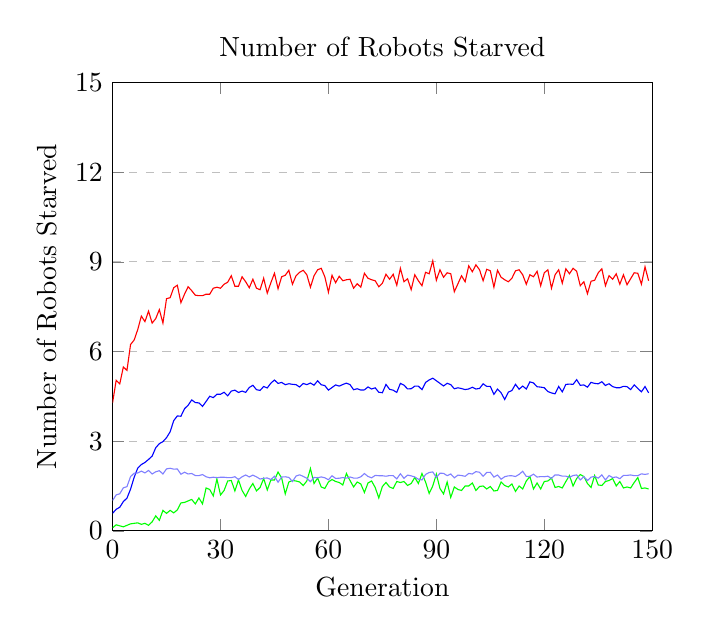
\begin{tikzpicture}
\begin{axis}[
	title={Number of Robots Starved},
	xlabel={Generation},
	ylabel={Number of Robots Starved},
	xmin=0, xmax=150,
	ymin=0, ymax=15,
	xtick={0.0,30.0,60.0,90.0,120.0,150.0},
	ytick={0.0,3.0,6.0,9.0,12.0,15.0},
	ymajorgrids=true,
	grid style=dashed,
]

\addplot[
	color=red,
	]
	coordinates {
	(0,4.283333333333333)(1,5.033333333333333)(2,4.916666666666666)(3,5.483333333333333)(4,5.366666666666665)(5,6.233333333333333)(6,6.383333333333333)(7,6.7333333333333325)(8,7.183333333333333)(9,7.0)(10,7.35)(11,6.949999999999999)(12,7.1)(13,7.400000000000001)(14,6.95)(15,7.766666666666667)(16,7.800000000000001)(17,8.133333333333333)(18,8.216666666666667)(19,7.633333333333334)(20,7.916666666666669)(21,8.166666666666668)(22,8.033333333333335)(23,7.883333333333335)(24,7.866666666666667)(25,7.866666666666667)(26,7.916666666666667)(27,7.916666666666667)(28,8.116666666666667)(29,8.15)(30,8.116666666666667)(31,8.25)(32,8.316666666666668)(33,8.533333333333333)(34,8.183333333333335)(35,8.183333333333334)(36,8.500000000000002)(37,8.333333333333334)(38,8.133333333333335)(39,8.416666666666668)(40,8.116666666666667)(41,8.066666666666666)(42,8.45)(43,7.95)(44,8.3)(45,8.616666666666667)(46,8.1)(47,8.500000000000002)(48,8.55)(49,8.716666666666667)(50,8.25)(51,8.533333333333335)(52,8.650000000000002)(53,8.716666666666667)(54,8.566666666666666)(55,8.15)(56,8.533333333333333)(57,8.733333333333334)(58,8.783333333333333)(59,8.500000000000004)(60,7.983333333333333)(61,8.55)(62,8.3)(63,8.516666666666667)(64,8.366666666666667)(65,8.400000000000002)(66,8.416666666666666)(67,8.116666666666667)(68,8.266666666666667)(69,8.150000000000002)(70,8.616666666666667)(71,8.450000000000001)(72,8.399999999999999)(73,8.366666666666669)(74,8.166666666666668)(75,8.283333333333333)(76,8.583333333333334)(77,8.416666666666668)(78,8.583333333333334)(79,8.216666666666665)(80,8.783333333333335)(81,8.333333333333332)(82,8.433333333333334)(83,8.066666666666666)(84,8.566666666666666)(85,8.366666666666665)(86,8.2)(87,8.65)(88,8.6)(89,9.033333333333333)(90,8.383333333333333)(91,8.733333333333333)(92,8.483333333333333)(93,8.633333333333333)(94,8.600000000000001)(95,8.000000000000002)(96,8.266666666666666)(97,8.533333333333331)(98,8.333333333333334)(99,8.866666666666665)(100,8.666666666666666)(101,8.900000000000002)(102,8.733333333333334)(103,8.366666666666667)(104,8.750000000000002)(105,8.700000000000001)(106,8.150000000000002)(107,8.716666666666667)(108,8.483333333333334)(109,8.399999999999999)(110,8.333333333333332)(111,8.450000000000001)(112,8.700000000000001)(113,8.733333333333333)(114,8.56666666666667)(115,8.25)(116,8.566666666666668)(117,8.500000000000002)(118,8.683333333333335)(119,8.2)(120,8.633333333333333)(121,8.733333333333334)(122,8.116666666666667)(123,8.566666666666668)(124,8.733333333333334)(125,8.283333333333333)(126,8.766666666666667)(127,8.6)(128,8.783333333333333)(129,8.683333333333332)(130,8.2)(131,8.333333333333332)(132,7.933333333333335)(133,8.35)(134,8.383333333333335)(135,8.633333333333333)(136,8.76666666666667)(137,8.2)(138,8.533333333333335)(139,8.416666666666668)(140,8.599999999999998)(141,8.249999999999998)(142,8.566666666666668)(143,8.23333333333333)(144,8.433333333333334)(145,8.633333333333335)(146,8.616666666666667)(147,8.249999999999998)(148,8.833333333333334)(149,8.366666666666667)
	};
\addplot[
	color=blue,
	]
	coordinates {
	(0,0.5847222222222224)(1,0.7194444444444447)(2,0.7881944444444445)(3,0.9784722222222224)(4,1.09375)(5,1.392361111111111)(6,1.789583333333333)(7,2.0993055555555555)(8,2.2166666666666663)(9,2.2868055555555555)(10,2.3881944444444443)(11,2.4993055555555554)(12,2.778472222222222)(13,2.916666666666667)(14,2.983333333333334)(15,3.116666666666666)(16,3.3118055555555563)(17,3.6868055555555554)(18,3.843055555555557)(19,3.8333333333333335)(20,4.085416666666665)(21,4.202083333333333)(22,4.379166666666667)(23,4.290972222222222)(24,4.279861111111113)(25,4.1618055555555555)(26,4.328472222222223)(27,4.502083333333332)(28,4.456250000000001)(29,4.569444444444444)(30,4.568055555555556)(31,4.636111111111111)(32,4.516666666666667)(33,4.674305555555556)(34,4.706944444444443)(35,4.628472222222223)(36,4.675694444444445)(37,4.631944444444445)(38,4.795138888888889)(39,4.8687499999999995)(40,4.7222222222222205)(41,4.697222222222222)(42,4.828472222222222)(43,4.779166666666666)(44,4.940277777777777)(45,5.045138888888889)(46,4.9319444444444445)(47,4.965277777777778)(48,4.888888888888888)(49,4.9208333333333325)(50,4.9006944444444445)(51,4.8909722222222225)(52,4.811111111111111)(53,4.929166666666665)(54,4.890277777777778)(55,4.94513888888889)(56,4.872222222222222)(57,5.020833333333332)(58,4.886805555555555)(59,4.8590277777777775)(60,4.708333333333333)(61,4.79375)(62,4.88263888888889)(63,4.840972222222222)(64,4.895138888888889)(65,4.940972222222222)(66,4.892361111111112)(67,4.720138888888888)(68,4.753472222222223)(69,4.709027777777778)(70,4.713888888888889)(71,4.813888888888889)(72,4.74375)(73,4.784722222222221)(74,4.636111111111112)(75,4.6201388888888895)(76,4.897916666666666)(77,4.7340277777777775)(78,4.704861111111111)(79,4.6305555555555555)(80,4.9326388888888895)(81,4.873611111111113)(82,4.747916666666667)(83,4.754166666666666)(84,4.8388888888888895)(85,4.839583333333334)(86,4.7236111111111105)(87,4.9638888888888895)(88,5.047222222222222)(89,5.1069444444444425)(90,5.021527777777777)(91,4.933333333333334)(92,4.845138888888889)(93,4.935416666666665)(94,4.8909722222222225)(95,4.752083333333333)(96,4.785416666666666)(97,4.759027777777777)(98,4.725)(99,4.746527777777778)(100,4.802777777777778)(101,4.745138888888889)(102,4.762500000000001)(103,4.919444444444443)(104,4.831944444444444)(105,4.832638888888889)(106,4.565277777777778)(107,4.742361111111111)(108,4.617361111111111)(109,4.393055555555557)(110,4.638888888888889)(111,4.69513888888889)(112,4.902777777777778)(113,4.736805555555557)(114,4.842361111111111)(115,4.744444444444445)(116,4.984027777777777)(117,4.947222222222223)(118,4.820138888888889)(119,4.808333333333333)(120,4.786805555555555)(121,4.659027777777778)(122,4.613194444444445)(123,4.582638888888888)(124,4.831944444444445)(125,4.65)(126,4.897222222222222)(127,4.909722222222223)(128,4.898611111111111)(129,5.0569444444444445)(130,4.8687499999999995)(131,4.8805555555555555)(132,4.8062499999999995)(133,4.967361111111111)(134,4.931250000000001)(135,4.918055555555555)(136,4.9875)(137,4.861805555555556)(138,4.920833333333333)(139,4.825694444444445)(140,4.788194444444444)(141,4.7868055555555555)(142,4.834027777777778)(143,4.824305555555556)(144,4.724999999999999)(145,4.880555555555556)(146,4.763888888888889)(147,4.649305555555555)(148,4.827083333333334)(149,4.616666666666666)
	};
\addplot[
	color=green,
	]
	coordinates {
	(0,0.1)(1,0.19999999999999998)(2,0.16666666666666666)(3,0.13333333333333333)(4,0.18333333333333332)(5,0.2333333333333333)(6,0.24999999999999997)(7,0.26666666666666666)(8,0.21666666666666665)(9,0.24999999999999997)(10,0.18333333333333332)(11,0.3)(12,0.49999999999999994)(13,0.35)(14,0.6833333333333333)(15,0.5833333333333334)(16,0.6833333333333333)(17,0.6000000000000001)(18,0.7000000000000001)(19,0.9333333333333333)(20,0.9500000000000002)(21,1.0000000000000002)(22,1.05)(23,0.9)(24,1.1000000000000003)(25,0.9)(26,1.4333333333333333)(27,1.3833333333333333)(28,1.166666666666667)(29,1.7333333333333338)(30,1.2000000000000002)(31,1.3499999999999999)(32,1.6666666666666663)(33,1.6833333333333333)(34,1.3333333333333337)(35,1.7000000000000002)(36,1.3500000000000003)(37,1.1500000000000001)(38,1.4000000000000001)(39,1.5833333333333335)(40,1.3333333333333337)(41,1.4500000000000002)(42,1.7500000000000002)(43,1.3666666666666671)(44,1.7000000000000002)(45,1.6999999999999997)(46,1.9666666666666668)(47,1.7666666666666666)(48,1.2333333333333336)(49,1.6333333333333335)(50,1.6833333333333336)(51,1.666666666666667)(52,1.6333333333333337)(53,1.516666666666667)(54,1.666666666666667)(55,2.0833333333333335)(56,1.5833333333333337)(57,1.7666666666666673)(58,1.466666666666667)(59,1.4166666666666667)(60,1.6333333333333335)(61,1.716666666666667)(62,1.65)(63,1.6166666666666667)(64,1.5333333333333334)(65,1.9166666666666665)(66,1.6833333333333336)(67,1.466666666666667)(68,1.6333333333333333)(69,1.566666666666667)(70,1.2833333333333334)(71,1.5999999999999996)(72,1.6666666666666667)(73,1.4500000000000004)(74,1.1000000000000003)(75,1.4833333333333334)(76,1.6166666666666667)(77,1.466666666666667)(78,1.416666666666667)(79,1.6500000000000001)(80,1.616666666666667)(81,1.6500000000000006)(82,1.5166666666666668)(83,1.5833333333333335)(84,1.7833333333333334)(85,1.5833333333333337)(86,1.916666666666667)(87,1.6333333333333333)(88,1.25)(89,1.5000000000000004)(90,1.9000000000000004)(91,1.416666666666667)(92,1.2333333333333334)(93,1.6333333333333335)(94,1.1166666666666665)(95,1.4666666666666668)(96,1.3833333333333333)(97,1.3499999999999999)(98,1.4999999999999998)(99,1.5)(100,1.6000000000000003)(101,1.35)(102,1.4833333333333338)(103,1.5)(104,1.4)(105,1.4833333333333334)(106,1.3333333333333333)(107,1.3500000000000003)(108,1.6333333333333335)(109,1.516666666666667)(110,1.466666666666667)(111,1.5666666666666673)(112,1.3166666666666669)(113,1.5000000000000004)(114,1.4000000000000004)(115,1.6666666666666665)(116,1.8166666666666669)(117,1.4000000000000001)(118,1.6000000000000005)(119,1.4000000000000001)(120,1.65)(121,1.666666666666667)(122,1.766666666666667)(123,1.4500000000000004)(124,1.4833333333333334)(125,1.4333333333333336)(126,1.6500000000000004)(127,1.8500000000000005)(128,1.5)(129,1.75)(130,1.8833333333333335)(131,1.816666666666667)(132,1.583333333333334)(133,1.4500000000000002)(134,1.85)(135,1.5333333333333337)(136,1.516666666666667)(137,1.6500000000000006)(138,1.6833333333333336)(139,1.75)(140,1.5000000000000004)(141,1.65)(142,1.4333333333333338)(143,1.466666666666667)(144,1.433333333333334)(145,1.616666666666667)(146,1.7833333333333339)(147,1.416666666666667)(148,1.4333333333333333)(149,1.4000000000000001)
	};
\addplot[
	color=blue!50,
	]
	coordinates {
	(0,1.0136533449689713)(1,1.2008894222827016)(2,1.238796524270845)(3,1.4387544282598395)(4,1.4777150192991946)(5,1.8129397390417743)(6,1.9286195070305907)(7,1.9342499242312452)(8,1.997204670681654)(9,1.9385373032885576)(10,2.019122231241832)(11,1.9013458651001676)(12,1.9751007558721816)(13,2.0107572343047195)(14,1.9022365303659452)(15,2.07275291219907)(16,2.0926571098126816)(17,2.062543286672681)(18,2.0698078053883497)(19,1.8930748728199747)(20,1.9604074285133577)(21,1.9024215026438849)(22,1.9170834971462187)(23,1.84909137698123)(24,1.8464778146995586)(25,1.8823161505561037)(26,1.8092581901693947)(27,1.7727766229364983)(28,1.7943989531843145)(29,1.7758675199644343)(30,1.792739346908196)(31,1.7915975770555463)(32,1.7793699878915308)(33,1.7779869098412262)(34,1.8098516041477295)(35,1.7172644258451673)(36,1.8074020810739193)(37,1.8668409999332276)(38,1.8028513046948695)(39,1.8635883699598568)(40,1.8053081305638343)(41,1.731414663793682)(42,1.75852958570192)(43,1.7684707927059238)(44,1.714372701374101)(45,1.827227496297773)(46,1.6260836367516578)(47,1.7996482082959757)(48,1.8071184207282587)(49,1.786758649764308)(50,1.6495630112145205)(51,1.8319925696665362)(52,1.872633242972581)(53,1.8212591633227624)(54,1.7606823686117685)(55,1.644341885306165)(56,1.7863882644151696)(57,1.7742216425458637)(58,1.8027299842372801)(59,1.774907179576134)(60,1.7072679044997139)(61,1.8414663001203875)(62,1.7522257014196134)(63,1.7599819946722641)(64,1.7807187884218854)(65,1.7628497607960412)(66,1.8004391128642023)(67,1.7645156222891996)(68,1.7620118498423252)(69,1.8046377139233265)(70,1.915858651704406)(71,1.8189187453659805)(72,1.7712229351559463)(73,1.8549413333151823)(74,1.8438359079685458)(75,1.8419942350954728)(76,1.8266787937355695)(77,1.848576192261185)(78,1.844237396404478)(79,1.7380686933679828)(80,1.909424969515721)(81,1.7570487952677334)(82,1.8634933075531182)(83,1.8397327834710346)(84,1.8008059284953022)(85,1.7273876701404054)(86,1.7014751590868573)(87,1.8851028714029368)(88,1.9510700792555087)(89,1.970826039996855)(90,1.7847450044867623)(91,1.9270550341061685)(92,1.9227640182604797)(93,1.84537914571467)(94,1.900972026025269)(95,1.7724257119288618)(96,1.8636755152799749)(97,1.8488914613942773)(98,1.8232942634265323)(99,1.9199605585217137)(100,1.8999776636146142)(101,1.9804132924367692)(102,1.9585046818894973)(103,1.8253058551299592)(104,1.951950854828016)(105,1.9579715519011425)(106,1.7969928771902521)(107,1.8676126791976544)(108,1.725769212586152)(109,1.810581446493123)(110,1.8397266123890077)(111,1.842177904113983)(112,1.8173285254452116)(113,1.8881481932276447)(114,1.9915126458074854)(115,1.819382030711267)(116,1.8205437717227375)(117,1.8952522681220194)(118,1.7987933384084545)(119,1.8137068925451767)(120,1.8102711578932082)(121,1.8270395796094108)(122,1.7528241081807547)(123,1.8699734526485616)(124,1.866737870728512)(125,1.828639051417893)(126,1.8276551287492797)(127,1.7863408429868748)(128,1.8500348086553355)(129,1.870421963447362)(130,1.7022716545556178)(131,1.8123414048776865)(132,1.6822021642644074)(133,1.7948662108561741)(134,1.8201242241806908)(135,1.7631315393133629)(136,1.8708021121114706)(137,1.7017534711883662)(138,1.8511939219993454)(139,1.780153359750404)(140,1.8022603762972484)(141,1.7449752807925458)(142,1.8528761656708141)(143,1.855257307605952)(144,1.8688216204261479)(145,1.8450828564385064)(146,1.8444320005911587)(147,1.9064546772163287)(148,1.8866194867115216)(149,1.910175774609184)
	};
\end{axis}
\end{tikzpicture}
}
		\caption{Some sample caption}
	\end{subfigure}%
	\begin{subfigure}[b]{0.7\textwidth}
		\centering
		\resizebox{0.9\linewidth}{!}{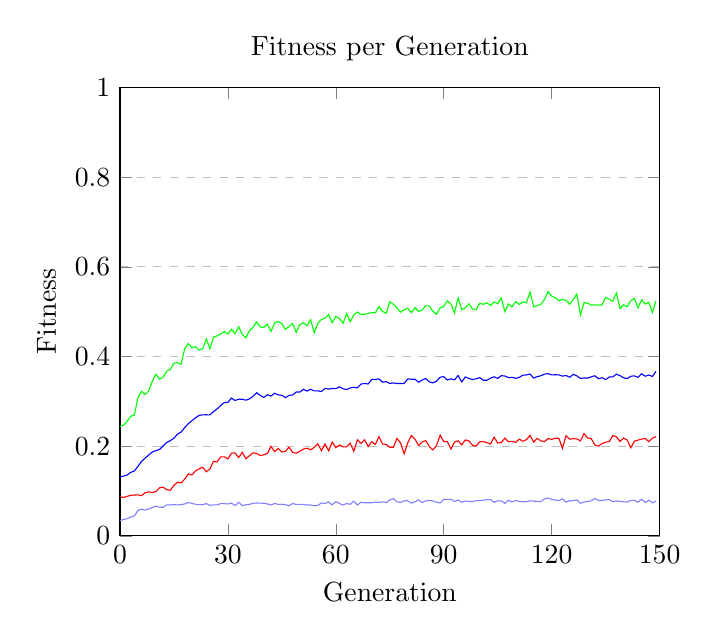
\begin{tikzpicture}
\begin{axis}[
	title={Fitness per Generation},
	xlabel={Generation},
	ylabel={Fitness},
	xmin=0, xmax=150,
	ymin=0, ymax=1,
	xtick={0.0,30.0,60.0,90.0,120.0,150.0},
	ytick={0.0,0.2,0.4,0.6000000000000001,0.8,1.0},
	ymajorgrids=true,
	grid style=dashed,
]

\addplot[
	color=green,
	]
	coordinates {
	(0,0.2441430555555556)(1,0.24682777777777773)(2,0.2556844444444445)(3,0.2668408333333333)(4,0.26971194444444446)(5,0.3082621296296296)(6,0.3225826851851852)(7,0.31531055555555554)(8,0.3234491666666667)(9,0.34532611111111117)(10,0.36060129629629634)(11,0.34978851851851867)(12,0.3540337962962963)(13,0.3677262962962963)(14,0.3710710185185184)(15,0.38529361111111105)(16,0.3862841666666667)(17,0.38283925925925927)(18,0.41752462962962966)(19,0.428976111111111)(20,0.419823611111111)(21,0.421965)(22,0.4143839814814814)(23,0.4174908333333332)(24,0.4393206481481482)(25,0.4172834259259259)(26,0.44312101851851865)(27,0.44617611111111116)(28,0.4506470370370371)(29,0.455871388888889)(30,0.45049601851851845)(31,0.4611457407407406)(32,0.4510065740740741)(33,0.46656907407407405)(34,0.4495473148148148)(35,0.44169018518518527)(36,0.4574708333333333)(37,0.46540203703703703)(38,0.4773607407407407)(39,0.46555148148148146)(40,0.4654059259259259)(41,0.4722998148148148)(42,0.4559755555555555)(43,0.4753555555555556)(44,0.47817462962962964)(45,0.473502037037037)(46,0.4603316666666666)(47,0.46740694444444447)(48,0.47373814814814813)(49,0.45393231481481483)(50,0.471237962962963)(51,0.47523509259259245)(52,0.46876037037037027)(53,0.4822818518518518)(54,0.45335907407407405)(55,0.4741485185185186)(56,0.48286453703703697)(57,0.48590611111111115)(58,0.49384083333333334)(59,0.47535546296296305)(60,0.48990787037037037)(61,0.48489407407407414)(62,0.4741303703703705)(63,0.49583759259259264)(64,0.4776655555555556)(65,0.49271027777777787)(66,0.49949787037037047)(67,0.49384138888888895)(68,0.49445592592592597)(69,0.49617870370370365)(70,0.49817138888888884)(71,0.49766046296296296)(72,0.5113411111111111)(73,0.500651574074074)(74,0.4965871296296296)(75,0.5223609259259259)(76,0.5165574999999999)(77,0.5084306481481481)(78,0.49899462962962954)(79,0.5046119444444445)(80,0.5079146296296296)(81,0.4980151851851852)(82,0.5090812037037037)(83,0.5009174999999999)(84,0.503929351851852)(85,0.5132300925925927)(86,0.5127416666666667)(87,0.5010292592592592)(88,0.49425518518518524)(89,0.5086314814814815)(90,0.511398888888889)(91,0.524597037037037)(92,0.5172125925925926)(93,0.4972375000000001)(94,0.53113)(95,0.5044247222222222)(96,0.5085783333333334)(97,0.517645925925926)(98,0.5060715740740741)(99,0.5048063888888888)(100,0.5189533333333334)(101,0.5166016666666667)(102,0.5198737962962963)(103,0.5137926851851853)(104,0.5216055555555557)(105,0.5181823148148148)(106,0.5300853703703704)(107,0.5000392592592592)(108,0.517411574074074)(109,0.5108712037037038)(110,0.5224427777777777)(111,0.5162531481481482)(112,0.5219337037037036)(113,0.5200362037037036)(114,0.5439453703703704)(115,0.5112422222222222)(116,0.5135154629629629)(117,0.5163411111111111)(118,0.5269914814814816)(119,0.5446783333333334)(120,0.5349224074074074)(121,0.5311508333333333)(122,0.5245001851851853)(123,0.5273876851851852)(124,0.5254970370370372)(125,0.5165710185185185)(126,0.5274259259259261)(127,0.5393774074074075)(128,0.4926662962962964)(129,0.5202709259259259)(130,0.5191621296296296)(131,0.5145357407407408)(132,0.51537)(133,0.5146901851851851)(134,0.5150850000000001)(135,0.5321728703703704)(136,0.5276329629629629)(137,0.5234199074074074)(138,0.5417262037037037)(139,0.5070412962962964)(140,0.515358611111111)(141,0.5112061111111111)(142,0.5245323148148148)(143,0.5296587962962963)(144,0.50847)(145,0.5266644444444445)(146,0.5169488888888889)(147,0.5211596296296296)(148,0.49827888888888894)(149,0.5247004629629629)
	};
\addplot[
	color=blue,
	]
	coordinates {
	(0,0.13127846836419754)(1,0.1333747222222222)(2,0.13608741512345676)(3,0.14161955246913582)(4,0.14477288966049381)(5,0.1549582986111111)(6,0.16614708333333333)(7,0.17363413194444444)(8,0.18044368441358022)(9,0.18717145061728396)(10,0.19019156250000002)(11,0.1927088927469136)(12,0.2007640162037037)(13,0.20846334104938274)(14,0.21231795138888887)(15,0.21793449459876543)(16,0.22693515432098763)(17,0.23160451774691357)(18,0.2415812538580247)(19,0.25033516203703704)(20,0.256929537037037)(21,0.2633461766975309)(22,0.26881819830246917)(23,0.27001010416666665)(24,0.2701377160493827)(25,0.2698841473765432)(26,0.2772451003086419)(27,0.2831779591049382)(28,0.2908057214506173)(29,0.29732459104938275)(30,0.2977862422839507)(31,0.30727340663580244)(32,0.30207204089506173)(33,0.30474680555555556)(34,0.304740837191358)(35,0.30273066743827165)(36,0.3056308179012346)(37,0.31132324845679016)(38,0.3194544714506173)(39,0.31339081018518516)(40,0.30880822916666667)(41,0.31473314043209877)(42,0.31197343750000006)(43,0.31816760030864205)(44,0.314485574845679)(45,0.3135336111111111)(46,0.3083695717592593)(47,0.31332795524691354)(48,0.31438388117283955)(49,0.3209832908950617)(50,0.3207781250000001)(51,0.3268402816358025)(52,0.3230580285493827)(53,0.3271507021604938)(54,0.3233232831790124)(55,0.3236285455246914)(56,0.3220001195987654)(57,0.3288203780864198)(58,0.3274999035493827)(59,0.3288696527777778)(60,0.3284621836419754)(61,0.3324014236111112)(62,0.3281960223765432)(63,0.32638072530864193)(64,0.3299133140432099)(65,0.331514899691358)(66,0.33022265046296295)(67,0.338652488425926)(68,0.3399830671296296)(69,0.33881986111111106)(70,0.34908076388888887)(71,0.3490523842592593)(72,0.350279637345679)(73,0.34270211419753077)(74,0.3440252199074074)(75,0.3400651890432099)(76,0.3410836033950618)(77,0.3399348225308643)(78,0.3398956828703704)(79,0.3400863155864197)(80,0.35027839120370363)(81,0.34946490740740743)(82,0.34939836805555563)(83,0.34274479552469134)(84,0.3476821797839506)(85,0.3512834606481482)(86,0.3434785841049383)(87,0.34124378086419754)(88,0.3450586265432099)(89,0.35398214891975305)(90,0.3550880979938271)(91,0.34767659336419754)(92,0.3503979050925926)(93,0.348011087962963)(94,0.35771145447530867)(95,0.3435729822530864)(96,0.35448888503086423)(97,0.3511472106481481)(98,0.34871958333333336)(99,0.3504243402777777)(100,0.3530512577160494)(101,0.34719766203703706)(102,0.34712371527777774)(103,0.35165174768518515)(104,0.35484258101851845)(105,0.3512418016975308)(106,0.3572960108024691)(107,0.3566915972222222)(108,0.3530711728395062)(109,0.3535107831790123)(110,0.35149434799382717)(111,0.3537671489197531)(112,0.35841792052469135)(113,0.359072712191358)(114,0.36087368441358014)(115,0.35199880787037036)(116,0.3553720601851852)(117,0.3571418981481482)(118,0.36077617283950614)(119,0.36191393904320984)(120,0.3590803665123457)(121,0.3594515470679012)(122,0.3590792669753086)(123,0.3563858757716049)(124,0.3577250694444444)(125,0.3536795408950617)(126,0.3603565740740741)(127,0.35689125)(128,0.3512367168209876)(129,0.35216902391975313)(130,0.3521456018518519)(131,0.3546637808641976)(132,0.357209375)(133,0.35054763117283955)(134,0.3529041936728396)(135,0.3485195949074075)(136,0.354331361882716)(137,0.354703074845679)(138,0.3607946720679012)(139,0.3574038811728395)(140,0.3526259259259259)(141,0.3508932137345679)(142,0.35606215277777775)(143,0.3569487037037038)(144,0.3535136265432099)(145,0.3613897415123457)(146,0.35616597222222224)(147,0.35880001157407404)(148,0.35556418595679007)(149,0.366934837962963)
	};
\addplot[
	color=red,
	]
	coordinates {
	(0,0.08747935185185185)(1,0.08578907407407409)(2,0.08821074074074071)(3,0.09046972222222216)(4,0.09113379629629632)(5,0.09147620370370373)(6,0.08970175925925924)(7,0.09625555555555555)(8,0.09821000000000002)(9,0.09649907407407407)(10,0.09917148148148144)(11,0.10732962962962962)(12,0.10860935185185182)(13,0.10304814814814815)(14,0.10162379629629632)(15,0.11279898148148149)(16,0.11946990740740739)(17,0.11808453703703704)(18,0.12658685185185187)(19,0.13820509259259253)(20,0.135730925925926)(21,0.1449135185185185)(22,0.14950694444444437)(23,0.15319120370370376)(24,0.1430002777777778)(25,0.1495432407407407)(26,0.1663436111111111)(27,0.16489444444444445)(28,0.17608222222222225)(29,0.17627351851851852)(30,0.17182861111111114)(31,0.18462472222222223)(32,0.185029537037037)(33,0.1746507407407408)(34,0.18639277777777777)(35,0.17223675925925927)(36,0.17884425925925923)(37,0.1852830555555556)(38,0.1838048148148148)(39,0.17938231481481484)(40,0.18089185185185191)(41,0.18407157407407407)(42,0.19966851851851847)(43,0.18805388888888888)(44,0.1951181481481482)(45,0.1871653703703704)(46,0.18870435185185183)(47,0.19806231481481482)(48,0.18628768518518513)(49,0.18437481481481477)(50,0.18907212962962963)(51,0.19351296296296297)(52,0.19561740740740746)(53,0.19217296296296305)(54,0.19722351851851852)(55,0.20559648148148155)(56,0.18984398148148152)(57,0.20504148148148146)(58,0.18962916666666663)(59,0.20921824074074072)(60,0.19670222222222217)(61,0.20273601851851858)(62,0.19849259259259264)(63,0.1987068518518518)(64,0.20684398148148148)(65,0.18855685185185178)(66,0.21436222222222223)(67,0.20659916666666667)(68,0.21413712962962966)(69,0.199110462962963)(70,0.20995268518518523)(71,0.2041217592592593)(72,0.22145814814814815)(73,0.2049467592592592)(74,0.20389398148148152)(75,0.1975588888888889)(76,0.19763277777777777)(77,0.2173712962962963)(78,0.20722324074074078)(79,0.18325416666666666)(80,0.20768814814814815)(81,0.22387370370370382)(82,0.21614796296296301)(83,0.20165314814814814)(84,0.20935703703703704)(85,0.2129622222222222)(86,0.19903759259259263)(87,0.1918175925925926)(88,0.20153361111111107)(89,0.22456500000000001)(90,0.21047361111111101)(91,0.21050046296296293)(92,0.19372324074074082)(93,0.20925898148148145)(94,0.2120040740740741)(95,0.202965462962963)(96,0.21403749999999996)(97,0.2118236111111111)(98,0.20205037037037032)(99,0.20051259259259252)(100,0.20983546296296302)(101,0.21033462962962962)(102,0.20801861111111108)(103,0.204965)(104,0.22027222222222226)(105,0.20724212962962973)(106,0.20844453703703708)(107,0.21798416666666665)(108,0.2098821296296296)(109,0.21094222222222228)(110,0.2085760185185185)(111,0.21584000000000006)(112,0.21099148148148145)(113,0.21485879629629626)(114,0.22412972222222227)(115,0.2092285185185185)(116,0.21751379629629625)(117,0.21185722222222225)(118,0.2104523148148148)(119,0.21718601851851846)(120,0.21525731481481486)(121,0.217705)(122,0.21776759259259254)(123,0.1953724074074074)(124,0.22369092592592596)(125,0.21566166666666658)(126,0.21696999999999994)(127,0.21612)(128,0.2119396296296296)(129,0.22822962962962962)(130,0.21824611111111122)(131,0.21695018518518513)(132,0.20272018518518517)(133,0.20000666666666675)(134,0.20603833333333332)(135,0.20892129629629633)(136,0.21046305555555558)(137,0.2236623148148148)(138,0.2209992592592593)(139,0.2106548148148148)(140,0.2182756481481482)(141,0.2136969444444445)(142,0.19644138888888887)(143,0.2113913888888889)(144,0.21362416666666664)(145,0.21579740740740747)(146,0.2172712037037037)(147,0.2104859259259259)(148,0.21816287037037035)(149,0.22118490740740743)
	};
\addplot[
	color=blue!50,
	]
	coordinates {
	(0,0.03413586961051367)(1,0.0365671984073854)(2,0.03849898573960934)(3,0.04197659249769223)(4,0.044500014957003724)(5,0.056633410519081495)(6,0.05937590061442925)(7,0.05759558079046282)(8,0.06007141406316464)(9,0.0629514965616286)(10,0.06640546734188198)(11,0.0640354013611381)(12,0.06383769225877471)(13,0.06909600710452217)(14,0.068978050442231)(15,0.06978293476952112)(16,0.0690750422687728)(17,0.06974505855121801)(18,0.07132492434238859)(19,0.07440309457268642)(20,0.07253752255743234)(21,0.07036672541234817)(22,0.06970259225052895)(23,0.06953821035717854)(24,0.07219341967366243)(25,0.06807538691685347)(26,0.06924577575019156)(27,0.06910949246620296)(28,0.07188053884317172)(29,0.07182121376794272)(30,0.07120400027034733)(31,0.07323250475577352)(32,0.06750885707182232)(33,0.07495000722725546)(34,0.06744023135171469)(35,0.06941074637611783)(36,0.07031945780649067)(37,0.0726216570528628)(38,0.07338145614828899)(39,0.07304114184100113)(40,0.07281639990709848)(41,0.07116315605617554)(42,0.06891735220031213)(43,0.07230585384883134)(44,0.07036690961659178)(45,0.07048884377995819)(46,0.06974618216088835)(47,0.06710954333799245)(48,0.07221920616289212)(49,0.07015303650103498)(50,0.07035238607614512)(51,0.07032899122419742)(52,0.06867883775195147)(53,0.06906602875997155)(54,0.06705812819933639)(55,0.06826992659338442)(56,0.07326818397644906)(57,0.07251806635807968)(58,0.0754525166735892)(59,0.06919497278158097)(60,0.07633736469539824)(61,0.07247212467193542)(62,0.06872839459498188)(63,0.07240427524560283)(64,0.07044187356893224)(65,0.07734839940848882)(66,0.06893582896722762)(67,0.07516925506220869)(68,0.07383017296732089)(69,0.0739026900709543)(70,0.07403409196726676)(71,0.07556172266151953)(72,0.07440767971258704)(73,0.07601312945585773)(74,0.07397588789400658)(75,0.08024353229360587)(76,0.08306867957793532)(77,0.07599539860553499)(78,0.07460338277826942)(79,0.07824875939503924)(80,0.07833568479011829)(81,0.07305219457170964)(82,0.07581642467070994)(83,0.08057993508789517)(84,0.07427589316756789)(85,0.07803694330966027)(86,0.07928837803359637)(87,0.07784022971899908)(88,0.07517542648496264)(89,0.07334490671003518)(90,0.08188702969010442)(91,0.08107755785404094)(92,0.08176945105351792)(93,0.07679278423279216)(94,0.07983049059427348)(95,0.07517438830712489)(96,0.0776371330631039)(97,0.07695284848234168)(98,0.07634643407179227)(99,0.07876950805090008)(100,0.07880618145520644)(101,0.07952800736319034)(102,0.0809309688497334)(103,0.08095951777195316)(104,0.07483260517096527)(105,0.07830445553723211)(106,0.07810592705862222)(107,0.07268475694763099)(108,0.07961316807287629)(109,0.07570613028822226)(110,0.07895540029086244)(111,0.07688796562528746)(112,0.07614277251337234)(113,0.07644379210981177)(114,0.07832911966043837)(115,0.0774014043738445)(116,0.07708581485451221)(117,0.07643814122360718)(118,0.08258452241993577)(119,0.08437330671117521)(120,0.0813798377374968)(121,0.08005506510286625)(122,0.07849926527987672)(123,0.08256465176904132)(124,0.07546010100271121)(125,0.07834941374540125)(126,0.07880511842526564)(127,0.08024552585957057)(128,0.07268467374464359)(129,0.07559637765809654)(130,0.07674477892458695)(131,0.0781729248441479)(132,0.0831174488330373)(133,0.07913322459272627)(134,0.07893106618391725)(135,0.08026240194779075)(136,0.0810834784642632)(137,0.07623485876452132)(138,0.07813889628514975)(139,0.07694681128680762)(140,0.07600424004175738)(141,0.07546922086369719)(142,0.07910120959612868)(143,0.07927043677779962)(144,0.075165331085765)(145,0.08176949606382307)(146,0.07427767353150186)(147,0.07955233814558915)(148,0.07373065206231608)(149,0.07745120735391954)
	};
\end{axis}
\end{tikzpicture}
}
		\caption{Some sample caption}
	\end{subfigure}%
}
\caption{Figure shows results from a simulation in the hard environment (p.1)}
\end{figure}

\newpage
\vspace*{-2.0cm}
\textbf{\Huge Results - Hard environment (2)}
\vspace{1.5cm}
\begin{tikzpicture}[remember picture,overlay]
   \node[anchor=south east,inner sep=20pt] at (current page.south east)
              {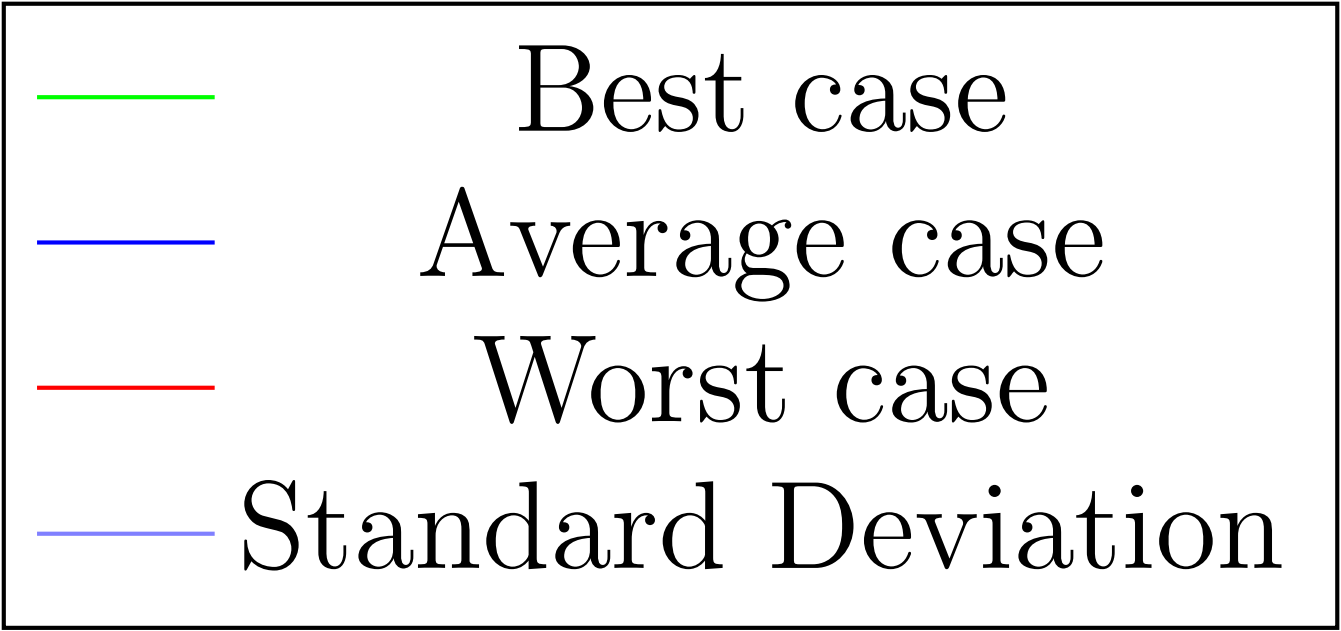
\includegraphics[scale=0.1]{chapters/res/generated_graph_legend.png}};
\end{tikzpicture}

\begin{figure}[H]
\vspace*{-1cm}
	\makebox[\linewidth][c]{%
	\begin{subfigure}[b]{0.7\textwidth}
		\centering
		\resizebox{0.9\linewidth}{!}{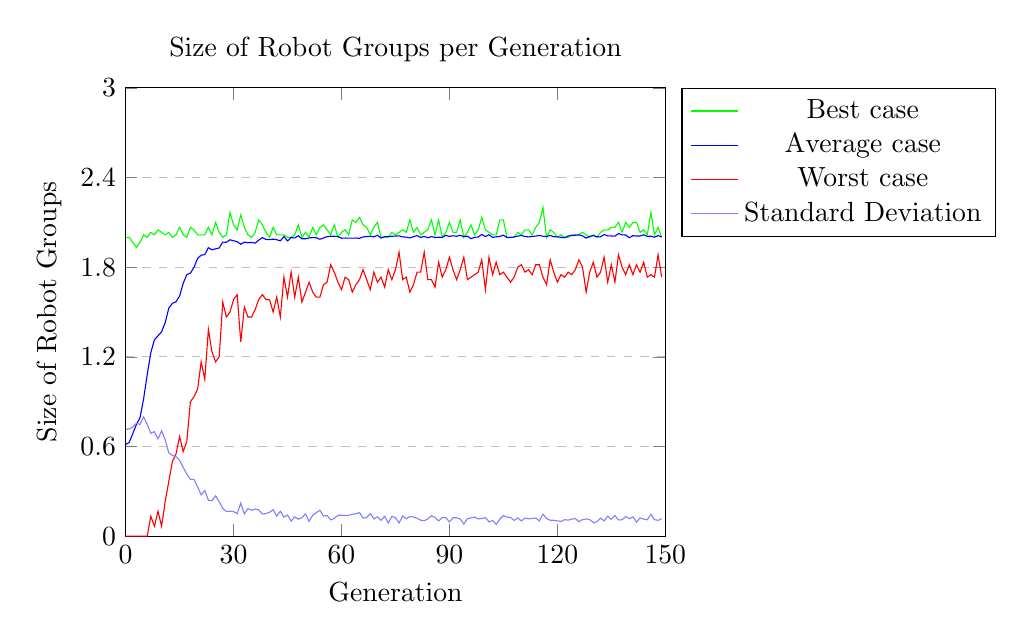
\begin{tikzpicture}
\begin{axis}[
	title={Size of Robot Groups per Generation},
	xlabel={Generation},
	ylabel={Size of Robot Groups},
	xmin=0, xmax=150,
	ymin=0, ymax=3,
	xtick={0.0,30.0,60.0,90.0,120.0,150.0},
	ytick={0.0,0.6,1.2,1.7999999999999998,2.4,3.0},
	legend pos=outer north east,
	ymajorgrids=true,
	grid style=dashed,
]

\addplot[
	color=green,
	]
	coordinates {
	(0,2.0000000000000004)(1,2.0000000000000004)(2,1.9666666666666672)(3,1.933333333333334)(4,1.9666666666666675)(5,2.016666666666667)(6,2.0000000000000004)(7,2.0333333333333337)(8,2.016666666666667)(9,2.0500000000000003)(10,2.0333333333333337)(11,2.016666666666667)(12,2.0333333333333337)(13,2.0000000000000004)(14,2.0166666666666675)(15,2.066666666666667)(16,2.016666666666667)(17,2.0000000000000004)(18,2.0666666666666673)(19,2.0500000000000003)(20,2.0166666666666675)(21,2.0166666666666675)(22,2.016666666666667)(23,2.0666666666666673)(24,2.0166666666666675)(25,2.1000000000000005)(26,2.033333333333334)(27,2.0000000000000004)(28,2.0166666666666675)(29,2.1666666666666674)(30,2.083333333333334)(31,2.0500000000000003)(32,2.1500000000000004)(33,2.0666666666666673)(34,2.016666666666667)(35,2.0000000000000004)(36,2.033333333333334)(37,2.116666666666667)(38,2.083333333333334)(39,2.033333333333334)(40,2.0000000000000004)(41,2.0666666666666673)(42,2.016666666666667)(43,2.0166666666666675)(44,2.0166666666666675)(45,2.0000000000000004)(46,2.0000000000000004)(47,2.016666666666667)(48,2.083333333333334)(49,2.0000000000000004)(50,2.033333333333334)(51,2.0000000000000004)(52,2.0666666666666673)(53,2.016666666666667)(54,2.066666666666667)(55,2.083333333333334)(56,2.0500000000000007)(57,2.016666666666667)(58,2.083333333333334)(59,2.0000000000000004)(60,2.033333333333334)(61,2.0500000000000003)(62,2.016666666666667)(63,2.116666666666667)(64,2.1000000000000005)(65,2.1333333333333337)(66,2.083333333333334)(67,2.0666666666666673)(68,2.0166666666666675)(69,2.0666666666666673)(70,2.1000000000000005)(71,2.0000000000000004)(72,2.0000000000000004)(73,2.0000000000000004)(74,2.033333333333334)(75,2.0166666666666675)(76,2.0333333333333337)(77,2.0500000000000007)(78,2.033333333333334)(79,2.116666666666667)(80,2.033333333333334)(81,2.0666666666666673)(82,2.0166666666666675)(83,2.033333333333334)(84,2.0500000000000007)(85,2.116666666666667)(86,2.016666666666667)(87,2.116666666666667)(88,2.0000000000000004)(89,2.033333333333334)(90,2.1000000000000005)(91,2.033333333333334)(92,2.033333333333334)(93,2.116666666666667)(94,2.0000000000000004)(95,2.033333333333334)(96,2.083333333333334)(97,2.0166666666666675)(98,2.0500000000000007)(99,2.1333333333333337)(100,2.0500000000000007)(101,2.033333333333334)(102,2.0166666666666675)(103,2.0166666666666675)(104,2.116666666666667)(105,2.116666666666667)(106,2.0000000000000004)(107,2.0000000000000004)(108,2.0000000000000004)(109,2.033333333333334)(110,2.0166666666666675)(111,2.0500000000000007)(112,2.0500000000000007)(113,2.0166666666666675)(114,2.0666666666666673)(115,2.1000000000000005)(116,2.2)(117,2.0000000000000004)(118,2.0500000000000007)(119,2.0333333333333337)(120,2.0000000000000004)(121,2.0166666666666675)(122,2.0000000000000004)(123,2.0000000000000004)(124,2.016666666666667)(125,2.0166666666666675)(126,2.016666666666667)(127,2.033333333333334)(128,2.016666666666667)(129,2.0000000000000004)(130,2.0166666666666675)(131,2.0000000000000004)(132,2.0333333333333337)(133,2.0500000000000007)(134,2.0500000000000007)(135,2.0666666666666673)(136,2.0666666666666673)(137,2.1000000000000005)(138,2.0333333333333337)(139,2.1000000000000005)(140,2.0666666666666673)(141,2.1000000000000005)(142,2.1000000000000005)(143,2.033333333333334)(144,2.0500000000000003)(145,2.016666666666667)(146,2.1666666666666674)(147,2.016666666666667)(148,2.0666666666666673)(149,2.0000000000000004)
	};
	\addlegendentry{Best case}
\addplot[
	color=blue,
	]
	coordinates {
	(0,0.6131944444444445)(1,0.6277777777777779)(2,0.6868055555555556)(3,0.7479166666666666)(4,0.7930555555555555)(5,0.9194444444444444)(6,1.0812499999999996)(7,1.2284722222222222)(8,1.313888888888889)(9,1.340972222222222)(10,1.3680555555555554)(11,1.4291666666666667)(12,1.526388888888889)(13,1.5583333333333333)(14,1.5687500000000003)(15,1.6069444444444447)(16,1.692361111111111)(17,1.7499999999999998)(18,1.760416666666667)(19,1.7986111111111112)(20,1.8590277777777782)(21,1.8805555555555555)(22,1.8840277777777779)(23,1.9305555555555558)(24,1.9159722222222226)(25,1.9229166666666668)(26,1.9284722222222224)(27,1.9680555555555554)(28,1.9666666666666672)(29,1.9833333333333336)(30,1.9770833333333337)(31,1.971527777777778)(32,1.9534722222222225)(33,1.9680555555555561)(34,1.963888888888889)(35,1.9659722222222227)(36,1.9611111111111117)(37,1.9812500000000004)(38,1.9979166666666672)(39,1.9861111111111118)(40,1.9847222222222225)(41,1.9875000000000005)(42,1.9840277777777784)(43,1.9763888888888894)(44,2.0048611111111114)(45,1.9756944444444449)(46,1.9979166666666668)(47,1.9958333333333338)(48,2.010416666666667)(49,1.990277777777778)(50,1.990277777777778)(51,1.9958333333333336)(52,1.9979166666666672)(53,1.9972222222222227)(54,1.9868055555555553)(55,1.9958333333333338)(56,2.0041666666666673)(57,2.0069444444444446)(58,2.0069444444444446)(59,2.0055555555555555)(60,1.9937500000000004)(61,1.9951388888888892)(62,1.994444444444445)(63,1.9944444444444447)(64,1.9951388888888892)(65,1.993055555555556)(66,2.002777777777778)(67,2.0048611111111114)(68,2.0069444444444446)(69,2.0034722222222223)(70,2.0138888888888893)(71,1.9951388888888895)(72,2.0048611111111114)(73,2.004861111111112)(74,2.0069444444444446)(75,2.0083333333333337)(76,2.0097222222222224)(77,2.002777777777778)(78,2.001388888888889)(79,1.9958333333333336)(80,2.004166666666667)(81,2.011805555555556)(82,1.999305555555556)(83,2.005555555555556)(84,1.9965277777777783)(85,2.0048611111111114)(86,1.9986111111111118)(87,2.000694444444445)(88,1.9986111111111116)(89,2.0131944444444447)(90,2.0062500000000005)(91,2.010416666666667)(92,2.006944444444445)(93,2.0138888888888893)(94,2.0041666666666664)(95,2.0076388888888888)(96,1.9909722222222224)(97,2.0000000000000004)(98,2.002083333333333)(99,2.019444444444445)(100,2.0048611111111114)(101,2.017361111111111)(102,1.9993055555555561)(103,2.0034722222222223)(104,2.005555555555556)(105,2.0145833333333334)(106,1.9986111111111116)(107,1.9993055555555557)(108,2.002777777777778)(109,2.007638888888889)(110,2.0125000000000006)(111,2.0055555555555555)(112,2.002777777777778)(113,2.005555555555556)(114,2.0083333333333337)(115,2.0131944444444447)(116,2.0069444444444446)(117,2.0048611111111114)(118,2.0125000000000006)(119,2.0041666666666673)(120,2.002777777777778)(121,2.0000000000000004)(122,1.9972222222222227)(123,2.0090277777777774)(124,2.0118055555555556)(125,2.0138888888888893)(126,2.0159722222222225)(127,2.0097222222222224)(128,1.994444444444445)(129,2.006944444444445)(130,2.0111111111111115)(131,2.0041666666666673)(132,2.002777777777778)(133,2.019444444444445)(134,2.009722222222223)(135,2.0090277777777783)(136,2.007638888888889)(137,2.025)(138,2.016666666666667)(139,2.015277777777778)(140,1.997222222222223)(141,2.0111111111111115)(142,2.0083333333333337)(143,2.0090277777777783)(144,2.016666666666667)(145,2.00625)(146,2.007638888888889)(147,2.0006944444444446)(148,2.011805555555556)(149,2.002083333333334)
	};
	\addlegendentry{Average case}
\addplot[
	color=red,
	]
	coordinates {
	(0,0.0)(1,0.0)(2,0.0)(3,0.0)(4,0.0)(5,0.0)(6,0.0)(7,0.13333333333333333)(8,0.06666666666666667)(9,0.16666666666666666)(10,0.06666666666666667)(11,0.23333333333333334)(12,0.36666666666666664)(13,0.49999999999999994)(14,0.5499999999999999)(15,0.6666666666666666)(16,0.5666666666666667)(17,0.6333333333333333)(18,0.8999999999999999)(19,0.9333333333333332)(20,0.9833333333333333)(21,1.1666666666666667)(22,1.05)(23,1.3833333333333337)(24,1.2333333333333334)(25,1.1666666666666667)(26,1.2000000000000002)(27,1.566666666666667)(28,1.4666666666666668)(29,1.5000000000000002)(30,1.5833333333333335)(31,1.6166666666666671)(32,1.3)(33,1.5333333333333339)(34,1.4666666666666668)(35,1.4666666666666668)(36,1.5166666666666668)(37,1.5833333333333335)(38,1.6166666666666671)(39,1.5833333333333335)(40,1.5833333333333335)(41,1.5000000000000002)(42,1.6)(43,1.4666666666666668)(44,1.7333333333333336)(45,1.6)(46,1.766666666666667)(47,1.6)(48,1.7333333333333338)(49,1.5666666666666667)(50,1.6333333333333335)(51,1.7000000000000002)(52,1.6333333333333335)(53,1.6000000000000003)(54,1.6000000000000005)(55,1.6833333333333336)(56,1.7000000000000004)(57,1.816666666666667)(58,1.766666666666667)(59,1.7000000000000002)(60,1.6500000000000001)(61,1.7333333333333336)(62,1.7166666666666668)(63,1.6333333333333335)(64,1.6833333333333336)(65,1.716666666666667)(66,1.7833333333333337)(67,1.7166666666666672)(68,1.6500000000000004)(69,1.766666666666667)(70,1.7000000000000002)(71,1.7333333333333336)(72,1.666666666666667)(73,1.7833333333333339)(74,1.716666666666667)(75,1.7833333333333337)(76,1.9000000000000004)(77,1.716666666666667)(78,1.7333333333333338)(79,1.6333333333333333)(80,1.6833333333333336)(81,1.766666666666667)(82,1.7666666666666668)(83,1.9000000000000006)(84,1.7166666666666668)(85,1.7166666666666668)(86,1.666666666666667)(87,1.833333333333334)(88,1.7333333333333338)(89,1.7833333333333337)(90,1.8666666666666671)(91,1.7833333333333337)(92,1.7166666666666668)(93,1.7833333333333337)(94,1.8666666666666671)(95,1.716666666666667)(96,1.7333333333333334)(97,1.7500000000000004)(98,1.766666666666667)(99,1.85)(100,1.6500000000000001)(101,1.8666666666666671)(102,1.7500000000000002)(103,1.833333333333334)(104,1.7500000000000004)(105,1.7666666666666668)(106,1.7333333333333338)(107,1.7000000000000002)(108,1.7333333333333336)(109,1.8000000000000005)(110,1.8166666666666669)(111,1.766666666666667)(112,1.7833333333333339)(113,1.7500000000000004)(114,1.816666666666667)(115,1.8166666666666669)(116,1.7333333333333336)(117,1.6833333333333336)(118,1.8500000000000005)(119,1.766666666666667)(120,1.7000000000000002)(121,1.7500000000000004)(122,1.7333333333333336)(123,1.766666666666667)(124,1.7500000000000004)(125,1.7833333333333337)(126,1.8500000000000003)(127,1.8000000000000005)(128,1.6333333333333335)(129,1.766666666666667)(130,1.833333333333334)(131,1.7333333333333336)(132,1.7666666666666668)(133,1.8666666666666671)(134,1.7000000000000002)(135,1.8166666666666669)(136,1.7000000000000002)(137,1.883333333333334)(138,1.8000000000000003)(139,1.7500000000000002)(140,1.816666666666667)(141,1.7500000000000004)(142,1.816666666666667)(143,1.766666666666667)(144,1.8333333333333337)(145,1.7333333333333336)(146,1.7500000000000004)(147,1.7333333333333338)(148,1.8833333333333337)(149,1.7333333333333336)
	};
	\addlegendentry{Worst case}
\addplot[
	color=blue!50,
	]
	coordinates {
	(0,0.7138361235782287)(1,0.7187262095445738)(2,0.7299017794351781)(3,0.7563808494297749)(4,0.747732439973878)(5,0.7989204112649962)(6,0.7476973173824782)(7,0.6888905403907576)(8,0.6995022331795739)(9,0.6505915757344015)(10,0.7059274760270886)(11,0.6438956492388662)(12,0.5575960349141993)(13,0.5406769248083867)(14,0.5324892948592459)(15,0.5079112053527064)(16,0.4599195856756785)(17,0.4164435106368284)(18,0.3796596155369205)(19,0.3798284372183864)(20,0.3305841911468127)(21,0.27672678058236605)(22,0.30553168074991116)(23,0.24107293353425632)(24,0.23758300093149337)(25,0.27037616427256783)(26,0.23060557330658668)(27,0.18635811027144492)(28,0.1654997458910107)(29,0.1669148179579515)(30,0.16464640290166058)(31,0.15092034546982896)(32,0.2212545791143057)(33,0.1491233233331111)(34,0.18540887115306037)(35,0.17357545648184913)(36,0.18165570746428678)(37,0.1756685870654313)(38,0.14781933253396337)(39,0.15185898466023437)(40,0.1600164368355709)(41,0.17746338436700668)(42,0.13475011998412478)(43,0.16689954134752075)(44,0.12827001407023395)(45,0.14141556363725508)(46,0.10064218964919368)(47,0.12948089434517165)(48,0.11369302198229254)(49,0.12392931621011408)(50,0.1493467708286089)(51,0.09959663938159165)(52,0.13991855575679604)(53,0.1573141009044969)(54,0.17340697081263295)(55,0.13517751822941343)(56,0.13790434537647742)(57,0.10921329007811643)(58,0.11884855689598224)(59,0.13970901931699564)(60,0.1401558016046057)(61,0.1380564647673069)(62,0.13911384923906187)(63,0.14676200864694958)(64,0.14933208363337042)(65,0.15815282327068197)(66,0.12091663709188709)(67,0.1253645943755902)(68,0.15148918957616692)(69,0.11583861114287937)(70,0.12941479785112944)(71,0.10633109429728797)(72,0.13359080336816367)(73,0.08890258481671645)(74,0.13235846069292498)(75,0.12403669804021311)(76,0.08818504377225796)(77,0.13477640829560206)(78,0.11634537323279837)(79,0.1314895784638423)(80,0.1285773151412238)(81,0.12014834767919261)(82,0.1072782561787095)(83,0.10349816085769578)(84,0.11535563509268716)(85,0.13685758095406497)(86,0.1262769885187133)(87,0.10207294170493016)(88,0.12522259860491122)(89,0.12327439150811799)(90,0.0958900752649856)(91,0.12307780364176674)(92,0.12310144392108487)(93,0.11551247892435162)(94,0.08036096849335571)(95,0.11597354288967975)(96,0.12219152184439537)(97,0.1274955742167325)(98,0.11519807834645783)(99,0.11840136171260857)(100,0.12433716384782328)(101,0.09600699671353308)(102,0.10558314244669247)(103,0.07928526440600364)(104,0.11346878651608108)(105,0.13791040838986304)(106,0.12756381020099816)(107,0.12535924370111418)(108,0.10523209902785492)(109,0.12262780975488223)(110,0.10171277480806264)(111,0.12131922255050326)(112,0.11583692932532819)(113,0.11865275151898305)(114,0.12139573416060899)(115,0.10223542564261373)(116,0.14790461910894107)(117,0.11814442897948943)(118,0.10685669854791247)(119,0.10624619656116596)(120,0.10244641388444574)(121,0.09913350753236683)(122,0.1101873943503501)(123,0.10757713547601122)(124,0.1141254843847288)(125,0.11824049361152743)(126,0.09746860160736023)(127,0.11068656861940362)(128,0.1154444641408269)(129,0.11119664383247747)(130,0.09033762334267456)(131,0.09687679440999944)(132,0.12138290023465188)(133,0.1018533223127771)(134,0.1337813070623874)(135,0.11236812590303351)(136,0.1384661566115684)(137,0.10852660114112964)(138,0.11001459958302398)(139,0.1316327713496007)(140,0.11706923351114477)(141,0.12948987532255687)(142,0.09393520068849275)(143,0.12217622865298865)(144,0.11426762685962104)(145,0.11025525444993266)(146,0.14658633290041953)(147,0.11054721555310816)(148,0.10629049017591466)(149,0.1173389105725204)
	};
	\addlegendentry{Standard Deviation}
\end{axis}
\end{tikzpicture}
}
		\caption{Some sample caption}
	\end{subfigure}%
	\begin{subfigure}[b]{0.7\textwidth}
		\centering
		\resizebox{0.9\linewidth}{!}{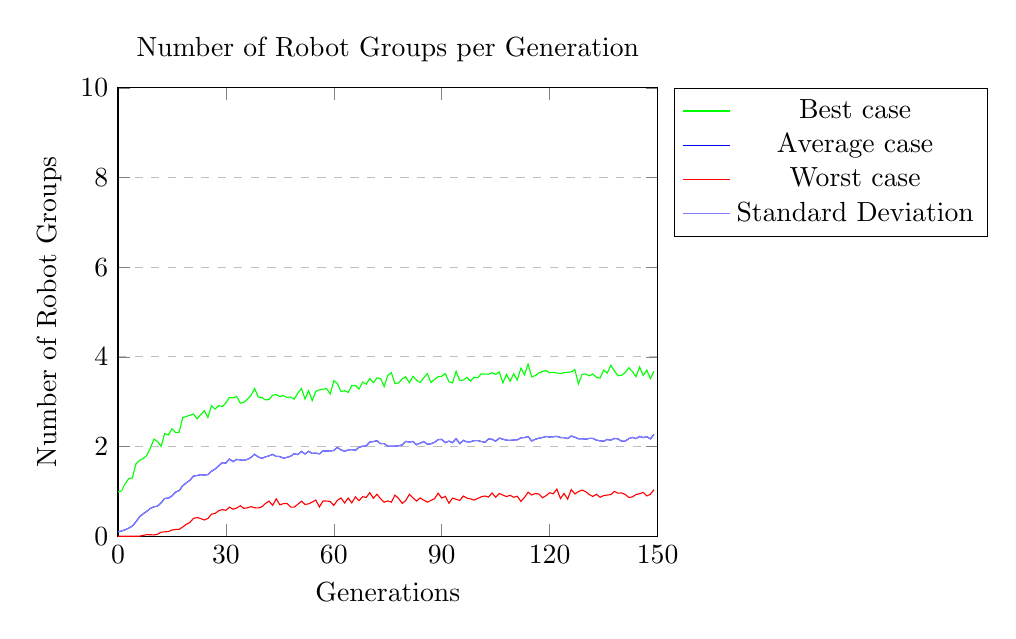
\begin{tikzpicture}
\begin{axis}[
	title={Number of Robot Groups per Generation},
	xlabel={Generations},
	ylabel={Number of Robot Groups},
	xmin=0, xmax=150,
	ymin=0, ymax=10,
	xtick={0.0,30.0,60.0,90.0,120.0,150.0},
	ytick={0.0,2.0,4.0,6.0,8.0,10.0},
	legend pos=outer north east,
	ymajorgrids=true,
	grid style=dashed,
]

\addplot[
	color=green,
	]
	coordinates {
	(0,0.9885)(1,1.0105)(2,1.1705)(3,1.2850833333333334)(4,1.3003333333333333)(5,1.6087499999999997)(6,1.6916666666666667)(7,1.73125)(8,1.8010000000000002)(9,1.96225)(10,2.1654166666666663)(11,2.1138333333333335)(12,2.0058333333333334)(13,2.290166666666667)(14,2.2583333333333333)(15,2.39425)(16,2.3168333333333333)(17,2.3175833333333338)(18,2.6443333333333334)(19,2.6715)(20,2.698166666666667)(21,2.7266666666666666)(22,2.616916666666667)(23,2.711)(24,2.8004999999999995)(25,2.647416666666666)(26,2.9100833333333336)(27,2.8361666666666667)(28,2.91375)(29,2.88775)(30,2.9744166666666665)(31,3.096333333333333)(32,3.0847500000000005)(33,3.1181666666666668)(34,2.9665)(35,2.987083333333333)(36,3.0541666666666663)(37,3.144833333333333)(38,3.293916666666667)(39,3.102416666666666)(40,3.094583333333333)(41,3.039833333333333)(42,3.0495)(43,3.1460000000000004)(44,3.1583333333333328)(45,3.1134999999999997)(46,3.13675)(47,3.0943333333333336)(48,3.1045833333333333)(49,3.0574166666666662)(50,3.1907499999999995)(51,3.2953333333333332)(52,3.060583333333334)(53,3.2466666666666666)(54,3.0235000000000003)(55,3.233416666666666)(56,3.2635000000000005)(57,3.27775)(58,3.2928333333333333)(59,3.170416666666666)(60,3.4700833333333327)(61,3.4057500000000003)(62,3.22525)(63,3.245166666666667)(64,3.2065833333333327)(65,3.360416666666667)(66,3.3628333333333327)(67,3.283583333333334)(68,3.4359166666666665)(69,3.3921666666666663)(70,3.5194166666666664)(71,3.4246666666666674)(72,3.5332500000000002)(73,3.5153333333333334)(74,3.3373333333333335)(75,3.5867500000000003)(76,3.647083333333333)(77,3.4069166666666666)(78,3.4181666666666666)(79,3.506250000000001)(80,3.5550000000000006)(81,3.42275)(82,3.566833333333333)(83,3.476333333333333)(84,3.427083333333333)(85,3.5321666666666665)(86,3.62825)(87,3.4285833333333327)(88,3.496833333333333)(89,3.559916666666667)(90,3.5672499999999996)(91,3.626749999999999)(92,3.4471666666666665)(93,3.418916666666667)(94,3.677583333333333)(95,3.4754166666666677)(96,3.48075)(97,3.5424166666666674)(98,3.4597500000000005)(99,3.5475000000000003)(100,3.536083333333333)(101,3.6227500000000004)(102,3.614583333333333)(103,3.613083333333334)(104,3.6454999999999993)(105,3.6109999999999993)(106,3.6636666666666673)(107,3.420416666666666)(108,3.6105)(109,3.4541666666666666)(110,3.6239999999999997)(111,3.48375)(112,3.747833333333334)(113,3.5999166666666667)(114,3.838333333333333)(115,3.554)(116,3.5820833333333333)(117,3.6424999999999996)(118,3.6724166666666664)(119,3.6955833333333343)(120,3.6435)(121,3.6565000000000007)(122,3.639166666666667)(123,3.6272500000000005)(124,3.649749999999999)(125,3.654166666666667)(126,3.6645833333333333)(127,3.7170833333333335)(128,3.397333333333333)(129,3.6089166666666666)(130,3.617083333333334)(131,3.5771666666666673)(132,3.6181666666666663)(133,3.54275)(134,3.5235)(135,3.704916666666667)(136,3.6390000000000002)(137,3.8111666666666664)(138,3.6860833333333334)(139,3.5785833333333334)(140,3.591083333333333)(141,3.6481666666666674)(142,3.7577500000000006)(143,3.671416666666667)(144,3.5568333333333335)(145,3.7747499999999996)(146,3.584916666666667)(147,3.7040833333333327)(148,3.5135)(149,3.674416666666666)
	};
	\addlegendentry{Best case}
\addplot[
	color=blue,
	]
	coordinates {
	(0,0.0986736111111111)(1,0.11563888888888892)(2,0.1426458333333333)(3,0.18130902777777777)(4,0.22395138888888888)(5,0.32067013888888884)(6,0.43254513888888896)(7,0.49868749999999995)(8,0.5538819444444445)(9,0.6199756944444443)(10,0.6553159722222224)(11,0.6706458333333334)(12,0.7433020833333333)(13,0.8430902777777779)(14,0.8488055555555555)(15,0.8977881944444445)(16,0.981670138888889)(17,1.0169166666666667)(18,1.1233020833333334)(19,1.18953125)(20,1.2479861111111112)(21,1.339875)(22,1.3537916666666665)(23,1.3705347222222222)(24,1.3649027777777778)(25,1.3736041666666663)(26,1.4487222222222222)(27,1.4972916666666665)(28,1.5694756944444443)(29,1.6386666666666667)(30,1.6303541666666668)(31,1.7230937499999999)(32,1.662611111111111)(33,1.712079861111111)(34,1.702982638888889)(35,1.6919722222222224)(36,1.7151874999999999)(37,1.7570520833333334)(38,1.827579861111111)(39,1.7665347222222223)(40,1.7368854166666665)(41,1.7686770833333334)(42,1.7917881944444443)(43,1.824125)(44,1.781965277777778)(45,1.776152777777778)(46,1.7410486111111105)(47,1.7593124999999998)(48,1.7837604166666667)(49,1.8403402777777778)(50,1.8206562499999999)(51,1.8905277777777778)(52,1.8341423611111114)(53,1.89275)(54,1.8469409722222223)(55,1.8537777777777777)(56,1.8366354166666665)(57,1.902451388888889)(58,1.8989236111111105)(59,1.9026631944444448)(60,1.9133194444444444)(61,1.9780381944444443)(62,1.9263368055555552)(63,1.8948888888888893)(64,1.9223298611111113)(65,1.931163194444444)(66,1.9163229166666667)(67,1.9829479166666664)(68,2.0066631944444446)(69,2.0135868055555557)(70,2.1003055555555554)(71,2.111045138888889)(72,2.12778125)(73,2.06596875)(74,2.0651805555555556)(75,2.0068402777777776)(76,2.0059027777777776)(77,2.008583333333333)(78,2.016284722222222)(79,2.034979166666667)(80,2.115166666666667)(81,2.1018298611111117)(82,2.1125659722222223)(83,2.0398645833333338)(84,2.0773993055555557)(85,2.1102499999999997)(86,2.0515000000000003)(87,2.0621666666666667)(88,2.0943125000000005)(89,2.1544409722222224)(90,2.157934027777778)(91,2.087427083333333)(92,2.1207604166666667)(93,2.0860347222222226)(94,2.175947916666667)(95,2.065892361111111)(96,2.1383576388888894)(97,2.1034548611111115)(98,2.1055868055555553)(99,2.1319270833333333)(100,2.1327881944444442)(101,2.1116354166666667)(102,2.093819444444444)(103,2.1682569444444444)(104,2.161482638888889)(105,2.119854166666667)(106,2.188097222222222)(107,2.1633472222222223)(108,2.1410104166666666)(109,2.137274305555555)(110,2.1465312500000002)(111,2.1476666666666664)(112,2.1951875)(113,2.199246527777778)(114,2.2231423611111114)(115,2.125541666666667)(116,2.1619826388888885)(117,2.186225694444444)(118,2.20009375)(119,2.224652777777777)(120,2.211857638888889)(121,2.2187812500000006)(122,2.227243055555556)(123,2.2010902777777774)(124,2.198652777777778)(125,2.1774444444444443)(126,2.2343993055555558)(127,2.208243055555556)(128,2.172427083333333)(129,2.1739618055555563)(130,2.164527777777778)(131,2.180510416666667)(132,2.180861111111111)(133,2.14246875)(134,2.127434027777778)(135,2.1188958333333328)(136,2.1578958333333333)(137,2.1426180555555554)(138,2.1806875)(139,2.1707534722222226)(140,2.118270833333333)(141,2.1218229166666664)(142,2.176100694444445)(143,2.204652777777778)(144,2.1769930555555557)(145,2.225496527777778)(146,2.1988090277777776)(147,2.219822916666667)(148,2.171017361111111)(149,2.2716458333333334)
	};
	\addlegendentry{Average case}
\addplot[
	color=red,
	]
	coordinates {
	(0,0.0)(1,0.0)(2,0.0)(3,0.0)(4,0.0)(5,0.0)(6,0.0)(7,0.018416666666666668)(8,0.033916666666666664)(9,0.032999999999999995)(10,0.027666666666666666)(11,0.043833333333333335)(12,0.08908333333333332)(13,0.09741666666666668)(14,0.10224999999999998)(15,0.13725)(16,0.1509166666666667)(17,0.1515)(18,0.20441666666666666)(19,0.2655833333333334)(20,0.30783333333333335)(21,0.3978333333333333)(22,0.41658333333333325)(23,0.39424999999999993)(24,0.36108333333333337)(25,0.3956666666666667)(26,0.4923333333333334)(27,0.5069999999999999)(28,0.5691666666666666)(29,0.59275)(30,0.5777500000000001)(31,0.6479999999999999)(32,0.6024166666666668)(33,0.6264166666666667)(34,0.6792499999999999)(35,0.6212500000000001)(36,0.63325)(37,0.6598333333333333)(38,0.6344166666666666)(39,0.6306666666666667)(40,0.6546666666666665)(41,0.7289999999999999)(42,0.7833333333333334)(43,0.6891666666666665)(44,0.8331666666666665)(45,0.7008333333333333)(46,0.7259166666666667)(47,0.7321666666666664)(48,0.6498333333333333)(49,0.6499999999999999)(50,0.7134166666666667)(51,0.7802499999999999)(52,0.7077500000000001)(53,0.7216666666666667)(54,0.7610833333333334)(55,0.8069166666666667)(56,0.6530833333333333)(57,0.7851666666666667)(58,0.78375)(59,0.7748333333333333)(60,0.6873333333333334)(61,0.8006666666666666)(62,0.8529166666666665)(63,0.7414166666666665)(64,0.8497500000000001)(65,0.7426666666666666)(66,0.8765833333333333)(67,0.7916666666666666)(68,0.8815000000000001)(69,0.8643333333333333)(70,0.9700833333333332)(71,0.8468333333333334)(72,0.936)(73,0.8344166666666667)(74,0.7593333333333332)(75,0.7856666666666666)(76,0.7581666666666667)(77,0.9169166666666665)(78,0.8422499999999999)(79,0.7321666666666667)(80,0.7949999999999999)(81,0.9334999999999999)(82,0.8554166666666665)(83,0.7841666666666668)(84,0.8524166666666667)(85,0.8040833333333332)(86,0.7609166666666667)(87,0.79725)(88,0.8359166666666668)(89,0.9601666666666667)(90,0.8495000000000001)(91,0.8886666666666665)(92,0.73475)(93,0.8495)(94,0.8240000000000001)(95,0.7965833333333333)(96,0.8959166666666666)(97,0.8487500000000001)(98,0.8320000000000001)(99,0.805)(100,0.8426666666666666)(101,0.8781666666666665)(102,0.8965)(103,0.8733333333333334)(104,0.9645833333333332)(105,0.8679166666666668)(106,0.95325)(107,0.9172500000000002)(108,0.8829166666666666)(109,0.9134166666666669)(110,0.8678333333333333)(111,0.893)(112,0.7754999999999999)(113,0.8655)(114,0.9804166666666667)(115,0.9194166666666667)(116,0.9515)(117,0.9411666666666667)(118,0.8586666666666664)(119,0.9035833333333334)(120,0.9685833333333335)(121,0.9459166666666666)(122,1.0505)(123,0.8401666666666664)(124,0.9539166666666667)(125,0.8270833333333335)(126,1.0401666666666665)(127,0.9424166666666667)(128,0.9944166666666667)(129,1.0269166666666667)(130,0.9955000000000003)(131,0.92825)(132,0.8865833333333333)(133,0.9358333333333333)(134,0.8685833333333333)(135,0.9058333333333333)(136,0.9175)(137,0.928)(138,1.0005000000000002)(139,0.9591666666666667)(140,0.96475)(141,0.9314166666666667)(142,0.86325)(143,0.8765833333333335)(144,0.9290833333333335)(145,0.94825)(146,0.9764166666666666)(147,0.8981666666666667)(148,0.9358333333333333)(149,1.0391666666666666)
	};
	\addlegendentry{Worst case}
\addplot[
	color=blue!50,
	]
	coordinates {
	(0,0.0986736111111111)(1,0.11563888888888892)(2,0.1426458333333333)(3,0.18130902777777777)(4,0.22395138888888888)(5,0.32067013888888884)(6,0.43254513888888896)(7,0.49868749999999995)(8,0.5538819444444445)(9,0.6199756944444443)(10,0.6553159722222224)(11,0.6706458333333334)(12,0.7433020833333333)(13,0.8430902777777779)(14,0.8488055555555555)(15,0.8977881944444445)(16,0.981670138888889)(17,1.0169166666666667)(18,1.1233020833333334)(19,1.18953125)(20,1.2479861111111112)(21,1.339875)(22,1.3537916666666665)(23,1.3705347222222222)(24,1.3649027777777778)(25,1.3736041666666663)(26,1.4487222222222222)(27,1.4972916666666665)(28,1.5694756944444443)(29,1.6386666666666667)(30,1.6303541666666668)(31,1.7230937499999999)(32,1.662611111111111)(33,1.712079861111111)(34,1.702982638888889)(35,1.6919722222222224)(36,1.7151874999999999)(37,1.7570520833333334)(38,1.827579861111111)(39,1.7665347222222223)(40,1.7368854166666665)(41,1.7686770833333334)(42,1.7917881944444443)(43,1.824125)(44,1.781965277777778)(45,1.776152777777778)(46,1.7410486111111105)(47,1.7593124999999998)(48,1.7837604166666667)(49,1.8403402777777778)(50,1.8206562499999999)(51,1.8905277777777778)(52,1.8341423611111114)(53,1.89275)(54,1.8469409722222223)(55,1.8537777777777777)(56,1.8366354166666665)(57,1.902451388888889)(58,1.8989236111111105)(59,1.9026631944444448)(60,1.9133194444444444)(61,1.9780381944444443)(62,1.9263368055555552)(63,1.8948888888888893)(64,1.9223298611111113)(65,1.931163194444444)(66,1.9163229166666667)(67,1.9829479166666664)(68,2.0066631944444446)(69,2.0135868055555557)(70,2.1003055555555554)(71,2.111045138888889)(72,2.12778125)(73,2.06596875)(74,2.0651805555555556)(75,2.0068402777777776)(76,2.0059027777777776)(77,2.008583333333333)(78,2.016284722222222)(79,2.034979166666667)(80,2.115166666666667)(81,2.1018298611111117)(82,2.1125659722222223)(83,2.0398645833333338)(84,2.0773993055555557)(85,2.1102499999999997)(86,2.0515000000000003)(87,2.0621666666666667)(88,2.0943125000000005)(89,2.1544409722222224)(90,2.157934027777778)(91,2.087427083333333)(92,2.1207604166666667)(93,2.0860347222222226)(94,2.175947916666667)(95,2.065892361111111)(96,2.1383576388888894)(97,2.1034548611111115)(98,2.1055868055555553)(99,2.1319270833333333)(100,2.1327881944444442)(101,2.1116354166666667)(102,2.093819444444444)(103,2.1682569444444444)(104,2.161482638888889)(105,2.119854166666667)(106,2.188097222222222)(107,2.1633472222222223)(108,2.1410104166666666)(109,2.137274305555555)(110,2.1465312500000002)(111,2.1476666666666664)(112,2.1951875)(113,2.199246527777778)(114,2.2231423611111114)(115,2.125541666666667)(116,2.1619826388888885)(117,2.186225694444444)(118,2.20009375)(119,2.224652777777777)(120,2.211857638888889)(121,2.2187812500000006)(122,2.227243055555556)(123,2.2010902777777774)(124,2.198652777777778)(125,2.1774444444444443)(126,2.2343993055555558)(127,2.208243055555556)(128,2.172427083333333)(129,2.1739618055555563)(130,2.164527777777778)(131,2.180510416666667)(132,2.180861111111111)(133,2.14246875)(134,2.127434027777778)(135,2.1188958333333328)(136,2.1578958333333333)(137,2.1426180555555554)(138,2.1806875)(139,2.1707534722222226)(140,2.118270833333333)(141,2.1218229166666664)(142,2.176100694444445)(143,2.204652777777778)(144,2.1769930555555557)(145,2.225496527777778)(146,2.1988090277777776)(147,2.219822916666667)(148,2.171017361111111)(149,2.2716458333333334)
	};
	\addlegendentry{Standard Deviation}
\end{axis}
\end{tikzpicture}
}
		\caption{Some sample caption}
	\end{subfigure}%
}
\\
\\
\\
\\
	\makebox[\linewidth][c]{%
	\begin{subfigure}[b]{0.7\textwidth}
		\centering
		\resizebox{0.9\linewidth}{!}{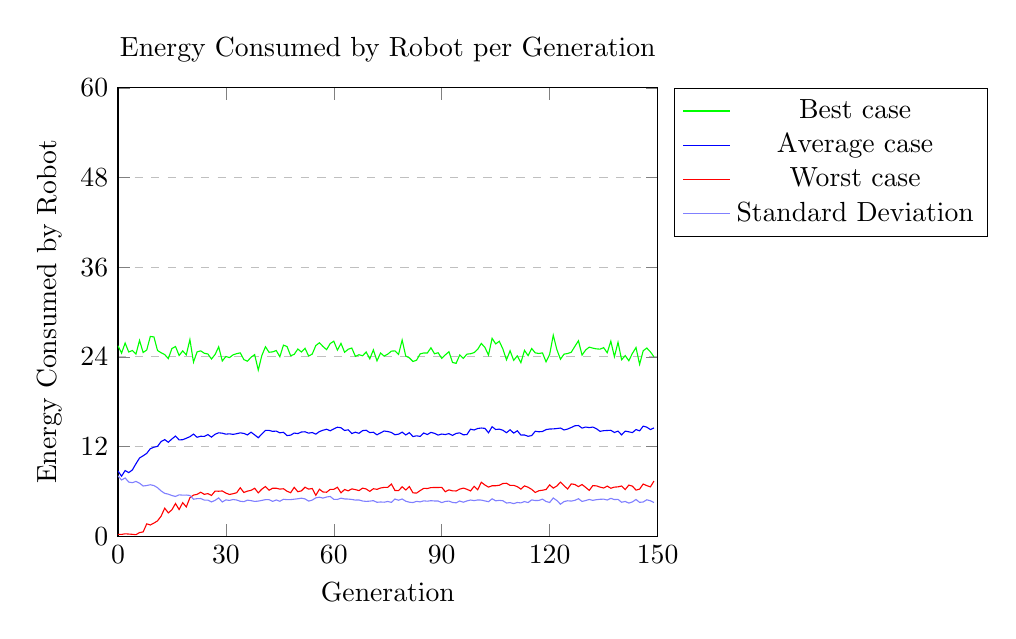
\begin{tikzpicture}
\begin{axis}[
	title={Energy Consumed by Robot per Generation},
	xlabel={Generation},
	ylabel={Energy Consumed by Robot},
	xmin=0, xmax=150,
	ymin=0, ymax=60,
	xtick={0.0,30.0,60.0,90.0,120.0,150.0},
	ytick={0.0,12.0,24.0,36.0,48.0,60.0},
	legend pos=outer north east,
	ymajorgrids=true,
	grid style=dashed,
]

\addplot[
	color=green,
	]
	coordinates {
	(0,25.5)(1,24.5)(2,25.850000000000005)(3,24.650000000000002)(4,24.849999999999998)(5,24.366666666666667)(6,26.199999999999996)(7,24.583333333333332)(8,24.916666666666664)(9,26.733333333333334)(10,26.666666666666664)(11,24.85)(12,24.55)(13,24.300000000000004)(14,23.766666666666666)(15,25.11666666666667)(16,25.38333333333333)(17,24.18333333333333)(18,24.800000000000004)(19,24.26666666666667)(20,26.316666666666663)(21,23.299999999999997)(22,24.666666666666664)(23,24.800000000000004)(24,24.48333333333333)(25,24.383333333333336)(26,23.716666666666672)(27,24.316666666666663)(28,25.350000000000005)(29,23.45)(30,24.05)(31,23.900000000000002)(32,24.26666666666667)(33,24.433333333333334)(34,24.533333333333328)(35,23.63333333333333)(36,23.416666666666668)(37,23.95)(38,24.3)(39,22.233333333333334)(40,24.18333333333333)(41,25.35)(42,24.616666666666664)(43,24.666666666666664)(44,24.849999999999998)(45,24.016666666666666)(46,25.566666666666663)(47,25.383333333333333)(48,24.150000000000002)(49,24.333333333333336)(50,25.05)(51,24.65)(52,25.150000000000002)(53,24.11666666666667)(54,24.36666666666667)(55,25.516666666666666)(56,25.88333333333333)(57,25.383333333333336)(58,24.96666666666667)(59,25.78333333333334)(60,26.100000000000005)(61,24.9)(62,25.799999999999997)(63,24.616666666666667)(64,25.016666666666666)(65,25.183333333333337)(66,24.066666666666666)(67,24.28333333333333)(68,24.15)(69,24.65)(70,23.733333333333334)(71,24.93333333333333)(72,23.46666666666667)(73,24.516666666666666)(74,24.099999999999998)(75,24.366666666666664)(76,24.766666666666662)(77,24.8)(78,24.333333333333336)(79,26.25)(80,24.099999999999998)(81,23.866666666666667)(82,23.383333333333336)(83,23.549999999999997)(84,24.4)(85,24.516666666666666)(86,24.516666666666666)(87,25.216666666666665)(88,24.41666666666666)(89,24.55)(90,23.799999999999997)(91,24.26666666666667)(92,24.683333333333334)(93,23.25)(94,23.133333333333333)(95,24.249999999999993)(96,23.8)(97,24.366666666666667)(98,24.416666666666668)(99,24.566666666666663)(100,25.016666666666662)(101,25.8)(102,25.266666666666666)(103,24.233333333333334)(104,26.483333333333338)(105,25.733333333333338)(106,26.08333333333333)(107,25.050000000000004)(108,23.599999999999998)(109,24.816666666666666)(110,23.533333333333328)(111,24.133333333333336)(112,23.21666666666667)(113,24.86666666666666)(114,24.166666666666668)(115,25.116666666666667)(116,24.533333333333335)(117,24.45)(118,24.533333333333335)(119,23.333333333333336)(120,24.333333333333336)(121,26.9)(122,24.983333333333338)(123,23.683333333333326)(124,24.366666666666667)(125,24.450000000000003)(126,24.616666666666667)(127,25.399999999999995)(128,26.150000000000002)(129,24.233333333333334)(130,24.916666666666668)(131,25.299999999999997)(132,25.166666666666664)(133,25.066666666666666)(134,25.033333333333335)(135,25.233333333333338)(136,24.55)(137,26.1)(138,24.016666666666666)(139,25.950000000000003)(140,23.616666666666664)(141,24.166666666666664)(142,23.48333333333333)(143,24.466666666666665)(144,25.25)(145,22.999999999999996)(146,24.81666666666667)(147,25.183333333333337)(148,24.666666666666668)(149,24.0)
	};
	\addlegendentry{Best case}
\addplot[
	color=blue,
	]
	coordinates {
	(0,8.743055555555554)(1,8.029861111111112)(2,8.782638888888886)(3,8.507638888888888)(4,8.861805555555556)(5,9.692361111111111)(6,10.463888888888892)(7,10.760416666666668)(8,11.084027777777779)(9,11.710416666666667)(10,11.904861111111108)(11,12.022916666666665)(12,12.661111111111113)(13,12.924305555555556)(14,12.574305555555558)(15,13.011805555555554)(16,13.402083333333332)(17,12.884027777777778)(18,12.914583333333336)(19,13.108333333333336)(20,13.313888888888886)(21,13.66527777777778)(22,13.237499999999999)(23,13.376388888888888)(24,13.349305555555556)(25,13.60138888888889)(26,13.254861111111113)(27,13.64236111111111)(28,13.835416666666669)(29,13.7875)(30,13.652083333333334)(31,13.7)(32,13.624305555555555)(33,13.71597222222222)(34,13.827777777777778)(35,13.752777777777775)(36,13.554861111111112)(37,13.918055555555554)(38,13.559027777777777)(39,13.173611111111112)(40,13.669444444444446)(41,14.160416666666668)(42,14.156944444444445)(43,14.027777777777777)(44,14.063888888888888)(45,13.835416666666665)(46,13.904166666666669)(47,13.462500000000002)(48,13.524305555555555)(49,13.800000000000002)(50,13.731250000000001)(51,13.941666666666666)(52,13.972916666666666)(53,13.78611111111111)(54,13.872222222222222)(55,13.658333333333335)(56,13.99722222222222)(57,14.179861111111112)(58,14.310416666666667)(59,14.104166666666668)(60,14.363888888888887)(61,14.58333333333333)(62,14.50763888888889)(63,14.15069444444444)(64,14.236111111111112)(65,13.739583333333332)(66,13.920833333333334)(67,13.766666666666662)(68,14.127083333333333)(69,14.179166666666667)(70,13.862499999999999)(71,13.90763888888889)(72,13.569444444444445)(73,13.82777777777778)(74,14.074999999999996)(75,14.00625)(76,13.880555555555555)(77,13.575694444444444)(78,13.652083333333332)(79,13.923611111111109)(80,13.54652777777778)(81,13.85486111111111)(82,13.33472222222222)(83,13.431944444444445)(84,13.357638888888893)(85,13.806249999999999)(86,13.605555555555554)(87,13.893749999999999)(88,13.762500000000003)(89,13.529166666666667)(90,13.671527777777776)(91,13.602777777777774)(92,13.72777777777778)(93,13.488888888888889)(94,13.752083333333335)(95,13.82916666666667)(96,13.565277777777776)(97,13.60486111111111)(98,14.32430555555556)(99,14.209722222222219)(100,14.41388888888889)(101,14.475694444444448)(102,14.431249999999999)(103,13.836805555555554)(104,14.65)(105,14.278472222222222)(106,14.327083333333334)(107,14.179166666666664)(108,13.845833333333333)(109,14.245138888888887)(110,13.794444444444444)(111,14.109722222222222)(112,13.531944444444443)(113,13.544444444444444)(114,13.37013888888889)(115,13.463194444444444)(116,14.043750000000001)(117,13.974305555555555)(118,14.011805555555554)(119,14.26597222222222)(120,14.341666666666667)(121,14.357638888888891)(122,14.408333333333333)(123,14.471527777777775)(124,14.218750000000002)(125,14.340972222222222)(126,14.54583333333333)(127,14.771527777777777)(128,14.813888888888888)(129,14.461805555555555)(130,14.606250000000001)(131,14.527083333333332)(132,14.604166666666666)(133,14.381250000000001)(134,14.031944444444447)(135,14.118749999999999)(136,14.146527777777777)(137,14.170833333333333)(138,13.880555555555555)(139,14.061805555555557)(140,13.556944444444444)(141,14.063194444444445)(142,13.96736111111111)(143,13.863888888888889)(144,14.271527777777777)(145,14.098611111111115)(146,14.727083333333336)(147,14.595138888888888)(148,14.266666666666667)(149,14.490277777777777)
	};
	\addlegendentry{Average case}
\addplot[
	color=red,
	]
	coordinates {
	(0,0.24999999999999997)(1,0.2333333333333333)(2,0.31666666666666665)(3,0.2833333333333333)(4,0.24999999999999997)(5,0.2)(6,0.4833333333333333)(7,0.5666666666666667)(8,1.6500000000000001)(9,1.5)(10,1.75)(11,2.05)(12,2.683333333333333)(13,3.7499999999999996)(14,3.1166666666666667)(15,3.533333333333333)(16,4.366666666666666)(17,3.5666666666666655)(18,4.483333333333332)(19,3.9166666666666656)(20,5.15)(21,5.5)(22,5.599999999999998)(23,5.883333333333334)(24,5.6000000000000005)(25,5.7)(26,5.449999999999999)(27,6.033333333333333)(28,6.016666666666666)(29,6.050000000000002)(30,5.766666666666667)(31,5.583333333333333)(32,5.6833333333333345)(33,5.8166666666666655)(34,6.4833333333333325)(35,5.8500000000000005)(36,6.033333333333334)(37,6.133333333333334)(38,6.416666666666666)(39,5.8)(40,6.299999999999999)(41,6.6499999999999995)(42,6.149999999999999)(43,6.416666666666666)(44,6.416666666666667)(45,6.299999999999998)(46,6.3500000000000005)(47,6.016666666666667)(48,5.8166666666666655)(49,6.533333333333333)(50,5.949999999999999)(51,6.066666666666666)(52,6.55)(53,6.300000000000001)(54,6.383333333333335)(55,5.466666666666667)(56,6.283333333333333)(57,5.916666666666666)(58,5.883333333333332)(59,6.266666666666666)(60,6.266666666666666)(61,6.55)(62,5.800000000000001)(63,6.25)(64,6.066666666666666)(65,6.333333333333334)(66,6.233333333333332)(67,6.1)(68,6.433333333333333)(69,6.316666666666666)(70,5.999999999999999)(71,6.349999999999998)(72,6.266666666666666)(73,6.449999999999999)(74,6.533333333333333)(75,6.533333333333332)(76,6.9833333333333325)(77,6.116666666666666)(78,6.1)(79,6.616666666666665)(80,6.183333333333333)(81,6.633333333333334)(82,5.8)(83,5.766666666666667)(84,6.1)(85,6.3999999999999995)(86,6.383333333333333)(87,6.499999999999999)(88,6.516666666666667)(89,6.5166666666666675)(90,6.533333333333332)(91,5.95)(92,6.2)(93,6.0666666666666655)(94,6.05)(95,6.3)(96,6.433333333333334)(97,6.283333333333332)(98,6.05)(99,6.666666666666665)(100,6.216666666666666)(101,7.216666666666666)(102,6.8500000000000005)(103,6.5666666666666655)(104,6.749999999999999)(105,6.75)(106,6.816666666666667)(107,7.050000000000001)(108,7.083333333333333)(109,6.800000000000001)(110,6.8)(111,6.633333333333334)(112,6.3)(113,6.733333333333332)(114,6.549999999999999)(115,6.266666666666667)(116,5.85)(117,6.083333333333334)(118,6.15)(119,6.249999999999999)(120,6.866666666666666)(121,6.433333333333334)(122,6.716666666666667)(123,7.233333333333333)(124,6.750000000000001)(125,6.3166666666666655)(126,7.0)(127,6.916666666666667)(128,6.633333333333333)(129,6.916666666666667)(130,6.533333333333332)(131,6.133333333333333)(132,6.766666666666668)(133,6.733333333333333)(134,6.566666666666668)(135,6.45)(136,6.699999999999998)(137,6.416666666666668)(138,6.566666666666667)(139,6.600000000000001)(140,6.716666666666665)(141,6.249999999999998)(142,6.833333333333333)(143,6.699999999999999)(144,6.166666666666666)(145,6.299999999999999)(146,6.983333333333333)(147,6.766666666666667)(148,6.6000000000000005)(149,7.383333333333334)
	};
	\addlegendentry{Worst case}
\addplot[
	color=blue!50,
	]
	coordinates {
	(0,8.082774971063547)(1,7.5202066241319425)(2,7.79438782086935)(3,7.2410752085784456)(4,7.158201443596098)(5,7.329572864357157)(6,7.094120120173457)(7,6.716227492640775)(8,6.777598765221324)(9,6.883963701471235)(10,6.7740578899198685)(11,6.493609949648281)(12,6.048786329796665)(13,5.732358313706953)(14,5.6240454688748835)(15,5.439607138477879)(16,5.318545661760092)(17,5.532668690735819)(18,5.490484814806867)(19,5.504579505465947)(20,5.4505354703853826)(21,4.945450163433636)(22,5.025373844131298)(23,5.037933502931269)(24,4.830677606955687)(25,4.823215266556611)(26,4.584162253456718)(27,4.794934163357561)(28,5.118633270944958)(29,4.574574343687546)(30,4.858546965154467)(31,4.784109112477449)(32,4.906274752023848)(33,4.84097940419843)(34,4.671518328223549)(35,4.617489340909896)(36,4.823983962487431)(37,4.753867019889358)(38,4.653416126207805)(39,4.693673634979387)(40,4.7888107293775635)(41,4.888470123380413)(42,4.887135081159738)(43,4.656197409901727)(44,4.846605647296779)(45,4.675779416223535)(46,4.937243358975931)(47,4.893568261029841)(48,4.8915015339371894)(49,4.950987854753406)(50,5.0078440134134405)(51,5.08444066190008)(52,4.988326068594998)(53,4.695197738144902)(54,4.8272792437473)(55,5.132052312327927)(56,5.2213030339061275)(57,5.091486504677867)(58,5.244218034664606)(59,5.31438867012139)(60,4.9311016089949335)(61,4.916061261908784)(62,5.0878201314657705)(63,4.983317380900556)(64,4.966564717307446)(65,4.916350823841731)(66,4.832757476663486)(67,4.842915881461363)(68,4.706624338552414)(69,4.655845104711397)(70,4.691315381134466)(71,4.755769224131112)(72,4.533447143520904)(73,4.576712943093048)(74,4.547302341566114)(75,4.649196016443172)(76,4.525629360957749)(77,4.971015326366647)(78,4.811685981250474)(79,4.973242820181177)(80,4.683121611426587)(81,4.547618466022444)(82,4.49838411562389)(83,4.665782950449021)(84,4.591395098490995)(85,4.731787303606224)(86,4.681697902494333)(87,4.749275703211938)(88,4.712240909854335)(89,4.705696063403978)(90,4.495112771400719)(91,4.654699971380674)(92,4.694444240337387)(93,4.514399585594827)(94,4.4647307912404965)(95,4.709138330859537)(96,4.546279932165309)(97,4.717304242742753)(98,4.841678069760113)(99,4.758222432275121)(100,4.847945146398865)(101,4.831660543892366)(102,4.719283384041859)(103,4.616121147414768)(104,5.003767556649848)(105,4.735590157804179)(106,4.792470378701926)(107,4.742197779322269)(108,4.435849003612433)(109,4.491856577480856)(110,4.356940723536874)(111,4.510412588515327)(112,4.456255090167716)(113,4.635596570211798)(114,4.499045877858894)(115,4.859471393251463)(116,4.767886428299354)(117,4.784940581443324)(118,4.955752696626624)(119,4.6440829535373185)(120,4.510056723348685)(121,5.111893744400532)(122,4.772726487213811)(123,4.279219353870288)(124,4.6325691153498925)(125,4.738321999401243)(126,4.69606778576483)(127,4.794289376579589)(128,5.017787096900144)(129,4.649009445095565)(130,4.766579768836438)(131,4.914488897468409)(132,4.796091824807534)(133,4.884362528124775)(134,4.938756285798858)(135,4.956155966457181)(136,4.837243297961255)(137,5.062544808145106)(138,4.900953729295759)(139,4.925797609383625)(140,4.540595755872046)(141,4.650631363593984)(142,4.427806158293592)(143,4.5848686920624555)(144,4.9144975398960336)(145,4.526865748465059)(146,4.576604940246586)(147,4.86935360575204)(148,4.741177213702874)(149,4.497284498151326)
	};
	\addlegendentry{Standard Deviation}
\end{axis}
\end{tikzpicture}
}
		\caption{Some sample caption}
	\end{subfigure}%
	\begin{subfigure}[b]{0.7\textwidth}
		\centering
		\resizebox{0.9\linewidth}{!}{\begin{tikzpicture}
\begin{axis}[
	title={Energy Consumed by Groups per Generation},
	xlabel={Generations},
	ylabel={Energy Consumed by Group},
	xmin=0, xmax=150,
	ymin=0, ymax=200,
	xtick={0.0,30.0,60.0,90.0,120.0,150.0},
	ytick={0.0,40.0,80.0,120.0,160.0,200.0},
	legend pos=outer north east,
	ymajorgrids=true,
	grid style=dashed,
]

\addplot[
	color=green,
	]
	coordinates {
	(0,8.416666666666668)(1,6.416666666666666)(2,9.75)(3,11.416666666666666)(4,11.783333333333333)(5,17.116666666666664)(6,17.35)(7,16.766666666666666)(8,20.533333333333335)(9,25.1)(10,27.71666666666667)(11,25.683333333333337)(12,24.283333333333335)(13,31.916666666666657)(14,28.033333333333335)(15,30.86666666666666)(16,34.016666666666666)(17,31.166666666666668)(18,40.30000000000001)(19,40.53333333333333)(20,40.18333333333334)(21,40.43333333333334)(22,36.74999999999999)(23,43.449999999999996)(24,41.81666666666667)(25,39.68333333333334)(26,42.64999999999999)(27,42.233333333333334)(28,43.36666666666667)(29,44.15)(30,48.6)(31,49.41666666666667)(32,49.33333333333333)(33,48.699999999999996)(34,45.51666666666667)(35,43.433333333333344)(36,46.95)(37,51.266666666666666)(38,52.35)(39,50.9)(40,50.74999999999999)(41,48.633333333333326)(42,47.14999999999999)(43,50.849999999999994)(44,48.71666666666667)(45,47.033333333333324)(46,47.733333333333334)(47,49.233333333333334)(48,50.800000000000004)(49,48.06666666666666)(50,49.916666666666664)(51,54.05)(52,49.300000000000004)(53,52.166666666666664)(54,46.10000000000001)(55,51.50000000000001)(56,52.95)(57,51.95000000000001)(58,55.31666666666667)(59,52.68333333333334)(60,58.3)(61,58.21666666666666)(62,50.83333333333334)(63,53.23333333333334)(64,51.95000000000001)(65,55.849999999999994)(66,56.43333333333334)(67,57.583333333333336)(68,57.76666666666667)(69,57.29999999999999)(70,61.35)(71,56.61666666666665)(72,59.4)(73,58.01666666666667)(74,58.06666666666666)(75,59.89999999999999)(76,61.333333333333336)(77,59.21666666666667)(78,59.31666666666666)(79,59.33333333333333)(80,60.900000000000006)(81,55.38333333333334)(82,59.7)(83,59.35000000000001)(84,58.100000000000016)(85,62.199999999999996)(86,59.300000000000004)(87,56.43333333333334)(88,56.46666666666667)(89,59.49999999999999)(90,58.900000000000006)(91,60.499999999999986)(92,60.166666666666686)(93,58.81666666666666)(94,65.18333333333334)(95,62.366666666666674)(96,60.03333333333334)(97,59.05)(98,59.033333333333324)(99,62.19999999999999)(100,61.91666666666668)(101,64.21666666666667)(102,63.85)(103,62.916666666666664)(104,58.98333333333332)(105,63.56666666666667)(106,65.73333333333333)(107,60.866666666666674)(108,62.91666666666666)(109,62.01666666666665)(110,62.04999999999999)(111,60.58333333333333)(112,68.25000000000001)(113,63.51666666666666)(114,68.39999999999999)(115,61.41666666666667)(116,59.066666666666656)(117,63.63333333333333)(118,64.68333333333334)(119,64.98333333333333)(120,63.85)(121,63.20000000000002)(122,64.41666666666667)(123,64.48333333333332)(124,63.93333333333333)(125,63.116666666666646)(126,61.56666666666667)(127,64.45)(128,59.516666666666666)(129,58.96666666666666)(130,61.76666666666667)(131,61.583333333333336)(132,60.51666666666667)(133,59.88333333333334)(134,58.68333333333332)(135,67.00000000000001)(136,65.05)(137,67.08333333333333)(138,62.48333333333333)(139,62.949999999999996)(140,62.449999999999996)(141,64.29999999999998)(142,62.68333333333333)(143,62.666666666666664)(144,63.43333333333334)(145,66.95)(146,60.099999999999994)(147,64.85000000000001)(148,59.63333333333333)(149,65.86666666666667)
	};
	\addlegendentry{Best case}
\addplot[
	color=blue,
	]
	coordinates {
	(0,0.658333333333333)(1,0.5701388888888889)(2,0.8465277777777777)(3,1.1604166666666667)(4,1.4659722222222222)(5,2.298611111111111)(6,3.2395833333333335)(7,3.703472222222222)(8,4.323611111111111)(9,5.261805555555556)(10,5.556249999999999)(11,5.622222222222221)(12,6.095833333333333)(13,7.788194444444445)(14,7.589583333333332)(15,8.059027777777777)(16,9.150694444444447)(17,8.980555555555554)(18,10.518055555555556)(19,11.87986111111111)(20,12.250000000000002)(21,13.489583333333334)(22,13.600694444444446)(23,14.252777777777778)(24,14.516666666666664)(25,14.557638888888889)(26,15.816666666666665)(27,16.17916666666667)(28,17.72222222222222)(29,18.692361111111104)(30,18.78125)(31,20.277777777777775)(32,19.45763888888889)(33,20.112499999999994)(34,19.611805555555556)(35,19.200000000000003)(36,20.04305555555555)(37,21.18819444444445)(38,22.086805555555554)(39,20.68125)(40,20.542361111111113)(41,20.670833333333338)(42,21.06180555555556)(43,21.749305555555555)(44,20.79930555555556)(45,20.075)(46,19.695138888888888)(47,20.37777777777778)(48,21.011805555555554)(49,21.934027777777782)(50,21.36597222222222)(51,22.92152777777778)(52,22.132638888888888)(53,22.834722222222222)(54,22.088194444444444)(55,21.977777777777778)(56,21.918750000000003)(57,23.041666666666668)(58,23.149305555555557)(59,23.15833333333334)(60,23.719444444444445)(61,24.87847222222222)(62,23.498611111111106)(63,23.025694444444444)(64,23.181250000000006)(65,23.727777777777785)(66,24.104166666666668)(67,25.486111111111114)(68,25.957638888888887)(69,25.856249999999996)(70,27.774305555555554)(71,27.802083333333332)(72,28.329861111111107)(73,27.13541666666666)(74,27.824305555555554)(75,26.496527777777786)(76,25.834722222222215)(77,26.19444444444445)(78,26.182638888888892)(79,26.923611111111118)(80,27.806250000000002)(81,27.43402777777778)(82,28.27986111111111)(83,26.56041666666667)(84,27.05138888888889)(85,27.7)(86,26.73472222222222)(87,26.102777777777778)(88,26.45902777777778)(89,27.524999999999995)(90,28.063194444444445)(91,26.778472222222216)(92,27.75902777777778)(93,26.788888888888888)(94,28.895138888888887)(95,26.987499999999997)(96,28.467361111111117)(97,27.629166666666666)(98,27.814583333333335)(99,28.55972222222222)(100,28.447222222222223)(101,27.950694444444448)(102,27.816666666666666)(103,28.460416666666667)(104,28.629166666666666)(105,28.008333333333333)(106,30.4375)(107,29.33472222222222)(108,29.244444444444447)(109,29.736111111111114)(110,28.792361111111113)(111,28.782638888888886)(112,29.731944444444448)(113,29.786111111111115)(114,30.112499999999997)(115,28.506944444444446)(116,28.23611111111111)(117,28.74236111111111)(118,29.5375)(119,30.147222222222222)(120,29.835416666666667)(121,30.367361111111116)(122,30.875)(123,30.13958333333333)(124,29.6125)(125,29.17569444444445)(126,29.812499999999993)(127,29.097222222222225)(128,28.45138888888889)(129,27.695138888888888)(130,28.321527777777774)(131,28.338888888888885)(132,28.833333333333336)(133,27.717361111111106)(134,27.513194444444444)(135,27.429861111111116)(136,28.125694444444445)(137,28.208333333333332)(138,28.893055555555552)(139,28.7)(140,28.120833333333334)(141,27.793055555555558)(142,28.895833333333332)(143,29.23055555555556)(144,29.351388888888888)(145,30.03125)(146,29.150694444444444)(147,30.340972222222227)(148,29.04652777777778)(149,31.355555555555554)
	};
	\addlegendentry{Average case}
\addplot[
	color=red,
	]
	coordinates {
	(0,0.05)(1,0.03333333333333333)(2,0.08333333333333334)(3,0.06666666666666667)(4,0.06666666666666667)(5,0.08333333333333333)(6,0.08333333333333333)(7,0.08333333333333333)(8,0.23333333333333334)(9,0.26666666666666666)(10,0.13333333333333333)(11,0.21666666666666667)(12,0.4666666666666666)(13,0.6166666666666667)(14,0.39999999999999997)(15,0.7833333333333334)(16,0.6333333333333334)(17,1.0166666666666668)(18,0.6666666666666667)(19,0.6166666666666668)(20,1.5833333333333333)(21,1.966666666666667)(22,1.6000000000000003)(23,1.4166666666666672)(24,1.3333333333333335)(25,1.4333333333333336)(26,1.8)(27,1.9333333333333338)(28,3.2333333333333334)(29,2.933333333333333)(30,2.8000000000000003)(31,4.533333333333332)(32,3.933333333333333)(33,2.566666666666667)(34,4.333333333333334)(35,2.95)(36,3.2)(37,3.6)(38,2.8833333333333333)(39,2.7500000000000004)(40,2.2500000000000004)(41,3.033333333333333)(42,4.966666666666667)(43,4.166666666666666)(44,4.599999999999999)(45,3.5999999999999988)(46,3.7999999999999994)(47,3.1833333333333336)(48,3.6500000000000004)(49,2.55)(50,3.733333333333334)(51,4.249999999999999)(52,3.483333333333333)(53,4.083333333333333)(54,3.683333333333333)(55,4.333333333333333)(56,2.4833333333333334)(57,3.2333333333333325)(58,3.766666666666666)(59,3.8666666666666667)(60,3.616666666666667)(61,3.766666666666667)(62,5.766666666666668)(63,3.8500000000000005)(64,5.133333333333333)(65,4.783333333333333)(66,5.7333333333333325)(67,5.5666666666666655)(68,5.633333333333334)(69,5.699999999999999)(70,7.1000000000000005)(71,4.383333333333333)(72,6.800000000000001)(73,4.700000000000001)(74,4.233333333333333)(75,4.783333333333333)(76,4.7)(77,6.133333333333333)(78,4.65)(79,4.249999999999999)(80,4.916666666666667)(81,6.416666666666666)(82,5.75)(83,2.933333333333333)(84,5.033333333333333)(85,5.1)(86,4.3999999999999995)(87,4.7)(88,5.416666666666666)(89,7.0)(90,4.733333333333333)(91,4.133333333333334)(92,3.4499999999999997)(93,4.133333333333332)(94,5.733333333333334)(95,3.9666666666666672)(96,7.1000000000000005)(97,4.166666666666667)(98,4.833333333333333)(99,4.633333333333333)(100,5.15)(101,5.6)(102,4.933333333333334)(103,4.216666666666667)(104,6.766666666666666)(105,5.15)(106,6.899999999999999)(107,6.3)(108,5.050000000000001)(109,5.883333333333333)(110,5.183333333333334)(111,6.033333333333333)(112,4.599999999999999)(113,4.316666666666667)(114,6.6499999999999995)(115,5.15)(116,6.233333333333333)(117,5.483333333333333)(118,5.266666666666666)(119,5.7666666666666675)(120,5.366666666666667)(121,5.716666666666668)(122,7.116666666666668)(123,5.45)(124,7.250000000000003)(125,5.3)(126,7.116666666666665)(127,5.033333333333333)(128,6.550000000000001)(129,5.783333333333333)(130,6.783333333333332)(131,6.099999999999999)(132,5.166666666666666)(133,6.433333333333334)(134,4.5666666666666655)(135,4.8999999999999995)(136,5.1000000000000005)(137,6.166666666666668)(138,6.7666666666666675)(139,5.966666666666666)(140,6.0)(141,5.299999999999999)(142,4.6)(143,5.983333333333333)(144,6.316666666666668)(145,6.083333333333333)(146,7.333333333333333)(147,5.283333333333334)(148,6.366666666666667)(149,6.649999999999999)
	};
	\addlegendentry{Worst case}
\addplot[
	color=blue!50,
	]
	coordinates {
	(0,0.658333333333333)(1,0.5701388888888889)(2,0.8465277777777777)(3,1.1604166666666667)(4,1.4659722222222222)(5,2.298611111111111)(6,3.2395833333333335)(7,3.703472222222222)(8,4.323611111111111)(9,5.261805555555556)(10,5.556249999999999)(11,5.622222222222221)(12,6.095833333333333)(13,7.788194444444445)(14,7.589583333333332)(15,8.059027777777777)(16,9.150694444444447)(17,8.980555555555554)(18,10.518055555555556)(19,11.87986111111111)(20,12.250000000000002)(21,13.489583333333334)(22,13.600694444444446)(23,14.252777777777778)(24,14.516666666666664)(25,14.557638888888889)(26,15.816666666666665)(27,16.17916666666667)(28,17.72222222222222)(29,18.692361111111104)(30,18.78125)(31,20.277777777777775)(32,19.45763888888889)(33,20.112499999999994)(34,19.611805555555556)(35,19.200000000000003)(36,20.04305555555555)(37,21.18819444444445)(38,22.086805555555554)(39,20.68125)(40,20.542361111111113)(41,20.670833333333338)(42,21.06180555555556)(43,21.749305555555555)(44,20.79930555555556)(45,20.075)(46,19.695138888888888)(47,20.37777777777778)(48,21.011805555555554)(49,21.934027777777782)(50,21.36597222222222)(51,22.92152777777778)(52,22.132638888888888)(53,22.834722222222222)(54,22.088194444444444)(55,21.977777777777778)(56,21.918750000000003)(57,23.041666666666668)(58,23.149305555555557)(59,23.15833333333334)(60,23.719444444444445)(61,24.87847222222222)(62,23.498611111111106)(63,23.025694444444444)(64,23.181250000000006)(65,23.727777777777785)(66,24.104166666666668)(67,25.486111111111114)(68,25.957638888888887)(69,25.856249999999996)(70,27.774305555555554)(71,27.802083333333332)(72,28.329861111111107)(73,27.13541666666666)(74,27.824305555555554)(75,26.496527777777786)(76,25.834722222222215)(77,26.19444444444445)(78,26.182638888888892)(79,26.923611111111118)(80,27.806250000000002)(81,27.43402777777778)(82,28.27986111111111)(83,26.56041666666667)(84,27.05138888888889)(85,27.7)(86,26.73472222222222)(87,26.102777777777778)(88,26.45902777777778)(89,27.524999999999995)(90,28.063194444444445)(91,26.778472222222216)(92,27.75902777777778)(93,26.788888888888888)(94,28.895138888888887)(95,26.987499999999997)(96,28.467361111111117)(97,27.629166666666666)(98,27.814583333333335)(99,28.55972222222222)(100,28.447222222222223)(101,27.950694444444448)(102,27.816666666666666)(103,28.460416666666667)(104,28.629166666666666)(105,28.008333333333333)(106,30.4375)(107,29.33472222222222)(108,29.244444444444447)(109,29.736111111111114)(110,28.792361111111113)(111,28.782638888888886)(112,29.731944444444448)(113,29.786111111111115)(114,30.112499999999997)(115,28.506944444444446)(116,28.23611111111111)(117,28.74236111111111)(118,29.5375)(119,30.147222222222222)(120,29.835416666666667)(121,30.367361111111116)(122,30.875)(123,30.13958333333333)(124,29.6125)(125,29.17569444444445)(126,29.812499999999993)(127,29.097222222222225)(128,28.45138888888889)(129,27.695138888888888)(130,28.321527777777774)(131,28.338888888888885)(132,28.833333333333336)(133,27.717361111111106)(134,27.513194444444444)(135,27.429861111111116)(136,28.125694444444445)(137,28.208333333333332)(138,28.893055555555552)(139,28.7)(140,28.120833333333334)(141,27.793055555555558)(142,28.895833333333332)(143,29.23055555555556)(144,29.351388888888888)(145,30.03125)(146,29.150694444444444)(147,30.340972222222227)(148,29.04652777777778)(149,31.355555555555554)
	};
	\addlegendentry{Standard Deviation}
\end{axis}
\end{tikzpicture}
}
		\caption{Some sample caption}
	\end{subfigure}%
}
\caption{Figure shows results from a simulation in the hard environment (p.2)}
\end{figure}


\newpage
\pagestyle{main}

\subsection{Local Communication}


\subsection{Observed behaviour}
The behaviour observed in the easy and difficult environment is very similar.
Therefore the description of the observed behaviour is combined into one section.
The robots rarely disconnect once they are in a robot group.
Their behaviour can be split into two phases, the individual behaviour, and the group behaviour.

\subsubsection{Individual behaviour}
\label{sec:invdividual_behaviour}
The individual robots have two observed movement "modes".
Which one is used depends on if a wall is withing sensor range.
If no walls are detected the robots will drive in wide circles.
In this mode the robots collect energy, and will attempt connections with other robots they crash into.
However, they make no attempt to avoid predators in their path.
This behaviour is usually observed at the beginning of the simulation since most of the robots are initialized away from the walls.


The circles the robots drive in are wide enough to make them crash into the walls of the environment.
Once a wall is detected by the sensors, the behaviour changes.
Instead of driving in circles the robot will now drive along the wall of the environment.
Figure \ref{fig:individual-wall-drive} shows how a robot follows the wall while keeping it in sensors range.

\begin{figure}[H]	
	\centering
	\fbox{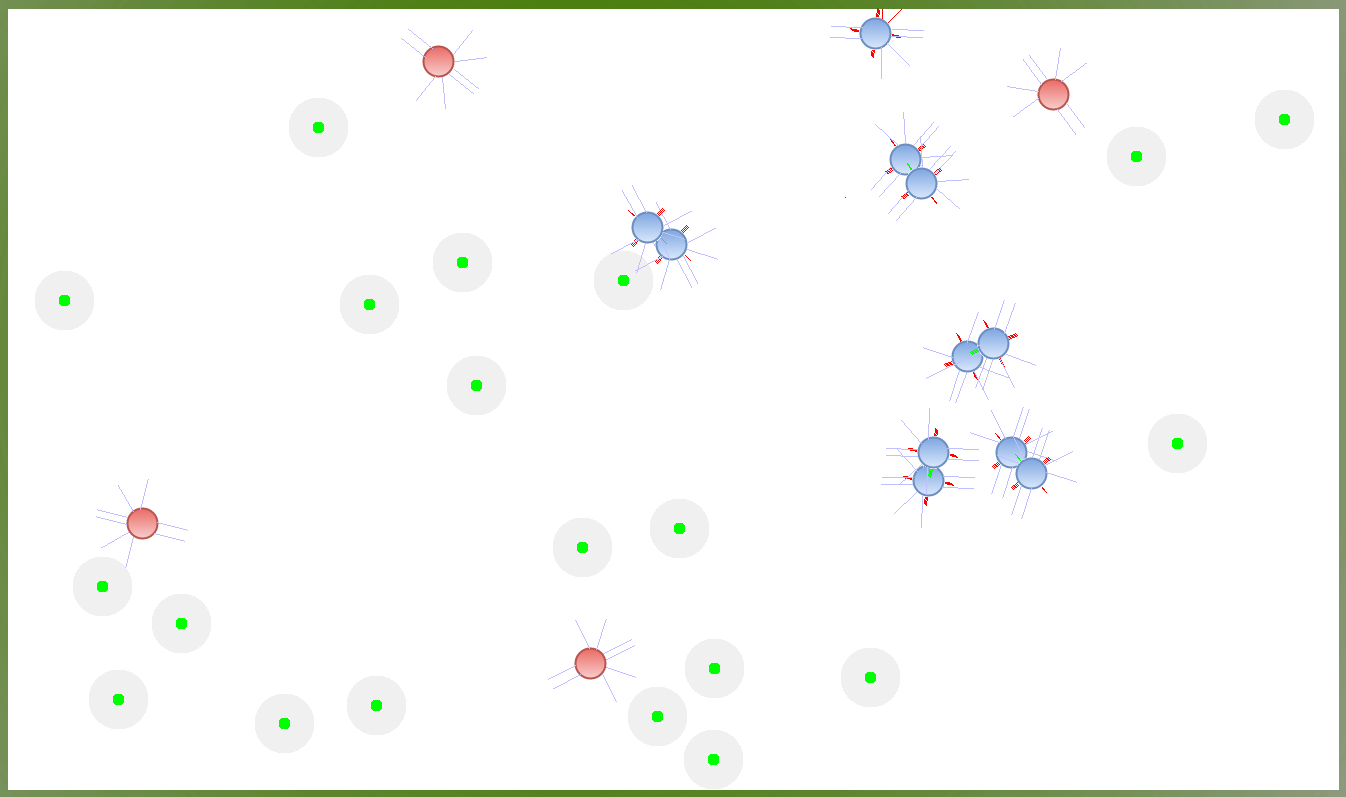
\includegraphics[width=0.65\textwidth]{chapters/res/wall-hug.png}}
	\caption{A robot using its sensors to follow a wall.}
	\label{fig:individual-wall-drive}
\end{figure}


The robot will keep on driving along the wall until it meets another robot, and is able to form a group, or if the sensors detect a robot group passing by.
If a robot group comes within sensor range wile the robot is driving along the wall, the robot will abandon the wall and attempt to follow the group instead.

\subsubsection{Group behaviour}


\begin{figure}[H]
	
	\centering
	\fbox{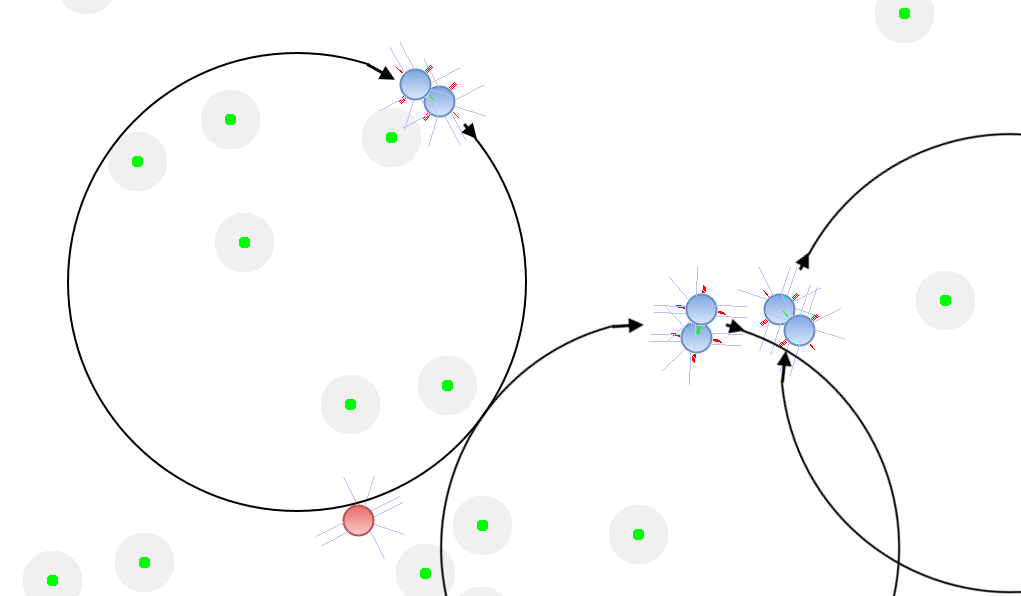
\includegraphics[width=0.65\textwidth]{chapters/res/group_circles.png}}
	\caption{Robot groups driving in circles.}
	\label{fig:group-circles}
\end{figure}

The behaviour of the robot groups is similar to the first mode of the individual robots.
Robot groups also drive in wide circles, displayed in figure \ref{fig:group-circles}, but if the group crashes into a wall it will simply turn around and continue.
The robot groups consume predators in their path, but they make no attempt to follow detected predators.
The robot groups will continue to drive in circles, consuming energy, predators, and making the connections, until the end of the simulation, or until the members of the groups starve.



\section{Discussion}

\subsection{Environmental difficulty analysis}
The robots have two threats in the environments presented, starvation and getting killed by predators.
The robots in the easy environment receive more energy from food, and there is more food available.
From figure \ref{fig:easy-robots-starved} and figure \ref{fig:hard-robots-starved} one can see that this reduces the amount of robots dying from starvation in the easy environment, but the improvement is minuscule.

Increasing the number of predators in the environment seems to have a higher impact on the difficulty presented by an environment.
Figure \ref{fig:easy-robots-eaten} and figure \ref{fig:hard-robots-eaten} shows that increasing the amount of predators present in the environment has a greater impact on the difficulty of the environment than limiting the energy available.
The reason for why increasing the amount of predators has a much higher impact on difficulty is not completely clear from the results.
However, the observed behaviour described in section \ref{sec:invdividual_behaviour} can help explain the results.
The sensors are used by the robot to detect walls and other robots, but not predators or food.
This means that the robot may miss some food, but there is enough food in the environment so the robot will eventually find more food.
On the other hand, failing at predator avoidance has much more severe consequences as the predator will kill the robot.

One of the motivations for this experiment was to see how modifying the evolutionary pressure affects the promotion of self-assembly.
The figures \ref{fig:number-of-groups-easy} and \ref{fig:number-of-groups-hard} shows that the robots form more groups in the easy environment.
At first glance this seems to indicate that the easy environment is more successful at promoting self-assembly.
This difference in number of groups may be explained by examining the lifetime of the robots.
As explained in section \ref{sec:evaluation}, the fitness of a genome is determined by the average lifetime of a robot.
The fitness achieved in the easy environment, figure \ref{fig:easy-fitness}, is higher than than the fitness achieved in the hard environment, figure \ref{fig:hard-fitness}.
This means that the robots in the easy environment live longer, and as a consequence have more time to form groups.

However, figure \ref{fig:group-sizes-easy} and figure \ref{fig:group-sizes-hard} shows that the size of the robot groups formed are not affected by modifying the difficulty of the environment.
In both environments the distribution of group sizes are heavily weighted towards groups of two.
The reason for this may be that the environments gives a high reward for being in a group.
That is protection from predators, but there is no additional reward for forming larger groups.


%One can examine the energy gathering behaviour of the robots 

%39.5, 109.77, 149.27 = 73.54
%24, 65.86, 89.86 = 73.29


\subsection{Port configuration Analysis}
In terms of the results fetched from the port configuration simulations the first obvious remarks stem from the simulation running a three port configuration.
The results in this simulation is much weaker in terms of performance and in terms of promoting self-assembly than the simulations running 2 and 4 connection ports.
The reason for this can not be deduced completely from the empirical results, but as the only difference in these simulations are the number of ports and the alignment it is clear that the connection port configuration can greatly impact the performance of the simulation.
It can also be deduced that it is not the number of connection ports that has the primary impact of the solution, but rather the placement.
The reason one can make this claim is because the configuration using 2 connection ports and 4 connection ports perform quite similar in terms of performance.
If the number of connection ports had a great impact on the results, one would expect the simulation using 2 connection ports or 4 connection ports to yield even poorer results than the 3 connection port simulation.
This narrows the port configuration problem down to the alignment of the connection ports.

\begin{figure}[H]
	\centering
	\begin{subfigure}[b]{0.31\textwidth}
		\centering
		\fbox{\includegraphics[height=\linewidth]{chapters/res/2-ports-robot.png}}
		\caption{2-ports}
	\end{subfigure}
	\begin{subfigure}[b]{0.31\textwidth}
		\centering
		\fbox{\includegraphics[height=\linewidth]{chapters/res/3-ports-robot.png}}
		\caption{3-ports}
	\end{subfigure}
	\begin{subfigure}[b]{0.31\textwidth}
		\centering
		\fbox{\includegraphics[height=\linewidth]{chapters/res/4-ports-robot.png}}
		\caption{4-ports}
	\end{subfigure}
	\caption{The three different port configurations used in simulation}
	\label{fig:robot-port-configuration}
\end{figure}

Figure \ref{fig:robot-port-configuration} shows a closer view of the alignment that the robots initially have when spawned into the environment.
As explained in \ref{moving-ports}, the robots can rotate their connection ports as a group.
A standard strategy which is usually evolved is to either constantly rotate the connection ports in hopes of lining up the ports to another robot, or, the robots start rotating their ports when the sensors see another robot in an effort to self-assemble.
There are two main problems that the 3 connection port robots have compared to the other port configurations.
First, the initial port location does not align to any other robot.


\begin{figure}[H]
	\begin{subfigure}[t]{0.49\textwidth}
		\centering
		\fbox{\includegraphics[height=0.9\linewidth]{chapters/res/3-ports-alignment.png}}
		\caption{Initial alignment}
		\label{3-port-guided-allignment}
	\end{subfigure}
	\begin{subfigure}[t]{0.49\textwidth}
		\centering
		\fbox{\includegraphics[height=0.9\linewidth]{chapters/res/3-ports-alignment-offset.png}}
		\caption{After $50^{\circ}$ port rotation.}
		\label{3-port-guided-allignment-offset}
	\end{subfigure}
	\caption{This figure shows how the 3 connection port robots align}
\end{figure}



As seen in figure \ref{3-port-guided-allignment}, there is not a trivial alignment for the robots to connect.
One might initially presume that this is not a problem as the robots have a mechanism for rotating their ports to solve this exact issue.
However, as all the robots are running the same genome, as per off-line evolution and hence the same behaviour, it becomes increasingly difficult for the robots to solve this problem.
As explained earlier, the robots in this simulation tend to evolve a strategy which involves constantly spinning the connection ports in one direction.
But, as seen in figure \ref{3-port-guided-allignment-offset}, in the case where all robots at some time step have rotated their connection ports $50^{\circ}$, the same issue of port alignment would still hold.

\begin{figure}[H]
	\begin{subfigure}[t]{0.49\textwidth}
		\centering
		\fbox{\includegraphics[height=0.9\linewidth]{chapters/res/2-ports-alignment.png}}
		\caption{This figure shows how the 3 connection port initially align.}
		\label{2-port-guided-allignment}
	\end{subfigure}
	\begin{subfigure}[t]{0.49\textwidth}
		\centering
		\fbox{\includegraphics[height=0.9\linewidth]{chapters/res/4-ports-alignment.png}}
		\caption{This figure shows how the 3 connection ports align after all robots rotate their connection ports $50^{\circ}$.}
		\label{4-port-guided-allignment}
	\end{subfigure}
	\caption{This figure shows how the 2 and 4 connection ports robots align}
	\label{2-4-port-guided-allignment}
\end{figure}

Consider figure \ref{2-4-port-guided-allignment}.
In this example there are two and four port configurations.
It can be observed that with initial rotation of the ports, there exists possibilities for the robots to self-assemble without having the robots behave differently in terms of rotating their connection ports.
This differentiation seems to be the main reason that the 3 connection port configuration is being outperformed.

The second problem robots with 3 connection ports, in this alignment, is the possible architecture the robots can form.
Chapter \ref{ch:background} covers the chain and lattice architectures that the robots can form when self-assembling. %needs ref/explain
The simulator is developed to support the lattice architecture because if its simplistic method of coordinated movement.





























\clearpage

\chapter{Conclusion}
\label{ch:conclusion}
The main focus and goal of this thesis have been to discover and test the elements present in a self-assembly system when robots are given basic learning capabilities.
The experiment has been conducted using a heavily modified version of the roborobo framework.
The main factors that have been researched in accordance with self-assembly have been: connection port configuration, environmental influence and local communication.

The results obtained from the connection port simulations, show that configuration of the connection ports can significantly impact the emergence of self-assembly using an evolutionary algorithm.
The port configuration consists of the number of connection ports each robot has available and the relative positioning of the connection ports on the robot.
Both elements influence the size and frequency of self-assembling robot groups.
It can, however, be narrowed down to a single influential self-assembly mechanism: the assembly protocol.
It is evident from the results that providing the robots with tools that allow an efficient and simple assembly protocol to be evolved, is essential to achieve successful results.

The main focus of the learning algorithm should be to solve the task at hand and not deriving a complex strategy for achieving self-assembly.
Having the ability to form a complex assembly protocol can be appropriate in a particular situation as it may significantly improve performance.
However, it should not be a minimum requirement for the ability to self-assemble.
An evolutionary algorithm performs better when an incremental solution to some desired behaviour is possible.
If the least complex achievable self-assembly protocol requires sufficiently advanced cognition, then the robots may only have a few occurrences of self-assembly or none at all.

The results gained from the environment difficulty simulations implies that the difficulty of the environment is not directly correlated with promoting self-assembly.
The results show that the robots perform better in an easy environment, but this is rather due to restrictions in the environment and not due to the ability to self-assemble.
The only effect that difficult environments impose on self-assembly is making robots die earlier, giving them fewer opportunities to self-assemble.
Promoting self-assembly may rather see a larger impact if the rules of the environment change(examples include translation speed of predators and the physical size of the environment).

One of the problem statements this study aimed to examine was the introduction of a local communication module. From the results discussed in chapter  \ref{ch:results_and_discussion}, it was seen that using the local communication module drastically changed the behaviour of self-assembled groups. 
From this experiment, it cannot be made any conclusive remarks as to the local communication module promoting the robots to self-assemble as deciphering the evolved values of the neural network is very difficult.
From a logical point of view, one would not expect there to be a difference, because the local communication module only transmits information between the robots in a self-assembled group. 
Hence, there is seemingly no reason why this would help two singular robots to self-assemble.
However, when using an evolutionary algorithm, the use of certain modules may be utilised differently than the developer predicts.
The evolved genomes may use the module as a state machine instead of a message passing module.

In concluding remarks, it is shown that there should be a larger focus on the connection mechanism which the robots have equipped.
To promote self-assembly, the ideal hardware mechanisms would be one which makes it easy for the robots to evolve an efficient assembly protocol, but also yields an interface to evolve complex assembly behaviour.
In the case where static connection points are used, using many, initially aligned connection ports increase the frequency and size of the self-assembled groups.
The difficulty of the environment does not seem to impact the frequency of self-assembly, and one may consider altering the static rules of the environment which may yield a noticeable impact.
A local communication module is an advantageous asset to provide for self-assembly robots as it may be used to communicate a transition to group behaviour as well as assisting in the type of behaviour which emerges from the group. 
  


\section{Future work}
From the observed results of self-assembly mechanisms and environment, it is seen that improvements and further experimentation can be implemented. 
This forms the basis for exploring other factors of self-assembly mechanisms.

The port configuration has the possibility to be explored further as the results of this study determined that it has a significant impact on the emergence of self-assembly. 
A possible exploratory field would be to challenge the static nature of the ports presented in this study.
Hardware mechanisms which do not depend on fixed positions on a robot where the robots are able to self-assemble at any point on a connecting robot should, according to the results obtained in this study, perform at a higher rate.
An obvious end goal of studies like this one is to be able to realise these robots into the real world.
In these scenarios, the reality gap will probably inflict even stricter conditions on performing a simple assembly strategy which could detriment the ability to self-assemble.

Since the impact of changing the environment did not suggest a change in assembly protocol or strategy, a reasonable continuation would be to categorize which environmental scenarios self-assembly, through evolution, is most appropriate. 
Changing the atomic rules of the environment and robot problem tasks may yield results indicating scenarios where evolutionary self-assembly is more appropriate.

Local communication is a mechanism which has not been significantly researched in this field. 
According to the results obtained in this study, further exploration into communication modules between the robots can give rise to increasingly complex behaviour.
In this study, a very simple protocol of passing floating point numbers from one robot to another was implemented.
Perhaps there are better communication protocols available which could further the performance.
It is also possible to look at the possibility for robots to communicate on a local spectrum where they are not necessarily self-assembled.
Expanded local communication may improve their ability to form an effective assembly strategy through evolution.

The evolutionary algorithm used in this study is simple and standard.
There exists additionally advanced evolutionary algorithms and other bio-inspired algorithms where the mechanisms presented in this study should be additionally explored.
\clearpage

\nocite{*}

\bibliographystyle{abbrv}

\bibliography{references} 

\end{document}